%The following line prevents the headers and the \begin{document}\end{document}
%from being executed in the individual files.
\def\whole{}
\documentclass[leqno]{book}
%\usepackage{msri
\input style-for-curves.sty
\usepackage{hyperref}
\usepackage{msribib}
\usepackage{pdfpages}
\usepackage{draftwatermark}
\SetWatermarkText{DRAFT:\ \ \today}
\SetWatermarkScale{3}
\SetWatermarkColor[gray]{0.9}

%\input header.tex 

%\documentclass{cambridge7A}
%\usepackage{ag2}
\usepackage{xcolor}
%\usepackage{mtpro2}
%\usepackage{times}
%\usepackage{hatcher}
%\usepackage{msribib,local}
%\usepackage{geompsfi}

\errorcontextlines=1000

%\usepackage{makeidx}
\makeindex
% \index{word} in the doc; \index{variety!algebraic} gives variety, algebraic
% PUT a % after each \index{***}

\overfullrule=5pt
\catcode`\@\active
\def@{\mskip1.5mu} %produce a small space in math with an @

%%the following allows flexible naming of chapters, but then the sections don't appear in the toc
\newcommand{\mychapter}[2]{
    \setcounter{chapter}{#1}
    \setcounter{section}{0}
    \chapter*{#2}
    \addcontentsline{toc}{chapter}{#2}
}

\title{Practical Curves}
\author{\copyright David Eisenbud and Joe Harris}
%\includeonly{2-RR, 5-Curvesofgenus2and3}
%\includeonly{5-Curvesofgenus2and3}
%\includeonly{0-intro, 1-LinearSeries, 2-RR, 3-CurvesOfGenus0And1, 4-Jacobians, 5-Curvesofgenus2and3}
%\includeonly{0-intro, 1-LinearSeries, 2-RR, 3-CurvesOfGenus0And1, 4-Jacobians, 5-Curvesofgenus2and3}
%\includeonly{0-intro, 1-LinearSeries, 2-RR, 3-CurvesOfGenus0And1, 4-Jacobians, 5-Curvesofgenus2and3, 7-Curvesofgenus45}
%\includeonly{2-RR}
%\includeonly{1-LinearSeries, 2-RR, 3-CurvesOfGenus0And1, 4-Jacobians}
%\includeonly{12-HilbertSchemes, 13-HilbertSchemesII }
%\def\all{toc,out1,chern,out2,lefschetz,out3,bib,ind, out1a}
%\includeonly{\all}

\begin{document}
\maketitle

\pagenumbering{roman}
\setcounter{page}5
\pagenumbering{arabic}
\tableofcontents

%\mychapter{1}{1 Linear Systems}
%header and footer for separate chapter files

\ifx\whole\undefined
\documentclass[12pt, leqno]{book}
\usepackage{graphicx}
\input style-for-curves.sty
\usepackage{hyperref}
\usepackage{showkeys} %This shows the labels.
%\usepackage{SLAG,msribib,local}
%\usepackage{amsmath,amscd,amsthm,amssymb,amsxtra,latexsym,epsfig,epic,graphics}
%\usepackage[matrix,arrow,curve]{xy}
%\usepackage{graphicx}
%\usepackage{diagrams}
%
%%\usepackage{amsrefs}
%%%%%%%%%%%%%%%%%%%%%%%%%%%%%%%%%%%%%%%%%%
%%\textwidth16cm
%%\textheight20cm
%%\topmargin-2cm
%\oddsidemargin.8cm
%\evensidemargin1cm
%
%%%%%%Definitions
%\input preamble.tex
%\input style-for-curves.sty
%\def\TU{{\bf U}}
%\def\AA{{\mathbb A}}
%\def\BB{{\mathbb B}}
%\def\CC{{\mathbb C}}
%\def\QQ{{\mathbb Q}}
%\def\RR{{\mathbb R}}
%\def\facet{{\bf facet}}
%\def\image{{\rm image}}
%\def\cE{{\cal E}}
%\def\cF{{\cal F}}
%\def\cG{{\cal G}}
%\def\cH{{\cal H}}
%\def\cHom{{{\cal H}om}}
%\def\h{{\rm h}}
% \def\bs{{Boij-S\"oderberg{} }}
%
%\makeatletter
%\def\Ddots{\mathinner{\mkern1mu\raise\p@
%\vbox{\kern7\p@\hbox{.}}\mkern2mu
%\raise4\p@\hbox{.}\mkern2mu\raise7\p@\hbox{.}\mkern1mu}}
%\makeatother

%%
%\pagestyle{myheadings}

%\input style-for-curves.tex
%\documentclass{cambridge7A}
%\usepackage{hatcher_revised} 
%\usepackage{3264}
   
\errorcontextlines=1000
%\usepackage{makeidx}
\let\see\relax
\usepackage{makeidx}
\makeindex
% \index{word} in the doc; \index{variety!algebraic} gives variety, algebraic
% PUT a % after each \index{***}

\overfullrule=5pt
\catcode`\@\active
\def@{\mskip1.5mu} %produce a small space in math with an @

\title{Personalities of Curves}
\author{\copyright David Eisenbud and Joe Harris}
%%\includeonly{%
%0-intro,01-ChowRingDogma,02-FirstExamples,03-Grassmannians,04-GeneralGrassmannians
%,05-VectorBundlesAndChernClasses,06-LinesOnHypersurfaces,07-SingularElementsOfLinearSeries,
%08-ParameterSpaces,
%bib
%}

\date{\today}
%%\date{}
%\title{Curves}
%%{\normalsize ***Preliminary Version***}} 
%\author{David Eisenbud and Joe Harris }
%
%\begin{document}

\begin{document}
\maketitle

\pagenumbering{roman}
\setcounter{page}{5}
%\begin{5}
%\end{5}
\pagenumbering{arabic}
\tableofcontents
\fi


\setlength{\parskip}{5pt}

\addtocounter{chapter}{-1}
\chapter{Introduction}
\label{IntroChapter}

\section{Why you want to read this book}

Algebraic geometry is an old subject. Descartes' introduction in 1637 of coordinates in the plane and in space made it possible to relate the algebra of polynomials to the geometry of their zero loci. Gauss' proof of the Fundamental Theorem of Algebra showed that the degree of a polynomial, an algebraic invariant, was equal to the number of roots counted with multiplicity, a geometric invariant. Mathematicians have been doing what is recognizably algebraic geometry for more than two centuries.

Within algebraic geometry, the study of algebraic curves is the oldest topic. Newton already classified all the possible types of real affine cubics. By the middle of
the 19th century a rich theory of curves in the complex projective plane was a central topic, overturned by Riemann's work in mid-century---what became the theory of Riemann surfaces, which introduced new techniques of complex analysis into the field. This was  taken up and made algebraic as a theory of plane curves by Alexander Brill, Max Noether, F. S. Macaulay and many others. By the end of the century Halphen and others were interested in the classification of space curves as well. The interested reader will find more about the
early work on algebraic curves in the Appendix to this book, written by historian Jeremy Gray.

The development continues unabated today: in the second half of the 20th century Grothendieck's foundations led to the solution of many classical problems and, in particular, to a firm foundation for the theory of moduli, allowing mathematicians to exploit the fact that algebraic varieties generally come in families parameterized by other algebraic varieties---something that we will return to often in this book. Algebraic geometry has merged more and more with number theory, and the moduli space of curves plays an important role in string theory, responding to the needs of physicists.

For these reasons, the subject of algebraic curves is one of the richest in algebraic geometry, if not in all of mathematics. If you want to know whether a conjecture is plausible, you can generally find well-understood special cases on which to test it. Some of the fundamental constructions of algebraic geometry, like the construction of moduli spaces and their description, can be carried out in the setting of algebraic curves with a degree of precision and detail far beyond what has been possible in higher dimensions. 

Already the geometry of plane curves of degrees 3 and 4 shows some of the promise of the subject:

Every smooth plane cubic has exactly 9 flexes---points where the tangent line has contact of order 3 with the curves---and these points form a remarkable configuration; they're the only known example of a finite, non-colinear set of points in the plane such that the line joining any two contains a third. Generalizing the notion of the flexes of a plane cubic leads us to the subject of inflectionary behavior of linear series on curves in general, which arose separately in the theory of Weierstrass points on Riemann surfaces, and  has become a powerful tool. 

\pict{small pictures illustrating this could go here}

Every smooth quartic curve has exactly 28 bitangents, also forming a beautiful and mysterious configuration; see
Figure~\ref{28bitangents}. In \cite{MR0115124}, first published in 1837, Salmon computed the number (315) of 4-tuples of bitangents whose eight points of tangency lie on a conic. The extension of these ideas to curves of higher genus leads us to the rich theory of theta-characteristics, bringing together algebra (in the form of a bilinear pairing on the points of order 2 in the Jacobian of a curve), analysis (in the form of theta-functions) and of course projective geometry.

The richest subject in what is arguably the richest branch of mathematics\footnote{Number theorists may quibble}---of course you want to read this book! 

\section{Why we wrote this book}

The wealth of beauty, both in theory and in examples, certainly makes the study of algebraic curves an attractive prospect. But it comes at a price: to absorb in detail all the things we've learned over the centuries about algebraic curves would take years, if not decades. This is, in essence, the conundrum facing anyone who undertakes to write a book on the subject: how to convey the wealth of information  (and the many many ways in which our knowledge is incomplete) without writing an encyclopedia. We have chosen to try to be useful and broad but not necessarily complete. 

When we introduce a technique or a construction without full proofs, we do so as a ``cheerful fact'', in a different font, 
and we try to make clear which category is which.\footnote{Hats off to the Berkeley ``Many cheerful facts'' seminar run
by the graduate students, which gave us this idea!}''

\begin{quote}\it{I'm very well acquainted, too, with matters mathematical,\\
I understand equations, both the simple and quadratical,\\
About binomial theorem I am teeming with a lot o' news,\\
With many cheerful facts about the square of the hypotenuse.}
\end{quote}
---Gilbert and Sullivan, Pirates of Penzance, Major General's Song


Our intended audience is a graduate student considering working in the field of algebraic curves, or a researcher in a related field whose work has led them to questions about algebraic curves. Our goal is to equip the reader with the understanding of both the techniques and the state of our knowledge necessary to read the current literature and work on open problems.

\section{What's Practical?}

\begin{quote}
Be simple by being concrete. Listeners are prepared to
accept unstated (but hinted) generalizations much more than they are able, on the spur of the moment, to
decode a precisely stated abstraction and to re-invent the special cases that motivated it in the first place. 
\end{quote}

--Paul Halmos, How to Talk Mathematics

Although mathematicians aspire to understand their subjects deeply, we feel that we learn in stages: in early stages we accept large and difficult results as black boxes and explore the rich examples that they yield. That is how we have tried to organize this book: 
We begin with two chapters that we hope will bridge the gap between first courses in algebraic geometry/commutative algebra at the level of Fulton's or  Reid's well-known books \cite{Fulton1989}, \cite{MR982494} and the professional language of invertible sheaves, cohomology and linear series. An ideal background would
be Hartshorne's book \cite{Hartshorne1977} or Vakil's notes \cite{Vakil-notes} but in \emph{practice} very much less will suffice if the reader is willing to accept some advanced ideas or look them up at leisure---we have tried to give precise references where this might be required. Subsequent chapters roughly alternate between expositions of basic techniques (partly without proofs) and families of examples, treated in detail. 

We love T. S. Eliot's book, \emph{Old Possum's Book of Practical Cats}, a collection of light verse introducing a collection of cats with distinct personalities. In a way, our approach in the chapters of examples reflects Eliot's: different areas and questions under the general umbrella of algebraic curve theory have distinct aspects---personalities, if you will.


\section{What's in this book}
In organizing this book we faced a common problem of  mathematical exposition:
\begin{quote}
\small\sf
We are dealing here with a fundamental and almost paradoxical difficulty. Stated briefly, it is that learning is sequential but knowledge is not. A branch of mathematics... consists of an intricate network network of interrelated facts, each of which contributes to the understanding of those around it. When confronted with this network for the first time, we are forced to follow a particular path, which involves a somewhat arbitrary ordering of the facts.

--Robert Osserman\cite{Poetry}

\end{quote}

In Chapters~\ref{linear series} and~\ref{RiemannRochChapter} we lay out the central objects of algebraic curve theory: invertible sheaves, linear systems, canonical sheaves and the Riemann-Roch theorem, as well as
Hurwitz' theorem,
the adjunction formula and  some elementary facts about the geometry of surfaces. We prove or sketch the
proofs of many of these basic results. These chapters may serve as review for someone who has been exposed already to material roughly equivalent to Chapter IV of \cite{Hartshorne1977}. 

Thereafter, we alternate between chapters focussed on special cases and chapters developing more of the theory. Chapter~\ref{genus 0 and 1 chapter}  describes the geometry of curves of genus 0 and 1 in projective space. We emphasize some of the things that make rational normal curves so special, and take the opportunity to introduce the conditions implying that a curve is \emph{arithmetically Cohen-Macaulay}. We describe the low-degree linear series on curves of genus 1, and demonstrate how counts of parameters suggest the presence of a moduli space. 

In genus $\geq 2$ there is a fundamental shift: not all invertible sheaves of a given degree on a curve $C$ of genus $g \geq 2$ are congruent modulo the automorphism group of the curve.
It is a salient feature of algebraic geometry that families of similar algebro-geometric objects are often naturally parameterized by algebraic varieties. This idea goes back to the beginning of algebraic geometry and the family of plane curves of degree $d$, but was only fully clarified in the work of Grothendieck, Deligne and Mumford,

Chapter~\ref{Jacobians chapter} introduces our first examples of this phenomenon: the \emph{fine moduli spaces} of divisors on a curve, as well as the Jacobian, for which we give the classic analytic construction, and the Picard varieties $\Pic_d(C)$ parametrizing isomorphism classes of invertible sheaves. We also introduce the subvarieties $W^{r}_{d}(C)$ parametrizing invertible sheaves with many sections. 

 Since the Jacobian is irreducible, we can speak meaningfully of a \emph{general} invertible sheaf, and of the dimension of various families of special invertible sheaves. With this in hand we prove
that every curve of genus $g>1$ can be embedded in $\PP^{3}$ as a curve of degree $g+3$.

Equipped with information about the Jacobian, we proceed in Chapter~\ref{genus 2 and 3 chapter} to study curves of genus 2 and 3, describing in particular how the geometry of maps of our curve to projective space given by sections of invertible sheaves depends on the sheaf. We show how a hyperelliptic curve of genus $g$
can be described by a set of $2g+2$ points in $\PP^{1}$, and we describe the canonical maps. Again, this
suggests the existence of moduli spaces.

We spend Chapters~\ref{ModuliChapter} and~\ref{CurvesModuli chapter} on other moduli spaces as they appear in the world of curves, though we do not give complete proofs of all the assertions made. We start in Chapter~\ref{ModuliChapter} with some central examples of fine moduli spaces, primarily
the Hilbert scheme. Using properties of the Hilbert scheme we show that curves of genus $\geq 2$
can have only finitely many automorphisms, and more generally that there can only be finitely
many morphisms from one such curve to another.

The most interesting example of a moduli space, the moduli of smooth (or stable) curves of genus $g$, is not a fine moduli space, and we spend Chapter~\ref{CurvesModuliChapter} describing what it is and isn't. In that chapter we also describe the Hurwitz space of coverings and the Severi variety of nodal plane curves.

After this, it's back to examples: in Chapter~\ref{genus 4, 5 Chapter} we analyze aspects of the geometry of curves of genus 4 and 5.  

In the following two chapters we take up 
the properties of the points of a general hyperplane sections of a curve in projective space. 
In Chapter~\ref{linear general position chapter} we give Rathmann's proof that
the points of a general hyperplane section of a reduced irreducible curve are in linearly general position (independent of the characteristic).
Consequences include Castelnuovo's bound  on the maximal genus of curves of a given degree.
We show that the curves that achieve the maximum genus, called Castelnuovo curves,
are arithmetically Cohen-Macaulay. These include all plane curves, as well as
canonical curves and linearly normal curves of high degree compared to their genera. 

We also
use the linear general position result to prove the strong forms of Clifford's and Martens' theorems
on special linear series; to show that every curve has a nodal plane model; and to show that a 
general invertible sheaf  of degree $g+2$ on a curve of genus $g$  maps the curve to a nodal curve
in the plane---unless the curve is hyperelliptic, in which case the image has a single multiple point of
multiplicity $g$.

In characteristic 0 an even stronger statement than linearly general position is true: the monodromy of the hyperplane divisors is the full symmetric group. We take up this
and some other monodromy questions in Chapter~\ref{uniform position} and prove consequences
for secant planes and for sums of linear series.

In Chapter~\ref{Brill-Noether} we return to the general question: ``What linear series exist on curves of genus $g$?" We give three possible interpretations of this question, and the answers to each: Clifford's theorem, the Castelnuovo bound, and the Brill-Noether theorem, postponing the proof of the latter. 
We apply the Brill-Noether result to explore  various special classes of curves of genus 6.

Chapter~\ref{inflections chapter} prepares for the proof of the Brill-Noether theorem 
with a discussion of inflection points of linear series, generalizing the flexes of plane curves. The Pl\"ucker formula
counts the number of inflection points, with appropriate weights. In this chapter we explain
the remarkable connection between the study of inflections on a rational curve and the Schubert calculus of cycles in the Grassmannian. In Chapter~\ref{BrillNoetherproofChapter} we use this material, together with a degeneration to cuspidal rational curves, to give a relatively short proof of the Brill-Noether theorem.

In Chapter~\ref{PlaneCurvesChapter} we take the classical point of view of Brill and Noether,
and describe an explicit algorithm for finding the complete linear series on a smooth curve, using a singular plane model. This involves the result classically known as the completeness of the adjoint linear series. For the general case we use a simple case of the theory of dualizing sheaves, introduced in more generality in the next chapter.

Returning to curves in $\PP^{3}$ in Chapter~\ref{LinkageChapter} we explain the theory of Hartshorne and Rao classifying curves up to linkage. This theory applies to all purely 1-dimensional subschemes of $\PP^{3}$, and to explain this
we detour to discuss dualizing sheaves and Grothendieck's $f^{!}$ operation.

Curves that lie on a quadric in $\PP^3$ are easy to understand. In Chapter~\ref{ScrollsChapter} we systematically describe a natural generalization: rational normal scrolls and the curves that lie on them. This includes all the Castelnuovo curves of high degree. 

Chapter~\ref{SyzygiesChapter} presents some aspects of the theory of syzygies of the homogeneous ideals of curves and the the famous---and, as of this writing, open---conjecture of Mark Green that connects syzygies of canonical curves to the Clifford index and the theory of rational normal scrolls. A table reproduced from work of Frank-Olaf Schreyer shows the sensitivity of the numerical information in the free resolution of a canonical curve to questions of the existence of special linear series on the curve.

Chapter~\ref{HilbertSchemesChapter} is in some ways the culmination of the book. It is concerned with \emph{Hilbert schemes}, schemes $\cH_{g,3,d}$ that parametrize smooth curves of genus $g$ and degree $d$  in $\PP^3$. We work out examples up to degree 7, define the ``principal component"---the only one dominating the moduli space of curves---and derive dimension estimates from deformation theory and from the Brill-Noether theorems
using most of the ideas we have introduced. 

The historical appendix written by Jeremy Gray, Chapter~\ref{Appendix-History},  is a survey of some of the work on
algebraic curves up to that of Brill and Noether, and we are grateful to him for allowing us to include it.

\subsection{Relation of this book to other texts} 
Chapter IV of~\cite{Hartshorne1977} has a similar flavor to that of this book, and contains details of most of the 
results in our Chapters~\ref{linear series} and~\ref{RiemannRochChapter}. A beautiful (and brief) account of a number of topics in a style we particularly admire is found in \cite{MumfordCJ}.

A far more extensive treatment, partially overlapping that of the present book and containing many other topics, can be found in the important and encyclopaedic~\cite{ACGH} and~\cite{ACG}, and yet even these works do not cover all the major topics in the field. 
One of the topics we do not cover is the construction of the moduli space of curves, which can be found
in~\cite{ACG}. Though not a complete account,~\cite{HarrisMorrison1998} deals directly with this
topic. 

There are more elementary accounts of some of our material, in~\cite{Fulton1989} and \cite{Walker1978} (who goes farther than we do into local resolution of singularities) as well as~\cite{Griffiths-curves}. The book~\cite{Kunz} treats plane curves and their normalizations via the theory of valuations, and contains a detailed  account of the ideas we treat in Chapter~\ref{PlaneCurvesChapter} from this more algebraic point of view.  A comprehensive treatment of the local topological theory of plane curves and their singularities in \cite{Brieskorn1986}. The topological questions there are developed in different directions in~\cite{MR0239612} %Milnor
 and~\cite{MR817982}. %Eisenbud-Neumann}. 
 An  idiosyncratic collection of interesting topics is presented in~\cite{Clemens-Scrapbook}.

 The Riemann surface point of view is well represented in the books \cite{Forster}, \cite{Gunning}, \cite{Gunning-2}, \cite{Kirwan}, and \cite{Miranda}. 


\section{Prerequisites, notation and conventions}
The reader should be familiar with the (Krull) dimension of rings and varieties, and their primary decomposition at the level of \cite{Atiyah-MacDonald}. Ideally the reader  will already have some familiarity with the geometry of curves and surfaces
at the level of \cite[Chapter IV]{Hartshorne1977} and the beginning of Chapter V, there, though our summary of the necessary material in the first two chapters of this book may suffice for the intrepid.

Unless otherwise mentioned, we assume that the ground field is the field of complex numbers $\CC$, though much of what we do
could be done over any field.

\subsection{Commutative Algebra} 
All the rings we consider are commutative with unit and Noetherian.

Since we are working over  a field of characteristic 0, we use the terms smooth and nonsingular interchangeably when
referring to a point on a scheme.

Some results that we use:
 \begin{theorem}[Lasker's Theorem]\label{Lasker}
If $f_1,\dots, f_c \subset \CC[x_0,\dots, x_n]$ generates an ideal of codimension $c$, then 
the ideal $(f_1,\dots, f_c)$ is unmixed (all its primary components have codimension $c$).
\end{theorem}

\begin{theorem}\label{finiteness of normalization}
 If $R$ is a domain that is a finitely generated algebra over a field or a localization of such an algebra, then the
normalization ($=$ integral closure) of $R$ is a finitely generated $R$-module.
If $R$ is 1-dimensional, then its normalization is nonsingular.
\end{theorem}

\subsection{Projective geometry}
 
Schemes are assumed quasi-projective, and \emph{varieties} (including curves) are reduced and irreducible schemes unless otherwise stated. ``Points'' will always be closed points unless we explicitly say otherwise. 
{\bf Note to the patient reader: We usually use the term curve to refer to a smooth irreducible projective purely 1-dimensional scheme, but the usage in this DRAFT is not completely consistent.}

Though we occasionally use the classical topology, 
the term ``open set'' refers to the Zariski topology unless otherwise stated.

The results we assume are
 well-represented by the following classical theorems:

\begin{theorem}[B\'ezout's Theorem]
If $X,Y\subset \PP^r$ are subvarieties, and if $\codim(X\cap Y) = \codim X + \codim Y$,
then $\deg (X\cap Y) = \deg(X)\deg(Y)$.
\end{theorem}

\begin{theorem}[Bertini's Theorem]\label{Bertini}
If $X\subset \PP^r$  is a nonsingular quasi-projective variety, and $\{H_\lambda \mid \lambda\in \Lambda\}$ is a linear family of hyperplanes of $\PP^r$, then for an open subset of $\lambda\in \Lambda$ the scheme $H_\lambda \cap X$ is nonsingular away from the union of the \emph{base locus}
$
\cap_{\lambda \in \Lambda} H_\lambda
$
and the singular locus of $X$.
\end{theorem}

\begin{theorem}[Main theorem of elimination theory]
 Any morphism $\phi: X\to Y$ of projective varieties (or schemes) is closed: if $X'\subset X$ is a Zariski closed subset,
 then $\phi(X') \subset Y$ is also closed.
\end{theorem}

\begin{corollary}
If $\phi: C\to D$ is a non-constant morphism of (projective) curves, then $\phi$ is finite and surjective. 
\end{corollary}

If $D$ is a 
smooth curve then the local ring of $D$ at any point is a discrete valuation ring, so any torsion free module is flat. 
Thus:

\begin{proposition}
If $\phi: C\to D$ is a non-constant morphism of smooth curves, then $\phi$ is finite, surjective, and flat.
\end{proposition}

If $X\subset \PP^{r}$ is any scheme, we define the \emph{homogeneous coordinate ring} of $X\subset \PP^{r}$
to be $R_{X} = R_{X/\PP^{r}}:= S/I(X)$, where $S =\CC[x_{0}, \dots, x_{r}]$ is the homogeneous coordinate ring of $\PP^{r}$. We emphasize
that, unlike the coordinate ring of an affine variety, this is not an intrinsic invariant of $X$, but depends on the 
embedding in $\PP^{r}$. 

\subsection {Sheaves and cohomology} 

Some familiarity with coherent sheaves is recommended; a possible source is
the first chapter of our book \cite{GeomSchemes}. 
As for cohomology, it is probably enough if the reader can write down $H^i$ and exact sequences without blushing.
In any case we review some of the theory of coherent sheaves and their cohomology theory, and that of divisors on projective 
varieties, in the first two Chapters. 

We occasionally use the bijection between algebraic and analytic sheaves on smooth projective curves, which preserves
cohomology and exact sequences. This is a special case of the results in \cite{GAGA}. 

If $\sF$ is a sheaf on $X$ and $X\subset Y$ then we will identify $\sF$ with
the sheaf usually written $\iota_*\sF$, where $\iota:X\to Y$ is the inclusion map,
 and thus regard $\sF$ as a sheaf on $Y$ as well.
The cohomology  $H^i(X, \sF) = H^i(Y,\iota_*\sF)$ canonically, so we will
simply and unambiguously write $H^i(\sF)$ for either of these. 

We write $h^i(\sF)$ or (if $D$ is a divisor) $h^{i}(D)$ for 
$\dim_{\CC}H^i(\sF)$ or $\dim_{\CC}H^i(\cO_X(D))$. 

If $\sF$ is a sheaf on projective space (perhaps supported on a subvariety) we write $H^i_*(\sF)$ for
$\oplus_{m\in \ZZ} H^i(\sF(m))$. 



%footer for separate chapter files

\ifx\whole\undefined
%\makeatletter\def\@biblabel#1{#1]}\makeatother
\makeatletter \def\@biblabel#1{\ignorespaces} \makeatother
\bibliographystyle{msribib}
\bibliography{slag}

%%%% EXPLANATIONS:

% f and n
% some authors have all works collected at the end

\begingroup
%\catcode`\^\active
%if ^ is followed by 
% 1:  print f, gobble the following ^ and the next character
% 0:  print n, gobble the following ^
% any other letter: normal subscript
%\makeatletter
%\def^#1{\ifx1#1f\expandafter\@gobbletwo\else
%        \ifx0#1n\expandafter\expandafter\expandafter\@gobble
%        \else\sp{#1}\fi\fi}
%\makeatother
\let\moreadhoc\relax
\def\indexintro{%An author's cited works appear at the end of the
%author's entry; for conventions
%see the List of Citations on page~\pageref{loc}.  
%\smallbreak\noindent
%The letter `f' after a page number indicates a figure, `n' a footnote.
}
\printindex[gen]
\endgroup % end of \catcode
%requires makeindex
\end{document}
\else
\fi



%header and footer for separate chapter files

\ifx\whole\undefined
\documentclass[12pt, leqno]{book}
\usepackage{graphicx}
\input style-for-curves.sty
\usepackage{hyperref}
\usepackage{showkeys} %This shows the labels.
%\usepackage{SLAG,msribib,local}
%\usepackage{amsmath,amscd,amsthm,amssymb,amsxtra,latexsym,epsfig,epic,graphics}
%\usepackage[matrix,arrow,curve]{xy}
%\usepackage{graphicx}
%\usepackage{diagrams}
%
%%\usepackage{amsrefs}
%%%%%%%%%%%%%%%%%%%%%%%%%%%%%%%%%%%%%%%%%%
%%\textwidth16cm
%%\textheight20cm
%%\topmargin-2cm
%\oddsidemargin.8cm
%\evensidemargin1cm
%
%%%%%%Definitions
%\input preamble.tex
%\input style-for-curves.sty
%\def\TU{{\bf U}}
%\def\AA{{\mathbb A}}
%\def\BB{{\mathbb B}}
%\def\CC{{\mathbb C}}
%\def\QQ{{\mathbb Q}}
%\def\RR{{\mathbb R}}
%\def\facet{{\bf facet}}
%\def\image{{\rm image}}
%\def\cE{{\cal E}}
%\def\cF{{\cal F}}
%\def\cG{{\cal G}}
%\def\cH{{\cal H}}
%\def\cHom{{{\cal H}om}}
%\def\h{{\rm h}}
% \def\bs{{Boij-S\"oderberg{} }}
%
%\makeatletter
%\def\Ddots{\mathinner{\mkern1mu\raise\p@
%\vbox{\kern7\p@\hbox{.}}\mkern2mu
%\raise4\p@\hbox{.}\mkern2mu\raise7\p@\hbox{.}\mkern1mu}}
%\makeatother

%%
%\pagestyle{myheadings}

%\input style-for-curves.tex
%\documentclass{cambridge7A}
%\usepackage{hatcher_revised} 
%\usepackage{3264}
   
\errorcontextlines=1000
%\usepackage{makeidx}
\let\see\relax
\usepackage{makeidx}
\makeindex
% \index{word} in the doc; \index{variety!algebraic} gives variety, algebraic
% PUT a % after each \index{***}

\overfullrule=5pt
\catcode`\@\active
\def@{\mskip1.5mu} %produce a small space in math with an @

\title{Personalities of Curves}
\author{\copyright David Eisenbud and Joe Harris}
%%\includeonly{%
%0-intro,01-ChowRingDogma,02-FirstExamples,03-Grassmannians,04-GeneralGrassmannians
%,05-VectorBundlesAndChernClasses,06-LinesOnHypersurfaces,07-SingularElementsOfLinearSeries,
%08-ParameterSpaces,
%bib
%}

\date{\today}
%%\date{}
%\title{Curves}
%%{\normalsize ***Preliminary Version***}} 
%\author{David Eisenbud and Joe Harris }
%
%\begin{document}

\begin{document}
\maketitle

\pagenumbering{roman}
\setcounter{page}{5}
%\begin{5}
%\end{5}
\pagenumbering{arabic}
\tableofcontents
\fi


\chapter{Linear Series}\label{linear systems}\label{linear series}
This Chapter is intended largely as a review of material that should be familiar, couched in the language we will use throughout the book. Experienced readers 
may want to skip it, and return if and when it is needed. Nearly all of the material can be found in texts such as \cite{H}, the main exception being the treatment of
Noether's Theorem on canonical curves in Section~\ref{Noether theorem section}.

\section{Projective varieties, Morphisms to projective space, and families of Cartier divisors}

Though affine varieties are defined by the functions on them---the coordinate ring, which is defined by the variety---projective varieties have very few functions, and
the homogeneous coordinate ring of a variety $X\subset \PP^n$ is not characteristic of $X$, but of $X$ together with some auxiliary data, an 
either a family of divisors of a simple kind or an invertible sheaf and a collection of global sections. Such data, more generally, can be used to define a morphism or a birational map
to a projective space, and we begin by describing these relations.

Let $\phi: C\to \PP^{r}$ be a morphism from a smooth curve $C$. If $H\subset \PP^r$ is a hyperplane that does not contain $\phi(C)$, then the preimage of $\phi(C)\cap H$ is a finite sets of points on $C$, with multiplicities when $H$ is tangent to $\phi(C)$ or (possibly) when $H$ passes through a singular point of $\phi(C)$. Such a set of points with non-negative integer multiplicities is called an \emph{effective divisor} on $C$; more generally, a \emph{divisor} (sometimes called a \emph{Weil divisor}) on a scheme $X$ is an integral linear combination of codimension 1 subvarieties, and it is called \emph{effective} if the coefficients are all non-negative. The \emph{degree} of a divisor on a smooth curve
is the sum of the coefficients. 

The divisors that arise as the pullbacks of general hyperplanes are special: since a hyperplane is defined by just one equation, which is locally given by the vanishing of a function, the pullback of a hyperplane will be locally defined by the vanishing of a single function,
and for a general hyperplane, this will be a nonzerodivisor; that is, it is an  \emph{effective Cartier divisor}. See \cite[pp. 140-146]{H} for more information; on a smooth curve every divisor is Cartier, so the difference between Weil and Cartier divisors will not be an issue for us.) 
The  word ``local'' scattered through the previous paragraph is needed because, if $X$ is a projective variety, then the only algebraic functions $X\to \CC$ are constant functions. (Proof: the image of a projective variety
is again projective, and the only projective subvarieties of an affine variety are points.)

If we are given the family of divisors on $C$ that are the preimages of the intersections of hyperplanes with  $\phi(C)$, we can recover the morphism $\phi$ set-theoretically: it takes a point $p\in C$ to the point of projective space that is the intersection of those
hyperplanes whose preimages contain $p$. 

The relationship of two divisors on $C$ that are preimages of intersections of $\phi(C)$ with hyperplanes is simple to describe: If hyperplanes
$H, H'\subset \PP^r$ are defined by the linear forms $h, h'$  then $h/h'$ has a simple pole along $H'$---we may say that it ``vanishes along $H$'' to degree $-1$.
In this sense the divisor $H-H'$ on $\PP^n$ is defined by the rational function $\lambda= h/h'$. If neither $H$ nor $H'$ contain $C$ then the pullback of $\lambda$ is a well-defined, nonzero rational function on $C$, and the divisor 
$\phi^{-1}(\phi(C)\cap H') - \phi^{-1}(\phi(C)\cap H)$ is defined by the pullback  $\phi^*(\lambda) := \lambda \circ f$. Thus the divisors arising from a given morphism to $\PP^{r}$ differ by the divisors of zeros minus poles of rational functions on $C$. 


If $C$ is a smooth curve then the local ring $\sO_{C,p}$ of $C$ at a point $p$ is a discrete valuation ring, and if $\pi$ is a generator of the maximal ideal of $\sO_{C,p}$, then any rational
function $\lambda$ on $C$ can be expressed uniquely as $u\pi^k$ where $u\in \sO_{C,p}$ is a unit and $k\in \ZZ$. We say that $k$ is
the \emph{order} of $\lambda$ at $p$, and write $k = \ord_p \lambda$. We associate to $\lambda$  the divisor
$$
(\lambda) := \sum_{p\in C} (\ord_p\lambda)p.
$$
The \emph{class group} of $C$ is defined to be the the group of divisors on $C$ modulo the divisors of rational functions.
Thus the divisors on $C$ that are preimages of intersections of $\phi(C)$ with different hyperplanes all belong to the same
\emph{divisor class}, and form a linear system in the sense of the following section.

It is important to note that the degree of the divisor associated to a rational function on a smooth curve is always 0: this is evident on $\PP^1$, where rational 
functions are the ratios of two forms of the same degree; and a rational function $\phi$ on a smooth curve may be regarded as the pullback of a rational function
on $\PP^1$ under the map given by $\phi$; since any non-constant map of smooth curves is flat, the pullback multiplies the degree of a divisor by the degree 
of the covering. 

\section{Morphisms and linear systems}
We want to understand morphisms to $\PP^r$ more than set-theoretically, and we want to be able to produce them from data on $C$. For this we use the notion of linear system (sometimes called linear series). Our goal in the next sections is to explain this connection:

\begin{definition}
 A \emph{linear system} on a scheme $C$ is a pair $\sV  = (\sL, V)$ where $\sL$ is an invertible sheaf (defined in Section ~\ref{Invertible sheaves}) on $C$ and
 $V$ is a vector space of global sections of $\sL$. We define the \emph{dimension} of the linear series to be 
 $$
 \dim \sV := \dim V -1,
 $$
 If $C$ is a smooth curve, then the divisor of zeros and the divisor of poles of a (rational) section of of $\sV$ are subschemes, and the \emph{degree} of $\sV$ is by definition the degree of the divisor of poles minus the degree of the divisor of zeros of any of its sections; since the 
 ratio of two sections is a rational function, this is independent of the section chosen. A $g^r_d$ is by definition a linear system
 of dimension $r$ and degree $d$.
\end{definition}



\begin{theorem}\label{morphisms and linear systems}
There is a natural bijection between the set of nondegenerate morphisms $\phi : C \to \PP^r$ modulo $PGL_{r+1}$, and basepoint-free linear systems of dimension $r$ on $C$.\end{theorem}

Here ``nondegenerate" means the image of the morphism $\phi$ is not contained in any hyperplane; the dimension of the series
 $\sV  = (\sL, V)$ is $\dim_\CC V -1$; and basepoint-free means that there is no point of $C$ where all the sections in $V$
vanish.


\subsection{Invertible sheaves}\label{Invertible sheaves}
Recall first that a \emph{coherent sheaf} $\sL$ on a scheme $X$ may be defined by
giving 
\begin{itemize}
 \item An open affine cover $\{U_{i}\}$ of $X$; 
 \item For each $i$, a finitely generated $\sO_{X}(U_{i})$-module $L_{i}$;
 \item For each $i,j$, an isomorphism $\sigma_{i,j}: L_{i}\mid_{U_{i}\cap U_{j}} \to L_{j}\mid_{U_{i}\cap U_{j}}$
 satisfying the compatibility conditions $\sigma_{j,k}\sigma_{i,j} = \sigma_{i,k}$. 
 \end{itemize}

A \emph{global section} of $\sL$ is a family of elements $t_{i}\in L_{i}$ such that 
$\sigma_{i,j} t_{i} = t_{j}$. Such a section may be realized as the image of the constant function 1 under
a homomorphism of sheaves $\sO_{X} \to \sL$. If $X$ is projective, then 
by Theorem \cite[Thm III.5.2]{H} the space $H^{0}(\sL)$  of global sections is
a finite-dimensional vector space. If, moreover, $X$ is reduced and irreducible, then $H^{0}(\sO_{X}) = \CC$ because the only globally defined
functions on $X$ are the constant functions.

The coherent sheaf $\sL$ is said to be an \emph{invertible sheaf} on $X$ if there is an open cover as above with the additional property
that $F_{i} \cong \sO_X(U_{i})$, the free module on one generator. 

If $\sigma \in H^0\sL$ is a global section of an invertible sheaf
on $X$, and $p\in X$ is a point, then $\sigma(p)$ is in the stalk of $\sL$ at $p$, a module isomorphic to $\sO_{X,p}$. Since the isomorphism is not canonical, $\sigma$ does not define a function on $X$ at $p$; but since any two isomorphisms
differ by a unit in $\sO_{X,p}$, the vanishing locus, denoted $(\sigma)_0$ of $\sigma$ \emph{is} a well-defined subscheme of $X$. Moreover, if $X$ is integral, then the ratio of two global sections is a well-defined rational function, so the divisor class of 
$(\sigma)_0$ is independent of the choice of $\sigma$.

\begin{proposition}
 The invertible sheaves on $X$ form a group under $\otimes_{X}$, called the 
\emph{Picard group of $X$}, denoted $\Pic(X)$. 
\end{proposition}
\begin{proof}
 If $\sF, \sG$ are invertible sheaves then so are $\sF\otimes_{\cO_X}\sG$ and  $\Hom_{\cO_X}(\sF, \sG)$, as one sees immediately by
restricting to the open sets where $\sF$ and $\sG$ are isomorphic to $\sO_{X}$. Moreover the natural isomorphisms
$$
\sF(U) \otimes_{X} \Hom(\sF(U), \sO_{X}(U)) \to \sO_{X}(U)\quad s \otimes f \mapsto f(s)
$$ 
patch together to define a global isomorphism 
$$
\sF \otimes_{\cO_X} \Hom(\sF, \sO_{X}) \to \sO_{X}
$$
justifying the definition
$\sF^{-1} := \Hom(\sF, \sO_{X})$ and thus the name ``invertible sheaf''. 
\end{proof}
 
If $D\subset X$ is an effective divisor, then we define $\sO_{X}(-D)$ to be the ideal sheaf of $D$. If $D$ is locally defined by the vanishing of a (locally defined) nonzerodivisor in $\sO_{X}$, (that is, $D$ is a Cartier divisor), then
$\sO_{X}(-D)$ is an invertible
sheaf.
We write $\sO_{X}(D)$ for the inverse, $\sO_{X}(-D)^{-1}$. The dual of the inclusion
$\sO_{X}(-D)\subset \sO_{X}$ is a map $\sO_{X} \to \sO_{X}(D)$ sending the global section $1\in \sO_{X}$ to a section
$\sigma\in \sO_{X}(D)$ that vanishes precisely on $D$.

\begin{example} [Invertible sheaves on $\PP^{r}$]\label{linear systems on Pr} If $H\subset \PP^{r}$ is a hyperplane defined by the vanishing of a linear form $\ell = \ell(x_{0}, \dots x_{r})$ then the ideal sheaf $\sO_{\PP^{r}}(-1) := \sI_{H/\PP^{r}}\subset \sO_{\PP^{r}}$ is generated on the open affine set 
$U_{i}:= \{x_{i}\neq 0\} \cong \AA^{r}$
by $\ell/x_{i}$, and is thus an invertible sheaf. 
Moreover, if $H'$ is the hyperplane defined by another linear form $\ell'$, then 
$$
\frac{\ell'}{\ell}\cdot\sI_{H/\PP^{r}} = \sI_{H'/\PP^{r}} 
$$
so the sheaves $\sI_{H/\PP^{r}}$ and $\sI_{H'/\PP^{r}} $ are isomorphic, justifying the name $\sO_{\PP^{r}}(-1)$.

The $p$-th tensor power of $\sO_{\PP^{r}}(-1)$ is called $\sO_{\PP^{r}}(-d)$; it is isomorphic to the
ideal sheaf of any hypersurface of degree $d$. Because polynomials satisfy the unique factorization property,
every effective divisor $D\subset \PP^{r}$ is a hypersurface of some degree $d$, so
$\sO_{\PP^{r}}(-D) \cong \sO_{\PP^{r}}(-d)$. Note that if $d>0$ then $H^{0}(\sO_{\PP^{r}}(-D)) = 0$, since it may be realized
as the sheaf of locally defined functions vanishing on $D$, and there are no such
globally defined functions except 0.

We take $\sO_{\PP^{r}}(d)$ to be the inverse of $\sO_{\PP^{r}}(-d)$. If $D$ is the hypersurface defined by 
a form $F$ of degree $d$, then $\sO_{\PP^{r}}(-D)$ is generated on $U_{i}$ by $F/(x_{i}^{d})$, so
$\sO_{\PP^{r}}(D)$ is generated on $U_{i}$ by $x_{i}^{d}/F$.
Starting from the inclusion 
$
\sO_{\PP^{r}}(-D) \subset \sO_{\PP^{r}}
$
and taking inverses, we see that 
$
\sO_{\PP^{r}} \subset \sO_{\PP^{r}}(D)
$
and the global section $1\in H^0(\sO_{\PP^{r}})\subset H^0(\sO_{\PP^{r}}(D))$, restricted to
$U_{i}$, is $F/(x_{0}^{d})$ times the local generator of $\sO_{\PP^{r}}(D)$ and thus vanishes on $D$.
 
To compute $H^0(\cO_{\PP1} (d))$ directly, let $D = z_1 +z_2 +\cdots+z_d$ be a divisor of degree d and suppose that the coordinates are chosen so that none of the $z_i$ are at infinity. The sections of $\cO_{\PP1} (D)$ are the rational functions with poles in $\AA^1$ only at 
the $z_i$. In affine coordinates, identifying the $z_i$ with complex numbers, these can each be written
$$
\frac{g(z)}{(z-z_1)(z-z_2)\cdots(z-z_d)}
$$
where $g$ is a polynomial. The condition that the point at infinity is not a pole is the condition $\deg(g) \leq d$. With this condition, these rational functions form a vector space of dimension $d+1$.

More generally, because every
rational function on $\PP^{r}$ has degree 0, and any two global sections differ by a rational
function, it follows that every global section of $\sO_{\PP^{r}}(d)$ vanishes on a divisor of degree $d$. Thus
we may identify $H^{0}(\sO_{\PP^{r}}(d))$ with the ${r+d\choose r}$-dimensional vector space of forms of degree $d$ on $\PP^{r}$.
\end{example}

The proof of Theorem~\ref{morphisms and linear systems} is contained in the material of the next two subsections:

\subsection{The morphism to projective space coming from a linear system} 
For any $\CC$-vector space $V$ of dimension $r+1$ with basis $x_{0}, \dots, x_{r}$, we write $\Sym(V) \cong \CC[x_{0},\dots, x_{r}]$ for the symmetric algebra on $V$, and
$\PP(V)\cong \PP^{r}_{\CC}$ to be the projective space ${\rm Proj}(\Sym(V))$, which is naturally isomorphic to the
space of lines in $V^{*}$. Note that the isomorphism $\PP(V)\cong \PP^{r}_{\CC}$ is well-defined up to the action
of $\Aut(\PP^r) = PGL(r+1)$.


Given a linear system $\sV:=(\sL, V)$  of dimension $r$ on a scheme $X$, 
we define the \emph{base locus} of $\sV$ to be the closed subscheme 
$$
B_\sV := \bigcap_{i= 0}^{r}\{\sigma_{i} = 0\}.
$$
Let $W:=X\setminus B_\sV$ be the open subscheme where not all sections $\sigma_{i}$ vanish.

For any point $q\in W$ we  may choose an open neighborhood $W'\subset W$ of $q$, and an identification 
$$
t: \sL\mid_{W'} \rTo^{\cong} \sO_{W'}
$$
and define $\phi_{\sV}: W' \to \PP(V)$ by 
$$
W'\ni p \mapsto \bigl(t(\sigma_{0}(p)),\dots, t(\sigma_{r}(p))\bigr) \in \PP(V).
$$
This  is a morphism on $W'$. A change of neighborhoods $W'$ or of identifications $t$ would multiply
each value $t(\sigma_{i}(p))$ by a unit, the same one for each $i$, and thus the construction would define the same morphism. It follows that the morphisms
defined on different $W'$ agree on overlaps, and thus define a morphism $W \to \PP(V) \cong \PP^r$. This is the reason
that the dimension of $\sV$ is defined to be $r=\dim V -1$ instead of $\dim V$.

The most useful linear series are those that define morphisms defined on all of $X$. This happens when $B_\sV = \emptyset$,
that is, for every point $q\in X$, there is a section $\sigma \in V$ such that $\sigma$ does not vanish at $x$. In this case we say that $(\sL, \sV)$ is \emph{basepoint free}.

\begin{example}\label{Veronese definition}
The morphism from $\PP^r$ defined by the complete linear system $|\cO_{\PP^r}(d)|$ has target
$\PP^{{r+d\choose r}-1}$, and takes a point $x_0,\dots x_r$ to the point whose coordinates are all the monomials of
degree $d$ in $x_0,\dots x_r$. It is called the \emph{$d$-th Veronese morphism} from $\PP^r$. For example on $\PP^1$, this has the form
$$
(x_0,x_1) \mapsto (x_0^d,\ x_0^{d-1}x_1,\ \dots,x_1^d).
$$
The image of $\PP^1$ under this morphism is called the \emph{rational normal curve} of degree $d$; in the case $d=2$ is the
\emph{plane conic}, and in the case $d=3$ it is called the \emph{twisted cubic}. Veronese himself studied the image of $\PP^2$
by the Veronese morphism of degree 2 now simply called \emph{the Veronese surface}.
\end{example}

\begin{exercise}\label{here there be basepoints}
 Show that there is no non-constant morphism $\PP^r\to \PP^s$ when $s<r$ by showing that any nontrivial linear
 system of dimension $<r$ has a non-empty base locus.
\end{exercise}

\subsection{The linear system coming from a morphism to projective space}

Conversely, suppose that we are given a morphism $\phi: X\to \PP^{r}$. With notation as in Example~\ref{linear systems on Pr} we may choose an open affine cover $W_{i,j}$ of $X$ such that $\phi(W_{i,j})\subset U_{j}$. Composing the regular
functions
$x_{0}/x_{j},\dots, x_{r}/x_{j}$ with $\phi$ we get functions $\sigma_{0},\dots,\sigma_{r}$ on $W_{i,j}$.  The function $\sigma_{j}$ is the image under $\phi^*: \sO_{U_j} \to \sO_{W_{i,j}}$ of the function $x_j/x_j = 1$ on $U_{j}$, so it $\sigma_j = 1\in \sO_{W_{i,j}}$. 
\fix{I got a little lost here. What does it mean to say ``$x_j/x_j = 1$"?}
In particular, the module $\sL_{\phi^{-1}(U_j)}$ generated by the rational functions 
$$
\{(\sigma_i)_{\phi^{-1}(U_j)} = \phi^*(x_i/x_j)\}_{0\leq i\leq r}
$$
 is a free $\sO_{W_{i,j}}$-module on 1 generator. On the preimage of $U_j\cap U_k$ these sections differ by the common unit $\phi^*(x_k/x_j)$, and thus the collection of these modules defines an invertible sheaf $\sL$ on $X$ together with an
$r+1$-dimensional space of global sections $\sV := \langle \sigma_0,\dots \sigma_r\rangle$ that forms a basepoint free linear system. Note that the subscheme  $\{\sigma_k = 0\} \subset W_{i,j}$  is the scheme-theoretic preimage of the
the hyperplane $\{x_k = 0\}\subset \PP^r$. This completes the explanation and proof of Theorem~\ref{morphisms and linear systems}


\subsection{More about linear systems}


Let $\sV = (\sL, V)$ be a linear system on $X$.  The linear system is said to be \emph{complete} if $V = H^0(\cL)$; in this case it is sometimes denoted $|\cL|$. If $\cL \cong \cO_C(D))$, we also write it as $|D|$. 
 If $D$ is any divisor on $C$ we write $r(D)$ for the dimension of the complete linear series $|D|$; that is, $r(D) = h^0(\cO_C(D)) - 1$. Finally, a linear system of dimension 1 is called a \emph{pencil}, a linear system of dimension 2 is called a \emph{net} and, less commonly, a three-dimensional linear system is called a \emph{web}. 

We can relate the geometry of the morphism associated to an incomplete linear system $V \subset H^0(\cL)$ to the geometry of the morphism associated to the complete linear system $|\cL|$. In general, if $V \subset W \subset H^0(\cL)$ are a pair of nested linear systems, we have a linear map $W^* \to V^*$ dual to the inclusion $V \hookrightarrow W$, and a corresponding linear projection $\pi : \PP W^* \dashrightarrow \PP V^*$, with indeterminacy locus the subspace $\PP(Ann(V)) \subset \PP W^*$. In this case, we have 
$$
\phi_V = \pi \circ \phi_W;
$$
that is, we have the diagram 

\begin{diagram}
& & \PP W^* \\
& \ruTo^{\phi_W} & \dDashto_\pi \\
C & \rTo^{\phi_V} & \PP V^*.
\end{diagram}
In this case, given that $W$ is base-point-free, the condition that $V$ be base-point-free is equivalent to saying that the center $\PP(Ann(V))$ of the projection $\pi$ is disjoint from $\phi_W(C)$.

By way of language, we will say that a curve $C \subset \PP^r$ embedded by a complete linear series is \emph{linearly normal}; this is equivalent to saying that the restriction map
$$
H^0(\cO_{\PP^r}(1)) \to H^0(\cO_{C}(1))
$$
is surjective, which is in turn equivalent to saying that $C$ is not the regular  projection of a nondegenerate curve $\tilde C \subset \PP^{r+1}$.

A linear system $\sV = (\sL, V)$ is called  \emph{very ample}  if it is basepoint-free and defines an embedding. If $D$ is a Cartier divisor on $X$, then we say that $D$ is \emph{very ample} if the complete linear system $|D|$ is very ample, and we say that $D$ is \emph{ample} if $mD$ is very ample for some integer $m>0$.


Given a linear system $\sV = (\sL, V)$ and an effective divisor $D$ on $C$, we'll  set
$
\sV(-D) = (\sL(-D),V(-D))
$
where
$$
\sL(-D): = \sL \otimes \sO(-D)\hbox{ and } V(-D) := \{ \sigma \in V \mid \sigma(D) = 0 \}.
$$
The difference $\dim \sV - \dim \sV(-D)$ is called the \emph{number of conditions imposed by $D$ on the linear system $\sV$}; we say that $D$ \emph{imposes independent conditions} on $\sV$ if $\dim \sV - \dim \s V(-D) = \deg(D)$.

%On the other hand,  the invertible sheaf $\cL(D) = \cL \otimes \cO(D)$ to be the sheaf of rational sections $\sigma$ of $\cL$ satisfying $\ord_{p_i}(\sigma) \geq -m_i$ for all $i$; as a line bundle, this is the same as $\cL \otimes \cO_C(D)$.

Via the correspondence of Theorem~\ref{morphisms and linear systems}, the statements about the geometry of a morphism $\phi : C \to \PP^r$ can be formulated as statements about the relevant linear systems. We will see this in many instances throughout this book. It will be most convenient to formulate this in terms of the vector space $H^{0}(\sL)$ of global sections of $\sL$, and we write $h^{0}(\sL)$ for the dimension of this vector space. Here is a first example:

\begin{proposition}\label{very ample}\cite[Thm. IV.3.1]{H}
Let $\cL$ be an invertible sheaf on a smooth curve $C$. The complete linear system $|\cL|$ is base-point-free iff
$$
h^0(\cL(-p)) = h^0(\cL) - 1 \quad \forall p \in C;
$$
and $\sL$ is very ample, iff
$$
h^0(\cL(-p-q)) = h^0(\cL) - 2 \quad \forall p, q \in C.
$$
\end{proposition} 

\begin{proof}
Since a divisor of degree $d$ cannot impose more than $d$ condtions on a linear system, the statement $h^0(\cL(-p-q)) = h^0(\cL) - 2$ for all $p, q$ implies the condition for base-point freeness; and saying that $\phi_\cL(p) \neq \phi_\cL(q)$ implies that the linear system defines a set-theoretic injection. The tangent space of $C$ at $p$ is $(\sI_C(p)/\sI_C(p)^2)^*$, so the condition that there is a section of $\sL$ that vanishes at $p$, but does not vanish
to order 2, implies that the differential $d\phi_\cL$ is injective at $p$ as well.

Let $\phi$ be the map defined by $\sL$, and suppose that the image of $\phi$ is the curve $D$. To say that $\phi$  is an isomorphism locally at a point $p$, we need to know that the map of local rings
$$
\phi^*: \sO_{D,\phi(p)} \to \sO_{C,p}
$$
is an isomorphism. What we have shown so far is that 
$$
\phi^*: \frac{\sO_{D,\phi(p)}}{\gm_{D,\phi(p)}^2} \to \frac{\sO_{C,p}}{\gm_{C,p}^2}
$$
is an isomorphism. This is not enough, as we can see from the fact that the completion of $\sO_{C,p}$ is not
isomorphic to $\sO_{C,p}.$

The key additional fact is that $\phi$ makes $\sO_{C,p}$  a \emph{finitely generated} module over 
$\sO_{D,\phi(p)}$;
given this, the conclusion follows from Nakayama's Lemma, which shows that
$\sO_{D,\phi(p)}$ is generated as a module by the element 1.
See the exposition in \cite[Proposition 7.3 and Lemma 7.4]{H} for details.
\end{proof}


\begin{exercise}
Extend the statement of Proposition~\ref{very ample} to incomplete linear systems; that is, prove that the morphism associated to a linear system $(\cL, V)$ is an embedding iff
$$
\dim\big( V \cap H^0(\cL(-p-q))\big) = \dim V - 2 \quad \forall p, q \in C.
$$
\end{exercise}

\begin{exercise}
An automorphism of $\PP^r$ takes hyperplanes to hyperplanes. Deduce that it is given by the linear system
$\sV = (\sO_{\PP^r}(1), H^0(\sO_{\PP^r}(1)))$, and use this to show that $\Aut \PP^r = PGL(r+1)$. 
\end{exercise}

For another example of the relationship between linear series on curves and morphisms of curves to projective space, consider a smooth curve $C \subset \PP^r$ embedded in projective space, and assume that $C$ is linearly normal. If $\phi : C \to C$ is any automorphism, we can ask whether $\phi$ is induced by an automorphism of $\PP^r$; in other words, does there exist an automorphism $\Phi : \PP^r \to \PP^r$ such that $\Phi(C) = C$ and $\Phi|_C = \phi$? The answer is expressed in the following exercise.

\begin{exercise}\label{projective automorphism}
In the circumstances above, the automorphism $\phi$ is induced by an automorphism of $\PP^r$ if and only if $\phi$ carries the invertible sheaf $\cO_{C}(1)$ to itself; that is, $\phi^*(\cO_{C}(1)) = \cO_{C}(1)$.
\end{exercise}

\begin{example}
Consider the rational normal curve of degree $d$, which is the image of the morphism $\PP^1\to \PP^d$ given by the complete linear system $|\cO_{\PP^1}(d)|$. Since there is a unique invertible sheaf of each degree $d$ on $C$, and the curve is linearly normal, we see that \emph{every automorphism of a rational normal curve $C \subset \PP^d$  is projective}.
\end{example}

%If $\sL, \sL'$ are linear systems on a smooth curve $C$ and $D = (\sigma)_0,D' = (\sigma')_0$ are the divisors of zeros of sections of $\sL$ and $\sL'$ respectively, then $D+D'$ is the divisor of zeros of the section $\sigma\otimes \sigma'$ of
%$\sL\otimes \sL'$.
\fix{The following paragraph seems to be giving two different notions of the degree of a morphism of a curve to projective space. Which one do we actually want to adopt?}

If $\phi:X \to \PP^r$ is a generically finite morphism, then the \emph{degree of $\phi$} is the number of points in the preimage of a general point of $\phi(X)$. Thus, for example, if $D := \sum_{p\in C} n_pp$ is a divisor on a smooth curve, and the linear system $|D|$ is basepoint free, then the degree of the morphism associated to $|D|$ is $\deg D := \sum_{p\in C} n_p$.

\subsection{The most interesting linear system}

The most important invertible sheaf on a smooth variety $X$ is the sheaf of global sections of the top exterior power of the  the cotangent bundle of $X$, called the canonical sheaf $\omega_X$ of $X$. A section of 
$\omega_X$ is thus a differential form of degree equal to the dimension of $X$, and the divisor class
of such a form is usually denoted $K_C$. 
\begin{theorem}
 The canonical sheaf of $\PP^{r}$ is $\sO_{\PP^{r}}(-r-1)$. 
\end{theorem}
\begin{proof}
Let $x_{0}, \dots, x_{r}$ be the projective coordinates on $\PP^{r}$ and let  $U = \PP^{r}\setminus H$ be the affine open set where $x_{0} \neq 0$. Thus $U \cong \AA^{r}$ with coordinates $z_{1 := }x_{1}/x_{0}, \dots, z_{r}:=x_{r}/x_{0}$. The space of $r$-dimensional differential forms on $U$ is spanned by $d(x_{1}/x_{0})\wedge\cdots\wedge d(x_{r}/x_{0})$, which is regular everywhere in $U$. In view of the formula
$$
d\frac{x_{i}}{x_{0}} = \frac{x_{0}dx_{i}-x_{i}dx_{0}}{x_{0}^{2}}
$$
we get
$$
d(x_{1}/x_{0})\wedge\cdots\wedge d(x_{r}/x_{0}) = \frac{dx_{1}\wedge\cdots\wedge dx_{r}}{x_{0}^{r}}-
\sum_{i=1}^{r} x_{i} \frac{ dx_{1}\wedge\cdots \wedge \widehat{d_{x_{i}}}\wedge \cdots \wedge dx_{r}}{x_{0}^{r+1}}
$$
which has a pole of order $r+1$ along the locus $H$ defined by $x_{0}$. Thus the divisor of this differential form
is $-(r+1)H$, and this is the canonical class.
\end{proof}

\begin{fact}
A different derivation: there is a short exact sequence of sheaves of differentials, called the Euler sequence:
$$
0\to \Omega_{\PP^{r}} \to \sO_{\PP^{r}}^{r+1} (-1) \to \sO_{\PP^{r}} \to 0.
$$
Taking exterior powers, we see that
$$
\bigwedge^{r}\Omega_{\PP^{r}} \otimes \bigwedge^{1}\sO_{\PP^{r}} = \bigwedge^{r+1} (\sO_{\PP^{r}}^{r+1} (-1)) = \sO_{\PP^{r}}(-r-1).
$$
\end{fact}

Computations of the canonical sheaf on a variety usually involve comparing the variety to another variety, such as projective space, where the canonical sheaf is already known. The most useful results of this type are  the \emph{adjunction formula}
and the \emph{Hurwitz' Theorem}.

\subsection{The Adjunction Formula}\label{Adjunction Formula}
\begin{proposition}\label{adjunction}(Adjunction Formula)
 Let $X$ be a variety that is a Cartier divisor on a variety $Y$. If the canonical divisor of $S$ is $K_{Y}$, then
 $K_{X}$ is the restriction to $X$ of the divisor $K_{Y}+X$.
\end{proposition}
This is a special case of \cite[****]{H}.
\begin{proof}
 There is an exact sequence of sheaves
 $$
0\to  \sI_{X/Y}\mid_{X} \to \Omega_{Y}\mid _{X} \to \Omega_{X} \to 0
 $$
 where $\Omega_{X}$ is the sheaf of differential forms on $X$ (see \cite[Theorem ***]{Eisenbud95}), and
$ \sI_{X/Y}\mid_{X} = \sO_{Y}(-X)\mid_{X} = \sO_{X}(-X)$. The proposition follows by taking top exterior powers.
\end{proof}

\begin{corollary}\label{canonical of plane curve}
If $C\subset \PP^{2}$ is a smooth plane curve of degree $d$, then $\omega_{C} = \sO_{C}(d-3)$; more generally, if
$X\subset \PP^{r}$ is a complete intersection of hypersurfaces of degrees $d_{1},\dots, d_{c}$ then
$\omega_{X} = \sO_{X}(\sum_{i}d_{i }-r-1).$
\end{corollary}

\subsection{Hurwitz' Theorem}
 Given a (nonconstant) morphism $f : C \to X$ of smooth projective curves, the Riemann-Hurwitz formula computes the canonical sheaf  $C$ in terms of that of  $X$ and the local geometry $f$. To do this we define the
\emph{ramification index} of $f$ at $p$,  denoted $\ram(f,p)$, by the formula of divisors
$$
 f^{-1}(f(p)) = \sum_{p\in C \mid f(p)=q} (\ram(f,p)+1)\cdot p
 $$
In terms of a suitable choice of local coordinates $z$ on $C$ around $p$ and $w$ on $X$ around $f(p)$, we can write the morphism as $z \mapsto w = z^m$ for some integer $m > 0$, and $\ram(f,p) = m-1$.

It follows from complex analysis (or the separability of field extensions in characteristic 0) that there are only finitely many
points on $C$ where $\ram(f,p) \neq 0$ (this would be false in characteristic $>0$ in the case where the
induced extension of fraction fields was inseparable.) Thus we may define the \emph{ramification divisor} of $f$ to be the divisor
 $$
 R = \sum_{p \in C} \ram(f,p)\cdot p \; \in \;  \Div(C).
 $$
 and the \emph{branch divisor} to be
 $$
 B = \sum_{q \in X} \Big(\sum_{p \in f^{-1}(q)} \ram(f,p) \Big)\cdot q \; \in \; \Div(X).
 $$
 Note that $R$ and $B$ have the same degree $\sum_{p \in C} \ram(f,p)$. 

 
\begin{theorem}(Hurwitz' Theorem) \cite[****]{H} \label{Hurwitz}
If $f:C\to X$ is a non-constant morphism of smooth curves, with ramification divisor $R$, then 
$$
\omega_{C} = f^{*}\omega_{X}(R).
$$
\end{theorem}
 
 
\begin{proof}
Choose a rational 1-form $\omega$ on $X$, and let $\eta = f^*(\omega)$ be its pullback to $C$. For simplicity, we will assume that the zeroes and poles of $\omega$ lie outside the branch divisor $B$, so that $\omega$ will be regular and nonzero at each branch point. (Since we have the freedom to multiply by any rational function on $X$ we can certainly find such a form, and in any event the calculation goes through without this assumption, albeit with more complicated notation.) 

Since the zeroes of $\omega$ lie outside the branch divisor $B$, for every zero of $\omega$ of multiplicity $m$ we have exactly $d$ zeroes of $\eta$, each with multiplicity $m$; and likewise for the poles of $\omega$. Meanwhile, at every point of $B$, the form $\omega$ is regular and nonzero. At a point $p$ where (locally) $f$ has the form $z \mapsto w = z^{e}$
and $\omega = dw,\ \eta dz$ we have $\eta = z^{e-1}dz$; that is $\eta$ has a zero of multiplicity $\ram(f,p)$ at  $p$.
Thus the divisor $K_{C}$ of $\eta$ is
$K_{C} = f^{*}(K_{X})+R$.
\end{proof}

\begin{example}
 Let $V$ be the vector space of homogeneous polynomials of degree $d$ in two variables; that is, $V = H^0(\cO_{\PP^1}(d))$. In the projectivization $\PP(V^{*}) \cong \PP^d$, let $\Delta$ be the locus of polynomials with a repeated factor. Since $\Delta$ is defined by the vanishing of the discriminant, it is a hypersurface. What is its degree?
 
 To answer this, let $W^{*}\subset V^{*}$ be a general 2-dimensional linear subspace---that is, a general pencil of forms of degree $d$ on $\PP^1$. The linear system $\sW = (\sO_{\PP^{d}}, W^{*})$ defines a morphism $\phi_{\sW} : \PP^{1} \to \PP(W) \cong \PP^{1}$ and the fiber over the point of $\PP(W)$ corresponding to a form $f$ of degree $d$ is the divisor $f = 0\subset \PP^{1}$. Thus the locus of polynomials in $W$ with a multiple root is the branch locus of $\phi_{\sW}$, where we count an $m$-fold root $m-1$ times.
 By Hurwitz' formula, the degree of the branch locus $B$ of a degree $d$ morphism from $\PP^{1}$ to $\PP^{1}$ is
 $$
 \deg B = \deg \omega_{\PP^{1}} - d\deg \omega_{\PP^{1}} = 2d-2.
 $$
 \end{example}
 
\begin{fact}
A famous result asserted by Franchetta and proved by **** is that the canonical sheaf (and its powers) are the \emph{only} sheaves that can be chosen uniformly among all, or even almost all, smooth curves. For a more precise statement, see ****.
\end{fact}

\section{Genus, Riemann-Roch and Serre Duality}

We will henceforward assume that the reader is acquainted with sheaf cohomology, at least sufficiently to write
$H^i(X, \sF)$ or  $H^i(\sF)$ without blushing. If $D$ is a divisor on a scheme $X$ we will often
abbreviate $H^i(\sO_X(D))$ to $H^i(D)$, and we write $h^i(\sF)$ or $h^{i}(D)$ for $\dim_{\CC}H^i(\sF)$ or $\dim_{\CC}H^i(D)$. For $i>0$, $h^{i}(\sF)$ often appears as a kind of ``error term'' in formulas when one would like to compute
$h^{0}(\sF)$, so vanishing theorems have an important place in all of algebraic and analytic geometry. We will use the simplest of these often.
Note that if $\sF$ is a sheaf on $X$ and $X\subset Y$ then the cohomology  $H^i(X, \sF) = H^i(Y,\sF)$ canonically, so we will
simply and unambiguously write $H^i(\sF)$ for either of these.

\begin{theorem}[Serre Vanishing Theorem]\label{Serre vanishing} If $\sF$ is a coherent sheaf on $\PP^n$, then
$H^{i}(\sF)= 0$ for all $i>\dim \supp \sF$; and  $H^{i}(\sF(d))= 0$ for all $i>0$ and $d\gg 0$  
\end{theorem}

The (Zariski) Euler characteristic of a coherent sheaf $\sF$ is by definition 
$$
\chi(\sF) = \sum_{i=0}^\infty (-1)^ih^i(\sF).
$$
Using the second part of Theorem~\ref{Serre vanishing}, we see that the Euler characteristic of a coherent sheaf $\sF$ on a curve
 is  $\chi(\sF) = h^0(\sF) - h^1(\sF)$.
 
 The other important cohomological result we will use is duality. We will use it only for invertible sheaves on curves, so we give it in
 that special case:
 
\begin{theorem}[Serre Duality]\label{sd}
If $C$ is a smooth curve and $D$ is a divisor on $C$, then
$$
H^1(D) =H^0(K_C-D)^*,
$$
and thus $h^1(D) = h^0(K_C-D)$.
\end{theorem}

\subsection{The genus of a curve}

The sole topological invariant of a smooth projective curve $C$ is its genus. We can think of $C$ as a submanifold of the complex projective space $\PP^r(\CC)$ with the classical topology; as such, it is a compact, oriented surface, and its genus is half the rank of its first integral homology, $H^{1}(C; \ZZ)$---informally, the ``number of holes'':

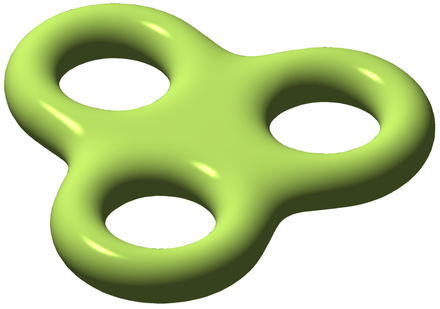
\includegraphics[scale = 1]{RiemannSurface}
**** Riemann Surface of genus 3, from Wikimedia ****

Of course this definition does not apply to curves over fields other than $\CC$, and doesn't relate the genus to the algebra of the curve. However, we can relate the topological genus of a curve directly to its topological Euler characteristic. Since $C$ is topologically compact, connected, and oriented, we have
$H^{0}(C; \ZZ)=H^{2}(C; \ZZ) = \ZZ$, so:
$
\chi_{top}(C) = 2-2g.
$
By the Hopf index theorem, the topological Euler characteristic is the degree of the tangent sheaf, or equivalently, minus the degree of the cotangent sheaf $\omega_{C}$; that is, $\deg K_{C} = 2g-2$, and thus
$$
g(C) = \frac{\deg(K_C)}{2} + 1.
$$
This formula serves to define the genus of a smooth projective curve over any field. 
Other characterizations of the genus require more machinery to establish. We will state some here, and use  tools from the following section to prove equivalence.

\begin{enumerate}

\item 
$
g(C) = 1 - \chi(\cO_C). \label{pa}
$

\item\label{genus Hilbert} If $C \subset \PP^r$ is a smooth curve of degree $d$  with homogeneous coordinate ring
$S_C$, then for sufficiently large $d$ the function $m \mapsto h_C(m) := \dim_\CC (S_C)_m$ is equal to a linear function
$$
p_C(m) =  dm - g + 1,
$$
so $g(C) = dm+1-p_C(m)$. 

\item\label{genus 1forms} $g(C)$ is the dimension of the vector space of regular 1-forms (that is, global sections of the
canonical sheaf) on $C$.
\end{enumerate}

\subsection{Arithmetic genus and geometric genus}
In this section, we'll deal with a  curve $C_0$ that is assumed to be reduced and irreducible.
Any reduced, irreducible 1-dimensional scheme $C_0$ has a normalization $\nu: C \to C_0$ which is a birational
map from a smooth curve. The genus of $C$ is called the \emph{geometric genus} of $C_0$.


The geometry of singular curves is a fascinating topic, from the local analysis of the singularities to the global questions involving linear series on singular curves, and most of the results of this book have analogues for singular curves. But this is a topic beyond the scope of this book; for us, the questions are about smooth curves, with singular curves appearing as a useful adjunct, for example in Chapter~\ref{PlaneCurveChapter}.

Applied to a possibly singular or even non-reduced 1-dimensional projective scheme, the formula~\ref{pa} and the equivalent~\ref{genus Hilbert}, define
what is called the \emph{arithmetic genus} $p_a(C)$. 

We can relate the two notions via the map of sheaves
$$
\cO_{C} \to \nu_*\cO_C.
$$
This is injective; the cokernel sheaf will be a skyscraper sheaf supported exactly on the singular points of $C_0$. Denoting this sheaf by $\cF$, we have an exact sequence
$$
0 \to \cO_{C_0} \to \nu_*\cO_C \to \cF \to 0.
$$

The normalization map $\nu: C \to C_0$ is finite, so that the higher direct images $R^i\nu_*\cO_C = 0$ for $i > 0$; it follows from the Leray spectral sequence that $\chi(\nu_*\cO_C) = \chi(\cO_C)$. Thus
$$
p_a(C_0) - g(C) =  \chi(\cO_{C}) -   \chi(\cO_{C_0}) = \chi(\cF) = h^0(\cF);
$$ 
in other words, the difference between the arithmetic and geometric genera of $C_0$ is the sum of the vector space dimensions of the stalks on $\cF$; colloquially, it's the number of linear conditions a function $f$ on $C$ has to satisfy to be the pullback of a function from $C_0$. The length of the stalk of $\cF$ at a particular singular point $p \in C_0$ is called the \emph{$\delta$-invariant of the singularity}; to rephrase the statement above in these terms, we have
$$
p_a(C_0) - g(C) = \sum_{p \in (C_0)_{sing}} \delta_p
$$ 

The $\delta$ invariant of a singularity is easy to compute in simple cases. For example:
\begin{enumerate}

\item (nodes) If $p \in C_0$ is a node, with points $r,s \in C$ lying over it, the condition for a function $f$ on $C$ to descend is simply that $f(r)=f(s)$; this is one linear condition and accordingly $\delta_p = 1$.

\item (cusps) If $p \in C_0$ is a cusp, with  $r \in C$ lying over it, the condition for a function $f$ on $C$ to descend is simply that the derivative $f'(r)=0$; again, this is one linear condition and accordingly $\delta_p = 1$.

\item (tacnodes) Suppose now that $p \in C_0$ is a \emph{tacnode}, that is, $C_0$ has two smooth branches at $p$ simply tangent to one another. There will be two points $r, s \in C$ lying over it, and the condition for a function $f$ on $C$ to descend is that in terms of suitable local coordinates both $f(r)=f(s)$ and $f'(r)=f'(s)$.  This represents two linear conditions and accordingly $\delta_p = 2$.

\item (planar triple points) Next up, consider an ordinary triple point $p \in C_0$ of a plane curve: that is, a singularity consisting of three smooth branches meeting pairwise transversely, such as the zero locus of $y^3-x^3$. There will be three points $r,s,t \in C$ lying over $p$, and certainly a necessary condition for a function $f$ on $C$ to descend is that $f(r)=f(s)=f(t)$---two linear conditions. But there's a third, less obvious linear condition: in order for $f$ to descend, the derivatives $f'(r), f'(s), f'(t)$ have to satisfy a linear condition---a reflection of the fact that a function on $C_0$ cannot vanish to order 2 on each of two branches without vanishing to order 2 along the third as well. Thus $\delta_p = 3$

\item (spatial triple points) We will be concerned in what follows only with planar singularities, but spatial triple points provide a useful contrast to the last example. A spatial triple point is a singularity consisting of three smooth branches, with linearly independent tangent lines, so that its Zariski tangent space is 3-dimensional. An example would be the union of the three coordinate axes in $\AA^3$.

In this case, in contrast to the last one, the condition that $f(r)=f(s)=f(t)$ is both necessary and sufficient for $f$ to descend, and accordingly we have $\delta_p=2$.

\end{enumerate}

\begin{exercise}
Let $p \in C$ be a singular point of a reduced curve $C$. Show that if $\delta_p = 1$, then $p$ must be either a node or a cusp.
\end{exercise}



\subsection{The Riemann-Roch Theorem}

To prove that these formulas for the genus are correct, we use \trr and Serre duality (sometimes called Kodaira-Serre duality, since Kodaira was responsible for the analytic version.)

\begin{theorem}[Riemann-Roch Theorem]\label{RR}
 If $C$ is a smooth, connected projective curve of genus $g$, and $D$ a divisor of degree $d$ on $C$ then
$$
h^0(D) = d - g + 1 + h^0(K_C - D).
$$
\end{theorem}

For example, if we take $D=0$, this tells us that $h^0(K) = g$, proving the characterization~(\ref{genus 1forms}) above. Using this and \trr for $D=K$
we get $\deg K = 2g-2$. Also, since $h^0(D) = 0$ for any divisor $D$ of negative degree, the formula gives the dimension of $h^{0}(D)$ when $\deg D$ is large:

\begin{corollary}\label{nonspecial RR}
For any divisor $D$ of degree $d$ we have
$$
h^0(D) \geq d - g + 1,
$$
with equality if $d > 2g-2$.
\end{corollary}
This was the theorem originally proven by Riemann; his student Roch supplied the correction term $h^0(K_C - D)$ for divisors of lower degree.
The dimension $h^0(K_C-D) = h^1(D)$ was called the \emph{superabundance} of $D$.

Corollary~\ref{nonspecial RR} and Proposition~\ref{very ample} together show that all high degree divisors come from hyperplane sections in 
suitable embeddings:

\begin{corollary}\label{degree 2g+1 embedding}
Let $D$ be a divisor of degree $d$ on a smooth, connected projective curve of genus $g$. If $d \geq 2g$, the complete linear series $|D|$ is base point free; and if $d \geq 2g+1$ the associated morphism $\phi_D : C \to \PP^{d-g}$ is an embedding, so that
$D$ is the preimage of the intersection of $C$ with a hyperplane in $ \PP^{d-g}$.
\end{corollary}

Since the complement of a hyperplane in projective space is an affine space, we get an affine embedding result too:

\begin{corollary}
 If $C$ is any smooth, connected projective curve and $\emptyset \neq \Gamma \subset C$ a finite subset then $C \setminus \Gamma$ is affine.
\end{corollary}
\begin{proof}
Let $D$ be the divisor defined by $\Gamma$. By Corollary~\ref{degree 2g+1 embedding} a high multiple of $D$ is very ample,
and gives an embedding $\phi: C\to \PP^n$ such that the preimage of the intersection of $C$ with some hyperplane $H$
is a multiple of $D$. It follows that $C\setminus \Gamma$ is embedded in $\AA^n = \PP^n\setminus H$.
\end{proof}
 
We can  use Corollary~\ref{nonspecial RR} to determine the Hilbert polynomial of a projective curve. To do this, let $C \subset \PP^r$ be a smooth curve of degree $d$ and genus $g$, and consider the exact sequence of sheaves
$$
0 \rTo \cI_{C/\PP^r}(m) \rTo \cO_{\PP^r}(m) \rTo \cO_C(m) \rTo 0
$$
and the corresponding exact sequence
$$
 H^0(\cO_{\PP^r}(m)) \rTo^{\rho_m} H^0(\cO_C(m)) \rTo H^1(\cI_{C/\PP^r}(m)) \rTo 0.
$$

The \emph{Hilbert function} $h_C$ of $C$  is defined by
$$
h_C(m) = \dim_{\CC} (S_{C})_{m} = \rank(\rho_m).
$$
By Theorem~\ref{Serre vanishing} we have $H^1(\cI_{C/\PP^r}(m)) = 0$ for large $m$, so $h_{C}(m) = h^0(\cO_C(m))$ for large $m$, which, by the Riemann-Roch theorem, equals $md-g+1$, again for large $m$. Thus, the Hilbert polynomial of $C \subset \PP^r$ is $p_C(m) = dm-g+1$, establishing the characterization~(\ref{genus Hilbert}).
 
The Riemann-Roch formula does \emph{not} give us a formula for the dimension $h^0(D)$ when $h^0(K_C - D)>0$; such divisors $D$ are called \emph{special divisors}, or \emph{special divisor classes}. The existence or non-existence of divisors $D$ with given $h^{0}(D)$ and $h^{1}(D)$ often serves to distinguish one curve from another, and will be an important part of our study.

\begin{fact}
If $k$ is a field that is not algebraically closed there may be smooth projective genus 0 curves over $k$ that are not isomorphic to $\PP^1$. However, they must be ``forms'' of $\PP^1$ in the sense that they become isomorphic to $\PP^1$ after extension of scalars to 
the algebraic closure $\overline k$ of $k$. The unique example with $k = \RR$ is the conic $x^2+y^2+z^2 = 0$. Indeed, any form of $\PP^1$ over any field $k$ can  be embedded in $\PP_{k}^2$  using the anti-canonical linear system.

The curve $\PP_k^1$ itself may be described as the scheme of left ideals of $k$-vector-space dimension 1 in the ring of
$2\times 2$ matrices over $k$ (such an ideal can be embedded in the matrix ring as a linear combination of the 2 columns in an appropriate sense). More generally, any scheme that is a form of $\PP^1$ over $k$
may be described as the scheme of 1-dimensional left ideals in a 4-dimensional central simple ($=$ Azumaya) algebra over $k$. For example, the
conic $x^2+y^2+z^2 = 0$ with no points over $\RR$ is the scheme of left ideals in the algebra of quaternions.\end{fact}

\subsection{A partial proof}

If, following~\ref[Chapter IV]{H} we take the definition of the genus of  a smooth connected curve $C$ to be $h^1(\sO_C)$ (so that $g = h^0(K_C)$ becomes a Corollary of Theorem~\ref{sd}), then it is easy to establish the following form of the Riemann-Roch Theorem:

\begin{corollary}
 If $C$ is a smooth, connected projective curve and $D$ is a divisor on $C$ then
$$
\chi(\sO_C(C)) := h^0(D) - h^1(D) = d-g+1
$$
or in other words, for any invertible sheaf $\cL$ of degree $d$ on $C$,
$$
\chi(\cL) = d-g+1.
$$
\end{corollary}
\begin{proof}
 Taking $D=0$ the statement becomes $h^0(\sO) - h^1(\sO) = 1-g$, which is our definition of $g$. On the other hand,
for any divisor $D$ on $C$ and any point $p \in C$ we have an exact sequence of sheaves
$$
0 \to \cO_C(D-p) \to \cO_C(D) \to \frac{\cO_C(D)}{\gm_{C,p}\cO_C(D)} \to 0
$$
Since $\cO_C(D)$ is locally isomorphic to $\sO_C$ we see that $\cO_C(D)/\gm_{C,p}\cO_C(D)\cong \kappa(p)$ is a sky-scraper sheaf of dimension 1, concentrated at $p$,
and thus has Euler characteristic 1. 
\end{proof}


Thus the Riemann-Roch Theorem for $\cO_C(D)$ is equivalent to the Riemann-Roch Theorem for $\cO_C(D-p)$. Since any divisor can be obtained from 0 by adding and subtracting points, the Riemann-Roch formula for an arbitrary $\cL$ follows from the special case $\cL = \cO_C$.

\subsection{Clifford's theorem}

While the Riemann-Roch Theorem gives a lower bound for the dimension of a linear system, $r(\sL) := h^0(\sL)-1 \geq \deg \sL -g$, Clifford's Theorem
gives an upper bound. If $\deg \sL>2g-2$, then the Riemann-Roch inequality becomes an equality, so it is enough to treat the case $\deg \sL \leq 2g-2$.
To state the sharpest form, we define a curve $C$ of genus $\geq 2$ to be \emph{hyperelliptic} if there exists a $g^1_2$ on $C$; that is an
invertible sheaf $\cL$ of degree $2$ with 2 independent global sections. We will see in Chapter~\ref{genus 2 and 3 chapter} that such a sheaf would be unique, and $h^0(\cL) = 2$.


\begin{theorem}\label{Clifford}
Let $C$ be a curve of genus $g$ and $\cL$ a line bundle of degree $d \leq 2g-2$. Then
$$
r(\cL) \leq \frac{d}{2}.
$$
Moreover, if  equality holds then we must have either
\begin{enumerate}
\item $d=0$ and $\cL = \cO_C$;
\item $d = 2g-2$ and $\cL = K_C$; or
\item $C$ is hyperelliptic, and $|\cL|$ is a multiple of the $g^1_2$ on $C$.
\end{enumerate}
\end{theorem}

\fix{We haven't defined ``hyperelliptic" at this point, or talked about ``the $g^1_2$". Should we just state the weak form of Clifford here, or should we move the definition of hyperelliptic?}

The proof of the inequality will follow easily from a basic result about the addition of linear series, defined as follows:
$\cD = (\cL,V)$ and $\cE = (\cM, W)$ be two linear series on a curve $C$. By the \emph{sum} $\cD + \cE$ of $\cD$ and $\cE$, we will mean the pair 
$$
\cD + \cE = (\cL \otimes \cM, U) 
$$
where $U \subset H^0(\cL \otimes \cM)$ is the subspace generated by the image of $V \otimes W$, under the multiplication/cup product map $H^0(\cL) \otimes H^0(\cM) \to H^0(\cL \otimes \cM)$---in other words, it's the subspace of the complete linear series $|\cL\otimes \cM|$ spanned by divisors of the form $D+E$, with $D \in \cD$ and $E \in \cE$.
 
\begin{proof}
If $\cD$ and $\cE$ are two nonempty linear series on a curve $C$, then
$$
\dim(\cD + \cE) \geq \dim \cD + \dim \cE.
$$
To see this, we observe that to say $\dim \cD \geq m$ means exactly that we can find a divisor $D \in \cD$ containing any given $m$ points of $C$; since $\cD + \cE$ contains all pairwise sums $D + E$ with $D \in \cD$ and $E \in \cE$, we can certainly find a divisor $F \in \cD + \cE$ containing any given $\dim \cD + \dim \cE$ points of $C$.

The proof of the inequality in Clifford's Theorem follows  by applying this observation to the pair $|\cL|$ and $|K_C\otimes \cL^{-1}|$: by 
the Riemann-Roch Theorem, we have
$$
r(K_C\otimes \cL^{-1}) = r(\cL) +g - d - 1
$$
and so we deduce that
$$
g = r(K_C) + 1 \geq r(\cL) + r(K_C\otimes \cL^{-1}) + 1 \geq 2r(\cL) +g - d;
$$
hence $r(\cL) \leq d/2$.

For the proof of the second half of Clifford we will use a basic fact about the geometry of hyperplane sections of a curve in projective space (Proposition~\ref{monodromy of hyperplane section}); we defer it to there.
\end{proof}



\section{The canonical morphism}

Given the central role played by the canonical divisor class, it is natural to look at the geometry of the morphism $\phi_K : C \to \PP^{g-1}$ associated to the complete canonical series $|K|$.  

\begin{definition}
A curve $C$ of genus $g \geq 2$ is said to be \emph{hyperelliptic} if there exists a morphism $f: C \to \PP^1$ of degree 2. \end{definition}

\begin{theorem}\label{canonical system is very ample}
If $C$ is a smooth curve of genus $\geq 2$ then the canonical morphism $\phi_K : C \to \PP^{g-1}$ is an embedding if and only if $C$ is not hyperelliptic.
\end{theorem}

\begin{proof}
By Corollary~\ref{degree 2g+1 embedding} we have to show that for any pair of points $p, q \in C$ we have
$$
h^0(K_C(-p-q)) = h^0(K_C)-2 = g-2.
$$
Applying \trr we see this fails if and only if $h^0(\cO_C(p+q)) \geq 2$ for some $p,q \in C$. By Lemma~\ref{deg 2 morphism}, this implies that $C$ is hyperelliptic.
\end{proof}

\begin{lemma}\label{deg 2 morphism}
Let $C$ be a smooth, projective curve of genus $g\geq 2$. If $C$ has an invertible sheaf $\cL$ of degree 2 with two independent sections, then
$|\cL|$ defines a morphism of degree 2 to $\PP^{1}$, and $C$ is hyperelliptic. In particular, if $g(C) = 2$ then the canonical series $|K_{C}|$ defines a 2 to 1 morphism to $\PP^{1}$, so $C$ is hyperelliptic.
\end{lemma}

\begin{proof}
If $\cO_C(p+q)$ has two independent sections and has $d$ basepoints, then it defines a morphism of degree $2-d$ to $\PP^1$. Since $C$ is not rational,
we must have $d=0$, proving the first statement. 
\end{proof}

\subsection{The geometric Riemann-Roch theorem}

If $C$ is a nonhyperelliptic curve, embedded in $\PP^{g-1}$ by its canonical series and  $D = p_1+\dots + p_d$ is a divisor consisting of $d$ distinct points, let $\overline D$ be the span of the points $p_i \in C \subset \PP^{g-1}$. Since the hyperplanes in $\PP^{g-1}$ containing $\{p_1,\dots,p_d\}$ correspond (up to scalars) to sections of $K_C$ vanishing at all the points $p_i$, we see that
$$
h^0(K_C-D) = g - 1 - \dim \overline D.
$$
Plugging this into the Riemann-Roch formula, we arrive at the statement
$$
r(D) = d - 1 - \dim \overline D;
$$
or in other words, the dimension of the linear series $|D|$ in which the divisor $D$ moves is equal to the number of linear relations on the points $p_i$ on the canonical curve. Thus, for example, if $D = p_1+p_2+p_3$, we see that $D$ moves in a pencil if and only if the points $p_i$ are collinear.

We can extend this statement to the case of arbitrary effective divisors $D$ on any smooth curve if we define our terms correctly. To do this, suppose $f : C \to \PP^d$ is any morphism, and $D \subset C$ any divisor. We define the \emph{span} of  $f(D)$ to be the intersection
$$
\overline{f(D)} = \bigcap_{H \mid f^{-1}(H)\supset D} H 
$$
of all hyperplanes in $\PP^d$ whose preimage in $C$ contains $D$. The argument above applies to prove:

\begin{theorem}[Geometric Riemann-Roch Theorem]\label{geometric RR}
If $C$ is any curve of genus $g \geq 2$,  $\phi : C \to \PP^{g-1}$ its canonical morphism and $D \subset C$ any effective divisor of degree $d$, then
$$
r(D) = d - 1 - \dim \overline{\phi(D)}.
$$
\end{theorem}
 
 \section{Canonical Curves}\label{Noether theorem section}

When we analyze the embedding of a curve $C\subset \PP^n$ we generally ask first whether $C$ is contained in any low-degree
hypersurfaces, and if so how many, in the sense of the dimension $(I_C)_d)$ the degree $d$ part of the homogeneous ideal of $C$.
From the long exact sequence in cohomology
$$
0\to H^0(\sI_{C/\PP^n}(d)) \to H^0(\sO_{\PP^n}(d)) \to H^0(\sO_C(d)) \to H^1(\sI_{C/\PP^n}(d)) \to H^1(\sO_{\PP^n}(d)) \to\cdots
$$
together with the facts that  $H^0(\sO_{\PP^n}(d))$ is the vector space of degree $d$ forms on $\PP^n$ and 
 $H^1(\sO_{\PP^n}(d)) = 0$ for $n>1$ and $d\geq 0$, we see that
 $$
 \dim (I_C)_d = h^0(\sI_{C/\PP^n}(d)) = h^0(\sO_{\PP^n}(d)) - h^0(\sO_C(d)) + h^1(\sI_{C/\PP^n}(d)).
$$
If $d$ times the degree of $C$ is $>2g-2$, the the Riemann-Roch Theorem tell us the value of
 $h^0(\sO_C(d))$, and thus a lower bound for $ \dim (I_C)_d$, but if, in addition, the map
 $H^0(\sO_{\PP^n}(d) \to H^0(\sO_C(d))$ is surjective (or equivalently $h^1(\sI_{C/\PP^n}(d))=0$),
 then we get $ \dim (I_C)_d$ exactly.
 
 
\begin{definition} An embedding of a smooth curve
$C\subset \PP^n$ is said to be \emph{projectively normal} if all the maps $H^0(\sO_{\PP^n}(d)) \to H^0(\sO_C(d))$ are surjective,
or equivalently $h^1(\sI_{C/\PP^n}(d))=0$ for all $d\geq 0$.
\end{definition}
 
By Serre's Criterion of Normality  a 1-dimensional scheme  $C\subset \PP^n$
is a smooth, projectively normal curve iff the homogeneous coordinate ring of $C$ is a normal ring, whence the terminology in
this definition. The criterion has two parts, which are interesting separately: A local or graded ring is normal if it is nonsingular in
codimension 1; and
locally of depth $\geq 2$ in codimension $\geq 2$. In the case of the homogeneous coordinate ring of a curve, 
the first condition means that the curve is nonsingular and the second means that $h^1(\sI_{C/\PP^n}(d))=0$ for all $d$.
In particular, for any very ample invertible sheaf $\sL$ on a smooth curve $C$, the ring 
$$
R(C, \sL) := \bigoplus_{m=0}^\infty H^0(\sL^m)
$$
is normal. See for example \cite[Theorem ***]{Eisenbud1995}.

\begin{example}\label{rnc is projectively normal}
For $d\geq 1$ the rational normal curve $C\subset \PP^d$ of degree $d$ is projectively normal. 
We have $H^0(\sO_{\PP^1}(md))  = \CC[s,t]_{md}$. Th natural natural map
$$
\CC[x_0,\dots,x_d] \to\bigoplus_{m = 0}^\infty H^0(\sO_{\PP^1}(md)));\quad x_0,\dots, x_d \mapsto s^d,s^{d-1}t,\dots, t^d
$$ 
is surjective since every monomial of degree $md$ can be written as a monomial in  
the elements $s^d,s^{d-1}t,\dots, t^d$, and the ring is normal (Exercise~\ref{normality of RNC}).
\end{example}

\begin{exercise}\label{normality of RNC}
 Show that $\CC[s^d,s^{d-1}t,\dots, t^d]$ is normal (ie, integrally closed) by noting that its integral closure must be
 contained in $\CC[s,t]$ and then showing that if $f$ is any polynomial
 in the integral closure then the homogeneous components of $f$ are also in the integral closure.
\end{exercise}


We will now show that the canonical image of a smooth curve is always projectively normal. When the curve is hyperelliptic,
the canonical image is the rational normal curve, treated above, so we may assume that the curve $C$ is embedded
by $|K_C|$ as a smooth curve in $\PP^{g-1}$.


To do this we will make use of an auxiliary construction, a \emph{simple $(g-4)$-secant $(g-3)$-plane.}

\begin{lemma}
 If $C\subset \PP^n$ is a reduced, irreducible, nondegenerate curve, and $m\leq n-1$, then the linear span $L := \overline{p_1,\dots, p_m}$
 of $m$ general points of $C$ is a simple $m$-secant; that is, a plane of dimension $m-1$ such that
 $C\cap L = \{p_1,\dots,p_m\}$ scheme-theoretically.
 \end{lemma}
 
 
\begin{proof}
The plane $L$ is contained in a hyperplane $H$, and since the points are general, we may take this to be a general hyperplane. By Bertini's Theorem, $C\cap H$ is reduced, so $C\cap L$ is also reduced.
 If $C\cap L$ had length $>m$, then by Lemma~\ref{general position lemma} every set of $m+1$ points of $C\cap H$ would be dependent,
 and the span of $C\cap H$ would thus have dimension $\leq m-1<n-1$, and we could choose a hyperplane section $C\cap H'$ with more points than $C\cap H$, which is absurd.
\end{proof}

The following was proven by Max Noether, Emmy's father:

\begin{theorem}[Max Noether]\label{canonical curves are ACM}
A canonical curve in $\PP^{g-1}$ has degree $2g-2$ and arithmetic genus $g$. If the curve has a simple
$g-2$ secant, then it is arithmetically Cohen-Macaulay; that is,
$\HH^{1}(\sI_{C/\PP^{g-1}}(m)) = 0$ for all $m\in \ZZ$.
\end{theorem}
 
For a canonically embedded irreducible curve the simple $g-3$-dimensional $g-2$ secant planes $\Lambda$  correspond to base-point-free pencils of degree $g = 2g-2 -(g-2)$: Given $\Lambda$, the linear series of hyperplanes containing $\Lambda$ intersects $C$ in $\Lambda$ plus the fibers of this pencil. Conversely, given such a pencil, the plane is the span of the complement of a general  member $P$ of the pencil in  $C\cap \overline P$, where $\overline P$ is the hyperplane that is the linear span of $P$.
   
\begin{proof} The Hilbert polynomial $\chi_{C}(t) = h^{0}\sO(t)-h^{1}\sO(t)$ of $C$ has degree equal to
$\dim C = 1$, so it is determined by two values.

We begin by showing that $\sO(-m)$ has no global sections for $m>0$.
If $D$ is a divisor equivalent to $m$ times the hyperplane section, we have an exact sequence
$$
0\to \HH^{0}(\sO_{C}(-m)) \to \HH^{0}(\sO_{C}) \to \HH^{0}(\sO_{D}) \to \cdots.
$$
By hypothesis, the vector space $\HH^{0}\sO_{C}$ is spanned by the constant functions, and these
restrict non-trivially to $\sO_{D}$, and $\HH^{0}(\sO_{C}(-m)) = 0$ as claimed.

Using the Riemann-Roch Theorem we can now compute the Hilbert function $\chi_{C}(m)$:
We have 
\begin{align*}
 \chi_{C}(0) &= h^{0}(\sO_{C}) - h^{1}(\sO_{C}) = h^{0}(\sO_{C}) - h^{0}(\omega_{C}) = 1-g.\\
\chi_{C}(1) &= h^{0}(\sO_{C}(1)) - h^{1}(\sO_{C}(1)^{*}\otimes \omega_{C}) = h^{0}(\omega_{C}) - h^{0}(\sO_{C}) = g-1.
\end{align*}
and we deduce
$\chi_{C}(m) = (2g-2)m -g+1$, whence we see that the degree of $C$ is $2g-2$ and $p(C) = g$ as claimed.

To show that
$C$ is arithmetically Cohen-Macaulay we use the sequence
$$
\cdots \to \HH^{0}(\sO_{\PP^{n}}(m)) \to \HH^{0}(\sO_{C}(m))
\to \HH^{1}(\sI_{C}(m))\to \HH^{1}(\sO_{\PP^{n}}(m)) \to\cdots .
$$
Since $\HH^{1}(\sO_{\PP^{n}}(m)) = 0$, it
is enough to show that the natural map 
$$
\HH^{0}(\sO_{\PP^{n}}(m)) \to \HH^{0}(\sO_{C}(m))
$$
 is surjective for all $m\in \ZZ$. For $m=0,1$ this is immediate from the hypothesis.

For $m <0$ we must show $\HH^{0}(\sO_{C}(m))=0.$ 
If $D$ is a divisor equivalent to $-m$ times the hyperplane section, we have an exact sequence
$$
0\to \HH^{0}(\sO_{C}(m)) 
\to \HH^{0}(\sO_{C}) 
\to \HH^{0}(\sO_{D}) \to \cdots.
$$
By hypothesis, the vector space $\HH^{0}\sO_{C}$ is spanned by the constant functions, and these
restrict non-trivially to $\sO_{D}$, so the kernel, $\HH^{0}(\sO_{C}(m))$, is 0 as claimed. 

To prove surjectivity for $m\geq 2$ we use the remaining hypothesis, the existence of
a simple $g-3$-dimensional $g-2$ secant plane $\Lambda$  and an idea sometimes called the \emph{base-point-free pencil trick}. Let $p_{0},\dots p_{g-3}$ be the points in which $\Lambda$ meets $C$.  Since the
$p_{i}$ are linearly independent by hypothesis, we may choose homogeneous coordinates $x_{i} \in \HH^{0}(\sO_{C}(1))$ so that
$x_{i}(p_{j}) \neq 0$ if and only if $i = j$. It follows that the sections
$x_{i}^{m}$ of $\sO_{C}(m)$ span $\HH^{0}(\sO_{C}(m)|_{\{p_{0}, \dots, p_{g-3}\}})$. Let 
$V\subset \HH^{0}(\sO_{C}(1))$ be the two-dimensional subspace of linear forms vanishing on
$\Lambda$, and thus on the $p_{i}$. 

For $m\geq 2$ there are maps of vector spaces
$$
\wedge^{2} V\otimes \HH^{0}(\sO_{C}(m-2)) \to V\otimes \HH^{0}(\sO_{C}(m-1)) 
\to \HH^{0}(\sO_{C}(m))
$$
where the right hand map is multiplication and the left hand map sends
$s_{1}\wedge s_{2}\otimes \sigma$ to $s_{1}\sigma-s_{2}\sigma$ for any local section $\sigma$.
The sequence is exact because the sections $s_{1},s_{2}$ that span $V$ never vanish simultaneously except on the $p_{i}$, and has image  consisting of sections that vanish on the points $p_{i}$

\end{proof}

\begin{corollary}\label{canonical hilbert function}
If $C\subset \PP^{g-1}$ is a canonical curve with a simple $g-3$-secant, then the Hilbert function of the homogeneous coordinate ring $S_{C}$ of  $C$ depends only on $g$, and is given by:
$$
\dim({S_{C}})_{d} = h^{0}(\cO_{C}(d)) = 
\begin{cases}
 0 &\mbox {if } d<0\\
 1 & \mbox {if }  d=0\\
 g & \mbox {if }  d=1\\
 (2n-1)g+1 & \mbox {if }  d>1\\
\end{cases}
$$
\end{corollary}
\begin{proof}
Theorem~\ref{canonical curves are ACM} implies, in particular, that the homogeneous coordinate ring of $C$ can be identified with 
$\oplus_{n\in \ZZ}\HH^0\sO_C(n)$.  
\end{proof}

 \section{A bit about surfaces}
 We will often analyze curves  on a smooth surface; here are a few results that will be useful. We refer to~\cite[Chapter V]{Hartshorne1977}
 and~\cite[Chapter I]{Beauville} for proofs.
 
 We suppose for this section that $X$ is a smooth projective surface.
 We define $\Pic(X)$ to be the group whose elements are invertible sheaves on $X$.
When two divisors $D,E$ on $X$ meet transversely we define $D\cdot E$ to be the number of points in which they meet. If they have no common
components, we can still define a non-negative intersection multiplicity $m_X(D,E,p)$ at each point $p$, and then set
$$
D\cdot E = \sum_p m_X(D,E,p).
$$
Over the complex numbers each codimension 1 subvariety $D$ of $X$ has a fundamental class
$[D]\in H^2(X, \ZZ)$ and the product is the cup product with values in $H^4(X,\ZZ)$, which is $\ZZ$ since $X$ is compact and orientable. Thus
there is an extension of the product to the cases where $D,E$ have common components. From a geometric point of view, we may choose an
appropriate $C^\infty$
normal vector field along $E$ and define $E'$ by ``pushing'' $E$ out slightly along the direction of this field, until $D$ and $E'$ are transverse,
and the intersections can be computed in the usual way. It should be noted that such intersection numbers can be either positive or negative,
since they depend on the relative orientations of $D$ and $E'$ at the intersection points; this is in contrast to the case when $D$ and $E$
themselves meet properly; in this case the fact that the complex numbers are canonically oriented makes the intersection number non-negative.

The intersection product can also be defined algebraically, over any field: Setting $\sL := \sO_X(C)$ and
$\sM := \sO_X(D)$ to simplify the notation, we set 
$$
D\cdot E = \chi(\sO_X)-\chi(\sL^{-1}) -\chi(\sM^{-1}) -\chi(\sL^{-1}\sM^{-1}) 
$$
\begin{theorem} The pairing $(D,E) \mapsto (D.E)$ is the unique bilinear map
$\Pic(X) \times \Pic(X) \to \ZZ$ extending the case of intersections of two transverse curves on $X$. 
\end{theorem}

A frequent use of the the intersection pairing is to compute the (arithmetic) genus of a curve on a surface,
a result called the adjunction formula.

\begin{theorem}[Adjunction Formula]\label{adjuction formula}
If $C$ is a curve lying on a smooth surface $X$ then 
$$
\omega_C = \omega_X \otimes \sO_X(C) \otimes \sO_C.
$$
In particular \label{genus formula}
$$
p_a(C) = \frac{(K_X+C)\cdot C}{2} +1
 $$
\end{theorem}

We will frequently be interested in curves on quadrics in $\PP^3$, and we can spell out the
intersection theory on these surfaces very concretely; see for example~\cite[****]{Hartshorne1977}.
We will treat them and the curves on them in detail in Section~\ref{curves on scrolls} as part of the larger family of 2-dimensional rational normal scrolls; for
now we sketch the situation as an example of the theory of this section. 

\begin{example}[Quadrics in $\PP^3$]\label{Div of quadric}
 
Quadric surfaces $S$ in $\PP^3$ are classified by their rank:
\begin{itemize}
\item A quadric of rank 2 is the union of two planes; it cannot contain an nondegenerate irreducible curve
\item A rank 3 quadric $S$ is a cone over a plane conic. Suppose that $C$ is a smooth,
curve on such a quadric:
\begin{itemize}
\item  If $C$  does
not pass through the vertex then it is the intersection of the quadric with a hypersurface of some
degree $d$. In this case $C$ has degree $2d$ and genus $(d-1)^2$. 
 \item if $C$ passes through the vertex, then $C$ lies in the divisor class of a line through the origin plus the intersection of $S$ with a hypersurface of some degree $d$. In this case $C$ has degree $2d+1$ and 
 genus $d(d-1)$. 
\end{itemize}

%If  it contains smooth irreducible curves that do not pass through the vertex of the cone, and smooth irreducible curves that of
%degree $2d$ that are intersections of $S$ with hypersurfaces of degree $d$; and smooth 
%irreducible curves of degree $2d+1$ that 

\item A quadric of rank 4 is nonsingular, and is isomorphic to $\PP^1\times \PP^1$.


\item The Picard group of $\PP^1\times \PP^1$ is $\ZZ\oplus \ZZ$, generated by the 
classes of the lines $\{p\}\times \PP^1$ and $\PP^1\times \{p\}$, where $p\in \PP^1$
is any point. These lines have self-intersection 0, and meet transversely in a point,
so the intersection pairing is given by $(a,b)\cdot(c,d) = ad+bc$. From the adjunction formula
applied to the classes of the lines $(1,0)$ and $(0,1)$ we that the canonical
class is $(-2,-2)$, and thus the arithmetic genus of a curve of type $(a,b)$ is thus
$$
\left(((a,b)+(-2,-2))\cdot (a,b)\right)/2 +1 = (a-1)(b-1).
$$

\item Writing $\pi_1, \pi_2$ for the two projections of
$\PP^1\times \PP^1 \to \PP^1$, the sheaf 
$$
\sL := \sO_{\PP^1\times \PP^1}(a,b) = \pi_1^*\op1a \otimes \pi_2^*\op1b
$$
has cohomology given by the K\"unneth formula, for example
\begin{align*}
 H^0(\sL) &= H^0(\op1a)\otimes H^0(\op1b) \hbox{ and thus }\\
 h^0(\sL) &= (a+1)(b+1) \hbox{ if } a\geq 0, b\geq 0.
\end{align*}

\item Any smooth quadric surface $S\subset \PP^3$ is the 
image of $\PP^1\times \PP^1$ embedded by the complete linear system
$|\sO_{\PP^1\times \PP^1}(1,1)|$ and thus contains two families of lines. 
A curve in the class $(a,b)$ thus has degree $(a,b)\cdot(1,1) = a+b$. 
\end{itemize}
\end{example}

Often we wish to compute the dimension of the space of sections of an invertible sheaf, but
as with the case of curves, the Euler characteristic is more accessible:

\begin{theorem}[Riemann-Roch for surfaces] Let $\sL$ be an invertible sheaf on a smooth surface $S$.
the Euler characteristic $\chi(D) := h^0(\sL)-h^1(\sL)+h^2(\sL)$, where $\sL = \sO_S(D)$, is given by
$$
\chi(D) = \chi(\sO) + \frac{(D-K_S)\cdot D}{2}+1
$$
\end{theorem}

\fix{Possible addition:  the Hodge Index theorem as corollary. This could be used to prove finiteness of the automorphism group of a curve following Hartshorne V Ex. 1.11, perhaps in place of the proof now in the inflections chapter.}

It is useful to know what happens under mappings of surfaces, particularly the case of the mapping
corresponding to blowing up a point.

\begin{theorem}
If $\pi: X \to Y$ is a birational map of smooth surfaces, then the pullback map on divisors
preserves the intersection pairing. If $X$ is the blowup of $Y$ at a point $p$, with exceptional
divisor $E = \pi^{-1}(p)$ then:

\begin{enumerate}
 \item $\Pic X =\pi^*(\Pic Y) \oplus \ZZ E$.
\item The canonical class on $X$ is given by $K_X = \pi^*(K_Y)+E$.
 \item The intersection pairing on $\Pic X$ is given by
 
\begin{itemize}
\item $\pi^*(D)\cdot\pi^*(D') = D.D'$ for all $D,D'\in \Pic Y$.
\item $\pi^*(D)\cdot E = 0$ for all $D\in \Pic Y$.
 \item $E\cdot E = -1$.
 \item $K_X\cdot E = -1$.
 \item If $C$ is a curve that has an $m$-fold point at $p$ then $\pi^{-1}(C)$ contains $E$ with multiplicity $m$.
 \end{itemize}
\end{enumerate}
\end{theorem}

Blowups occur frequently in the theory of surfaces, and are easy to characterize:
\begin{theorem}
If $E\subset X$ is a curve on a smooth projective surface $X$ and
 that $E^2 = E\cdot K_X = -1$ then $E$ can be ``blown down'' in the sense that
 $X$ is the blowup of a smooth surface $Y$ at a point $p\in Y$, and $E$ is the exceptional divisor.
\end{theorem}


\input footer.tex
%header and footer for separate chapter files

\ifx\whole\undefined
\documentclass[12pt, leqno]{book}
\usepackage{graphicx}
\input style-for-curves.sty
\usepackage{hyperref}
\usepackage{showkeys} %This shows the labels.
%\usepackage{SLAG,msribib,local}
%\usepackage{amsmath,amscd,amsthm,amssymb,amsxtra,latexsym,epsfig,epic,graphics}
%\usepackage[matrix,arrow,curve]{xy}
%\usepackage{graphicx}
%\usepackage{diagrams}
%
%%\usepackage{amsrefs}
%%%%%%%%%%%%%%%%%%%%%%%%%%%%%%%%%%%%%%%%%%
%%\textwidth16cm
%%\textheight20cm
%%\topmargin-2cm
%\oddsidemargin.8cm
%\evensidemargin1cm
%
%%%%%%Definitions
%\input preamble.tex
%\input style-for-curves.sty
%\def\TU{{\bf U}}
%\def\AA{{\mathbb A}}
%\def\BB{{\mathbb B}}
%\def\CC{{\mathbb C}}
%\def\QQ{{\mathbb Q}}
%\def\RR{{\mathbb R}}
%\def\facet{{\bf facet}}
%\def\image{{\rm image}}
%\def\cE{{\cal E}}
%\def\cF{{\cal F}}
%\def\cG{{\cal G}}
%\def\cH{{\cal H}}
%\def\cHom{{{\cal H}om}}
%\def\h{{\rm h}}
% \def\bs{{Boij-S\"oderberg{} }}
%
%\makeatletter
%\def\Ddots{\mathinner{\mkern1mu\raise\p@
%\vbox{\kern7\p@\hbox{.}}\mkern2mu
%\raise4\p@\hbox{.}\mkern2mu\raise7\p@\hbox{.}\mkern1mu}}
%\makeatother

%%
%\pagestyle{myheadings}

%\input style-for-curves.tex
%\documentclass{cambridge7A}
%\usepackage{hatcher_revised} 
%\usepackage{3264}
   
\errorcontextlines=1000
%\usepackage{makeidx}
\let\see\relax
\usepackage{makeidx}
\makeindex
% \index{word} in the doc; \index{variety!algebraic} gives variety, algebraic
% PUT a % after each \index{***}

\overfullrule=5pt
\catcode`\@\active
\def@{\mskip1.5mu} %produce a small space in math with an @

\title{Personalities of Curves}
\author{\copyright David Eisenbud and Joe Harris}
%%\includeonly{%
%0-intro,01-ChowRingDogma,02-FirstExamples,03-Grassmannians,04-GeneralGrassmannians
%,05-VectorBundlesAndChernClasses,06-LinesOnHypersurfaces,07-SingularElementsOfLinearSeries,
%08-ParameterSpaces,
%bib
%}

\date{\today}
%%\date{}
%\title{Curves}
%%{\normalsize ***Preliminary Version***}} 
%\author{David Eisenbud and Joe Harris }
%
%\begin{document}

\begin{document}
\maketitle

\pagenumbering{roman}
\setcounter{page}{5}
%\begin{5}
%\end{5}
\pagenumbering{arabic}
\tableofcontents
\fi


\chapter{The Riemann--Roch theorem}\label{RiemannRochChapter}

\section{How many sections?}

To study curves via their maps to projective spaces, we want to estimate the dimension of the space of global
sections of an invertible sheaf $\cL$. The beginning
of the story is the Riemann--Roch theorem.

Though we would like to be able to compute $h^0(\sL)$, it is much
easier to compute the 
\blue{Euler characteristic}
\index{Euler characteristic}%
$$
\chi(\sL):= \sum_{i\geq 0} (-1)^i h^i(\sL).
$$
This computes $h^0(\cL)$ itself in many cases, by virtue of the following result:
\marginpar{indexed theorem name}

\begin{theorem}[Serre--Grothendieck vanishing theorem]
\label{Serre--Grothendieck vanishing}
\index{Serre--Grothendieck vanishing theorem}%
\index{vanishing theorem!Serre--Grothendieck}%
If $\sF$ is a coherent sheaf on a projective scheme $X$ of dimension $n$, then for any $i$, the vector space $H^i(\sF)$ is finite-dimensional, and is 0 if  $i> n$. Moreover,
if $X\subset \PP^m$ then for $d\gg 0$, $\sF(d)$ is generated by its global sections and $H^i(\sF(d)) = 0$ for all $i>0$.\qed
\end{theorem}

\begin{proof}
This is a combination of 
theorems due to Grothendieck and Serre. See
\cite[Theorems III.2.7 and III.5.2]{Hartshorne1977}, 
and
also \cite{Serre1955} for a 
reasonably
concrete proof.
\end{proof}

A 
shortcoming
of this vanishing theorem is the lack of a bound on the number $d$ needed to achieve the second assertion. For smooth curves
and invertible sheaves
this is corrected by Theorem~\ref{RR theorem}, which gives a bound in terms of the genus and the degree.

One immediate consequence of Theorem~\ref{Serre--Grothendieck vanishing} is that on a smooth variety the groups of invertible sheaves and divisor classes are the same:

\begin{corollary}\label{invertible sheaves and divisors}
If $X$ is a projective variety that is nonsingular in codimension $1$,
every invertible sheaf $\cL$ on $X$ is of the form $\cL =\cO_C(D)$ for some 
\index{Cartier divisor}\index{divisor!Cartier}%
Cartier divisor $D$ on $X$. Thus if $X$ is a smooth projective variety
\index{notation!div}%
the map $\div$ is an isomorphism from the group of invertible sheaves
to the group 
of divisor classes.
\end{corollary}

\begin{proof}
Let $H \subset \PP^r$ be a general hyperplane, and $E$  the divisor  of intersection of $C$ with $H$. We know that for $n \gg 0$, $\cL(n)$ has sections; and if $F$ is the divisor of zeroes of one such section, we have
$$
\cL = \cO_C(F - nE).
$$
If $X$ is smooth, then, since a regular local ring is a unique
factorization domain, every codimension-one subvariety is defined locally 
by a single nonzerodivisor, and thus corresponds to a Cartier divisor.
This implies that $\div$ is surjective. Furthermore any 
\blue{isomorphism between invertible sheaves}
\index{invertible sheaf!isomorphism between -s}%
is defined by multiplication with a global rational function, so that invertible sheaves defining linearly equivalent divisors are
isomorphic. Thus $\div$ is injective as well.
\marginpar{(de): this proof is pretty swift, and the result fundamental. Let's give a Hartshorne citation too.}
\end{proof}

\subsection*{Riemann--Roch without duality}

It follows from Theorem~\ref{Serre--Grothendieck vanishing} that on
any scheme $X\subset \PP^r$ we have $\chi(\sL(d)) = h^0(\sL(d))$ for
large $d$, 
and that $\chi(\sL) = h^0(\sL) - h^1(\sL)$ in the case of a curve.

\begin{theorem}[easy Riemann--Roch]\label{easy RR}
If $C$ is a smooth projective curve, and $\sL$ is an invertible sheaf on $C$, then $\chi(\sL) = \deg \sL + \chi(\sO_C)$.
\index{Riemann--Roch theorem!easy}%
\end{theorem}

\begin{proof}
 The result is tautological if $\sL = \sO_C$. Every invertible sheaf on $C$ has the form $\sL = \sO_C(D)$ for some
divisor $D$. If $p\in C$, then writing $\kappa(p)$ for the
structure sheaf of the subscheme $p\in C$, the long exact sequence in cohomology
associated to the short exact sequence
$$
0\to \sL(-p) \to \sL \to \sL\otimes \kappa(p)\to 0
$$
together with the isomorphism $\sL\otimes \kappa(p) \cong \kappa(p)$
and the vanishing of higher cohomology of a sheaf with zero-dimensional support allows us to compute 
$$
\chi(\sL) = \chi(\sL(-p)) + \chi(\kappa(p)) = \chi(\sL(-p)) + 1.
$$
Since every divisor on $C$ can be reached by adding and subtracting points, this suffices.
\end{proof}

Since the Euler characteristic of a sheaf is well-behaved, we can extend the result of Theorem~\ref{easy RR} 
to invertible sheaves on any one-dimensional scheme $C$, by defining
$\deg \sL := \chi(\sL) -\chi(\sO_C)$.
We will use this definition to express the self-intersection of a divisor on a surface in Section~\ref{surface basics}.

We can make the Riemann--Roch theorem still more useful by understanding the error term $h^1(\sL)$. This requires
the canonical divisor and Serre duality, to which
we now turn.


\section{The most interesting linear series}\label{most interesting}

The most important vector bundles on a manifold are the tangent and cotangent bundles. For reasons that
will become clear, the focus in algebraic geometry is on the cotangent
bundle or, equivalently, the sheaf of differential 1-forms. On a
smooth curve $C$ the \emph{canonical sheaf} is the sheaf of
differentials, which is an 
\index{canonical sheaf}\index{sheaf!canonical}\index{sheaf!of differentials}%
invertible sheaf; on a smooth
variety of dimension $n$ we define the canonical sheaf to be the 
$n$-th exterior power of the sheaf of differentials. A section of 
$\omega_C$ is thus a differential form, and the class of the divisor
of such a form is usually denoted 
\blue{$K_C$.}
\index{notation!$K_C$}%

\begin{fact}
Canonical sheaves are defined for any projective scheme; see 
Definition~\ref{dualizing sheaf for singular curve}.
They are usually called 
\index{dualizing sheaf}\index{sheaf!dualizing}%
{\it dualizing sheaves} 
in that generality. The condition for the dualizing sheaf to be an invertible
\index{Gorenstein scheme}%
sheaf is that the scheme is (locally) Gorenstein, something that is true, for example, for any subscheme of $\PP^r$
that is locally a complete intersection (see Section~\ref{dualizing sheaves section}).
\end{fact}
 

On projective space we can compute the canonical sheaf directly; other computations of the canonical sheaf will usually reduce to this central case.

\begin{theorem}
 The 
\blue{canonical sheaf of $\PP^{r}$}
\index{canonical sheaf!of $\PP^{r}$}%
is $\sO_{\PP^{r}}(-r-1)$. 
\vspace*{-\parskip}
\end{theorem}

\begin{proof}
Let $x_{0}, \dots, x_{r}$ be the projective coordinates on $\PP^{r}$
and let  $U = \PP^{r}\setminus H$ be the affine open set where $x_{0}
\neq 0$. Thus $U \cong \AA^{r}$ with coordinates $z_{1} :=
x_{1}/x_{0}$, $\dots$, $z_{r}:=x_{r}/x_{0}$. The space of
$r$-dimensional differential forms on $U$ is spanned by
$d(x_{1}/x_{0})\wedge\cdots\wedge d(x_{r}/x_{0})$, which is regular
everywhere in $U$. In view of the formula
$$
d\frac{x_{i}}{x_{0}} = \frac{x_{0}\,dx_{i}-x_{i}\,dx_{0}}{x_{0}^{2}}
$$
we get
$$
d\frac{x_1}{x_0}\wedge\cdots\wedge 
d\frac{x_r}{x_0}
= \frac{dx_{1}\wedge\cdots\wedge dx_{r}}{x_{0}^{r}}-
\sum_{i=1}^{r} x_{i} \frac{ dx_{1}\wedge\cdots \wedge \widehat{dx_{i}}\wedge \cdots \wedge dx_{r}}{x_{0}^{r+1}}
$$
which has a pole of order $r+1$ along the locus $H$ defined by $x_{0}$. Thus the divisor of this differential form
is $-(r+1)H$, and this is the canonical class.
\end{proof}

\begin{fact}
A different derivation: there is a short exact sequence of sheaves,
\index{Euler sequence}%
\marginpar{Ch. II $\to$ II (or else Chapter II, \S8 if you feel it's safer)}
called the Euler sequence \cite[II.8]{Hartshorne1977}:
$$
0\to \Omega_{\PP^{r}} \to \sO_{\PP^{r}}^{r+1} (-1) \to \sO_{\PP^{r}} \to 0.
$$
Summing over all twists, and taking global sections, that is, applying $H^0_*$, we see that 
$H^0_*(\Omega_{\PP^{r}})$ fits into an exact sequence:
$$
0 \to H^0_*(\Omega_{\PP^{r}}) \to S^{r+1}(-1) \ruto{\delta_{1}} S \to \CC \to 0,
$$
where $S$ is the homogeneous coordinate ring of $\PP^r$ and $\delta_1$ sends the $i$-th basis vector of
$S^{r+1}(-1)$ to the $i$-th variable of $S$; that is, $H^0_*(\Omega_{\PP^{r}})$ is the second syzygy of the residue field $\CC$ of $S$. We can extend this sequence to the Koszul complex that is the free resolution
of $\CC$, 
\index{Koszul complex}%
\cite[\S17.5]{Eisenbud1995}:
$$
0 \to S(-r-1) \ruuto{\delta_{r+`1}} 
\mwedge^rS^{r+1}(-r) \ruto{\delta_{r}} \cdots \to S^{r+1}(-1) \to S \to \CC \to 0.
$$
For each $i$, the $i$-th exterior power of the map $H^0_*(\Omega_{\PP^{r}}) \to S^{r+1}(-1)$ is an inclusion, and
represents $\mwedge^i(\Omega_{\PP^{r}})$ as the sheaf associated to the graded module that is the $(i+1)$-st syzygy of $\CC$.
In particular, the canonical module $\omega^{}_{\PP^r} = \mwedge^r(\Omega_{\PP^{r}})$ is the sheaf associated to the 
$(r+1)$-st syzygy, $S(-r-1)$.

For more on syzygies, see Chapter~\ref{SyzygiesChapter}.
\end{fact}

The most important invariant of a smooth curve can be defined in terms of the canonical sheaf:

\begin{definition}
If $C$ is an irreducible smooth curve we define the genus $g(C)$ to be the dimension of $H^0(\omega_C)$.
\end{definition}

Computations of the canonical sheaf on a variety usually involve
comparing the variety to a variety 
whose
canonical sheaf is already known. The most useful results of this type
are  the \emph{adjunction formula}
and \emph{Hurwitz's theorem}. 

\subsection*{The adjunction formula}%\label{Adjunction Formula}

In the simplest case, the adjunction formula says that the canonical divisors of a smooth plane 
curve $C$ of degree $d$ are the intersections of $C$ with curves of degree $d-3$ 
(see Figure~\ref{canonical of quartic}). 
More generally, for a divisor $X$ on a smooth variety $Y$, it says that
the canonical sheaf on $X$ is $\omega_Y(X)|_X$. This is an immediate consequence of
the still more general formula below because the normal bundle of $X$ is $\sO_Y(X)$.

In general, the adjunction formula describes the difference between the canonical divisor of
a  subscheme and the restriction of the canonical divisor from the ambient variety.
If $X\subset Y$ we define the \emph{conormal sheaf} of $X$ in $Y$ to be $\sI_{X/Y}/\sI_{X/Y}^{2}$,
and the \emph{normal sheaf} of $X$ in $Y$ to be its dual, 
$$
\sN_{X/Y} = \sHom(\sI_{X/Y}/\sI_{X/Y}^{2}, \sO_{Y}).
$$
If $X$ and $Y$ are smooth, $X$ is locally a complete intersection in $Y$, so
 $@\sI_{X/Y}/\sI_{X/Y}^{2}$ 
is a vector bundle on $X$ of rank equal to the codimension, $\dim Y -\dim X$.
 When, in addition, the codimension is 1, so that $X$ is a divisor and $\sI_{X} = \sO_{Y}(-X)$, we get
 $$
 \sN_{X/Y} = \sO_{X}(X).
 $$


\begin{proposition}[adjunction formula]\label{adjunction}
 Let $X\subset Y$ a smooth subscheme of codimension $c$ in a smooth variety $Y$, and let $K_{Y}$ be the canonical class of $Y$. The canonical class $K_X$ of $X$ is 
\index{adjunction formula}\index{formula!adjunction}%
 $$
 \omega_{X} = \mwedge^{c} \sN_{X/Y} \otimes \omega_{Y}.
 $$
In particular, when $X$ is a divisor, $K_{X}$ is the restriction to $X$ of the divisor $K_{Y}+X$ on $Y$.
\end{proposition}

\begin{figure}
\centerline{\includegraphics[width=2.5in]{"main/Fig02-1"}}
\caption{On a smooth plane quartic, the canonical divisors are its
  intersections with lines.
}\label{canonical of quartic}
\end{figure}


\begin{proof}
 Because $X$ is locally a complete intersection in $Y$ there is an exact sequence of sheaves
 $$
0\to  \sI_{X/Y}/\sI_{X/Y}^{2} \to \Omega_{Y}| _{X} \to \Omega_{X} \to 0
,
 $$
 where $\Omega_{X}$ is the sheaf of differential forms on $X$ (see \cite[Proposition 16.3]{Eisenbud95}), and
$ \sI_{X/Y}|_{X} = \sO_{Y}(-X)|_{X} = \sO_{X}(-X)$. The proposition follows by taking top exterior powers, 
as in Lemma~\ref{exterior powers}.\end{proof}

\begin{lemma}\label{exterior powers}
 If 
$$
0\to \sE \to \sF\to \sG \to 0
$$
is a short exact sequence of locally free sheaves of ranks $e,f,g$ 
 on a scheme $X$, then there is a natural
isomorphism 
$$
\mwedge^e\sE \otimes \mwedge^g \sG \to \mwedge^f\sF.
$$
\end{lemma}

\begin{proof}[Proof of Lemma~\ref{exterior powers}]
 We may define a map
$
\mwedge^e\sE \otimes \mwedge^g \sG \to \mwedge^f\sF
$
in terms of local sections as
$$
(\epsilon_1\wedge\cdots \wedge \epsilon_e) \otimes (\gamma_1\wedge\cdots\wedge \gamma_g)
\mapsto \epsilon_1\wedge\cdots \wedge \epsilon_e\wedge\gamma_1\wedge\cdots\wedge \gamma_g.
$$
This is globally well-defined because changing one of the $\gamma_i$ by a local section of $\sE$ would not
change the exterior product.
To check that the map is an isomorphism, it is enough to show that this is true locally.

Because $\sG$ is locally free, there is a covering of $X$ by open sets $U$
so that the sequence
$$
0\to \sE|_U \to \sF|_U\to \sG|_U \to 0
$$
is a split exact sequence of free modules, $\sF|_U = \sE|_U\oplus \sG|_U$.
It follows that
$$
\mwedge^f\sF|_U = 
\tsty\bigoplus\limits_{i+j = f} \mwedge^i \sE|_U \otimes \mwedge^j\sG|_U.
$$
In our case all the exterior powers of $\sE$ vanish above the $e$-th, and all the 
exterior powers of $\sG$ vanish above the $g$-th, so 
$$
\mwedge^f\sF|_U =  \mwedge^e \sE|_U \otimes \mwedge^g\sG|_U,
$$
with isomorphism given as above.
\end{proof}


\begin{corollary}\label{canonical of plane curve}\label{canonical of complete intersection}
If $C\subset \PP^{2}$ is a smooth plane curve of degree $d$, then
$\omega_{C} = \sO_{C}(d-\nobreak 3)$; more generally, if
$X\subset \PP^{r}$ is a smooth complete intersection of hypersurfaces of degrees $d_{1},\dots, d_{c}$ in $\PP^r$ then
$\omega_{X} = \sO_{X}(\sum d_{i }-r-1).$
\vspace*{-3pt}
\end{corollary}

\begin{proof}
Since $\sN_{X/Y} = \bigoplus\limits_{i=1}^{c} \sO_{X}(d_{i})$, the result follows from Theorem~\ref{adjunction}.
\end{proof}

\subsection*{Hurwitz's theorem}
 Given a (nonconstant) morphism $f : C \to X$ of smooth projective
 curves, the Riemann--Hurwitz formula computes the canonical sheaf
 $C$ in terms of that of  $X$ and the local geometry of $f$. To do
 this we define the
\index{Hurwitz's theorem}\index{theorem!of Hurwitz}%
\index{Riemann--Hurwitz formula}\index{formula!Riemann--Hurwitz}%
\index{ramification index}%
\blue{\emph{ramification index}}%
of $f$ at $p \in C$,  denoted $\ram(f,p)$, 
by the formula 
$$
 f^{-1}(q) = \!\sum_{\substack{\,p\in C\\ f(p)=q}}\! (\ram(f,p)+1)\cdot p
 $$
 for any point $q \in X$. 

\begin{proposition}
If $f : C \to X$ is a (nonconstant) morphism  of smooth projective curves,
there are only finitely many
points $p\in C$ such that $\ram(f,p)>0$.
\end{proposition}

In light of this result we define the \emph{ramification divisor}
\index{ramification divisor}% 
of $f$ to be the divisor
 $$
 R = \sum_{p \in C} \ram(f,p)\cdot p \; \in \;  \Div(C).
 $$
 and the \emph{branch divisor} to be
 $$
 B = \sum_{q \in X} \Big(\sum_{p \in f^{-1}(q)} \ram(f,p) \Big)\cdot q \; \in \; \Div(X).
 $$
Note that $R$ and $B$ have the same degree, which is $\sum_{p \in C} \ram(f,p)$.

\begin{proof}
The result follows from the separability of the map of fields of rational functions, $K(X) \to K(C)$, which holds because we
are in characteristic 0 (in characteristic $p$ the 
\blue{Frobenius map}
\index{Frobenius map}%
provides a counterexample). A proof using separability
is given in~\cite[Section IV.2]{Hartshorne1977}. Here is an analytic version:

In terms of local parameters $z$ on $C$ around $p$ and $w$ on $X$ around $f(p)$, we can write the morphism as $z \mapsto w = z^m$ for some integer $m > 0$; that is,
if $w$ is a local parameter on $X$ and $z$ is a local parameter in the source, then
the map
$$
 \CC\{` `\{w\}` `\} \cong \widehat\sO_{X,f(p)} \ruto{\hat f^*}\widehat\sO_{C,p}\cong  \CC\{` `\{z\}` `\} 
$$ 
of convergent power series rings induced by $f^*$
sends $w$ to $uz^m` `$, where $u$ is a power series with nonvanishing constant term.
In this case $\ram(f,p) = m-1$. These power series expansions are valid in a neighborhood
of $p$, and the derivative of $f$ vanishes at the ramification points in this neighborhood. Since
the zeros of a nonconstant analytic function are isolated, the ramification points are isolated. 
Since $C$ is compact in the classical topology, there are only finitely many.
\end{proof}

Hurwitz's theorem describes the difference between the canonical
divisor of $C$ and the pullback of the canonical divisor of $X$.
\index{Hurwitz's theorem}%

\begin{theorem}[Hurwitz's theorem] 
{\rm\cite[Proposition IV.2.3]{Hartshorne1977}} \label{Hurwitz}
If $f:C\to X$ is a nonconstant morphism of smooth curves, with ramification divisor $R$, then 
$$
K_C = f^{*}(K_{X})+R,$$
or equivalently
$
\omega_{C} = (f^{*}\omega_{X})(R).
$
\end{theorem}
 
\begin{proof}
Let $B$ be the branch divisor of $f$.
Choose a rational 1-form $\omega$ on $X$, and let $\eta = f^*(\omega)$
be its pullback to $C$. 
Since we have the freedom to multiply by any rational function on $X$,
we can arrange for 
the zeroes and poles of $\omega$ to 
avoid
$B$, so that $\omega$ 
is
regular and nonzero at each branch point. (Actually the calculation
goes through even without this assumption, albeit with more
complicated notation.)  

With this arrangement,
for every zero of $\omega$ of multiplicity $m$ we have exactly $d$
zeroes of $\eta$, each with multiplicity $m$; and likewise for the
poles of $\omega$. 
 At a point $p$ where (locally) $f$ has the form $z \mapsto w = z^{e}$
and $\omega = dw$, we have $\eta = z^{e-1}@dz$; that is, $\eta$ has a zero of multiplicity $\ram(f,p)$ at  $p$.
Thus the divisor $K_{C}$ of $\eta$ is
$K_{C} = f^{*}(K_{X})+R$.
\end{proof}

\begin{example}
Let $C\subset \PP^2$ be a smooth plane curve and let $p$ be a point of $\PP^2$ not on $C$. Suppose that the coordinates on $\PP^2$ are chosen so that the ideal sheaf of $p$ is  
 generated by the vector space of linear forms $W = \langle x_0,x_1\rangle$. 
The linear series $(\sO_C(1), W)$ defines the projection of $C$ from $p$ to $\PP^1` `$, a map of degree
$d = \deg C$ (see Figure~\ref{projection of cubic}).

\begin{figure}   % appears as 2.2
\centerline {\includegraphics[height=1.8in]{"main/Fig02-ProjectionPlaneCubic"}}
\captionPlus{Fig02-ProjectionPlaneCubic}{Projection of a plane cubic from a general point $p$ to $\PP^1$ is a three-to-one map.
}
\label{projection of cubic}
\end{figure}

The canonical sheaf of $\PP^1$ has degree $-2$, so by Hurwitz's theorem
$K_C$ has degree $ -2d+ \deg R$, where $R$ is the 
ramification divisor. 
We may choose coordinates
so that none of the branch points lie on the line $x_0 = 0$. Taking this to be the line at infinity, we
may compute 
$R$
after passing to the affine open set $x_0\neq 0$, where the projection
map is given by the function $z = x_1/x_0$.  Suppose that $C$ is defined, in this open set,
by the equation $f(x,y)= 0$. A point $q\in C$ is a 
\index{ramification point}%
ramification
point if the tangent line to $C$ at $q$
passes through $p$, that is, if $dx$  and 
$$
df = \frac{\partial f}{\partial x} dx + \frac{\partial f}{\partial y} dy
$$
\medmuskip1mu
are linearly dependent.
Since $C$ is smooth, $\frac{\partial f}{\partial x} $ and $\frac{\partial f}{\partial y}$ cannot vanish
simultaneously,  this happens if and only if $\partial f/{\partial y}$ vanishes at $q$. The intersection of 
$C$ with the curve defined by $\partial f/{\partial y}=0$ has degree $d(d-1)$ by B\'ezout's theorem,
so the degree of the ramification divisor $R$ is $d(d-1)$. Thus the degree of the canonical
divisor on $C$ is $\deg K_C = -2d@+@d(d-1) = d(d-3)$, which is in accord with 
Corollary~\ref{canonical of plane curve}.
\end{example}

\begin{example}
Let 
$V= H^0(\cO_{\PP^1}(d))$
be the vector space of  homogeneous polynomials of degree $d$ in
two variables. In the
projectivization $\PP(V^{*}) \cong \PP^d` `$, let~$\Delta$ be the
locus of polynomials with a repeated factor. Since $\Delta$ is
defined by the vanishing of the discriminant, it is a hypersurface.
What is its degree? 
 
To answer this, we intersect $\Delta$ with a general line; the degree
of $\Delta$ is the degree of the intersection.  Let $W\subset V$ be a
general 2-dimensional linear subspace, that is, a general pencil of
forms of degree $d$ on $\PP^1` `$. The linear series $\sW =
(\sO_{\PP^{1}}, W)$ defines a morphism $\phi_{\sW} : \PP^{1} \to
\PP(W) \cong \PP^{1}$ and the fiber over the point of $\PP(W)$
corresponding to a form $f$ of degree $d$ is the divisor $\{f =
0\}\subset \PP^{1}$. Thus the intersection of $\Delta$ with the line
is the locus of polynomials in $W$ with a multiple root; that is, the
branch locus of $\phi_{\sW}$, where we would count an $m$-fold root
$m-1$ times if there were multiple roots. 
 By Hurwitz's formula, the degree of the branch locus $B$ of a 
degree $d$ morphism from $\PP^{1}$ to $\PP^{1}$ is
 $$
 \deg B = \deg \omega^{}_{\PP^{1}} - d\deg \omega^{}_{\PP^{1}} = 2d-2.
 $$
 Thus $\deg \Delta = 2d-2$.
 \end{example}
  

\section{Riemann--Roch with duality}

We now return to the task of understanding $h^0(\sL)$ for an invertible sheaf $\sL$ on a smooth curve. Since $\chi(\sL) = h^0(\sL)-h^1(\sL)$ is easier to compute, we would like to understand $h^1(\sL)$ in a more concrete way. The key is duality:
 
\begin{theorem}[Serre duality]\label{sd}
If $C$ is a smooth curve and $D$ is a divisor on $C$, then
\marginpar{indexed ``Serre duality''}%
\index{Serre duality}%
\index{duality!Serre}%
$$
H^1(D) =H^0(K_C-D)^* := \Hom_\CC(H^0(K_C-D), \CC),
$$
and thus $h^1(D) = h^0(K_C-D)$.
\end{theorem}

For proofs see \cite[Theorem III.5.2 and III.7.6]{Hartshorne1977}. 

For example we see that if $C$ is a smooth connected curve then $h^1 (\sO_C) = h^0(K_C) = g(C)$ and thus $\chi(\sO_C) = 1-g(C).$   
Using this we can recast Theorem~\ref{easy RR}
in the more useful form:

\begin{theorem}[Riemann--Roch]\label{RR theorem}
If $D$ is any divisor on $C$, then 
$$
h^0(D) - h^0(K_C -D) = \deg D - g(C) +1.
$$
In particular $\deg K_C = 2g(C) -2$.
\end{theorem}

\begin{proof}
Combine Theorem~\ref{easy RR} with Theorem~\ref{sd}. For the second statement,
apply the formula with $D = K_C$.
\end{proof}

See Sections~\ref{duality} and Theorem~\ref{general RR with duality} for the corresponding results on singular curves.

We can now explain the relationship between the genus of a smooth curve, as we have defined it and the 
topological genus, the ``number of holes'' in the Riemann surface (Figure~\ref{RiemannSurface}):


\begin{figure}   % appears as 2.3
\vskip-20pt
\rotatebox{15}{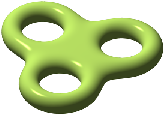
\includegraphics[scale=1.25]{main/Fig02-RiemannSurface}}
\vskip-15pt
\caption{A Riemann surface of genus 3.
\marginparhere{\redden{call in text?}}
}
\label{RiemannSurface}
\end{figure}


\begin{fact} (Hodge theory)
The sole topological invariant of a smooth projective curve $C$,
viewed as an analytic space, is its genus. As a manifold it is a
compact, oriented surface, and its genus is half the rank of its first
singular cohomology, $H^{1}(C; \CC)$, which is equal to its first 
de Rham 
cohomology.
Breaking up the de Rham cohomology of any smooth projective complex variety $X$ in terms of holomorphic and antiholomorphic differential
forms we get the \emph{Hodge decomposition}
$$
H^i(X,\CC) = H^i_{\mathrm{de\,Rham}}(X) = 
\tsty\bigoplus\limits_{j=0}^i H^j(\mwedge^{i-j} \Omega_X).
$$
For a smooth curve $C$, this says in  particular that
$$
H^1(C; \CC) = H^0(\omega_C)\oplus H^1(\sO_C) = H^0(\omega_C)\oplus (H^0(\omega_C))^\vee, 
$$
so $ h^0(\omega_C)$ is half the rank of the middle singular cohomology
group, justifying the name ``genus''. For details, 
see~\cite[p.\,116]{Griffiths-Harris1978}.
\end{fact}

A divisor $E$
of negative degree 
satisfies the equation
$H^0(E) = 0$,
so we get the form of the Riemann--Roch theorem
originally proved by 
\blue{Riemann:}
\index{Riemann, Georg}%

\begin{corollary}\label{nonspecial RR}
For any divisor $D$ of degree $d$ we have
$$
h^0(D) \geq d - g + 1,
$$
with equality if $d > 2g-2$.
\end{corollary}
%
It was 
\blue{Gustav Roch,}
\index{Roch!Gustav}%
a student of
Riemann's, 
who supplied the correction term $h^0(K_C - D)$ for divisors of lower degree.
The dimension $h^0(K_C-D) = h^1(D)$ was called the 
\blue{\emph{superabundance}}
\index{superabundance}%
of $D$: the ``expected'' number of sections was $d-g+1$, and $h^1(\cL)$ reflected how much larger the actual number was.

Corollary~\ref{nonspecial RR} and Proposition~\ref{very ample} together show that all high degree divisors come from hyperplane sections in 
suitable embeddings; and unlike the general vanishing theorems, they give a bound on the degree necessary for vanishing
of cohomology and for
global generation:

\begin{corollary}\label{degree 2g+1 embedding}
Let $D$ be a divisor of degree $d$ on a smooth, connected projective curve of genus $g$.
\begin{enumerate}
 \item If $d>2g-2$ then $H^1(\sO_C(D)) = 0$.
 \item If $d \geq 2g$ then $\sO_C(D)$ is generated by global sections; that is, the complete linear series $|D|$ is basepoint free; and $\sO_C(D)$ is very ample unless $D = K_{C}+E$ for some divisor $E$ of degree 2.
 \item If $d \geq 2g+1$ then $\sO_C(D)$ is very ample; that is, the associated morphism $\phi_D : C \to \PP^{d-g}$ is an embedding, and
$D$ is the preimage of the intersection of $C$ with a hyperplane in $ \PP^{d-g}$.
\end{enumerate}
\end{corollary}

\begin{proof}
If $d>2g-2$ then $K-D$ has negative degree, and thus 
$$h^1(D) = h^0(K-D) = 0. $$ 
The last two parts follow
from the Riemann--Roch theorem and Proposition~\ref{very ample}.
\end{proof}

Since the complement of a hyperplane in projective space is an affine space, we get an affine embedding result too:

\begin{corollary}
 If $C$ is any smooth projective curve and $\Gamma \subset C$ a nonempty finite subset then $C \setminus \Gamma$ is affine (that
 is, isomorphic to a closed subscheme of an affine space).
\marginpar{moved period past parens}     
\end{corollary}

\begin{proof}
Let $D$ be the divisor defined by $\Gamma$. By Corollary~\ref{degree 2g+1 embedding} a high multiple of $D$ is very ample,
and gives an embedding $\phi: C\to \PP^n$ such that the preimage of the intersection of $C$ with some hyperplane $H$
is a multiple of $D$. It follows that $C\setminus \Gamma$ is embedded in $\AA^n = \PP^n\setminus H$.
\end{proof}
 
We can  use Corollary~\ref{nonspecial RR} to determine the Hilbert polynomial of a projective curve. To do this, let $C \subset \PP^r$ be a smooth curve of degree $d$ and genus $g$, and consider the exact sequence of sheaves
$$
0 \to \cI_{C/\PP^r}(m) \to \cO_{\PP^r}(m) \to \cO_C(m) \to 0
$$
and the corresponding exact sequence
$$
 H^0(\cO_{\PP^r}(m)) \ruto{\rho_m} H^0(\cO_C(m)) \to H^1(\cI_{C/\PP^r}(m)) \to 0.
$$

The  $h_C$ of $C$  is defined in terms of the
\blue{\emph{Hilbert function}}
\index{Hilbert function}%
homogeneous coordinate ring $R_{C}$ of $C$ by
\marginpar{removed colon}
$$
h_C(m) = \dim_{\CC} (R_{C})_{m} = \rank \rho_m,
\marginparhere{removed parentheses around argument of rank}
$$
where $(R_{C})_{m}$ is the degree $m$ component of the homogeneous coordinate ring of $C$ in $\PP^n` `$.

By Theorem~\ref{Serre--Grothendieck vanishing} we have
$H^1(\cI_{C/\PP^r}(m)) = 0$ for large $m$.
\redden{Therefore}
\marginpar{to allow line break}
$h_{C}(m) = h^0(\cO_C(m))$ for large $m$, which, by 
\redden{Riemann--Roch}, equals $dm-g+1$, again for large $m$. 
Thus, the Hilbert polynomial of $C \subset \PP^r$ is $p_C(m) = dm-g+1$.  
More generally, we define what is called the \emph{arithmetic genus}:

\begin{definition}\label{genus Hilbert}\label{pa}\label{genus formula}
If $C\subset \PP^n$ is a 1-dimensional projective scheme with Hilbert polynomial
$p_C(m) = \chi(\sO_C(m))$, the \emph{arithmetic genus} of $p_a(C)$ is $1-\chi(\sO_{C}) = 1-p_C(0)$. If $C$ is reduced and irreducible, then
the \emph{geometric genus} $g(C)$ is the genus of the normalization of $C$.
\end{definition}

We see from the Riemann--Roch theorem that if $C$ is smooth and connected, then $p_a(C) = g(C) = h^0(\omega_C)$, the genus of $C$. We
will see that for reduced and irreducible curves $p_a(C) \geq g(C)$, with equality only when $C$ is smooth.
  For some examples with curves that are not
reduced and irreducible, see Exercise~\ref{pa example}.
  

The Riemann--Roch theorem and Serre duality have extensions to arbitrary coherent sheaves in place of invertible sheaves 
and to singular curves, which we will explain in Chapter~\ref{LinkageChapter}.

Divisors $D$ for which $h^0(K_C - D)>0$ are called \emph{special divisors}. The existence or nonexistence of divisors $D$ with given $h^{0}(D)$ and $h^{1}(D)$ often serves to distinguish one curve from another, and will be an important part of our study.

\subsection*{Residues, and a complex analytic argument for 
the Riemann--Roch theorem} 

The 
\marginpar{\vskip-35pt \hskip-14pt{\Large$\downarrow$} the hyphen in ``theorem'' is ugly, but I've been unable to fix it. Perhaps drop ``the'' and ``theorem'' around RR? It will lighten up the section title.\\[4pt]dropped ``as well'' after red text.}
Rie\-mann--Roch theorem is so central to the study of curves that it is worth understanding from another point
\redden{of view.}
We remarked at the beginning of Chapter~\ref{linear series} that a
smooth projective curve over $\CC$ is the same thing as a compact
Riemann surface. 
\redden{Here we will briefly adopt}
the complex analytic viewpoint, and give an explanation of 
\index{complex analytic viewpoint}%
\marginpar{\hskip-50pt $\leftarrow$ streamlined; also removed hyphen in ``complex analytic'' in
  section header to agree with this instance and Chapter 1}
a special case of Theorem~\ref{RR theorem}.

If $D = \sum a_ip_i$ is an effective divisor 
\marginpar{new paragraph}
on a compact Riemann surface $X$ then we write $L(D)$ 
for the vector space of meromorphic functions on $X$ with poles of order 
\marginpar{$\leq\,\to$ at most}
at most $a_i$ at $p_i$. 

\begin{theorem}
Let $X$ be a compact Riemann surface of genus $g$, and let $D$ be an effective divisor of degree $d$ on $X$. Suppose that $K-D$ is also effective for some canonical divisor $K$.
The dimension of  $L(D)$ is
$d-g+1+\dim_\CC L(K-D)$.
\end{theorem}
% avoid double skip
Because  meromorphic functions on a Riemann surface are rational functions on the corresponding
algebraic curve, and $L(D) = H^0(\sO_C(D))$, the assertion is equivalent to Theorem~\ref{RR theorem}.

\begin{proof}
% We will prove this using residues, under the additional assumption that  $D$ and $K-D$ are both effective (that is, $D$ is both effective and \emph{special} in the sense that there are nonzero functions
%both in $L(D)$ and in $L(K-D)$.)
%
Recall that the 
\blue{\emph{residue}} 
of a meromorphic 1-form $\phi$ at a
\index{residue}%
point $p$ on $X$ is defined by an integral: choose a disc $\Delta \subset X$ containing $p$ and in which $\phi$ is holomorphic except
\marginpar{replaced \{\string\rm\ res\} by \string\Res\ (defined with \string\operatorname\string) for the reasons explained in my email to the AMS}
for its pole at $p$. The residue $\Res_p(\phi)$ is $\sfrac{1}{2\pi i}$
times the integral of $\phi$ along the boundary of $\Delta$. If $z$ is
a local coordinate on $\Delta$ zero at $p$ and we write the
differential $\phi$ as
{\meshing
$$
\phi = \sum_{i=-n}^\infty \!a_iz^i \,dz
$$
then by Cauchy's formula, the residue of $\phi$ at $p$ is the coefficient $a_{-1}$. 
}

\begin{proposition}\label{residue sum}
 If $\phi$ is a meromorphic differential on a compact Riemann surface $X$, then the sum of the residues of $\phi$
 at all the poles of $\phi$ is $0$.
\marginpar{made 0 upright, ok?}
 \end{proposition}
 
\begin{proof}
Apply 
\blue{Stokes' theorem}
\index{Stokes' theorem}%
to the complement of the union of small discs around each of the poles of $\phi$.
\end{proof}

Let  $D = \sum a_ip_i$ be an effective divisor on $X$, and set $d = \sum a_i = \deg D$. Locally, a function with a pole of order at most $n$ at $p$ may be written in terms of a local coordinate $z$ at $p$ as $\sum_{i=-n}^\infty a_{i}z^{i} $;
the sum $\sum_{i=-n}^{-1} a_{i}z^{i}$ is called its \emph{polar part}.
By the maximum principle, a meromorphic function in $L(D)$ is determined, up to the addition of a constant, by its polar parts at the points~$p_i$. Thus we have $\dim L(D) \leq d+1$.
{\meshing\par}

When is a given collection $c_1,\dots,c_d \in \CC[z^{-1}]$ the polar parts of a global meromorphic function $f$ on $X$? A necessary condition
is that if $\phi \in L(K)$ is a holomorphic differential on $X$, then
$$
\sum \Res_{p_i}(f \cdot \phi) = 0.
$$
This gives $g$ linear relations on the $c_i$. However, if $\phi$ is a holomorphic differential vanishing at all the points $p_i$
then the corresponding relation is trivial. Thus the number of linearly independent relations on the polar parts of $f$ is actually $g - \dim L(K-D)$; and we arrive at an inequality
$$
\dim L(D) \leq d + 1 - g + \dim L(K-D).
$$

This is a priori only an inequality. But we can apply the same logic to an effective divisor $K-D$, and we see that
\begin{align*}
\dim L(K-D) &\leq \deg(K-D) + 1 - g + L(K - (K-D)) \\
& = 2g - 2 - d + 1 - g  + L(D) \\
&= g - d - 1 + L(D).
\end{align*}
Adding the two inequalities we have
\marginpar{\vskip-20pt added period}
$$
L(D) + L(K-D) \leq L(D) + L(K-D).
$$
Since the sum of the inequalities is an equality, we conclude that each inequality is also an equality; this is the Riemann--Roch formula
in our special case.
\end{proof}

\subsection*{Arithmetic genus and geometric genus}

Throughout this book, we will be primarily concerned with the geometry of smooth curves. Of course singular curves will arise\emdash for example, as images of smooth curves under morphisms that are not embeddings. At least when $C$ is a 1-dimensional variety (that is, a 
reduced irreducible 1-dimensional scheme) we can  regard $C$ as the image of a smooth curve in an optimal way:
\marginpar{replaced ``(Proposition~\ref{resolution of singularities})'' by colon}

\begin{proposition}\label{resolution of singularities}
If $C_0$ is a projective variety of dimension 1 then the \emph{normalization} $\phi: C \to C_0$ of $C_0$ is a birational
morphism from a smooth curve $C$. The curve $C$ is again projective, and the pair $(C, \phi)$ is
unique up to  isomorphism. In particular, every birational map of smooth curves is an isomorphism.
\end{proposition}
 
\begin{proof}
  We use the result that the normalization ($=$ integral closure) of a domain
finitely generated over a field is again finitely generated, and nonsingular in codimension 1 \cite[Theorem 4.14 and 11.5]{Eisenbud1995}. Thus,
starting with a projective embedding of $C$ we normalize the homogeneous coordinate ring of $C$. The resulting ring
may have generators in many degrees, but a suitable Veronese subring will be generated in a single degree, and thus
is the homogeneous coordinate ring of a smooth projective curve. 

Localization
\marginpar{reworded to avoid unpleasant hyphens}
commutes with normalization, and any map from a normal ring to a
domain factors uniquely through the normalization. 
\redden{Therefore}
the normalization is unique.
\end{proof}

A different, less canonical procedure for finding a smooth curve birational to a given curve
is explained in 
\marginpar{the xref here was undefined; I assume the last 3 exercises are relevant and coded accordingly. Please check}
\redden{Exercises \ref{Veronese of plane curve} to \ref{Mumford resolution argument}}.


Still assuming that $C_0$ is reduced and irreducible, we can relate
\marginpar{it's it obvious what these terms mean?}
\index{arithmetic genus}%
\index{geometric genus}%
\index{genus!arithmetic versus geometric}%
the
\redden{arithmetic and geometric genera}
of $C_0$ using the map of sheaves
$$
\cO_{C_0} \to \nu_*\cO_C.
$$
Since the normalization map of rings  is injective and finite, this map is injective. The cokernel $\sF$ is a coherent sheaf supported on the singular points of $C_0$, and is thus finite over $\CC$. 
The definition implies that there is a short exact sequence
$$
0 \to \cO_{C_0} \to \nu_*\cO_C \to \cF \to 0.
$$

\begin{proposition}\label{pa and delta}
Suppose that $C_{0}$ is a reduced, irreducible curve and let  $\nu: C\to C_{0}$ be its normalization.
Let $\sF = \nu_{*}\sO_{C}/\sO_{C_{0}}$. If we set 
$\delta(C_{0}) := h^{0}(\sF)$, 
\redden{then}
 $$
p_a(C_0) - g(C) =  \delta(C_{0})
$$ 
\end{proposition}

\begin{proof}
 Since the normalization map $\nu: C \to C_0$ is finite,  the direct images $R^i\nu_*\cO_C$ vanish for $i > 0$, 
so the Leray spectral sequence 
\redden{(see \ref{Leray} just below)}
computes $\chi(\nu_*\cO_C) = \chi(\cO_C)$. Thus
$$
p_a(C_0) - g(C) =  \chi(\cO_{C}) -   \chi(\cO_{C_0}) = \chi(\cF) = h^0(\cF) 
$$ 
since the support of $\cF$ is finite.
\end{proof}

The operation of normalization localizes, so we can understand $\sF$ by looking at it locally.
Writing $R$ for the affine ring of some affine subset $U\subset C_{0}$ we see that $\sO_{C}|_{U}$
is the integral closure $\ovR$ of $R$, so $\sF|_{U}$ is $\ovR/R$. Thus
the annihilator of $\sF|_{U}$, called the \emph{conductor}
$\ff_{\ovR/R}$,
\marginpar{added comma before red phrase}
\redden{is an ideal of both $\ovR$ and $R$,}
and correspondingly $\nu^{-1}(\ff_{C/C_{0}})$ 
is also an ideal sheaf in $\sO_{C}$.

Informally, we may say that $\delta(C_{0})$ is the number of linear
conditions a locally defined function $f$ on $C$ has to satisfy to be
the pullback of a function from $C_0$. The length of the stalk of
$\cF$ at a particular singular point $p \in C_0$ is called the
\index{delta invariant|$\delta$-invariant}
\emph{$\delta$-invariant} $\delta_p$ of the singularity. Thus 
\marginpar{semicolon $\to$ colon; added punctuation in display}
$$
p_a(C_0) - g(C) = \sum_{p @\in@ (C_0)_{\mathrm{sing}}\!\!} \delta_p.
$$ 

\begin{fact}~\label{Leray}
 In general, the 
\blue{Leray spectral sequence}
\index{Leray spectral sequence}%
addresses the situation of  a morphism $f:X\to Y$ of varieties or schemes, 
 and a coherent sheaf $\sG$  on the source $X$; it says in this circumstance that there is a spectral sequence
  $$
  \HH^p(R^qf_*(\sG)) \Longrightarrow \HH^{p+q}(\sG).
  $$
(This is a special case of the spectral sequence for the derived functors of a composite functor ($H^0$ composed with $f_*$);
see~\cite[II.4.17.1]{Godement} or \cite[Section III.7]{Gelfand-Manin} for proofs.)
\end{fact}

In the simplest cases the $\delta$ invariant is easy to compute:


\begin{enumerate}

\item A 
\index{node}%
\blue{\emph{node}}
of a curve $C_0$ is a point $p$ such that
\marginpar{removed ``(nodes)''}
  an analytic neighborhood of $p$ in $C_0$ consists of two smooth arcs
  intersecting transversely at $p$ 
\redden{(See Figure \ref{simplesing}, left.)}
Equivalently, the completion of
  the local ring $\cO_{C_0,p}$ is isomorphic to $k\[x,y\]/(xy)$. If $p
  \in C_0$ is a node, its preimage in the normalization $C$ of $C_0$
  consists of two points $r,s\in C$. The condition for a function $f$
  on $C$ to descend to $C_0$\emdash that is, to be the pullback of a function
on $C_0$\emdash is  that $f(r)=f(s)$; this is one 
linear condition, so $\delta_p = 1$.

\item  
\redden{A}
\index{cusp!ordinary}%
\blue{\emph{cusp}} 
\marginpar{I'm reacting here to the ``(cusps)'' in parens in the versus the term actually defined.}
\redden{(strictly speaking, an \emph{ordinary cusp})}
of a curve $C_0$ is a point $p$
  such that an analytic neighborhood of $p$ in $C_0$ is given by the
  equation $y^2=x^3` `$. 
\redden{(See Figure \ref{simplesing}, second from left.)}
If $p \in C_0$ is an ordinary cusp then its
  preimage in the normalization $C$ of $C_0$ will consist of one point
  $r\in C$. The condition for a function $f$ on $C$  is that the
  derivative $f'(r)=0$; again, this is one linear condition, so
  $\delta_p = 1$. 
\marginpar{moved \string\end\{enumerate\} so the break appears before ``We will''}
\end{enumerate}

We will give more examples at the end of
Chapter~\ref{PlaneCurvesChapter}.



\begin{figure}   % appears as 2.4
\centerline{%
  \includegraphics[height=2in]{"main/Fig02-sing-node"}\hfil\quad
  \includegraphics[height=2in]{"main/Fig02-sing-cusp"}\hfil\quad
  \includegraphics[height=2in]{"main/Fig02-sing-tacnode"}\hfil\quad
  \includegraphics[height=2in]{"main/Fig02-sing-triple"}}
\caption{Simple planar curve singularities.
\index{tacnode}%
\index{triple point}%
\index{planar curve singularities}%
\index{singularity!of planar curve}%
\label{simplesing}
}
\end{figure}


\section{The canonical morphism}

We now return to the world of smooth curves.
\index{canonical morphism}\index{morphism!canonical}%

 The canonical sheaf on $\PP^1$ has negative degree, so $|K_{\PP^1}| = \emptyset$. If $C$ is a curve
 of genus $1$ then the canonical sheaf     has a nonzero global section, and since the sheaf has degree $2g-2=0$ this is nowhere vanishing, whence
 $\omega_C = \sO_C$, and $K_C = 0$. Thus in studying the canonical series we restrict our attention to curves $C$ of genus $g\geq 2$. 
 
 \begin{theorem}\label{canonical series is very ample} Let $C$ be a smooth curve of genus $\geq 2$.
\begin{enumerate}
 \item $|K_C|$ is basepoint free.
 \item $|K_C|$ is very ample if and only if $C$ admits no map of degree 2 to $\PP^1` `$.
\end{enumerate}
\end{theorem}

A curve of genus $\geq 2$
is said to be \emph{hyperelliptic} if there exists a 
\blue{morphism}
$f: C \to \PP^1$ 
\begingroup\def\marginpar#1{}%
\blue{of degree 2.}
\endgroup
\index{hyperelliptic}%
\index{morphism!of degree 2}%
It is easy to describe this in terms of linear series:

\begin{lemma}\label{deg 2 morphism}
Let $C$ be a smooth, projective curve of genus $g\geq 2$. If $C$ has an invertible sheaf $\cL$ of degree $\leq 2$ with two independent sections, then $\cL$ has degree~$2$ and
$|\cL|$ defines a morphism of degree $2$ to $\PP^{1}$, so $C$ is
hyperelliptic. In particular, if $g(C) = 2$ then the canonical series
\marginpar{hyphenated 2-to-1 (and uprighted digits in statements) to agree with the math occurrences}
$|K_{C}|$ defines a $2$-to-$1$ morphism to $\PP^{1}$, so $C$ is
hyperelliptic.
\end{lemma}

\begin{proof}
Since $C \not\cong \PP^1` `$,  Theorem~\ref{characterization of P1} shows that $C$ cannot have a 1-dimensional linear series
of degree $< 2$. Thus $\sL$ has degree exactly 2, and no 
\marginpar{\redden{You defined ``base point'' in chapter 1; this must be the same thing, but here you're writing it as one word. Either is fine, but we should be consistent.  I lean toward no space, since ``base point free'', ``base-point free'' or ``base-point-free'' are all awkward. But it's up to you.}}
\redden{basepoints,}
so it defines a morphism of degree 2 to $\PP^1$ as claimed.
\end{proof}

\begin{proof}[Proof of Theorem~\ref{canonical series is very ample}]
A point $p$ is a basepoint of $|K_C|$ if and only if 
\marginpar{displayed to allow line break}/that
$$h^0(K_C-p) = h^0(K_C) = g.$$ 
By the Riemann--Roch theorem,
this is eqivalent to $h^0(p) =2$, which would imply that $C\cong \PP^1$ by Theorem~\ref{characterization of P1}. Thus $K_C$
has no basepoints.

By Proposition~\ref{very ample} we 
\redden{must}
show that for any 
\redden{two}
points $p, q \in C$ we have
\unskip\marginpar{for better layout}
$$
h^0(K_C(-p-q)) = h^0(K_C)-2 = g-2.
$$
Applying the Riemann--Roch theorem we see 
\marginpar{added ``that'' to allow line break}
that this fails if and only if $h^0(\cO_C(p+q)) \geq 2$ for some $p,q
\in C$. By Lemma~\ref{deg 2 morphism}, this implies that $C$ is
hyperelliptic. Conversely, if $C$ is hyperelliptic then for some
divisor $D = p+q$ we have $h^0(D) = 2$, whence $h^0(K-p-q) = h^0(K)
-1$ by 
the Riemann--Roch formula.
\emergencystretch5.5pt
\end{proof}

The image of the canonical morphism of a nonhyperelliptic curve of
genus $g>2$ is called a 
\blue{\emph{canonical curve},}
\index{canonical curve}%
and (for a nonhyperelliptic curve) we  
speak of the image as being \emph{canonically embedded}.


\subsection*{Geometric Riemann--Roch}

There is a useful way of expressing the Riemann--Roch formula in terms
of the geometry of the canonical map. Suppose $C \subset \PP^r$ is a
smooth curve and $D$ an effective divisor on $C$, thought of as a
subscheme of $C$. We define the 
\blue{\emph{span}}
\index{span!of effective divisor}%
$\ovD$ of $D$ to be the
\marginpar{the index entry is ``span of effective divisor; this covers $\overline{\phi(D)}$ as well, right?}
intersection of the hyperplanes $H \subset \PP^r$ containing $D$. More
generally, if $\phi : C \to \PP^r$ is a map and $D$ an effective
divisor on $C$, we define the span $\overline{\phi(D)} \subset \PP^r$
to be the intersection 
$$
\overline{\phi(D)} := \bigcap_{ 
\substack{H \subset \PP^r \text{ a hyperplane} \\D \subset
  \phi^{-1}(H)}}
H.
\marginparhere{stacked conditions to avoid superwide subscript, ok?}
$$

Now suppose $C$ is a smooth curve of genus $g\geq 2$ and $\phi_K: C\to \PP^{g-1}$ is the canonical morphism.
If  $D$ is an effective divisor on $C$ of degree $d$, then since the hyperplanes in $\PP^{g-1}$ containing $\phi_K(D)$ correspond (up to scalars) to sections of $K_C$ vanishing on $D$, we see that
$$
h^0(K_C-D) = \codim \overline{ \phi_K(D)} \subset \PP^{g-1}= g - 1 - \dim \overline{ \phi_K(D)}.
$$
\index{geometric!Riemann--Roch theorem}%
\index{Riemann--Roch theorem!geometric}%
Applying the Riemann--Roch theorem we obtain  the \emph{geometric Riemann--Roch theorem}:

\begin{corollary}\label{geometric RR}
If $D$ is a divisor on a smooth curve $C$ of genus $\geq 2$ then
$$
r(D) = d - 1 - \dim \overline{ \phi_K(D)}.
\vspace*{-3pt}
$$
\end{corollary}
%
In particular, if $D = \sum_{i=1}^dp_i$ is a sum of distinct points, then
 the dimension of the linear series $|D|$  is equal to the number of linear relations among the images of the $p_i$ on the canonical 
 image of $C$. 
 Thus, for example, a divisor given as the sum $D = p+q+r$ of three
 points will move in a pencil if and only if the three points are
\marginpar{\hskip-100pt $\leftarrow$ colinear $\to$ collinear (there were about equal numbers of each, I uniformized toward the old-fashioned spelling, ok?\\[3pt] streamlined passage in red; original had $\mathrm{p}_{\mathrm{a}})$, but that  seems to have been a coding error}
 collinear on the canonical model. 

In general, 
the condition on forms of degree $d$ to vanish at 
\redden{a given point $p$ in $\PP^r$ is expressed}
by one homogeneous linear
 linear equation on the coefficients of the form, obtained by evaluating the variables at 
 the coordinates of $p$, so vanishing on a set $\Gamma$ of $\gamma$ points is given by
 $\gamma$ linear equations and the same is true when $\Gamma$ is a finite subscheme
 of length $\gamma$, as one sees from the exact sequence
 $$
 0\to H^0(\sI_\Gamma(d) \to H^0(\sO_{\PP^r}(d)) \ruto{ev} H^0(\sO_{\Gamma}(d)) \to 0,
 $$
 bearing in mind that 
 $$
 H^0(\sO_{\Gamma}(d)) \cong H^0(\sO_{\Gamma}) \cong \CC^\gamma.
 $$
However, the linear equations may be linearly dependent; that is, the map marked $ev$
above may have rank $<\gamma$. We will say that the points of $\Gamma$
\emph{fail to impose independent conditions on hypersurfaces of degree $d$}
by the amount equal to $\gamma - \rank(ev)$. 

With this terminology, the geometric Riemann--Roch theorem says that 
the dimension of the complete linear series $|D|$ on a smooth curve $C$
is the amount by which the points of $D$ fail to impose independent conditions
on canonical divisors, and the geometric version simply translates this into 
 hyperplanes in the canonical embedding of $C$. 
\index{Cayley--Bacharach--Macaulay theorem}%
The Cayley--Bacharach--Macaulay
theorem~\ref{CBM} and the result of 
\marginpar{\redden{missing xref `pluricanonical'}}
Exercise~\ref{pluricanonical} are other useful
special cases.

\begin{remark}
For a singular curve $C_0$ to have a canonical morphism it is necessary first of all that its canonical sheaf
 $\omega_{C_0}$ be invertible; when this is the case, we say that $C_0$ is (locally) Gorenstein, and then
\index{locally Gorenstein}%
\index{Gorenstein!locally}%
the theory above can be applied. See for example \cite{graphcurves} and \cite{ribbons} for examples. 
\end{remark}

\subsection*{Linear series on a hyperelliptic curve}
We can describe the canonical map of a hyperelliptic curve\emdash and indeed all its special linear series\emdash quite precisely:

\begin{corollary}\label{canonical on hyperelliptic}
Let $C$ be a smooth hyperelliptic curve of genus $g\geq 2$. The curve $C$ admits a unique degree 2 morphism $\pi: C\to \PP^1` `$,
and the canonical map $\phi_K: C\to \PP^{g-1}$ is the composition of $\pi$ with the Veronese map of degree $g-1$ from
\index{Veronese map}%
$\PP^1$ to the rational normal curve of degree $g-1$; in particular, every canonical divisor is a sum of $g-1$ fibers of $\pi$ and vice versa.
\end{corollary}

\begin{proof}
If $D$ is a general fiber of a degree 2 map $\pi:C\to \PP^1$ so that $D= p+q$ and $r(D) = 1$, then by the Riemann--Roch theorem or its geometric version, $D$ imposes only one condition on sections of $K_C$; that is, $\phi_K(p) = \phi_K(q)$. Consequently the degree of the canonical morphism $\phi_K$ is at least 2, and the image is thus a nondegenerate curve in $\PP^{g-1}$ of degree $\leq (2g-2)/2 = g-1$. By Theorem~\ref{characterization of P1}, the image of $\phi_K$ is the rational normal curve of degree $g-1$ and every fiber of $\phi_K$ is a divisor linearly equivalent to $D$. It follows that $\pi$ is determined by $K$, so it is unique. Since every canonical divisor is the pullback of a hyperplane section of the rational normal curve,
every canonical divisor is a sum of $g-1$ fibers of $\pi$.
\end{proof}

We can use these ideas to analyze all special divisors.
\index{special divisor}%
\index{divisor!special}%

\begin{corollary}\label{special on hyperelliptic} Let $C$ be a smooth 
\blue{hyperelliptic curve}
\index{hyperelliptic curve}%
with map $\pi: C\to \PP^1$ of degree 2.
Every special divisor $D$ of degree $d$ on 
\marginpar{a hyperelliptic curve $\to C$}
$C$ is a sum of $s$ fibers of $\pi$ and $d-2s$ points
$p_1,\dots,p_{d-2s}$ with distinct images under the canonical map; and
in this case we have $r(D) = s$ and the points $p_i$ are base points
of the linear series $|D|$.
\end{corollary}

\redden{Thus}
\emph{no divisor on a hyperelliptic curve is both special and very ample}.
\marginpar{streamlined}

\begin{proof}
Suppose that $D$ contains the sum $E$ of $s$ fibers of $\pi$ and no more; and write $D = E+D'$, with $\deg D' = d-2s$.
 
If $\phi_K:C \to \PP^{g-1}$ is the canonical map, then $\phi_K(D')$ consists of $d-2s$ distinct points, while $\phi_K(E)$ consists of
$s$ points. By Corollary~\ref{independence of points on a RNC} the span of $\phi_K(D)$ has dimension $\min\{g-1, d-s-1\}$, so 
$r(D) = d-1-\min\{g-1, d-s-1\} = \max \{s,d-g\}$. Since $D$ is a special divisor, $r(D) > d-g$, so $r(D) = s$. 
Since $r(E) =s$, we see that $E$ is basepoint free, so $D'$ is the base locus of $D$.
\end{proof}

\section{Clifford's theorem}\label{Clifford Section}

While the Riemann--Roch theorem gives a lower bound for the dimension of a linear series, $r(\sL) := h^0(\sL)-1 \geq \deg \sL -g$, Clifford's theorem
\index{Clifford's theorem}%
gives an upper bound. If $\deg \sL>2g-2$, then the Riemann--Roch
inequality becomes an equality, so it is enough to treat the case
$\deg \sL \leq 2g-2$. The bound is actually a corollary of the 
Riemann--Roch theorem.

\begin{corollary}\label{Clifford bound}
 Let $C$ be a curve of genus $g$ and $\cL$ a line bundle of degree $d \leq 2g-2$. Then
$$
r(\cL) \leq \frac{d}{2}.
$$
\end{corollary}

\begin{proof}
If $\cL$ is nonspecial then, since $g\geq d/2 + 1$, we have $r(\cL) = d-g+1\leq d/2$.
Otherwise we have
$$
r(K_C\otimes \cL^{-1}) = r(\cL) +g - d - 1
$$
by the Riemann--Roch theorem,
and so by Proposition~\ref{sum of linear series}
$$
g = r(K_C)+1  \geq r(\cL) + r(K_C\otimes \cL^{-1}) +1  = 2r(\cL) +g - d;
$$
hence $r(\cL) \leq d/2$.
\end{proof}

The usual statement of Clifford's theorem includes a description of when equality can occur:

\begin{theorem}\label{Clifford}\label{Clifford equality}
Let $C$ be a curve of genus $g$ and $\cL$ a line bundle of degree $d \leq 2g-2$. If
$$
r(\cL) = \frac{d}{2},
$$
the largest possible value, then either
\begin{enumerate}
\item $d=0$ and $\cL = \cO_C@$;
\item $d = 2g-2$ and $\cL = K_C@$; or
\item $C$ is hyperelliptic, and $|\cL|$ is a multiple of the $g^1_2$ on $C$.
\end{enumerate}
\end{theorem}

From Corollary~\ref{canonical on hyperelliptic} and Corollary~\ref{geometric RR} we see that the equality does indeed hold
in each of the cases enumerated. See
Corollary~\ref{equality in Clifford from Martens} for the converse and \cite[IV.5.4]{Hartshorne1977}
for a different proof.

 \section{Curves on surfaces}\label{surface basics}
 
 We will often analyze curves  on a smooth surface. Compared to the theory of linear series on curves, there is a new element: the intersection pairing. We refer to~\cite[Chapter V]{Hartshorne1977}
\index{intersection pairing}%
 and~\cite[Chapter I]{Beauville} for 
\marginpar{``proof'' ok? Or would ``proofs'' be better?}
\redden{proof} 
of the unproven statements in this section.
 We suppose for this section that $S$ is a smooth projective surface,
 and write $\Pic(S)$ for the group of invertible sheaves on $S$.

\subsection*{The intersection pairing}

When two codimension-1 subschemes $D,E$ on $S$ 
\marginpar{upgraded to a subsection (instead of subsub; see also note at top of page 50}
meet transversely we define $D\cdot E$ to be the number of points in which they meet.  
It is less obvious how one might define an intersection number $D\cdot E$ in more general cases,
including the case $D=E$. However 
a codimension-1 subvariety of $S$ has a 
\index{fundamental class}%
fundamental class in $H^{2}(X,\ZZ)$, and the product just defined
agrees with the cup product pairing
\index{cup product pairing}%
$$
H^{2}(S,\ZZ) \times H^{2}(S,\ZZ) \to H^4(S,\ZZ)\cong \ZZ,
$$
showing that it is possible. For example, the self-intersection $D\cdot D$ can be realized geometrically
 by choosing a  vector field $\sigma$ on $D$ and using it to push a copy $D'$ of $D$ infinitesimally away from $D$; then
 one can count the points where $\sigma$ becomes tangent to $D$. Here one must take orientations into account,
 and the result is that $D\cdot D$ may be negative. In the previous case (and when $\sigma$ is complex analytic)
 the multiplicities are all positive because a complex subvariety is canonically oriented using the orientation of $\CC$
 itself.

\begin{figure}   % appears as 2.5
\inprogress
\centerline {\includegraphics[height=1.75in]{"main/Fig02-strip"}}
\captionPlus{Fig02-strip}{The result, $D'$, of moving $D$ infinitesimally along a normal vector field meets $D$ twice.
\marginparhere{\hsize=2.5in\redden{call in text?} Also, this needs redrawing; the arrows are supposed to be perpendicular to the curve, but in perspective they may not look so, since the the supporting surface is not planar, right?}
}
\end{figure}

This pairing can be realized algebraically as follows:

First, if $D$ and $E$ have no common
\index{intersection multiplicity}%
components, then the \emph{intersection multiplicity} 
$m_S(D,E,p)$ at $p\in S$
is defined as the vector space dimension of the local ring $\sO_{S,p}/(\sI_{D,p}+\sI_{E,p})$, and 
$$
D\cdot E = \sum_p m_S(D,E,p).
$$

Quite generally, 
the intersection product can be computed using the (algebraic) Euler
characteristic. 
\marginpar{dropped ``and'' and started new sentence}
\redden{This}
works even for 
\blue{Cartier divisors}
on a singular surface: Setting $\sL := \sO_S(D)$ and
\index{Euler characteristic}%
\index{Cartier divisor}%
$\sM := \sO_S(E)$ to simplify the notation, we have 
$$
D\cdot E = \chi(\sO_S)-\chi(\sL^{-1}) -\chi(\sM^{-1}) +\chi(\sL^{-1}\otimes \sM^{-1}) 
.
$$

\begin{theorem} The pairing $(D,E) \mapsto (D\cdot E)$ is the unique bilinear map
$\Pic(S) \times \Pic(S) \to \ZZ$ extending the case of intersections of two curves meeting transversely at smooth points of $S$. 
\end{theorem}

An important special case is that of the self-intersection $D\cdot D = D^2` `$. The general formula reduces immediately to the case of an effective divisor, and in that case it resembles the $C^{\infty}$ construction above:

\begin{corollary}\label{self-intersection number}
If $D$ is a codimension $1$ subscheme of $S$, then the self-intersection $D\cdot D$ is the degree of the normal bundle
$\sN_{D/S} := \sO_{D}(D)$.
\end{corollary}

\begin{proof}
Substituting $\sO_{S}(-D)$ for both $\sL^{-1}$ and $\sM^{-1}$ we
\redden{have the}
\marginpar{streamlined and undisplayed sequences for better layout}
%compute from the short 
exact sequences
\begingroup
\thickmuskip = 4.5mu plus 1mu 
$ 0\to \sO_{S}(-D)\to \sO_{S}\to \sO_{D}\to 0@$ and 
$@0\to \sO_{S}(-2D)\to \sO_{S}(-D)\to \sO_{D}(-D)\to 0$;
the Riemann--Roch theorem 
\endgroup
\redden{then gives}
\begin{align*}
\chi(\sO_{S}) -\chi(\sO_{S}(-D)) &= \chi(\sO_{D}) = -p_{a}(D) +1,\\
\chi(\sO_{S}(-D)) -\chi(\sO_{S}(-2D)) &= \chi(\sO_{D}(-D)) = -\deg \sO_{D}(D) - p_{a}(D) +1.
\end{align*}
Subtracting the second of these equations from the first we see that
$D\cdot D = \deg \sO_{D}(D)$.
\end{proof}

Using the intersection pairing we can turn the adjunction formula of Proposition~\ref{adjunction} into a numerical formula:

\begin{theorem}[adjunction formula]\label{adjunction formula} 
If $C$ is a Cartier divisor on a smooth surface $S$ then
\index{adjunction formula}%
$$
p_a(C) = \frac{(K_X+C)\cdot C}{2} +1.
 $$
\end{theorem}

\subsection*{The Riemann--Roch theorem for smooth surfaces}
Often we wish to compute the dimension of the space of sections of an invertible sheaf, but
\marginpar{\redden{The section ``Curves on surfaces'' had three subsections: a long one on curves on quadrics, and two shorter ones.  As they seemed independent, I've placed the shorter ones first, and made the one on quadrics into a section (2G) instead of a subsection.}}
as with the case of curves, the Euler characteristic is more accessible:

\begin{theorem}[Riemann--Roch for surfaces] Let $\sL$ be an invertible sheaf on a smooth surface $S$.
\index{Riemann--Roch theorem!for surfaces}%
\index{Euler characteristic}%
The Euler characteristic $\chi(D) := h^0(\sL)-h^1(\sL)+h^2(\sL)$, where $\sL = \sO_S(D)$, is given by
$$
\chi(D) = \chi(\sO_S) + \frac{(D-K_S)\cdot D}{2}+1
.
\marginparhere{added punctuation in these and some other displays}
$$
\end{theorem}

\subsection*{Blowups of smooth surfaces}

It is useful to know what happens under mappings of surfaces, particularly the case of the mapping
\index{blowup!of smooth surface}
corresponding to blowing up a point.

\begin{theorem}\label{divisor classes on blowup}
If $\pi: X \to Y$ is a birational map of smooth surfaces, then the pullback map on divisors
preserves the intersection pairing. If $X$ is the blowup of~$Y$ at a point $p$ with exceptional
divisor $E = \pi^{-1}(p)$, then:

\begin{enumerate}
 \item $\Pic X =\pi^*(\Pic Y) \oplus \ZZ E$.
\item The canonical class on $X$ is given by $K_X = \pi^*(K_Y)+E$.
 \item The intersection pairing on $\Pic X$ is given by:
 
\begin{itemize}
\item $\pi^*(D)\cdot\pi^*(D') = D\cdot D'$ for all $D,D'\in \Pic Y$.
\item $\pi^*(D)\cdot E = 0$ for all $D\in \Pic Y$.
 \item $E\cdot E = -1$.
 \item $K_X\cdot E = -1$.
 \item If $C$ is a curve that has an $m$-fold point at $p$ then
   $\pi^{-1}(C)$ contains $E$ with multiplicity $m$, so that the 
\index{proper transform}
proper transform
 $\tilde C$\emdash that is, the closure in $X$ of the preimage of $C \setminus \{p\}$\emdash has class
 $$
 \tilde C \sim \pi^*C - mE.
 $$
 \end{itemize}
\end{enumerate}
\end{theorem}

Using these facts, we can compare the adjunction formula applied to a curve $C$ on a smooth surface $S$ to the formula applied to the proper transform $\tilde C \subset \tilde S$: we have
$$
\tilde C \cdot \tilde C = C \cdot C - m^2 \quad \text{and} \quad \tilde C \cdot K_{\tilde S} = C \cdot K_S + m.
$$
Combining these, we arrive at the formula
$$
p_a(\tilde C) = p_a(C) - \mbinom{m}{2},
$$
and thus the $\delta$-invariant of $p \in C$ is $\tbinom{m}{2}$ plus the sum of the $\delta$-invariants of all the 
points of $\tilde C$ in the preimage of $p$. One can resolve the curve singularity by repeatedly blowing up in this way and thus compute the $\delta$-invariant
of any singularity as a sum of binomial coefficients.

In the special case where $\tilde C$ is smooth\emdash for example, if
the point $p \in C$ is an \emph{ordinary $m$-fold point}, consisting
\marginpar{\redden{what should ``ordinary $m$-fold point'' be indexed under}}%
\index{ordinary $m$-fold point}%
of $m$ smooth branches with distinct tangent lines\emdash we conclude
that the $\delta$-invariant of the point $p$ is $\tbinom{m}{2}$. 


Blowups occur frequently in the theory of surfaces, and are
\index{Castelnuovo's theorem}%
characterized by \emph{Castelnuovo's theorem} 
\cite[Theorem V.5.7]{Hartshorne1977}. 

\begin{theorem}
If $E\subset X$ is a curve on a smooth projective surface $X$ and
\index{blow-down}%
 that $E^2 = E\cdot K_X = -1$ then $E$ can be ``blown down'' in the sense that
 $X$ is the blowup of a smooth surface $Y$ at a point $p\in Y$, and $E$ is the exceptional divisor.
\end{theorem}




\section{Quadrics in $\PP^3$ and the curves they contain}
\label{Div of quadric}
 
 We will frequently be interested in curves on a quadric surface in $\PP^3` `$, and we can describe these
curves and their intersections very concretely.

\subsection*{The classification of quadrics} The form defining a quadric $Q\subset \PP^{3}$ can be written in suitable
\index{classification of quadrics}\index{quadric!classification of --s}%
coordinates $x_{i}$ as 
$$q = \sum_{i=0}^{3} x_{i}^{2},$$ 
where $r\leq 4$ is the \emph{rank} of $Q$. (The corresponding
statement is also true in $\PP^{r}$, with $m\leq r+1$.) Equivalently, this is the rank of the symmetric matrix $M$
representing the bilinear form $\frac12(q(x+y)-q(x)-q(y))$.

\begin{enumerate}
\item A quadric of rank 1 is a double plane.
\index{double plane}%
\marginpar{changed to \{enumerate\} for ease of reference to the result in (d)}
\item A quadric of rank 2 is the union of two distinct planes. 
\item A quadric $Q$ of rank 3 is a cone over a smooth plane conic. The cone point is called the vertex. Every line
\index{vertex}%
on such a quadric passes through the vertex. The 
\blue{Picard group}
\index{Picard group}
of $Q$ is $\ZZ$
\cite[Exercise II.6.5]{Hartshorne1977}.
\marginpar{removed parens around cite}

\item A quadric $Q$ of rank 4 is smooth and is isomorphic to
  $\PP^{1}\times \PP^{1} \subset \PP^{3}$, embedded by the Segre
  embedding. Every line on such a quadric has the form $\PP^{1}\times
  \{p\}$ or $\{p\} \times \PP^{1}$; the two families of such lines are
  called 
\blue{\emph{rulings}.}
\index{ruling}%
\index{Segre embedding}%
\label{smooth quadric}
The Picard group of $Q$ is $\ZZ\times \ZZ$, generated by the lines of the rulings.
\cite[Example II.6.1]{Hartshorne1977}.
\marginpar{removed unmatched right parens}

\item Quadrics in $\PP^{r}$: Inside the space $\PP(\sO_{\PP^{r}}(2)) = \PP^{\binom{r+2}{2}-1}$ the space
of singular quadrics is a hypersurface of degree $r+1$, called the \emph{discriminant}, which is defined by the determinant of a generic symmetric
\index{discriminant}%
$(r+1)\times (r+1)$ matrix $M$. More generally, the rank $k$ locus is defined by the $(k+1)\times (k+1)$
minors of $M$.
\end{enumerate}

%\subsection*{Curves on quadrics}

\redden{It follows that}
\marginpar{\redden{the \{itemize\} here wasn't a coherent list. The first item became this paragraph and the next two became examples, because in an exercise, you referred to one of them as Example~(section number).}}
an irreducible nondegenerate  curve cannot be contained in a quadric of rank 1 or 2.

\subsection*{Some classes of curves on quadrics}

\begin{example}
Let $C$ be a reduced curve on a quadric $Q$ of rank 3 in $\PP^{3}$. 
If $C$ has even degree $2m$ then $C$ is a complete intersection
of the quadric with a hypersurface of degree $m$. Therefore if the curve is smooth it cannot contain the vertex of the quadric. The genus of $C$ is $(m-1)^{2}$.

If $C$ has odd degree $2m+1$, then the union of $C$ with a line on the quadric has even degree,
so if $L_{1}, L_{2}$ are lines on the quadric, then 
$$
C\cup L_{1} = Q\cap F_{1} \quad\hbox{and}\quad C\cup L_{2} = Q\cap F_{2}
$$
are complete intersections of $Q$ with forms of degree $m+1$, and the homogeneous ideal of $C$ is generated by the equations
of $Q,F_{1}$ and $F_{2}$. The genus of $C$ is $m(m-1)$. The curve $C$ contains the vertex, and is a 
\index{Weil divisor}%
\index{Cartier divisor}%
Weil divisor, not a Cartier divisor. These things follow from the description of the desingularization
of $Q$ in Corollary~\ref{singular scrolls}.
\end{example}

\begin{example}
\label{curves on quadrics}
If $C$ is a reduced curve on a quadric $Q$ of rank 4, then in terms of the isomorphism
$Q \cong \PP^{1}\times \PP^{1}$ we can express the divisor class of $C$ as $(a,b)\in \Pic(Q) = \ZZ\oplus \ZZ$.
The intersection form on $Q$ is determined by the fact that the lines of a ruling are all linearly equivalent,
so that $(1,0)^{2} = (0,1)^2=0$ and $(1,0)\cdot (0,1) = 1$; thus $(a,b)\cdot (d,e) = ae+bd$. The hyperplane section
has class $(1,1)$, and the canonical class is $(K_{\PP^{3}}+Q)\mid_{Q} = (-2,-2)$ by the adjunction formula. 

Thus
if $C$ has class $(a,b)$ then the degree of $C$ is $a+b$, while the genus of $C$ is $(a-1)(b-1)$. Note that 
if  $a =b$, the curve is a complete intersection, and if $b = a+1$ then the curve is residual to
a line in a complete intersection of the quadric with a surface of degree $b$. In these cases we get the same genus and degree as we would for a curve
on a rank 3 quadric.


The cohomology of $\sO_{Q}(a,b)$ is determined by the K\"unneth formula
\index{K\"unneth formula}%
\index{Leray spectral sequence}%
(or the Leray spectral sequence) as
$$
H^{i}(\sO_{Q}(a,b)) = \tsty\bigoplus\limits_{i = s+t}H^{s}
(\sO_{\PP^{1}}(a))\otimes H^{t}(\sO_{\PP^{1}}(b)).
$$
The degrees of the generators of the homogeneous ideal of $C$ can be determined from the exact sequence
$$
0\to \sI_{Q/\PP^{3}} \to \sI_{C/\PP^{3}} \to \sI_{C/Q} \to 0.
$$
Since $ \sI_{C/Q} (m) = (m-a,m-b)$ we see that, supposing $0<a\leq b$ and $1<b$
there are no generators other than the equation $q$ of $Q$ having degree $<b$, and there are 
$b-a+1$ generators of degree exactly $b$; with $q$ these are the minimal generators of the homogeneous
ideal (Exercise~\ref{curve on rank 4 quadric}).
\end{example}

\section{Exercises}


\begin{exercise}\label{characterization of degree}
\begin{enumerate}
\item The degree of a zero-dimensional subscheme $X\subset \PP^r$ is by definition the value of the Hilbert polynomial of $X$, which is a constant. Show that
this is the sum of the lengths of the components of $X$. (Hint: use the 
\blue{Serre--Grothendieck vanishing theorem.)}
\index{Serre--Grothendieck vanishing theorem}%
\index{vanishing theorem!Serre--Grothendieck}%

\item The degree of a projective subscheme $X\subset \PP^r$ of dimension $n$ is defined to be the degree of the $0$-dimensional scheme
\index{degree!of projective subscheme}%
\index{projective subscheme!degree of}%
that is the intersection of $X$ with a general plane of degree $r-n$. Prove that this is the leading coefficient of the Hilbert polynomial, multiplied
\index{Hilbert polynomial}%
by $n!@$. (Hint: compare the Hilbert polynomial of $X$ with that of a hyperplane section of $X$.)

\item If $C\subset \PP^r$ is a smooth curve of genus $g$ and degree
  $d$, show that the 
 Hilbert polynomial of $C$ is $H_C(m) = dm-g+1$.
  (Hint: use the Riemann--Roch formula together with the
\index{vanishing theorem!Serre--Grothendieck}%
  Serre--Grothendieck vanishing theorem.)
\end{enumerate}
\end{exercise}

\begin{exercise}
If $C\subset \PP^r$ is a 1-dimensional variety with normalization $\phi: \widetilde C\to C$, and $X\subset \PP^r$ is any subscheme that does
not contain $C$
we define the 
\index{multiplicity%
 of intersection $\mult(C,X;p)$ at the point $p \in X \cap C$ to be the sum of the lengths of the finite scheme $\phi^{-1}(X)$ at the points of $\phi^{-1}(p)$.
\begin{enumerate}
\item Show that $C$ is singular at $p$ if and only if $\mult(C,X;p) \geq 2$ for all $X$ containing $p$. Show further that if $H\subset \PP^r$ 
is a hyperplane then
 $\deg C = \sum_{p\in C} \mult(C,H;p)$. 
 \item Show that the degree of the image of $C$ under projection from $p$
 is 
\redden{the degree of $C$ minus}
$\mult(C,H;p)$ for a general hyperplane $H$.
\end{enumerate}
 
Hint: for 
\marginpar{lowercased ``For'' to agree with others}
the degree formula note that $\smash{\sum_{p\in C}}
\mult(C,H;p) p$ is the divisor associated to the morphism 
$\widetilde C \to \PP^r$ with image $C$.

\end{exercise}

In the following series of exercises, we will work with the
\blue{smooth projective curve birational} 
to a possibly 
\index{smooth projective curve!birational to an affine curve}%
\marginpar{indexed ``singular affine curve'' as requested, but isn't ``singular'' incidental?}
singular affine curve
\index{singular affine curve}%
$C^\circ := V(f(x,y)) \subset \AA^2$; this is the unique smooth
projective curve containing the normalization of $C^\circ$ as a
Zariski dense open subset.

\begin{exercise}
\def\ovCcirc{\overkern11{C^\circ}}
Let $C$ be the smooth projective curve birational to the affine plane curve $C^\circ := V(y^3 +x^3 - 1)$, and let $\pi : C \to \PP^1$ be the map given by the rational function $x$.
\begin{enumerate}
\item Show that the closure $\ovCcirc$ of $C^\circ$ in $\PP^2$ is smooth (i.e., $C = \ovCcirc$). 
\item Find the 
\blue{branch points and ramification points}
\index{branch point}%
\index{ramification point}%
of $\pi$, and deduce that the genus of $C$ is 1.
\item For any two points $p, q \in C$ find the complete linear series
  $|p+q|$. (Hint: let $r$ be the third point of intersection of the
  line $\overkern20{pq}$ with the closure of $C^\circ$, and consider the
  pencil of lines through $r$.) 
\item Find the unique 
\marginpar{dropped parentheses around ``unique'' to avoid bad break}
map $\eta : C \to \PP^1$ of degree 2 such that $\eta((1,0)) = \eta((0,1))$, 
and determine the ramification points of $\eta$.
\item Show that $C$ is isomorphic to the smooth projective curve associated to the affine plane curve $y^2 +x^3 = 1$.
\end{enumerate}
\end{exercise}

For the next three exercises, let $C^\circ$ be the affine plane curve
given as the zero locus of $y^2 - x^6 +1$, and let $C$ be the
corresponding smooth projective curve. 
\marginpar{dropped ``Note that''}
The map $C^\circ \to
\AA^1$ given by the projection $(x,y) \mapsto x$ extends to a map $\pi
: C \to \PP^1` `$, expressing $C$ as a 2-sheeted cover of $\PP^1$
branched over the points $1, \zeta, \dots, \zeta^5` `$, where $\zeta$
is any primitive sixth root of unity. In addition, let $p$ and $q \in
C$ be the two points lying over the point $\infty \in \PP^1` `$.

\begin{exercise}\label{hyperelliptic curve a}
With $C^\circ$ and $C$  as above show  that the map $C^\circ \to
\AA^1$ given by the projection $(x,y) \mapsto x$ extends to a map $\pi
: C \to \PP^1` `$, expressing $C$ as a 2-sheeted cover of $\PP^1$
branched over the points $1, \zeta, \dots, \zeta^5` `$, where $\zeta$
is any primitive sixth root of unity. Show that there are two distinct
points $p$ and $q \in C$  lying over the point $\infty \in \PP^1` `$,
so that $C$ is unramified over $\infty$.

What is the genus of $C$?
\end{exercise}

\begin{exercise} With $C$ as in Exercise~\ref{hyperelliptic curve a}:
\begin{enumerate}

\item Let $r_\alpha$ be the ramification point over $\zeta^\alpha$. Show that
$$
p+q \sim 2r_\alpha \quad \text{and} \quad \sum_{\alpha = 0}^5 r_\alpha \sim 3p+3q.
$$

\item Find the vector space $H^0(\cO_C(D))$ where $D = r_0 + r_2 + r_4$, and find the (unique) divisor $E$ on $C$ such that $E + r_1 \sim r_0 + r_2 + r_4$.

\end{enumerate}

\end{exercise}

\begin{exercise}
With $C$ as in Exercise~\ref{hyperelliptic curve a}:
Let $D$ be the divisor $D = p + q + r_0 + r_3$
\begin{enumerate}
\item Find the vector space $H^0(\cO_C(D))$.
\item Describe the map $\phi_{|D|} : C \to \PP^2` `$.
\item Find the equation of the image curve $\phi_{|D|}(C) \subset \PP^2` `$, and describe its singularities.
\end{enumerate}
Hint: for the first part, find rational functions in $x$ and $y$ whose pullback to $C$ has poles along $D = p + q + r_0 + r_3$ but nowhere else. For the last part, observe that the equation of the image corresponds to the kernel of the map $\Sym^v H^0(\cO_C(D)) \to H^0(\cO_C(4D))$.
\end{exercise}
 
\begin{exercise}
Let $C$ be the smooth projective curve associated to the affine curve
$y^3 = x^5 -1$. 
\marginpar{dropped ``Note that''}
The map $\pi : C \to \PP^1$ given by the
function $x$ expresses $C$ as a cyclic, 3-sheeted cover of $\PP^1` `$,
branched over the fifth roots of unity and the point at $\infty$. By
way of notation, if we take $\eta = e^{2\pi i/5}$ a primitive fifth
root of unity, we'll denote by $r_\alpha$ the point $(\eta^\alpha, 0)
\in C$ lying over $\eta^\alpha$, and by $p$ the point lying over
$\infty \in \PP^1` `$.

\begin{enumerate}
\item Verify that there is indeed a unique point $p \in C$ lying over $\infty \in \PP^1` `$, and the map has ramification index 2 at $p$. 
\item Show that the genus of $C$ is 4.
\item Establish the linear equivalences
$$
3p \sim 3r_\alpha \quad \text{and} \quad r_1+ \dots + r_5 \sim 5p.
$$
\item Find a basis for the space $H^0(K_C)$ of regular differentials on $C$.
\item Show that $C$ is not hyperelliptic.
\item Describe the canonical map $\phi_K : C \to \PP^3$ and find the equations of the image.
\item Let $D$ be the divisor $D = r_1+\dots+r_5$. Show that $h^0(K_C(-D)) = 1$; deduce that $r(D) = 2$, and find a basis for $H^0(\cO_C(D))$.
\item If $E = 3p$, show that $r(E) = 1$; that $|E|$ is the unique $g^1_3$ on $C$ and that $2E \sim K$.
\end{enumerate}
\end{exercise}


\begin{exercise}\label{pa example}
\begin{enumerate}
 \item Show that the 
\index{arithmetic genus}%
arithmetic genus
of the disjoint union of two lines is $-1$.
\item Let $L\subset Q\subset \PP^3$ be a line on a smooth quadric surface in $\PP^3` `$. Show that the 
divisor $3L$, regarded as a 1-dimensional scheme, has $p_a(3L) = -2$.
\item Compare these results with the result of simply applying the adjunction formula.
\end{enumerate}
\end{exercise}

\begin{exercise}\label{gonality exclusion}
Show that a curve of genus $g \geq 3$ cannot be simultaneously hyperelliptic and a three-sheeted cover of $\PP^1` `$.
See Proposition~\ref{general gonality exclusion} for a generalization.
\end{exercise}

\begin{exercise}\label{planar triple pt}
Show that normalization of the affine curve 
\marginpar{\vskip10pt displayed}
$$C = V(xy(x-y) \subset \AA^2$$ 
is the disjoint union of three
affine lines (that is, $\Spec(\CC[x] \times \CC[y]\times \CC[z])$. Compute the linear conditions on the values and derivatives of three polynomial functions $f,g,h$ defined on
these three lines that they ``descend'' to give a regular function on
the planar 
\blue{triple point.}
\index{triple point}%
\end{exercise}

%\begin{exercise} Generalize the results on planar triple points, above, to the case of a plane curve with $n$ pairwise
%transverse branches, called an \emph{ordinary multiple point}.
%
%Hint: I'd propose getting rid of this problem, unless you know of a reasonable way of expressing the answer.
%\end{exercise}

\begin{exercise}\label{delta=1 characterization}
Let $p \in C$ be a singular point of a reduced curve $C$. Show that if $\delta_p = 1$, then $p$ must be either a node or an ordinary cusp.

Hint: first show that there are at most two points in the normalization of $C$ lying over $p$.
\end{exercise}

\begin{exercise}\label{curve on rank 4 quadric}
 Suppose that $C\subset Q\subset \PP^{3}$ is a curve on a smooth quadric $Q$, and that $C$ lies
 in the class $(a,b)$ with $0\leq a\leq b$.
\marginpar{added period}
 
\begin{enumerate}
 \item Compute the generators of the homogeneous ideal of $C$ in the case $a=0$; and in the case
 $(a,b) = (1,1)$ not treated in Example~\ref{curves on quadrics}.
 \item Prove the assertion  
\redden{made at the end of Example~\ref{curves on quadrics}}
\marginpar{moved}
about the generation of the homogeneous ideal by forms of degrees 2 and $b$.
\end{enumerate}
\end{exercise}

The following three exercises give a proof (in arbitrary characteristic) of resolution of singularities for curves; that is, every reduced curve is birational to a smooth curve.


\begin{exercise}\label{Veronese of plane curve}
Let $C_0 \subset \PP^2$ be an irreducible and reduced plane curve of degree $d$. Show that for large $m$, the $m$-th Veronese map $\PP^2 \hookrightarrow \PP^{\binom{m+2}{2} - 1}$ embeds $C_0$ as a curve $C$ of degree $md$ spanning a linear space $\PP^N$ of dimension
$$
N \; = \; md - \mbinom{d-1}{2}.
$$

Hint: observe that the linear forms in $\PP^{\binom{m+2}{2} - 1}$ vanishing on the image of $C_0$ correspond to elements of the kernel of the map $H^0(\cO_{\PP^2}(m)) \to H^0(\cO_{C}(m))$.
\end{exercise}


\begin{exercise}
We define the \emph{multiplicity} $m_p(C)$ of a point $p \in C$ on a
\index{multiplicity}%
curve $C \subset \PP^r$ to be the degree of the component of the
intersection $H \cap C$, where $H \subset \PP^r$ is a general
hyperplane through $p$. (The 
\marginpar{dropped ``Note that''; alternatively, we could move the parenthetic to the end of the exercise?\\[2pt]dropped ``for more'' after citation}
definition of multiplicity is
\redden{trickier}
for varieties of dimension greater than 1;
see~\cite{3264}.) 
Show that if the projection $\pi_p : C \to \PP^{r-1}$ from $p$ is
birational onto its image, then the degree of the image curve $C_0 =
\pi_p(C) \subset \PP^{r-1}$ is $\deg C_0 = \deg C - m_p(C)$, and more
generally if $\pi_p : C \to \PP^{r-1}$ has degree $k$ onto its image, then
$$
\deg C_0 \; = \; \frac{\deg C - m_p(C)}{k}.
$$
\end{exercise}


\begin{exercise}\label{Mumford resolution argument}
Returning to the situation of Exercise~\ref{Veronese of plane curve}, suppose we take the curve $C \subset \PP^N$ and project it from a singular point, then do the same to its image $C_1 \subset \PP^{N-1}$ and continue in this fashion to produce a sequence of curves $C_n \subset \PP^{N-n}$. Combining the last two exercises with the statement of Corollary~\ref{minimal degree curves}, show that
\begin{enumerate}
\item 
\redden{all}
the projection maps are birational onto their images; and
\marginpar{lowercased to agree with punctuation}
\item 
\redden{for}
some $n$, the process terminates; that is, the image curve $C_n$ is smooth.
\end{enumerate}
\end{exercise}

 %footer for separate chapter files

\ifx\whole\undefined
%\makeatletter\def\@biblabel#1{#1]}\makeatother
\makeatletter \def\@biblabel#1{\ignorespaces} \makeatother
\bibliographystyle{msribib}
\bibliography{slag}

%%%% EXPLANATIONS:

% f and n
% some authors have all works collected at the end

\begingroup
%\catcode`\^\active
%if ^ is followed by 
% 1:  print f, gobble the following ^ and the next character
% 0:  print n, gobble the following ^
% any other letter: normal subscript
%\makeatletter
%\def^#1{\ifx1#1f\expandafter\@gobbletwo\else
%        \ifx0#1n\expandafter\expandafter\expandafter\@gobble
%        \else\sp{#1}\fi\fi}
%\makeatother
\let\moreadhoc\relax
\def\indexintro{%An author's cited works appear at the end of the
%author's entry; for conventions
%see the List of Citations on page~\pageref{loc}.  
%\smallbreak\noindent
%The letter `f' after a page number indicates a figure, `n' a footnote.
}
\printindex[gen]
\endgroup % end of \catcode
%requires makeindex
\end{document}
\else
\fi

%header and footer for separate chapter files

\ifx\whole\undefined
\documentclass[12pt, leqno]{book}
\usepackage{graphicx}
\input style-for-curves.sty
\usepackage{hyperref}
\usepackage{showkeys} %This shows the labels.
%\usepackage{SLAG,msribib,local}
%\usepackage{amsmath,amscd,amsthm,amssymb,amsxtra,latexsym,epsfig,epic,graphics}
%\usepackage[matrix,arrow,curve]{xy}
%\usepackage{graphicx}
%\usepackage{diagrams}
%
%%\usepackage{amsrefs}
%%%%%%%%%%%%%%%%%%%%%%%%%%%%%%%%%%%%%%%%%%
%%\textwidth16cm
%%\textheight20cm
%%\topmargin-2cm
%\oddsidemargin.8cm
%\evensidemargin1cm
%
%%%%%%Definitions
%\input preamble.tex
%\input style-for-curves.sty
%\def\TU{{\bf U}}
%\def\AA{{\mathbb A}}
%\def\BB{{\mathbb B}}
%\def\CC{{\mathbb C}}
%\def\QQ{{\mathbb Q}}
%\def\RR{{\mathbb R}}
%\def\facet{{\bf facet}}
%\def\image{{\rm image}}
%\def\cE{{\cal E}}
%\def\cF{{\cal F}}
%\def\cG{{\cal G}}
%\def\cH{{\cal H}}
%\def\cHom{{{\cal H}om}}
%\def\h{{\rm h}}
% \def\bs{{Boij-S\"oderberg{} }}
%
%\makeatletter
%\def\Ddots{\mathinner{\mkern1mu\raise\p@
%\vbox{\kern7\p@\hbox{.}}\mkern2mu
%\raise4\p@\hbox{.}\mkern2mu\raise7\p@\hbox{.}\mkern1mu}}
%\makeatother

%%
%\pagestyle{myheadings}

%\input style-for-curves.tex
%\documentclass{cambridge7A}
%\usepackage{hatcher_revised} 
%\usepackage{3264}
   
\errorcontextlines=1000
%\usepackage{makeidx}
\let\see\relax
\usepackage{makeidx}
\makeindex
% \index{word} in the doc; \index{variety!algebraic} gives variety, algebraic
% PUT a % after each \index{***}

\overfullrule=5pt
\catcode`\@\active
\def@{\mskip1.5mu} %produce a small space in math with an @

\title{Personalities of Curves}
\author{\copyright David Eisenbud and Joe Harris}
%%\includeonly{%
%0-intro,01-ChowRingDogma,02-FirstExamples,03-Grassmannians,04-GeneralGrassmannians
%,05-VectorBundlesAndChernClasses,06-LinesOnHypersurfaces,07-SingularElementsOfLinearSeries,
%08-ParameterSpaces,
%bib
%}

\date{\today}
%%\date{}
%\title{Curves}
%%{\normalsize ***Preliminary Version***}} 
%\author{David Eisenbud and Joe Harris }
%
%\begin{document}

\begin{document}
\maketitle

\pagenumbering{roman}
\setcounter{page}{5}
%\begin{5}
%\end{5}
\pagenumbering{arabic}
\tableofcontents
\fi


\chapter{Curves of genus 0 and 1}\label{genus 0 and 1 chapter}

In this chapter, we'll begin our project of describing curves in projective space with the simplest cases, that of curves of genus 0 and 1. In the case of genus 1 especially, the theory we will treat is ``simple'' because we are operating over $\CC$; the arithmetic theory occupies a major part of modern number theory. Even here, there are interesting statements to make about the geometry of their embeddings in $\PP^r$, and there are many open problems.


\section{Curves of genus 0} 

Using Theorem~\ref{characterization of P1} and the Riemann-Roch theorem, we can show that (over an algebraically closed field) $\PP^1$
is the only curve of arithmetic genus 0:

\begin{corollary}
 Every reduced irreducible curve $C$ of arithmetic genus 0 over an algebraically closed field is isomorphic to $\PP^1$.
 \end{corollary}

\begin{proof}
The curve $C$ is smooth since otherwise its normalization would have negative genus, which is absurd.
By \trr, any linear series $\cL$ of degree $d$ on $C$ has $h^0\cL \geq d+1$, so we may use Theorem~\ref{characterization of P1}
to conclude that $C\cong \PP^1$.
\end{proof}

Even images of genus 0 curves must have genus 0:

\begin{theorem}(\cite{Luroth})\label{Lueroth}
\begin{enumerate}
\item If $C\to D$ is a non-constant map of projective curves, then the geometric genus of $C$ must be at least that of $D$.
In particular, if $C$ has geometric genus 0,  
then $D$ has geometric genus 0.
 \item If $\CC\subsetneq K \subset \CC(x)$ and $K$ are fields,
  then $K = \CC(f)$ for some rational function $f$. 
\end{enumerate}
\end{theorem}

\begin{proof}
\noindent 1. Normalizing, we get a map  $ \tilde C \to \tilde D$, and the first statement follows from Hurwitz' Theorem.

\medbreak

\noindent 2. The second item follows from the first: First, assume that $K$ is finitely generated over $\CC$.
If $y\in K\setminus \CC$, then $\CC(y)$ has transcendence degree 1 over $C$, so $K$ is
a finite algebraic extension of $\CC(y)$. By the primitive element theorem(see for example~\cite[Theorem 4.6]{Lang}, we may write $K = \CC(y, g)$ for some 
element $g$ satisfying a polynomial equation $p(g)=0$ with coefficients in $\CC(y)$. Clearing denominators, we see that
$\CC(y)$ is the fraction field of the affine ring of a plane curve $D$. Applying part 1, we see that the normalization of $D$
is $\PP^1$, and thus $\CC(y,y) = \CC(f)$ for some element $f$.

If $K$ were not finitely generated over $\CC$ then we would have an infinite tower of fields
$\CC \subsetneq \CC(f_1)\subsetneq \CC(f_1)\dots \subsetneq \CC(f_1) \\subsetneq \CC(x)$.
Writing $C$ for a copy of  $\PP^1$ with quotient field $\CC(x)$ and $D_i$ for a copy with quotient field
$\CC(f_i)$, the map $C\to D_1$ factors through the maps $D_i\to D_1$, so they have bounded degree,
and this bounds the algebraic degree of $\CC(g_i)/\CC(g_1)$, a contradiction.
\end{proof}
 
\begin{fact}
The theorem remains true if we replace $\CC$ by any  field; see for example \cite[Section 8.13]{JacobsonII} for a elementary proof.
There is an analogue for rational surfaces proven by Castelnuovo (see for example \cite[]{Beauville}). 
\end{fact}

\begin{fact}
Over a non-algebraically closed field, a curve $C$ of genus 0 need not have any points, or any line bundles of odd degree (since the canonical bundle $K_C$ has degree $-2$, there do necessarily exist line bundles of every even degree; thus an arbitrary curve of genus 0 is isomorphic to a conic plane curve). 
The classification of curves of genus 0 over non-algebraically closed fields is a subject that goes back to Gauss.

Any smooth projective curve of genus 0 over a field $k$ is a \emph{form} of $\PP^1$ in the sense that they become isomorphic after extension
of scalars to
the algebraic closure $\overline k$. The unique example with $k = \RR$ is the conic $x^2+y^2+z^2 = 0$. 

Noncommutative algebras enter the subject of forms of of $\PP^1$ (and $\PP^n$ more generally) in a surprising way: The curve $\PP_k^1$ itself may be described as the scheme of left ideals of $k$-vector-space dimension 2 in the ring of
$2\times 2$ matrices over $k$ (such an ideal can be embedded in the matrix ring as a linear combination of the 2 columns in an appropriate sense). More generally, any scheme that is a form of $\PP^1$ over $k$
may be described as the scheme of 2-dimensional left ideals in a 4-dimensional central simple ($=$ Azumaya) algebra over $k$. For example, the
conic $x^2+y^2+z^2 = 0$ with no points over $\RR$ is the scheme of left ideals in the algebra of quaternions. See~\cite[Section X.6]{Serre1979}.
\end{fact}

\section{Rational Normal Curves}\label{rational normal curves section}

\subsubsection{The equations defining a rational normal curve}

Choosing a basis $s,t$ for the linear forms on $\PP^1$, we can write
$$
\phi_d : (s,t) \mapsto (s^d, s^{d-1}t,\dots t^d)
$$
from which we see that $C$ lies in the zero locus of the homogeneous quadratic polynomial $z_iz_j - z_kz_l$ for every $i+j=k+l$. As a convenient way to package these, we can realize these forms as the $2\times 2$ minors of the matrix
$$
M \; = \; \begin{pmatrix}
x_0 & x_1 & \dots & x_{d-1} \\
x_1 & x_2 & \dots & x_d
\end{pmatrix}.
$$
Note that if we substitute $s^it^{(d-i)}$ for $x_i$ and identify $H^0(\cO_{\PP^1}(i))$ with $\CC[s,t]_i$, this becomes the multiplication table
$$
H^0(\cO_{\PP^1}(i)) \times H^0(\cO_{\PP^1}(d-i-1)) \to H^0(\cO_{\PP^1}(d));
$$

It is easy to see that $C$ is set-theoretically defined by the $2\times 2$ minors of $M$. Explicitly, suppose that $p = (x_0,\dots,x_d) \in \PP^d$ is any point, and all the polynomials $Q_{ijkl}$ above vanish at $p$. If $x_0 = 0$, then from the vanishing of 
$\det \begin{pmatrix}
x_0 & x_1  \\
x_1 & x_2 
\end{pmatrix}$ 
we see that $x_1 = 0$, and similarly we have $x_2 = \dots = x_{d-1}=0$; this the point $p = (0,\dots,0,1)$, which is a point on the rational normal curve. On the other hand, if $x_0 \neq 0$, set $\lambda = x_1/x_0$; we see in turn that $x_2/x_1 = \dots = x_d/x_{d-1} = \lambda$; thus $p = (1, \lambda, \dots,\lambda^d)$, again a point of the rational normal curve.

In fact a much stronger statement is true:

\begin{proposition}\label{RNC generators} The homogeneous ideal of the rational normal curve $C\subset \PP^d$ of degree $d$
 is generated by the $\binom(d,2)$ quadrics that are the
 $2\times 2$ minors of $M$
  \end{proposition}
  
\begin{proof}
Let $I\subset \CC[x_0,\dots, x_3]$ be the ideal generated by the $2\times 2$ minors of $M$.
The ideal $I$ is obviously contained in the kernel of the surjection 
$$
\phi: \CC[x_0, \dots, x_3]/I \to \CC[s,t]:\quad x_i\mapsto s^{d-i}t^i
$$
and we must show that this is a monomorphism.

If $0<i,j<3$ then 
$$
x_ix_j = x_{i-1}x_{j+1} \mid \mod I.
$$
Thus every monomial in the $x_i$ of degree $t$ is equivalent, modulo $I$, to a monomial of the form
 $$
 x_0^ix_1^{\epsilon_1}\cdots x_{a-1}^{\epsilon_{a-1}}x_a^j\leqno(*)
 $$
 where each $\epsilon_i$ has the value 0 or 1.
Under the map $\phi$, these monomials go to distinct elements of $\CC[s,t]$.
 \end{proof}

\begin{fact}
A generalization of Proposition~\ref{points on rnc} is given, with a proof that is different
even in our case, in \cite[Proposition 3.19]{Montreal}.  
\end{fact}

\begin{corollary}\label{forms vanishing on the RNC}
 the dimension the degree $m$ part of the homogeneous ideal is
$$
H^0(\sI_{C/\PP^d}(m)) = \binom{d+m}{m} - (dm+1).
$$
and in particular that the $\binom{d}{ 2}$ minors of the matrix $M$ are linearly independent.
\end{corollary}

\begin{proof}
The restriction maps
$$
H^0(\cO_{\PP^d}(m)) \; \to \; H^0(\cO_{C}(m)) = H^0(\cO_{\PP^1}(dm))
$$
are surjective  because every monomial of degree $dm$ on $\PP^1$ is a product of $m$ monomials of degree $d$, and thus
the homogeneous coordinate ring of the rational normal curve is the space of forms in $\CC[s,t]$ whose degree is a multiple of $d$.
Comparing dimensions gives the result.
\end{proof}

This property is also extremal:

\begin{proposition}\label{rnc on most quadrics}
If $C \subset \PP^d$ is any irreducible, nondegenerate curve, then
$$
h^0(\cI_{C/\PP^d}(2)) \leq  \binom{d}{2};
$$
and if equality holds then $C$ is a rational normal curve
\end{proposition}

\begin{proof}
Consider the restriction of the quadrics containing $C$ to a general hyperplane $H \cong \PP^{d-1} \subset \PP^d$, and let $\Gamma = H \cap C$. We have an exact sequence:
$$
0 \to \cI_{C/\PP^d}(1) \to \cI_{C/\PP^d}(2) \to \cI_{\Gamma/\PP^{d-1}}(2) \to 0.
$$ 
Since $C$ is nondegenerate, $h^0(\cI_{C/\PP^d}(1)) = 0$, and since $\deg C \geq d$, the hyperplane section $\Gamma$ of $C$ must contain at least $d$ linearly independent points. Since linearly independent points impose independent conditions on quadrics, we have
$$
h^0(\cI_{\Gamma/\PP^{d-1}}(2)) \leq h^0(\cO_{\PP^{d-1}}(2)) - d,
$$
establishing the desired inequality. 

To prove that the equality can be achieved only with the rational normal curve, note that because  $\Gamma\subset \PP^{d-1}$
is a general hyperplane section, it
contains a collection of $d$  points $\Gamma'$ that span $\P^{d-1}$. Suppose that $\Gamma$ contained another point $p$.
It suffices to show that $p$ imposes a nontrivial vanishing condition of quadrics containing $\Gamma'$.
The intersection of the $d$ hyperplanes in $\PP^{d-1}$ that are spanned by subsets of $d-1$ of the
points of $\Gamma'$ is empty, so the span of one of these subsets $\Gamma''$ does not contain $p$. The union of 
the span of $\Gamma''$ with a general hyperplane containing the point $\Gamma' \setminus \Gamma''$
is a quadric containing $\Gamma$ but not $p$, as required. 

Thus, in the case of equality, $\Gamma$ consists of $d$ points, so $\deg C = d$.
Proposition~\ref{minimal degree curve is rnc} implies that $C$ is the rational normal curve.
\end{proof}

In fact, for each $m$, a rational normal curves lies on more hypersurfaces of each degree $m$ than any other irreducible, nondegenerate curve in $\PP^d$; see Exercise~\ref{extremal m-ics}. 

\subsubsection{Rational normal curves are projectively homogeneous}

Another important property of rational normal curves $C \subset \PP^d$ is that they are \emph{projectively homogeneous} in the sense that the subgroup $G$ of the automorphism group $PGL_{d+1}$ of automorphisms of $\PP^d$ that carries $C$ to itself acts transitively on $C$. More generally,

\begin{proposition}\label{Veronese is projectively homogeneous}
If $X\subset \PP^n$ is the image of $\PP^r$ by the Veronese map corresponding to $|\sO_{\PP^r}(d)|$, then $X$ is projectively homogeneous.
\end{proposition}
\begin{proof}
First, $\PP^r$ is a homogeneous variety in the sense that $\Aut \PP^r$ acts transitively. If $\sigma$ is an automorphism then,
 because $\cO_{\PP^r}(d)$ is the unique
invertible sheaf of degree $d$ on $\PP^r$,  we have $\sigma^*\cO_{\PP^r}(d) = \cO_{\PP^r}(d)$ so $\sigma$ induces an automorphism $\phi$ on $H^0(\cO_{\PP^r}(d))$, and an automorphism $\overline \phi$ on the ambient space $\PP H^0(\cO_{\PP^r}(d))$ of the target of the $d$-th Veronese map. If $\alpha$
is a rational function with divisor $D$, then $\phi(\alpha) = \alpha\circ \sigma$ has divisor $\sigma^{-1}(D)$, so $\overline\phi^{-1}$ induces $\sigma$ on $\PP^r$. 
\end{proof}

The rational normal curve $C \subset \PP^r$ can  be characterized among irreducible, nondegenerate curves as the unique projectively homogeneous curve in $\PP^r$ (Corollary~\ref{uninflected curves}.

\subsubsection{Interpolation for rational normal curves}

Another remarkable property of rational normal curves is expressed in the following Proposition. Recall that a collection of points (or a finite subscheme)
of $\PP^n$ is said to be in \emph{linearly general position} if no $k+1$ of them lie in a $(k-1)$-plane with $k\leq n$. 

\begin{proposition}(Castelnuovo's Lemma)\label{points on rnc}
If $p_1,\dots, p_{n+3} \in \PP^n$ are any $n+3$ points in $\PP^n$ in linearly general position, then there exists a unique rational normal curve $C \subset \PP^n$ containing them.
 \end{proposition}

\begin{proof}
To start, we observe that there is an automorphism $\Phi : \PP^n \to \PP^n$ carrying the points $p_1,\dots,p_{n+1}$ to the coordinate points $(0,\dots,0,1,0,\dots,0)\in \PP^n$ and the point $p_{n+2}$ to the point $(1,1\dots,1)$.  denote the images of the remaining  point $p_{n+3}$  by $[\alpha_0,\dots,\alpha_n]$. We consider maps $\PP^1 \to \PP^n$ given in terms of an inhomogeneous coordinate $z$ on $\PP^1$ by
$$
z \mapsto \left( \frac{1}{z - \nu_0}, \frac{1}{z - \nu_1} , \dots, \frac{1}{z - \nu_n}  \right)
$$
with $\nu_0,\dots,\nu_n$ any distinct scalars. Clearing denominators, we see that the image of such a map is a rational normal curve, and it passes through the $n+1$ coordinate points of $\PP^n$, which are the images of the points $z = \nu_0, \dots, \nu_n \in \PP^1$. Moreover, the image of the point $z = \infty$ at infinity is the point $(1,1, \dots,1)$. Because the points are assumed linearly independent, the $\alpha_i$ must all be nonzero, and thus if we take  $\nu_i = -1/\alpha_i$, the image of the point $z = 0$ is $(\beta_0,\dots,\beta_n)$. This proves existence; we leave uniqueness to Exercise~\ref{Castelnuovo uniqueness}. 
\end{proof}

We remark that for any family of curves in projective space $\PP^r$ (for example, a component of the family of all smooth, irreducible, nondegenerate curves of degree $d$ and genus $g$ in $\PP^r$) and any integer $m$, we can ask whether there exists a curve in the family passing through $m$ given general points of $\PP^r$. This is the only example we know of curves other than complete intersections for which there is a \emph{unique} such curve.


\section{Other rational curves}

What about other rational curves in projective space? 

Any linear series $\cD$ of degree $d$ on $\PP^1$ is a subseries of the complete series $|\cO_{\PP^1}(d)|$, so any map $\phi : \PP^1 \to \PP^r$ of degree $d$ may be given as the
composition of the embedding $\phi_d : \PP^1 \to \PP^d$ of $\PP^1$ as a rational normal curve with a linear projection $\pi : \PP^d \to \PP^r$. Since the natural degree $d$ Veronese embedding of $\PP^1 = \PP(V)$ as the rational normal curve is the map
$\PP(V) \to \PP(\Sym^d(V))$, the projection is a map into $\PP(W)$, where $W\subset \Sym^d(V)$. 

We can make this more explicit in several ways: first, choosing a basis $s,t$ for $V$ and a basis of forms $F_i$ of degree $d$ on $\PP^1$ for $W$, we may write the map as
$$
(s,t) \; \mapsto \; (F_0(s,t), \dots, F_r(s,t)).
$$
If the $F_i$ have a greatest common factor $G(s,t)$ then the set $G=0$ will be the base locus
of the linear series, and the map
$$
(s,t) \; \mapsto \; ( \frac{F_0(s,t)}{(G(s,t)}, \dots, \frac{F_r(s,t)}{(G(s,t)}).
$$
gives the same map, represented as a linear series of lower degree $d-\deg G$. Thus we
will now assume that the forms in $W$ have no common factor.

Perhaps even simpler, we can pass to an open affine set $\AA^1$ given by $t=1$ iin $\PP^1$, with coordinate function $z = s/t$ and
dehomogenize the $F_i$ to get a vector space of polynomials $f_i = F(s,1)$ of degree $\leq d$. Then we may write the
map as
$$
z \; \mapsto \; (f_0(z), \dots, f_r(z)).
$$
Since the $F_i$ have no common factor, and in particular are not all divisible by $t$, at least one of the
$f_i$ will have degree exactlly $d$; and since $\CC[z]$ is a principle ideal domain, any set of 
polynomials with no common divisor generates an ideal containing 
1 so after reordering the coefficients of $\PP^r$ write the map as
$$
z \; \mapsto \; (1, f'_1(z), \dots, f'_r(z)).
$$
or even
$$
\AA^1 \ni z \mapsto \; (f_1(z), \dots, f_r(z))\in \AA^n
$$
where again the polynomials $f_i'$ have degrees $\leq d$, and at least one has degree $d$.
For example, the twisted cubic itself can be represented by the map
$z \mapsto (z,z^2,z^3)$.

Here, we think of a polynomial $f(z) = f(s/t)$ of degree $\leq d$ as a rational function on $\PP^1$ having
a pole of order at most $d$ at the point at infinity $(1,0)\in \PP^1$; but we could also take rational
functions $F_i(s,t)/G_i(s,t)$ of total degree $\deg F_i-\deg G_i = d$ or, dehomogenizing, $\phi_i(z) = f_i(z)/g_i(z)$.

\subsection *{Smooth rational quartics}
Given how easy it is to describe rational curves in projective space in this way, it is surprising how many open questions there are. We begin with
one of the simplest cases: a smooth nondegenerate rational curve $C$ of degree $4$ in $\PP^3$.
As described above, such a curve is the image of $\PP^1$ under a map given by 4 quartic forms,
or, in the most coordinate-free formulation, a codimension 1 subspace of $\Sym^4(V)$, where
$V\cong \CC^2$. 

\begin{example}
In Exercise~\ref{distinguishing rational quartics} the reader may prove that there is a 1-parameter family of distinct embeddings of smooth rational quartic curves in $\PP^3$. Perhaps the simplest is given by the parameterization 
$$
\PP^1 \ni (s,t) \mapsto (s^4, s^3t, st^3, t^4)\in \PP^3,
$$
or, more simply, $t\mapsto(t, t^3, t^4)$. 
\end{example}


One of the most famous open problems in the theory of curves is whether the curve above
can be written \emph{set theoretically} as the intersection of two surfaces. For a sample of the recent
work on this, see~\cite{MR3356940}. However, it is relatively easy to determine generators for the
ideal of a smooth rational quartic in $\PP^3$:


\begin{proposition}\label{ideal of rational quartic}
If $C\subset \PP^3$ is a smooth rational quartic curve, then $C$ lies on a smooth quadric
surface $S$ in the divisor class $(1,3)$, and the homogenous ideal of $C$ is minimally
generated by the quadric defining $S$ and three cubic forms.
\end{proposition}

\begin{proof}
We first consider the maps restriction maps
$$
\rho_e: H^0(\op3e)\to H^0(\cO_C(e)).
$$
Since $C\cong \PP^1$,
we may identify $H^0(\cO_C(e))$ with $H^0(\op1{4e})$.
 Since we assume that $C$ is nondegenerate, it does not lie on a hyperplane,
 so  $\rho_1$ is a monomorphism. 
 
The source $H^0(\op32)$ of $\rho_2$ is 10-dimensional, and the target $H^0(\op18)$ is
9-dimensional, so $\rho_2$ has a kernel of dimension at least 1; that is, $C$ lies on
a quadric surface, and since $C$ is irreducible and nondegenerate, any quadric surface containing
$C$ is irreducible. This quadric is smooth, as we will show in Corollary~\ref{curves on a singular scroll}.

If $C$ lay on a second quadric surface, then, since the quadrics must be irreducible,
$C$ would be contained in the complete intersection of the two, which also has degree 4, so 
$C$ would be the complete intersection of the two quadrics.

Given that $C$ lies on a smooth quadric surface $S$, we consider its divisor class $(a,b)$ in the 
Picard group $\Pic(S) = \ZZ\oplus \ZZ$. The complete intersection of $S$ with another
quadric, lying in the divisor class of twice a hyperplane section, is $(2,2)$. But a curve
in the class $(a,b)$ has degree $a+b$ and genus $(a-1)(b-1)$ (see Example~\ref{Div of quadric}), so a curve in the class $(2,2)$
has genus 1, not zero. In fact solving the equations $a+b=4, (a-1)(b-1)=0$ we see that $C\sim (1,3)$ or $C\sim (3,1)$. Since the cases
are symmetric we assume $C\sim(1,3)$. 

The source of $\rho_3$ is 20 dimensional and the target is 13 dimensional so there are at least 7
cubics in the ideal of $C\subset \PP^3$. Four of these come from multiplying the quadric
by the 4 variables on $\PP^3$, so there are at least 3 more cubic generators in $I_{C/\PP^3}$,
 the homogeneous ideal of $C$. 

We now use the exact sequences 
$$
0\to I_{S/\PP^3} \to I_{C/\PP^3} \to I_{C/S} \to 0.
$$
and
$$
0\to \sI_{S/\PP^3} \to \sI_{C/\PP^3} \to \sI_{C/S} \to 0.
$$
Note that $\sI_{S/\PP^3} \cong \op3{-2}$, and since $H^1(\op3d)=0$ for all $d$, 
the sequences
$$
0\to H^0(\sI_{S/\PP^3}(d)) \to H^0(\sI_{C/\PP^3}(d)) \to H^0(\sI_{C/S}(d)) \to 0.
$$
are exact for all $d$. 

Since $C$ lies in class $(1,3)$ we see that 
$$
\sI_{C/S}(d) = \sI_{(-1+d,-3+d)/\PP^1\times \PP^1}.
$$
Thus by the K\"unneth formula,
$$
h^0(\sI_{C/S}(3)) = h^0(\sI_{(2,0)/\PP^1\times \PP^1}) = h^0(\op12)\cdot h^0(\op10) = 3
$$
and we see that $I(C)$ contains just 3 cubic generators. 

Moreover, the restriction
of $H^0(\op31)$ to the quadric is $H^0(\sO_{/\PP^1\times \PP^1}(1,1))$,
so 
$$
H^0(\op31) \otimes H^0(\sI_{(2,0)/\PP^1\times \PP^1}(a,b)) \to 
H^0(\sI_{(2,0)/\PP^1\times \PP^1}(a+1, b+1))
$$
is surjective whenever both $a$ and $b$ are non-negative. In particular
$$
I_{C/S} = \oplus_{d=0}^\infty H^0(\sI_{C/S}(d))
$$
 is generated in degree 3. Since $I_{S/\PP^3}$ is generated by one quadric, this
  completes the proof.
\end{proof}

\subsection{Problems on rational curves}

We can say far less about rational curves of higher degree, even in $\PP^3$. For example, when $d$ is large, we
don't know the possible Hilbert functions for curves of degree $d$ in $\PP^3$, and the situation in $\PP^r$ for
$r>3$ is even worse.

However, we do know the Hilbert function of a \emph{general} rational curve $C \subset \PP^r$ of degree $d$. To make sense of this, let $C_0 \subset \PP^d$ be a rational normal curve of degree $d$. 
As described above, any rational curve of degree $d$ in $\PP^r$ is the image of $\PP^1$ under the map defined by
a linear series $(\op1d, V)$ where $V$ is an $(r+1)$-dimensional subspace of the space of
forms of degree $d$ in 2 variables, $H^0(\op1d)$. Thus we can talk about a \emph{general rational curve} of degree $d$ in $\PP^r$ by considering general subspaces of this type.

As in Proposition~\ref{ideal of rational quartic}, this is tantamount knowing the ranks of the restriction maps
$$
\rho_m : H^0(\cO_{\PP^r}(m)) \to H^0(\cO_C(m)) = H^0(\cO_{\PP^1}(md)).
$$
Equivalently we ask: if $V$ is a general  $(r+1)$-dimensional vector space of homogeneous polynomials of degree $d$, what is the dimension of the space of polynomials spanned by $m$-fold products of polynomials in $V$? 

We might guess that the answer is, ``as large as possible," meaning that the rank of $\rho_m$ is $\binom{m+r}{r}$ when that number is less than $md+1$, and equal to $md+1$ when it is greater---in other words, the map $\rho_m$ is either injective or surjective for each $m$. This was proven in~\cite{Ballico-Ellia83}. 

As we will see in subsequent Chapters it is possible to speak of a general curve of genus $g$
and a general invertible sheaf of degree $d$ on such a curve; and the analogous statement 
about Hilbert functions  was proven in \cite{ELarson2018}; see Chapter~\ref{Brill-Noether}.

Nevertheless, even the degrees of the generators of the homogeneous ideal of a general
rational curve of degree $d$ in $\PP^3$ is unknown for larger $d$. 
%\fix{DE wrote to Iarrobino 8/13 to ask whether he knows.}

\subsubsection{The secant plane conjecture}

Given a smooth curve $C \subset \PP^r$, we say that an $e$-secant $s$-plane to $C$ is an $s$-plane $\Lambda \cong \PP^s \subset \PP^r$ such that the intersection $\Lambda \cap C$ has degree $\geq e$; if we exclude degenerate cases (for example, where $\Lambda \cap C$ fails to span $\Lambda$), this is the same as saying we have a divisor $D \subset C$ of degree $e$ whose span is contained in an $s$-plane.

Should you expect a curve $C \subset \PP^r$ to have any $e$-secant $s$-planes? The set of $s$-planes in $\PP^r$ is parametrized by the Grassmannian $\GG = \GG(s,r)$, which has dimension $(s+1)(r-s)$. Inside $\GG$, the locus of planes that meet $C$ has codimension $r-s-1$ (the locus of planes containing a given point of $C$ has codimension $r-s$). Thus one might conjecture that a curve $C \subset \PP^r$ to have $e$-secant $s$-planes when 
$$
e \; \leq \; (s+1)\frac{r-s}{r-s-1},
$$
perhaps with a few low degree exceptions. Is this true of a general rational curve? For most $e$, $r$ and $s$, we don't know.

\section{Curves of genus 1}

We will describe the maps of a curve of genus 1 given by
the complete linear series in the lowest degree cases of interest, 2,3,and 4 and 5. Along the
way we will see several ways of parametrizing curves of genus 1 by one-dimensional varieties,
forerunners of the moduli spaces that we will introduce in~\ref{ModuliChapter}.


On a curve $E$ of genus 1 the canonical sheaf has degree 0; and since it has 1 section, it must be $\sO_C$.
Since invertible sheaves of negative degree cannot have any sections, \trr shows that
$h^0( \sL) = \deg \sL$ for any $\sL$ of positive degree. Among the surprising consequences is that, once we choose a point as 
origin (technically, making our curve of genus 1 into an \emph{elliptic curve}) the  the curve becomes
an algebraic group. 

The group operation is easy to describe:
Let $E$ be an elliptic curve with origin $o\in E$ chosen arbitrarily. If $p,q$ are points of $E$ then $\sO_E(p+q-o)$ has degree 1, and
thus has a unique global section. This vanishes at a unique point $r$, which may also be described as the unique
effective divisor linearly equivalent to $p+q-o$. For example if $r$ is the  unique point
linearly equivalent to $2o-p$ then $p+r-o\sim o$, so that $r$ is the inverse $-p$ of $p$. Note that this operation is commutative.

\begin{proposition}\label{group law} Let $E$ be an elliptic curve with origin $o\in E$.
If we set $p+q = r$ where $r$ is the unique effective divisor linearly equivalent to $p+q-o$, then $E$ becomes an algebraic group
and the group of divisor classes is divisible, in the sense that for divisor $D$ of degre $n>0$
 there is a point $p$ such that $D\sim np$.
 \end{proposition}

\begin{remark}
From the definition it is obvious that 
the map
$E \to \Pic_0(E)$ sending $p$ to $\sO_E(p-o)$ is an isomorphism of groups, and adding multiples of $o$
induces an isomorphism with each $\Pic_d(E)$ as well. This provides a natural sense
in which the family of invertible sheaves on $C$ can be treated as a smooth curve.
 In Chapter~\ref{JacobianChapter} we will see a general construction: the Picard groups can be made into
varieties, and for a curve $C$ of genus $g$ the divisors
of degree $g$ form a group that surjects birationally to $\Pic_g(C)$. 
\end{remark}
 
\begin{proof}
To show that the group operation is given by regular functions, we map $E$ to $\PP^2$ by the complete linear series $|3o|$. Since
$h^0(3o) = 3$ but $h^0(3o-p-q) = 1$ for any points $p,q$, this is an embedding. Moreover, there is a line in $\PP^2$ that meets
$E$ triply at $o$, which is thus an inflection point, and nowhere else. The three points $p,q,r$ in which any other line in the plane
meet $E$ sum to a divisor linearly equivalent to $3o$, and thus sum to zero in the group law, that is $r = -p-q$ Since $r$ is the unique
point in which the line
through $p,q$ meets  E, it follows that the coordinates of $r$ are polynomial functions of those of $p,q$, so the operation
$(p,q) \to -p-q$ is algebraic. But by the same token, the tangent line to $E$ at $r$ meets $E$ again at the point $-r$,
so the operation $r\to -r$ is also algebraic.

Given the group operation, we see that multiplication by a positive integer $n$ defines a non-constant map of 
curves $E\to E$. Since $E$ is projective, this map is surjective, proving the divisibility of the divisor classes of degree 0. 
Given a divisor class $D$ of degree $n$, the class $D -no$ has degree 0, and thus can be written as $n(r-o)$, so
$D\sim nr$.
\end{proof}

\begin{corollary}\label{equivalence of sheaves}
Given two invertible sheaves $\sL, \sL'$ on an of the same degree on a curve $E$ genus 1, there is an automorphism $\sigma: E\to E$
such that $\sigma^*\sL = \sL'$.
\end{corollary}

\begin{proof}
By Proposition~\ref{group law} we may write $\sL \cong \sO_E(np)$ and $\sL'\cong \sO_E(np')$ for some points $p,p'$; and tranlation by $p-p'$
is an automorphism of $E$ carrying one into the other.
\end{proof}


For the rest of the chapter, we fix a smooth irreducible projective curve $E$ of genus 1.

\subsection{Double covers of $\PP^1$}

Let $E$ be a smooth projective curve of genus 1 and let  $\sL$ be an invertible sheaf of degree 2 on $E$. By \trr{},\kern -3pt $h^0(\sL) = 2$ and the linear series $|\sL|$ is base point free, so we get a map $\phi : E \to \PP^1$ of degree 2. By \trh the map $\phi$ will have 4 branch points, which must be distinct because in a degree 2 map
only simple branching is possible. By Corollary~\ref{equivalence of sheaves}, these four points are determined, up to automorphisms of $\PP^1$ by the curve $E$, and are independent of the choice of $\sL$.

After composing with an automorphism of $\PP^1$ we can take these four points to be $0, 1, \infty$ and $\lambda$ for some $\lambda \neq 0, 1 \in \CC$. Since there is a unique double cover of $\PP^1$ with given branch divisor (see Lemma~\ref{branched cover classification} it follows that $E \cong E_\lambda$, where $E_\lambda$ is the curve given by the affine equation
$$
y^2 = x(x-1)(x-\lambda).
$$

The two curves $E_\lambda$ and $E_{\lambda'}$ are isomorphic if and only if there is an automorphism of $\PP^1$ carrying the points $\{0,1,\infty,\lambda\}$ to $\{0,1,\infty,\lambda'\}$, in any order. This will be the case if and only if $\lambda$ and $\lambda'$ belong to the same orbit under the action of the group $G \cong S_3 \subset PGL(3)$ of automorphisms of $\PP^1$ permuting the three points $0, 1$ and $\infty$. Direct computation shows that the orbit of $\lambda$ is
$$
\lambda' \in \{\lambda, \; 1-\lambda, \; \frac{1}{\lambda},\;  \frac{1}{1-\lambda}, \; \frac{\lambda - 1}{\lambda}, \; \frac{\lambda}{\lambda - 1} \}.
$$
We now use Theorem~\ref{Lueroth}: any subfield of $\CC(x)$ having transcendence degree 1 over $\CC$ is equal to $\CC(j)$ for some rational function $j$ .

The quotient of a normal variety by a finite group is normal (Reason: If $R$ is normal  with quotient field $Q$ and $G$ is a finite group,
then $R^G = R\cap Q^G$, and it is immediate that the intersection of normal rings is normal). Thus any quotient of $\PP^1$ by a finite group is again isomorphic to $\PP^1$.
One can check that $j$ can be taken to be
$$
j \; = \; 256\cdot \frac{\lambda^2 - \lambda + 1}{\lambda^2(\lambda - 1)^2}.
$$
(the factor of 256 is superfluous for us, but makes things work over the integers). Thus there is a unique smooth projective curve of genus 1 for each value of $j$, and in particular, the family of
curves of genus 1 is parametrized by points on a line.

\subsection{Plane cubics}

We can also represent an arbitrary smooth curve of genus 1 as a plane cubic:
Let $\sL$ be an invertible sheaf of degree 3 on $E$. As in the proof of Proposition~\ref{group law} the linear series $|\sL|$ gives an embedding of $E$ as a smooth plane cubic curve of degree 3; conversely, the adjunction formula implies that any smooth plane cubic curve has genus 1. 

The space of plane cubic curves is parametrized by the space of cubic forms in 3 variables up to 
scalars, a  $\PP^9$. The locus of forms defining smooth curves is a Zariski open subset. If two plane cubics are abstractly
isomorphic, that is if we have two different degree 3 linear series $|\sL|, |\sL|$ mapping a given genus 1 curve $C$ to the plane, then by
Proposition~\ref{equivalence of sheaves} we may  precompose one of the maps with an automorphism of $C$
and suppose that $\sL = \sL'$. Thus the two curves differ by an element of $PGL_3$ of automorphisms of $\PP^2$. Since the group $PGL_3$ has dimension 8, one should expect that the family of such curves up to isomorphism has dimension 1, which accords with the identification of the set of such
curves with the $j$-line in the previous section.



\subsection{Genus 1 quartics in $\PP^3$ and quintics in $\PP^4$} 

Again, let $E$ be a smooth projective curve of genus 1, and consider now the embedding of $E$ into $\PP^3$ given by the sections of an invertible sheaf $\sL$ of degree 4. To understand the ideal of $E$ we consider the restriction map
$$
\rho_2 \;  : \; H^0(\cO_{\PP^3}(2)) \; \to \; H^0(\cO_{E}(2)) = H^0(\sL^2).
$$
The space on the left---the space of homogeneous polynomials of degree 2 in four variables---has dimension 10, while by Riemann-Roch the space $H^0(\sL^2)$ has dimension 8. It follows that $E$ lies on at least two linearly independent quadrics $Q$ and $Q'$. Since $E$ does not lie in any plane, neither $Q$ nor $Q'$ can be reducible; thus by \bt\ we see that
$$
E = Q \cap Q'
$$
Since $Q,Q'$ form a regular sequence, the ideal $(Q,Q')$ is unmixed, and thus the homogeneous ideal $I(E)$ is generated by
these two quadrics. In this way, $E$ determines a point in the Grassmannian $G(2, H^0(\cO_{\PP^3}(2))) = G(2, 10)$ of pencils of quadrics; and by Bertini's Theorem, a Zariski open subset of that Grassmannian correspond to smooth quartic curves of genus 1. We can use this to once more calculate the dimension of the family of curves of genus 1: the Grassmannian $G(2,10)$ has dimension 16, while the group $PGL_4$ of automorphisms of $\PP^3$ has dimension 15, so again one should expect that the family of curves of genus 1 up to isomorphism has dimension 1.

There is a direct way to go back and forth between the representation of the smooth genus 1 curve $E$ as the intersection of two quadrics in $\PP^3$ and the representation of $E$ as a double cover
of $\PP^1$ branched at 4 distinct points. First, by Bertini's Theorem, we may take the two quadrics to be nonsingular, since they must meet transversely along $E$, and elsewhere the
pencil of quadrics they span has no base points. Representing the quadrics as symmetric matrices $A,B$, the pencil of all quadrics containing $E$ can be 
written as $sA+tB$. A quadric in the pencil is singular at the points $(s,t)$ such that the quartic polynomial $det(sA+tB)$ vanishes; thus at 4 points.

 A smooth quadric has two rulings by lines; a cone has one. Thus the family
$$
\Phi := \{ (\lambda, \sL) \mid \sL \in \Pic(Q_\lambda) \text{ is the class of a ruling of } Q_\lambda \}
$$
is---at least set-theoretically---a 2-sheeted cover of $\PP^1$, branched over the four values of $\lambda$ corresponding to singular quadrics in the pencil. In fact, we claim

\begin{proposition}\label{rulings on pencil}
There is a natural identification of $\Phi$ with $E$, and thus the branch points of $\Phi$ over $\PP^1$---that is, the set of singular elements of the pencil of quadrics---are the same, up to automorphisms of $\PP^1$ as the four points over which a double cover of $\PP^1$ by $E$ are ramified.
\end{proposition} 


\begin{proof}
First, choose a base point $o \in E$. We will construct inverse maps $E \to \Phi$ and $\Phi \to E$ as follows:
\begin{enumerate}

\item Suppose $q \in E$ is any point other than $o$, and let $M\subset \PP^3$ be the line $\overline{o,q}$ spanned by $o,q$. Every quadric $Q_\lambda$ contains the two points $o, q \in M$; if $r \in M$ is any third point, there will be a unique $\lambda$ such that $r$, and hence all of $M$, lies in $Q_\lambda$. Thus the choice of $q$ determines both one of the quadrics $Q_\lambda$ of the pencil, and a ruling of that quadric, giving us a map $E \to \Phi$.

\item  Given a quadric $Q_\lambda$ and a choice of ruling of $Q_\lambda$, there will be a unique line $M \subset Q_\lambda$ of that ruling passing through $o$, and that line $M$ will meet the curve $E$ in one other point $q$; this gives uf the inverse map $\Phi \to E$.
\end{enumerate}
\end{proof}

\begin{fact}
 There is a beautiful extension of this result to pencils of quadrics in any odd-dimensional projective space. Briefly: a smooth quadric $Q \subset \PP^{2g+1}$ has two rulings by $g$-planes, which merge into one family when the quadric specializes to quadric of rank $2g+1$, that is, a cone over a smooth quadric in $\PP^{2g}$. If $\{Q_\lambda\}_{\lambda \in \PP^1}$ is a pencil with smooth base locus $X = \cap_{\lambda \in \PP^1} Q_\lambda$, then exactly $2g+2$ of the quadrics will be singular, and they will all be of rank $2g+1$. The space $\Phi$ of rulings of the quadrics $Q_\lambda$ is thus a double cover of $\PP^1$ branched at $2g+2$  points; that is, a hyperelliptic curve of genus $g$. For a proof see for example~\cite[Proposition 22.34]{Harris1995}.
 This shows in particular that the polynomial $\det(sA+tB)$ has $2g+2$ \emph{distinct} roots. 

 There is also a remarkable analogue of Proposition~\ref{rulings on pencil} for any $g$: the variety $F_{g-1}(X)$ of $g-1$-planes in the base locus $X$ of the pencil is isomorphic to the Jacobian of the  curve $\Phi$. A proof of this in case $g=2$ can be found in~\cite{Griffiths-Harris1978}; for all $g$ it is done in~\cite{Donagi}
\end{fact}

The complete embeddings of genus 1 curves of any degree lie on certain ruled surfaces called rational
normal scrolls, and we will describe them in these terms in Chapter~\ref{scrolls Chapter}. However, there is a particularly nice description in $\PP^4$. 

\begin{fact}[Quintic curves of genus 1 in $\PP^4$]
Let $E$ be a smooth curve of genus 1. Any invertible sheaf $\sL$ of degree $5$ on $E$ is very ample, and considering the map $H^0(\op42) \to H^0(\sL^2)$
we see that $E\subset \PP^4$ lies on (at least) 5 quadrics. 
Recall that if $A$ is a skew-symmetric matrix of even size,
then the determinant of $A$ is the square of a polynomial in the entries of $A$ called the Pfaffian of $A$. For example, if
$$
M = \begin{pmatrix}
0&x_{1,1}&x_{1,2}&x_{1,3}\\
-x_{1,1}&0&x_{2,2}&x_{2,3}\\
-x_{1,2}&-x_{2,2}&0&x_{3,3}\\
-x_{1,3}&-x_{2,3}&-x_{3,3}&0\\
\end{pmatrix}
$$
then the Pfaffian of $M$ is by definition $x_{1,1}x_{3,3}-x_{1,2}x_{2,3}+x_{1,3}x_{2,2}$.

As a special case of the main theorem of ~\cite{MR453723} we have:
\begin{proposition} \cite[Theorem11]{Eisenbud1995}
If $E\subset \PP^4$ is a smooth curve of genus 1 and degree 5, then the presentation matrix of $I(E)$ is
a $5\times 5$ matrix of linear forms $A$. With a suitable choice of bases and variables, it can be put in the form
$$
A = 
\begin{pmatrix}
0&0&x_0&x_1&x_2\\
0&0&x_1&x_2&x_3\\
-x_0&-x_1&0&\ell_1&\ell_2\\
-x_1&-x_2&-\ell_1&0&\ell_3\\
-x_2&-x_3&-\ell_2&-\ell_3&0
\end{pmatrix}
$$
and
the homogeneous ideal of $E$ is generated by the  Pfaffians of the five $4\times 4$ submatrices of $A$ obtained by removing
a row and the corresponding column.
\end{proposition}
\end{fact}

\section{Exercises}

\begin{exercise}\label{veronese inverse}
With notation as in Section~\ref{rational normal curves section}, show that the sheaf associated to the graded module $\coker M$,
that is, the cokernel of the map $\sO_{\PP^d}^d(-1) \to \sO_{\PP^d}^2$ defined by $M$, is the unique invertible sheaf of degree 1
on the rational normal curve $C$, and that thus the associated complete linear series defines the isomorphism $C\to \PP^1$ inverse
to the Veronese map.
\end{exercise}

\begin{exercise}\label{equations of Veroneses}
Considering $\PP^n$ as $\Proj \CC[x_0,\dots,x_n]$, we may index the variables $z_p$ of $\PP^{\binom{n+d}{d}-1}$ by  monomials $p$
of degree $d$ in the $x_i$. Let $M_{n,d}$ be an $(n+1)\times \binom{n+d-1}{n}$ matrix of linear forms
on $\PP^{\binom{n+d,d}-1}$ whose rows are indexed by the variables $x_i$, whose columns are indexed by the monomials $m$ of degree $d-1$ in the $x_i$ and
whose $(i,m)$ entry is $z_{x_im}$. (For example the matrix
$M$ of Section~\ref{rational normal curves section} is the matrix $M_{1,d}$.) Show that the $2\times 2$ minors of $M_{n,d}$ generate the ideal of the image $V_{n,d}$ of the Veronese map 
$\PP^n\to \PP^{\binom{n+d}{d}-1}$, and that the cokernel of $M_{n,d}$ is the unique invertible sheaf of degree 1 supported on $V_{n,d}$.
Veronese\end{exercise}

\begin{exercise}
 Let $\nu_d: \PP^r \to \PP^{\binom{r+d}{r}-1}$ be the $d$-Veronese map, and let $C\subset \PP^r$ be the rational normal curve of degree $r$. Is $\nu_d(C)$ nondegenerate? If not, what is the dimension of its linear span (that is, of the smallest linear
 space that contains it?
\end{exercise}


\begin{exercise}
Show that the twisted cubic is the unique irreducible, nondegenerate space curve lying on three quadrics by considering the possible
intersections of two of the quadrics.
\end{exercise}

\begin{exercise}
As a consequence of our description of rational quartic curves on a smooth quadric in Proposition~\ref{ideal of rational quartic},
show that a general $g^3_4$ on $\PP^1$ is uniquely expressible as a sum of the $g_1^1$ and a $g^1_3$
(in other words, a general 4-dimensional vector space of quartic polynomials on $\PP^1$ is uniquely expressible as the product of a 2-dimensional vector space of cubics and the 2-dimensional space of linear forms.
\end{exercise}

\begin{exercise}\label{distinguishing rational quartics}
Show that, up to projective equivalence, there is a 1-parameter family of embeddings of $\PP^1$ as a 
smooth quartic curve in $\PP^3$ 
by constructing an invariant that distinguishes them. 
\end{exercise}

\begin{exercise}\label{Castelnuovo uniqueness}
Complete the proof of Proposition~\ref{points on rnc} by showing that if $C, C' \subset \PP^n$ are two rational normal curves meeting in at least $n+3$ distinct points, then $C = C'$. 
\end{exercise}


\begin{exercise}\label{rnc and representations}
Let $V = \CC\cdot e_1\oplus \CC\cdot e_2$ be a 2-dimensional vector space. 

The group $SL_2= SL(V)$ acts on the rational normal curve of degree $d$ through automorphisms induced from its action on
 on the ambient space $\PP^d$ of the rational normal curve, which may be identified with $\PP(\Sym^d(V))$.

In~\cite[pp. 146--150]{Fulton-Harris} it is shown that
 every finite dimensional rational 
representation of $V$ is a direct sum of representations of the form $\Sym^e(V)$ for various $e\geq 0$. Moreover, it is often easy to understand
how a given representation decomposes by looking at the action of
$$
\alpha := \begin{pmatrix}
t&0\\
0&t^{-1}
\end{pmatrix}
\in SL(V).
$$
Note that $\Sym^e(V)$ is spanned by ``weight vectors" ($\equiv$ eigenvectors of $\alpha$) $w_s := e_1^{e-s} e_2^{s}$ 
which satisfy $\alpha w_s = t^{e-2s}$ for $s = 0, \dots e$.
To decompose an arbitrary representation $W$, knowing that $W$ is a direct sum of $\Sym^{e_i}V$, it is enough to know the 
eigenvalues for the action of $\alpha$: We begin by finding an element $w\in W$ that
is an eigenvector of $\alpha$ and transforms by $\alpha$ as
as $\alpha w = t^mw$ with the highest possible $m$ (this is called a ``highest weight vector''). This element $w$ must be contained
in a summand $\Sym^m(V)$, and after removing the eigenvalues of the action of $SL_2$ on $\Sym^m(V)$, we continue. 
\begin{enumerate}
 \item Use this method to show that 
\begin{align*}
&\Sym^d(V)\otimes Sym^d(V)= \Sym^{2d}(V) \oplus  \Sym^{2d-2}(V) \oplus \Sym^{2d-4}(V) \cdots\\
 &\Sym^2(\Sym^d(V))= \Sym^{2d}(V) \oplus \Sym^{2d-4}(V)\oplus \Sym^{2d-8}(V) \cdots\\
 &\bigwedge^2(\Sym^d(V))= \Sym^{2d-2}(V) \oplus \Sym^{2d-6}(V)\oplus \Sym^{2d-10}(V) \cdots
\end{align*}
  (where we take $\Sym^{m}(V)=0$ when $m<0$
 \item Show that the space of quadrics containing the rational normal curve is a representation of $SL_2$ of the form
 $$
 \Sym^{2d-4}(V)\oplus \Sym^{2d-8}(V) \cdots
 $$
  \item Show  there is a distinguished nonsingular skew-symmetric form (up to scalars) on the ambient space of the twisted cubic; in particular
  is, given a twisted cubic in $\PP^3$ there is a distinguished plane containing each point of $\PP^3$.
 \item Show that if $d$ is divisible by 4 there is a distinguished quadric in the ideal of the rational normal curve.
\end{enumerate}
\end{exercise}

\begin{exercise}
Let $\PP^1 \hookrightarrow C \subset \PP^3$ be a twisted cubic. Show that the normal bundle $\cN_{C/\PP^3}$ (defined to be the quotient of the restriction $T_{\PP^3}|_C$ to $C$ of the tangent bundle  of $\PP^3$  by the tangent bundle $T_C$) is 
$$
\cN_{C/\PP^3} \cong \cO_{\PP^1}(5) \oplus  \cO_{\PP^1}(5).
$$
Hint: for any point $p \in C$, let $L_p \subset \cN_{C/\PP^3}$ be the sub-line bundle of $\cN_{C/\PP^3}$ whose fiber over any point $q \neq p \in C$ is the one-dimensional subspace of $(\cN_{C/\PP^3})_q$ spanned by the line $\overline{p,q}$. (This of course only defines a sub-line bundle of $\cN_{C/\PP^3}$ over $C \setminus \{p\}$, but there is a unique extension to a sub-line bundle of $\cN_{C/\PP^3}$ over all of $C$.) Show that for $p \neq p'$ we have
$$
\cN_{C/\PP^3} = L_p \oplus L_{p'}.
$$
\end{exercise}

\begin{exercise}
Let $\PP^1 \hookrightarrow C \subset \PP^d$ be a rational normal curve. Show that the normal bundle $\cN_{C/\PP^d}$  is 
$$
\cN_{C/\PP^d} \cong \bigoplus_{i=1}^{d-1} \cO_{\PP^1}(d+2).
$$
\end{exercise}

\begin{exercise}
In the situation of the preceding problem, the set  of direct summands of $\cN_{C/\PP^d} $ is a projective space $\PP^{d-2}$. How does the  group of automorphisms of $\PP^d$ carrying $C$ to itself act on this $\PP^{d-2}$?
(For more on normal bundles of rational curves, see for example~\cite{MR3778979}.
\end{exercise}

\input footer.tex



\input header.tex

\chapter{Jacobians}\label{new Jacobians chapter}


An essential construction in studying a curve $C$ is the association to a divisor  of an invertible sheaf---in other words, the map
$$
\big\{ \text{effective divisors of degree $d$ on C}\big\} \rTo^\mu \big\{ \text{invertible sheaves of degree $d$ on C} \big\}.
$$
sending $D$ to $\cO_C(D)$.

A priori, this is a map of sets. But it is a fundamental fact that each set may  be given the structure of an algebraic variety in a natural way, so that the map between them is regular. The geometry of this map governs the geometry of the curve in many ways.
In this chapter we will describe the source and target of $\mu$, and give references to proofs of their properties. 

We start with the effective divisors. Since $C$ is smooth, an effective divisor of degree $d$ on $C$ is the same thing as a subscheme $D \subset C$ of dimension 0 and degree $d$, and thus
the family $C_d$ of effective divisors of degree $d$ on $C$ is a Hilbert scheme; see~\ref{hilbert scheme section}. This Hilbert scheme may be identified with
the $d$-th \emph{symmetric power} $C^(d)$  of $C$, described in Section~\ref{symmetric section}. 

The parametrization of the set of invertible sheaves on $C$ of a given degree $d$ by the variety $\Pic_d(C)$ requires different techniques. We will define it by a universal property in the category of schemes, and exhibit its construction as an analytic variety, actually a complex torus $\Jac(C)$, whose group structure reflects the tensor product of
sheaves in $\Pic_0(C)$.
Historically, the algebraic construction was a major milestone first reached in the work of Andre Weil in the middle of
the 20th century, and was the reshaped by Grothendieck and his school. The interested reader will find a beautiful, detailed account both of the history and the 
modern theory of the scheme of divisors and the Picard scheme in the exposition~\cite{Kleiman-PicardScheme}. We will give
more specific references to this text as we go, and the reader will find extensive references to the original literature there.

As an application of the mere existence of the spaces $C_d$ and $\Pic_d$, we show in Theorem~\ref{g+3 theorem} that a general divisor of degree $g+3$ on any curve of genus $g$ gives rise to an embedding in $\PP^3$ as a curve of degree $g+3$. Similar techniques, in Section~\ref{g+2 section} show that a general divisor of degree $g+2$ on any curve gives a birational morphism to a plane curve of degree $g+2$. Moreover, if the curve is not hyperelliptic then its image in $\PP^2$ has  only nodes
as singularities, while in the hyperelliptic case its only singularity is one ordinary $g$-fold point. 

\section{Symmetric products and the universal divisor}\label{symmetric section}

Let $C$ be a smooth curve. The space of effective divisors on $C$ can be characterized by a universal property. 

\begin{definition}
Let $B$ be any scheme. A \emph{family} of effective divisors of degree $d$ on $C$, parametrized by the scheme $B$, is a Cartier divisor $X\subset B\times C$ whose intersection with fibers $\{b\} \times C \cong C$ over points of $B$ are divisors of degree $d$ on $C$.
\end{definition}

Given this, we have a contravariant functor 
$$
F : (schemes) \to (sets),
$$
defined by taking a scheme $B$ to the set of families of divisors of degree $d$ over $B$; if $\pi : B' \to B$ is any morphism, the induced map $F(B) \to F(B')$ is defined by taking a family $\cD \subset B \times C$ to the preimage of $\cD$ under the map $\pi \times Id : B' \times C \to B \times C$. We say that a scheme $C_d$ is a fine moduli space for divisors of degree $d$ on $C$ if we have an isomorphism of functors
$$
F \cong \Hom_{\rm{Schemes}}( -, C_d).
$$
By Yoneda's Lemma, this is equivalent to the existence of a \emph{universal family} $\cD \subset C_d \times C$, with the property that for any family $X \subset B \times C$ of divisors on $C$ over any scheme $B$, there is a unique map $\phi : B \to C_d$ such that $X = (\phi \times id_{C})^{-1}(\cD)$.

From the universal property it is clear that a fine moduli space for divisors of degree $d$ on $C$ is unique if it exists. Indeed, it does exist, and we'll sketch the construction, using symmetric products. This construction relies on the existence of quotients of schemes by finite groups, and we'll pause here to discuss such quotients.

\subsection{Finite group quotients}

If $G$ is a finite group acting by automorphisms on an affine scheme $X:=\Spec A$ then $X/G$ is by definition $\Spec(A^G)$, the spectrum of the ring $A^G$ of invariant elements of $A$. The following result shows that this definition reflects the desired
geometry: 

\begin{theorem}\label{finite invariant theory}
 The map $\pi: X\to X/G$ induced by the inclusion of rings is finite. If $X$ is a normal variety, then the fibers of $\pi$  are the orbits of $G$.
\end{theorem}
For a proof, see for example \cite[Proposition 13.10]{Eisenbud1995}).  

Since the map $X\to X/G$ is finite, we have $\dim X/G = \dim X$. 

The construction commutes with the passage to $G$-invariant open affine sets, and thus passes to more general schemes---and in particular to projective schemes (Exercise~\ref{quotient of projective})---as well.

When the group $G$ is infinite, the situation becomes much more complex---see Chapter~\ref{ModuliChapter} for some  idea of what can and cannot be done.

For example, if $X$ is any scheme or any quasi-projective variety $X$ we define the \emph{$d$-th symmetric power $X^{(d)}$ of $X$} to be the quotient of the Cartesian product $X^d$ of $d$ copies of $X$ by the action of the group of permutations of the factors. 

%Since an effective divisor of degree $d$ on a curve $C$ is an unordered $d$-tuple of points on $C$, with repetitions allowed, it corresponds to a point in the \emph{$d$th symmetric power} $C^{(d)}$. For this reason we will write the points of $\Cd$ as $d$-tuples.

If $X=\AA^{1}$ then $X^{d} = \AA^{d} = \Spec \CC[x_{1}, \dots, x_{d}]$. The ring of invariants of the symmetric group acting on
$\CC[x_{1}, \dots, x_{d}]$ by permuting the variables is generated by the $d$ elementary symmetric functions, which generate a polynomial subring, and $X^{(d)}$ is isomorphic to $\AA^{d}$. Since the symmetric functions of the roots of a polynomial in one variable are the coefficients of
that polynomial, we may identify $X^{(d)}$ with the affine space of monic polynomials of degree $d$ in $\CC[z]$. (\cite[Exercises 1.6, 13.2-13.4]{Eisenbud1995})

Next consider $X = \PP^1$ and the product $(\PP^1)^d$. Taking the homogeneous coordinates of the
$i$-th copy of $\PP^1$ to be $(s_i,t_i)$, the $d+1 $multilinear symmetric functions of degree $d$,
$$
t_1t_2\cdots t_d,\ s_1t_2\cdots t_d,\ \dots,\ s_1\cdots s_d
$$
are the coefficients of the polynomial
$$
(s_1\lambda + t_1\mu)(s_2\lambda + t_2\mu)\cdots(s_d\lambda + t_d\mu)
$$
defining a general subcheme of $\PP^1$ of degree $d$ and  define
an isomorphism $(\PP^1)^{(d)} \to \PP^d$.
Again, we may think of this map as taking a $d$-tuple of points to the unique-up-to-scalars
homogeneous form of degree $d$ vanishing on it.

We shall see that when $C$ is a smooth curve of higher genus, the global geometry of $C^{(d)}$ is quite nontrivial, but at least
the local geometry is simple:

\begin{proposition}
If $C$ is a smooth curve then each symmetric power $C^{(d)}$ is smooth.
\end{proposition}

\begin{proof}
 The general case follows from the case of $\AA^{1}$ because locally analytically the action of the symmetric group on $C^d$ is the same as for $\AA^1$: If  $\overline p \in X^{(d)}$, then it suffices to
 show that the quotient of an invariant formal neighborhood of the preimage $p_1,\dots, p_s$ of
 $\overline p$ is smooth. After completing the local rings, we get an action of the symmetric group
 $G$ on the product of the completions of $X$ at the $p_i$, and this depends only on the orbit
 structure of $G$ acting on $\{p_1,\dots, p_s\}$. Thus it would be the same for some orbit of
 points on $\AA^1$.
 \end{proof}

By contrast, if $\dim X \geq 2$ then the symmetric powers $X^{(d)}$ are singular for all $d \geq 2$.
See Exercise~\ref{sym2A2} for the case of $(\AA^2)^{(2)}$ and Exercise~\ref{free actions} for a well-behaved case.

It is clear from Theorem~\ref{finite invariant theory} that the points of $C^{(d)}$ are in one-to-one correspondence with the effective divisors of
degree $d$ on $C$, but much more is true:

\begin{theorem}
 If $C$ is a smooth projective curve, then the $d$th symmetric power $C^{(d)}$ of $C$ is the fine moduli space $C_d$ for effective divisors of degree $d$ on $C$.
\end{theorem}
For a proof in the analytic category, see \cite[]{ACGH}; for the algebraic fact, see \cite[Remark 9.3.9]{Kleiman-PicardScheme}.
Henceforward we will write $C_d$ in place of $C^(d)$ for this space.


%Finally we come to the definition of the universal family:
%
%\begin{fact}
% The universal family of degree $d$ divisors on $C$ is the incidence correspondence $\sD\rTo^\alpha \Cd$ where
% $\sD \subset C \times \Cd$ is the incidence correspondence 
%$$
%\sD := \{(x,(x_1,\dots x_d)) \mid x = x_i\hbox{ for some }i\}.
%$$
%and thus the Hilbert scheme of degree $d$ subschemes of $C$ is $\Cd$.
%
%If $X \to C\times B$ is a family of divisors of degree $d$ on $C$ then we may define a set-theoretic map $\phi: B\to \Cd$ by sending $b\in B$ to the
%unordered $d$-tuple of points of the divisor that is the fiber over $b$. This together with the composition $X \to C \rTo^1 C$
%gives us the diagram in the Theorem, and it can be shown that the map $\phi$ is a map of schemes.
%\end{fact}

%\fix{seems a pity not to prove this -- we prove so little in this Chapter Kleiman's reference are to Deligne and the book by Bosch et al on Neron-Severi.}

\section{The Picard varieties}

As with $C_d$, we may define $\Pic_d(C)$ by a universal property. We start by saying what we mean by a family of invertible sheaves on a smooth curve $C$:

\begin{definition}
 For any scheme $B$, a \emph{family of invertible sheaves on $C$ over $B$} is an equivalence class of invertible sheaves $\sL$ on $B\times C$, where two such
 families $\sL$ and $\sL'$are equivalent if they differ by an invertible sheaf pulled back from $B$, that is, if
 $$
 \sL' = \sL \otimes \pi_1^*\cF
 $$
for some invertible sheaf $\cF$ on $B$.
 \end{definition}

If $p \in C$ and $\cF$ is a sheaf on $B$ then $\pi_1^*(\cF)\mid_{B\times p} = \cF$, so we could have eliminated the
equivalence relation at the expense of choosing a point by insisting that the restriction of $\sL$ to $B \times \{p\}$ be trivial.
 
% Thus, given a point $p\in C$, and family of invertible sheaves
% is equivalent to a unique one whose restriction to $\{p\}\times B$ is trivial. 
 

 
We say that $\sL$  is a family of sheaves of degree $d$ if the restriction of $\sL$
 to $C\times \{b\}$ is $d$ for each point $b\in B$. 
 
We define the functor
 $$
 Pic_d : (schemes) \to (sets)
 $$
 by associating to any scheme $B$ the set of invertible sheaves of degree $d$ on $B \times C$, modulo tensoring with pullbacks of invertible sheaves on $B$. Since the tensor product and inverse of an invertible sheaf of degree 0 again has degree 0, 
 $Pic_0$ factors through the category of abelian groups. These functors are representable by schemes:
  
 \begin{fact}\cite[Theorem 9.4.8]{Kleiman-PicardScheme}
 There exists a fine moduli space $\Pic_d(C)$ for invertible sheaves of degree $d$ on $C$; that is, a scheme $\Pic_d(C)$ such that for any scheme $B$ we have a natural bijection between families of invertible sheaves of degree $d$ over $B$, modulo invertible sheaves on $B$, and morphisms $B \to \Pic_d(C)$. The tensor product of invertible sheaves makes $\Pic_0(C)$ an algebraic group, which acts on each $\Pic_d(C)$.
 \end{fact}
 
If $\sL$ is any invertible sheaf of degree $e$ on $C$, we can define a bijection between families of invertible sheaves of degree $d$ over $B$ and families of invertible sheaves of degree $d+e$ over $B$, uniformly for all $B$, by tensoring with the pullback $\pi_2^*\sL$. Thus $\Pic_d(C) \cong \Pic_{d+e}(C)$ (but not canonically, since the isomorphism depends on the choice of $\sL$).
 
 Note also that the variety $\Pic_0(C)$ is a group, with group law given by tensor product of invertible sheaves of degree 0; and for each $d$, $\Pic_d(C)$ is a principal homogeneous space for $\Pic_0(C)$. 
 
 \fix{shouldn't we use the universal properties to produce the map $C_d \to \Pic_d$ at this point?}
 
 Now, on the basis of the characterization of $\Pic_d(C)$ above, it is not at all clear what the geometry of $\Pic_d(C)$ is like: whether it's irreducible, for example, or what its dimension is. In fact, we can get a very good picture of the geometry of $\Pic_d(C)$ from the classical (19th century) construction of the Jacobian, which we'll describe now.
 
% The Jacobian $\Jac(C) = \Pic_0(C)$ is a scheme together with a base point $p\in C$ and an invertible sheaf $\sP$ on $C\times \Jac(C)$ such
% that $\sP|_{\{p\}\times B} = \sO_B$, the trivial sheaf, having the universal property that if $\sM$ is an invertible sheaf on
% $C\times B$, trivial over $\{p\}\times B$, and having degree 0, there is a unique morphism $\phi: B \to \Jac(C)$ such that $\sL = (1\times \phi)^*(\sP).$
% The varieties $\Pic_d(C)$ are all isomorphic to the Jacobian via the map sending an invertible sheaf $\sL$ of degree 0 to $\sL(dp)$, where $p\in C$ is the
%base point.
%
%Just as in the case of the symmetric product, the universal property of the Jacobian and the Picard
%varieties may be expressed as an isomorphism of functors. If $Pic^C_d$ is the functor from Schemes to Sets
%sending a scheme $B$ to the set of families over $B$ of invertible sheaves of degree $d$ on $C$, then
%$$
%Pic^C_d \cong \Hom_{\rm Schemes}(-, \Pic_d(C)).
%$$
%
%The study of the Jacobian began in the 19th century as part of the study of integrals of algebraic equations, described below, 
%and there is an analytic construction that is fairly simple. But the search for an algebraic construction motivated a good deal of the
%algebraic geometry done in the first half of the 20th century. It was finally completed by Weil, and then redone in much greater
%generality by Grothendieck and his school.
%
%\begin{fact}
%If $C$ is a smooth curve then $\Jac(C)$, with its universal bundle, exists as a projective variety, and may be constructed purely algebraically---so that, for example, if the curve $C$ is defined over a given field $K$ then $J(C)$ will be defined over $K$ as well.  
%\end{fact}

\section{Jacobians}

The history leading to the analytic construction of the Jacobian starts from a calculus problem. A goal of the 19th century mathematicians was  to make sense of integrals of algebraic functions. In the early development of calculus, mathematicians figured out how to evaluate explicitly integrals such as
$$
\int_{t_0}^t \frac{dx}{\sqrt{x^2+1}}.
$$
Such integrals can be thought of as path integrals of meromorphic differentials on the Riemann surface associated to the equation $y^2 = x^2+1$. This surface is isomorphic to $\PP^1$, meaning that $x$ and $y$ can be expressed as rational functions of a single variable $z$; making the corresponding change of variables transformed the integral into one of the form
$$
\int_{s_0}^s R(z)dz,
$$
with $R$ a rational function, and such integrals can be evaluated by the technique of partial fractions.

When they tried to extend this to similar-looking integrals, such as
$$
\int_{t_0}^t \frac{dx}{\sqrt{x^3+1}},
$$
which arises when one studies the length of an arc of an ellipse, they were stymied. The reason gradually emerged: the problem is that the Riemann surface associated to the equation $y^2 = x^3+1$ is not $\PP^1$, but rather a curve of genus 1, and so has nontrivial homology group $H_1(C, \ZZ) \cong \ZZ^2$. In particular, if one expresses this ``function'' of $t$  as a path integral, then the value depends on a choice of path; it is defined only modulo a lattice $\ZZ^2 \subset \CC$. This implies that the inverse function is a doubly periodic meromorphic function on $\CC$, and not an elementary function. Many new special functions, such as the Weierstrass $\sP$-function were studied as a result. The name ``elliptic curve'' arose from these considerations.

Once this case was understood, the next step was to extend the theory to path integrals of holomorphic differentials on curves of arbitrary genus. One problem is that the dependence of the integral on the choice of path is much worse; the set of homology classes of paths between two points $p_0, p \in C$ is identified with $H_1(C,\ZZ) \cong \ZZ^{2g}$ rather than $\ZZ^2$, rendering the expression $\int_p^q \omega$ for a given 1-form $\omega$ virtually meaningless.

The solution is to  consider the integrals of \emph{all} holomorphic differentials on $C$ simultaneously---in other words, to consider the expression $\int_p^q$ as a linear function on the space $H^0(K_C)$ of all holomorphic differentials on $C$.

To express the resulting construction in relatively modern terms, let $C$ be a smooth projective curve of genus $g$ over $\CC$, and let $\omega_{C}$ be the sheaf of differential forms on $C$. We will consider $C$ as a complex manifold. Every meromorphic differential form is in fact algebraic
\cite{SerreGAGA}, and we consider $\omega_{C}$ as a sheaf in the analytic topology.

We consider the space $V = H^0(\omega_C)^*$ of linear functions on the space of differentials $H^0(\omega_C)$.  Integration over a closed loop in $C$ defines a linear function on 1-forms, so that we have a map
$$
\iota: \ZZ^{2g} = H_1(C,\ZZ) \; \to \;  H^0(\omega_C)^* \cong H^1(\sO_C) = \CC^{g}.
$$
By Hodge theory, 
$$
H^1(C, \CC) \cong H^1(C, \cO_C) \oplus \overline{H^1(C, \cO_C)}
$$
where the bar denotes complex conjugation $H^1(C, \CC)$, and the map $\iota$ is the composition of 
 the natural inclusion with the projection to the first summand.
 Now
$H_1(C,\CC) = \CC\otimes_\ZZ H_1(C,\ZZ)$, so any basis of $H_1(C,\ZZ)$ maps to a basis of 
 $H^1(C, \CC)$ invariant under conjugation in $H^1(C, \CC)$---See~\cite{Voisin} or~\cite[p. 116]{Griffiths-Harris1978}. 

One can show that the image of $\iota$ is a lattice in $H^0(\omega_C)^*$, and thus the quotient
is a torus of real dimension $2g$. Moreover, the
complex structure on $H^0(\omega_C)^*$ yields a complex analytic structure on the quotient $\CC^{g}/\iota(\ZZ^{2g})$, which is thus a complex torus of  dimension $g$.  

\begin{definition}
 The complex torus $\CC^{g}/\iota(\ZZ^{2g})$ is called the \emph{Jacobian} of $C$.
\end{definition}

The point of this construction is that for any pair of points $p, q \in C$, the expression $\int_q^p$ describes a linear functional on $H^0(\omega_C)$, defined up to functionals obtained by integration over closed loops, and thus a point of $J(C)$. We can think of $p-q$ as a divisor of
degree 0, and the map $p-q \mapsto \int_q^p$ extends to a well defined map $\mu_0$ from divisors of degree 0 to $J(C)$ because
$$
\int_q^p +\int_{q'}^{p'} - (\int_q^{p'} +\int_{q'}^p) 
$$
is the integral around a closed path $q\to p\to q'\to p' \to q$.

Further, if we choose a ``base point''  $p\in C$, we can define the holomorphic map
$$
\mu \; : \; C \; \to \; J(C); \quad q\mapsto \int_{p}^{q}
$$
and more generally maps
$$
\mu_d \; : \; C_d \; \to \; J(C): \quad  \quad (q_1,\dots, q_d) \mapsto \sum_i \int_{p}^{q_i}.
$$

These maps are called the \emph{Abel-Jacobi} maps. When there is no ambiguity about $d$, we will denote all these maps  by $\mu$,  and  
we define $\mu(-D)$ to be $-\mu(D)$. 
The map $\mu$ is a group homomorphism in the sense that if $D, E$ are divisors, then
$\mu (D+E) = \mu(D) + \mu(E)$; this is immediate when the divisors are effective, and 
follows in general because the group of divisors is a free group.

\section{Abel's theorem}
 The connection between the discussion above and the geometry of linear series is made by one of the landmark theorems of the 19th century :

\begin{theorem}[Abel's Theorem]\label{abel}
Two divisors $D, D'$ on $C$ are linearly equivalent if and only if their images under the Abel-Jacobi map are equal, $\mu(D) = \mu(D')$; in other words, the fibers of $\mu_d$ are the complete linear systems of degree $d$ on $C$. Thus $\mu_0$ induces a canonical isomorphism
$\Pic_0(C) \to J(C)$ and after choosing a base point $p$ an isomorphism $\Pic_d(C) \to Jac(C)$, factoring through the isomorphism
$$
\Pic_d(C) \rTo^{-\otimes \sO_C(-dp)} \Pic_0(C) \to J(C).
$$
\end{theorem}


See \cite[Section 2.2]{Griffiths-Harris1978}  for a complete proof of Theorem~\ref{abel}; we will just prove the ``only if" part. This was in fact the only part proved by Abel; the converse, which is substantially more subtle, was proved by Clebsch.

\begin{proof}[Proof of ``only if'']
Suppose that $D$ and $D'$ are linearly equivalent; that is, $\cO_C(D) \cong \cO_C(D')$. Call this invertible sheaf $\cL$, and suppose that $D$ and $D'$ are the zero divisors of sections $\sigma, \sigma' \in H^0(\cL)$.
Taking linear combinations of $\sigma$ and $\sigma'$, we get a pencil $\{D_\lambda\}_{\lambda \in \PP^1}$ of divisors on $C$, with
$$
D_\lambda \; = \; V(\lambda_0\sigma + \lambda_1\sigma'),
$$
and by the universal property of the symmetric product, this corresponds to a regular map $\alpha : \PP^1 \to C^{(d)}$. 

Consider the composition
$$
\phi = \mu \circ \alpha \; : \; \PP^1 \; \to \; J(C).
$$
 If $z$ is any linear functional on $V = H^0(\omega_C)^*$, then, the differential $dz$  on $V$ descends to a global holomorphic 1-form on
 $J(C)$, which is the quotient of $V$ by a discrete lattice. Thus the regular one-forms on $J(C)$ generate the cotangent space to $J(C)$ at every point. But for any 1-form $\omega$ on $J(C)$, the pullback $\phi^*\omega$ is a global holomorphic 1-form on $\PP^1$, and hence identically zero. It follows that the differential $d\phi$ vanishes identically, and hence that $\phi$ is constant, proving that $\mu(D) = \mu(D')$.
\end{proof}

Andre Weil applied Abel's theorem to describe the structure of the Jacobian algebraically:

\begin{corollary}
If $C$ is a smooth curve of genus $g$ then the Abel-Jacobi map $\mu_{g}: C^{(g)} \to J(C)$ is a surjective birational map.
More generally, $\mu_{d}$ is surjective for $d\geq g$ and generically injective for $d\leq g$.
\end{corollary}

\begin{proof}
For $d\leq g = \dim H^{0}(\omega_{C})$,  a divisor $D$ that is the sum of $d$ general points $p_{1}, \dots,  p_{d} \in C$ will impose independent vanishing conditions on the sections of $\omega_{C}$, and thus
$$
h^0(\omega_C(-D)) = g-d,
$$
 Using this, the Riemann-Roch formula gives $h^{0}\cO_{C}(D) = 1$, so the fiber of 
$\mu_{d}$ consists of a single point, proving generic injectivity. In particular when $d= g$, the image of $\mu_{d}$ has
dimension $g$, and since $C^{(g)}$ is compact, the image is closed, so it must be equal to $J(C)$.

Similarly, if $d \geq g$ then $h^0(\omega_C(-D)) = 0$ and hence $r(D) = d-g= \dim C^{(d)} - \dim J(C)$, and it follows that
$\mu_{d}$ is surjective.
\end{proof}

The image of $C_d$ in $J(C)\cong \Pic_d(C)$ can be identified with the set of invertible sheaves 
A priori, these constructions take place in the analytic category; but in fact they are all algebraic:

\begin{fact}
$J(C)$ has the structure of an algebraic group of finite type over $\CC$ (and can be defined over any field where $C$ is defined) and the Abel-Jacobi maps are
maps of algebraic varieties~\cite[]{Kleiman-PicardScheme}.
\end{fact}

\subsubsection{The differential of the Abel-Jacobi map}

Let us consider once more the basic Abel-Jacobi map
$$
\begin{aligned}
\mu_1 : \; &C \to J(C) := H^0(K_C)^*/H_1(C, \ZZ) \\
&q \mapsto \int_p^q 
\end{aligned}
$$
Differentiating under the integral sign, and using the fact that the canonical series $|K_C|$ has no base points, we see \fix{I don't see!} that the differential of this map is nonzero: explicitly, the image of the differential $d\mu_1 : T_q(C) \to T_{\mu_1(q)}J(C) = H^0(K_C)^*$ is the line in $H^0(K_C)^*$ corresponding to the hyperplane $H^0(K_C(-q)) \subset H^0(K_C)$.

If $g(C)>0$ then $p$ cannot be linearly equivalent to $q$ for distinct points $p, q \in C$ so the Abel-Jacobi map $\mu_1$ is one-to-one, and since its differential is nonzero, $\mu_1 : C \to J(C)$ is an embedding. Indeed, since the tangent spaces to $J(C)$ are all identified with $H^0(K_C)^*$, if $Z \subset J(C)$ is a smooth subvariety of dimension $k$ we can define a \emph{Gauss map} $\cG : Z \to G(k, H^0(K_C)^*)$ by sending each point $z \in Z$ to the tangent space $T_{\mu(z)} J(C)$.

\fix{this doesn't make sense: I think it should be
$T_z Z\subset H^0(K_C)^*$ (if that's our notation)}. In particular, the Gauss map applied to the curve $W_1(C) = {\rm Im}(\mu_1)$ is the canonical map! \fix{the notation $W_1$ hasn't been introduced.}


\section{The $g+3$ theorem}

Even after the description of the Picard varieties $\Pic_d(C) \cong J(C)$ in the last section, the Picard varieties may seem like mysterious objects. They are! But even the bare-bones facts---that there exists a  moduli space for invertible sheaves of degree $d$ on $C$, and that this space is irreducible of dimension $g$---suffice to provea non-trivial theorem about curves: 

\begin{theorem}\label{g+3 theorem}
Let $C$ be a smooth projective curve of genus $g$. If $D \in C_{g+3}$ is a general divisor of degree $g+3$ on $C$, then 
$D$ is very ample. In particular, every curve of genus $g$ may be embedded in $\PP^{3}$ as a curve of degree $g+3$.
\end{theorem}

A parallel result, which we will prove in Chapter~\ref{uniformpositionchapter} shows that a general divisor of degree $g+2$ maps the curve birationally to $\PP^2$, onto a curve that either has $\binom{g}{2}$ ordinary nodes and no other singularities unless the curve
is hyperelliptic, in which case it has an ordinary $g$-fold point and no other singularities.

We proved in Theorem~\ref{very ample} that every divisor of degree $\geq 2g+1$ is very ample, and this is sharp: the canonical divisor plus 2 points is not very ample. The difference here is that we are taking a general divisor. Theorem~\ref{g+3 theorem} is also sharp: hyperelliptic curves cannot be embedded in any projective space as curves of any degree less than $g+3$, as we'll see in Chapter~\ref{ScrollsChapter}. 

If we consider only general divisors on \emph{general} curves, we can do still better: the omnibus Brill-Noether theorem (\ref{BN omnibus}) says that``most" curves of genus $g$ can in fact be embedded in $\PP^{3}$ as curves of degree $d = \lceil 3g/4 \rceil + 3$.

\begin{proof}
If $D$ is general of degree $g+3$ then $D$ is nonspecial, so $h^0(\cO_C(D)) = 4$. By Proposition~\ref{very ample} we must show that
for any pair of points $p, q \in C$, we have $h^0(\cO_C(D-p-q)) = 2$.

If, on the contrary, $h^0(\cO_C(D-p-q)) \geq 3$ then by the Riemann-Roch theorem $h^0(\omega_C(-D + p + q)) \geq 1$; fixing a divisor 
$K_{C}\in |\omega_{C}|$, this is the condition that there exists  
an effective divisor $E$ of degree $g-3$ linearly equivalent to a divisor in $|K_C - D + p + q|$. 

Consider the map 
$$
\nu : C^{(g-3)} \times C^{(2)} \; \to \; J(C)
$$
given by
$$
\nu : (E,F) \; \mapsto \; \mu_{2g-2}(K_C) - \mu_{g-3}(E) + \mu_{2}(F), 
$$
where the $+$ and $-$ on the right refer to the group law on $J(C)$. 

By what we have just said and Abel's theorem, a divisor $D$ fails to be very ample only if
$\mu(D) \in {\rm Im}(\nu)$. But the source $C^{(g-3)} \times C^{(2)}$ of $\nu$ has dimension $g-3+2 = g-1$, and so its image in $J(C)$ must be a proper subvariety; since $\mu_{g+3}$ is dominant, the image of a general divisor $D \in C^{(g-3)}$ is a general point of $J(C)$ and thus will not lie in ${\rm Im}(\nu)$. 
\end{proof}

Thus Abel's theorem, which was born out of an effort to evaluate calculus integrals, yields a basic fact in about algebraic curves[


\section{The schemes $W^r_d(C)$}

One of our principal questions, in dealing with a curve $C$, has been to describe the linear series on $C$---the invertible sheaves $\cL$ of a given degree $d$ with an $(r+1)$-dimensional  vector space $V \subset H^0(\cL)$ of sections. We have primarily asked the simple-minded, ``yes-or-no" question, do there exist such linear series or not? But now that we have a parameter space $\Pic_d(C)$ for invertible sheaves of degree $d$, we can substantially refine the question, and ask about the geometry of the locus of such linear series; that is the geometry of
$$
W^r_d(C) := \{ \cL \in \Pic_d(C) \mid h^0(\cL) \geq r+1 \}.
$$
Thus, for example, $W^0_d(C)$ is simply the locus of effective divisor classes, which is to say the image of the natural map $\mu : C_d \to \Pic_d(C)$. (We often omit the ``0" in this case and write this simply as $W_d(C)$.)

Our first step is the observation that \emph{$W^r_d(C)$ is a closed subset of $\Pic_d(C)$}. This follows from upper-semicontinuity of fiber dimension, since we can write
$$
W^r_d(C) = \left\{ \cL \in \Pic_d(C) \mid \dim(\mu^{-1}(\cL)) \geq r \right\}.
$$
Thus $W^r_d(C)$ has the structure of an algebraic variety, and we can talk about its dimension, irreducibility, smoothness or singularity and so on.

We can also introduce the corresponding subvarieties of the symmetric products $C_d$: the preimage $\mu^{-1}(W^r_d) \subset C_d$ parametrizes effective divisors $D$ with $r(D) \geq r$, and is denoted $C^r_d$.

In fact, $W^r_d(C)$ can be given the structure of a scheme representing the functor of families of invertible sheaves with $r+1$ or more sections (that is, the functor that associates to a scheme $B$ the set of invertible sheaves $\cL$ on $B \times C$ such that the pushforward $(\pi_2)_*\cL$ has a locally free subsheaf of rank $r+1$ over every curvilinear subscheme of $B$, as always modulo tensoring with pullbacks of invertible sheaves on $B$). We will later see examples of curves $C$ genus 4 that suggest that the scheme $W^1_3(C)$ is non-reduced, and  curves $C$ of genus 6 suggesting that the scheme $W^1_4(C)$ is non-reduced (in fact isomorphic to $\Spec \CC[\epsilon]/(\epsilon^5)$). \fix{
the claim was that we would see these things; changed to "suggest". OK?} For a definition of the scheme structure, see~\cite[****]{ACGH}. \fix{add ref}

%\section{The $g+2$ theorem}
%
%\fix{We should talk about what to do with this theorem. We could either leave it where it is (with forward references to the elements of the proof coming later); move it to a later chapter; or convert it to a series of exercises somewhere.}
%
%With a little more effort, we can prove an analogue of Theorem~\ref{g+3 theorem} for general linear series of degree $g+2$.
%
%\begin{theorem}
%Let $C$ be any smooth projective curve of genus $g$, and let $D$ be a general divisor of degree $g+2$ on $C$. 
%\begin{enumerate}
%\item If $C$ is non-hyperelliptic, the map $\phi_D : C \to \PP^2$ is birational onto its image $C_0$, and $C_0$ is a plane curve of degree $g+2$ with exactly $\binom{g}{2}$ nodes and no other singularities; and
%\item If $C$ is hyperelliptic, the map $\phi_D : C \to \PP^2$ is birational onto its image $C_0$, and $C_0$ is a plane curve of degree $g+2$ with one ordinary $g$-fold point and no other singularities.
%\end{enumerate}
%\end{theorem}
%
%\begin{proof}
%Let's start by proving that $\phi_D$ is birational onto its image, which is true whether or not $C$ is hyperelliptic. We do this much as in the proof of Theorem~\ref{g+3 theorem}. Since $D$ is general, we know that $h^0(D) = 3$. To say that $\phi_D(p) = \phi_D(q)$ for some pair of points $p, q \in C$, accordingly, means exactly that $h^0(D-p-q) = 2$. This in turn means that $D-p-q = K-E$ for some effective divisor $E$ of degree $g-2$; in other words, to say that $\phi_D(p) = \phi_D(q)$ for some pair of points $p, q \in C$ means that $\mu(D)$ is in the image of the map
%$$
%\nu : C_2 \times C_{g-2} \to \Pic_{g+2}(C)
%$$
%sending $(p+q, E)$ to $K_C - E + p + q$. Now, $\nu$ is a map between projective varieties of the same dimension, so we might expect that it is surjective, and indeed the genus formula tells us that it must be: $\phi_D$ cannot be an embedding. But by the same token, the locus in $\Pic_{g+2}(C)$ over which the fibers of $\nu$ are positive-dimensional must be a proper subvariety; thus for general $D$ we conclude that \emph{there are only finitely many pairs $p, q \in C$ such that $\phi_D(p) = \phi_D(q)$}; in other words, $\phi_D$ is birational onto its image.
%
%Let's now suppose that $C$ is non-hyperelliptic and $D$ is a general divisor of degree $g+2$ on $C$. To prove the theorem in this case, we have to show  three things: that the image $C_0 = \phi_D(C)$ does not have cusps; that it does not have triple points, and that it does not have tacnodes. (The fact that $|D|$ is base point free  will follow from the first of these arguments, as noted below.) We'll take these assertions in turn:
%
%\begin{enumerate}
%
%
%\item Cusps: to say that a point $p \in C$ maps to a cusp of $C_0$ (that is, the differential $d\phi_D$ is zero at $p$) amounts to saying that $h^0(D-2p) \geq 2$; that is, $D-2p$ is a $g^1_g$. But by Riemann-Roch, $W^1_g = K_C - W_{g-2}$; so to say $\phi_D$ has a cusp means that
%$$
%\mu(D) \in 2W_1 + K_C - W_{g-2},
%$$
%and since the locus on the right has dimension at most $g-1$, a general point of $J(C)$ will not lie in it. Note that this subsumes the fact that $|D|$ has no base points.
%
%\item Triple points: to say that $C_0$ has a triple point means that for some divisor $E = p+q+r$ of degree 3, $h^0(D-E) \geq 1$; thus we must have 
%$$
%\mu(D) \in W_3 + W^1_{g-1}
%$$
%Now, to argue that this is not the case, we need to know that $\dim W^1_{g-1} \leq g-4$. Here we have to invoke Marten's theorem, which says that $\dim W^1_{g-1} \leq g-4$ if $C$ is non-hyperelliptic; given this, we conclude that $C_0$ has no triple points.
%
%\item Tacnodes:  To say that a pair of points $p, q \in C$ map to a tacnode of $C_0$ means two things: that $h^0(D-p-q) \geq 2$; and that $h^0(D-2p-2q) \geq 1$. If this is the case, set $E = D - 2p - 2q$;  the condition $h^0(D-2p-2q) \geq 1$ is simply that $E$ is an effective divisor, and by the geometric Riemann-Roch the condition $h^0(D-p-q) \geq 2$ says that in terms of the canonical embedding of $C$, the secant line $\overline{p,q}$ meets the $g-3$-plane $\overline E$ spanned by $E$. Now, not every secant line to $C$ can meet a linear subspace $\Lambda \cong \PP^{g-3}$ of dimension $g-3$---the projection $\pi_\Lambda : C \to \PP^1$ would be constant---so we see that $\mu(D)$ would have to lie on the image of a proper subvariety of $C_{g-2} \times C_2$ under the map 
%$$
%(E, p+q) \mapsto E+2p+2q.
%$$
%By a dimension count it follows that $D$ cannot be a general divisor of degree $g+2$.
%
%\end{enumerate}
%
%Thus, in the non-hyperelliptic case, the image curve $C_0 = \phi_D(C)$ has only nodes as singularities; the fact that there are exactly $\binom{g}{2}$ of them follows from the genus formula.
%
%
%This concludes the proof in the non-hyperelliptic case. The hyperelliptic case is very different, as you might expect from the statement. To analyze this case, suppose that $C$ is hyperelliptic; let $|E|$ be the (unique) $g^1_2$ on $C$. Now, if  $D$ is any divisor of degree $g+2$, the divisor $D - E$ will have degree $g$, and so be effective; thus we can write
%$$
%D = E + p_1 + \dots + p_g
%$$
%for some $g$-tuple of points $p_i$. If the divisor $D$ is general, the points $p_i$ will be general as well, and in particular distinct.
%
%Now, the fact that
%$$
%h^0(D - p_1 - \dots - p_g) = h^0(E) = 2 = h^0(D) - 1
%$$
%says that $\phi_D$ maps all the points $p_i$ to the same point! The image curve $C_0$ thus has a point of multiplicity at least $g$, with at least $g$ branches; by the genus formula, we see that this is an ordinary $g$-fold point of $C_0$ and that $C_0$ can have no other singularities.
%
%\end{proof}

\fix{revised to here 9/16}

\section{Examples in low genus}

\subsection{Genus 1} 

There's not much to say here: if $C$ is a curve of genus 1, the Abel-Jacobi map $\mu : C \to \Pic_1(C)$ is an isomorphism, so that $\Pic_d(C) \cong C$ for all $d$. Equivalently, if we fix any point $q \in C$, we get a map $C \to \Pic_0(C)$ sending $p \in C$ to the invertible sheaf $\cO_C(p-q)$, which is again an isomorphism.

Do note, however, that the isomorphism $C \cong \Pic_0(C)$ does depend on the presence of a point; over non-algebraically closed fields, the Jacobian of a curve $C$ of genus 1 will not in general be isomorphic to $C$. Likewise, the isomorphisms $C \cong \Pic_d(C)$
for $d \neq 1$ do depend on the existence of a divisor of degree $d-1$ on $C$.

\subsection{Genus 2}

First, the map $\mu_1 : C \to J(C)$ embeds the curve $C$ in $J(C)$ (in general, for any curve of genus $g \geq 1$ the map $\mu_1 : C \to J(C)$ is an embedding). 

Secondly, the map $\mu_2 : C^{(2)} \to J(C)$ is an isomorphism except along the locus $\Gamma \subset  C^{(2)} $ of divisors of the unique $g^1_2$ on $C$; in other words, the symmetric square $ C^{(2)} $ of $C$ is the blow-up of $J(C)$ at a point. Exercise~\ref{blow-up of $J(C)$ at a point} justifies this assertion:


\subsection{Genus 3}

Let $C$ be a curve of genus 3. First, we have as before that $\mu_1 : C \to J(C)$ is an embedding. The geometry of the map $\mu_2$, on the other hand, depends on whether  $C$ is hyperelliptic. If it is, $\mu_2$ will collapse the locus in $C_2$ of divisors of the hyperelliptic $g^1_2$ to a point, and $W_2(C)$ will accordingly be singular. If $C$ is not hyperelliptic, by contrast, $\mu_2$ will be an embedding, and $W_2(C)$ smooth.

What about the map $\mu_3$? As we observed in general, for any $g$ the map $\mu_g : C^{(g)} \to J(C)$ is a birational isomorphism. In genus 3, it is the blow-up of $J(C) \cong \Pic_3(C)$ along the locus $W^1_3(C)$. At the same time, we know that
$$
W^1_3(C) = K - W_1(C),
$$
so $W^1_3$ is isomorphic to $C$. Thus $C^{(3)}$ is the blow-up of $J(C)$ along the curve $C$.

\section{Martens' theorem and variants}

The general theorems we have described so far dealing with linear series on a curve $C$, like the Riemann-Roch and Clifford theorems, have to do with the existence or non-existence of linear series on $C$. Now that we've seen how to parametrize the set of linear series on $C$ by the varieties $W^r_d(C)$, we can ask more quantitative questions: for example, what can the dimension of $W^r_d(C)$ be? One basic result, for example, is the following.

\begin{theorem}[Martens' theorem]\cite{Martens}
If $C$ is any smooth projective curve of genus $g$, then for any $d$ and $g$ we have
$$
\dim(W^r_d(C)) \leq d-2r;
$$
moreover, if we have equality for any $r > 0$ and $d < 2g-2$ the curve $C$ must be hyperelliptic.
\end{theorem}

Note that if $C$ is hyperelliptic with $g^1_2 = |D|$, we have
$$
W^r_d(C) \supset W_{d-2r}(C) + \mu(rD).
$$
(In fact, as we'll see in the following chapter, this is an equality.) Since this has dimension $d-2r$, we see that Martens' theorem is sharp. Note also that Clifford's theorem is a special case of Martens' theorem! Finally, note that since
$$
W^r_d(C) = K_C - W^{g-1-d+r}_{2g-2-d}
$$
and
$$
2g-2-d - 2(g-1-d+r) = d-2r,
$$
it will suffice to prove the theorem in case $d \leq g-1$.

Since the fibers of $C^r_d$ over $W^r_d(C)$ have dimension at least $r$, Marten's inequality will follow from the corresponding inequality
$$
\dim C^r_d \; \leq \; d-r.
$$
In this form, it will follow immediately from the geometric form of the Riemann-Roch formula and the elementary

\begin{lemma}[elementary secant plane lemma]\label{elementary secant plane lemma}
Let $C \subset \PP^n$ be a smooth, irreducible and nondegenerate curve. If we denote by $\Sigma \subset C_d$ the locus of effective divisors $D$ of degree $d$ on $C$ with $\dim \overline D \leq d-r-1$, then for any $d \leq n$ and $r > 0$,
$$
\dim \Sigma \leq d-r.
$$
\end{lemma}

\begin{proof}
We will proceed by induction on $d$. To start, let $C^d$ be the Cartesian product and $\alpha : C^d \to C_d$ the quotient map; let $\Phi = \alpha^{-1}(\Sigma)$. Since the fibers of $\pi$ are finite, the lemma is equivalent to the assertion that $\dim \Phi \leq d-r$. Now, consider the projection map $\pi : C^d \to C^{d-r}$ on the first $d-r$ factors. On the one hand, a general $(d-r)$-tuple of points on the curve are linearly independent, so the general fiber of the restriction $\pi_\Phi : \Phi \to C^{d-r}$ is finite. More generally, by the induction hypothesis the locus of $(d-r)$-tuples of points on $C$ that span only a $(d-r-1-s)$-plane has codimension at least $s$ in $C^{d-r}$, and fibers over this locus have dimension $s$, so we conclude that $\dim \Phi \leq d-r$.
\end{proof}

This establishes the Martens inequality, and is completely elementary. To prove the full statement of Martens' theorem---that we have strict inequality in case the curve $C$ is non-hyperelliptic---we need a stronger version of Lemma~\ref{elementary secant plane lemma}. This will require ``borrowing" the general position lemma~\ref{general position lemma} from Chapter~\ref{Brill-Noether}; given this, we can prove the stronger

\begin{lemma}[Strong secant plane lemma]\label{Strong secant plane lemma}
Let $C \subset \PP^n$ be a smooth, irreducible and nondegenerate curve. If we denote by $\Sigma \subset C_d$ the locus of effective divisors $D$ of degree $d$ on $C$ with $\dim \overline D \leq d-r-1$, then for any $d \leq n$ and $r > 0$,
$$
\dim \Sigma \leq d-r-1.
$$
\end{lemma}

\begin{proof}
We set up an incidence correspondence: 
$$
\Gamma := \left\{ (D, H) \in \Sigma \times {\PP^n}^* \mid \overline D \subset H \right\}.
$$
The curve being nondegenerate, the projection map $\Gamma \to  {\PP^n}^*$ is finite. But the fibers of $\Gamma$ over $\Sigma$ have dimension at least $n-d+r$; if we had $\dim \Sigma \geq d-r$, it would follow that $\dim \Gamma \geq n$, and hence that the projection map $\Gamma \to  {\PP^n}^*$ is dominant---contradicting the general position lemma~\ref{general position lemma}.
\end{proof}

There are extensions of Martens' theorem to the case $\dim(W^r_d(C)) < d-2r$ in \cite{Mumford-Prym1} \cite{Keem},
and \cite{Coppens}.

\section{Exercises}

\begin{exercise}
 Let $G$ be a finite group acting on a quasi-projective scheme $X$. Show that there is a finite covering of $X$ by invariant open affine sets. (Hint: consider the sum of the $G$-translates of a very ample divisor.)
\end{exercise}

\begin{exercise}\label{free actions}
We say that a group $G$ acts freely on $X$ if $gx = gy$ only when $g =1$ or $x=y$. Show that
 if $G$ is a finite group acting freely on a smooth affine variety $X$ then the quotient $X/G$ is smooth.
\end{exercise}

\begin{exercise}
 \label{sym2A2} 
 \begin{enumerate}
 \item Let $X = (\AA^{2})^{2}$ and let $G := \ZZ/2$ act on $X$ by permuting the two copies of  $\AA^{2}$; algebraically,
$(\AA^{2})^{2} = \Spec S$, with $S = k[x_{1},x_{2}, y_{1}, y_{2}]$ and the nontrivial element $\sigma\in G$ acts by
$\sigma(x_{i}) = y_{i}$. 
\item Show that $G$ acts freely on the complement of the diagonal, but fixes the diagonal pointwise.
\item Show that the algebra $S^{G}$ has dimension 4 and is generated by the 5 elements
$$ 
f_{1} = x_{1}+y_{1}, f_{2} = x_{2}+y_{2}, g_{1} = x_{1}y_{1}, g_{2} = x_{2}y_{2}, h = x_{1}y_{2}+x_{2}y_{1},
$$
perhaps by appropriately modifying the steps given in \cite[Exercise 1.6]{Eisenbud1995}. 
\item Show that $h^2$ lies in the subring generated by $f_1,\dots, f_4$, and thus $S^{(2)}$ is a hypersurface, singular
along the  codimension 2 subset $f_{1} = f_{2} = 0$, which is the image of the diagonal subset of the 
cartesian product $(\AA^{2})^{2}$.
\end{enumerate}
\end{exercise}

 \begin{exercise}[The universal divisor of degree $d$]\label{universal divisor}
Let $C$ be a smooth projective curve, and $C^{(d)}$ its $d$th symmetric power. Show that the locus
$$
\cD := \{ (D, p) \in C^{(d)} \times C \mid p \in D \}
$$
is a closed subvariety of the product $C^{(d)} \times C$, whose fiber over any point $D \in C^{(d)}$ is the divisor $D \subset C$.

(Hint: consider the $d$th Cartesian product $C^d$, and let
$$
\Delta_i = \{ \left( (x_1,\dots,x_d), x \right) \in C^d \times C \mid x_i = x \}
$$
be the $i$th diagonal. We have a diagram

\begin{diagram}
\bigcup \Delta_i & \rTo & C^d \times C \\
 \dTo & & \dTo \\
 \cD & \rTo & C^{(d)} \times C
\end{diagram}
and since the union $\cup \Delta_i$ is a projective variety, its image $ \cD \subset C^{(d)} \times C$ is closed.)
\end{exercise}


\begin{exercise}
Show that if $r \geq d-g$, then $W^r_d(C) \setminus W^{r+1}_d(C)$ is dense in $W^r_d(C)$ (that is, $W^{r+1}_d(C)$ does not contain any irreducible component of $W^r_d(C)$).
\end{exercise}

\begin{exercise}
Let $C \subset J(C)$ be the image of the Abel-Jacobi map $\mu_1$. Show that the self-intersection of the curve $C$ is 2,
\begin{enumerate}
\item by applying the adjunction formula to $C \subset J(C)$; and
\item by calculating the self-intersection of its preimage $C + p \subset C_2$ and using the geometry of the map $\mu_2$.
\end{enumerate}
\end{exercise}

\begin{exercise}
Consider the map $C \times C \to \Pic_0(C)$ defined by sending $(p, q)\in C \times C$ to the invertible sheaf $\cO_C(p-q)$. What is the degree of this map?
\end{exercise}

\begin{exercise} \label{comparison with geometric RR}
Show more generally that the Abel-Jacobi map $C^{(d)} \to J(C)$ is an immersion on the open subset $C^{(d)} \setminus C^1_d$ \fix{not defined} and that the image of its differential at a point $D \in C^{(d)} \setminus C^1_d$ is  the plane in $\PP^{g-1}$ spanned by the divisor $D$ on the canonical curve (which has the right dimension by the geometric Riemann Roch theorem).
\end{exercise}


\begin{exercise}\label{blow-up of $J(C)$ at a point}
Let $C$ be a curve of genus 2. The canonical map $\phi_K : C \to \PP^1$ expresses $C$ as a 2-sheeted cover of $\PP^1$, and we have correspondingly an involution $\tau : C \to C$ exchanging points in the fibers of $\phi_K$ (equivalently, for any $p \in C$, we have $h^0(K_C(-p)) = 1$; $\tau$ will send $p$ to the unique zero of the unique section $\sigma \in H^0(K_C(-p))$). Let $\Gamma \subset C \times C$ be the graph of $\tau$.
\begin{enumerate}
\item Find the self-intersection of $\Gamma$ in $C \times C$
\item Show the self-intersection of the image of $\Gamma$ in $C_2$ is $-1$.
\end{enumerate}
\end{exercise}

\input footer.tex


%header and footer for separate chapter files

\ifx\whole\undefined
\documentclass[12pt, leqno]{book}
\usepackage{graphicx}
\input style-for-curves.sty
\usepackage{hyperref}
\usepackage{showkeys} %This shows the labels.
%\usepackage{SLAG,msribib,local}
%\usepackage{amsmath,amscd,amsthm,amssymb,amsxtra,latexsym,epsfig,epic,graphics}
%\usepackage[matrix,arrow,curve]{xy}
%\usepackage{graphicx}
%\usepackage{diagrams}
%
%%\usepackage{amsrefs}
%%%%%%%%%%%%%%%%%%%%%%%%%%%%%%%%%%%%%%%%%%
%%\textwidth16cm
%%\textheight20cm
%%\topmargin-2cm
%\oddsidemargin.8cm
%\evensidemargin1cm
%
%%%%%%Definitions
%\input preamble.tex
%\input style-for-curves.sty
%\def\TU{{\bf U}}
%\def\AA{{\mathbb A}}
%\def\BB{{\mathbb B}}
%\def\CC{{\mathbb C}}
%\def\QQ{{\mathbb Q}}
%\def\RR{{\mathbb R}}
%\def\facet{{\bf facet}}
%\def\image{{\rm image}}
%\def\cE{{\cal E}}
%\def\cF{{\cal F}}
%\def\cG{{\cal G}}
%\def\cH{{\cal H}}
%\def\cHom{{{\cal H}om}}
%\def\h{{\rm h}}
% \def\bs{{Boij-S\"oderberg{} }}
%
%\makeatletter
%\def\Ddots{\mathinner{\mkern1mu\raise\p@
%\vbox{\kern7\p@\hbox{.}}\mkern2mu
%\raise4\p@\hbox{.}\mkern2mu\raise7\p@\hbox{.}\mkern1mu}}
%\makeatother

%%
%\pagestyle{myheadings}

%\input style-for-curves.tex
%\documentclass{cambridge7A}
%\usepackage{hatcher_revised} 
%\usepackage{3264}
   
\errorcontextlines=1000
%\usepackage{makeidx}
\let\see\relax
\usepackage{makeidx}
\makeindex
% \index{word} in the doc; \index{variety!algebraic} gives variety, algebraic
% PUT a % after each \index{***}

\overfullrule=5pt
\catcode`\@\active
\def@{\mskip1.5mu} %produce a small space in math with an @

\title{Personalities of Curves}
\author{\copyright David Eisenbud and Joe Harris}
%%\includeonly{%
%0-intro,01-ChowRingDogma,02-FirstExamples,03-Grassmannians,04-GeneralGrassmannians
%,05-VectorBundlesAndChernClasses,06-LinesOnHypersurfaces,07-SingularElementsOfLinearSeries,
%08-ParameterSpaces,
%bib
%}

\date{\today}
%%\date{}
%\title{Curves}
%%{\normalsize ***Preliminary Version***}} 
%\author{David Eisenbud and Joe Harris }
%
%\begin{document}

\begin{document}
\maketitle

\pagenumbering{roman}
\setcounter{page}{5}
%\begin{5}
%\end{5}
\pagenumbering{arabic}
\tableofcontents
\fi


\chapter{Hyperelliptic curves and curves of genus 2 and 3}\label{genus 2 and 3 chapter}

\section{Hyperelliptic Curves}\label{hyperelliptic}
 
We met hyperelliptic curves in Chapter 2, and proved there that, in genus $g \geq 2$, the canonical
map is two to one onto the rational normal curve of degree $g-1$ in $\PP^{g-1}$. We used this to show that every special linear series on a hyperelliptic curve is a sum of a multiple of  the 
unique $g^1_2$ plus base points. We will begin this chapter with an explicit construction of hyperelliptic curves and use it to give a very concrete computation of the canonical series, reproving what we did in Chapter 2. Then we will consider the projective embeddings of curves of genus 2 (which are all hyperelliptic) and genus 3.
 
There will be a further discussion of hyperelliptic curves in Chapter~\ref{ScrollsChapter}, focussing on the algebra and geometry of their projective embeddings. 
  
 \subsection{The equation of a hyperelliptic curve}
 
Recall that a hyperelliptic curve $C$ a curve of genus $\geq 2$ admitting a degree two map $\pi : C \to \PP^1$, and we have seen that such a map is unique. Because the degree is only 2, each point in $\PP^1$ has either two distinct preimages, or only one, a ramification point with ramification index 1, where the map is given in terms of local analytic coordinates on $C$ and $\PP^1$ by $z \mapsto z^2$. In particular, both the ramification divisor and the branch divisor (as defined in Chapter~\ref{linear systems chapter}) are reduced. By the Hurwitz' formula there are exactly $2g+2$ branch points $q_1,\dots,q_{2g+2} \in \PP^1$. These points determine the curve:
 
\begin{theorem}\label{hyperelliptic existence}
There is a unique smooth projective hyperelliptic curve $C$ expressible as a 2-sheeted cover of $\PP^1$ branched over any set of $2g+2$ distinct points.
\end{theorem}

\begin{proof} 
We can easily construct such a curve, postponing for a moment the uniqueness:
If the coordinate of the point $p_i \in \PP^1$ is $\lambda_i$, it is the smooth projective model of the affine curve 
  $$
C^\circ = \big\{ (x,y) \in \AA^2 \; \mid \; y^2 = \prod_{i=1}^{2g+2} (x - \lambda_i) \big\}.
$$ 
Note that we're choosing a coordinate $x$ on $\PP^1$ with the point $x = \infty$ at infinity not among the $q_i$, so that the pre-image of $\infty \in \PP^1$ is two points $r, s \in C$. Concretely, we see that as $x \to \infty$, the ratio $y^2/x^{2g+2} \to 1$, so that 
$$
\lim_{x \to \infty} \; \frac{y}{x^{g+1}} \; = \; \pm 1;
$$
  the two possible values of this limit correspond to the two points $r,s \in C$.
  
  It's worth pointing out that $C$ is \emph{not} simply the closure of the affine curve $C^\circ \subset \AA^2$ in either $\PP^2$ or $\PP^1 \times \PP^1$: as you can see from a direct examination of the equation, each of these closures will be singular at the (unique) point at infinity.
  
   The remainder of the proof of Theorem~\ref{hyperelliptic existence} will be done in a more general situation in Section~\ref{branched covers} below.
  
To give a smooth projective model of the hyperelliptic curve $C$ with given branch divisor, we divide the $2g+2$ branch points  into two sets of $g+1$---say, for example, $q_1,\dots,q_{g+1}$ and $q_{g+2}, \dots, q_{2g+2}$. We can then take $C$ to be the closure in $\PP^1 \times \PP^1$ of the  locus
  $$
  \big\{ (x,y) \in \AA^2 \; \mid \; y^2\prod_{i=1}^{g+1} (x - \lambda_i) = \prod_{i=g+2}^{2g+2} (x - \lambda_i) \big\};
  $$
  in projective coordinates, this is
   $$
  C \; = \; \big\{ (X,Y) \in \PP^1 \times \PP^1 \; \mid \; Y_1^2\prod_{i=1}^{g+1} (X_1 - \lambda_iX_0) = Y_0^2\prod_{i=g+2}^{2g+2} (X_1 - \lambda_iX_0) \big\}.
  $$
To see that $C \subset \PP^1 \times \PP^1$ is smooth we note that it is a curve of bidegree $(2,g+1)$ in $\PP^1 \times \PP^1$, and the formula for the genus of a curve in $\PP^1 \times \PP^1$ derived in Example~\ref{Div of quadric} tells us that such a curve has arithmetic genus $g$, and thus no singular points.

As one consequence of this model, we note the following (which we'll use later in this chapter):

\begin{corollary}\label{relation on ramification points}
If $C$ is a hyperelliptic curve  and $p_1,\dots,p_{2g+2} \in C$ the ramification points of the unique degree 2 map $C \to \PP^1$, then 
$$
p_1+\dots + p_{g+1} \; \sim \; p_{g+2} + \dots + p_{2g+2}.
$$
\end{corollary}
  
 The map $\iota : C \to C$ that exchanges the two points in each reduced fiber of the map $C \to \PP^1$ and fixes the ramification points is algebraic: in terms of the last representation of $C$, it is given by $([X_0,X_1], [Y_0,Y_1]) \mapsto  ([X_0,X_1], [Y_0,-Y_1]) $). The map $\iota$ is called the \emph{hyperelliptic involution} on $C$.

  \subsection{Differentials on a hyperelliptic curve}\label{hyperelliptic differentials}

We can give a pleasantly concrete description of the differentials, and thus the canonical linear system, on a hyperelliptic curve $C$ by working with the affine model $C^\circ = V(f) \subset \AA^2$, where
$$
f(x,y) = y^2 - \prod_{i=1}^{2g+2} (x - \lambda_i).
$$
We will again denote the two points at infinity---that is, the two points of $C \setminus C^\circ$ by $r$ and $s$; for convenience, we'll denote the divisor $r+s$ by $D$. We write $\pi:C \to \PP^1$ for the morphism that, on $C^\circ$, sends $(x,y) \in C$ to $x$.

We can construct a differential form on $C$ by following the proof of Hurwitz' Theorem of Chapter~\ref{linear systems chapter}.
Let $dx$ denote the usual different on $\PP^1$ having a double pole at infinity, and consider $\pi^*dx$ on $C$.  The function $x$ is regular on $C^\circ$, and is a local parameter over points other than the $\lambda_i$; from the local description of the map $\pi$, we see that $\pi^*dx$ is regular on $C^\circ$  with simple zeros at the ramification points $q_i = (\lambda_i, 0)$. Since $dx$ has a double pole at the point at $\infty\in \PP^1$ and $\pi$ is a local isomorphism near $r$ and $s$, the differential $\pi^*dx$ has double poles at the points $r$ and $s$. Thus the canonical
divisor of $C$ is 
$$
(*) \qquad K_C \sim (dx) \sim R - 2D,
$$
where $R$ denotes the ramification divisor, in this case the sum of the ramification points. 

How can we find differentials that are regular everywhere on $C$? If we divide $dx$ by $x^2$ (or any quadratic polynomial in $x$) to kill the poles we  introduce new poles in the finite part $C^\circ$ of $C$. 

Instead, we want to multiply $dx$ by a rational function with zeros at $p$ and $q$, but whose poles occur only at the points where $dx$ has zeroes---that is, the points $q_i$.  A natural choice is the reciprocal of the partial derivative $f_y := \partial f/ \partial y = 2y$, which vanishes at the points $q_i$, and has  a pole of order $g+1$ at each of the points $r$ and $s$ (reason: the involution $y\to -y$ fixes $C^\circ$ and $x$, and exchanges the points $r$ and $s$). In other words, as long as $g \geq 1$, the differential
$$
\omega = \pi^*(\frac{dx}{f_y})
$$
is regular, with divisor
$$
(\omega) = (g-1)r + (g-1)s = (g-1)D.
$$
The remaining regular differentials on $C$ are now easy to find: Since $x$ has only a simple pole
at the two points at infinity we can  multiply $\omega$ by any $x^k$ with $k = 0, 1, \dots, g-1$. Since this gives us $g$ independent differentials, we see that the differentials
$$
\omega, x\omega, \dots, x^{g-1}\omega
$$
  form a basis for $H^0(K_C)$.

With this description of the differentials, we can see clearly why the , canonical map of a hyperelliptic curves is two to one onto a rational normal curve, as proven in Chapter~\ref{2-RR}:
the relations on 
$$
\omega, x\omega, \dots, x^{g-1}\omega
$$
are the relations on $x^i$, and we see that the canonical image is the rational normal curve of degree $g-1$.


\section{Interlude: branched covers with specified branch divisor}\label{branched covers}
   

We will describe here the classification of branched covers $\pi : C \to B$ of a given curve $B$ with specified branch points. To give ourselves a concrete goal, we will address the question: given a curve $B$ and a collection $\Delta = \{p_1,\dots,p_b\} \subset B$ of points in $B$, how many branched covers $\pi : C \to B$ of degree $d$ are there with specified branching over each of the points $p_i$, up to isomorphism over $B$? This is called
the Hurwitz number of the configuration, and its computation in general is the subject of a large and active literature; see for example
\cite{ELSV}.

Our analysis will consist of two steps: first, we will reduce the problem to the classification of topological covering spaces of the complement $U = B \setminus \Delta$; we will then use our knowledge of the fundamental group of $U$ to enumerate such covering spaces.
   
\begin{theorem}
 Let $B$ be a smooth curve, let $\Delta\subset B$ be a finite set of points, and let $U := B\setminus \Delta$.
If $\pi^\circ : V \to U$ is a topological covering space then $V$ may be given the structure of a Riemann surface in a unique way so that the map $\pi^\circ$ is holomorphic; and $V$ may be compactified to a compact Riemann surface $C$ a unique way such that the map $\pi^\circ$ extends to a holomorphic map $\pi : C \to B$.
\end{theorem} 

\begin{proof}
The space $V$ inherits the structure of a complex manifold from $U$ because if $D \subset U$ is any simply connected coordinate chart, then the preimage $({\pi^\circ})^{-1}(D)$ is a disjoint union of $d$ copies of $D$, and we may use them as coordinate charts on $V$. 
   
To compactify $V$ we observe that if $D^* = \{ z \in \CC \mid 0 < |z| < 1 \}$ is a punctured disc, then
the map $D\to D: z \mapsto z^n$ restricts to a connected $n$-fold covering space $D^*\to D^*$. 
Since $\pi_1(D^*) = \ZZ$, any connected covering space $E$ of degree $n$ is homeomorphic to this one
by a homeomorphism inducing the identity on the target of $\pi$.
If we  define a holomorphic structure on $E$ by pulling back the one on $D$, then
this homeomorphism is biholomorphic.

Thus if $D_i$ is a small neighborhood of the point $p_i \in B$ biholomorphic to a disc, then the preimage  in $V$ of the punctured disc $D_i^* := D_i \cap U$ is a disjoint union of punctured discs, and $V$ can then be compactified to a compact Riemann surface in a unique way by completing each one to a full disc.
\end{proof}
   
 The problem of classifying smooth curves $C$ that have a map $\pi : C \to B$ of degree $d$ is thus the problem becomes one of classifying covering spaces of $U$. 
    
 \subsection{Branched covers of $\PP^1$} 

We continue with the notation $U = B\setminus \Delta$, now supposing that $B = \PP^1_\CC$, the Riemann sphere. Again, let $\pi:V\to U$ be a covering space.

Choose a base point $p_0 \in U$, and draw simple, non-intersecting arcs $\gamma_i$ joining $p_0$ to $p_i$ in $U$. If $\Sigma$ is the complement of the union of these arcs in the sphere, then the preimage of $\Sigma$ in $V$ will be the disjoint union of $d$ copies of $\Sigma$, called the \emph{sheets} of the cover; label these $\Sigma_1,\dots,\Sigma_d$.

%\centerline{\includegraphics[height=2in]{"pic41"}}
   
A covering space $V \to U$ of $U$ is determined by its \emph{monodromy}, which is the map
   $$
   \pi_1(U, p_0) \to S_d
   $$
associating to each path  $\beta$ in $U$ from $p_0$ to $p_0$  the permutation of the points of $\pi^{-1}(p_0)$ given by sending a point $q \in \pi^{-1}(p_0)$ to the endpoint of the unique lift of $\beta$ starting at $q$. Let $\beta_i$ be the path starting at $p_0$, going out along the arc $\gamma_i$ until just short of $p_i$, going once around $p_i$ and then going back to $p_0$ along the same path $\gamma_i$, as drawn in the Figure. 

\centerline{ \includegraphics[height=2in]{"pic42"}}

Let $\tau_i$ be the permutation of $\{1,2,\dots,d\}$ corresponding to the path $\beta_i$. The fundamental group of $U$ is the free group of rank $p-1$, generated by the paths $\beta_1,\dots \beta_p$ modulo the relation $\prod_{i=1}^p \beta_i = 1$
which comes from the fact that the sphere minus the part enclosed by the paths $\beta_i$ is 
contractible. In particular, the permutations $\tau_1,\dots,\tau_p$ thus determine the covering space $V$.
 
If we assume that the covering
$\pi : C \to B$ is simply branched, so each $\tau_i$ is a transposition; and if we assume that
$C$, and thus $V$, is connected, then the subgroup $\langle \tau_1, \dots, \tau_b \rangle \subset S_d$ is transitive. If we were to relabel the sheets $\Sigma_\alpha$ according to some permutation $\sigma$, the effect would be to conjugate each $\tau_i$ by $\sigma$. 

Summarizing we have proven:   
   \begin{lemma}\label{branched cover classification}
   Let $p_1,\dots, p_b \in \PP^1$ be any $b$ given points. There is a natural bijection between 
   \begin{enumerate}
   \item the set of  simply branched covers $\pi : C \to \PP^1$ of degree $d$, branched over the points $p_i$, up to isomorphism over $\PP^1$; and
   \item the set of $b$-tuples of transpositions $\tau_1, \dots, \tau_b \in S_d$ such that $\prod \tau_i = id$ and such that $\tau_1, \dots, \tau_b$ generate a transitive subgroup of $S_d$, modulo simultaneous conjugation by $S_d$.
   \end{enumerate}
   \end{lemma}
In the case $d=2$ that is relevant to hyperelliptic curves, we note that there is only one transposition in $S_2$. Thus there is a unique double cover of $\PP^1$ with given branch points $p_1,\dots,p_b$. The product
condition shows again that the number of branch points must be even. . This completes the proof of Theorem~\ref{hyperelliptic existence}.
\end{proof}

We can use the same technique to count the number of 3 to 1 branched covers $C \to \PP^1$ with given simple branch points, using that fact that every odd permutation $\tau \in S_3$ is a transposition. Thus if $b$ is even and  $\tau_1,\dots,\tau_{b-1} \in S_3$ are arbitrary transpositions, then the product 
$\tau_1\cdot \cdots\tau_{b-1}$ is also a
 transposition. It follows that the number of $b$-tuples of transpositions $\tau_1,\dots,\tau_{b} \in S_3$ with $\prod \tau_i$ equal to the identity is $3^{b-1}$. The requirement that the group generated by the $\tau_i$ is transitive eliminates just the three cases where all the $\tau_i$ are equal. The group $S_3$ acts on the set of $b$-tuples of permutations without stabilizing any $b$-tuple, so every cover corresponds to exactly 6 sequences
  $\tau_1,\dots,\tau_b$. In sum, the number of simply branched three-sheeted covers of $\PP^1$ with specified branch points $q_1,\dots,q_b \in \PP^1$ is
$$
\frac{3^{b-1} - 3}{6} \; = \; \frac{3^{b-2} - 1}{2} 
$$


\subsection{More general covers}\label{general covers}

As we indicated, there are natural extensions of this basic theory to covers with arbitrary branching, and to covers of curves of any genus. For the first, suppose that instead of specifying ``simply branched"---meaning that the fiber over any branch point consists of $d-2$ simple points and one double point---we specified that the fiber over a given branch point $q_i$ consisted of $m_1$ simple points, $m_2$ double points, $m_3$ triple points and so on. This amounts to specifying a conjugacy class in $S_d$, and instead of associating to $q_i$ a transposition, we want to specify an element $\tau_i$ of this conjugacy class. Again, the permutations $\tau_i$ have to have product the identity, and to generate a transitive subgroup of $S_d$; and again, they are determined up to simultaneous conjugation by an element of $S_d$.


Similarly, we can enumerate covers of curves $B$ of genus $g>0$ by a modification of the construction above. To do this we must first describe the fundamental group of $B$.
\begin{fact}
  (see \cite[Ch 13]{Munkres}):
Choosing a base point $p \in B$ we can draw $2g$ loops $\alpha_1,\dots,\alpha_{g},\beta_1, \dots, \beta_g$ based at $p$ and disjoint except for $p$ so that the complement $B \setminus \cup \alpha_i$ is a disc $D$ with boundary $\alpha_1, \beta_1, \alpha_1^{-1}, \beta_1^{-1}, \dots, \alpha_g, \beta_g, \alpha_g^{-1}, \beta_g^{-1}$,
and the fundamental group of $B$ is the free group on the classes $\{\alpha_i, \beta_i\}_{i=1,\dots,g}$
modulo the single relation that the product of the commutators is 1:
$$
\prod_{i=1}^g \alpha_i\beta_i\alpha_i^{-1}\beta_i^{-1} = 1.
$$
\end{fact}
We may assume that the base point and branch points of the covering are all within $D$, so if we draw arcs $\gamma_i$ in $D$ joining $p$ to each of the branch points $q_i$, we can associate to a cover a collection of permutations $\sigma_1, \dots, \sigma_b, \mu_1,\dots,\mu_g, \nu_1,\dots,\nu_g$ (with $\sigma_i$ a transposition, if we are assuming simple branching, or of specified conjugacy class in general, and the $\mu_i$ and $\nu_i$ arbitrary). The sequence of these, up to conjugacy, determine the cover, and have to satisfy the relation
$$
\prod_{i=1}^b \sigma_i = \prod_{\alpha=1}^g \; [\mu_\alpha, \nu_\alpha]
$$
and generate a transitive subgroup of $S_d$.


\section{Curves of genus 2}\label{genus 2 section}

Since  curves of genus 2 are hyperelliptic, everything we said above applies to them; in particular, the canonical map $\phi_K : C \to \PP^1$ on a curve of genus 2 is the expression of $C$ as a double cover of $\PP^1$, branched over 6 points in $\PP^1$, which are unique up to automorphisms of $\PP^1$. 

In this section, we'll consider other maps from a hyperelliptic curves $C$ to projective space, starting with maps $C \to \PP^1$.

\subsection{Maps of $C$ to $\PP^1$}\label{genus 2 pencil}

The curve $C$ has a unique degree 2 morphism to $\PP^1$  associated to the canonical system $|K_C|$. But there are many other morphisms to $\PP^1$. For example, there is a 2-parameter
family of maps of degree 3:

 Let $L$ be an invertible sheaf of degree 3 on $C$. Since $3 > 2g-2$, Riemann-Roch tells us immediately that $h^0(L) = 2$, and there are two possibilities:

\begin{enumerate}
\item If the linear system $|L|$ has a base point $p \in C$, then $h^0(L(-p)) = 2$, and hence $L$ must be of the form $L = K_C(p)$. Conversely, if $L = K_C(p)$, then $h^0(L(-p)) = h^0(L)$, which is to say $p$ is a base point of $|L|$. There is a 1-parameter family of such $L$.

\item If $L$ is not of the form $L = K_C(p)$, then $|L|$ does not have a basepoint, and so defines a degree 3 map $\phi_L : C \to \PP^1$.
\end{enumerate}

Since the variety $\Pic^3(C)$ has dimension $g= 2$ the general invertible sheaf of degree 3 is of the second kind, and this gives a 2-parameter family of such maps.

There are plenty of higher-degree maps as well: an invertible sheaf of degree $d \geq 4 = 2g$ is basepoint free
, and gives a map to $\PP^{d-2}$, from which we can project in many ways
to $\PP^1$.

\subsection{Maps of $C$ to $\PP^2$} 
Next consider maps of $C$ of genus 2 to the plane. By theRiemann-Roch theorem, an invertible sheaf $L$ of degree 4 on $C$ will have $h^0(L) = 3$ and is basepoint free by Corollary~\ref{degree 2g+1 embedding} so the linear system $|L|$  gives a morphism $\phi_L : C \to \PP^2$. The invertible sheaf $\sL\otimes \omega_C^{-1}$ is either
$\omega_C$ or nonspecial; in either case, by the Riemann-Roch theorem, it has at least one section, 
so we may write $\sL\otimes \omega_C^{-1} = \sO_C(p+q)$ for some points $p,q$. There are two possibilities:

\begin{enumerate}
\item If $p+q =  K_C$, then $\sL = \omega_C^2$. Since
the elements of $H^0(\omega_C)$ may be written as $\omega, x\omega$, the map
$$
\Sym^2 H^0(\omega_C) \to H^0(\sL).
$$
 is injective, and since both sides are 3-dimensional vector spaces, they are equal. In other words, every divisor $D \sim 2K_C$ is the sum of two divisors $D_1, D_2 \in |K_C|$. We conclude that the map $\phi_L$ is the composition of the canonical map $\phi_K : C \to \PP^1$ with the Veronese embedding $\nu_2 : \PP^1 \to \PP^2$ of $\PP^1$ as a conic in the plane and the map $\phi_L$ is generically 2-to-1 onto the conic.

\item \label{p+q not g12} If $p+q \neq  K_C$  then $h^0(p+q) = 1$, so the pair $p,q$ is unique. Furthermore,
 $h^0(\sL-p) = 2 =  h^0(\sL(-p-q))$ so 
 $H^0(\sL(-p)) = H^0(\sL(-q))$ and $\phi_\sL(p) = \phi_\sL(q)$. 
% However, for any effective divisor $D = r+s$ of degree 2 on $C$  other than $p+q$, we have
%  $h^0(\s(-D)) = 1$, so the map $\phi_\s$ is birational, and the image curve is a plane cubic with one double point.
By the genus formula, the $\delta$ invariant of this point must be 1. By Exercise~\ref{delta=1 characterization}
 this is an ordinary node (if $p\neq q$) or cusp (if $p=q$).

\end{enumerate}

Thus  for $\sL$ in an open subset of $\Pic^4(C)$ the image is a quartic with a node; for a one-dimensional locus in $\Pic^4(C)$, the image is a cubic with a cusp; and for one point in $\Pic^4(C)$ the image is a conic.

\subsection{Embeddings in $\PP^3$}

By Corollary~\ref{degree 2g+1 embedding} any invertible sheaf $L$ of degree 5 is very ample. 
Write $\phi_\sL : C \to \PP^3$ for the map given by the complete linear system $|L|$. Since $\phi_L$ is an embedding, we'll also denote the image $\phi_L(C) \subset \PP^3$ by $C$ and write $\cO_C(1)$ for $L$.

What degree surfaces in $\PP^3$ contain the curve $C$? We start with degree 2, and consider the restriction map
$$
H^0(\cO_{\PP^3}(2)) \to H^0(\cO_C(2)) = H^0(L^2).
$$
The space on the left has dimension 10; by the Riemann-Roch Theorem we have $h^0(L^2) = 2\cdot5 - 2 + 1 = 9$. It follows that $C$ lies on a quadric surface $Q$. Since $C$ a plane or a union of planes, any quadric containing $C$ is irreducible; if there were more than one such, Bezout's Theorem would imply that $\deg(C) \leq 4$. Thus $Q$ is unique.

We might ask at this point: is $Q$ smooth or a quadric cone? The answer depends on the choice of invertible sheaf $L$. 

\begin{proposition}\label{genus 2 embedding}
Let $C \subset \PP^3$ be a smooth curve of degree 5 and genus 2 and $Q \subset \PP^3$ the unique quadric containing $C$. If $L = \cO_C(1) \in \pic^5(C)$, then $Q$ is singular if and only if we have
$$
L \cong K^2(p)
$$
for some point $p \in C$; in this case, the point $p$ is the vertex of $Q$.
\end{proposition}

Note that the variety $\pic^5(C)$ has dimension 2, while the sheaves of the form $K^2(p)$ form a one-dimensional subfamily. Thus in general $Q$ will be smooth; the set of invertible sheaves $L$
for which the quadric is singular is 1-dimensional, and thus of codimension one.

\begin{proof}
First, suppose that the invertible sheaf $L \cong K^2(p)$ for some $p \in C$. Then $L(-p) \cong K^2$, so that the map $\pi : C \to \PP^2$ given by projection from $p$ is the map $\phi_{K^2} : C \to \PP^2$ given by the square of the canonical sheaf. As we've seen, the map $\phi_{K^2}$ is two-to-one onto a conic $E \subset \PP^2$, so that the curve $C$ lies on the cone $Q$ over $E$ with vertex $p$, and this is the unique quadric surface containing $C$.

If $L$ is not of the form $K^2(p)$, then we can write
$$
L = K \otimes M,
$$
where by hypothesis $M$ is not of the form $K(p)$. As we saw in Section~\ref{genus 2 pencil}, this means that the pencil $|M|$ gives a degree 3 map $C \to \PP^1$.

This gives us a way of factoring the map $\phi_L : C \to \PP^3$: we have maps $\phi_K : C \to \PP^1$ of degree 2 and $\phi_M : C \to \PP^1$ of degree 3, and we can compose their product with the Segre embedding $\sigma : \PP^1 \times \PP^1 \to \PP^3$:
\begin{diagram}
& & \PP^1 & & & &\\
& \ruTo^{\phi_K} & & \luTo & & & \\
C & & \rTo^{\phi_K \times \phi_M} & & \PP^1 \times \PP^1 & \rTo^\sigma & \PP^3 \\
& \rdTo^{\phi_M} & & \ldTo & & & \\
& & \PP^1 & & & & \\
\end{diagram}

This description of the map $\phi_L$  shows  that \emph{$C$ is a curve of type $(2,3)$ on a smooth quadric $Q \subset \PP^3$}, completing the proof of Proposition~\ref{genus 2 embedding}.
\end{proof}

To describe a minimal set of generators of the homogeneous ideal $I(C) \subset \CC[x_0, x_1, x_2, x_3]$ in either case, we look at the restriction map
$$
H^0(\cO_{\PP^3}(3)) \to H^0(\cO_C(3)).
$$
Since the dimensions of these spaces are 20 and $15-2+1 = 14$ respectively, we see that  vector space of cubics vanishing on $C$ has dimension at least 6. Only four of these are multiples of the defining equation of $Q$ linear forms on $\PP^3$. It follows that there are at least two cubics vanishing on $C$ that are linearly independent modulo those vanishing on $Q$.

We can identify these cubics geometrically. Suppose first that $Q$ is smooth, so that $C$ is a curve of type $(2,3)$ on $Q$. In that case, if $L \subset Q$ is any line of the first ruling, the sum $C+L$ is the complete intersection of $Q$ with a cubic $S_L$, unique modulo the ideal of $Q$; conversely, if $S$ is any cubic containing $C$ but not containing $S$, the intersection $S \cap Q$ will be the union of $C$ and a line $L$ of the first ruling; thus, mod $I(Q)$, $S = S_L$. A similar argument applies in case $Q$ is a cone, and $L$ is any line of the (unique) ruling of $Q$. In Exercise~\ref{ideal of genus 2 degree 5} you may show that there are no more cubics containing C

\subsection{The dimension of the family of genus 2 curves}

Each of the types of maps that we described from a curve $C$ of genus 2 to projective space suggests
a way to compute the dimension of the family of genus 2 curves, and indeed, as we will explain in Chapter~\ref{ModuliChapter}, there is a moduli space of this dimension.

First, since every curve of genus 2 is uniquely expressible as a double cover of $\PP^1$ branched at six points, modulo the group $PGL_2$ of automorphisms of $\PP^1$. The space of such double covers has dimension 6, and $\dim(PGL_2) = 3$, and since the group acts with finite stabilizers this gives a family of dimension $6-3 = 3$.

Also, each curve  of genus 2 is expressible as a 3-sheeted cover of $\PP^1$ (with eight branch points) in a 2-dimensional family of ways. As we saw in Section~\ref{branched covers}, such a triple cover is determined up to a finite number of choices by its branch divisor, so the space of such triple covers has dimension 8; modulo $PGL_2$ it has dimension 5, and since every curve is expressible as a triple cover in a two-dimensional family of ways, we arrive again at a family of dimension $ 5-2 = 3$.

We've also seen that each curve of genus 2 can be realized as (the normalization of) a plane quartic  with a node in a 2-dimensional family of ways. The space of plane quartics has dimension 14; the family of those with a node has codimension one (Section~\ref{local severi geometry}) and hence dimension 13. It is a fact that the automorphism group of any curve of genus $\geq 2$ is finite, and since  the automorphism group $PGL_3$ of $\PP^2$ has dimension 8, this suggests that that the family of nodal plane quartics modulo $PGL_3$ has dimension 5, and since every curve of genus 2 corresponds to a 2-parameter family of such curves, this again suggests a family of dimension $ 5-2=3$.

Finally, a curve of genus 2 may be realized as a quintic curve in $\PP^3$ in a two-parameter family of ways. To count the dimension of the family of such curves, note that each one lies on a unique quadric $Q$, and is of type $(2,3)$ on $Q$. Thus to specify such a curve we have to specify $Q$ (9 parameters) and then a bihomogeneous polynomial of bidegree $(2,3)$ on $Q \cong \PP^1 \times \PP^1$ up to scalars; these have $3\cdot 4 - 1 = 11$ parameters. Thus there is a 20-dimensional family of such divisors; modulo the automorphism group $PGL_4$ of $\PP^3$, this is a 5-dimensional family. Again, every abstract curve $C$ of genus 2 corresponds to a 2-parameter family of these curves modulo $PGL_4$, so once more this suggests a family of dimension $ 5 - 2 = 3$.

\section{Curves of genus 3}

Let $C$ be a smooth projective curve of genus 3. Since we have already discussed hyperelliptic curves, 
we will assume  that $C$ is nonhyperellitic. By  Theorem~\ref{canonical series is very ample}, the canonical map $\phi_K : C \to \PP^2$ embeds $C$ as a smooth plane quartic curve. Conversely, by Proposition~\ref{Adjunction Formula} any smooth plane curve of degree 4 has genus 3 and is embedded by the complete canonical series. 

Again, the automorphism group of a curve of genus 3 is finite. Since the space of quartics is 14-dimensional, and $\dim PGL(3) = 8$, this suggests that
there is a 6-dimensional family of curves of genus 3, and in Chapter~\ref{ModuliChapter}
we will see that there is indeed a 6-dimensional moduli space.

\subsection{Other representations of a curve of genus 3}
Since we have assumed that $C$ is not hyperelliptic there is no degree 2 cover of $\PP^1$. On the other hand, there are degree 3 covers: if $L \in \pic^3(C)$ is an invertible sheaf of degree 3 then, by the Riemann-Roch Theorem, we have
$$
h^0(L) = 
\begin{cases}
2, &\text{if $L \cong K-p$ for some point $p \in C$; and} \\
1 &\text{otherwise.}
\end{cases}
$$
There is thus a 1-dimensional family of representations of $C$ as a 3-sheeted cover of $\PP^1$. These are  visible directly from the canonical model: a degree 3 map $\phi_{K-p} : C \to \PP^1$ is the composition of the canonical embedding $\phi_K : C \to \PP^2$ with a projection from $p$. 

There are other representations of $C$ as the normalization of a plane curve. By the Riemann-Roch Theorem, $C$ has no $g^2_3$, and the canonical system is the only $g^2_4$, but there are plenty of models as plane quintic curves: by Proposition~\ref{very ample}, if $L$ is any invertible sheaf of degree 5, the linear system $|L|$ will be a basepoint free $g^2_5$ as long as $L$ is not of the form $K+p$, so that $\phi_L$ maps $C$ birationally onto a plane quintic curve $C_0 \subset \PP^2$. These can also be described geometrically in terms of the canonical model: any such invertible sheaf $L$ is of the form $2K-p-q-r$ for some trio of  points $p, q, r \in C$ that are not colinear in the canonical model, and we see  that $C_0$ is obtained from the canonical model of $C$ by applying a Cremona transform with respect to the points $p, q$ and $r$, that is, by applying the birational transformation
of the plane defined by the linear series of conics through $p,q,r$.

Since curves of genus 3 cannot be embedded in the plane, the lowest possible degree of an embedding is 6. Proposition~\ref{very ample} implies that a divisor $D$ of degree 6 is very ample if and only if it is not of the form $K+p+q$ for any $p, q \in C$ and since the family of invertible sheaves on $C$ has dimension 3,  we see that a general invertible sheaf of degree 6 is very ample (indeed, this is a simple case of Theorem~\ref{g+3 theorem}).  

If $C\subset \PP^3$ is a curve of genus 3 embedded as a curve of degree 6, then $C$ cannot lie on a singular quadric since by Example~\ref{Div of quadric} it would
have to be a complete intersection of the quadric with cubic, and then such a curve has genus 4. If $C$ lies on a smooth quadric
in class $(a,b)$ then $a$ or $b$ would be 2, so $C$ would be hyperelliptic, and conversely any curve in class $(2,4)$ 
is a hyperelliptic curve of genus 3, degree 6. 

Thus if $C$ is not hyperelliptic, then $C$ does not lie on a quadric surface. We have $h^0(\sO_{\PP^3}(3)) = 20$ while, by the Riemann-Roch formula, $h^0(\sO_C(3)) = 18-3+1= 16$, so $C$ lies on (at least) 4 cubics. Each of these cubics must be irreducible, so any two of them
intersect in a curve of degree 9 containing $C$ and another component or components $D$ of degree totaling 3. By Bertini's theorem
if we choose two \emph{general} cubics containing $C$, then each of the components of $D$ will be smooth. We shall see in Theorem~\ref{liaison genus formula} that the arithmetic genus of $D$ must be 0; thus $D$ must be a twisted cubic curve. The ideal of the twisted cubic is generated by the $2\times 2$ minors of a matrix of the form
$$
\begin{pmatrix}
 \ell_0& \ell_1&\ell_2\\
 \ell_1& \ell_2&\ell_3\\
\end{pmatrix}
$$
where the $\ell_i$ are linear forms,
and it follows that the two cubics can be written as the two $3\times 3$ minors involving the first two rows of  a matrix of the form
$$
\begin{pmatrix}
 \ell_0& \ell_1&\ell_2\\
 \ell_1& \ell_2&\ell_3\\
\ell_4& \ell_5&\ell_6\\
 \ell_7& \ell_8&\ell_9\\
\end{pmatrix}
$$
where $\ell_4,\dots,\ell_9$ are linear forms as well.
We shall see in Chapter~\ref{SyzygiesChapter}, as an application of the Hilbert-Burch theorem, that the ideal of $C$ is in fact generated by the 4 $3\times 3$ minors of this matrix, whose columns generate
the syzygies of the ideal of the curve.


\section{Theta characteristics}

In this section we sketch the algebraic theory of theta-characteristics, starting with the case of curves of genus 3.

Suppose that $C \subset \PP^2$ is a smooth plane curve. A \emph{bitangent} to $C$ is a line $L \subset \PP^2$ that is either tangent to $C$ at two distinct points, or has contact of order $\geq 4$ with $C$ at a point. Alternatively, we can say that a bitangent  corresponds to an effective divisor of degree 2 on $C$ such that $2D$ is contained in the intersection of $C$ with a line $L \subset \PP^2$.

A naive dimension count suggests that a smooth plane curve should have a finite number of bitangents (it's one condition on a line $L \in {\PP^2}^*$ to be tangent to $C$, so it should be two conditions for it to be bitangent). Indeed, this is the case; by Bezout's Theorem a conic or cubic curve cannot have any bitangents, but as we will show in Section~\ref{plane curve pluecker} every smooth curve of degree $d \geq 4$ has 
$$
12\binom{d+1}{4} - 4d(d-2),
$$
counted with appropriate multiplicities (for example, a line tangent to $C$ at 3 points  counts as three bitangents). Accordingly, a smooth plane quartic has 28 bitangents.

The bitangents to a plane quartic $C$ have a special significance: since $4 = 2 \times 2$, if $D = p+q$ is a bitangent, then the divisor $2D$ comprises the complete intersection of $C$ with a line; in other words, we have a linear equivalence
$$
2D \sim K_C
$$
or equivalently the invertible sheaf $\cO_C(D)$ is a square root of the canonical sheaf of $C$. Because of their appearance in the theory of theta functions, Riemann named the square roots of the canonical sheaf theta-characteristics.

How many such square roots are there? If $\cL$ and $\cM$ are invertible sheaves with $\cL^2 = \cM^2 = K$, then $\cL$ and $\cM$ differ by an invertible sheaf of order 2; that is,
$$
\cM = \cL \otimes \cF, \quad \text{where} \quad \cF \otimes \cF \sim \cO_C.
$$
In other words, $\cF$ is an invertible sheaf of degree 0 and, having fixed $\sL$,  the other sheaf, $\cM$, corresponds to a point of order 2 in the Picard group $\Pic_0(C)$. Since we've seen that $\Pic_0(C) = \Jac(C)$ is a complex torus of dimension g = 3---the quotient of $\CC^3$ by a lattice $\Lambda \cong \ZZ^6$---we see that there are $2^6 = 64$ such invertible sheaves, and thus, given that there is some invertible sheaf $\cL$ satisfying $\cL^2 \cong K_C$, there are exactly $64 = 2^{2g}$ of them.

  
The reader will have noticed that the number 64 of theta-characteristics does not agree with the number 28 of bitangents. The reason is easy to see: bitangents correspond to \emph{effective} divisors $D$ with $2D \sim K$, while a theta characteristic $\cL$ may have $h^0(\cL) = 0$, that is, may not correspond to an effective divisor. 
This situation also occurs in other genera. 
What can we say about the dimensions $h^0(\cL)$ of the space of sections of the theta-characteristics on $C$?
 
 There is a beautiful partial answer to this question, which can be deduced from a remarkable fact: the dimension $h^0(\cL)$ of the space of sections of a theta characteristic mod 2 is invariant in families.
We will now
sketch the necessary results; see~\cite{MumfordPaper} and~\cite{JHPaper} for a full treatment.

 \begin{theorem}\label{locally constant sign} Let $\cC \to B$ be a family of smooth curves, and $\cL_b$ a family of theta characteristics on the curves in this family---in other words, an invertible sheaf $\cL$ on $\cC$ such that $(\cL|_{C_b})^2 \cong K_{C_b}$ for each $b \in B$. If we define a function $f : B \to \ZZ/2$  by
 $$
 f(b) = h^0(\cL|_{C_b}) \;  \; (\text{mod } 2)
 $$
then $f$ is locally constant.
\end{theorem}

We say that a theta-characteristic $\cL$ is \emph{even} or \emph{odd} according to the parity of $h^0(\cL)$. Given the irreducibility of the moduli space $M_g$,  Theorem~\ref{locally constant sign} suggests that all curves of genus $g$ have the same number of even (equivalently, of odd) theta characteristics, and this is in fact the case. 

\begin{theorem}\label{number of theta characteristics}
If $C$ is a curve of genus $g$, then of the $2^{2g}$ theta-characteristics on $C$ there are $2^{g-1}(2^g + 1)$ even theta characteristics and $2^{g-1}(2^g-1)$ odd theta characteristics.
\end{theorem}

Using Theorem ~\ref{locally constant sign} and the connectedness of the moduli space of curves, 
the result may be reduced to the case when $C$ is hyperelliptic. We will carry this out in Section~\ref{theta characteristic count} below.

%\begin{proof}[Proof when $C$ is hyperelliptic]
% Let $C$ be a hyperelliptic curve of genus $g$ expressed as a 2-sheeted cover of $\PP^1$, with ramification points $p_1,\dots,p_{2g+2}$. If we denote the class of the unique $g^1_2$ on $C$ by $E$, and $D$ is any theta characteristic, then $D+E$ will be effective, and so we can write
%$$
%D \sim mE + F
%$$
%with $-1 \leq m \leq \frac{g-1}{2}$ and $F$ the sum of $g-1-2m$ distinct points $p_i$. Moreover, this representation is unique, except in case $m=-1$; in that case, we note that the sum of $g+1$ of the Weierstrass points of $C$ is linearly equivalent to the sum of the other $g+1$. Thus the total number of theta characteristics is a sum of binomial coefficients; if $g$ is odd, it is
%$$
%\binom{2g+2}{0} + \binom{2g+2}{2} + \binom{2g+2}{4} + \dots + \binom{2g+2}{g-1} + \frac{1}{2}\binom{2g+2}{g+1}
%$$ 
%and similarly if $g$ is even it is
%$$
%\binom{2g+2}{1} + \binom{2g+2}{3} + \binom{2g+2}{5} + \dots + \binom{2g+2}{g-1} + \frac{1}{2}\binom{2g+2}{g+1}.
%$$ 
%In either case, we are adding up every other entry in the $2g+2$th row of Pascal's triangle, starting from the left and ending up with one half of the middle term. This sum is one half of the sum of every other entry in the whole row. But the sum of every other entry in the whole row is half the sum of all the entries in that row; thus the number of theta characteristics is $\frac{1}{4} \cdot 2^{2g+2} = 2^{2g}$.
%\end{proof}

Note that in case of a nonhyperelliptic curve $C$ of genus 3, the dimension $h^0(\cL)$ of a theta characteristic $\cL$ cannot be $\geq 2$, so
the odd theta characteristics are exactly the effective theta characteristics, and  this says exactly that there are $2^{g-1}(2^g-1) = 28$ effective theta-characteristics corresponding to the 28 bitangents.

The proof of Theorem~\ref{locally constant sign} follows, via an ingenious construction of Mumford's, from an elementary fact about quadratic forms in an even number of variables.
To state this, suppose that $V$ is a complex vector space of dimension $2n$ and $Q$ a nondegenerate symmetric bilinear form on $V$. By an \emph{isotropic plane} we mean a linear space $\Lambda \subset V$ such that $Q(\Lambda, \Lambda) = 0$. 

\begin{fact}
 \begin{enumerate}
\item The maximal isotropic subspaces for $Q$ have dimension $n$;

\item The set of maximal isotropic subspaces for $Q$ is a subvariety of the Grassmannian $G(n,V)$, of dimension $\binom{n}{2}$, that has exactly two connected components (the ``rulings" of $Q$); and

\item If $\Lambda, \Lambda' \subset V$ are any two maximal isotropic subspaces, then
$$
\dim(\Lambda \cap \Lambda') \equiv n \text{ (mod 2)} \quad \iff \quad \Lambda, \Lambda' \text{ belong to the same ruling.}
$$
\end{enumerate} 
A full proof is given in~\cite[pp. 735--740]{Griffiths-Harris1978}.
\end{fact}

The first of these assertions is completely elementary: since the map $\widetilde Q : V \to V^*$ associated to the form $Q$ carries an isotropic subspace to its annihilator, there can't be an isotropic plane of dimension $>n$; and similarly if $\Lambda \subset V$ is any isotropic plane of dimension $<n$ we can include $\Lambda$ in a larger isotropic plane by adding any vector $v$ with $\overline Q(v,v) = 0$ for the induced bilinear form $\overline Q$ on $\ann(\Lambda)/\Lambda$.

The second and third assertions are less elementary, but the reader may already have seen the first two nontrivial cases of each: 

\begin{example}
\begin{itemize}

\item When $n=2$ the form $Q$ corresponds to a smooth quadric surface in $\PP^3$, and the lines on this surface correspond to the isotropic 2-planes in $\CC^4$. There are two rulings by lines, and lines of opposite rulings meet in a point, while lines of the same ruling are either disjoint or equal. 

\item When $n=3$, the Grassmannian $\GG(1,3)$, in its Pl\"ucker embedding, is a smooth quadric in $\PP^5$. The projective 2-plane of lines containing a given point $p \in \PP^3$, and that of lines contained in a given plane $H \subset \PP^3$
correspond to linear subspaces of dimension 3 in $\CC^6$, which are the isotropic planes in the two distinct components. Two of these families of lines intersect in either a point, or coincide; that is, the linear subspaces either intersect  in a line or a 3-plane. See Exercise~\ref{G13}.

\end{itemize}
\end{example}

Note: the variety parametrizing the isotropic planes of each ruling are in general quotients of the Lie group $SO(2n)$ by the maximal parabolic subgroups corresponding to the vertices of the Dynkin diagram at the ``forked" end. While in the two examples above they are projective spaces, this is due to coincidences of low-dimensional Lie groups ($PSO_4 \cong PSL_2 \times PSL_2$ and $PSO_6 \cong PSL_4$); they are not projective spaces when $n > 3$.

Now suppose that $C$ is a smooth curve of genus $g$, and $\cL$ an invertible sheaf on $C$ with $\cL^2 \cong K_C$; that is, a theta characteristic. Choose a divisor $D = p_1 + \dots + p_n$ of degree $n> g-1$ consisting of distinct points, and let $V$ be the $2n$-dimensional vector space
$$
V := H^0( \cL(D) / \cL(-D) ).
$$
The sheaf $ \cL(D) / \cL(-D) = \cL \otimes \cO_C(-2D) $ is supported on $D$, with stalk 
isomorphic to $\cO_p/\gm_{C,p}^2$ of dimension 2 at each $p \in D$. We can define a bilinear form on $V$ by setting
$$
Q(\sigma, \tau) := \sum_i \text{Res}_{p_i}(\sigma \cdot \tau)
$$
where we use the isomorphism $\cL^2 \cong K_C$ to identify the product $\sigma\tau$ with a rational differential.

We now introduce two isotropic subspaces for $Q$: first, we set
$$
\Lambda := H^0( \cL / \cL(-D) ).
$$
This is isotropic because the product $\sigma\tau$ of two elements of $\Lambda$ corresponds to a regular differential, and so has no residues.  Second, we set
$$
\Lambda' := \im\left( H^0(\cL(D)) \to H^0( \cL(D) / \cL(-D) ) \right)
$$
Since  $H^0(\cL(-D)) = 0$, the map is injective and according to Riemann-Roch, $h^0(\cL(D)) = n$, so this is again an $n$-dimensional subspace of $V$; it's isotropic because the sum of the residues of a global rational differential on $C$ is 0. Finally, 
$$
H^0(\cL) \cong \Lambda \cap \Lambda',
$$
and Theorem~\ref{locally constant sign} follows.

As for proving Theorem~\ref{number of theta characteristics}, it is possible to describe the configurations of odd and even theta characteristics as subsets of the set $S$ of all theta characteristics, which as we've seen is a principle homogeneous space for the group $\Jac(C)_2 \cong (\ZZ/2\ZZ)^{2g}$ of points of order 2 on the Jacobian \cite{JHPaper}. However, we can instead use
Theorem~\ref{locally constant sign} and the fact that there exists an irreducible family of 
curves and their Jacobians connecting an arbitrary curve to a hyperelliptic curve, to reduce to the hyperelliptic case; we will do this below.

There is more to say about the configuration of theta characteristics. For example:
\begin{fact}
 As noted, if we choose any theta characteristic on a curve $C$, we may identify the set $S^-$ of odd theta-characteristics with a subset of the group $\Jac(C)_2$ of points of order 2 on the Jacobian of $C$. We might expect, then, that some 4-tuples of these points will add up to 0 in $\Jac(C)$; in other words, there should exist some 4-tuples $\cL_1,\dots,\cL_4 \in S^-$ such that
$$
\cL_1+ \dots +\cL_4 = 2K_C.
$$
What this means in the specific case of genus $g=3$ is that among the 28 bitangents to a smooth plane quartic curve $C$, there are some subsets of 4 whose eight points of tangency form the intersection of $C$ with a plane conic. From the more detailed knowledge of the configuration $S^-$ we can say how many. Indeed, the number was first found by Salmon; it is 315 (\cite{MR0115124}.
\end{fact}

\subsection{Counting theta-characteristics}\label{theta characteristic count}

One way to count the number of odd and even theta characteristics on a curve of genus $g$ is  to describe these explicitly in the case of a hyperelliptic curve and then use Theorem\ref{locally constant sign} to deduce the corresponding statements for any smooth curve of genus $g$. 
The reader who wishes may  try a relatively simple case in Exercise~\ref{theta char on genus 2} before looking at the general case below.
We start with some preliminary calculations:

\begin{lemma}\label{summing binomials}
For any positive integer $n$,
\begin{enumerate}
\item 
$$
\sum_{k=0}^n \binom{2n}{2k} \; = \; \sum_{k=0}^{n-1} \binom{2n}{2k+1} \; = \; 2^{2n-1}
$$
\item 
$$
\sum_{k=0}^n \binom{4n}{4k} = 2^{4n-2}  + (-1)^n 2^{2n-1} \quad \text{and} \quad \sum_{k=0}^{n-1} \binom{4n}{4k+2} = 2^{4n-2} - (-1)^n  2^{2n-1}
$$
\item 
$$
\sum_{k=0}^n \binom{4n+2}{4k+1} = 2^{4n} + (-1)^n 2^{2n} \quad \text{and} \quad \sum_{k=0}^{n-1} \binom{4n}{4k+3} = 2^{4n} - (-1)^n  2^{2n}
$$
\end{enumerate}
\end{lemma}

\begin{proof}
The first is completely elementary; by the binomial theorem, we have
$$
2^{2n} = (1+1)^{2n} = \sum_{l = 0}^{2n} \binom{2n}{l} \quad \text{and} \quad 0 = (1-1)^{2n} = \sum_{l = 0}^{2n} (-1)^l\binom{2n}{l}
$$
and taking the sum and the difference of these two equations yields the desired result.

The second  follows similarly by applying the binomial theorem to the expression $(1 + i)^{4n} = (-1)^n2^{2n}$. Equating the real parts, we have
$$
\sum_{k=0}^n \binom{4n}{4k} - \sum_{k=0}^{n-1} \binom{4n}{4k+2} = (-1)^n2^{2n}
$$
while by the first part of the lemma we have
$$
\sum_{k=0}^n \binom{4n}{4k} + \sum_{k=0}^{n-1} \binom{4n}{4k+2} = 2^{4n-1};
$$
taking the sum and difference of these two equations yields the desired formula.

Finally, for the third we apply the binomial theorem to the expression $(1 + i)^{4n+2} = (-1)^n2^{2n+1}i$. Equating the imaginary parts, this gives
$$
\sum_{k=0}^n \binom{4n+2}{4k+1} - \sum_{k=0}^{n-1} \binom{4n+2}{4k+3} \; = \; (-1)^n2^{2n+1}
$$
whereas by the first part of the lemma,
$$
\sum_{k=0}^n \binom{4n+2}{4k+1} + \sum_{k=0}^{n-1} \binom{4n+2}{4k+3} \; = \; (-1)^n 2^{4n+1}
$$
and as before taking the sum and difference of these two yields the result.
\end{proof}

We will count the number of theta characteristics on a hyperelliptic curve in terms of sums of subsets of the ramification points, so we need to know what linear equivalences exist among sums of these subsets:

\begin{lemma}\label{ramification point relations}
Let $C$ be the hyperelliptic curve of genus $g$ expressed as a 2-sheeted cover of $\PP^1$ with ramification points $p_1,\dots,p_{2g+2}$. The divisor class of
 any half of the ramification points is equal to the divisor class of the other half, but there are no
 smaller relations. More precisely,
 let $I_1,I_2$ be subsets of $\{1,\dots 2g+2\}$
set 
$$
D_i = \sum_{j\in I_i} p_j.
$$
The divisors $D_1,D_2$ are linearly equivalent if and only they
have the same cardinality $g+1$ and $I_1\cup I_2 = \{1,\dots, 2g+2\}$.\end{lemma}

\begin{proof}
Note that the ``if" part is simply Corollary~\ref{relation on ramification points} above.

For the ``only if" part, subtracting whatever points $D_1$ and $D_2$ have in common we may suppose
that $I_1\cap I_2 = \emptyset$. If $D_1\sim D_2$, it follows at once that they have the same degree, $d\leq g+1$, and we must show that either $d=0$ or $d=g+1$.

We have $D_1\sim D_2$ iff $D_1+D_2\equiv 2D_1$. If
$d\leq g$ we have $r(2D_1) = d$: for $d<g$ this is
the extremal case of Clifford's Theorem, while for $d = g$ this follows simply from the 
Riemann-Roch formula. Thus in case $d \leq g$ every divisor in $|2D_1|$ is a sum of $d$ fibers of the 
2 to 1 map of $C$ to $\PP^1$, and for such a divisor to be a sum of distinct points $p_i$
the degree $d$ must be 0, concluding the argument.
\end{proof}


Returning to the counting, let $C$ be the hyperelliptic curve of genus $g$ expressed as a 2-sheeted cover of $\PP^1$, with ramification points $p_1,\dots,p_{2g+2}$. 

First of all, if we denote the class of the unique $g^1_2$ on $C$ by $E$, and $D$ is any theta characteristic, then $D+E$ will be effective, and so we can write
$$
D \sim mE + F
$$
with $-1 \leq m \leq \frac{g-1}{2}$ and $F$ the sum of $g-1-2m$ distinct points $p_i$. Moreover, this representation is unique, except in case $m=-1$; in that case, we note that the sum of $g+1$ of the branch points of $C$ is linearly equivalent to the sum of the other $g+1$ by Corollary~\ref{relation on ramification points}. Thus the total number of theta characteristics is a sum of binomial coefficients; if $g$ is odd, it is
$$
\binom{2g+2}{0} + \binom{2g+2}{2} + \binom{2g+2}{4} + \dots + \binom{2g+2}{g-1} + \frac{1}{2}\binom{2g+2}{g+1}
$$ 
and similarly if $g$ is even it is
$$
\binom{2g+2}{1} + \binom{2g+2}{3} + \binom{2g+2}{5} + \dots + \binom{2g+2}{g-1} + \frac{1}{2}\binom{2g+2}{g+1}.
$$ 
In either case, we are adding up every other entry in the $2g+2$th row of Pascal's triangle, starting from the left and ending up with one half of the middle term. This sum is exactly one half of the sum of every other entry in the whole row; by the first part of Lemma~\ref{summing binomials} this is exactly $\frac{1}{4} \cdot 2^{2g+2} = 2^{2g}$.

Finally, we can add up the number of even and odd theta characteristics separately simply by taking every other term in the sums above; using the second and third parts of Lemma~\ref{summing binomials} (in case $g$ is odd and even, respectively) we can conclude that $C$ has $2^{g-1}(2^g-1)$ odd theta characteristics and $2^{g-1}(2^g+1)$ even theta characteristics. By Theorem~\ref{locally constant sign} (and the connectedness of the moduli space $M_g$), this count then holds for all curves of genus $g$, establishing Theorem~\ref{number of theta characteristics}.

\section{Exercises}
 \begin{exercise}
  We have seen that a curve $C$ of genus $g=1$ is expressible as a 2-sheeted cover of $\PP^1$ branched over four points; that is, as the smooth projective curve associated to the affine curve $C^\circ$ given by $y^2 - \prod_{i=1}^4 (x-\lambda_i)$. Show that the closure $\overline{C^\circ}$ of $C^\circ \subset \AA^2$ in either $\PP^2$ or $\PP^1 \times \PP^1$ consists of the union of $C^\circ$ with one additional point, with that point a tacnode of $\overline{C^\circ}$ in either case.
  
%  Hint: Observe that in either case the complement $\overline{C^\circ} \setminus C^\circ$ consists of a single point, with two points of $C$ mapping to it; now use the genus formula in either $\PP^2$ or $\PP^1 \times \PP^1$. 
  \end{exercise}

\begin{exercise}
Find the number of 3-sheeted covers $C \to \PP^1$ of genus $g$ with simple branching except for one point of total ramification (that is, one point with just a single preimage point.)

%Hint: such a cover is specified by giving $2g+2$ transpositions, not all equal, whose product is a nontrivial 3-cycle, modulo simultaneous conjugation. We have already worked out the number of such tuples whose product is the identity; just subtract.
\end{exercise}


\begin{exercise}
Let $B$ be a curve of genus $h$. How many unramified double covers of $B$ are there?

%Hint: Topologically, such covers are in 1-1 correspondence with subgroups of index 2 in $\pi_1(C)$; and such a subgroup is necessarily the preimage of a subgroup of index 2 in the abelianization $H_1(C, \ZZ) \cong \ZZ^{2g}$.
\end{exercise}

\begin{exercise}
Show that unramified double covers of a smooth curve $C$ are in one-to-one correspondence
with invertible sheaves $\sL$ on $C$ such that $\sL^2 \cong \sO_C$, that is with the 2-torsion points
of $\Jac(C)$.

%Hint: If $f : X \to C$ is an unramified double cover, consider the direct image $f_*(\cO_X)$. This is a locally free sheaf of rank 2 on $C$, on which the group $\ZZ/2$ acts; the $+1$-eigenspace is the structure sheaf $\cO_C$, and the $-1$-eigenspace is an invertible sheaf $\sL$ on $C$ such that $\sL^2 \cong \sO_C$.
\end{exercise}


\begin{exercise} Let $E$ be a curve of genus 1, and $q_1,\dots,q_b \in E$. How many double covers $C \to E$ are there branched over the $q_i$?

%Hint: By our analysis, to specify such a cover, we have to specify the monodromy around representative loops generating $H_1(E, \ZZ) \cong \ZZ^2$; thus there are four possibilities.
\end{exercise}

%\fix{Do we do anywhere the correspondence between double covers and square roots of the branch divisor?}

%\begin{exercise} Let $E$ be a curve of genus 1, and $q, q' \in E$. How many triple covers $C \to E$ are there simply branched over $q$ and $q'$?
%\end{exercise}

\begin{exercise}\label{ideal of genus 2 degree 5} 
Show that for any pair of lines $L, L'$ of the appropriate ruling of $Q$, the three polynomials $Q$, $S_L$ and $S_{L'}$ generate the homogeneous ideal $I(C)$. Find relations among them. Write out the minimal resolution of $I(C)$.
\end{exercise}


\begin{exercise}\label{theta char on genus 2} % this is an easy case the reader can do before reading the general treatment. 
 Let $C$ be a curve of genus 2, expressed as a 2-sheeted cover of $\PP^1$ with ramification points $p_1,\dots,p_6$. In this exercise we will
 count the number of
 even and odd theta characteristics.
The text contains the count for a hyperelliptic curve of any genus; we offer 
the case of genus 2 as a warmup.
 \begin{enumerate}
 \item Show that the theta-characteristics on $C$ are either of the form $\cL = \cO_C(p_i)$ or of the form $\cL = \cO_C(p_i + p_j - p_k)$ with $i, j, k$ distinct. 
 \item Show that in the first case we have $h^0(\cL) = 1$, and in the second case we have $h^0(\cL) = 0$. 
 \item Finally, show that there are six of the former kind, and 10 of the latter, making $2^4 = 16$ in all.
 \end{enumerate} 
 \end{exercise}
 
 
\begin{exercise}\label{nodal quartic}
Let $C$ be a  curve of genus 2 and let $\sL\in \Pic^4(C)$ be an invertible sheaf of the form $L = K_C(p+q)$ with $p \neq q$ and $p+q \not\sim K_C$ as in~\ref{p+q not g12}. Show that
\begin{enumerate}
\item $h^0(L(-2p)) = h^0(L(-2q)) = 1$, and
\item $h^0(L(-2p-2q)) = 0$.
\end{enumerate}
Deduce from this that the map $\phi_L$ is an immersion, and that the tangent lines to the two branches of $\phi_L(C)$ at the point $\phi_L(p) = \phi_L(q)$ are distinct, meaning the point $\phi_L(p) = \phi_L(q)$ is a node of $\phi_L(C)$.
%Hint: the first statement implies that the map $\phi_L$ is an immersion at $p$ and $q$, while the second says that the images of the differential $d\phi_L$ at $p$ and $q$ are distinct. 
\end{exercise}


 
 
\begin{exercise}\label{G13}
We can represent any line in $\PP^3$ by 2 points on it, and using their coordinates as the two rows of a 
$2\times 4$ matrix. The \emph{Pl\"ucker coordinates} of the line are the six $2\times 2$ minors
$$
\{p_{i,j}\}_{0\leq i<j\leq 3}
$$
of this matrix. They are independent, up to a common scalar multiple, of the two points chosen, and define the \emph{Pl\"ucker embedding} of the Grassmannian $\GG(1,3)$ in $\PP^5$.

The minors $p_{i,j}$  satisfy a nonsingular quadratic equation: if we stack two copies of the $2\times 2$
matrix to produce a $4\times 4$ matrix, its determinant is zero, and the Laplace expansion of this determinant
is the \emph{Pl\"ucker equation}
$$
p_{0,1}p_{2,3}-p_{0,2}p_{1,3}+p_{0,3}p_{1,2} = 0.
$$

\begin{enumerate}
\item Show that the quadratic form
$
Q = p_{0,1}p_{2,3}-p_{0,2}p_{1,3}+p_{0,3}p_{1,2}
$
is nonsingular, and deduce that it generates the ideal of $\GG(1,3)$ in $\PP^5$.
\item
Write the bilinear form corresponding to $Q$ as the determinant of a matrix, and deduce that 
two points in $\GG(1,3)$ correspond to vectors that pair to 0 iff and only if they correspond to lines that intersect.
\item Deduce that a maximal isotropic plane for $Q$ corresponds either to the set of lines containing a given point or the set of lines contained in a given plane; and that two such sets of lines meet in a single point or coincide.
\end{enumerate}
\end{exercise}


\input footer.tex



%header and footer for separate chapter files

\ifx\whole\undefined
\documentclass[12pt, leqno]{book}
\usepackage{graphicx}
\input style-for-curves.sty
\usepackage{hyperref}
\usepackage{showkeys} %This shows the labels.
%\usepackage{SLAG,msribib,local}
%\usepackage{amsmath,amscd,amsthm,amssymb,amsxtra,latexsym,epsfig,epic,graphics}
%\usepackage[matrix,arrow,curve]{xy}
%\usepackage{graphicx}
%\usepackage{diagrams}
%
%%\usepackage{amsrefs}
%%%%%%%%%%%%%%%%%%%%%%%%%%%%%%%%%%%%%%%%%%
%%\textwidth16cm
%%\textheight20cm
%%\topmargin-2cm
%\oddsidemargin.8cm
%\evensidemargin1cm
%
%%%%%%Definitions
%\input preamble.tex
%\input style-for-curves.sty
%\def\TU{{\bf U}}
%\def\AA{{\mathbb A}}
%\def\BB{{\mathbb B}}
%\def\CC{{\mathbb C}}
%\def\QQ{{\mathbb Q}}
%\def\RR{{\mathbb R}}
%\def\facet{{\bf facet}}
%\def\image{{\rm image}}
%\def\cE{{\cal E}}
%\def\cF{{\cal F}}
%\def\cG{{\cal G}}
%\def\cH{{\cal H}}
%\def\cHom{{{\cal H}om}}
%\def\h{{\rm h}}
% \def\bs{{Boij-S\"oderberg{} }}
%
%\makeatletter
%\def\Ddots{\mathinner{\mkern1mu\raise\p@
%\vbox{\kern7\p@\hbox{.}}\mkern2mu
%\raise4\p@\hbox{.}\mkern2mu\raise7\p@\hbox{.}\mkern1mu}}
%\makeatother

%%
%\pagestyle{myheadings}

%\input style-for-curves.tex
%\documentclass{cambridge7A}
%\usepackage{hatcher_revised} 
%\usepackage{3264}
   
\errorcontextlines=1000
%\usepackage{makeidx}
\let\see\relax
\usepackage{makeidx}
\makeindex
% \index{word} in the doc; \index{variety!algebraic} gives variety, algebraic
% PUT a % after each \index{***}

\overfullrule=5pt
\catcode`\@\active
\def@{\mskip1.5mu} %produce a small space in math with an @

\title{Personalities of Curves}
\author{\copyright David Eisenbud and Joe Harris}
%%\includeonly{%
%0-intro,01-ChowRingDogma,02-FirstExamples,03-Grassmannians,04-GeneralGrassmannians
%,05-VectorBundlesAndChernClasses,06-LinesOnHypersurfaces,07-SingularElementsOfLinearSeries,
%08-ParameterSpaces,
%bib
%}

\date{\today}
%%\date{}
%\title{Curves}
%%{\normalsize ***Preliminary Version***}} 
%\author{David Eisenbud and Joe Harris }
%
%\begin{document}

\begin{document}
\maketitle

\pagenumbering{roman}
\setcounter{page}{5}
%\begin{5}
%\end{5}
\pagenumbering{arabic}
\tableofcontents
\fi


\chapter{Moduli} 
\label{Moduli chapter}\label{ModuliChapter}

\section{What is a moduli problem?}

Algebraic geometry is almost unique among geometric categories in that the objects---varieties,  schemes or maps between them---can be parametrized by other varieties or schemes. The set of submanifolds of a given manifold, or more generally of maps between two given manifolds, seems too large to be given the structure of a finite-dimensional manifold itself. By contrast, any algebraic variety is specified by a finite collection of polynomials, which in turn have a finite number of coefficients, so it's not too far-fetched that the collection of all varieties with specified numerical invariants, or morphisms between two given varieties, could be given the structure of a ``moduli space'' that is a variety (or scheme or\dots) in its own right.

For example, projective plane curves of degree $d$
are in natural one-to-one correspondence with the forms of degree $d$ modulo the group of nonzero scalars---that is, with the points of the dual of the projective space
$ \PP(H^0(\sO_{\PP^2}(d)))=\PP^{\binom{d+2}{2}-1} $.
Perhaps this is the origin of the impulse in algebraic geometry to make 
 \emph{moduli}, or \emph{parameter spaces}---spaces parametrizing algebro-geometric objects of a specified sort. In this chapter, we'll give a general framework for the notion of moduli space, introducing the main examples that we will treat in this book.

There are at least two ways in which this possibility has been useful in algebraic geometry. First, the existence of a moduli space that in some \emph{natural} parameterizes objects of a certain type allows us to speak of ``the general object'', meaning that we allow ourselves to avoid the ``special'' properties of objects parameterized by closed subvarieties of the moduli space. We have already used this
possibility in many places in this book. 

The second reason that having a moduli space is important in algebraic geometry is that it allows us to speak coherently about
families of objects. Ideally, the notion of ``natural'' should imply that every family of objects of a given sort
is obtained by pullback along a map to the moduli space of such objects. 

This idea was already exploited informally in the nineteenth century in the guise of ``preservation of number'', used to count configurations of points or curves with a given property by specializing the 
data, and we have also exploited this idea in
Chapter~\ref{JacobianChapter} to explain the count of odd and even theta characteristics on a a general curve by appealing to the existence of a specialization to a hyperelliptic curve.

In modern terms, a \emph{moduli problem} consists of a class of objects in algebraic geometry---schemes, subschemes of a given scheme, sheaves on schemes, maps of schemes, typically defined by some common attributes---and a notion of what it means to have a \emph{family} of these objects parametrized by a scheme $B$. The notion is formalized in the idea of a \emph{moduli functor}, 
which associates to each scheme $B$ the set of families of the given sort. Examples will make this vague notion more concrete.

\subsection{Examples of moduli problems}

\begin{enumerate}\label{list of moduli problems}

\item \emph{Effective divisors on a given curve}. The objects are effective divisors of given degree on a given smooth, projective curve $C$. A family of such divisors is a subscheme $\cD \subset B \times C$, flat of degree $d$ over $B$. 
Here we are using
the equivalence between divisors of degree $d$ on a smooth curve and degree $d$ subschemes of the curve. The result is the symmetric power $C_d$, discussed in Section~\ref{symmetric section}.

\item \emph{Line bundles on a given curve}. The objects are line bundles of given degree on a given smooth projective curve $C$. A family of line bundles over $B$ is an equivalence class of line bundles $\cL$ on $B \times C$ whose restriction to each fiber of $B \times C$ over $B$ has degree $d$, with the equivalence relation that two families $\cL$ and $\cL'$ on $B \times C$ are equivalent if $\cL$ and $\cL'$ differ by a line
bundle pulled back from $B$. 
The result is the Jacobian and Picard varieties, discussed in Section~\ref{Picard section}.

\item \emph{Hurwitz spaces}. The objects are curves of a given genus, together maps to $\PP^1$ of given degree, up to isomorphism of the curves that commute with the maps. Often the allowable ramification indices are specified.

\item \emph{Severi varieties}. The objects are plane curves
of given degree $d$ and geometric genus $g$. If $g \neq {d-1\choose 2}$
the curves will necessarily be singular but are often
constrained to have only mild singularities, usually only ordinary nodes.

\item \emph{Hilbert schemes}. The objects are curves of given degree $d$ and arithmetic genus $g$ in $\PP^r$.  A family of such curves over $B$ is a subscheme $\cC \subset B \times \PP^r$, flat over $B$,  whose fibers are smooth, projective curves of genus $g$. More generally, there are Hilbert schemes
for subschemes with any specified Hilbert polynomial or Hilbert function.

\item \emph{Moduli of smooth curves}. The objects are isomorphism classes of smooth, projective curves of genus $g$. A family over $B$ is an equivalence class of smooth, projective morphism $f : \cC \to B$ whose fibers are curves of genus $g$, wheres two such families $f, f'$
are equated if there is an isomorphism from the source of $f$ to the source
of $f'$ making the diagram
$$
\begin{diagram}
\cC && \rTo^\cong && \cC'\\
&\rdTo_f&&\ldTo_{f'}\\
&&B
\end{diagram}
$$
commutative.
\end{enumerate}


We have already encountered examples 1 and 2 in Chapter~\ref{JacobianChapter}. Severi varieties will be discussed in Chapter~\ref{PlaneCurvesChapter}; we will discuss Hurwitz spaces at the end of this chapter, in connection with basic facts about the moduli space $M_g$. In this chapter we will discuss Examples 5 and 6.



\section{What is a solution to a moduli problem?}

Given a moduli problem, we want to construct a scheme $M$ whose closed points are in natural  1-to-1 correspondence with the objects we're trying to parametrize. The word \emph{natural} is the key. Most of the time, the set of objects we are interested in has cardinality $2^{\aleph_0}$, as do all positive-dimensional varieties $M$ over $\CC$, so a mere a bijection between the points of $M$ and the objects to be parametrized is useless.

What we really want from a moduli space $M$ is to understand \emph{all} the possible families of the objects it classifies. Thus it is natural to ask that there be a \emph{universal} family $\phi: \cX\to M$ of these objects over $M$,
and that every family over another base, say $B$,  be pulled back from the one on $M$ via a morphism $B\to M$ . Since we would prefer not to count families more than once, we can ask that the 
morphism $B\to M$ be unique. Such a space $M$ with its universal family $\phi$, if if exists, is called a \emph{fine moduli space}. This can be expressed more abstractly but more succinctly by saying that there is an isomorphism of functors:
$$
\{ B \mapsto \text{families of } X \text{ over } B \} \cong \{ B\mapsto \rm{Mor}_{\rm Schemes}(B, M) \}.
$$
If $M$ is a fine moduli space then the identity map $M\to M$ corresponds to the ``universal family'' $\phi: \cX \to M$. 

If a moduli space and its universal family exist, then it is unique up to unique isomorphism: given two avatars $M,M'$ of the fine moduli space of a given moduli problem,
the universal family on $M$ corresponds to a map $M\to M'$, and we similarly produce a map $M'\to M$. The pullback of the universal family on $M$ by the composition of these two maps is again the universal family, so the composition is the identity map.

\def\eps{{\epsilon}}
One of the useful features of a solution to a Moduli problem is that it lends itself to the computation of the tangent spaces
of the moduli space. The reason is that, for local ring $(R,\gm)$ containing $\CC = R/\gm$,
 the maps $R \to \CC[\eps]/(\eps)^2)$ inducing the identity on $\CC$ are in one-to-one correspondence
 with the linear functionals on $\gm/\gm^2$, so for any scheme $M$ over $\CC$ and closed point $p$, we have
$$
T_{M,p} = \bigl\{\phi: \Spec(\CC[\eps]/(\eps)^2) \to M \mid \phi_{|\Spec (\CC)} \hbox{ factors through } p\bigr\}
$$
Thus if $M$ is a fine moduli space for a functor $F$ with $F(B)$ the set of families of a certain kind of fiber over $B$,
 then the tangent space to $M$ at a point corresponding to a particular family  may be expressed as the 
 set of families over $\Spec(\CC[\eps]/(\eps)^2)$ having the given family as restriction to $\Spec C$. 

Hilbert schemes are fine moduli spaces for subschemes of a given scheme, but 
fine moduli spaces do not exist for all moduli problems. As we'll explain in Section~\ref{coarse moduli}, there does not exist a universal family of abstract curves of genus $g$: the moduli space of curves is
not a fine moduli space, but has a slightly weaker property.

\section{Hilbert schemes}\label{hilbert scheme section}

The Hilbert scheme is the solution to the moduli problem of subschemes of projective space with given Hilbert polynomial; it is a fine moduli space. For example, the set of curves $C \subset \PP^r$ of degree $d$ and genus $g$ corresponds to a subset of the Hilbert scheme parametrizing subschemes of $\PP^r$ with Hilbert polynomial $p(m) = dm - g + 1$. In this section, we'll describe how the Hilbert scheme is constructed. For a rigorous treatment of the construction covering Hilbert
schemes in other settings as well, see~\cite{HomogHilbert}. In Chapters~\ref{HilbertSchemesChapter} and~\ref{HilbertSchemesCounterexamplesChapter}, we'll describe  the Hilbert schemes of curves of low degree and genus in $\PP^3$ in more detail. 

\subsection{The tangent space to the Hilbert scheme}

As explained above for fine moduli spaces in general, the tangent space to a Hilbert scheme $Hilb_p(m)(\PP^r)$ parameterizing subschemes of $\PP^r$ with Hilbert polynomial $p(m)$
at the point $[X]$ representing a subscheme $X$ can be identified with the set of flat families $\sX\to \Spec \CC[\eps]/(\eps^2)$ specializing to $X$ over the closed point defined by $(\eps)$.

\begin{theorem}
Let $X\subset \PP^r$ be a projective variety with Hilbert polynomial $p(m)$. The flat families 
$\sX\to \Spec \CC[\eps]/(\eps^2)$ specializing to $X$ over the closed point defined by $(\eps)$
are in natural one-to-one correspondence with the vector space $Hom_{\PP^r}(\sI_{X/\PP^r}, \sO_X)$, which is thus the tangent space to the Hilbert scheme $Hilb_{p(m)}(\PP^r)$ at $[X]$.
\end{theorem}

\begin{proof}
We will actually treat the analogous result for an affine scheme $X \subset \AA^r$; since our construction is natural, it will patch on an affine cover to give the projective case stated above.

We first construct a flat family from a homomorphism:
Let $I = (g_1,\dots, g_t)\subset S = \CC[x_1,\dots, x_r]$ be the ideal defining $X$, and suppose that $\phi: I\to S/I$ is a homomorphism. Lift the elements $\phi(g_i)$ in any way to elements
$h_i \in S.$ We claim that the ideal
$\tilde I := (g_1+\eps h_1,\dots, g_t+\eps h_t)\subset S[\eps]/(\eps^2)$
defines a scheme that is flat over $\CC[\eps]/(\eps^2)$ that retricts to $I$ modulo $(\eps)$ and is independent of the lifting chosen. \fix{complete this}

Finally, we must construct a homomorphism from a flat family over $\CC[\eps]$ in a way inverse to the construction above: Given the ideal $\tilde I subset S[\eps]/(\eps)^2 = S\oplus S\eps$,
let $J$ be the image of $\tilde I$ in $S\oplus S\eps/I\eps$. We claim that $J$ is the graph of a homomorphism $\phi: I \to  S\eps/I\eps \cong S/I$.\fix{complete this}

\end{proof}


\subsection{Parametrizing twisted cubics} We  start with an example. As we've seen, a twisted cubic curve $C \subset \PP^3$ can be described as the zero locus of three homogeneous quadratic polynomials $Q_1, Q_2$ and $Q_3$ in the homogeneous coordinates on $\PP^3$; to specify the twisted cubic we could just list the $3 \times 10 = 30$ coefficients of these. But of course we could replace the three quadrics $Q_i$ with any three independent linear combinations of them; what matters---and what is is naturally associated to $C$---is the vector space $V = \langle Q_1, Q_2, Q_3 \rangle \subset H^0(\cO_{\PP^3}(2))$ that they span. This suggests that we consider the map of sets
$$
h : \{ \text{twisted cubic curves } C \subset \PP^3 \} \to G = G(3, H^0(\cO_{\PP^3}(2)))
$$
obtained by associating to a twisted cubic $C$ the second graded piece of its homogeneous ideal. 

We should point out one respect in which this differs from the example of plane curves given at the beginning of this chapter: there, the objects to be parametrized were the zero locus of a single polynomial, and we could vary those coefficients arbitrarily and still have a plane curve; thus, the image of the analogous map was open in the projective space $\PP^N$. In the present situation, though, if we vary the coefficients of the three quadratic polynomials $Q_i$ generally, the resulting quadrics will no longer intersect in a twisted cubic curve, but rather in eight points in $\PP^3$. Thus the image of the map $h$ is more complicated.
In fact, we'll see in Section~\ref{*****} below that the image of this map is a locally closed subvariety $U$ of the Grassmannian (we'll give the equations cutting it out in $G$), and the image can lay claim to being the moduli space of twisted cubics in $\PP^3$.

In the meantime, we can analyze the open subset of the Hilbert scheme consisting of twisted cubics as follows:

\begin{proposition}\label{hilb of twisted cubics}
The open subset $\cH^\circ$ of the Hilbert scheme $Hilb_{3m+1}(\PP^3)$ parametrizing twisted cubics is irreducible of dimension 12.
\end{proposition}

\begin{proof}  Let $C_0 \subset \PP^3$ be a twisted cubic, and consider the family of translates of $C_0$ by automorphisms $A \in \PGL_4$ of $\PP^3$: that is, the family
$$
\cC = \{ (A, p) \in \PGL_4 \times \PP^3 \; \mid \; p \in A(C_0) \}.
$$
Via the projection $\pi : \cC \to \PGL_4$, this is a family of twisted cubics, and so it induces a map
$$
\phi : \PGL_4 \to \cH^\circ.
$$
Since every twisted cubic is a translate of $C_0$, this is surjective, with fibers isomorphic to the stabilizer of $C_0$, that is, the subgroup of $\PGL_4$ of automorphisms of $\PP^3$ carrying $C_0$ to itself. By the discussion in Section~\ref{linear series 1}, every automorphism of $C_{0}$ is induced by an automorphism of $\PP^{3}$, so the stabilizer is isomorphic to $\PGL_2$ and  thus has dimension 3. Since $\PGL_4$ is irreducible of dimension 15, we conclude that \emph{$\cH^\circ$ is irreducible of dimension 12}.
\end{proof}


\subsection{Construction of the Hilbert scheme in general}

The Hilbert scheme as a whole is more complicated, even for the Hilbert polynomial $3m+1$. Not all curves of a given degree and genus lie on the same number of hypersurfaces of degree $m$ for all $m$. Furthermore, when we posed the problem, we spoke of parametrizing all subschemes $X \subset \PP^r$ with a given Hilbert polynomial; even in the case of twisted cubics there are many subschemes of $\PP^3$ that have the same Hilbert polynomial $3m+1$ as a twisted cubic---for example, the union of a plane cubic and a point---but that are not the intersection of the quadrics containing them. (See Exercises \ref{characterization of degree} and Exercise~\ref{deg of disjoint union}). 
%\begin{fact}
% \fix{State Murphy's law. Mention that we don't know about curves in P3.}
%\end{fact}

A fundamental result of~\cite{Matsusaka} provides a place to start:

\begin{lemma}\label{matsusaka}
Let $p(m) \in \QQ[m]$ be a polynomial. There exists an integer $m_0$ such that

\begin{enumerate}  

\item For any subscheme $X \subset \PP^r$ with Hilbert polynomial $p_X = p$ we have
$$
h^0(\cI_{X/\PP^r}(m)) = \binom{m+r}{r} - p(m) \quad \text{for all } m \geq m_0
$$
or in other words the Hilbert function of $X$ agrees with the Hilbert polynomial $p_X = p$ for all $m \geq m_0$; and

\item For any subscheme $X \subset \PP^r$ with Hilbert polynomial $p_X = p$ and for all $m \geq m_0$, $X$ is the intersection of the hypersurfaces of degree $m$ containing it.
\end{enumerate}
\end{lemma}
%\fix{a much stronger result is true: these forms generate the truncation of the saturated ideal. Mention Gotzmann?
Note that  for any given $X$ the existence of an $m_0$ satisfying the statement of the lemma is immediate by Serre's vanishing theorem~\ref{Serre-Grothendieck vanishing}. The point of the lemma is that we can find one value of $m_0$ that works for all $X$ with Hilbert polynomial $p$. The following result of Gotzmann provides a method for determining $m_0$. 

\begin{theorem}
The Hilbert polynomial  of the homogeneous coordinate ring of any scheme $X\subset \PP^r$ can be written uniquely in the form
$$
\chi(\sO_X(m) = {m+a_1\choose a_1}+ {m+a_2 -1\choose a_2}+ \cdots+{m+a_s -(s-1)\choose a_s},
$$
with 
$$
a_1\geq \cdots \geq a_s \geq 0
$$
where the binomial coefficients are interpreted as polynomials in $m$. Moreover, the homogeneous ideal of $X$ is
then generated in degrees $\leq s$, and one can take $m_0 = s$ in the construction of the Hilbert Scheme, above.
\end{theorem}
See~\cite{MR1023391} %Green-Gotzmann
for an exposition and a proof. From the coefficients $a_j$ one can read off uniform vanishing theorems for $H^i(\sI_X)$
 as well.
 
 For example, the Hilbert polynomial $3m+1$ of the twisted cubic may be written as
 $$
 3m+1 =  {m+1\choose 1}+ {m+1 -1\choose 1}+{m+1 -2\choose 1}+ \cdots+{m+0 -(3)\choose 0},
 $$
 Here $s=4$, and indeed the homogeneous ideal of the union of a plane cubic with a point, also in the plane,
 requires equations of degree 4.
 
The first item allows us to define a  map of sets
$$
h : \left\{ \text{subschemes $X \subset \PP^r$ with $p_X=p$} \right\}  \to G\big(\binom{m_0+r}{r} - p(m_0), p(m_0)\big)
$$
by sending $X$ to $H^0(\cI_{X/\PP^r}(m_0))$; the second implies that this map is injective.  In Section~\ref{eqns of Hilb} we give a set of equations on $G = G(\binom{m_0+r}{r} - p(m_0), p(m_0))$ with common zero locus the image $\im(h)$, showing that $\im(h)$ is closed and giving it the structure of a scheme; this is the Hilbert scheme we seek.


We observed above that if $Q_1, Q_2$ and $Q_3$ were general quadrics, their intersection would be
8 points,  not a twisted cubic. What we want to know is how to tell these cases apart algebraically. One way to do this is to consider the multiplication map
$$
V \otimes H^0(\cO_{\PP^3}(1)) \to H^0(\cO_{\PP^3}(3)).
$$
We saw in Chapter~\ref{genus0And1Chapter} that the cokernel of this map is the 10-dimensional space $H^0(\sO_{\PP^1}(9))$, so the image of this map is 10-dimensional, whereas
3 general quadrics form a complete intersection and would have only Koszul syzygies, so
in the case of general quadrics this map would have 12-dimensional image.
This is a map from a 12-dimensional vector space to a 20-dimensional one, and what we've seen is that if $V$ is the net of quadrics containing a twisted cubic, it has a 2-dimensional kernel; that is, it has rank 10. 

Thus if $S$ is the universal subbundle on $G = G(3, H^0(\cO_{\PP^3}(2))$, and  $H^0(\cO_{\PP^3}(d))\otimes \sO_G$ is the trivial bundle, then the multiplication map above gives a map of vector bundles
$$
\mu: S \otimes H^0(\cO_{\PP^3}(1)) \to H^0(\cO_{\PP^3}(3))
$$
We can represent this locally as a matrix of functions, and the minors of this matrix vanish on the points of
of the Hilbert scheme: in a neighborhood of a point in $G$ corresponding to a twisted cubic, the common zero locus of these minors is the locus of nets of quadrics containing a twisted cubic

\subsection{Equations defining the Hilbert scheme}\label{eqns of Hilb}

In fact, the construction of the Hilbert scheme in general is no more structurally complicated than this special case. Given a polynomial $p(m)$, we find a value of $m_0$ that satisfies the statement of Lemma~\ref{matsusaka}; we let
$$
G = G\big(\binom{m_0+r}{r} - p(m_0), p(m_0)\big)
$$
be the Grassmannian, and let $h$ be the map from the set of subschemes of $\PP^r$ with Hilbert polynomial $p$ to $G$ sending $X$ to $H^0(\cI_{X/\PP^r}(m_0))$. We then get a map of vector bundles  on $G$
$$
S \otimes H^0(\cO_{\PP^r}(1)) \to H^0(\cO_{\PP^r}(m_0+1)),
$$
and indeed in a neighborhood of any point of $G$ in the image of $h$, the common zero locus of the minors of size $\binom{r+m_0+1}{r} - p(m_0+1)$ of a matrix representative of this map is the image of $h$; and these functions define the Hilbert scheme.

\fix{add the tangent space to the Hilbert scheme}

\subsection{Subschemes of a given scheme}

Though the Hilbert scheme is a priori about subschemes of projective space, it is easy to see that if $X\subset \PP^n$,
then the family of subschemes $Y$ of $X$ with given Hilbert function $p$ is a closed subscheme of $Hilb_p(\PP^n)$: we simply
add the condition that the vector space of forms of high degree defining $Y$  contain the vector space defining $X$---this is also a determinantal condition.

\section{$M_g$}

In the remainder of this chapter, we will discuss the moduli space central to the theory of algebraic curves: the moduli space of curves of genus $g$ up to isomorphism.

\subsection{Genus 2}                                                                                             

Again we start with an example: the moduli space of smooth projective curves of genus $2$. We have seen that the simplest way to represent a curve $C$ of genus 2 is via the canonical map $\phi_K : C \to \PP^1$, which expresses $C$ as a 2-sheeted cover of $\PP^1$ branched over 6 distinct points $p_1,\dots,p_6 \in \PP^1$. Since this expression is unique, we see that the moduli space $M_2$ of smooth curves of genus 2 is---at least set-theoretically---the set of unordered 6-tuples of distinct points in $\PP^1$, modulo the automorphism group ${\rm Aut}(\PP^1) = PGL_2$.

 If we choose an ordering of the points $p_i$, there is a unique automorphism of $\PP^1$ carrying $p_1, p_2$ and $p_3$ to $0$, $1$ and $\infty$ respectively.  The remaining three points will be sent to three distinct points in $\PP^1 \setminus \{0, 1, \infty \} $. Of course, this depends on how we order the points in the first place; at the end of the day, we see that the symmetric group $S_6$ acts on the quasi-projective variety
$$
\Gamma = \left( \PP^1 \setminus \{0, 1, \infty \} \right)^3 \setminus \Delta
$$
(where $\Delta$ is the union of all diagonals in the triple product), and the set $M_2$ of isomorphism classes of smooth curves of genus 2 is thus identified with the points of the quotient variety $\Gamma/S_6$.

There are many questions to address---for example, is the variety $\Gamma/S_6$ a fine moduli space in the sense that there is a universal family?---but this construction at least does two things: 
%\fix{ say that it is a fine moduli space -- see Harris-Marrison thm 1.53, p. 33}

One, it may serve to convince us that $M_2$ is irreducible of dimension 3; and

Two, it allows us to write down explicitly a ``general curve of genus 2:" this is just the curve
$$
y^2 = x(x-1)(x-a)(x-b)(x-c)
$$
with $a, b$ and $c$ general scalars. We will discuss the analogous question for curves of any genus $g$ in Section~\ref{Hurwitz section} below.

\subsection{Higher genus}

In the genus 2 example, we worked with the canonical map $\phi_K$, expressing a given curve $C$ of genus 2 as a 2-sheeted cover of $\PP^1$, so that the moduli space of curves of genus 2 could be realized as the space of such double covers modulo $\PGL_2$. What if we adopted the same approach in genus 3? If a curve $C$ of genus 3 is non-hyperelliptic, the canonical map embeds $C$ as a smooth quartic curve in $\PP^2$. Since this realization is unique up to automorphisms of $\PP^2$, we could realize the space $\tilde M_3$ of non-hyperelliptic curves as the quotient of the space of smooth plane quartic curves---an open subset of the $\PP^{14}$ of all quartic curves---by the action of ${\rm Aut}(\PP^2) = PGL_3$. 

We can include the hyperelliptic curves as well if we take the the bicanonical map $\phi_{2K} : C \to \PP^{3g-4}$ (or, if we want to include the case of genus 2, the tricanonical map  $\phi_{3K} : C \to \PP^{5g-6}$). This means we have to replace the relatively simple ``space of smooth plane quartic curves" (an open subset of $\PP^{14}$) with the more daunting ``locally closed subset of the Hilbert scheme of curves of genus $g$ and degree $6g-6$ in $\PP^{5g-6}$,"
%\fix{why not open?}
 whose construction was given in Section~\ref{Hilbert scheme section}.

In this case we want to take the quotient of a subset of the Hilbert scheme by the positive-dimensional group $PGL_{5g-5}$. Unlike of the orbit space of a finite group, the orbit space in this case cannot be realized as an algebraic variety!

This is the central problem of \emph{geometric invariant theory} as developed by David Mumford in the first edition of~\cite{GIT}. We will treat the theory as a black box; to explain its inputs and outputs, we will describe a relatively well-understood example. For further examples (and a beautiful exposition) see~\cite{IntroModuli}.

\subsection{An example: plane cubics}

The simplest way to describe the moduli space of smooth curves of genus 1 is to observe that every such curve can be expressed as a 2-sheeted cover of $\PP^1$ branched over 4 points, and to construct the moduli of unordered 4-tuples of distinct points in $\PP^1$, much as we did in the case of curves of genus 2 above.

But suppose we tried a different approach: suppose we observed that any curve of genus 1 can be realized as a plane cubic, and tried to construct the moduli space by taking the quotient of the space $\PP^9$ of plane cubics---the Hilbert space---by the group ${\rm Aut}(\PP^2) = PGL_3$. 

Any $PGL_3$ orbit in $\PP^9$ contains in its closure the locus of points in $\PP^9$ corresponding to triple lines: after a change of variables adding suitable multiples of $x$ to $y$ and $z$, the curve $C$ will be defined by a cubic of the form $F(x,y,z) = x^3+$ terms in the ideal $(y,z)$.
Consider $F(x,ty, tz)$, and let $t$ go to 0. Thus in the topological quotient $\PP^9/PGL_3$ the point corresponding to triple lines is in the closure of every other point; this could not be an algebraic variety.

The same problem occurs in a less obvious fashion for other orbits. For example, in suitable coordinates every smooth cubic $C$ has affine equation of the form $y^2-x^3 - ax - b$, and the family of cubics
$$
y^2 - x^3 - t^2ax - t^3b %\fix{multiply z by t, y by 1/t, x by 1}
$$
has the cuspidal curve $y^2-x^3$ as limit. 
%\fix{what's the simplest way to see this?}
%$y^2 = x(x-1)(x-\lambda)$
%$x \to x-\lambda/3$ %\fix{maybe $x' = x+(1+\lambda)/3$ -- Tschirnhausen transformation
Thus, if a quotient existed, the point corresponding to the orbit of a cuspidal cubic would lie in the closure of every point corresponding to a smooth cubic. 

A related phenomenon involves curves with nodes: as the reader can verify, the orbit in $\PP^9$ corresponding to irreducible cubics with a node contains in its closure the locus of reducible cubics consisting of a line and a conic meeting transversely; and this orbit contains in its closure the orbit of triangles, cubics consisting of three non-concurrent lines. Thus even after restricting to an open set that contains nodal cubics, any continuous map 
to a separated space that sends orbits to points all three of these orbits must map to the same point.
These phenomena are typical of the problems that Geometric Invariant theory solves.

\subsection{Stable, semistable, unstable}

In general, given a projective variety $X \subset \PP^N$ and a reductive subgroup $G \subset PGL_{N+1}$ that carries $X$ into itself, we wish to construct a map from the set of orbits
to a projective space that preserves as much of the structure of the orbit space as possible. Thus
the output must correspond to a graded ring, and the obvious thing to try is the ring of invariants
of the homogeneous coordinate ring of the closure of $X$

However, unlike the affine case, the group may not act by transformations of the homogeneous coordinate ring $A$ of $X$, since the elements of $A$ are not functions on $X$. Thus, we need to lift the action of 
$G$ to the action of a (possibly larger) group on $A$.  This is called a \emph{linearization} of the action, and in the most general setting of group actions,
a choice of linearization matters.  But in our setting, since the kernel of the map $SL_{N+1} \to PGL_{N+1}$ consists of diagonal matrices of finite order, the kernel acts trivially on forms of degree a multiple
of $N+1$, and thus
on the homogeneous coordinate ring of the $(N+1)$-st Veronese embedding. Thus the linearization is irrelevant, and we may assume from the outset that our action lifts to the homogeneous coordinate ring $A$.

By Hilbert's theorem\footnote{Hilbert's Theorem covers the action of $SL_{N+1}$ in characteristic 0, the general case of a reductive group in any characteristic is more complicated, and combines ideas of 
Hilbert, Mumford and Haboush} the subring $A^G \subset A$ of invariant elements is finitely generated over the ground field, and the projective variety best approximating the set of orbits of $G$ on $X$ 
is $\Proj(A^G)$, usually denoted $X//G$. In view of the example above, we must ask what might be
the relationship between the points of $X//G$ and the orbits of $G$? 

To answer this question, GIT performs a sort of triage on the points of $X$ (or their orbits), dividing them into three classes:

\begin{enumerate}

\item  \emph{Stable} points. These are the points whose orbits are closed. They comprise an open subset $X^s \subset X$, and the points of an open subset of $X//G$ correspond one-to-one to the stable orbits, that is, an open subset that is set-theoretically $X^s/G$. In the case of the action of $PGL_3$ on the $\PP^9$ of plane cubics, the stable points are the smooth plane cubics, and the quotient is the affine $j$-line.

\item \emph{Strictly semistable} points. These are the points $p$ such that there exists an invariant form not vanishing at $p$.  Together with the stable points, comprise a larger open subset $X^{ss} \subset X$, called the \emph{semistable} locus. Two  semistable points $p,q$ map to the same point in $X//G$ if and only if $\overline{Gp}\cap \overline{Gq} \neq \emptyset$. In the example of the action of $PGL_3$ on  $\PP^9$, the semistable  locus contains  the orbits of smooth and nodal plane cubics; that is, smooth cubics together with the three orbits consisting of irreducible cubics with a node, unions of lines and conics meeting transversely, and triangles. In the quotient, these last three orbits correspond to just one additional point, and this quotient is just the compactification of the affine line to the projective line obtained by adding one point.

\item  \emph{Unstable} orbits. These are the points $p$ on which all invariant polynomials vanish, so that the induced map
$\Proj A \to \Proj (A^G)$ is not even defined at $p$. Thus unstable points do not correspond to any points of $X//G$; in fact, they cannot be included in any topologically separated quotient of an open subset of $X$.

\end{enumerate}

Geometric invariant theory provides tools for determining this stratification. These are crucial for the application of geometric invariant theory to specific situations; a  priori, given an action of a group $G$ on a variety $X$, we don't know that there are any stable orbits at all.

\subsection{Construction and characterization of the moduli space of curves}

Geometric invariant theory gives us a way of constructing a moduli space $M_g$ of smooth  curves of genus $g$. We start with the Hilbert scheme $\cH$ parametrizing curves of genus $g$ and degree $6g-6$ in $\PP^{5g-6}$, and pass to the open subset $W \subset \cH$ of smooth curves. Within this open subset, the locus $U \subset W$ of curves embedded by their tricanonical bundles is a closed subvariety, invariant under the automorphism group of the ambient space, and it is a theorem of Mumford~\cite{GIT} that all that orbits in $U$ are stable. The moduli space $M_g$ is the quotient $U/PGL_{5g-5}$.

The moduli space of curves is not a fine moduli space---it does not admit a universal family, for reasons discussed in Section~\ref{almost fine}. But it is a ``coarse moduli space", the best possible approximation to a fine moduli space in the category of varieties, in the following sense:

\begin{definition}
A \emph{coarse moduli space} for a moduli problem defined by a set of objects $M_0$ and a functor $F$ of families is a scheme $M$ of finite type over $k$ together with 
a natural transformation to the functor of morphisms of schemes
$$
\Psi: F\to \Mor(-, M)
$$
such that the closed points of $M$ are in one-to-one correspondence with the elements of $M_0$ and
for every scheme $M'$ and natural transformation $\Psi': F \to \Mor(-, M')$
there is a unique morphism $\eta: M\to M'$ so that $\Psi' = \Psi\circ \Mor(-, \eta)$.
\end{definition}

%\fix{ Uniqueness: we'd have maps M\to M' \to M \to M', compositions identity on closed points.}

Thus, in plain language, the theorem that $M_g$ is a coarse moduli space for smooth curves of genus $g$ means: 
\begin{enumerate}
 \item The points of $M_g$ correspond one-to-one to isomorphism classes of smooth curves.
 \item For every family $\cC \to B$ of smooth curves there is a map $B\to M_g$ carrying
 each closed point  $b \in B$ to the point representing the isomorphism class of the fiber of $\cC$ over $b$
\end{enumerate}
all in a ``maximal'' way.

\section{Compactifying moduli}

The power of the theory of the moduli space of curves was greatly increased when compactifications of the space (there are many interesting ones) were understood. There are two reasons why these results are so important:

First, the great majority of the techniques that algebraic geometers have developed for dealing with varieties apply a priori to projective varieties. An easy example uses the Satake compactification, which is a projective variety containing $M_g$ in such a way that the complement---usually referred to as the "boundary"---has codimension 2. Taking successive hyperplane sections through a given point, we see that $M_g$ there is a complete one-dimensional family of \emph{smooth} curves containing any smooth curve of genus $\geq 2$. The corresponding question for 2-dimensional families of curves is open!

Often, though, we can learn the most from a compactification where boundary is a well-behaved divisor, and this is the case for the Deligne-Mumford compactification, described below. A central example of how this is used is given in Section~\ref{mgunirational}, where we take up the question, ``can we write down a general curve of genus $g$?" 

The compactification $\overline M_g$ introduced by Deligne and Mumford in their groundbreaking 1969 paper has an important extra property: it is a \emph{modular}  compactification in the sense that the points of the boundary correspond to slightly more general
objects of the same type as the points of $M_g$. 
Briefly, a projective curve $C$ of arithmetic genus $g$ is said to be \emph{stable} if its singularities, if any, are all nodes, and the automorphism group is finite.

\begin{theorem}(Deligne, Mumford, Knudsen) \cite{Deligne-Mumford}, \cite{MR702954}\label{DM is coarse}
$\overline M_g$ is a projective variety that is a coarse moduli space for stable curves 
\end{theorem}
 
The introduction of the moduli space $\overline M_g$ of stable curves has had enormous consequences for the study of the geometry of $M_g$ and hence for curve theory in general. The following consequence is an example; it shows that if a singular curve, no matter how complicated, is the limit of a 1-parameter family of smooth curves, then the singular curve can be replaced, in a certain sense, by a \emph{unique} stable curve. Here is a precise statement.

\begin{theorem}[Stable reduction]
If $\cC \to \Delta$ is an arbitrary family of curves over the spectrum of a discrete valuation ring, smooth over the complement $\Delta^*$ of the closed point, then after pulling back via a ramified map of
discrete valuation rings and a birational modification of the total space , we can arrive at a family $\tilde \cC \to \Delta'$, whose fiber over the closed point is a stable curve, uniquely determined by the original family.
\end{theorem}

\begin{proof} The uniqueness follows immediately from Theorem~\ref{DM is coarse}; the existence of the family follows from the property explained in Section~\ref{almost fine}. However, there is also a constructive proof, which we  illustrate with a simple example, below.
\end{proof}

\subsection{A smooth curve specializing to a cusp}

Here is  the simplest nontrivial case: of stable reduction:

Let $\Delta$ be $\Spec \CC[z]_(z)$, and $\pi : \cC \to \Delta$ a family of curves such that:
\begin{enumerate}
\item The generic fiber $C_\eta$ is smooth
\item The fiber $C_0$ is reduced and irreducible, with one ordinary cusp $p$; and
\item The total space $\cC$ is smooth.
\end{enumerate}

Concretely, one could take the family in $\Spec \CC[z]_(z) \times \AA^2$
defined by $\$y^2-x^3+z(g(x,y)) = 0$ for a general polynomial $g$; but the argument below is independent of such a choice.

In these circumstances, the stable reduction theorem says that for some $m$, if we let $\beta : \Delta \to \Delta$ be the map given by $z \mapsto z^m$ and form the fiber product
$$
\tilde \cC := \cC \times_\Delta \Delta \to \Delta
$$
there exists a surface $S$ birational to $\tilde \cC$ such that the induced map $S \to \Delta$ is regular and has stable fibers. We will now describe the process by which we can construct this new family, and what its special fiber looks like.

\fix{add pictures 3.57-3.67 from~\cite{MR1631825}}

To get rid of the cusp in the special fiber we blow up $\cC$ until the special fiber has set-theoretic normal crossings (i.e., the reduced fiber has only nodes). This can be achieved in three steps:

\begin{enumerate}

\item First, of course, we blow up the point $p \in \cC$; that is, we take $S_1 := Bl_p\cC \to \Delta$. The proper transform $\tilde C_0$ of the cuspidal curve $C_0$ is now smooth; the fiber of $S_1$ over the origin $0 \in \Delta$ is the union of $\tilde C_0$ and the exceptional divisor $E_1$ of the blow up, with $E_1$ simply tangent to $
\tilde C_0$ at a point $q$. Note that since $p$ is a point of multiplicity 2 in the original fiber $C_0$,  the scheme-theoretic fiber of $S_1$ over $0 \in \Delta$ consists of $\tilde C_0$ plus the exceptional divisor $E_1$ with multiplicity 2.

\item At this point, the reduced special fiber $\tilde C_0 \cup E_1$ has a tacnode, so we have to blow up again at the point $q$; we'll call the resulting surface $S_2$ and the exceptional divisor of this second blow up $E_2$. We'll let $\pi : S_2 \to \Delta$ be again the composite map, and by abuse of notation we'll denote the proper transform of $C_0$ in $S_2$ again by $\tilde C_0$, and the proper transform of $E_1$ again by $E_1$. Note that since $q$ was a triple point of the fiber, the new exceptional divisor $E_2$ will appear as a component of multiplicity 3 in the fiber $\pi^{-1}(0)$; we have
$$
\pi^{-1}(0) = \tilde C_0 + 2E_1 + 3E_2.
$$
The first exceptional divisor $E_1$ is now transverse to the proper transform $\tilde C_0$ of the original fiber, but we haven't achieved our goal of set-theoretic normal crossings: the new exceptional divisor $E_3$ passes through the point $r$ of intersection of $E_1$ with $\tilde C_0$, forming a triple point of the reduced fiber of $S_2$ over $0 \in \Delta$. From bad to worse!

\item We have to blow up again at the point $r \in S_2$ and this achieves our goal of a nodal reduced fiber: the proper transforms $\tilde C_0$ of the original fiber and of the two previous exceptional divisors $E_1$ and $E_2$ are now disjoint, and the new exceptional divisor $E_3$ meets each transversely in one point. As a divisor, the fiber is now
$$
\pi^{-1}(0) = \tilde C_0 + 2E_1 + 3E_2 + 6E_3.
$$
\end{enumerate}

It remains to deal with the multiplicities in the special fiber. We can accomplish this with a base change followed by normalization: Starting with a family $S \to \Delta$ of curves, we first make a base change of some order $k$; that is, we replace the family $S \to \Delta$ with the fiber product $S \times_\Delta \Delta'$, where $\Delta'$ is again the spectrum of $\CC[z]_(z)$, mapping to $\Delta$ by the map $z \mapsto z^k$. We then normalize $S \times_\Delta \Delta'$ to arrive at a normal surface $S'$ fibered over $\Delta'$.

What is the effect of this process? To answer this, we'll describe it in the case $k=2$, and then extrapolate. Suppose to begin with we have a component $C$ of the special fiber $C_0$ with multiplicity $m$---in other words, at a smooth point $p \in C$, we can find local coordinates $(u,v)$ on $S$ with $C$ given as the locus $u=0$ and the map $S \to \Delta$ given by $(u,v) \mapsto u^m$. When we make a base change of order 2, we introduce a new variable $w$ with $w^2 = z$; so the local defining equation of the fiber product is $w^2 = u^m$.

What happens now when we normalize? If $m = 1$, nothing; the fiber product is already smooth. If $m=2$, by contrast, normalizing replaces the preimage of $C$ with an unramified two-sheeted cover of $C$, which appears with multiplicity 1 in the fiber of the new family. And in general, there are two cases:
\begin{enumerate}
\item If $m$ is odd, then the preimage of $C$ maps 1-1 to $C$, and appears in the fiber of the new family with the same multiplicity as $C$; while
\item If $m$ is even, the preimage of $C$ is a 2-sheeted cover of $C$, which appears in the fiber of the new family with multiplicity one half the multiplicity with which $C$ appeared in the fiber of the original family.
\end{enumerate}

A similar description applies when we perform a base change of prime order $p$ followed by normalization (and since any base change can be factored into a product of base changes of prime order, this is enough): if $C$ is a smooth component of the special fiber of multiplicity $m$ divisible by $p$, $C$ is replaced by a $p$-sheeted cover of $p$, with multiplicity $m/p$; while if $m$ is not divisible by $p$, the preimage of $C$ maps one-to-one to $C$ and has the same multiplicity as $C$. In other words, \emph{carrying out a base change of order $p$ followed by normalization replaces $S$ by the cyclic cover of $S$ branched over the union of the components of $C_0$ having multiplicity not divisible by $p$}. Note in particular that is this union is singular, so will be our new surface; thus we have to avoid this situation in we want to stay in the realm of smooth surfaces.

To see this process in our example, we start by making a base change of order 2 followed by normalization; this replaces $S$ by the two-sheeted cover of $S$ branched over the union of the curves $\tilde C_0$ and $E_2$; since $\tilde C_0$ and $E_2$ are disjoint, this union is smooth and the resulting surface is again smooth. Meanwhile, $E_1$ and $E_3$ are replaced by double covers of themselves branched over their points of intersection with $\tilde C_0 \cup E_2$; this means $E_1$ is replaced by two curves $E_1'$ and $E_1''$ each mapping isomorphically to $E_1$, and appearing in the fiber with multiplicity 1; and $E_3$ is replaced by a 2-sheeted cover branched over the two points of intersection of $E_3$ with $\tilde C_0 \cup E_2$. This is again a rational curve, which we'll call $E_3$, and which appears with multiplicity 3 in the special fiber of the new family. Altogether, the new picture is:

\

To get rid of the remaining multiplicities, we need to make a second base-change-and-normalization, this time of order 3. Again, we are lucky, in that the union of the components of the special fiber with multiplicity prime to 3 (that is, $\tilde C_0 \cup E_1' \cup E_1''$) is smooth, so that carrying out this second base change yields a smooth surface, with fiber over $0 \in \Delta$ consisting of $\tilde C_0$, two smooth rational curves $E_1'$ and $E_1''$, three smooth rational curves $E_2', E_2''$ and $E_2'''$, and finally a component $E_3$ which is a cyclic triple cover of the original $E_3$ branched over three points---by Riemann-Hurwitz, a curve of genus 1. (In general one would have to resolve the singularity of the resulting surface.)

\

At this point, we have achieved most of our goals: the (scheme-theoretic) special fiber is indeed nodal. The only thing that keeps the special fiber from being stable if the presence of smooth rational components in the special fiber meeting the rest of the fiber in only one point; and these can be blown down. We arrive finally at a family $S \to \Delta$ whose fiber over $0 \in \Delta$ is the union of the normalization $\tilde C_0$ of the original fiber, together with a curve of genus 1 meeting $\tilde C_0$ at one point.

\section{$M_g$ and $\overline M_g$ are almost fine}\label{almost fine}

Though these are not fine moduli spaces, they come close. We state the result for $\overline M_g$, and the similar statement follows for $M_g$:

\begin{fact}
\begin{enumerate}
\item If $X \to B$ and $X' \to B$ are families whose associated maps $B \to \overline M_g$ are the same then there exists a finite cover $\pi : \tilde B \to B$ such that the pullback families $X \times_B \tilde B$ and $X' \times_B \tilde B$ are the same; and
\item For any morphism $B \to \overline M_g$, there exists a finite cover $\pi : \tilde B \to B$ such that the composition $\pi \circ \phi : \tilde B \to \overline M_g$ is the map associated to a family $X \to \tilde B$
\end{enumerate}
\end{fact}

In other words, while the definition of a fine moduli space would require an isomorphism $\phi$ from the functor of families
to $\Mor(-, \overline M_g)$ in fact the natural transformation has ``finite kernel and cokernel".

 \fix{need citations and/or text.}


%Here is an example of the application of this theorem. In the chapter on plane curves, we introduce the \emph{Severi variety} $V^d_g$: in the space $\PP^N$ parametrizing all plane curves of degree $d$, it is the locus of reduced and irreducible curves of geometric genus $g$. This is only a locally closed subset of $\PP^N$; we'd like to understand better what plane curves correspond to points in its boundary.
%
%One way to approach this problem is to first establish that  $V^d_g$ has dimension $3d+g-1$, so that if $p_1,\dots,p_{3d+g-1} \in \PP^2$ are general points in the plane, there will be a finite number of reduced and irreducible curves $C_\alpha$ of degree $d$ and genus $g$ passing through $p_1,\dots,p_{3d+g-1}$. We can now ask, if we vary the points $p_i$ until $d+1$ of them are collinear, what are the limits of the curves $C_\alpha$?
%
%The key to answering this question is stable reduction. A priori, the limits $C_0$ of the curves $C_\alpha$ can be arbitrarily singular. But applying stable reduction, we can realize them as images of curves with at most nodes as singularities, and these can be analyzed in straightforward fashion. This analysis, and its surprising conclusions, can be found in \cite{**},  \cite{**} and  \cite{**}. (Severi problem, HM and CH)


\subsection{Can one write down a general curve of genus $g$?}\label{mgunirational}

More precisely: does there exist  a family of curves depending freely on parameters---in other words, a family $\cC \to B$ over an open subset $B \subset \AA^n$---that includes a general curve of genus $g$, in the sense that the induced map $\phi_\cC : B \to M_g$ is dominant? 	

We have produced such a family in genera 2 and 3. Essentially
the same approach works in genera $4$ and $5$; in each case a general canonical curve is a complete intersection, so that if we take the coefficients of its defining polynomials to be general scalars we have a general curve.

This method breaks down when we get to genus 6, where a canonical curve is not a complete intersection. But it's close enough: as discussed in Chapter~\ref{Brill-Noether}, a general canonical curve of genus 6 is the intersection of a smooth del Pezzo surface $S \subset \PP^5$ with a quadric hypersurface $Q$; since all smooth del Pezzo surfaces in $\PP^5$ are isomorphic, we can just fix one such surface $S$ and let $Q$ be a general quadric.

It gets harder as the genus increases. Let's do one more case, genus 7, which already calls for a different approach. Here we want to argue that, by Brill-Noether theory, a general curve of genus $7$ can be realized as (the normalization of) a plane septic curve with 8 nodes $p_1,\dots,p_8 \in \PP^2$. Moreover, t having nodes at 8 general points imposes $24= 3\times 8$ independent conditions on the $\PP^{35}$ of curves of degree 7. 
If we let $S = Bl_{p_1,\dots,p_8}(\PP^2)$ be the blow-up, and let $l$ and $e_1,\dots,e_8$ be the classes of the pullback of a line and of the eight exceptional divisors respectively, a divisor of class $7l - 2 \sum e_i$ is a curve of genus 7 on $S$. Thus the curves on $S$ form a linear series, parametrized by a projective space $\PP^{11}$.

The problem is, there are many such surfaces $S$; we don't have a single linear system that includes the general curve of genus 7. The good news is, that's OK because the surfaces $S$ themselves form a rationally parametrized family. Explicitly, if we look at the set $\Phi$ of pairs $(S, C)$ with $S = Bl_{p_1,\dots,p_8}(\PP^2)$  the blow-up of $\PP^2$ at eight points and $C \subset S$ a curve of class $7l - 2 \sum e_i$ on $S$, then $\Phi$ is a $\PP^{11}$-bundle over $(\PP^2)^8$, and so is again a rational variety; choosing a rational parametrization of $\Phi$ we get a family of curves of genus $7$ parametrized by $\PP^{27}$ and dominating $M_7$. As before a general point in $\PP^{27}$ yields a general curve of genus 7.

A similar approach works through genus 10, but fails in genus 11: by the Brill-Noether theorem, the smallest degree of a planar embedding of a general curve of genus 11 is 10; by our $g+2$ theorem, such a curve has ${9\choose 2}-11 = 25$ nodes. But $3 \times 25 > 65$, the dimension of the space of plane curves of degree 10, and the situation only gets worse if we look at higher degrees. Thus the nodes are no longer general points of $\PP^2$, and the genus 7 argument doesn't work. 
 Ad hoc (and much more difficult) arguments were given in genera 11, 12 13 and 14, but so far no-one can go further in producing general curves. 

One application of the construction of $\overline M_g$ was the proof that this sequence cannot go much further! To say that there exists a family $\cC \to B$ over an open subset $B \subset \AA^n$ such that the induced map $\phi_\cC : B \to M_g$ is dominant implies that $M_g$ is \emph{unirational}.  In fact an even stronger result is true:

\begin{theorem}
There is no rational curve through a general point of $M_g$; that is, $M_g$ is not uniruled.
\end{theorem}
\begin{proof}
The set of curves of genus $g$ posessing a divisor $D$ with $\rho(D) = g - (r(D)+1)(\deg(D) -g + r(D)) = -1$ is an effective divisor
in the moduli space, and this leads to the construction of an effective pluricanonical divisor on the desingularization of $\overline M_g$. The proof of this
was carried out in
\cite{Harris-Mumford-Moduli}, \cite{HarrisModuli}, and \cite{Eisenbud-HarrisModuli}
 for all genera $g \geq 23$.
If $M_g$ were uniruled, then there would be non-trivial deformations of a general rational curve in $M_g$, 
and thus the normal bundle of the general rational curve $\phi: \PP^1 \to M_g$, pulled back to $\PP^1$, would have positive degree. 
Furthermore, an effective pluricanonical form is by definition represented by a nontrivial global section of a tensor power
of $\wedge^{\dim M_g}\Omega_{M_g}$ and the pull-back of this section section to From the  would have glo there would be a nontrivial map from $\PP^1$ to $\overline M_g$, and thus to a desingularization, that met the pluricanonical divisor properly, and thus an effective canonical divisor on $\PP^1$, a contradiction.
%\fix{say something about restricting a plurican div} 
\end{proof}
 
 A consequence is that the sort of descriptions of embeddings with which much of this book is concerned, where we produce a surface on which a general curve of a certain sort lies, cannot be continued to high genus:

\begin{fact}
 A general curve $C$ of  genus $\geq 22$ does not lie in a nontrivial linear series on any surface
 except those birational to $C\times \PP^1$.
\end{fact}


\subsection{$M_g$ is not a fine moduli space}\label{coarse moduli}

Let $B$ be a curve with a fixed-point free involution $\sigma$; equivalently, let $B \to B_0$ be a map of smooth curves of degree 2, with no branching. It is easy to construct such a map starting with any curve $B_0$ of genus $\geq 1$ by homotopy theory. 
To show that no fine moduli space of smooth curves can exist, we will construct two non-isomorphic families over $B$ that
would both correspond to the same map $B_0\to M_g$. Another somewhat different obstruction to the existence is given in 
\cite[Chapter 6]{DE-JH-schemes}

Let $C$ be any smooth curve of genus $g$ with an involution $\tau : C \to C$, and let 
$$
S := B \times C/\langle (\sigma, \tau) \rangle \to B_0 := B/\langle \sigma \rangle.
$$
For each $b \in B$ we are identifying the fiber of $B \times C$ over $b$ with the fiber over $\sigma(b)$ via the map $\tau$. Since $\sigma$ has no fixed points, neither does the involution $(\sigma, \tau)$ of $B \times C$; so that the map $S \to B_0$ is a family of smooth curves of genus $g$.

All the fibers of $S \to B_0$ are isomorphic to $C$. Thus if $M$ were a fine moduli space for curves of genus $g$,
 the induced map $B_0 \to M$ would be the constant map sending $B_0$ to the point $[C] \in M_g$. This would be the
 same for the trivial family over $C\times B_0 \to B_0$. This contradicts the hypothesis that $M$ is a fine moduli space. 


\section{Hurwitz spaces and the dimension of $M_g$}\label{Hurwitz section}

Recall that the \emph{Hurwitz spaces},  parametrize branched covers of $\PP^1$ of specified degree and genus. In the simplest case, where we consider only simply branched covers, we can give at least a local description of these spaces. We will use this to estimate the dimension of the moduli space $M_g$.

We start by recalling from Chapter~\ref{genus 2 and 3 chapter} the description of connected, simply branched covers of $\PP^1$: given $b = 2d + 2g - 2$ distinct points $p_1,\dots,p_b \in \PP^1$, we have a natural bijection between the set of maps $C \to \PP^1$ of degree $d$ simply branched over the points $p_i$ and unramified elsewhere; and the set of $b$-tuples $\tau_1, \dots, \tau_b \in S_d$ of transpositions in the symmetric group $S_d$
satisfying the conditions that the product $\tau_1\cdot \dots \cdot \tau_b = e$ is the identity, and $\tau_1, \dots, \tau_b$ generate a transitive subgroup of $S_d$, modulo simultaneous conjugation by elements of $S_d$. 

Now suppose we allow the points $p_i$ to vary in $(\PP^1)^{2g+2} \setminus \Delta$, where $\Delta$ is the union of the 
diagonals $p_i=p_j$. Locally, the same correspondence between branched covers and $b$-tuples of transpositions can be carried out simultaneously and consistently. Thus, if we let $U = (\PP^1)^b \setminus \Delta$ be the complement of the big diagonal in $(\PP^1)^b$---that is, the space of ordered $b$-tuples of points in $\PP^1$, the set
$$
H := \{ (f, B) \mid f : C \to \PP^1 \text{ is simply branched over } B \}
$$
can be given the structure of a topological covering space of $U$ via projection on the second factor. $H$ thus has the structure of a complex manifold of dimension $b$.

In fact, $H$ has the structure of an algebraic variety; there are many variants of this construction, in which we allow the points to come together and thereby include non-simply branched covers. The space $H$ also has a useful modular compactification, as shown in \cite{Harris-Mumford-Moduli}. We will not pursue these lines, but rather use $H$
to estimate the dimension of the moduli space $M_g$.

To set this up, consider the map $\rho : H \to M_g$, in which we forget everything except the domain $C$ of the map $f$. For $d \gg g$, this map is surjective (this follows, for example from the $g+1$ theorem of Chapter~\ref{JacobianChapter}). Thus it suffices to know the dimension of the general fiber: how many simply branched maps $f : C \to \PP^1$ are there?

A map $f : C \to \PP^1$ is given by a rational function on $C$, whose polar divisor $D = f^{-1}(\infty)$ can be any divisor of degree $d$ on $C$ if $d$ is large. Moreover, once we specify $D$, we know by Riemann-Roch (again, for large $d$) that the space of rational functions with polar divisor $D$ is a subset of a vector space of dimension $d-g+1$. Thus the fibers of the map $\rho$ have dimension $2d-g+1$; and since the space $H$ has dimension $b = 2d+2g-2$, we conclude that
$$
\dim M_g = (2d+2g-2)-(2d-g+1) = 3g-3.
$$

\subsection{When is a general curve of genus $g$ a $d$-sheeted cover of $\PP^1$?}

We just used the Hurwitz space to estimate the dimension of the moduli space $M_g$; we did this by focussing on the case $d \gg  g$. Amusingly, we can now turn this around and answer (at least in one direction) the question posed above. The point is, to say that a general curve of genus $g$ a $d$-sheeted cover of $\PP^1$ is tantamount to saying that the map $H \to M_g$ from the space $H$ of $d$-sheeted covers of $\PP^1$ of genus $g$ to $M_g$ is dominant; if this is the case, we must have
$$
\dim H = 2d+2g-1 \geq \dim M_g = 3g-3;
$$
or in other words we have

\begin{corollary}\label{BN dim 1}
A general curve of genus $g$ is a $d$-sheeted cover of $\PP^1$ only if $d \geq \frac{g+2}{2}$.
\end{corollary}

In fact, the converse is also true, and together they form the case $r=1$ of the \emph{Brill-Nother theorem}, which we'll discuss in general in Chapter~\ref{BNChapter}. 

\section{Exercises}

%\begin{exercise}\label{symmetric power vs Hilbert scheme}
%\begin{enumerate}
% \item If $X$ is a smooth curve, then the Hilbert scheme of finite subschemes of $X$ of degree $d$ is
% isomorphic to the symmetric product of $d$ copies of $X$.
% \item If $X$ is a singular curve or any variety of dimension $r \geq 2$, the symmetric power $X^{(d)}$ is \emph{not} the Hilbert scheme of subschemes of dimension 0 and degree $d$ on $X$. 
% 
% %\fix{maybe needs a hint, especially since we can't do even the first part!}
%\end{enumerate}
% \end{exercise}


\begin{exercise}
It is not an accident that we can characterize a fine moduli space $M$ in terms of the maps into it. 
 Let $X$ be a category, and $F,G$ two functors from $X$ to the category of sets.
 A morphism $\eta: F\to G$ in the category of functors is what is called a \emph{natural transformation}:
 for every object $a\in X$ there is a morphism $\eta_a:F(a) \to G(a)$ such that for every
 morphism $f: a\to b$ in $X$ the compositions $G(f)\circ \eta_a$ and $\eta_b\circ F(f)$
 are equal. 
\begin{enumerate}
 \item Prove Yoneda's Lemma: If $X$ is any category, and $F$ is a contravariant functor from $X$ to the category of sets, then 
 $$
 \Hom_{\hbox{\scriptsize Functors on $X$}}(\Hom_X( -, Z), F) = F(Z)
 $$
 \item Conclude that if the functors $\Hom_X( -, Z)$ and $\Hom_X( -, Z')$ are isomorphic in the functor category, 
 then $Z \cong Z'$ in $X$; that is, the functor $\Hom_X( -, Z)$ determines the object $Z$.
 \end{enumerate}
\end{exercise}

\begin{exercise}\label{deg of disjoint union}
Suppose that a scheme $X\subset \PP^n$ is the disjoint union of subschemes $Y,Z$. Show that the Hilbert polynomial of
$X$ is the sum of the Hilbert polynomials of $Y$ and $Z$. What statement can you make about the Hilbert functions?
\end{exercise}

\begin{exercise}
More generally, suppose that a scheme $X\subset \PP^n$ is the union of subschemes $Y,Z$. Show that the Hilbert polynomial of
$X$ is the sum of the Hilbert polynomials of $Y$ and $Z$ minus the Hilbert polynomial of $Y\cap Z$. 
\end{exercise}

%\fix{ insert exercises about wild components of the Hilbert scheme. Start with a funny 0-scheme (Iarrobino). refer to the "fact" about Murphy's law }

\begin{exercise}
Let $H \subset \PP^3$ be a 2-plane; let $C \subset H$ be a plane cubic curve and $p \in H \setminus C$ and point in $H$ not on $C$; let $X = C \cup \{p\}$.
\begin{enumerate}
\item Show that the Hilbert polynomial of $X$ is $p_X(m) = 3m+1$.
\item Show that the smallest value of $m_0$ satisfying the statement of Lemma~\ref{} is 4.
\end{enumerate}
\end{exercise}

\begin{exercise}\label{rational normal hilbert}
Use an  argument like that of Proposition~\ref{hilb of twisted cubics} to show that the restricted Hilbert scheme $\cH^\circ \subset \cH_{0,r,r}$ of rational normal curves $C \subset \PP^r$ is irreducible of dimension $r^2+2r-3$.
\end{exercise}


%footer for separate chapter files

\ifx\whole\undefined
%\makeatletter\def\@biblabel#1{#1]}\makeatother
\makeatletter \def\@biblabel#1{\ignorespaces} \makeatother
\bibliographystyle{msribib}
\bibliography{slag}

%%%% EXPLANATIONS:

% f and n
% some authors have all works collected at the end

\begingroup
%\catcode`\^\active
%if ^ is followed by 
% 1:  print f, gobble the following ^ and the next character
% 0:  print n, gobble the following ^
% any other letter: normal subscript
%\makeatletter
%\def^#1{\ifx1#1f\expandafter\@gobbletwo\else
%        \ifx0#1n\expandafter\expandafter\expandafter\@gobble
%        \else\sp{#1}\fi\fi}
%\makeatother
\let\moreadhoc\relax
\def\indexintro{%An author's cited works appear at the end of the
%author's entry; for conventions
%see the List of Citations on page~\pageref{loc}.  
%\smallbreak\noindent
%The letter `f' after a page number indicates a figure, `n' a footnote.
}
\printindex[gen]
\endgroup % end of \catcode
%requires makeindex
\end{document}
\else
\fi

%header and footer for separate chapter files

\ifx\whole\undefined
\documentclass[12pt, leqno]{book}
\usepackage{graphicx}
\input style-for-curves.sty
\usepackage{hyperref}
\usepackage{showkeys} %This shows the labels.
%\usepackage{SLAG,msribib,local}
%\usepackage{amsmath,amscd,amsthm,amssymb,amsxtra,latexsym,epsfig,epic,graphics}
%\usepackage[matrix,arrow,curve]{xy}
%\usepackage{graphicx}
%\usepackage{diagrams}
%
%%\usepackage{amsrefs}
%%%%%%%%%%%%%%%%%%%%%%%%%%%%%%%%%%%%%%%%%%
%%\textwidth16cm
%%\textheight20cm
%%\topmargin-2cm
%\oddsidemargin.8cm
%\evensidemargin1cm
%
%%%%%%Definitions
%\input preamble.tex
%\input style-for-curves.sty
%\def\TU{{\bf U}}
%\def\AA{{\mathbb A}}
%\def\BB{{\mathbb B}}
%\def\CC{{\mathbb C}}
%\def\QQ{{\mathbb Q}}
%\def\RR{{\mathbb R}}
%\def\facet{{\bf facet}}
%\def\image{{\rm image}}
%\def\cE{{\cal E}}
%\def\cF{{\cal F}}
%\def\cG{{\cal G}}
%\def\cH{{\cal H}}
%\def\cHom{{{\cal H}om}}
%\def\h{{\rm h}}
% \def\bs{{Boij-S\"oderberg{} }}
%
%\makeatletter
%\def\Ddots{\mathinner{\mkern1mu\raise\p@
%\vbox{\kern7\p@\hbox{.}}\mkern2mu
%\raise4\p@\hbox{.}\mkern2mu\raise7\p@\hbox{.}\mkern1mu}}
%\makeatother

%%
%\pagestyle{myheadings}

%\input style-for-curves.tex
%\documentclass{cambridge7A}
%\usepackage{hatcher_revised} 
%\usepackage{3264}
   
\errorcontextlines=1000
%\usepackage{makeidx}
\let\see\relax
\usepackage{makeidx}
\makeindex
% \index{word} in the doc; \index{variety!algebraic} gives variety, algebraic
% PUT a % after each \index{***}

\overfullrule=5pt
\catcode`\@\active
\def@{\mskip1.5mu} %produce a small space in math with an @

\title{Personalities of Curves}
\author{\copyright David Eisenbud and Joe Harris}
%%\includeonly{%
%0-intro,01-ChowRingDogma,02-FirstExamples,03-Grassmannians,04-GeneralGrassmannians
%,05-VectorBundlesAndChernClasses,06-LinesOnHypersurfaces,07-SingularElementsOfLinearSeries,
%08-ParameterSpaces,
%bib
%}

\date{\today}
%%\date{}
%\title{Curves}
%%{\normalsize ***Preliminary Version***}} 
%\author{David Eisenbud and Joe Harris }
%
%\begin{document}

\begin{document}
\maketitle

\pagenumbering{roman}
\setcounter{page}{5}
%\begin{5}
%\end{5}
\pagenumbering{arabic}
\tableofcontents
\fi


\chapter{Curves of genus 4 and 5}\label{genus 4, 5 Chapter}

In this Chapter we focus on the linear systems that exist on curves of genus 4 and 5, and what this says about maps to $\PP^r$. 

The Brill-Noether theorem of the preceding chapter answers many of our naive questions, but we won't invoke it in genus 4 or 5; instead, we'll be analyzing the linear systems on an ad-hoc basis, observing after the fact that our conclusions agree with the general 

Indeed, this reflects the historical origins of the subject. The Brill-Noether theorem was not originally conceived as a result of a chain of abstract logic; rather, it was simply an extrapolation of what had been established on an ad-hoc basis \fix{this needs justification, a reference}

As in the case of curves of genus 3, the study of curves of genus 4 or more bifurcates immediately into two cases: hyperelliptic and non-hyperelliptic. We've talked about the geometry of hyperelliptic curves in Section~\ref{hyperelliptic}, and will have more to say in Chapter~\ref{ScrollsChapter}; we'll focus here on the nonhyperelliptic case.


\section{Curves of genus 4}


In genus 4 we have a question that the elementary theory based on the Riemann-Roch formula cannot answer: are nonhyperelliptic curves of genus 4 \emph{trigonal}, that is, expressible as three-sheeted covers of $\PP^1$? The answer will emerge from our analysis in Proposition~\ref{genus 4 trigonal} below.

\subsection{The canonical model}

Let $C$ be a non-hyperelliptic curve of genus 4. We start by considering the canonical map $\phi_K : C \hookrightarrow \PP^3$, which embeds $C$ as a curve of degree 6 in $\PP^3$. We identify $C$ with its image, and investigate the homogeneous ideal $I = I_C$ of equations it satisfies. As in previous cases we may try to answer this by considering the restriction maps
$$
\rho_m : \HH^0(\cO_{\PP^3}(m)) \; \to \; \HH^0(\cO_{C}(m)) = \HH^0(mK_C).
$$

For $m=1$, this is by construction an isomorphism; that is, the image of $C$ is non-degenerate (not contained in any plane).

For $m=2$ we know that $\h^0(\cO_{\PP^3}(2)) = \binom{5}{3} = 10$, while by the Riemann-Roch
theorem we have
$$
h^0(\cO_C(2)) = 12 - 4 + 1 = 9.
$$
This shows that the curve $C \subset \PP^3$ must lie on at least one quadric surface $Q$. The quadric $Q$ must be irreducible, since any any reducible and/or non-reduced quadric must be a union of planes, and thus cannot contain an irreducible non-degenerate curve.
If $Q'\neq Q$ is any other quadric then, by B\'ezout's theorem, $Q\cap Q'$ is a curve of degree 4 and thus could not contain $C$. From this we see that $Q$ is unique, and it follows that $\rho_2$ is surjective.
\fix{we already said in Ch 1 that the canonical model is always ACM. Let's not be coy...}

What about cubics? Again we consider the restriction map
$$
\rho_3 : H^0(\cO_{\PP^3}(3)) \; \to \; H^0(\cO_{C}(3)) = \HH^0(3K_C).
$$
The space $H^0(\cO_{\PP^3}(3))$ has dimension $\binom{6}{3} = 20$, while  the Riemann-Roch formula shows that
$$
h^0(\cO_C(3)) = 18 - 4 + 1 = 15.
$$
It follows that the ideal of $C$ contains at least a 5-dimensional vector space of cubic polynomials. We can get a 4-dimensional subspace as products of the unique quadratic polynomial $F$ vanishing on $C$ with linear forms---these define the cubic surfaces containing $Q$. Since $5 > 4$ we  conclude that the curve $C$ lies on at least one cubic surface $S$  not containing $Q$. 
B\'ezout's theorem shows that the curve $Q \cap S$ has degree 6; thus it must be equal to $C$. 

Let $G=0$ be the cubic form defining the surface $S$. By Lasker's theorem the ideal $(F,G)$ is unmixed, and thus is equal to the homogeneous ideal of $C$. Putting this together, we have proven the first statement of the following result:

\begin{theorem}
The canonical model of any nonhyperelliptic curve of genus 4 is a complete intersection of a quadric $Q = V(F)$ and a cubic surface $S = V(G)$ meeting transversly along nonsingular points of each. Conversely, any smooth curve that is the complete intersection of a quadric and a cubic surface in $\PP^3$ is the canonical model of a nonhyperelliptic curve of genus 4.
\end{theorem}
 
\begin{proof}
Let $C = Q\cap S$ with $Q$ a quadric and $S$ a cubic. Because $C$ is nonsingular and a complete intersection, both $S$ and $Q$ must be nonsingular at every point of their intersection Applying the adjunction formula to $Q\subset \PP^3$ we get
$$
\omega_Q = (\omega_{\PP^3} \otimes \cO_{\PP^3}(2))|_Q = \cO_Q(-4+2) = \cO_Q(-2).
$$
Applying it again to $C$ on $Q$, and noting that $\O_Q(C) = \O_Q(3)$, we get
$$
\omega_C = ((\omega_{Q} \otimes \cO_{3}(3))|_C = \cO_C(-2+3) = \cO_C(1)
$$
as required. 
\end{proof}

\subsection{Maps to $\PP^1$ and $\PP^2$}

We can now answer the question we asked at the outset, whether a nonhyperelliptic curve of genus 4 can be expressed as a three-sheeted cover of $\PP^1$. This amounts to asking if there are any divisors $D$ on $C$ of degree 3 with $r(D) \geq 1$; since we can take $D$ to be a general fiber of a map $\pi : C \to \PP^1$, we can for simplicity assume $D = p+q+r$ is the sum of three distinct points.

By the geometric Riemann-Roch theorem, a divisor $D = p+q+r$ on a canonical curve $C \subset \PP^{g-1}$ has $r(D) \geq 1$ if and only if the three points $p,q,r \in C$ are colinear. If three points $p,q,r \in C$ lie on a line $L \subset \PP^3$ then the quadric $Q$ would meet $L$ in at least three points, and hence would contain $L$. Conversely,  if $L$ is a line contained in $Q$, then the divisor $D = C \cap L = S \cap L$ on $C$ has degree  3. Thus we can answer our question in terms of the family of lines contained in $Q$.

Any smooth quadric is isomorphic to $\PP^1\times \PP^1$, and contains two families of lines, or \emph{rulings}. On the other hand, any singular quadric is a cone over a plane conic, and thus has just one ruling. By the argument above, the pencils of divisors on $C$ cut out by the lines of these rulings are the $g^1_3$s on $C$. This proves:

\begin{proposition}\label{genus 4 trigonal}
A nonhyperelliptic curve of genus 4 may be expressed as a 3-sheeted cover of $\PP^1$ in either one or two ways, depending on whether the unique quadric containing the canonical model of the curve is singular or smooth.
\end{proposition}

 (One might ask why the non-singularity of the cubic surface $S$ plays no role. However, $G$ is determined only up to a multiple of $F$, and it follows that the linear series of cubics in the ideal
$I_C$ has only base points along $C$. Bertini's theorem says that a general element of this series will be nonsingular away from $C$; and since any every irreducible cubic in the family must be nonsingular along $C$, it follows that the general such cubic is nonsingular.)

A curve expressible as a 3-sheeted cover of $\PP^1$ is called \emph{trigonal}; by the analyses of the preceding sections, we have shown that \emph{every curve of genus $g \leq 4$ is either hyperelliptic or trigonal}. 

We can also describe the lowest degree plane models of nonhyperelliptic curves $C$ of genus 4. 
We can always get a plane model of degree 5 by projecting $C$ from a point $p$ of the canonical model of $C$. Moreover, the Riemann-Roch theorem shows that if $D$ is a divisor of degree 5 with $r(D)=2$ then,  $\h^0(K-D) = 1$. Thus $D$ is of the form $K-p$ for some point $p \in C$, and the map to $\PP^2$ corresponding to $D$ is $\pi_p$. These  maps $\pi_p: C\to \PP^2$ have the lowest possible degree (except for those whose image is  contained in a line) because, by Clifford's theorem a nonhyperelliptic curve of genus 4 cannot have a $g^2_4$.

We now consider the singularities of the plane quintic $\pi_p(C)$. Suppose as above that $C = Q\cap S$, with $Q$ a quadric. If a line $L$ through $p$ meets $C$ in $p$ plus a divisor of degree $\geq 2$ then, as we have seen, $L$ must lie in $Q$.  All other lines through $p$ meet $C$ in at most a single reduced point,  whose image is thus a nonsingular point of $\pi(C)$. Moreover, a line that met $C$ in $>3$ points would have to lie in both the quadric and the cubic containing $C$, and therefore would be contained in $C$. Since $C$ is irreducible there can be no such line; thus the image $\pi_p(C)$ has at most double points.

We will distinguish two cases, depending on whether the quadric $Q$ is smooth or singular. But first, we should introduce a useful lemma:

\begin{lemma}
Let $L \subset S \subset \PP^3$ be a line on a surface $S \subset \PP^3$ of degree $d$. The Gauss map $\cG : S \to {\PP^3}^*$ sending each point $p \in S$ to the tangent plane $\TT_p(S)$ maps $L$ into the dual line in $\PP^3$ (that is, the locus of planes containing $L$); if $S$ is smooth along $L$ it will have degree $d-1$, and if $S$ is singular anywhere along $L$ it will have strictly lower degree.
\end{lemma}

\begin{proof}
Suppose that in terms of homogeneous coordinates $[X,Y,Z,W]$ on $\PP^3$ the line $L$ is given by $X = Y = 0$. Then the defining equation $F$ of $S$ can be written
$$
F(X,Y,Z,W) = X\cdot G(Z,W) + Y\cdot H(Z,W) + J(X,Y,Z,W)
$$
where $J$ vanishes to order 2 along $L$; that is, $J \in (X,Y)^2$. The Gauss map $\cG|_L$ restricted to $L$ is then given by
$$
[0,0,Z,W] \mapsto [G(Z,W), H(Z,W), 0, 0].
$$
The polynomials $G$ and $H$ have degree $d-1$, and have a common zero if and only if $S$ is singular somewhere along $L$; the lemma follows.
\end{proof}

\begin{example} (Gauss map of a quadric)
 Let $Q\subset \PP^3$ be a smooth quadric, and let $L\subset Q$ be the line $X=Y =0$. Since we may write the equation of $Q$ as $XZ+YW = 0$, the Gauss map of $Q$, restricted to $L$, maps $L$ one-to-one onto the dual line. Indeed, the Gauss map takes $Q$ isomorphically onto its dual, which is also a smooth quadric.
 
 We can also see this geometrically: if $H \subset \PP^3$ is any plane containing the line $L \subset Q$, then $H$ intersects $Q$ in the union of $L$ and a line $M$; the hyperplane section $Q \cap H = L \cup M$ is then singular at a unique point $p \in L$. Thus the Gauss map gives a bijection between points on $L$ and planes containing $L$. 
\end{example}

Given this, we can analyze the geometry of projections $\pi_p(C)$ of our canonical curve $C = Q \cap S$ as follows:

\begin{enumerate}
\item $Q$ is nonsingular:
In this case there are two lines $L_1, L_2$ on $Q$ that pass through $p$; they meet $C$ in $p$ plus divisors $E_1$ and $E_2$ of degree 2. If $E_i$ consists of distinct points, then, since the tangent planes to the quadric along $L_i$ are all distinct by Example~\ref{Gauss of Quadric} the plane curve $\pi(C)$ will have two ordinary nodes, one at the image of each $E_i$.

On the other hand, if $E_i$ consists of a double point $2q$ (that is, $L_i$ is tangent to $C$ at $q\neq p$, or meets $C$ 3 times at $q = p$), then $\pi(C)$ will have a cusp at the corresponding image point. 
In either case, $\pi(C)$ has two distinct singular points, each either a node or a cusp. The two $g^1_3$s on $C$ correspond to the projections from these singular points.

\item $Q$ is a cone:
In this case, since the curve cannot pass through the singular point of $Q$ there is a unique line $L\subset Q$ that passes through $p$. Let $p+E$ be the divisor on $C$ in which this line meets $C$. The tangent planes to $Q$ along $L$ are all the same. Thus if $E = q_1+q_2$ consists of two distinct points, the image $\pi_p(C)$ will have two smooth branches sharing a common tangent line at
$\pi_p(q_1) = \pi_p(q_2)$. Such a point is called a \emph{tacnode} of $\pi_p(C)$. On the other hand, if $E= 2q$, that is, if $L$ meets $C$ tangentially at one point $q\neq p$ (or meets $C$ 3 times at $p$) then the image curve will have a higher order cusp, called a \emph{ramphoid cusp}. In either case, the one $g^1_3$ on $C$ is the projection from the unique singular point of $\pi(C)$.
\end{enumerate}

\fix{add pictures illustrating some of the possibilities above.}


\section{Curves of genus 5}

We next consider a nonhyperelliptic curve $C$ of genus 5. There are now two questions that cannot be answered by simple application of the Riemann-Roch theorem:

\begin{enumerate}
\item Is $C$ expressible as a 3-sheeted cover of $\PP^1$? In other words, does $C$ have a $g^1_3$?
\item Is $C$ expressible as a 4-sheeted cover of $\PP^1$? In other words, does $C$ have a base-point-free $g^1_4$?
\end{enumerate}

As we'll see, all other questions about the existence or nonexistence of linear series on $C$ can be answered by the Riemann-Roch theorem.

As in the preceding case, the answers can be found through an investigation of the geometry of the canonical model $C \subset \PP^4$ of $C$. This is an octic curve in $\PP^4$, and as before the first question to ask is what sort of polynomial equations define $C$. We start with quadrics, by considering the restriction map
$$
r_2 : \HH^0(\cO_{\PP^4}(2)) \; \to \; \HH^0(\cO_{C}(2)).
$$
On the left, we have the space of homogeneous quadratic polynomials on $\PP^4$, which has dimension $\binom{6}{4} = 15$, while by the Riemann-Roch theorem the target is a vector space of dimension
$$
2\cdot8 - 5 + 1 = 12.
$$
We deduce that $C$ lies on at least 3 independent quadrics. (We will see in the course of the following analysis that it is exactly 3; that is, $r_2$ is surjective.) Since $C$ is irreducible and, by construction, does not lie on a hyperplane, each of the quadrics containing $C$ is irreducible, and thus the intersection of any two is a surface of degree 4. There are now two possibilities:  The intersection of (some) three quadrics $Q_1 \cap Q_2 \cap Q_3$ containing the curve is 1-dimensional; or every such intersection is two dimensional. 

\subsection{First case: the canonical curve is a complete intersection}

We first consider the case where $Q_1 \cap Q_2 \cap Q_3$ is 1-dimensional. By the principal ideal theorem the intersection has no 0-dimensional components. By B\'ezout's theorem the intersection is a curve of degree 8, and since $C$ also has degree 8 we must have $C=Q_1 \cap Q_2 \cap Q_3$. Lasker's theorem then shows that the three quadrics $Q_i$ generate the whole homogeneous ideal of $C$; in particular, there are no additional quadrics containing $C$.

We can now answer the first of our two questions for curves of this type. As in the genus 4 case the geometric Riemann-Roch theorem implies that $C$ has a $g^1_3$ if and only if the canonical model of $C$ contains 3 colinear points or, more generally, meets a line $L$ in a divisor of 3 points. When $C$ is the intersection of quadrics, this cannot happen, since the line $L$ would have to be contained in all the quadrics that contain $C$. Thus, in this case, 
$C$ has no $g^1_3$.

What about $g^1_4$s? Again invoking the geometric Riemann-Roch theorem, a divisor of degree 4 moving in a pencil lies in a 2-plane; so the question is, does $C \subset \PP^4$ contain a divisor of degree 4, say $D = p_1+\dots +p_4 \subset C$, that lies in a plane $\Lambda$? Supposing this is so, we consider the restriction map
$$
\HH^0(\cI_{C/\PP^4}(2)) \; \to \; \HH^0(\cI_{D/\Lambda}(2)).
$$
By what we have said, the left hand space is 3-dimensional. We now have the elementary

\begin{lemma}label{4-tuples}
Let $\Gamma \subset \PP^2$ be any scheme of dimension 0 and degree 4. Either $\Gamma$ is contained in a line $L \subset \PP^2$, or $\Gamma$ imposes independent conditions on quadrics, that is, $h^0(\cI_{D/\PP^2}(2)) = 2$.
\end{lemma}

\begin{proof}
We will do this in case $\Gamma$ is reduced, that is, consists of four distinct points; the reader is asked to supply the analogous argument in the general case in Exercise~\ref{non-red 4-tuples}. Suppose to begin with that $\Gamma$ fails to impose independent conditions on quadrics, and let $q \in \PP^2$ be a general point. Since we are assuming that $h^0(\cI_{D/\PP^2}(2)) \geq 3$, we see that there are at least two conics $C', C'' \subset \PP^2$ containing $\Gamma \cup \{q\}$. By Bezout, these two conics have a component in common, which can only be a line $L$; thus we can write $C' = L \cup L'$ and $C'' = L \cup L''$ for some pair of distinct lines $L', L'' \subset \PP^2$. The intersection $C' \cap C''$ thus consists of the line $L$ and the single point $L' \cap L"$. Since this must contain $\Gamma \cup \{q\}$, and $q$ does not lie on the line joining any two points of $\Gamma$, we conclude that $L' \cap L'' = \{q\}$ and hence $\Gamma \subset L$.
\end{proof}

\begin{exercise}\label{non-red 4-tuples}
Complete the proof of Lemma~\ref{4-tuples}
\end{exercise}

 It follows that \emph{the 2-plane $\Lambda$ spanned by $D$ must be contained in one of the quadrics $Q \subset \PP^4$ containing $C$}. 

The quadrics in $\PP^4$ that contain 2-planes are exactly the singular quadrics: such a quadric is a cone over a quadric in $\PP^3$, and it is ruled by the (one or two) families of 2-planes it contains, which are the cones over the (one or two) rulings of the quadric in $\PP^3$. The argument above shows that the existence of a $g_4^1$s on $C$ in this case implies the existence of a singular quadric containing $C$.

Conversely, suppose that $Q \subset \PP^4$ is a singular quadric containing $C = Q_1 \cap Q_2 \cap Q_3$. Now say $\Lambda \subset Q$ is  a 2-plane. If $Q'$ and $Q''$ are ``the other two quadrics" containing $C$, we can write
$$
\Lambda \cap C = \Lambda \cap Q' \cap Q'', 
$$ 
from which we see that $D = \Lambda \cap C$ is a divisor of degree 4 on $C$, and so has $r(D) = 1$ by the geometric Riemann-Roch theorem. Thus, the rulings of  singular quadrics containing $C$ cut out on $C$ pencils of degree 4; and every pencil of degree 4 on $C$ arises in this way.

Does $C$ lie on singular quadrics? There is a $\PP^2$ of quadrics containing $C$---a 2-plane in the space $\PP^{14}$ of quadrics in $\PP^4$---and the family of singular quadrics  consists of a  hypersurface of degree 5 in $\PP^{14}$--called the \emph{discriminant} hypersurface. By Bertini's theorem, not every quadric containing $C$ is singular. Thus the set of singular quadrics containing $C$ is a plane curve $B$ cut out by a quintic equation. So $C$ does indeed have a $g^1_4$, and is expressible as a 4-sheeted cover of $\PP^1$. Moreover, each singular quadric contributes either 1 or 2 $g^1_4$s, depending on whether it has rank 3 or 4. In sum, we have proven:

\begin{proposition}
Let $C \subset \PP^4$ be a canonical curve, and assume $C$ is the complete intersection of three quadrics in $\PP^4$. Then $C$ may be expressed as a 4-sheeted cover of $\PP^1$ in a one-dimensional family of ways, and there is a map from the set $W^1_4(C)$ of $g^1_4$s on $C$ to a plane quintic curve $B$, whose fibers have cardinality 1 or 2.
\end{proposition}

One can go further and ask about the geometry of the plane curve $B$ and how it relates to the geometry of $C$, and a fairly exhaustive list of possibilities is given in \cite{ACGH}. \fix{precise reference. fairly exhaustive??}

\subsection{Second case: the canonical curve is not a complete intersection}

At the outset of our analysis of curves of genus 5, we saw that a canonical curve $C \subset \PP^4$ of genus 5 is contained in at least a three-dimensional vector space of quadrics. Assuming that the intersection of these quadrics was 1-dimensional---and hence $C$ was a complete intersection---led us to the analysis above. We'll now consider the alternative: what if the intersection of the quadrics containing our canonical curve is a surface?

The first thing to do in this case is to observe that \emph{the intersection must contain an irreducible, nondegenerate surface}. This will follow from Fulton's B\'ezout theorem, which we'll state here:

\begin{theorem}
Let $Z_1,\dots, Z_k \subset \PP^n$ be hypersurfaces of degrees $d_1,\dots,d_k$. If $\Gamma_1,\dots,\Gamma_m$ are the irreducible components of the intersection $Z_1 \cap \dots \cap Z_k$, then
$$
\sum_{\alpha = 1}^m \deg(\Gamma_\alpha) \; \leq \; \prod_{i=1}^k d_i.
$$
\end{theorem}

The point is, there's absolutely no hypothesis on the dimension of the $\Gamma_\alpha$. In our present circumstances, suppose that the intersection $X = Q_1 \cap Q_2 \cap Q_3$ of the three quadrics containing our canonical curve $C$ has dimension 2. If $C$ were a component of $X$, then the sum of the degrees of the irreducible components of $X$ would be strictly greater than 8, which Fulton's theorem doesn't allow. Thus $C$ must be contained in a 2-dimensional irreducible component  $S$ of $X$, and this surface $S$ is necessarily nondegenerate.

Now, in Exercise~\ref{many quadrics} we saw  that an irreducible, nondegenerate surface $S \subset \PP^4$ can lie on at most three quadrics, and if such a surface does lie on three quadrics it has degree 3. \fix{From the classification of minimal degree
varieties we see that it must be a scroll; can we see this directly??}
 So in this case our canonical curve is contained in a cubic scroll $S \subset \PP^4$, and we can analyze its geometry accordingly.

In the notation of Chapter~\ref{scrolls chapter} A rational normal scroll in $\PP^4$ is either
$S(1,2)$, the scroll obtained by taking the union of the lines joining corresponding points on a line and a conic contained in a complementary plane, or $S(0,3)$, a cone over a twisted cubic curve in $\PP^3$. The latter case does not occur, because by Corollary~\ref{curves on singular scrolls} the smooth curves on $S(0,3)$ are either hypersurface sections, and thus of degree $3a$ for
some integer $a$, or in the rational equivalence class of a hypersurface section plus one line,
of degree $3a+1$, and thus not of degree 8.

In the case when $C$ lies on $S := S(1,2)$, we may write the class of $C$ in terms of the hyperplane class $H$ and the class $F$ of a ruling, $C\sim pH+qF$, and we see from the 
projection of $S$ to $\PP^1$ that $C$ admits
a degree $p$ covering of $\PP^1$. Since we have assumed that $C$ is not hyperelliptic,
we must have $p\geq 3$. By Theorem~\ref{where are teh curves?} we must have
$q\geq -p$. Since $\deg C = C\cdot H = 3p+q = 8$, we must have either 
$C\sim 3H-F$ or $C\sim 4H-4F$. By the adjunction formula, in the second case,
$$
2g(C)-2 = 8 = (C+K_S)\cdot C = (4H-4F)+(-2H+F))\cdot(4H-4F) =4
$$
whereas a similar computation in the first case yields 8; thus $C\sim 3H-F$.

The key thing to note here is that the curve $C$ will have intersection number 3 with the lines of the ruling of $S$, meaning that $C$ is a trigonal curve. (We also see that the $g^1_3$ on $C$ is unique: if $D = p + q + r$ is a divisor moving in a pencil, the points $p, q$ and $r$ must lie on a line; since the surface $S$ is the intersection of quadrics, those lines must lie on $S$ and so must be  lines  of the ruling.) We see also that the locus $W^1_4(C)$ will have two components: there are pencils with a base point, that is, consisting of the $g^1_3$ plus a base point; and there are the residual series $K_C - g^1_3 - p$. Each of these components of $W^1_4(C)$ is a copy of the curve $C$ itself, and they meet in two points, corresponding to the points of intersection of $C$ with the directrix of the scroll $S$.\fix{why is it clear that there are no others?}

In sum, we have:

\begin{theorem}
Let $C \subset \PP^4$ be a canonical curve of genus 5. Then $C$ lies on exactly three quadrics, and either
\begin{enumerate}
\item $C$ is the intersection of these quadrics; in which case $C$ is not trigonal, and the variety $W^1_4(C)$ of expressions of $C$ as a 4-sheeted cover of $\PP^1$ is a two-sheeted cover of a plane quintic curve; or
\item The quadrics containing $C$ intersect in a cubic scroll; in this case, $C$ has a unique $g^1_3$, and the variety $W^1_4(C)$ consists of the union of two copies of $C$ meeting at two points.
\end{enumerate}
\end{theorem}

\begin{exercise}
Verify that in both cases the variety $W^1_4(C)$ is a curve of arithmetic genus 11.
\end{exercise}

\section{Canonical curves are projectively normal}\label{Noether theorem section}

When we analyze the embedding of a curve $C\subset \PP^n$ we generally ask first whether $C$ is contained in any low-degree
hypersurfaces, and if so how many, in the sense of the dimension $(I_C)_d)$ the degree $d$ part of the homogeneous ideal of $C$.
From the long exact sequence in cohomology
$$
0\to H^0(\sI_{C/\PP^n}(d)) \to H^0(\sO_{\PP^n}(d)) \to H^0(\sO_C(d)) \to H^1(\sI_{C/\PP^n}(d)) \to H^1(\sO_{\PP^n}(d)) \to\cdots
$$
together with the identification of $H^0(\sO_{\PP^n}(d))$ with the vector space of degree $d$ forms on $\PP^n$, and  the fact that
 $H^1(\sO_{\PP^n}(d)) = 0$ for all $n>1$ and all $d\geq 0$, we see that
 $$
 \dim (I_C)_d = h^0(\sI_{C/\PP^n}(d)) = h^0(\sO_{\PP^n}(d)) - h^0(\sO_C(d)) + h^1(\sI_{C/\PP^n}(d)).
$$
If $d$ times the degree of $C$ is $>2g-2$, the the Riemann-Roch Theorem tells us the value of
 $h^0(\sO_C(d))$, and thus a lower bound for $ \dim (I_C)_d$, but if, in addition, the map
 $H^0(\sO_{\PP^n}(d) \to H^0(\sO_C(d))$ is surjective (or equivalently $h^1(\sI_{C/\PP^n}(d))=0$),
 then we get $ \dim (I_C)_d$ exactly.
 
 
\begin{definition} An embedding of a smooth curve
$C\subset \PP^n$ is said to be \emph{projectively normal} or \emph{arithmetically Cohen-Macaulay} if all the maps $H^0(\sO_{\PP^n}(d)) \to H^0(\sO_C(d))$ are surjective,
or equivalently $h^1(\sI_{C/\PP^n}(d))=0$ for all $d\geq 0$.
\end{definition}
 
 
\begin{remark}
 Smooth varieties are of course normal and Cohen-Macaulay in the sense that their local rings have these properties. The condition of ``projective normality'' is equaivalent, by Serre's Criterion (see for example~\cite[Section 11.2]{Eisenbud1995}), to the normality of the homogeneous coordinate ring of $C$. In the case of smooth curves, this is equivalent to the condition that the homogeneous coordinate
ring is Cohen-Macaulay, whence the term \emph{arithmetically Cohen-Macaulay} (sometimes also, confusingly, called
\emph{projectively Cohen-Macaulay}.
\end{remark}

 The criterion has two parts, which are interesting separately: A local or graded ring is normal if it is nonsingular in
codimension 1; and
locally of depth $\geq 2$ in codimension $\geq 2$ (\cite[Theorem 11.5]{Eisenbud1995}) In the case of the homogeneous coordinate ring of a curve, 
the first condition means that the curve is nonsingular and the second means that $h^1(\sI_{C/\PP^n}(d))=0$ for all $d$.
It follows that for any very ample invertible sheaf $\sL$ on a smooth curve $C$, the ring 
$$
R(C, \sL) := \bigoplus_{m=0}^\infty H^0(\sL^m)
$$
is the normalization of the homogeneous coordinate ring in the embedding of $C$ by $|\sL|$.

\begin{example}\label{rnc is projectively normal}
For $d\geq 1$ the rational normal curve $C\subset \PP^d$ of degree $d$ is projectively normal. 
We have $H^0(\sO_{\PP^1}(md))  = \CC[s,t]_{md}$. Th natural natural map
$$
\CC[x_0,\dots,x_d] \to\bigoplus_{m = 0}^\infty H^0(\sO_{\PP^1}(md)));\quad x_0,\dots, x_d \mapsto s^d,s^{d-1}t,\dots, t^d
$$ 
is surjective since every monomial of degree $md$ can be written as a monomial in  
the elements $s^d,s^{d-1}t,\dots, t^d$, and the ring is normal (Exercise~\ref{normality of RNC}).
\end{example}

We will now show that the canonical image of a smooth curve is always projectively normal. When the curve is hyperelliptic,
the canonical image is the rational normal curve, treated above, so we may assume that the curve $C$ is embedded
by $|K_C|$ as a smooth curve in $\PP^{g-1}$.

To do this we will make use of an auxiliary construction, a \emph{simple $(g-4)$-secant $(g-3)$-plane.}

\begin{lemma}\label{simple secant}
 If $C\subset \PP^n$ is a smooth nondegenerate curve, $n\geq 3$, and $m\leq n-1$, then the linear span $L := \overline{p_1,\dots, p_m}$
 of $m$ general points of $C$ is a simple $m$-secant; that is, a plane of dimension $m-1$ such that
 $C\cap L = \{p_1,\dots,p_m\}$ scheme-theoretically.
 \end{lemma}
 
\begin{proof}
By Lemma~\ref{general position lemma} the points of a general hyperplane section are in linearly general position.
\end{proof}

The following was proven, for smooth curves, by Max Noether, Emmy's father.

\begin{theorem}\label{canonical curves are ACM}
If $C\subset \PP^{g-1}$ is the canonical image of a smooth curve of genus $\geq 2$ then the natural maps
$\HH^0(\sO_{\PP^{g-1}}(m) \to \HH^0(\sO_C(m)$
are surjective for all $m\in \ZZ$; equivalently,
$\HH^{1}(\sI_{C/\PP^{g-1}}(m)) = 0$ for all $m\in \ZZ$.
\end{theorem}
 
We will follow Schreyer's presentation of the proof from~\cite{Schreyer}, which has the advantage that it applies to a wide range of singular
curves as well. 
 
   
\begin{proof} 
One sees the equivalence of the two statements from the long exact sequence in cohomology coming from the sequences
$$
0\to sI_{C/\PP^{g-1}} \to\sO_{\PP^{g-1}} \to \sO_C \to 0 
$$
after tensoring with $\sO_{\PP^{g-1}}(m)$.


The invertible sheaf $\sO_C(-m)$ has negative degree, and thus no nonzero global sections for $m<0$.
For $m=0,1$ the surjectivity of  $\HH^0(\sO_{\PP^{g-1}}(m) \to \HH^0(\sO_C(m)$ is immediate from the hypothesis that $C$ is
the image of a map corresponding to a complete linear series.

If
$g=2$ then $C$ is a line, and the result is trivial, so we may assume $g\geq 3$.

%Also, if $g=3$ then $C$ is a plane quartic,
%and $\sI_{C/\PP^{g-1}} = \sO_{\PP^2}(-4)$. Since $H^1(\sO_{\PP^n}(d)) = 0$ for all $n>1$ and all $d$, the Theorem is true
%in this case. Thus we may assume $g\geq 4$.

By Lemma simple secant, $C$ in has a  simple $g-3$-dimensional $g-2$ secant plane $\Lambda$. Write
$\Lambda\cap C = \{p_1,\dots, p_{g-2}\}$. Choose linear forms $x_1,\dots, x_{g-2}$ on $\PP^{g-1}$ such that
$x_i$ vanishes on $p_j$ if and only if $i=j$. 

To simplify the notation, let $D$ be the divisor $p_1+\cdots+p_{g-2}$.
The sheaf $\sO_C(K_C)$, restricted to any finte set is trivial,
so the quotient 
$$
\frac{\sO_C(K_C-D)}{\sO_C(mK_C-D)}
$$
is generated by $x_1^m,\dots, x_{g-2}^m$ for every $m\geq 1$.
Thus it suffices to show that the maps
$$
\HH^0(K_C-D) \otimes \HH^0(\sO_C((m-1)K_C)) \to \HH^0(\sO_C(mK_C -D)
$$
are surjective for every $m\geq 2$.

By the geometric Riemann-Roch theorem, divisor $K_C-D$ move in a base-point free pencil; that is
$V = \HH^0(K_C-D) = \CC^2$, and setting $\sL = \sO_C(K_C-D)$ for simplicity,
 the linear series $(\sL, V)$ is base-point free. 

The following argument is sometimes called the \emph{base-point-free pencil trick}: Choose sections $\sigma_1, \sigma_2$ that
generate the 2-dimensional vector space $V$, and consider the complex of sheaves
$$
0\to \wedge^{2} V\otimes \sL^{-1} \rTo^{
\begin{pmatrix}
 \sigma_2\\-\sigma_1
\end{pmatrix}}
 V\otimes \sO \rTo^{
\begin{pmatrix}
 \sigma_2&\sigma_2
\end{pmatrix}}
 \sL \to 0. \quad (*)
$$
Locally at a point $p$ we may identify $\sigma_1,\sigma_2$ with functions in the local ring $R := \sO_{C,,p}$
and rewrite the complex as
$$
0 \to R \rTo^{
\begin{pmatrix}
 \sigma_2\\-\sigma_1
\end{pmatrix}}
R^2 \rTo^{
\begin{pmatrix}
 \sigma_2&\sigma_2
\end{pmatrix}}
R \to 0. \quad (**)
$$
Since $p$ is not a basepoint of the pencil, with this identification
 $(\sigma_1, \sigma_2)\subset R$ is the unit ideal, so the  sequence $(**)$ is exact, and
 thus the sequence $(*)$ of sheaves is exact too. 
 
 We now tensor the sequence $(*)$ with $\sO_C((m-1)K)$ obtaining an exact sequence
 $$
0\to \wedge^{2} V\otimes \sO_C((m-2)K+D) \rTo V\otimes \sO_C((m-1)K) \rTo \sO_C(mK-D) \to 0.
$$
By the argument at the beginning of the proof, it suffices to show that this induces an exact sequence
on global sections for all $m\geq 2$.

For $m = 2$, we see, again by the geometric Riemann-Roch theorem, that $h^0(\sO_C(D)) = 1$,
while $\dim_\CC(V\otimes \HH^0(\sO_C(K) )= 2g$. Since $\deg(2K-D) = 3g-2>2g-2$, the Riemann-Roch
theorem gives $h^0(\sO_C(2K-D)) = 2g-1$. Since the sequence on cohomology is automatically left-exact,
this dimension computation shows that it is exact.

Finally, for $m>2$ the degree of $(m-2)K+D$ is $>2g-2$, so $\HH^1(\sO_C((m-2)K+D))= 0$ so again we see
that the required sequence is exact, completing the proof.
\end{proof}

\begin{corollary}\label{canonical hilbert function}
If $C\subset \PP^{g-1}$ is a canonical curve with a simple $g-3$-secant, then the Hilbert function of the homogeneous coordinate ring $S_{C}$ of  $C$ depends only on $g$, and is given by:
$$
\dim({S_{C}})_{d} = h^{0}(\cO_{C}(d)) = 
\begin{cases}
 0 &\mbox {if } d<0\\
 1 & \mbox {if }  d=0\\
 g & \mbox {if }  d=1\\
 (2n-1)g+1 & \mbox {if }  d>1\\
\end{cases}
$$
\end{corollary}
\begin{proof}
Theorem~\ref{canonical curves are ACM} implies, in particular, that the homogeneous coordinate ring of $C$ can be identified with 
$\oplus_{n\in \ZZ}\HH^0\sO_C(n)$.  
\end{proof}

\input footer.tex




%header and footer for separate chapter files

\ifx\whole\undefined
\documentclass[12pt, leqno]{book}
\usepackage{graphicx}
\input style-for-curves.sty
\usepackage{hyperref}
\usepackage{showkeys} %This shows the labels.
%\usepackage{SLAG,msribib,local}
%\usepackage{amsmath,amscd,amsthm,amssymb,amsxtra,latexsym,epsfig,epic,graphics}
%\usepackage[matrix,arrow,curve]{xy}
%\usepackage{graphicx}
%\usepackage{diagrams}
%
%%\usepackage{amsrefs}
%%%%%%%%%%%%%%%%%%%%%%%%%%%%%%%%%%%%%%%%%%
%%\textwidth16cm
%%\textheight20cm
%%\topmargin-2cm
%\oddsidemargin.8cm
%\evensidemargin1cm
%
%%%%%%Definitions
%\input preamble.tex
%\input style-for-curves.sty
%\def\TU{{\bf U}}
%\def\AA{{\mathbb A}}
%\def\BB{{\mathbb B}}
%\def\CC{{\mathbb C}}
%\def\QQ{{\mathbb Q}}
%\def\RR{{\mathbb R}}
%\def\facet{{\bf facet}}
%\def\image{{\rm image}}
%\def\cE{{\cal E}}
%\def\cF{{\cal F}}
%\def\cG{{\cal G}}
%\def\cH{{\cal H}}
%\def\cHom{{{\cal H}om}}
%\def\h{{\rm h}}
% \def\bs{{Boij-S\"oderberg{} }}
%
%\makeatletter
%\def\Ddots{\mathinner{\mkern1mu\raise\p@
%\vbox{\kern7\p@\hbox{.}}\mkern2mu
%\raise4\p@\hbox{.}\mkern2mu\raise7\p@\hbox{.}\mkern1mu}}
%\makeatother

%%
%\pagestyle{myheadings}

%\input style-for-curves.tex
%\documentclass{cambridge7A}
%\usepackage{hatcher_revised} 
%\usepackage{3264}
   
\errorcontextlines=1000
%\usepackage{makeidx}
\let\see\relax
\usepackage{makeidx}
\makeindex
% \index{word} in the doc; \index{variety!algebraic} gives variety, algebraic
% PUT a % after each \index{***}

\overfullrule=5pt
\catcode`\@\active
\def@{\mskip1.5mu} %produce a small space in math with an @

\title{Personalities of Curves}
\author{\copyright David Eisenbud and Joe Harris}
%%\includeonly{%
%0-intro,01-ChowRingDogma,02-FirstExamples,03-Grassmannians,04-GeneralGrassmannians
%,05-VectorBundlesAndChernClasses,06-LinesOnHypersurfaces,07-SingularElementsOfLinearSeries,
%08-ParameterSpaces,
%bib
%}

\date{\today}
%%\date{}
%\title{Curves}
%%{\normalsize ***Preliminary Version***}} 
%\author{David Eisenbud and Joe Harris }
%
%\begin{document}

\begin{document}
\maketitle

\pagenumbering{roman}
\setcounter{page}{5}
%\begin{5}
%\end{5}
\pagenumbering{arabic}
\tableofcontents
\fi



\chapter{Hyperplane sections of a curve}\label{uniform position}

\section{Linearly general position}
In this section we will allow our algebraically closed ground field to have arbitrary characteristic. 

One way to study a curve in $\PP^n$ is to use properties of its hyperplane sections. In this chapter, we will take up the question: if $C \subset \PP^n$ is a reduced, irreducible and nondegenerate curve, what can we say about the geometry of a general hyperplane section $\Gamma = C \cap H$ of $C$?

In the first section, we prove a result originally due to Castelnuovo, that any $n$ points of $\Gamma$ are linearly independent. Our proof also allows us to deduce the statement in arbitrary characteristic, if we add the hypothesis that $C$ is smooth (but see Exercise~\ref{strange curves} for
interesting singular examples in positive characteristic). 

In the following sections we give a series of applications of this result. Then, in Section~\ref{uniform position section} we return to the characteristic 0 case to prove the much stronger \emph{uniform position lemma}. Finally we give some applications
of this stronger result.

Before we get underway, we should introduce one bit of terminology. A irreducible and reduced curve
$C\subset \PP^n$ over an algebraically closed field $k$, other than a line, is called \emph{strange} if
all the tangent lines at smooth points of $C$ meet in a point $p\in \PP^n$. If this seems somewhat, well, strange, that may be because no such curves exist in characteristic 0: if it were the case that all the tangent lines at smooth points of $C$ met in a point the projection of $C$ from that point would have derivative 0 everywhere. But they do exist in characteristic $p > 0$, albeit rarely: Pierre Samuel showed that the only smooth curve that is strange (in any characteristic) is the conic in characteristic 2; a proof is given in \cite[Theorem IV.3.9]{Hartshorne1977} 


Given this language, we can state our first result. Recall that if $C\subset \PP^n$ is a reduced curve then, by Bertini's theorem, a general hyperplane
section of $C$ consists of smooth points. We have then

\begin{proposition} \label{basic linear independence}(\cite[Lemma 1.1]{Rathmann})
If $C\subset \PP^n$ is a nondegenerate, irreducible, reduced curve that is not strange,
and $H$ is a general hyperplane, then any $n$ points of $H\cap C$ are
linearly independent.
\end{proposition}

The following result is a step in the proof that is useful in other contexts too. 
A \emph{multiple secant} or \emph{multisecant} line to a curve $C\subset \PP^n$ is a line whose
scheme-theoretic intersection with $C$ has length $\geq 3$.  A \emph{stationary
secant} is a line joining two smooth points $r,s\in C$ such that the tangent lines
to $C$ at $r$ and $s$ meet. For example, if $C$ is planar then every line in the plane
spanned by $C$ is a stationary secant; if $\deg C\geq 3$ then every
line in the plane is a multisecant as well. 

\begin{lemma}\label{incident tangents}
If $C\subset \PP^n$ is a non-strange, non-planar reduced irreducible curve, then
a general secant line is neither multiple nor stationary.
\end{lemma}

\begin{proof}
 By projection we may reduce to the case $n=3$. Consider a projection $\pi_p$
from a general point $p\in C\subset \PP^3$, with image $C'\subset \PP^2$. If the projection were inseparable, then
every tangent line to $C$ at a smooth point would pass through $p$, so $C$ would be strange.
Thus if $q\in C'$ is a general point, then $\pi_p$ is unramified at $q$,
and the secant line corresponding to $q$ meets $C$ in distinct smooth points $r,s$
in addition to $p$.

Arguing by contradiction, suppose first that every secant is a multi-secant.
Since the tangent lines at $r,s$ both map to the tangent line at $q$,
they span a plane, and thus intersect
in a point. It follows that for an open set of pairs of points
$(r,s)\in C\times C$, the tangent lines at $r$ and $s$ intersect. 

Any three lines in $\PP^3$ that meet each other pairwise must all pass through
a single point or all lie in a plane. Since each pair of tangent lines at general points meet, they must all pass through
a single point, the intersection of any two, or lie in a single plane, the span of any two. Thus if all pairs of tangent lines to $C$ at smooth points intersect, then all either
pass through a common point or all lie in a common plane. In the first case the curve would be strange,
while in the second case the curve would be planar, contradicting our hypotheses. \end{proof}

The family of secant lines is naturally an algebraic variety, and the stationary and multiple secant lines are subvarieties: let $C\subset \PP^n$ be a reduced irreducible curve. Since $C$ has only finitely many singular points, we may ignore them, and let $C_0$ be its smooth locus. Consider first the ``universal secant''
$$
I := \{((p,q), r)\in C_0^{(2)}\times \PP^n \mid r\in \overline{p,q}\}
$$
where $C_0^{(2)}$ denotes the symmetric square of $C_0$, and $\overline{p,q}\cong \PP^1$ denotes the linear span of $p,q$.
The fibers of the projection $I \to C_0^{(2)}$ are all isomorphic to $\PP^1$,
so $I$ is smooth and irreducible of dimension 3. Stationary secants
make sense only for secants at pairs of distinct points, so we 
also consider $C_0^{(2)}\setminus \Delta$, where $\Delta$ denotes the diagonal.

\begin{proposition}
With notation above, subset of $C_0^{(2)}$ corresponding to 
multiple secants  is closed, and the subset of 
$C_0^{(2)}\setminus \Delta$ corresponding to stationary secants is also closed. 
\end{proposition}

\begin{proof}
To deal with multisecants, we consider the projection 
$$
\rho: I\cap C_0^{(2)}\times C \to C_0^{(2)}.
$$
The map is projective, and the preimage of a point $(p,q)\in C_0^{(2)}$ is the scheme-theoretic intersection of $\overline{p,q}$ with
$C$, which is finite, so the map is finite. The degree of the fibers is therefore semicontinuous (it is the local number of generators of the pushforward of
the structure sheaf of the intersection), and thus the set of multisecants, which is the set of points of $C_0^{(2)}$ where the length of the 
fiber is $>2$, which is closed.

To treat the case of stationary tangents, let  
$$
I' := \{((p,q), r)\in (C_0^{(2)}\setminus \Delta)\times \PP^n \mid r \in T_p(C) \cap T_q(C)\}.
$$
which is clearly a closed subset of $((p,q), r)\in (C_0^{(2)}\setminus \Delta)\times \PP^n.$
Since the projection to $(C_0^{(2)}\setminus \Delta)$ is a projective map,
the image, which corresponds to the set of stationary tangents, is closed
in $(C_0^{(2)}\setminus \Delta)$
\end{proof}

\begin{proof}[Proof of Proposition~\ref{basic linear independence}]
The set of hyperplanes in $\PP^n$ whose intersection with $C$ is in linearly general position is open in $\PP^{n*}$ so it suffices to show that this set is nonempty.

Choose general points $q,r\in C$, and let $V\subset \PP^n$ be the projective space spanned by the tangent lines at $q,r$. Since $C$ is not strange, $V$ is 3 dimensional.
Let $p\in C$ be a general point; since $C$ is nondegenerate and $n\geq 4$, the point $p$ is not in $V$. 

Since not every secant is a multisecant and $p\in C$ is general,
projection $\pi_p$ from $p$ is birational onto its
 image $C'\subset \PP^{n-1}$. Because $p\notin V$, the restriction of $\pi_p$ to $V$
 is an isomorphism, so the image of the tangent lines at $q$ and $r$, which are
 the tangent lines to $C'$ at $\pi_p(q)$ and $\pi_p(r)$, do not meet. Thus
 $C'$ is not strange. 

Let $d= \deg C$. By induction there is a hyperplane $H'\subset \PP^{n-1}$ whose
intersection with $C'$ consists of $d-1$ points in linearly general position. In this case the span of $H' \cup \{p\}$ is a hyperplane in
$\PP^n$ whose points project to the points of $H'\cap C'$, together with $p$ and, because $p$ is not in the span of $C'$, this is a set in linearly general position.
\end{proof}


\section{Existence of good projections}\label{projection section}\label{good projections}

We can use Proposition~\ref{basic linear independence} to show that every smooth curve $C$ is birational to a nodal plane curve $C_0 \subset \PP^2$, in many ways.

\begin{proposition}\label{nodal projection}
If $C \subset \PP^n$ is a smooth nondegenerate curve in projective space, let $\Lambda \cong \PP^{k} \subset \PP^n$ be a general $k$-plane, and let
$\pi_\Lambda$ be the projection from $\Lambda$, restricted to $C$. If $n\geq 4$ and $k=n-4$,then
$\pi_\Lambda: C \to \PP^3$ defines an isomorphism of $C$ onto its image, while if $n\geq 3$ then $\pi_\Lambda$ is birational onto its image, which is a curve with only ordinary nodes.
\end{proposition}

\begin{proof} Recall that the secant variety of $C$ consists of the union of the lines $\overline{q,r}$ joining pairs of distinct points $q,r \in C$, plus the tangent lines ${\mathbb T}_q(C)$; altogether, these lines form a family, parametrized by the symmetric square $C^{(2)}$ of $C$. More precisely every subscheme $\lambda$ of
length 2 in $\PP^n$ spans a line $\overline \lambda$. The incidence variety
$$
I:=\{(\lambda, p)\mid \lambda\in C^{(2)} \hbox{ is a divisor of degree 2 on }C,\ p\in \overline \lambda\subset\PP^n\}
$$
projects to $C^{(2)}$ with 1-dimensional fibers isomorphic to $\PP^1$, and thus
is irreducible of dimension 3. Its image in $\PP^n$ under the second projection
is the secant variety of $C$, which is thus irreducible of dimension $\leq 3$.
It follows that a general
$n-4$-plane does not meet the secant variety, and the first statement of the Proposition follows.

If $n>3$ then by first projecting from a general $n-4$-plane inside $\Lambda$ we may reduce to the case $n=3$, and assume that $\Lambda$ is a general point of $\PP^3$. By a variant of the argument above, the union 
of the tangent lines to $C$ is a surface, and thus does not contain $\Lambda$.
It follows that $\pi_\Lambda$ is locally an analytic isomorphism.

To show that the fibers of $\pi_\Lambda$ are subschemes of length at most 2,
we need to show that $\Lambda$ does not lie on any multisecant line. 

By Proposition~\ref{basic linear independence} the family of multisecant lines to $C$ is a proper subscheme of the irreducible two-dimensional family of secant lines, so the union of the trisecant lines is at most 2 dimensional, and we see that the fibers of $\pi_\Lambda$ all have degree $\leq 2$. Furthermore, the general fiber of the projection
from the incidence correspondence $I$ to $\PP^3$ is empty or finite, so only a finite number of secant lines will contain $\Lambda$, and we see that $\pi_\Lambda$ is birational. 

We have shown that the map $\pi_\Lambda$ is an immersion, and at most two-to-one everywhere; thus the image curve $C_0 \subset \PP^2$ will have at most double points, and an analytic neighborhood of each double point will consist of two smooth branches. To complete the proof of Proposition~\ref{nodal projection} we have to show that those two branches have distinct tangent lines; that is, that
if $q, r \in C$ are any two points collinear with $\Lambda$, then the images of the tangent lines ${\mathbb T}_q(C)$ and ${\mathbb T}_r(C)$ in $\PP^2$ are distinct. But if  $\pi_p({\mathbb T}_q(C)) = \pi_p({\mathbb T}_r(C))$ then  ${\mathbb T}_q(C)$ and ${\mathbb T}_r(C)$ lie in a plane, and thus intersect.

Since the family of all secant lines is irreducible of dimension 2,  it will suffice to show that not every secant line to $C$ is a stationary secant or, equivalently, that not every pair of tangent lines to $C$ meet. We saw in Lemma~\ref{incident tangents} that in the contrary case the curve $C$ would be either strange or planar, a contradiction.
\end{proof}


\section{The case of equality in Martens' theorem}

Proposition~\ref{basic linear independence}  allows us to analyze the case of equality in Martens' theorem bounding the dimension of the variety $W^r_d(C)$ parametrizing divisor classes of degree $d$ on a curve $C$ with $r(D) \geq r$
(Theorem~\ref{Martens' inequality}.
To start, recall the statement:

\begin{theorem}[Martens' theorem]\label{full Martens}
If $C$ is any smooth projective curve of genus $g$, then for any $r>d-g$ we have
$$
\dim W^r_d(C) \leq d-2r.
$$
Equality holds iff either $C$ is hyperelliptic
or $d=r=0$ or $d=2g-2, r=g-1$; in either of the last two cases $W^r_d$ is
a single point.
\end{theorem}

Note that the inequality $\dim W^r_d(C) \leq d-2r$ is equivalent to the inequality $\dim C^r_d \; \leq \; d-r$, which is what we actually showed in Chapter~\ref{new Jacobians chapter}. This in turn followed by combining the geometric form of Riemann-Roch with an elementary bound on the dimension of the variety of secant planes to a curve in projective space:

\begin{lemma}[elementary secant plane lemma]
Let $C \subset \PP^n$ be a smooth, irreducible and nondegenerate curve. If we denote by $\Sigma \subset C_d$ the locus of effective divisors $D$ of degree $d$ on $C$ with $\dim \overline D \leq d-r-1$, then for any $d \leq n$ and $r > 0$,
$$
\dim \Sigma \leq d-r.
$$
\end{lemma}

Proposition~\ref{basic linear independence} allows us to do exactly one better: 

\begin{lemma}[strong secant plane lemma]\label{Strong secant plane lemma}
Let $C \subset \PP^n$ be a smooth, irreducible and nondegenerate curve. If we denote by $\Sigma^r_d \subset C_d$ the locus of effective divisors $D$ of degree $d$ on $C$ with $\dim \overline D \leq d-r-1$, then for any $d \leq n$ and $r > 0$,
$$
\dim \Sigma^r_d \leq d-r-1.
$$
\end{lemma}

\begin{proof}
Consider the incidence correspondence: 
$$
\Gamma := \left\{ (D, H) \in \Sigma^r_d\times {\PP^n}^* \mid \overline D \subset H \right\}.
$$
The curve being nondegenerate, the projection map $\Gamma \to  {\PP^n}^*$ is finite. But the fibers of $\Gamma$ over $\Sigma^r_d$ have dimension at least $n-d+r$; if we had $\dim \Sigma^r_d \geq d-r$, it would follow that $\dim \Gamma \geq n$, and hence that the projection map $\Gamma \to  {\PP^n}^*$ is dominant---contradicting Proposition~\ref{basic linear independence}.
\end{proof}

\begin{proof}[Proof of the case of equality in Martens' theorem]
 Now, if a curve $C$ is non-hyperelliptic, we can apply the strong secant plane lemma to the canonical curve. Except for the trivial cases $d=r=0$ and $d=2g-2, r=g-1$,
 we can apply Lemma~\ref{Strong secan plane lemma} to conclude that $\dim W^r_d(C) \leq d-2r-1$; it follows that if we have $\dim W^r_d(C) = d-2r$ the curve $C$ in question must be hyperelliptic.
\end{proof}

Using the case of equality in Martens' Theorem, we can analyze equality in 
Clifford's Theorem:

\begin{corollary}\label{equality in Clifford from Martens}
If $C$ is a smooth curve of genus $g$ and $D$ a divisor on $C$ of degree $\leq 2g-2$,
such that $\deg D = 2r(D)$, then either $D =0$ or $D=K_C$ or $C$ is hyperelliptic.
\end{corollary}

\begin{proof}
If $C$ has a divisor $D$ with $\deg D =2 r(D)$ then by the Riemann-Roch theorem,  $\deg D  = 2(\deg D-g+h^1(D))$, 
so $\deg D = 2g-h^1(D)$. If also $\deg D\leq 2g-2$, then $h^1(D) \geq 1$
and thus $r(D) >\deg D-g$. Since $W^{r(D)}_{\deg D}$ contains $D$ its dimension
is $\geq 0$, and we have a case of equality in Martens' theorem.
\end{proof}

\section{The $g+2$ theorem}\label{g+2 section}

Now that we have the strong form of Martens' theorem, we can prove the analogue of Theorem~\ref{g+3 theorem} for general linear series of degree $g+2$. This was stated in Section~\ref{g+3 section}, but we'll reproduce the statement here.

\begin{theorem}
Let $C$ be any smooth projective curve of genus $g$, and let $D$ be a general divisor of degree $g+2$ on $C$. 
\begin{enumerate}
\item If $C$ is non-hyperelliptic, the map $\phi_D : C \to \PP^2$ is birational onto its image $C_0$, and $C_0$ is a plane curve of degree $g+2$ with exactly $\binom{g}{2}$ nodes and no other singularities; and
\item If $C$ is hyperelliptic, the map $\phi_D : C \to \PP^2$ is birational onto its image $C_0$, and $C_0$ is a plane curve of degree $g+2$ with one ordinary $g$-fold point and no other singularities.
\end{enumerate}
\end{theorem}

\begin{proof}
Let's start by proving that $\phi_D$ is birational onto its image, which is true whether or not $C$ is hyperelliptic. We do this much as in the proof of Theorem~\ref{g+3 theorem}. Since $D$ is general, we know that $h^0(D) = 3$. To say that $\phi_D(p) = \phi_D(q)$ for some pair of points $p, q \in C$, accordingly, means exactly that $h^0(D-p-q) = 2$. This in turn means that $D-p-q = K-E$ for some effective divisor $E$ of degree $g-2$; in other words, to say that $\phi_D(p) = \phi_D(q)$ for some pair of points $p, q \in C$ means that $\mu(D)$ is in the image of the map
$$
\nu : C_2 \times C_{g-2} \to \Pic_{g+2}(C)
$$
sending $(p+q, E)$ to $K_C - E + p + q$. Now, $\nu$ is a map between projective varieties of the same dimension, so we might expect that it is surjective, and indeed the genus formula tells us that it must be: $\phi_D$ cannot be an embedding. But by the same token, the locus in $\Pic_{g+2}(C)$ over which the fibers of $\nu$ are positive-dimensional must be a proper subvariety; thus for general $D$ we conclude that \emph{there are only finitely many pairs $p, q \in C$ such that $\phi_D(p) = \phi_D(q)$}; in other words, $\phi_D$ is birational onto its image.

Let's now suppose that $C$ is non-hyperelliptic and $D$ is a general divisor of degree $g+2$ on $C$. To prove the theorem in this case, we have to show  three things: that the image $C_0 = \phi_D(C)$ does not have cusps; that it does not have triple points, and that it does not have tacnodes. (The fact that $|D|$ is base point free  will follow from the first of these arguments, as noted below.) We'll take these assertions in turn:

\begin{enumerate}\label{needed for nodes}


\item Cusps: to say that a point $p \in C$ maps to a cusp of $C_0$ (that is, the differential $d\phi_D$ is zero at $p$) amounts to saying that $h^0(D-2p) \geq 2$; that is, $D-2p$ is a $g^1_g$. But by Riemann-Roch, $W^1_g = K_C - W_{g-2}$; so to say $\phi_D$ has a cusp means that
$$
\mu(D) \in 2W_1 + K_C - W_{g-2},
$$
and since the locus on the right has dimension at most $g-1$, a general point of $J(C)$ will not lie in it. Note that this subsumes the fact that $|D|$ has no base points.

\item Triple points: to say that $C_0$ has a triple point means that for some divisor $E = p+q+r$ of degree 3, $h^0(D-E) \geq 1$; thus we must have 
$$
\mu(D) \in W_3 + W^1_{g-1}
$$
Now, to argue that this is not the case, we need to know that $\dim W^1_{g-1} \leq g-4$. Here we have to invoke Marten's theorem, which says that $\dim W^1_{g-1} \leq g-4$ if $C$ is non-hyperelliptic; given this, we conclude that $C_0$ has no triple points.

\item Tacnodes:  To say that a pair of points $p, q \in C$ map to a tacnode of $C_0$ means two things: that $h^0(D-p-q) \geq 2$; and that $h^0(D-2p-2q) \geq 1$. If this is the case, set $E = D - 2p - 2q$;  the condition $h^0(D-2p-2q) \geq 1$ is simply that $E$ is an effective divisor, and by the geometric Riemann-Roch the condition $h^0(D-p-q) \geq 2$ says that in terms of the canonical embedding of $C$, the secant line $\overline{p,q}$ meets the $g-3$-plane $\overline E$ spanned by $E$. Now, not every secant line to $C$ can meet a linear subspace $\Lambda \cong \PP^{g-3}$ of dimension $g-3$---the projection $\pi_\Lambda : C \to \PP^1$ would be constant---so we see that $\mu(D)$ would have to lie on the image of a proper subvariety of $C_{g-2} \times C_2$ under the map 
$$
(E, p+q) \mapsto E+2p+2q.
$$
By a dimension count it follows that $D$ cannot be a general divisor of degree $g+2$.

\end{enumerate}

Thus, in the non-hyperelliptic case, the image curve $C_0 = \phi_D(C)$ has only nodes as singularities; the fact that there are exactly $\binom{g}{2}$ of them follows from the genus formula.


This concludes the proof in the non-hyperelliptic case. Now suppose that $C$ is hyperelliptic, and let $|E|$ be the (unique) $g^1_2$ on $C$. If  $D$ is any divisor of degree $g+2$, the divisor $D - E$ will have degree $g$, and so be effective; thus we can write
$$
D ~ E + p_1 + \dots + p_g
$$
for some $g$-tuple of points $p_i$. If the divisor $D$ is general, the points $p_i$ will be general as well, and in particular distinct.

Now, the fact that
$$
h^0(D - p_1 - \dots - p_g) = h^0(E) = 2 = h^0(D) - 1
$$
says that $\phi_D$ maps all the points $p_i$ to the same point! The image curve $C_0$ thus has a point of multiplicity at least $g$, with at least $g$ branches; by the genus formula, we see that this is an ordinary $g$-fold point of $C_0$ and that $C_0$ can have no other singularities.

\end{proof}





\section{Castelnuovo's theorem}

Clifford's theorem gives a complete and sharp answer to the question, ``what linear series can exist on a curve of genus $g$?
But maybe that wasn't the question we meant to ask! After all, we're interested in describing curves in projective space as images of abstract curves $C$ under maps given by linear systems on $C$. Observing that the linear series that achieve equality in Clifford's theorem give maps to $\PP^r$ that are 2 to 1 onto a rational curve, we might hope that we would have a different---and more meaningful---answer if we  restrict our attention to linear series $\cD = (\cL,V)$ for which the associated map $\phi_\cD$ is at least  birational. 

A classical result of Castelnuovo gives a sharp bound, which is in some sense explained by Castelnuovo's classification of the curves that achieve it. For positive integers $d$ and $r$, we write
$$
 d = M(r-1) + 1 + \epsilon \quad \text{ with } \quad 0 \leq \epsilon \leq r-2
$$
and set
$$
\pi(d,r) = \frac{M(M-1)}{2}(r-1) + M\epsilon.
$$

\begin{theorem}[Castelnuovo's bound]\label{Castelnuovo's bound}
If $C \subset \PP^r$ is a reduced, irreducible, nondegenerate curve of degree $d$ and arithmetic genus $p_a$, then
$$
p_a \leq \pi(d,r).
$$
\end{theorem}

In our proof we will use characteristic 0, but in fact the result holds in all characteristics.

We will say that a curve achieving the bound is a \emph{Castelnuovo curve}. We will see in Chapter~\ref{} that the bound is sharp: for every $r$ and $d \geq r$, there exist curves with genus exactly $\pi(d,r)$. 

\begin{example}
For plane curves, $r=2, \ \epsilon = 0, \ M = d-1$ so we recover the necessary $p = \pi(d,2) =  {d-1\choose 2}$. Thus every reduced irreducible
plane curve is a Castelnuovo curve.
\end{example}

\begin{example}For a more typical situation, consider the case $r=3$. We have
$$
p_a \leq \pi(d,3) = \lfloor d^2/4 \rfloor-d+1\, .
$$
It is easy to check that curves on a smooth quadric surface of classes
$(d/2, d/2)$ or $((d-1)/2, (d+1)/2)$
achieve this bound, and a variant of this works for singular quadrics as well. The classification  explained in Chapter~\ref{ScrollsChapter}
shows that these are the only Castelnuovo curves in $\PP^3$.
\end{example}

\begin{fact}
A famous theorem of Gruson and Peskine~\ref{Gruson-Peskine} (see \ref{Hartshorne-report} for an exposition and also the cases of characteristic $>0$ and small fields) completes the picture of the possibilities for the degree $d$ and  genus $g$  of a smooth curve in $\PP^3$. First, if the curve does not lie on a plane or a quadric, then
$$
g\leq \pi_1(d,3) := \frac{d^2-3d}{6} +1
$$
so there are  sometimes gaps in the possible genera for a given degree: for example  $\pi_1(9,3) = 10<\pi(9,3) =12$ but there is
no curve of degree 9 and genus 11: an irreducible curve of class $(a,b)$ on a smooth quadric has arithmetic genus $11 = (a-1)(b-1)$
if and only if $\{a,b\} = \{2,12\}$, so such a curve must have degree 14, and a similar computation holds for a curve on a quadratic cone.

On the other hand, there are smooth curves in $\PP^3$ of every genus and degree realizing $g\leq \pi_1(d)$; and these can be realized as curves
on cubic or quartic surfaces.

The case of $\PP^n$ for larger $n$ remains open. 
\end{fact}

To prove Theorem~\ref{Castelnuovo's bound}, we will give lower bounds for the dimensions of the linear series  cut on a curve $C$ by hypersurfaces of degree $m$. For large values of $m$ the line bundle $\cO_C(m)$ is non-special and $H^1(\sI_{C/\PP^r}(m)) = 0$, so a lower bound on the dimension of its space of sections translates, via the Riemann-Roch theorem, into an upper bound on the genus $g$ and this is the Castelnuovo bound.

For the proof, the following definition will be convenient:

\begin{definition}
If $\sV = (V,\cL)$ is a linear system on a variety and $\Gamma$ is a subscheme then the number of conditions
imposed by $\Gamma$ on $\sV$ is the dimension of the image of $V$ in $H^0(\sL\mid_\Gamma) = H^0(\sL \otimes \sO_\Gamma)$; or, numerically,
$$
\dim(V) - \dim \left(V \cap H^0(\cL\otimes \cI_{\Gamma/X}) \right).
$$\end{definition}

Thus, for example, if $\Gamma \subset \PP^r$, then the number of conditions imposed by $\Gamma$ on $H^0(\cO_{\PP^r}(m))$ is the value $h_\Gamma(m)$ of the Hilbert function of $\Gamma$ at $m$.
Note that the number of conditions imposed by $\Gamma$ on a linear system $V$ is necessarily less than or equal to the degree $d$ of $\Gamma$; if it is equal we say that $\Gamma$ \emph{imposes independent conditions on $V$}.

\begin{proof}[Proof of Theorem~\ref{Castelnuovo's bound}]
Suppose that $C \subset \PP^r$ is an irreducible, nondegenerate curve, and let $\Gamma = C \cap H$ be a general hyperplane section of $C$. Let $V_m \subset H^0(\cO_C(m))$ be the linear series cut on $C$ by hypersurfaces of degree $m$ in $\PP^r$, that is, the image of the restriction map
$$
H^0(\cO_{\PP^r}(m)) \to H^0(\cO_C(m)).
$$
Since the ideal sheaf of the hyperplane section is $\cI_{\Gamma/C} = \sO_C(-1)$ we have:
\begin{align*}
h^0(\cO_C(m)) - h^0(\cO_C(m-1)) & \geq \text{\# of conditions imposed by $\Gamma$ on $H^0(\cO_C(m))$} \\
&\geq \text{\# of conditions imposed by $\Gamma$ on $V_m$} \\
&\geq \text{\# of conditions imposed by $\Gamma$ on $H^0(\cO_{\PP^r}(m))$} \\
&\geq h_\Gamma(m).
\end{align*}
Summing these relations, we see that the dimension $h^0(\cO_C(m))$ is bounded below by
$$
h^0(\cO_C(m)) \geq \sum_{k=0}^m h_\Gamma(k).
$$

Thus, in order to bound the genus $C$ from above, we have to bound the Hilbert function of its hyperplane section $\Gamma$  from below; and for this, we need to know something about the geometry of $\Gamma$. In fact, all we need to know is Lemma~\ref{general position lemma}, which says that the points of $\Gamma$ are in linear general position! The key fact is the

\begin{proposition}\label{min hilb}
If $\Gamma \subset \PP^n$ is a collection of $d$ points in linearly general position that span $\PP^n$, then 
$$
h_\Gamma(m) \geq \min\{d, mn+1\}
$$
\end{proposition}

\begin{proof}
Suppose first that $d \geq mn+1$, and let $p_1,\dots,p_{mn+1} \in \Gamma$ be any subset of $mn+1$ points. It suffices to show that $\Gamma' = \{p_1,\dots,p_{mn+1}\}$ imposes independent conditions of $H^0(\cO_{\PP^n}(m))$, that is, for any $p_i \in \Gamma'$ there is a hypersurface $X \subset \PP^n$ of degree $m$ containing all the points $p_1,\dots, \hat{p_i},\dots,p_{mn+1}$ but not containing $p_i$.

To construct such an $X$, group the $mn$ points of $\Gamma' \setminus \{p_i\}$ into $m$ subsets $\Gamma_k$ of cardinality $n$; each set $\Gamma_k$ will span a hyperplane $H_k \subset \PP^n$, and we can take $X = H_1 \cup \dots \cup H_m$. 

In the case where $d<mn+1$, we add $mn+1-d$ general points; each one imposes exactly one
additional condition on hypersurfaces of degree $m$.
\end{proof}

This may seem like a crude argument, but the bound derived is sharp, as shown by the example in Exercise~\ref{linear bound is sharp}.

To complete the proof of Theorem~\ref{Castelnuovo's bound} all that remains is to add up the lower bounds in the proposition. To this end, let $C \subset \PP^r$ be as above an irreducible, nondegenerate curve of degree $d$, and set $M = \lfloor{\frac{d-1}{r-1}}\rfloor$, so that we can write
$$
d = M(r-1) + 1 + \epsilon \quad \text{ with } \quad 0 \leq \epsilon \leq r-2.
$$
We have 
\begin{align*}
h^0(\cO_C(M)) &\geq \sum_{k=0}^M h^0(\cO_C(k)) - h^0(\cO_C(k-1)) \\
&\geq  \sum_{k=0}^M k(r-1)+1 \\
&= \frac{M(M+1)}{2}(r-1) + M + 1
\end{align*}
and similarly
$$
h^0(\cO_C(M+m)) \geq \frac{M(M+1)}{2}(r-1) + M + 1 + md.
$$
For sufficiently large $m$, the line bundle $\cO_C(M+m)$ will be nonspecial, so by the Riemann-Roch Theorem,
\begin{align*}
g &= (M+m)d - h^0(\cO_C(M+m)) + 1 \\
&\leq (M+m)d - \bigl(  \frac{M(M+1)}{2}(r-1) + M + 1 + md \bigr) \\
& = M\bigl( M(r-1) + 1 + \epsilon \bigr) - \bigl(  \frac{M(M+1)}{2}(r-1) + M + 1 \bigr) \\
&= \frac{M(M-1)}{2}(r-1) + M\epsilon.
\end{align*}
 \end{proof}

From the proof we see that if  $C\subset \PP^r$ is a curve whose degree and genus achieve equality, then all the inequalities in the proof
must be equalities; in particular, the map $H^0(\sO_{\PP^r}(d)) \to H^0(\sO_C(d))$ is surjective for every $d$ so the curve is
projectively normal.


Castelnuovo in fact proved a converse to this observation:

\begin{fact}
If $d \geq 2n+3$, then any collection of $d$ points in $\PP^n$ in linearly general position with Hilbert function $h_\Gamma(2) = \min\{d, 2n+1\}$ must lie on a rational normal curve (and then $h_\Gamma(m) = \min\{d, mn+1\}$ for all $m$.) See~\cite[Lemma 3.9]{MR685427} for a proof.
\end{fact}
 
This was a key ingredient in Castelnuovo's theorem characterizing curves of maximal genus as
those lying in certain divisor classes on rational normal scrolls.
We'll see how it's applied in Chapter~\ref{ScrollsChapter}.

\section{Uniform position} \label{uniformSection}
We now return to the situation where the ground field $k$ is algebraically closed of characteristic 0.

The Uniform Position lemma deals with the \emph{monodromy group} of the points of a general hyperplane section of a curve $C \subset \PP^r$. To prove it we will use the classical topology (an equivalent definition is described in Cheerful Fact~\ref{Galois equals monodromy} below). 

We may describe the monodromy group informally as follows: Suppose that $C \subset \PP^r$ is an irreducible curve over $\CC$, and $H_0 \subset \PP^r$ a hyperplane transverse to $C$; say the intersection $C \cap H_0 = \{p_1,\dots,p_d\}$. As we vary $H_0$ continuously along a real arc $\{H_t\}$, staying within the open subset $U \subset {\PP^r}^*$ of hyperplanes transverse to $C$, we can ``follow" each of the points $p_i(t)$ of intersection of $C$ with the hyperplane $H_t$.

Now imagine that the hyperplanes $H_t$ come back to the original $H_0$ at some time; that is, we have a continuous family $\{H_t\}_{0 \leq t \leq 1}$ with $H_1 = H_0$. Each of the points $p_i$ then traces out a continuous real arc 
$\{p_i(t) \in C \cap H_t\}_{0 \leq t \leq 1}$. Since $H_1 = H_0$, the end point $p_i(1)$ is one of the original points $p_j \in C \cap H_0$. In this way, we get a permutation of the set $C \cap H_0$; the group of all permutations arrived at in this way will be called the \emph{monodromy group} of the points $C \cap H_0$. 

We will now give a precise definition of the mondromy group in a more general setting, and prove that points of a general hyperplane section of an irreducible curve
the monodromy group is the full symmetric group; this is the uniform position lemma. The rest of the chapter will be a series of applications.

\subsection{The monodromy group of a generically finite morphism}

Let $f : Y \to X$ be a dominant map between varieties of the same dimension over $\CC$, and suppose that $X$ is irreducible. There is then an open subset $U \subset X$ such that $U$ and 
its preimage $V = f^{-1}(U)$ are smooth, and the restriction of $f$ to $V$ is a covering space in the classical topology. Let $d$ be the number of sheets. This is the degree of the extension $K(Y)/K(X)$.

Homotopy theory  associates a \emph{monodromy group} to any finite topological covering map $f : V \to U$, defined as follows: Choose a base point $p_0 \in U$, and suppose $\Gamma := f^{-1}(p_0)  = \{q_1,\dots,q_d\}$. If $\gamma$ is any loop in $U$ with base point $p_0$, for any $i = 1, \dots, d$ there is a unique lifting of $\gamma$ to an arc $\tilde \gamma_i$ in $V$ with initial point $\tilde \gamma_i(0) = q_i$ and end point $\tilde \gamma_i(1) = q_j$ for some $j \in \{1,2,\dots,d\}$. Since we could traverse the loop in the opposite direction, the index $j$ determines $i$, and the map $i\mapsto j$ is a permutation of $\{1,2,\dots,d\}$. 
Since the set $\Gamma$ is discreet, the permutation depends only on the class of $\gamma$ in $\pi_1(U,p_0)$ so we have defined a homomorphism to the symmetric group:
$$
\pi_1(U,p_0)  \to {\rm Perm}(\Gamma) \cong S_d.
$$
The image $M$ of this map is called the \emph{monodromy group} of the map $f$. It depends on the labeling of the points of $\Gamma$, but a change in labeling
only changes the group by conjugation with the corresponding permutation. 

\begin{fact}\label{Galois equals monodromy}
In our setting $\pi_1(U,p_0)$, and thus the monodromy group, is independent of the choice of open set $U$: if $U' \subset U$ is a Zariski open subset, the complement of $U\setminus U'$ has
real codimension 2 so the map $\pi_1(U', p_0) \to \pi_1(U,p_0)$ is surjective. Thus the image of $\pi_1(U', p_0)$ in $S_d$ is the same. 

The theory of finite coverings of algebraic varieties is not only analogous to Galois theory, it \emph{is} Galois theory: In the situation described above, if we assume that $Y$ is irreducible, then the pullback map $f^*$ expresses the function field $K(Y)$ as a finite algebraic extension of $K(X)$. The degree of this extension is the degree of the map $f$. The monodromy group of $f$  is the Galois group of the Galois normalization of $K(Y)$ over $K(X)$ (see \cite{Harris1979}). Indeed, in early treatments of Galois theory, such as Jordan's book \emph{Trait\'e des Substitutions} (\cite{}), function fields played as large a role as number fields.
\end{fact}

Since we assumed that $X$ is irreducible, the space $U$ is (path) connected, and it follows that the monodromy group is transitive if and only if the space $V$ is (path) connected. But $V$ is a smooth
variety, so this is the case if and only if $V$ is irreducible.

We will next compute the monodromy group of the  universal hyperplane section of a curve, constructed as follows:
Let $C \subset \PP^r$ be an irreducible, nondegenerate curve of degree $d$, and let $X = {\PP^r}^*$ be the space of hyperplanes in $\PP^r$. We define the \emph{universal hyperplane section of $C$} to be the projection  $f: Y\to {\PP^r}^*$ of the incidence variety
$$
Y = \{ (H, p) \in {\PP^r}^* \times C \mid p \in H \}.
$$
The fibers of $f$ are the hyperplane
sections of $C$, so $f$ is a dominant finite map. If we let $U\subset {\PP^r}^*$ be the open subset of hyperplanes
meeting $C$ transversely, then the restriction of $f$ to the preimage $V$ of $U$ is a covering space
whose fibers each consist of $d$ distinct points. The preimage in $Y$ of a point $p\in C$ is the set of hyperplanes containing
$p$, a copy of $\PP^{r-1}$, and thus $Y$ is irreducible. Thus the monodromy group of $f$ is transitive. But much more is true:

\begin{theorem}[Uniform Position Theorem]\label{uniform position lemma}
The monodromy group of the universal hyperplane section of an irreducible curve $C \subset \PP^r$ is the full symmetric group $S_d$.
\end{theorem}

Theorem~\ref{uniform position lemma} fails over fields of finite characteristic, though there is no known counterexample for smooth curves; see Exercise~\ref{strange curves} for singular examples, and \cite{Rathmann} and \cite{Kadets} for what is known. 

Theorem~\ref{uniform position lemma} implies that two subsets of the same cardinality in the general hyperplane section of $C$
are indistinguishable from the point of view of any discrete invariant that is semicontinuous in the Zariski topology. To make this precise, we introduce a definition:

\begin{definition}
Let $\phi : Y \to X$ be a finite morphism. By the \emph{restricted fiber power} $\tilde Y^n/X$ we will mean the complement of all diagonals in the ordinary fiber power; that is,
$$
\tilde Y^n/X := \{ (x, y_1,\dots, y_n) \in X \times Y^n \mid \phi(y_i) = x \text{ and } y_i \neq y_j \; \forall i \neq j \}
$$
\end{definition}

In down-to-earth terms, a point of $\tilde Y^n/X$ is a set of $n$ distinct points in a fiber of $\phi$ together with
the choice of a total order on these points. 

\begin{lemma}\label{transitivity lemma}
Let $f : Y \to X$ be a generically finite cover of degree $d$, with  monodromy group $M \subset S_d$.
$M$ is $n$ times transitive if and only if the restricted fiber power $\tilde Y^n/X$ is irreducible.
\end{lemma}

\begin{proof}
If we restrict ourselves to open subsets $U \subset X$ and $V = f^{-1}(U) \subset Y$ such that $U$ and $V$ are smooth and the restriction $f|_V : V \to U$ is a covering space map in the classical topology, then the restricted fiber powers are unions of connected component of the usual fiber power $Y^n/X$. The condition that the monodromy if $n$-times transitive is equivalent to the condition that the restricted fiber power $\tilde Y^n/X$ is connected; since the fiber powers are all smooth, this is equivalent to $\tilde Y^n/X$ being irreducible.
\end{proof}


\subsection{Proof of the uniform position theorem}

Let $C \subset \PP^r$ be an irreducible, nondegenerate curve of degree $d$ and $f : Y \subset {\PP^r}^* \times C \to  X = {\PP^r}^*$ its universal hyperplane section; let $U \subset {\PP^r}^*$ be the open subset of hyperplanes transverse to $C$ and $V = f^{-1}(U)$; let $M \subset S_d$ be the monodromy group of $V$ over $U$.
To show that  $M$ is the full symmetric group, it suffices to show that $M$ contains all transpositions, for this it is enough to show that $M$ is doubly transitive and contains one transposition.

To prove that $M$ is doubly transitive, we can give a concrete description of the restricted fiber power $\tilde V^2/U$: let
$$
\Sigma := \left\{ (H, p, q) \in {\PP^r}^* \times C \times C \mid p, q \in H \text{ and } p \neq q \right\}.
$$
Projection on the second and third factor expresses $\Sigma$ as a $\PP^{r-2}$-bundle over the complement $C \times C \setminus \Delta$ of the diagonal in $C \times C$. Thus $\Sigma$ is irreducible, and it follows that the restricted fiber square $\tilde V^2/U$, which is a Zariski open subset of $\Sigma$, is as well. Note that this part of the argument does not rely on any assumption about the characteristic.

Next we give a criterion for a monodromy group to contain a transposition:

\begin{lemma}\label{transposition lemma}
Let $f : Y \to X$ be a generically finite cover of degree $d$ over an irreducible variety $X$, with  monodromy group $M \subset S_d$.  
If,  for some smooth point $p \in X$ the fiber $f^{-1}(p)\subset V$ consists of $d-2$ reduced points $p_1,\dots, p_{d-2}$ and one point $q$ of multiplicity 2, where $q$ is also a smooth point of $Y$, then $M$ contains a transposition.
\end{lemma}

\begin{proof} Note that the hypothesis implies that $Y$ is smooth
locally near the fiber of $p$. Let $U \subset X$ be a Zariski open subset of the smooth locus in $X$, as in the definition of the monodromy group, so that  $V := f^{-1}(U)$ is also smooth and the restriction $f|_V : V \to U$ expresses $V$ as a finite $d$-sheeted covering space of $U$, with $U,V$ smooth and $p\in X$.

Let $B_i\subset Y$ be disjoint small connected closed neighborhoods of the points
in $f^{-1}(p)$. Because $f|_V$  is finite, the image $A := \cap f(B_i)$ has is a locally
closed subset of the same dimension as $X$ and thus $A$
 contains a neighborhood
of $p$ in the classical topology.

Let $p' \in A \cap U$. Two of the $d$ points of $f^{-1}(p')$ will lie in the component  of $B$ containing $q$; call these $q'$ and $q''$. Since $B \cap V$ is the complement of a proper subvariety in $B$ it is connected, and we can draw a real arc $\gamma : [0,1] \to B \cap V$ joining $q'$ to $q''$; by construction, the permutation of $f^{-1}(p')$ associated to the loop $f \circ \gamma$ will exchange $q'$ and $q''$ and fix each of the remaining $d-2$ points of $f^{-1}(p')$.
\end{proof}

\begin{proof}[Completion of the proof of the uniform position lemma]
 It remains to show that a reduced irreducible curve $C$ of degree $d$ (in characteristic 0)
 has a hyperplane section consisting of $d-2$ smooth points and one double point; that is, a hyperplane simply tangent to the curve at one point and transverse everywhere else. By the results of 
 Section~\ref{isolated flexes and bitangents} there is a tangent line $L$ to $C$ at a smooth point that is not flex tangent, and is not tangent to $C$ at any other point. A general hyperplane $H$ containing $L$ meets $C$ doubly in the point of
 tangency. At each of the other points of $L\cap C$ the intersection $C\cap H$ is transverse because there are only finitely many lines to avoid; and at points not on $L$ $H\cap C$ is transverse by Bertini's theorem. This completes the proof.
\end{proof}

\begin{remark}
 The fact that not every tangent line is bitangent is true
even for holomorphic arcs. Using the theory of correspondences it is possible to show that
a general tangent line to $C$ does not meet $C$ at any further points; but
this is not true of analytic arcs.
\end{remark}

 \section{Applications of uniform position}

Applying this to the universal hyperplane section of a curve $C \subset \PP^r$, a consequence of the Uniform Position Theorem is an irreducibility result:

\begin{corollary}\label{hyperplane section monodromy} If $C\subset \PP^r$ is a smooth curve of degree $d$, then 
for $k\leq d$, the restricted fibered powers $\tilde Y^k/X$  of the universal hyperplane section 
of $C$ are irreducible.
\end{corollary}


\begin{corollary}[numerical uniform position lemma]\label{numerical uniform position lemma}
Let $C\subset \PP^r$ be an irreducible curve, and let $\Gamma = H\cap C$ be a general hyperplane section. Any two subsets of $\Gamma$ with the same cardinality impose the same number of conditions on forms of any degree; that is, any two subsets of the same cardinality have the same Hilbert function.
\end{corollary}

\begin{proof} Let $U = {\PP^r}^* \setminus C^*$ be the open subset of hyperplanes transverse to $C$, and let $Y\to U$ be the universal hyperplane section.
Corollary~\ref{hyperplane section monodromy} says that the restricted fiber powers $\tilde V^n/U$ are irreducible.

Now, for each $m$ the number of conditions that $\Gamma$ imposes on forms of degree $m$ is lower semicontinuous, so it achieves its maximum on a Zariski open subset of $\tilde V^n/U$. Since $\tilde V^n/U$ is irreducible, the complement $Z$ of this open set has dimension strictly less than $\dim \tilde V^n/U = \dim U$. Thus a general hyperplane $H \in {\PP^r}^*$ will lie outside the image of $Z$, meaning that the number of conditions imposed by all the $k$-element subsets $\Gamma \subset C \cap H$ will have this maximal value.
\end{proof}

This result may be seen as an important strengthening of Proposition~\ref{basic linear independence}, since if $C$ is a reduced, irreducible nondegenerate curve in $\PP^n$ then a general subset of $n$ points of $C$ is linearly independent and spans a hyperplane; Corollary~\ref{numerical uniform position lemma} says that his must
be true for every subset of $n$ points of every general hyperplane section, 
which reproves Proposition~\ref{basic linear independence}, though only in characteristic 0. 

\section{Sums of linear series}

Another consequence of the uniform position lemma is a result about sums of linear series.
Recall that if $D$ is a divisor on a curve $C$ we write $r(D) = \dim |D| = h^0(\cO_C(D))-1$.

\begin{corollary}\label{Clifford equality plus}
If $D,E$ are effective divisors on a curve $C$ then
$$
r(D+E) \geq r(D)+r(E).
$$
If the genus of $C$ is $>0$ and $D+E$ is birationally very ample, then the inequality is strict.
\end{corollary}.

Note that on $\PP^1$ any effective divisor $D$ has $r(D) = \deg D$, so the inequality above is
always an equality for $C = \PP^1$.

\begin{proof}
 The inequality follows in general because the sums of divisors in $|D|$ and divisors in $|E|$ already move in 
 a family of dimension $r(D)+r(E)$; the key point is the strict inequality in case $D+E$ is birationally very ample.
 
If $D+E$ is birationally very ample then, restricting to an open set,
we may identify $C$ with its image under the complete linear series $|D+E|$, and we see that a general hyperplane section $H\cap C$ contains a divisor equivalent to $D$.

Let $Y$ be the $\deg D +\deg E$ restricted fiber power of the universal hyperplane.
A point $y\in Y$ is a hyperplane section plus an ordering of its points.  Let $\phi: Y \to \Pic_d(C)$ be the Abel-Jacobi map taking $y$
 to the class of the divisor that is the sum of first $d$ points in this order. The preimage  $Y'$ of the point of $\Pic_d(C)$ corresponding to the class of $D$ is a closed subset, and
since every divisor in the class of a hyperplane section contains a divisor
linearly equivalent to  $D$, the subvariety $Y'$ dominates $\PP^{n*}$, and thus
has the same dimension as $Y$. Consequently $Y'=Y$, and the sum of the first $d$ points
in any ordering of the general hyperplane section---that is, the sum of any $d$
of the points---is equivalent to $D$.

Thus if $p\in D$ and $q\notin D$, then $D-p+q \equiv D$, whence $q\equiv p$. Thus
$r(p)\geq 1$, so $C\cong \PP^1.$
\end{proof}

A special case of Corollary~\ref{Clifford equality plus} completes the proof of the ``equality'' case of Clifford's Theorem~\ref{Clifford equality}:

\begin{corollary}\label{Clifford equality proven}
If $D$ is an effective divisor  of degree $\leq 2g-2$ on a curve of genus $g\geq 2$ and $r(D) = d/2$, then either $D= 0$ or 
$D=K$ or $C$ is hyperelliptic and $D$ is a multiple of the $g^1_2$.
\end{corollary}

\begin{proof}
  By the argument given in Theorem~\ref{Clifford}, if $r(D) = d/2$, but $D\neq 0,K$, then
$$
r(D) + r(K-D) = r(K) = g-1;
$$
which implies that every canonical divisor is expressible as a sum of a divisor in $|D|$ and a divisor in $|K-D|$.
By Corollary~\ref{Clifford equality plus}, $K$ is not very ample; so $C$ is hyperelliptic. Moreover the
divisors equivalent to $D$ are sums of the fibers of the map given by $|K|$.
\end{proof}



%For every $k\leq \deg C$ we consider the fiber product over $U$ minus the main diagonal $\Delta$
%\begin{align*}
% Y^{k*} :=&Y\times_U Y\times_U \cdots Y\times_U \setminus \Delta  =\\
%                                                 & \{ (H, p_1,\dots, p_k) \in {\PP^r}^* \times C^k \mid p_1,\dots, p_k \in H, p_i \neq p_j \hbox{ for all } i,j \}.
%\end{align*}

%\begin{proof}[Proof of the Uniform Position Theorem]
%We show first that the monodromy group $M$ is twice transitive, and then that it contains a transposition. It follows that $M$ contains all the transpositions so that  $M = S_d$.
%Restricting to an open subset of $C$, we may assume that $C$ is smooth.
%
%For the double transitivity, we introduce a related cover: set
%$$
%\Phi = \{ (H, p, q) \in {\PP^r}^* \times C \times C \mid p + q \subset H \}
%$$
%where $p+q$ is the divisor $p+q$ on $C$, viewed as a subscheme of $C$. The projection $\pi_{2,3} : \Phi \to C \times C$ is a $\PP^{r-2}$-bundle, and so irreducible; applying Lemma~\ref{transitivity lemma}, we deduce that $M$ is twice transitive.
%
%To prove that $M$ contains a transposition, we will use the characteristic 0 hypothesis. It follows from Bertini's theorem and Lemma~\ref{tangent not bitangent} that a general hyperplane $H$ containing
%the tangent line at a general point $p\in C$ meets $C$ with multiplicity exactly 2 at $p$ and meets $C$ transversely elsewhere. 
%Thus the fiber of $\Phi$ over the point $H \in {\PP^r}^*$ consists of the point $p$ with multiplicity 2, and $d-2$ reduced points; applying Lemma~\ref{transposition lemma}, we deduce that $M$ contains a transposition.
%\end{proof}


\section{Exercises}

\begin{exercise}
Let $C\subset \PP^n$ be a smooth curve. If we re-embed $C$ by a Veronese map of sufficiently high degree---that is, we let $\nu_m : \PP^n \to \PP^N$ be the $m$th Veronese map, and let $\widetilde C = \nu_m(C)$ be image of $C$. Prove:

\begin{proposition}[Proposition~\ref{nodal projection} in characteristic $p$]\label{positive characteristic nodes}
The projection of $\widetilde C$ from a general $\PP^{N-3}$ is a nodal plane curve.
\end{proposition}

Hint: show that the items of~\ref{needed for nodes}  are true in this situation.
\end{exercise}

\begin{exercise}
Let $C_0$ be a plane quartic curve with two nodes $q_1, q_2$; let $\nu : C \to C_0$ be its normalization, and let $o \in C$ be any point not lying over a node of $C_0$.
By the genus formula, $C$ has genus 1. Using the construction above, describe the group law on $C$ with $o$ as origin.
\end{exercise}

%\begin{exercise}\label{multisecants to strange} 
%Let $C\subset \PP^n$ be a reduced, irreducible nondegenerate curve, with $n\geq 3$.
%\begin{enumerate}
%\item If the general secant line to $C$ meets $C$ intersects $C$ in a scheme of length $\geq 3$, then the tangent lines to $C$ at general points meet each other. 
%
%Hint: First reduce, by projecting to the case of a curve in $\PP^3$. Then consider the
%projection from a general point
%on the curve. Consider what it would mean for the projection to be inseparable. Supposing
%on the contrary that it is separable, let $p$ be a general point in the image and
%consider tangent lines at the two preimages of $p$.
%
%\item If the tangent lines to $C$ at general points meet each other, then all the tangent lines to $C$ pass through a common point of $\PP^n$, and thus $C$ is strange.
%
%Hint: use the fact that $C$ does not lie in a plane.
%
%\item If $C$ is not strange, then projection from a general point of $C$ is birational.
%
%Hint: See \cite[Proposition IV.3.8]{Hartshorne1977} for the first two parts. The last part follows from the first two.
%\end{enumerate}
%\end{exercise}
%
\begin{exercise}\label{strange curves} \cite{Rathmann}. Let $k$ be an algebraically closed field of characteristic $p>0$, and let $q=p^e$ for some $e\geq 1$. Let $C\subset \PP^n$
be the closure of the image $C_0$ of the morphism
$$
\AA^1 \ni t \mapsto (t, t^q, t^{q^2}, \dots , t^{q^{n}}) \in \AA^n
$$
where $\AA^n\subset \PP^n$ is the open set $x_0=1$. 
\begin{enumerate}
\item Show that $C$ is a complete intersection, defined by the equations
$$
x_0^{q-1}x_2 - x_1^q, x_0^{q-1}x_3 - x_2^q,\dots, 
x_0^{q-1}x_n - x_{n-1}^q.
$$
\item Show that $C$ is singular unless $q = n = 2$.
\item Show every secant line to $C_0$ contains $q$ points of $C_0$; more generally, if
$a_1, \dots, a_r$ are linearly independent points of $C_0$, show that the linear span of
$a_1, \dots, a_r$ contains $q^{(r-1)}$ points of $C_0$.  Compare this with the configuration of
points in affine $n$-space over a field of $q$ elements.
\end{enumerate}
\end{exercise}

Here is a generalization of the uniform position theorem for varieties of higher dimension:

\begin{exercise}
Let $X \subset \PP^r$ be an irreducible variety of dimension $k$, and let $\Phi \subset \GG(r-k, r) \times X$ the universal $(r-k)$-plane section; that is,
$$
\Phi := \{ (\Lambda, p) \in \GG(r-k,r) \times X \mid p \in \Lambda \}.
$$
Show that the monodromy of the projection $\Phi \to \GG(r-k,r)$ is the full symmetric group.
\end{exercise}

As a consequence of this, we can deduce the Bertini irreducibility theorem:

\begin{exercise}
Let $X \subset \PP^r$ be an irreducible variety of dimension $k \geq 2$. Show that a general hyperplane section of $X$ is irreducible.
\end{exercise}

\begin{exercise}
Let $C \subset \PP^r$ be a union of irreducible curves $C_i$ of degrees $d_i$. Prove that the monodromy group of the points of a general hyperplane section of $C$ is the product $\prod S_{d_i}$.
\end{exercise}

Hint: We need to know that the dual hypersurfaces $C_i^* \subset {\PP^r}^*$ are all distinct; given this, we can exhibit loops that induce a given permutation of the points of $H \cap C_i$ while fixing the points of $H \cap C_j$ for $j \neq i$.


\begin{exercise}
Here is another approach to the $g+2$ theorem in the hyperelliptic case: 
Let $C$ be a hyperelliptic curve of genus $g$ and $D$ a general divisor of degree $g+1$ on $C$; let $|E|$ be the $g^1_2$ on $C$.
Consider the map $\phi : C \to \PP^1 \times \PP^1$ given as the product of the maps $\phi_D : C \to \PP^1$ and $\phi_E : C \to \PP^1$ given by the pencils $|D|$ and $|E|$.
\begin{enumerate}
\item Show that $\phi$ embeds the curve $C$ as a curve of bidegree $(g+1,2)$ on $\PP^1 \times \PP^1$.
\item Now embed $\PP^1 \times \PP^1$ into $\PP^3$ as a quadric surface $Q$; pick a general point $p \in C \subset Q$ and project $C$ from the point $p$. Show that the image curve $C_0$ is a plane curve of degree $g+2$ with one ordinary $g$-fold point.
\end{enumerate}
\end{exercise}

\begin{exercise}
Show that with $C$ and $M$ as above, the line bundle $\cO_C(M)$ is nonspecial. (We will see in Section~\ref{} that this is sharp; that is, there exist curves $C \subset \PP^r$ with $\cO_C(M-1)$ special).
\end{exercise}

\begin{exercise}\label{extremal m-ics}
Establish the analog of Proposition~\ref{rnc on most quadrics} for hypersurfaces of any degree $m$, that is to say no irreducible, nondegenerate curve in $\PP^r$ lies on more hypersurfaces of degree $m$ than the rational normal curve.
To do this, let $C\subset \PP^d$ be any irreducible nondegenerate curve. Let $\Gamma$ be a general hyperplane section
of $C$, and use the exact sequences
$$
0 \to \cI_{C/\PP^d}(l-1) \to \cI_{C/\PP^d}(l) \to \cI_{\Gamma/\PP^{d-1}}(l) \to 0.
$$ 
with $2 \leq l \leq m$ to show that
$$
h^0(\cI_{C/\PP^d}(m)) \leq  \binom{d+m}{m} - (md+1)
$$
with equality only if $C$ is a rational normal curve.
\end{exercise}

\begin{exercise}\label{linear bound is sharp}
Let $D \subset \PP^n$ be a rational normal curve. If $\Gamma \subset D$ is any collection of $d$ points on $D$ (or for that matter any subscheme of $D$ of degree $d$) then the Hilbert function of $\Gamma$ is
$$
h_\Gamma(m) = \min\{d, mn+1\}
$$
\end{exercise} 

\begin{exercise}
Let $C \subset \PP^r$ be an irreducible, nondegenerate curve of degree $d$, and set $M = \lfloor{\frac{d-1}{r-1}}\rfloor$ as in the proof of Castelnuovo's theorem.
Show that the line bundle $\cO_C(M)$ is nonspecial. (We will see in Section~\ref{} that this is sharp; that is, there exist curves $C \subset \PP^r$ with $\cO_C(M-1)$ special).
\end{exercise}

\input footer.tex
%header and footer for separate chapter files

\ifx\whole\undefined
\documentclass[12pt, leqno]{book}
\usepackage{graphicx}
\input style-for-curves.sty
\usepackage{hyperref}
\usepackage{showkeys} %This shows the labels.
%\usepackage{SLAG,msribib,local}
%\usepackage{amsmath,amscd,amsthm,amssymb,amsxtra,latexsym,epsfig,epic,graphics}
%\usepackage[matrix,arrow,curve]{xy}
%\usepackage{graphicx}
%\usepackage{diagrams}
%
%%\usepackage{amsrefs}
%%%%%%%%%%%%%%%%%%%%%%%%%%%%%%%%%%%%%%%%%%
%%\textwidth16cm
%%\textheight20cm
%%\topmargin-2cm
%\oddsidemargin.8cm
%\evensidemargin1cm
%
%%%%%%Definitions
%\input preamble.tex
%\input style-for-curves.sty
%\def\TU{{\bf U}}
%\def\AA{{\mathbb A}}
%\def\BB{{\mathbb B}}
%\def\CC{{\mathbb C}}
%\def\QQ{{\mathbb Q}}
%\def\RR{{\mathbb R}}
%\def\facet{{\bf facet}}
%\def\image{{\rm image}}
%\def\cE{{\cal E}}
%\def\cF{{\cal F}}
%\def\cG{{\cal G}}
%\def\cH{{\cal H}}
%\def\cHom{{{\cal H}om}}
%\def\h{{\rm h}}
% \def\bs{{Boij-S\"oderberg{} }}
%
%\makeatletter
%\def\Ddots{\mathinner{\mkern1mu\raise\p@
%\vbox{\kern7\p@\hbox{.}}\mkern2mu
%\raise4\p@\hbox{.}\mkern2mu\raise7\p@\hbox{.}\mkern1mu}}
%\makeatother

%%
%\pagestyle{myheadings}

%\input style-for-curves.tex
%\documentclass{cambridge7A}
%\usepackage{hatcher_revised} 
%\usepackage{3264}
   
\errorcontextlines=1000
%\usepackage{makeidx}
\let\see\relax
\usepackage{makeidx}
\makeindex
% \index{word} in the doc; \index{variety!algebraic} gives variety, algebraic
% PUT a % after each \index{***}

\overfullrule=5pt
\catcode`\@\active
\def@{\mskip1.5mu} %produce a small space in math with an @

\title{Personalities of Curves}
\author{\copyright David Eisenbud and Joe Harris}
%%\includeonly{%
%0-intro,01-ChowRingDogma,02-FirstExamples,03-Grassmannians,04-GeneralGrassmannians
%,05-VectorBundlesAndChernClasses,06-LinesOnHypersurfaces,07-SingularElementsOfLinearSeries,
%08-ParameterSpaces,
%bib
%}

\date{\today}
%%\date{}
%\title{Curves}
%%{\normalsize ***Preliminary Version***}} 
%\author{David Eisenbud and Joe Harris }
%
%\begin{document}

\begin{document}
\maketitle

\pagenumbering{roman}
\setcounter{page}{5}
%\begin{5}
%\end{5}
\pagenumbering{arabic}
\tableofcontents
\fi


\chapter{Linear series on general curves, and curves of genus 6}\label{Brill-Noether}\label{BNChapter}

\section{What linear series exist?}

Let's start with a naive question: when does there exist a curve $C$ of genus $g$ and a $g^r_d$ on $C$---equivalently, a line bundle $\cL$ of degree $d$ on $C$ with $h^0(\cL) \geq r+1$? The Riemann-Roch and Clifford theorems together provide a complete answer to this question:

\begin{theorem}\label{arbitrary linear series}
There exists a curve $C$ of genus $g$ and line bundle $\cL$ of degree $d$ on $C$ with $h^0(\cL) \geq r+1$ if and only if
$$
r \leq
\begin{cases}
d-g, \quad \text{if } d \geq 2g-1; \text{ and} \\
d/2,  \quad \text{if } 0 \leq d \leq 2g-2.
\end{cases}
$$
\end{theorem}


If we ask the---perhaps more interesting---question of when there can be a $g^r_d$ that is birationally
very ample on a curve of genus $g$ then Castelnuovo's theorem gives a quadratic bound, roughly $d \geq \sqrt{g(2r-2)}$.

In both these situations, the curves that achieve the bounds are quite special. Perhaps the most interesting question of all is, for which $r,d$ do \emph{all} curves of genus $g$ have a $g^r_d$, and what is the
behavior of these series on a general curve? Brill-Noether theory provides some answers to both these questions.

\section{Brill-Noether theory}

The following result was stated by Brill and Noether in 1874, and finally proven in a series of works by
\cite{Kempf}, \cite{MR323792}, \cite{MR0357398}, \cite{Kleiman-special} culminating in a paper by
Griffiths and the second author~\cite{Griffiths-Harris-BN}.

\begin{theorem}[Basic Brill Noether]\label{basic BN}
If $r\geq 0$ and
 $$
 \rho(g,r,d) := g - (r+1)(g-d+r) \geq 0.
$$
then every smooth projective curve of genus $g$  possesses a $g^r_d$. Conversely, if $\rho < 0$ then a general curve $C$ of genus $g$ will not possess a $g^r_d$.
\end{theorem}

%\begin{theorem}[Basic Brill Noether]\label{basic BN}
%A general curve $C$ of genus $g$  possesses a linear series of degree $d$ and dimension $r>d-g$ if and only if
%$$
% \rho(g,r,d) := g - (r+1)(g-d+r) \geq 0.
%$$
%\end{theorem}

It is interesting to compare the values of $d,r$ that are possible on special and general curves, and see how many fewer are possible for birationally very ample series and for general curves. The graphs in the following table compare the results of 
Clifford's theorem, Castelnuovo's theorem, and the Brill-Noether theorem applied to curves
of genus 100:

\centerline{ \includegraphics[height=4in]{"Clifford-Castelnuovo-Brill-Noether"}}

Gathering the inequalities, and putting them all in terms of lower bounds on $d$ given $g, r$,
we get \goodbreak
%$$
\begin{align*}
 d &\geq \min\{r+g, 2r\} \hbox{ by the Riemann-Roch and Clifford theorems}\\
 d &\dot\geq \sqrt{(2r-2)g} \hbox{ by an approximation to the Castelnuovo theorem}\\
 d &\geq r+g-\frac{g}{r+1} \hbox{ for a general curve.}
\end{align*}
%$$

In the following sections, we'll give the heuristic argument that led Brill and Noether to the statement of Theorem~\ref{basic BN} and we'll give some more recent refinements.   In Chapter~\ref{InflectionsChapter} we'll give a proof based on the study
of inflections and on families of Jacobians. \fix{char 0?}.

The case $r=1$ is already interesting:

\begin{corollary}
If $C$ is any curve of genus $g$, then $C$ admits a map  to $\PP^1$ of degree $d$ for some $d \leq \lceil \frac{g+2}{2}\rceil$.
\end{corollary}

Thus any curve of genus 2 is hyperelliptic, any curve of genus 3 or 4 is either hyperelliptic or trigonal  (admits a 3-1 map to $\PP^1$), and so on. We have already verified this assertion in genus $g \leq 5$ by analyzing the geometry of the canonical map; for higher genera, though, this is not feasible.

Note also that this is exactly the converse to Corollary~\ref{BN dim 1} of Chapter~\ref{ModuliChapter}.


\subsection{A Brill-Noether inequality}

The proof of the Brill-Noether theorem starts with a dimension estimate that was first carried out by Brill and Noether in 1874 \cite{Brill-NoetherOriginal}. The estimate provides an inequality on the dimension
of the variety $W^r_d$, and the assertion of the theorem is that this is sharp for a general curve.

%From Kleiman-Laksov:  For r= 1, the matter is treated in section 4 of Riemann's " Theorie der Abel'schen Functionen" [11] (1857) and in lecture 31 of Hensel-Landsberg(1902) 1; the general case is treated in Brill-Noether [1](1874) and in lecture 57 and appendix G of Severi [13].(1921)

Let $C$ be a smooth projective curve of genus $g$, and $D = p_1 + \dots + p_d$ a divisor on $C$. We'll assume here the points $p_i$ are distinct; the same argument  can be carried out in general, but requires more complicated notation.

When does the divisor $D$ move in an $r$-dimensional linear series? Riemann-Roch gives an answer: it says that $h^0(D) \geq r+1$ if and only if the vector space $H^0(K-D)$ of 1-forms vanishing on $D$ has dimension at least $g-d+r$---that is, if and only if the  evaluation map
$$
H^0(K) \to H^0(K|_D) = \bigoplus k_{p_i}
$$
has rank at most $d-r$. 

We can represent this map by a $g \times d$ matrix. Choose a basis $\omega_1,\dots,\omega_g$ for the space $H^0(K)$ of 1-forms on $C$; choose an analytic open neighborhood $U_j$ of each point $p_j \in D$ and choose a local coordinate $z_j$ in $U_j$ around each point $p_j$, and write
$$
\omega_i = f_{i,j}(z_j)dz_j
$$
in $U_j$. We will have $r(D) \geq r$ if and only if the  matrix-valued function
$$
A(z_1,\dots,z_d) = 
\begin{pmatrix}
f_{1,1}(z_1) & f_{2,1}(z_1) & \dots & f_{g,1}(z_1) \\
f_{1,2}(z_2) & f_{2,2}(z_2) & \dots & f_{g,2}(z_2) \\
\vdots & \vdots &  & \vdots \\
f_{1,d}(z_d) & f_{2,d}(z_d) & \dots & f_{g,d} (z_d)
\end{pmatrix}
$$
has rank $d-r$ or less at $(z_1,\dots,z_d) = (0,\dots,0)$.

The point is, we can think of $A$ as a matrix valued function in an open set $U = U_1 \times U_2 \times \dots \times U_d \subset C_d$; and for divisors $D \in U$, we have $r(D) \geq r$ if and only if $\rank(A(D)) \leq d-r$. Now, in the space $M_{d,g}$ of $d \times g$ matrices, the subset of matrices of rank $d-r$ or less has codimension $r(g-d+r)$ (\cite[Theorem ****]{Eisenbud1995}. 

It follows 
that if  a divisor of degree $d$ with $h^0(D) \geq r+1$ exists, then there must be at least a $\rho$-dimensional family of them. Moreover, if the map $A$ is dimensionally transverse to this degeneracy locus in $M_{d,g}$, then the locus of divisors with $r(D) \geq r$ has dimension $d - r(g-d+r)$, and such divisors could exist only if
$$
d - r(g-d+r) \; \geq \; r.
$$
This is exactly the statement of the Brill-Noether Theorem.


\subsection{Refinements of the Brill-Noether theorem}

Theorem~\ref{basic BN} suggests a slew of questions, both about the geometry of the schemes $W^r_d(C)$ parametrizing linear series on a general curve $C$ (are they irreducible? what are their singular loci,\dots), and about the geometry of the linear systems themselves (do they give embeddings? what's the Hilbert function of the image? \dots). This is an active area of research. Here is some of what is currently known, starting with results about the geometry of $W^r_d(C)$:

\begin{theorem}\label{Wrd omnibus}
Let $C$ be a general curve of genus $g$. If we set $\rho = g - (r+1)(g-d+r)$, then for $d \leq g+r$,
\begin{enumerate}

\item $\dim(W^r_d(C)) = \rho$ (\cite{Griffiths-Harris-BN});

\item\label{sing wrd} the singular locus of $W^r_d(C)$ is exactly $W^{r+1}_d(C)$
(\cite{Gieseker-Petri}, \cite{Lazarsfeld-Petri};
\label{irr wrd} 

\item if $\rho > 0$ then $W^r_d(C)$ is irreducible (\cite{MR611386});

\item\label{rho=0} if $\rho = 0$ then $W^r_d$ consists of a finite set of  points of cardinality
$$
\#W^r_d = g! \prod_{\alpha=0}^r \frac{\alpha!}{(g-d+r+\alpha)!}
$$
(\cite{MR323792});

\item\label{Petri} if $L$ is any invertible sheaf on $C$, the map
$$
\mu : H^0(L) \otimes H^0(\omega_CL^{-1}) \rTo H^0(\omega_C)
$$
is injective, and the Zariski tangent space to the scheme $W^r_d(C)$ at the point $L$, as a subspace
of the tangent space $T_L\pic_d(C) = H^0(\omega_C)^*$, is the annihilator of the image of $\mu$
or, equivalently, the kernel of the dual of $\mu$ (\cite{Gieseker-Petri}).
\end{enumerate}
\end{theorem}

Note that as a consequence of Part~\ref{Petri} of this theorem, we have the

\begin{corollary}\label{2L nonspecial}
If $C$ is a general curve and $\sL$ is a general point of $W^r_d(C)$ with $r\geq 2$,
 then $\sL^m$ is nonspecial for all $m \geq 2$.
\end{corollary}

\begin{proof}
If $\sL^m$ were special---that is, if $\omega_C\sL^{-2} = E$ were effective---then we would have an inclusion $H^0(\sL) = H^0(\omega_C\otimes \sL^{-m+1}(-E)) \hookrightarrow H^0(\omega_C\sL^{-m+1})$. Part~\ref{Petri} of Theorem~\ref{Wrd omnibus} would then tell us that the restriction of the map 
 $$
\mu : H^0(\sL^{m-1}) \otimes H^0(\omega_C\sL^{-m+1}) \rTo H^0(\omega_C)
$$
to the subspace $H^0(\sL^{m-1}) \otimes H^0(\sL) \subset H^0(\sL^{m-1}) \otimes H^0(\omega_C\sL^{-1})$ would likewise be injective.
However if $\sigma, \tau \in H^0(\sL)$ are two linearly independent sections, then $\sigma^{m-1} \otimes \tau - \sigma^{m-2}\tau \otimes \sigma$ lies in the kernel.
\end{proof}

\begin{remark}
\begin{enumerate}
\item As a special case of Part~\ref{rho=0}, we see that the number of $g^1_{k+1}$s on a general curve of genus $g = 2k$ is the $k$th Catalan number 
$$
c_k = \frac{(2k)!}{k!(k+1)!}.
$$
We have already seen this in the first two cases: in genus 2, it says the canonical series $|K|$ is the unique $g^1_2$ on a curve of genus 2, and in the case of genus 4 we have already seen  that there are exactly two $g^1_3$s on a general curve of genus 4. In genus 6, it says that a general curve of genus 6 has 5 $g^1_4$s; we'll describe these in Section~\ref{} below.  In genus 8, it says that a general curve of genus 8 has 14 $g^1_5$s, but we don't know of any way of seeing this directly from the geometry of a general curve of genus 8; and we know even less for larger $g$.

\item Part~\ref{Petri} implies Part~\ref{sing wrd}. In fact, a fairly elementary argument shows that at a point $L \in W^r_d(C) \setminus W^{r+1}_d(C)$, the tangent space to $W^r_d$ at the point $L$ is the annihilator
in $(H^0(\omega_C))^*$ of the image of $\mu$; given that $\mu$ is injective, we can compare dimensions and deduce that $W^r_d$ is smooth at $L$.

\item For any curve $C$, there exists a scheme $G^r_d(C)$ parametrizing linear series of degree $d$ and dimension $r$; that is, in set-theoretic terms,
$$
G^r_d(C) = \left\{ (L, V) \mid L \in Pic^d(C), \text{ and } V \subset H^0(L) \text{ with } \dim V = r+1 \right\}.
$$
$G^r_d(C)$ maps to $W^r_d(C)$; the map is an isomorphism over the open subset $W^r_d(C) \setminus W^{r+1}_d(C)$ and has positive-dimensional fibers over $W^{r+1}_d(C)$. It was conjectured
by Petri and proven in \cite{Gieseker-Petri} that for a general curve the scheme $G^r_d(C)$ is smooth for any $d$ and $r$.
\end{enumerate}
\end{remark}


Recall that  in theorems~\ref{g+1 theorem}, \ref{g+2 theorem}, \ref{g+3 theorem} we proved that
general invertible sheaves of degrees $g+1$, $g+2$ and $g+3$ on any curve
give the nicest possible maps to (respectively) $\PP^1, \PP^2$ and $\PP^3.$ These
linear series, being general of degree $\geq g$, are  nonspecial and have respectively
2, 3, or 4-dimensional spaces of sections. The following result shows that something
similar is true on a general curve for general linear series with 2,3, or 4-dimensional
spaces of sections, though they may have degrees much less than $g+1, g+2, g+3$:

\begin{theorem}\label{grd omnibus}(\cite[Proposition 5.4]{Eisenbud-Harris83}
Let $C$ be a general curve of genus $g$.
 if $|D|$ is a general $g^r_d$ on $C$, then

 \begin{enumerate}
\item if $r \geq 3$ then $D$ is very ample; that is, the map $\phi_D : C \to \PP^r$   embeds $C$ in $\PP^r$;
\item if $r=2$ the map $\phi_D : C \to \PP^2$ gives a birational embedding of $C$ as a nodal plane curve; and 
\item if $r=1$, the map $\phi_D : C \to \PP^2$ expresses $C$ as a simply branched cover of $\PP^1$.
\end{enumerate}
\end{theorem}

Note that in case $\rho = 0$---so that there are a finite number of $g^r_d$s on a general curve $C$---these statements hold for \emph{all} the $g^r_d$s on $C$

In the course of investigating embeddings of a curve $C\subset \PP^n$ we have again and again
asked about the ranks of the maps $H^0(\sO_{\PP^n}(d)) \to H^0(\sO_C(d))$. In the case of
a general curve, the following theorem of \cite{ELarson2018} gives a comprehensive answer. First, recall that by Corollary~\ref{2L nonspecial}, if $L \in W^r_d(C)$ is a general point, then $h^0(L^m) = md-g+1$.

In particular, it gives
 the Hilbert function of any general embedding:
 
\begin{theorem}\label{maximal rank}
If $L \in W^r_d(C)$ is a general point, then for each $m > 0$ the multiplication map
$$
\rho_m : \Sym^m H^0(L) \to H^0(L^m)
$$
has maximal rank; that is, it is either injective if $\binom{m+r}{r} \leq md-g+1$ or surjective if $\binom{m+r}{r} \geq md-g+1$.
\end{theorem}


Note that this gives
 the Hilbert function of any general embedding $C \hookrightarrow \PP^r$: it is 
 $$
 h_C(m) = \min(\binom{m+r}{r} , md-g+1)
 $$
 


A key step in Larson's proof is the following interpolation theorem:

\begin{theorem}[Larson-Vogt]\label{Larson-Vogt}
Let $d, g$ and $r$
be nonnegative integers with $\rho(d, g, r) \geq 0$. There is a general curve of degree $d$ and genus $g$ through $n$ general
points in $\PP^r$
if and only if
$$
(r-1)n \leq (r + 1)d-(r-3)(g-1)
$$
except in the four cases $(d, g, r) = (5, 2, 3),(6, 4, 3),(7, 2, 5)$ and $(10, 6, 5)$.

 \end{theorem}
 
There is a possible extension of the maximal rank theorem. If $C \subset \PP^r$ is a general curve embedded by a general linear series, the maximal rank theorem tells us the dimension of the $m$th graded piece of the ideal of $C$, for any $m$: this is just the dimension of the kernel of $\rho_m$. But it doesn't tell us what a minimal set of generators for the homogeneous ideal of $C$ might look like. For example, if $m_0$ is the smallest $m$ for which $I(C)_m \neq 0$, or numerically the smallest $m$ such that $\binom{m+r}{r} > md-g+1$, we can ask: is the homogeneous ideal $I(C)$ generated by $I(C)_{m_0}$? This can't always be the case, since it's easy enough to come up with examples where, for example, the  smallest nonzero graded piece of $I(C)$ has dimension 1. But one might conjecture that $I(C)$ will always be generated by its graded pieces of degrees $m$ and $m+1$; this is an open problem.

To answer this---given that we know the dimensions of $I(C)_m$ for every $m$---we would need to know the ranks of the multiplication maps
$$
\sigma_m : I(C)_m \otimes H^0(\cO_{\PP^r}(1)) \to I(C)_{m+1}
$$
for each $m$. In particular, we may conjecture that \emph{the maps $\sigma$ have maximal rank}; if this were true we could deduce the degrees of a minimal set of generators for the homogeneous ideal $I(C)$.


There are many remaining questions! One is the question of \emph{secant planes}: a naive dimension count would suggest that an irreducible, nondegenerate curve $C \subset \PP^r$ should have an $s$-secant $t$-plane if and only if $s(r-t-1) \leq (t+1)(r-t)$
(e.g., a curve $C \subset \PP^3$ will have 4-secant lines, but no 5-secant lines). Is this true for a general curve embedded in $\PP^r$ by a general linear series?



\section{General curves of genus 6}\label{genus 6 section}
%\fix{This will come after the plane curves: we get the 5-ic del Pezzo for free, given the "conditions of adjunction", and then
%the special cases will give us exercise in what the conditions of adjunction are.}


Throughout our analyses of curves of genus $g \leq 5$, we have been able to analyze the geometry of the canonical model to verify the statement of the Brill-Noether theorem in each case. In genus 6, by contrast, we cannot readily deduce the Brill-Noether theorem from studying the geometry of the canonical curve---we can determine that a canonical curve $C \subset \PP^5$ of genus 6 lies on a 6-dimensional vector space of quadrics, for example, but that doesn't tell us much about its geometry. Rather, we need to use Brill-Noether to describe the canonical curve. 

In this section, we'll use the full strength of the Brill-Noether theorem to describe the geometry of a general curve of genus 6. We will then go on and consider various types of special curves.

\subsection{Linear series on general curves of genus 6}

Suppose that $C$ is a general curve of genus 6. The basic Brill-Noether theorem (Theorem~\ref{basic BN}) tells us that $C$ admits a map of degree 4 to $\PP^1$, and a map to $\PP^2$ given by a line bundle of degree 6. The more refined Theorem~\ref{Wrd omnibus} tells us a good deal more: among other things, it tells us that modulo the automorphism group $PGL_3$ of $\PP^2$, there are exactly 5 maps of degree 6 from $C$ to $\PP^2$, and their images have only nodes
as singularities. From the adjunction formula it follows that each such image has exactly 4 nodes.
 
Once we have exhibited one birational map of $C$ to a plane sextic with nodes, we can describe all five $g^2_6$s and all five $g^1_4$s in terms of this plane model. For example, composing a $g^1_6$ corresponding to $f: C\to \PP^1$ with the projections from the 4 nodes give four of these $g^1_4$s. 


Suppose $f : C \to S$ is a regular map from a smooth curve $C$ to a surface $S$. If $L$ is a line bundle on $S$ and $V \subset H^0(L)$ a vector space of sections, we can associate to them a linear system on $C$ by taking the pullback linear system $f^*V$ on $C$ and subtracting the base points; this is called the \emph{linear series cut out on $C$ by $V$}. 

To see the projections from nodes in this way,  suppose again that $C$ is a general curve of genus 6 as above and $f : C \to \PP^2$ is a birational map onto a sextic curve $C_0$ with four nodes; let $p \in C_0$ be one of the nodes and consider the linear system $(\cO_{\PP^2}(1),V)$ of lines in $\PP^2$ through $p$. The pullback $f^*\cO_{\PP^2}(1)$ of course has degree 6, but the pullback linear series $f^*V$ has two base points, at the points $q, r \in C$ lying over $p$. The linear series cut on $C$ by $V$ is thus a $g^1_4$. For another example---and to produce the fifth and final $g^1_4$---consider the linear series cut on $C$ by conic plane curves passing through all four nodes of $C_0$. There is a pencil of such conics, and while the pullback $f^*\cO_{\PP^2}(2)$ now has degree 12, the pullback series has eight base points; thus we arrive at another $g^1_4$ on $C$.

In the same vein, consider the linear system cut on $C$ by cubics passing through all four nodes. This has degree $3\cdot 6 - 8 = 10$ and dimension 6. It follows that this is the complete canonical series on $C$. (In Chapter~\ref{PlaneCurvesChapter} we will see directly that this is the case.)

Given the degree six map $f : C \to C_0 \subset \PP^2$ corresponding to one $g^1_6$ we can use the fact that the five $g^2_6$s on $C$ are residual to the five $g^1_4$s in the canonical series to construct the other four $g^2_6$s: they are cut out on $C$ by the linear system of plane conics passing through three of the four nodes of $C_0$.

There is a further consequence of this description: the four nodes of $C_0$ are in linear general position; that is, no three are collinear. 
By parts~(\ref{rho=0}) and~\ref{Petri} of Theorem~\ref{Wrd omnibus}, $C$ must have 5 distinct $g^1_4$s, and if three of the four nodes of $C_0$ were collinear, the $g^1_4$ cut on $C$ by lines through the fourth node would coincide with the $g^1_4$ cut on $C$ by conics through all four. This would represent a non-reduced point of the scheme $W^1_4(C)$, the subject of Exercise~\ref{nonreduced Wrd} below. 

\subsection{Del Pezzo surfaces}

In previous chapters we have seen that in genus $\leq 5$ a general canonical curve is  a complete intersection, but this fails for a canonical curve $C$ of genus 6. Indeed, there is a 21-dimensional vector space of
quadratic forms on $\PP^5$, and $h^0(\sO_C(2)) = 2(2g-2)-g+1 = 15$, so $C$ lies on at least 6 quadrics. (We will show that it's ideal sheaf is generated by exactly 6 quadrics.) However, such curves lie on a quintic del Pezzo surface, which may be described as follows.

\begin{fact} (del Pezzo surfaces.)\label{delPezzoSurfaces}
By definition,
a \emph{del Pezzo} surface is a smooth surface embedded in $\PP^n$ space by its complete anticanonical series $-K_S$. These exist only for $3\leq n\leq 9$ A del Pezzo surface in $\PP^n$ has degree $n$, and is isomorphic to the blow-up of $\PP^2$ at $9-n$ points of which no 3 lie on a line and no 6 lie on a conic. It may be described as the image of $\PP^2$ by the rational map defined by the linear series of cubics passing through these 9 points. The best-known example is the cubic surface in $\PP^3$ (that it is a del Pezzo surface follows from the adjunction formula.)

There is a very rich classical theory of del Pezzo surfaces. The basics are treated in \cite[pp. 45--50]{Beauville}; for more, see the
beautiful book \cite{Manin}, which also goes into some of the arithmetic theory. We will use only the case of the quintic del Pezzo in degree 5.
\

%$\bullet$ If $S \subset \PP^n$ is a del Pezzo surface, then $\deg(S) = n$ and $n \leq 9$.
%
%\
%
%$\bullet$ With the exception of the case $n=8$, a del Pezzo surface $S \subset \PP^n$ is the blow-up of the plane $\PP^2$ at $\delta := 9-n$ points $p_1,\dots,p_\delta \in \PP^2$ with no three collinear and no six on a conic, 
%and the surface is the image of $\PP^2$ under the rational map given by  the linear series  of cubic forms containing these points. (If $n=8$, the surface
%is either the blow-up of $\PP^2$  at one point, embedded by the linear series of cubics through that point; or $\PP^1 \times \PP^1$, embedded by forms of bidegree $(2,2)$, that is,  the image of a quadric surface in $\PP^3$ under the quadratic Veronese map $\nu_2 : \PP^3 \to \PP^9$.) 
%
%\

Comparing the linear series  of cubic forms containing $p_1,\dots,p_4$ with the linear series  of sextic forms vanishing to order 2 at $p_1,\dots,p_4$, we see that a quintic del Pezzo surface $S \subset \PP^5$ lies on at least $5$ quadrics. In fact, its homogeneous ideal is generated by exactly 5 quadrics.


%$\bullet$ If $S \subset \PP^n$ is a del Pezzo surface, then by adjunction its hyperplane sections are curves of genus 0, embedded in $\PP^{n-1}$ by a complete linear system of degree $n$. 
%
%\
%
%$\bullet$ A quartic del Pezzo surface $S \subset \PP^n$ is the complete intersection of two quadrics. It contains exactly 16 lines, which (in terms of the description of $S$ as the blow up of $\PP^2$ at five points $p_1,\dots,p_5 \in \PP^2$) are the 5 exceptional divisors, the 10 proper transforms of the lines joining the $p_i$ pairwise and the proper transform of the conic through all five $p_i$.
%


A quintic del Pezzo surface $S \subset \PP^5$ contains exactly 10 lines, which (in terms of the description of $S$ as the blow up of $\PP^2$ at four points $p_1,\dots,p_4 \in \PP^2$) are the 4 exceptional divisors and the 6 proper transforms of the lines joining the $p_i$ pairwise. 
 it is a 5-plane section of the Grassmannian $G(2,5) \subset \PP^9$, and correspondingly the five quadrics containing $S$ can be realized as the Pfaffians of a  skew-symmetric matrix of linear forms on $\PP^5$. 
 

%Finally, we mention here a couple small generalizations of the notion of del Pezzo surface. First, if we include surfaces whose anticanonical bundle is ample but not very ample, there is one more class, corresponding to $n=2$, which consists of blow-ups of the plane at seven points (again, with no three collinear and no six on a conic); in this case the anticanonical map expresses the surface $S$ as a two-sheeted cover of $\PP^2$ branched in a smooth quartic curve. Such surfaces are often called \emph{quadric}, or \emph{degree 2} del Pezzos.


There is also a notion of a \emph{weak del Pezzo} surface; this is a smooth surface whose anticanonical bundle is nef but not necessarily ample. We get such a surface if we blow up $\PP^2$ at a configuration of points of which three are collinear; in this circumstance the anticanonical bundle on the blow-up $S$ has degree 0 on the proper transform of the line containing the three points, and this proper transform is correspondingly collapsed to a rational double point of the image $\phi_{-K}(S)$. In general, the description of del Pezzo surfaces as blow-ups of the plane extends to the case of weak del Pezzos.
%: a weak del Pezzo surface of degree $n \geq 3$ is (the image of) the blow-up of the plane $\PP^2$ at a subscheme $\Gamma \subset \PP^2$ of degree $\delta = 9 - n$ such that no line $L \subset \PP^2$ contains a subscheme $\Gamma' \subset \Gamma$ of degree 4.
\end{fact}


\subsection{General canonical curves of genus 6}

Using the Brill-Noether theorem, we have seen that a general curve $C$ of genus 6 is the normalization of a plane sextic $C_0$ with four nodes, and that the canonical series on $C$ is cut out by cubics in the plane passing through the four nodes. Thus the canonical model lies on the surface $S \subset \PP^5$ that is the image of the plane under the (rational) map given by cubics through these four points, which we now recognize as a quintic del Pezzo surface.

%\begin{fact}
%The ideal of the quintic del Pezzo surface 
%is generated by the $4\times 4$ Pfaffians of a $5\times 5$ skew symmetric matrix of linear forms. The surface is a 5-plane section of the Grassmannian of lines in $\PP^4$ in its Pl\"ucker embedding in $\PP^9$.
%\end{fact}
\begin{theorem}
A general canonical curve $C$ of genus 6 is the intersection of a quintic del Pezzo surface and a quadric. 
\end{theorem}

\begin{proof}
We have seen that $C \subset \PP^5$ lies on a quintic del Pezzo surface $S \subset \PP^5$. The surface is cut out by 5 quadrics, and we know that $C$ lies on 6 independent quadrics,
so $C$ is contained in the complete intersection of $S$ with a quadric. Since this scheme has degree 10, which is the degree of $C$, they are equal.
\end{proof}


\section{Other curves of genus 6}

It is possible to go quite far in classifying the curves of genus 6 that are not general in the sense above. This section consists partly of exercises inviting the reader to explore the terrain for themselves.

Let $C$ be a (not necessarily general) smooth projective curve of genus 6. We'll now explain something about the possibilities for  linear systems on $C$, and the canonical model of $C$. Since we already have a complete picture in the hyperelliptic case, we'll assume that $C$ is non-hyperelliptic.

From the Basic Brill-Noether theorem (Theorem~\ref{basic BN}) we see that every curve $C$ of genus 6 has a linear series $|D|$ of dimension 2
and degree 6. The organizing principle of our classification will be to ask for the geometry of the associated map $\phi = \phi_D : C \to \PP^2$: we've said that for a general curve,  $\phi$ maps $C$ birationally onto a plane sextic with 4 nodes; here we'll ask, ``what could go wrong?", and classify curves of genus 6 accordingly. One preliminary observation is that by Clifford's theorem, the $g^2_6$ must be complete:  if $C$ had a $g^3_6$, it would be hyperelliptic by Clifford's theorem. Thus the $g^2_6$ is complete, and we may represent it as $|D|$.

Given this, the next question is whether $|D|$ has base points.  Clifford's theorem shows that a nonhyperelliptic curve of genus 6 cannot have a $g^2_4$, so that our $g^2_6$ $|D|$ can have at most one base point; we'll consider in turn the possibilities that $|D|$ has a base point, and that it is base point free.

\subsection{$|D|$ has a base point}

Suppose first that $|D|$ has one base point $p_0$. In this case, when we subtract the base point we get a base-point-free $g^2_5$. Since 5 is prime, the associated map $\phi_D : C \to \PP^2$ must be birational onto a quintic curve (in general, if $C \to C_0 \subset \PP^r$ is the map given by a base point free $g^r_d$, the degree $d$ of the linear series is the degree of the image curve $C_0$ times the degree of the map $C \to C_0$). Moreover, since plane quintic curves have arithmetic genus 6, the image $\phi_D(C)$ will be smooth; that is, in this case the curve $C$ will be isomorphic to a smooth plane quintic.

To describe the special linear series on such a curve, suppose that $C \subset \PP^2$ is a smooth plane quintic. By adjunction, the canonical bundle $K_C = \cO_C(2)$, so the canonical series $|K_C|$ is cut on $C$ by conics in the plane. Now, any three points in the plane impose independent conditions on conics (as does more generally any subscheme $\Gamma \subset \PP^2$ of dimension 0 and degree 3), so we may conclude that $C$ is not trigonal. Similarly, since four points fail to impose independent conditions on conics only if they are colinear, we see that the $g^1_4$s on $C$ are cut out by lines through a fixed point $p \in C$; thus we get a map $C\rOnto W^1_4(C)$.

\subsection{$|D|$ is base point free}

We are left with the case where the $g^2_6$ $|D|$ has no base points. The integer 6 not being prime, there are several cases to consider: the map $\phi_D : C \to \PP^2$ could
\begin{enumerate}
\item have degree 3 onto a conic curve $C_0 \subset \PP^2$;
\item have degree 2 onto a cubic curve $C_0 \subset \PP^2$; or
\item be birational onto a plane sextic curve $C_0$
\end{enumerate}
We'll consider these cases in turn.

\subsection{$\phi : C \to \PP^2$ has degree 3 onto a conic $C_0$}

First of all, suppose the map $\phi : C \to \PP^2$ has degree 3 onto a conic $C_0$. In this case, since $C_0 \cong \PP^1$, the curve $C$ is trigonal, and the $g^2_6$ $|D|$ is the double of the $g^1_3$ $|E|$ on $C$. Note that the $g^1_3$ is unique: if there were two we would get a birational map $C \to \PP^1\times \PP^1$ whose image would have class $(3,3)$, and thus
arithmetic genus 4, a contradiction.

In this case, the residual linear series $K_C - E$ of the $g^1_3$ is a $g^3_7$, so in addition to the $g^2_6$ $|D|$ we started with, we have a one-parameter family of $g^2_6$s of the form  $K_C - E - p$; thus the variety $W^2_6(C)$ consists of the union of the locus of linear series 

Now, we can break this case down into two subcases. To begin with, let $|E|$ be the (unique) $g^1_3$ on $C$. By what we've said, the double $|2E|$ is a $g^2_6$, meaning in particular that $2E$ is special. On the other hand, the divisor $4E$ has degree 12, and so is necessarily nonspecial. This leaves open the question: is $3E$ special? The answer to this question governs the behavior of linear series on the curve $C$, and we'll consider both cases in turn.

\subsubsection{$3E$ is nonspecial} This means that $K-3E$ is not effective, which in turn means that the residual series $K-2E$ does not have a base point: if $|K-2E|$ had a base point $p$, we would have $K - 2E \sim E + p$\, and so $K-3E \sim p$ would be effective. Thus we have a base-point-free $g^1_4$ on $C$, which we'll write as $|F|$.

Now consider the map
$$
\phi_E \times \phi_F : C \rTo \PP^1 \times \PP^1.
$$
Since 3 and 4 are relatively prime, this map is necessarily birational onto its image. But the genus formula tells us that the arithmetic genus of a curve of type $(3,4)$ in $\PP^1 \times \PP^1$ is 6, so the image is necessarily smooth; thus in this case $C$ is a smooth curve of type $(3,4)$ on $\PP^1 \times \PP^1$.

In this case, we see that the scheme $W^1_4(C)$ is the union of a curve isomorphic to $C$ (the linear series of the form $E + q$, which have base points) and an isolated point corresponding to the linear series $|K - 2E|$ (which does not have a base point).

To describe the canonical model of $C$, note that by adjunction the canonical series on the curve $C \subset \PP^1 \times \PP^1$ is cut out by curves of type $(1,2)$. Now, the linear series $|\cO_{\PP^1 \times \PP^1}(1,2)|$ embeds $\PP^1 \times \PP^1$ in $\PP^5$ as a rational normal scroll, in this case the locus of lines joining corresponding points on two conic curves in complementary planes in $\PP^5$. (See Chapter~\ref{ScrollsChapter}, where we discuss rational normal scrolls in general)

\begin{exercise}
To see the embedding $C \subset \PP^1 \times \PP^1$ another way, consider the map $\phi_{K-E} : C \to \PP^3$3. Show that this embeds the curve $C$ as a septic curve in $\PP^3$, and this curve lies on a smooth quadric surface.
\end{exercise}

\subsubsection{$3E$ is special}  Here we have $K - 3E \sim p$ for some $p \in C$. We claim that in this case, $C$ does not have a base-point-free $g^1_4$; in other words, every $g^1_4$ on $C$ is of the form $|E| + q$, where $|E|$ is the $g^1_3$. To see this, observe that if $|G|$ is a base-point-free $g^1_4$ on $C$, the sum $|E+G|$ will be a $g^3_7$; by the uniqueness of the $g^1_3$, we have $E+G \sim K - E$, so that $G = K-2E$---which by hypothesis has base point $p$. Thus the variety $W^1_4(C)$ consists just of divisor classes of the form $E+q$, though the following exercise shows that as a scheme, $W^1_4$ has an embedded point at the point $E+p$.

\begin{exercise}
Use part~\ref{Petri} of Theorem~\ref{Wrd omnibus} to show that in this case the point $E+p$ is an embedded point of the scheme $W^1_4(C)$.
\end{exercise} 

Thus, if we have a family $\{C_t\}$ of trigonal curves of genus 6, with $3E$ nonspecial for $t \neq 0$ and $3E$ special on $C_0$, we see the corresponding family of schemes $W^1_4(C_t)$: for $t \neq 0$, this is the disjoint union of a curve $\{E+q\}_{q \in C_t}$ and a point $\{K-2E\}$; as $t \to 0$, the point moves onto the curve, creating an embedded point.

\begin{exercise}
Show that in the case $3E$ special, the linear series $|K-E|$ embeds $C$ as a septic curve in $\PP^3$ lying on a quadric cone, with $p$ at the vertex of the cone.
\end{exercise}

More generally, the locus of trigonal curves is stratified by  the \emph{Maroni invariant}, the smallest multiple  of the $g^1_3$ that is nonspecial; this determines the isomorphism class of the unique rational normal scroll containing the canonical model of $C$. See section~\ref{****}. \fix{is this written? If not, should we?}

\subsection{$\phi : C \to \PP^2$ has degree 2 onto a cubic $C_0$}

To return to our classification of curves of genus 6, the second possibility to be considered is that the map $\phi : C \to \PP^2$ has degree 2 onto a cubic $E$, with $E$ necessarily smooth (given that $C$ is not hyperelliptic). Such a curve---expressible as a 2-sheeted cover $\pi : C \to E$ of a curve of genus 1---is called \emph{bielliptic}.

To describe such a curve, we note first that the canonical divisor class $K_C$ is the pullback of an invertible sheaf $\cO_E(F)$ for some divisor class of degree 5 on $E$. But it's not the case that the canonical series $|K_C|$ is the pullback of the linear series $|\cO_E(F)|$: by Riemann-Roch, the latter has dimension 4, rather than 5. Indeed, if we recall that the target of the canonical map $\phi_K : C \to \PP^5$ is the projective space $\PP H^0(K_C)$, there will be a point $X \in \PP^5$ corresponding to the hyperplane $\pi^*H^0(F) \hookrightarrow H^0(K_C)$, and projection of the canonical curve from this point maps $C$ 2-to-1 onto the image $\phi_F(E) \subset \PP^4$. In other words, the canonical model of $C$ lies on a cone $S = \overline{X, E}$ over an elliptic normal quintic curve $E \subset \PP^4$.

\begin{exercise}
First, show that an elliptic normal quintic curve $\phi_F(E) \subset \PP^4$ lies on 5 quadrics, as does the cone $S \subset \PP^5$ over it; deduce that there is a quadric $Q \subset \PP^5$ containing $C$ but not containing $S$. Now invoke Bezout's theorem to deduce that in this case, the canonical model of a bielliptic curve of genus 6 is the intersection of the cone over an elliptic quintic curve with a quadric.
\end{exercise}


\begin{exercise}
Use the preceding exercise to show that if $C$ is a bielliptic curve of genus 6---that is, a 2-sheeted cover of an elliptic curve $E$---then every $g^1_4$ on $C$ is the pullback of a $g^1_2$ on $E$, and likewise  every $g^2_6$ on $C$ is the pullback of a $g^2_3$ on $E$. Deduce that in this case, $W^1_4(C)$ and $W^2_6(C)$ are each isomorphic to $E$.
\end{exercise}

\subsection{$\phi : C \to \PP^2$ is birational onto a plane sextic curve}

To complete our analysis, let's now deal with the third and last possibility for the map $\phi$ associated to a $g^2_6$ on $C$, that it's birational onto a plane sextic curve $C_0$. By the genus formula, $C_0$ must be singular. Note that $C_0$ cannot have a quadruple point, since it's non-hyperelliptic; so the question is, does $C_0$ have a triple point?

\subsubsection{$C_0$ has a triple point} Suppose first that $C_0$ does have a triple point $q$. Then we see that we're back in the trigonal case: projection from $q$ expresses $C$ as a 3-sheeted cover of $\PP^1$. Indeed, we saw in the trigonal case that the variety $W^2_6(C)$ typically has two components: a point, corresponding to the double of the $g^1_3$, and a curve, corresponding to the locus of $g^2_6$s of the form $K_C - E - p$, where $E$ is the $g^1_3$ and $p \in C$ is any point; this case is what we get if we start with a trigonal curve $C$ and choose a $g^2_6$ of the latter type, as the following exercise asks you to verify.


\begin{exercise}
Let $C$ be a trigonal curve of genus 6 with $g^1_3$ $|E|$, and $p \in C$ a general point. Show that the linear series $|K_C - E-p|$ is a $g^2_6$, and that the corresponding map $C \to \PP^2$ maps $C$ birationally onto a plane sextic curve with a triple point.
\end{exercise}

\subsubsection{$C_0$ has only double points}
Finally, suppose that $\phi : C \to \PP^2$ is birational onto a plane sextic curve $C_0$ with only double points. As we saw, if $C$ is a general curve of genus 6, then $C_0$ will have exactly four ordinary nodes, and they will be in general position in the plane $\PP^2$ (i.e., no three colinear). But there are other possibilities: instead of four nodes, we could have two nodes and a tacnode, two tacnodes, an oscnode (two smooth branches with contact of order 3) and a node, or one hyper-oscnode (two smooth branches with contact of order 4). And, within each of these types, the configuration of the singularities may be different: in the four-node case, three can be colinear; in the two nodes and a tacnode case, they can be colinear; or the tangent line to the tacnode can pass through one of the nodes, etc. And, of course, the same curve $C$ can show up in multiple cases, depending on which $g^2_6$ on $C$ you chose to begin with, as in Exercise~\ref{plane models}. 

\begin{exercise}\label{plane models}
Let $C$ be the normalization of a plane sextic $C_0$ with four nodes, three of which are colinear. Show that by choosing a different $g^2_6$ on $C$, we can express it as the normalization of a plane sextic with two nodes and a tacnode.
\end{exercise}


\begin{exercise}
Show that if $C$ is the normalization of a plane sextic $C_0$ with only double points, then $W^1_4(C) \cong W^2_6(C)$ is zero-dimensional (so in particular this case does not overlap with any of the previous cases)
\end{exercise}

In fact, in all the cases where $C$ is the normalization of a plane sextic $C_0$ with only double points, the scheme $W^1_4(C)$ will have degree 5; in the  case of a general curve of genus 6, it will have 5 reduced points; but more generally the multiplicities of the points of $W^1_4(C)$ can be any partition of 5.


\begin{exercise}
Find an example of a curve $C$ of genus 6 such that $W^1_4(C)$ consists of one point of degree 5.
\end{exercise}

\begin{exercise}
Show that if $C$ is a smooth plane quintic, then the $g^2_6$s on $C$ all have a base point; that is, they are all of the form $|K_C| + p$ for $p \in C$. 

Furthermore, the canonical model of $C$ will lie on a quadratic Veronese surface $S$; and the six
quadrics containing the canonical curve $C$ are the six quadrics containing $S$ (in particular, the intersection of the quadrics containing $C$ will be $S$, so
the ideal of $C$ requires generators of degree $>2$
\end{exercise} 

\begin{exercise}
Prove a slightly stronger version of Theorem~\ref{arbitrary linear series} in the range $d \leq g-1$: that under the hypotheses of Theorem~\ref{arbitrary linear series} there exists a \emph{complete} linear series of degree $d$ and dimension $r$ for any $r \leq d/2$.
\end{exercise}

\begin{exercise}\label{rarity of Castelnuovo}
We have seen that complete intersections $C = Q \cap S \subset \PP^3$ of a quadric surface $Q$ and a surface $S$ of degree $k$ achieve Castelnuovo's bound $g = \pi(2k, 3)$ on the genus of curves of degree $2k$ in $\PP^3$. In fact, we will see in Chapter~\ref{ScrollsChapter} that any curve $C \subset \PP^3$ of degree $2k$ and genus $g = \pi(2k, 3) = (k-1)^2$ is of this form.
\begin{enumerate}
\item Find the dimension of the subvariety $\Gamma \subset M_g$ consisting of Castelnuovo curves.
\item Find the dimension of the subvariety $H \subset M_g$ of hyperelliptic curves, and compare this to the result of the first part.
\end{enumerate}
\end{exercise}


\begin{exercise}\label{nonreduced Wrd}
Show that if the nodes of the curve $C_0$ are in linear general position---that is, no three collinear---then indeed the map $\mu : H^0(D) \otimes H^0(K-D) \to H^0(K)$ is an isomorphism for each of the five $g^1_4$s on $C$.
\end{exercise}

We can describe similarly curves of genus 6 with only three, two or even one $g^1_4$. The most special is the case where $C$ has only one $g^1_4$; this is the normalization of a plane sextic with a \emph{flexed hyperoscnode}---that is, a double point consisting of two smooth branches with contact of order 4 with each other, and such that both branches have contact of order 3 with their common tangent line.

In general, we see that if $C$ is a non-trigonal curve of genus 6, the variety $W^1_4(C)$ is finite, and curvilinear (Zariski tangent space of dimension at most 1 at each point). There are 7 such schemes, corresponding to the number of partitions of 5, and indeed all occur.

\begin{exercise}
Find an example of a non-trigonal curve of genus 6 whose scheme $W^1_4(C)$ is isomorphic to each of the curvilinear schemes of degree 5 and dimension 0.
\end{exercise}

Indeed, the seven possibilities here correspond exactly to the seven isomorphism classes of possibly singular del Pezzo quintic surfaces. (Exercise? Cheerful fact?)




\input footer.tex
%header and footer for separate chapter files

\ifx\whole\undefined
\documentclass[12pt, leqno]{book}
\usepackage{graphicx}
\input style-for-curves.sty
\usepackage{hyperref}
\usepackage{showkeys} %This shows the labels.
%\usepackage{SLAG,msribib,local}
%\usepackage{amsmath,amscd,amsthm,amssymb,amsxtra,latexsym,epsfig,epic,graphics}
%\usepackage[matrix,arrow,curve]{xy}
%\usepackage{graphicx}
%\usepackage{diagrams}
%
%%\usepackage{amsrefs}
%%%%%%%%%%%%%%%%%%%%%%%%%%%%%%%%%%%%%%%%%%
%%\textwidth16cm
%%\textheight20cm
%%\topmargin-2cm
%\oddsidemargin.8cm
%\evensidemargin1cm
%
%%%%%%Definitions
%\input preamble.tex
%\input style-for-curves.sty
%\def\TU{{\bf U}}
%\def\AA{{\mathbb A}}
%\def\BB{{\mathbb B}}
%\def\CC{{\mathbb C}}
%\def\QQ{{\mathbb Q}}
%\def\RR{{\mathbb R}}
%\def\facet{{\bf facet}}
%\def\image{{\rm image}}
%\def\cE{{\cal E}}
%\def\cF{{\cal F}}
%\def\cG{{\cal G}}
%\def\cH{{\cal H}}
%\def\cHom{{{\cal H}om}}
%\def\h{{\rm h}}
% \def\bs{{Boij-S\"oderberg{} }}
%
%\makeatletter
%\def\Ddots{\mathinner{\mkern1mu\raise\p@
%\vbox{\kern7\p@\hbox{.}}\mkern2mu
%\raise4\p@\hbox{.}\mkern2mu\raise7\p@\hbox{.}\mkern1mu}}
%\makeatother

%%
%\pagestyle{myheadings}

%\input style-for-curves.tex
%\documentclass{cambridge7A}
%\usepackage{hatcher_revised} 
%\usepackage{3264}
   
\errorcontextlines=1000
%\usepackage{makeidx}
\let\see\relax
\usepackage{makeidx}
\makeindex
% \index{word} in the doc; \index{variety!algebraic} gives variety, algebraic
% PUT a % after each \index{***}

\overfullrule=5pt
\catcode`\@\active
\def@{\mskip1.5mu} %produce a small space in math with an @

\title{Personalities of Curves}
\author{\copyright David Eisenbud and Joe Harris}
%%\includeonly{%
%0-intro,01-ChowRingDogma,02-FirstExamples,03-Grassmannians,04-GeneralGrassmannians
%,05-VectorBundlesAndChernClasses,06-LinesOnHypersurfaces,07-SingularElementsOfLinearSeries,
%08-ParameterSpaces,
%bib
%}

\date{\today}
%%\date{}
%\title{Curves}
%%{\normalsize ***Preliminary Version***}} 
%\author{David Eisenbud and Joe Harris }
%
%\begin{document}

\begin{document}
\maketitle

\pagenumbering{roman}
\setcounter{page}{5}
%\begin{5}
%\end{5}
\pagenumbering{arabic}
\tableofcontents
\fi


\chapter{Inflection points and the Brill Noether Theorem}\label{inflections chapter}
\label{InflectionsChapter}

\fix{Last section -- prf of BN -- needs work. Add proposition explaining the limit of line bundles better. Add (somewhere) $Pic_d$ in families, and use it to prove the existence half of BN.}

In this chapter, we will introduce the \emph{inflection points} of a linear system, and use them to give a proof of one implication in the statement of the Brill-Noether theorem.

Just as a point $p \in C$ on a smooth plane curve $C \subset \PP^2$ is called a \emph{flex point} if there is a line $L \subset \PP^2$ having contact of order 3 or more with $C$ at $p$, a point on a smooth, nondegenerate curve $C \subset \PP^r$ will be called an \emph{inflection point} if there is a hyperplane $H \subset \PP^r$ having contact of order $r+1$ or more with $C$ at $p$. This notion can be extended to arbitrary linear series on smooth curves (as opposed to very ample ones); we'll see below that (in characteristic 0) every linear series has finitely many inflection points, and how to count them.


\section{Inflection points,  Pl\"ucker formulas and Weierstrass points}

\subsection{Definitions}
To define the inflection points of a linear series $\sD = (\sL, V)$ on a curve $C$, we will use the following result:

\begin{proposition}\label{vanishing sequence} Let $V$ be a vector space of global sections of an invertible sheaf $\sL$ on a smooth curve $C$, and let $p \in C$ be a point. There exists a basis $\sigma_0, \dots, \sigma_r$ of $V$ consisting of sections vanishing to different orders at $p$. Thus the set
$$
\{ \ord_p(\sigma) \mid \sigma \neq 0 \in V \}
$$
 has cardinality $\dim V$.
\end{proposition}

\begin{proof} Start with any basis $\tau_0, \dots, \tau_r$ of $V$. If  $\tau_i$ and $\tau_j$ vanish to the same order $a$, then 
some nonzero linear combination $\tau_i' := a\tau_i+b\tau_j$  will vanish to strictly higher order. Since the coefficients $a$ and $b$ are both necessarily nonzero we may modify our basis, replacing $\tau_i$ with $\tau_i'$. As long as our basis contains elements vanishing to the same order we can repeat this process; since the order $\ord_p(\sigma)$ of any section at $p$ is bounded above by the degree of $\sL$, this process must terminate.
\end{proof}

According to  Proposition~\ref{vanishing sequence}, we may write
$$
\{ \ord_p(\sigma) \mid \sigma \neq 0 \in V \} = \{a_0,\dots,a_r\} \; \text{ with } \; 0\leq a_0 < a_1 < \dots < a_r.
$$
The sequence $a_i = a_i(\cD,p)$ is called the \emph{vanishing sequence} of $\cD$ at $p$.  Since $a_i \geq i$, the numbers $\alpha_i = \alpha_i(\cD,p) := a_i - i$ are often more interesting, and the sequence $0 \leq \alpha_0 \leq \alpha_1 \leq \dots \leq \alpha_r$ is called the \emph{ramification sequence} of $\cD$ at $p$. 

We say that $p$ is an \emph{inflection point} of the linear series $\cD$ if $(\alpha_0,\dots,\alpha_r) \neq (0,\dots,0)$---equivalently, if $\alpha_r > 0$---and we define the \emph{weight} of $p$ to be
$$
w(\cD, p) = \sum_{i=0}^r \alpha_i(\cD, p).
$$

If $\cD$ is very ample, so that it may be viewed at the linear series cut on $C$ by hyperplanes for some embedding $C \subset \PP^r$, then this coincides with the notion above: $p$ is an inflection point if $a_r > r$; that is, if there is a hyperplane $H \subset \PP^r$ having contact of order $r+1$ or more with $C$ at $p$.

The first two terms in the ramification sequence are particularly important: $\alpha_0(\cD, p)$ is nonzero if and only if $p$ is a base point of $\cD$; and if $\alpha_0(\cD, p)=0$, then $\alpha_1(\cD, p) = 0$ if and only if, in addition, the map $\phi_\cD$ is an immersion (that is, has nonzero derivative) at $p$.


\subsection{The Pl\"ucker formula}

In characteristic 0, a linear series on a smooth projective curve can have only finitely many inflection points (we'll prove this in Lemma~\ref{finite infections} below), and in fact the sum of the weights of all the inflection points depends only on the genus of the curve and the degree and dimension of the the linear series. The result is called the Pl\"ucker Formula:

\begin{theorem}\label{Plucker}
If $C \subset \PP^r$ is a nondegenerate smooth curve of genus $g$ and $\cD$ is a
linear series of degree $d$ and dimension $r$, then
 \begin{equation}\label{Plucker formula}
\sum_{p \in C} w(\cD, p) \; = \; (r+1)d + r(r+1)(g-1).
\end{equation}
\end{theorem}
For a proof, see for example~\cite[Theorem 7.13]{allthat}.

Theorem~\ref{Plucker} also holds in positive characteristic under the hypothesis that the number of inflection points is finite (equivalently, not every point is an inflection point). This may seem like an unnecessary hypothesis---it's hard even to imagine a plane curve in which every point is a flex!---but in positive characteristic there are such curves.

As an immediate consequence of the Pl\"ucker formula, we have

\begin{corollary}\label{uninflected curves}
 If $C\subset \PP^r$ is a smooth nondegenerate curve with no inflection points, then $C$ is the rational normal curve of degree $r$. 
\end{corollary}

\begin{proof}
Suppose $C \subset \PP^r$ is a curve of degree $d$ and genus $g$. If $C$ has no inflection points then, by the Pl\"ucker formula, we must have
$$
(r+1)d + r(r+1)(g-1) = 0.
$$
This immediately implies that $g=0$, so that we must have $(r+1)(d-r) = 0$ and hence $d=r$; thus $C$ is a rational normal curve.
\end{proof}

This in turns implies a converse to  Proposition~\ref{independence on rnc}, which says that if $C \subset \PP^r$ is a rational normal curve, and $\Gamma \subset C$ any proper subscheme of $C$ of degree $r+1$, then $\Gamma$ spans $\PP^r$. But if $C \subset \PP^r$ is any smooth, irreducible, nondegenerate curve and $p \in C$ is any inflection point, then $(r+1)p$ is such a subscheme, and lies in a hyperplane. Thus the rational normal curve is the only curve with this property.


Another immediate consequence is the converse of Proposition~\ref{Veronese is projectively homogeneous}: Recall that $C\subset \PP^r$ is \emph{projectively homogeneous} if the automorphisms of $\PP^r$ fixing
$C$ act transitively on $C$. The rational normal curve has this property; and now we can see that it's the only irreducible, nondegenerate curve that does: if $C \subset \PP^r$ is any curve and $\phi : \PP^r \to \PP^r$ any automorphism carrying $C$ to itself, $\phi$ will carry inflection points of $C$ to inflection points of $C$, so that a curve with inflection points cannot be projectively homogeneous.


The Pl\"ucker formula leaves many questions unanswered. One thing we do know is the behavior of the inflection points for a general linear series; we'll state this here and prove it as a corollary to the proof of the Brill-Noether theorem later in this chapter.

\begin{theorem}\label{Brill Noether Plucker}
If $C$ is a general curve of genus $g$, $L \in W^r_d(C) \subset \pic_d(C)$ a general line bundle of degree $d$ with $h^0(L) = r+1$ and $V = H^0(L)$, then every inflection point of the linear series $\cD = (L, V)$ has weight 1 and hence ramification sequence $(0, \dots, 0, 1)$.
\end{theorem}

\subsection{Pl\"ucker formula for plane curves}\label{plane curve pluecker}
\subsection{Weierstrass points}

As with any extrinsic invariant of a curve in projective space, we can derive an intrinsic invariant of an abstract curve by applying the invariant to the canonical linear series. We define a \emph{Weierstrass point} of a curve $C$ to be an inflection point of the canonical linear series $|K_C|$. 

Thus $p$ is a Weierstrass point of $C$ if there exists a  differential form on $C$ vanishing to order $g$ or more at $p$. The \emph{weight} $w_p$ of a Weierstrass point $p \in C$  is defined to be the weight $w(|K_C|,p)$ of $p$ as an inflection point of the canonical series. 

The Pl\"ucker formula tells us  the total weight of the Weierstrass points on a given curve $C$:

\begin{corollary}\label{plucker formula}
The sum of the weights of the Weierstrass points on a curve $C$ of genus $g$ is
$$
\sum_{p \in C} w_p = g^3-g.
$$\qed
\end{corollary}

Note that Theorem~\ref{Brill Noether Plucker} implies that on a general curve $C$ of genus $g$, every Weierstrass point has weight 1; thus there are $g^3-g$ distinct Weierstrass points on $C$

%Since there are only finitely many ramification points of the canonical series, a general point $p$ on any curve $C$ has gap sequence $(1,2,\dots,g)$, and correspondingly its Weierstrass semigroup
%is $W_p = (0, g+1, g+2, \dots)$. A Weierstrass point is called \emph{normal} if it has weight 1; this is tantamount to saying that the gap sequence is $(1,2,\dots,g-1,g+1)$, or that the semigroup is $(0, g, g+2, g+3, \dots)$. (The full Brill-Noether theorem tells us that a general curve $C$ has only normal Weierstrass points; this will be a consequence of Theorem~\ref{BN with inflection and dimension} below.)

For example, suppose $C$ is a curve of genus 2. The canonical series on $C$ gives a map $\phi_K : C \to \PP^1$ of degree 2; the Weierstrass points of $C$ are the 6 ramification points of this map. 

In genus 3, if $C$ is hyperelliptic then the Weierstrass points are exactly the 8 ramification points of the 2-sheeted cover $C \to \PP^1$, and each has weight 3. If $C$ is non-hyperelliptic, then it is a plane quartic curve. A general such curve will have 24 ordinary flexes, which will be Weierstrass points of weight 1; special quartics may have some number $\alpha$ of \emph{hyperflexes}---points where the tangent line has contact of order 4 with the curve---which will be Weierstrass points of weight 2; in this case $C$ will have $\alpha$ Weierstrass points of weight 2 and $24-2\alpha$ Weierstrass points of weight 1. (It has been shown that $\alpha$ cannot be 11, but  all  other values  between 0 and 12 occur. \fix{need citation})

\subsubsection{The Weierstrass semigroup} 

By definition, a point $p \in C$ on a curve $C$ of genus $g$ is a Weierstrass point iff $h^0(K_C(-gp)) \neq 0$; that is, iff there exists a holomorphic differential on $C$ vanishing to order at least $g$ at $p$. Now, the Riemann-Roch formula tells us that
$$
h^0(\cO_C(gp)) = g - g + 1 + h^0(K_C(-gp))
$$
so the condition $h^0(K_C(-gp)) \neq 0$ is equivalent to saying that $h^0(\cO_C(gp)) > 1$; in other words, there exists a nonconstant rational function on $C$, regular on $C \setminus \{p\}$ and having a pole of order at most $g$ at $p$.

This suggests that we look at the set of all possible orders of pole at $p$ of rational functions regular on $C \setminus \{p\}$; that is,
$$
W(C,p) := \left\{ -\ord_p(f) \mid f \in K(C) \text{ with $f$ regular on } C \setminus \{p\} \right\}.
$$
This is clearly a sub-semigroup of the natural numbers $\NN$; it is called the \emph{Weierstrass semigroup} of the point $p$.  

Now, another way to characterize the condition that there exists a rational function on $C$, regular on $C \setminus \{p\}$, with a pole of order exactly $k$ at $p$ is to say that
$$
h^0(\cO_C(kp)) = h^0(\cO_C((k-1)p)) + 1.
$$
Applying Riemann-Roch to both sides of this equation, we see that it is equivalent to the condition
$$
h^0(K_C(-kp)) = h^0(K_C((-k+1)p)).
$$

In English: there exists a rational function on $C$, regular on $C \setminus \{p\}$, with a pole of order exactly $k$ at $p$, if and only if there does \emph{not} exist a regular differential on $C$ with a zero of order exactly $k-1$ at $p$.
 In other words, the complement $\NN \setminus W(C,p)$ is exactly the vanishing sequence of the canonical series at $p$, shifted by 1; in particular, it has cardinality  exactly $g$. This is called the \emph{Weierstrass gap sequence} of the point $p$.

%
%By the Riemann-Roch theorem, $p\in C$ is a Weierstrass point if and only if $h^0(\cO_C(gp)) \geq 2$, or in other words to saying that there exists a non-constant rational function on $C$, regular away from $p$ and having a pole of order $g$ or less at $p$. The same argument shows more generally that for any $k \geq 0$, there exists a rational function on $C$, regular on $C \setminus \{p\}$ and having a pole of order exactly $k$ at $p$---that is,
%$$
%h^0(\cO_C(kp)) > h^0(\cO_C((k-1)p))
%$$
%if and only if 
%$$
%h^0(K_C(-kp)) = h^0(K_C((-k+1)p)).
%$$
%This holds  if and only if there does \emph{not} exist a regular differential on $C$ with a zero of order exactly $k-1$ at $p$. 
%
%In sum, for each point $p\in C$ there exist exactly $g$ values of $k$ such that there does \emph{not} exist a rational function on $C$ with a pole of order exactly $k$ at $p$; these are called the \emph{gap values} of the point $p \in C$, and by the above they comprise exactly the vanishing sequence of the canonical series $|K_C|$ at $p$, shifted by 1. Note that the set of $k$ such that there \emph{does} exist a rational function on $C$ with a pole of order exactly $k$ at $p$, regular on $C \setminus \{p\}$---forms a subsemigroup of $\NN$, called the \emph{Weierstrass semigroup} of $p \in C$. Its complement in $\NN$ is the set of $g$ gap values.  

There is still much we don't know about Weierstrass points in general. Most notably, we don't know what semigroups of finite index in $\NN$ occur as Weierstrass semigroups; an example of Buchweitz shows that not all semigroups occur, but there are also positive results, such as the statement ([EH]) that every semigroup of weight $w \leq g/2$ occurs, and its refinement and strengthening in~\cite{MR3892968}).


\section{Flexes and bitangents are isolated}\label{isolated flexes and bitangents}

There are two results concerning the inflectionary behavior of a curve in projective space that we needed for the proof of the uniform position lemma in Chapter~\ref{uniform position}; we'll prove them here.

\subsection{Not every tangent line is a flex}\label{isolated tangents and bitangents}

\begin{lemma}\label{finite infections}
If $C \subset \PP^r$ is a smooth, irreducible and nondegenerate curve, then not every point of $C$ is an inflectionary point.
\end{lemma}

We'll prove this here for a smooth curve embedded in $\PP^r$, but the proof applies to any linear series on a curve.

\begin{proof}
To set this up, suppose that the inclusion $C \hookrightarrow \PP^r$ is given parametrically, in terms of a local coordinate $t$ on $C$, by a vector-valued function $v(t) \in \CC^{r+1}$. To say that a point $p \in C$ is an inflection point is to say that there is a hyperplane $H \subset \PP^r$ having contact of order $>r$ with $C$ at $p$, which is
precisely to say that the vectors $v(p), v'(p), \dots, v^{(r)}(p)$ lie in a hyperplane, that is, are linearly dependent. To say that every point is inflectionary says that this holds for all $p \in C$; that is,
$$
v(p) \wedge v'(p) \wedge \dots \wedge v^{(r)}(p) \; \equiv \; 0.
$$
Now let $k$ be the smallest integer such that
$$
v(p) \wedge v'(p) \wedge \dots \wedge v^{(k)}(p) \; \equiv \; 0,
$$
so that the vectors $v(p), v'(p), \dots, v^{(k-1)}(p)$ span a $k$-plane $\Lambda \subset \CC^{r+1}$, and $v^{(k)}(p) \in \Lambda$.

When we take the derivative of the wedge product $v(p) \wedge v'(p) \wedge \dots \wedge v^{(k)}(p)$ by applying the product rule we see that the first $k$ terms are automatically zero because they contain a repeated factor; it follows that
$$
v(p) \wedge v'(p) \wedge \dots \wedge v^{(k-1)}(p)\wedge v^{(k+1)}(p) \equiv 0,
$$
so that $v^{(k+1)}(p) \in \Lambda$ as well. Indeed, as we continue to take derivatives, we see in each case that all but one term is automatically zero, and we deduce that \emph{$v^{(l)}(p) \in \Lambda$ for all $l$}; in characteristic 0 this says that $C$ lies in a $(k-1)$-plane in $\PP^r$, contradicting the hypothesis of nondegeneracy.
\end{proof}

 \subsection{Not every tangent is bitangent}
 
 This statement seems even more obvious than Lemma~\ref{finite infections} above, but---like that lemma---is false in characteristic $p$!
 
 \begin{lemma}\label{tangent not bitangent}
 Let $C \subset \PP^r$ be a smooth, irreducible, nondegenerate curve, with $r > 1$. If $p \in C$ is a general point, then the tangent line $\TT_p(C) \subset \PP^r$ is not tangent to $C$ at any other point.
 \end{lemma}
 
 \begin{proof}
 To set this up, we introduce the variety parametrizing bitangents: we set
 $$
 \Sigma := \{ (p,q) \in C \times C \mid p \neq q \text{ and }\TT_p(C) = \TT_q(C) \}
 $$
 Our goal is to say that the projection maps $\Sigma \to C$ are not dominant; suppose instead that they are, and let $(p,q) \in \Sigma$ be a general point. Since $\Sigma$ cannot contain an open subset of a fiber, a local coordinate $t$ on $\Sigma$ at the point $(p,q)$ will serve as a local coordinate on $C$ at both $p$ and $q$; that is, we can write neighborhoods of $p$ and $q \in C$ parametrically via vector-valued functions $v(t)$ and $w(t) \in \CC^{r+1}$. The statement that the tangent lines to $C$ at the points $v(t)$ and $w(t)$ are equal then says that the vectors $v(t), v'(t), w(t)$ and $w'(t)$ all lie in a 2-dimensional subspace of $\CC^{r+1}$; in particular,
 $$
 v(t) \wedge v'(t) \wedge w(t) \equiv 0 \quad \text{and likewise} \quad v(t) \wedge w(t) \wedge w'(t) \equiv 0
 $$
We proceed now exactly as in the proof of Lemma~\ref{finite infections}: taking derivatives, we see that \emph{all derivatives of $v(t)$ at $t=0$ lie in a subspace $\Lambda$}, and hence $r=1$.
 \end{proof}

Note: it's much less clear whether it can be the case that a general tangent line to $C$ can intersect $C$ in a point other than $p$, except of course in case $r=2$. %See~\cite{} for results on this question.
%\fix{Joe will write to Noam to ask for a reference.}

\section{Finiteness of the automorphism group}\label{finiteness section}


\begin{theorem}\label{finite autos}
If $C$ is a smooth curve of genus $\geq 2$ then the automorphism group $\Aut(C)$ is finite.
\end{theorem}

  The idea behind the argument is simple: because the Weierstrass points of a curve $C$ are intrinsically defined, \emph{any automorphism of $C$ must carry Weierstrass points to Weierstrass points}. We will show that the subgroup of $Aut(C)$ of automorphisms of $C$ that fix each  of the finitely many Weierstrass point is either
  trivial or, in the case of hyperelliptic curves, just the $\ZZ/2$ generated by the hyperelliptic involution.
    
We will study the fixed points of automorphisms by studying the intersection of the graph of
an automorphism with the diagonal divisor in $C\times C$. For this we use
\emph{Neron-Severi group} $N(S)$ of a surface $S$. This consists of divisors modulo \emph{numerical equivalence}---that is, in $N(S)$ we identify divisors $H, H'$ if for all divisors $D$ on $S$ we have $H\cdot D = H'\cdot D$. The group
$N(S)$ is a  finitely generated free abelian group for any surface---in characteristic 0 it is a subgroup of the quotient of the second integral homology group by the torsion elements. Its rank is called the \emph{Picard number} of the surface. The result about $N(S)$ that we need is:

\begin{theorem}[Hodge Index theorem]\label{hodge index}
If $H\subset S$ is an ample divisor on a smooth projective surface, and $D \neq 0 \in N(S)$ is a divisor class with $D\cdot H = 0$, then 
$D^2<0$; that is, the intersection pairing is negative definite on the orthogonal complement of an
ample divisor.
\end{theorem}
\begin{proof}
The result follows easily from the Riemann-Roch theorem for surfaces; see \cite[Theorem V.1.9]{Hartshorne1977}.
\end{proof}

\begin{proof}[Proof of Theorem~\ref{finite autos}]
 
The following two lemmas prove Theorem~\ref{finite autos} in a strong form:

\begin{lemma}Let $C$ be a smooth projective curve of genus $g \geq 2$, and $f: C \to C$ an automorphism of $C$.
\begin{enumerate}
\item If $f$ has $2g+3$ or more distinct fixed points, then $f$ is the identity; and
\item If $f$ has $2g+2$ distinct fixed points, then either $f$ is the identity or $C$ is hyperelliptic and $f$ is the hyperelliptic involution.
\end{enumerate}
\end{lemma}

\begin{proof}
Let $S = C\times C$, and let $\Delta$ and $\Gamma \subset S$ be the diagonal and the graph of $f$ respectively, and let $\Phi_1$ and $\Phi_2 \subset S$ be fibers of the two projection maps. Let $\delta, \gamma, \varphi_1$ and $\varphi_2$ be the classes of these curves in  $N(S)$. The number of fixed points of $f$ (counted with multiplicities) is the intersection number  $b = \delta \cdot \gamma$.

We know all the other pairwise intersection number of these classes: the ones involving $\varphi_1$ or $\varphi_2$ are obvious. The normal bundle of the diagonal is the tangent bundle of $C$, so
$$
\delta^2 = 2 - 2g.
$$
Since the automorphism $id_C \times f : C\times C \to C \times C$ carries $\Delta$ to $\Gamma$, we see that $\gamma^2 = 2-2g$ as well.

We can now apply the index theorem for surfaces to deduce our inequality. To keep things relatively simple, let's introduce two new classes: set
$$
\delta' = \delta - \varphi_1 - \varphi_2 \quad \text{and} \quad \gamma' = \gamma - \varphi_1 - \varphi_2,
$$
so that $\delta'$ and $\gamma'$ are orthogonal to the class $\varphi_1 + \varphi_2$. Since $\varphi_1 + \varphi_2$ has positive self-intersection, the index theorem  tells us that the intersection pairing must be negative definite on the span $\langle \delta',\gamma' \rangle \subset N(S)$. In particular, the determinant of the intersection matrix
\begin{center}
\begin{tabular}{c|c|c}
& $\delta'$ &  $\gamma'$  \\
\hline
$\delta'$ & $-2g$ & $b-2$ \\
\hline
$\gamma'$ & $b-2$ & $-2g$ 
\end{tabular}
\end{center}
(where again $b = \gamma \cdot \delta$) is nonnegative, or equivalently, $b\leq 2g+2$.
\end{proof}

Having established an upper  bound on the number of fixed points an automorphism $f$ of $C$ (other than the identity) may have, it remains to find a lower bound on the number of distinct Weierstrass points; this is the content of the next lemma.


\begin{lemma}
If $C$ is a smooth projective curve of genus $g \geq 2$, then $C$ has at least $2g+2$ distinct Weierstrass points; and if it has exactly $2g+2$ Weierstrass points it is hyperelliptic.
\end{lemma}

\begin{proof}
Let $p \in C$ be any point, and $w_1=w_1(p),\dots,w_g = w_g(p)$ the ramification sequence of the canonical series $|K_C|$ at $p$. By definition, 
$$
h^0(K_C(-(w_i+i)p)) = g - i.
$$
Applying Clifford's theorem we have
$$
g-i \leq \frac{2g - 2 - w_i - i}{2} + 1;
$$
solving, we see that
$$
w_i \leq i
$$
and hence
$$
w_p \leq \binom{g}{2}
$$
where $w_p$ is the total weight of $p$ as a Weierstrass point. Since the total weight of the Weierstrass points on $C$ is $g^3-g$ by the Pl\"ucker formula~\ref{***}, we see that the number of distinct Weierstrass points must be at least
$$
\frac{g^3-g}{\binom{g}{2}} = 2g+2.
$$
Finally, by the strong form of Clifford's Theorem \ref{***}, equality implies that the curve is hyperelliptic.\end{proof}


\end{proof}

\section{Dimensional transversality of Schubert cycles}

\fix{At this point, I'm still not clear on what we want to say about Brill-Noether here. But if we are going to do the full theorem, I suspect we'll need to bite the bullet and do some Schubert calculus, specifically enough to prove the main theorem of this section (plus, we'll need Pieri's formula). In any case, I thought that since we keep invoking and using versions of the statement below, I'd try to just prove it in full.}

As a final application of the Pl\"ucker formula, we want to prove a theorem about the intersection of certain special Schubert cycles. To start with, let's introduce the notion of the \emph{osculating flag} to a curve at a point.

We'll do this first for a rational normal curve $C \subset \PP^d$. Here things are straightforward: for any point $p \in C$ and any $m \leq d+1$, we've seen that the span $\overline{mp}$ is an $(m-1)$-plane in $\PP^d$; thus we have a flag of linear subspaces
$$
\{p\} \subset \overline{2p} \subset \overline{3p} \subset \dots \subset \overline{dp} \subset \overline{(d+1)p} = \PP^d
$$
which we call the \emph{osculating flag} to $C$ at $p$. Note that the second term $\overline{2p}$ is the tangent line to $C$ at $p$.

Though we'll only be using this construction on rational normal curves, it's worth pointing out that we can define the osculating flag to any nondegenerate curve $C \subset \PP^d$ at any smooth point. Here it may longer be the case that $\overline{mp}$ is an $(m-1)$-plane, but we can look at the nested sequence of subspaces
$$
\{p\} \subset \overline{2p} \subset \overline{3p} \subset \dots 
$$
and pick out exactly the terms whose dimension is strictly greater than the preceding one; we arrive in this way at the full flag
$$
\{p\} \subset \overline{b_2p} \subset \overline{b_3p} \subset \dots \subset \overline{b_{(d+1)}p} = \PP^d
$$
Note that if the point $p$ is not an inflectionary point, this is just the flag $\{\overline{mp}\}_{m=1}^d$; in general, we have the 

\begin{exercise}
Show that the sum $\sum b_i - i$ is equal to the weight of the point $p$ as an inflectionary point of the hyperplane series.
\end{exercise}

\section{The Brill-Noether theorem}

We recall the statement of the basic Brill-Noether theorem from Chapter~\ref{BNChapter}:

\begin{theorem}\label{basic Brill Noether}
Let $d,g,r$ be non-negative integers, and set 
$$
\rho =\rho(g,r,d) := g - (r+1)(g-d+r).
$$
 \begin{enumerate}
\item If $\rho \geq 0$, then every curve $C$ of genus $g$ possesses a $g^r_d$.
\item If $\rho < 0$ then a general curve of genus $g$ does not possess a $g^r_d$.
\end{enumerate}
\end{theorem}


%To understand where the number $\rho$ comes from, consider an invertible sheaf $\cL$ of degree $d$ on a curve $C$ of genus $g$. We don't a priori know how many sections $\cL$ will have, but if we fix a divisor $D = \sum p_i$ of degree $e \geq 2g-1-d$ and set $\cM:= \cL(D)$, we do know how many sections $\cM$ will have: since it has degree $d+e > 2g-2$, Riemann-Roch tells us that
%$$
%h^0(\cM) = d + e - g + 1.
%$$
%To estimate $h^0(\cL)$ we can consider the restriction map
%$$
%\rho : H^0(\cM) \to H^0(\cM|_D);
%$$
%the kernel of this map is $H^0(\cL)$. Thus,
%$$
%h^0(\cL) \geq r+1 \quad \iff \quad \rank(\rho) \leq d+e-g-r.
%$$
%
%Now, let $\cL$ vary in $\Pic_d(C)$. We get a \emph{family} of maps $\rho$ between vector spaces of dimension $d + e - g + 1$ and $e$, parametrized by the Picard variety $\Pic_d(C)$. In general, given a family of maps between vector spaces of dimensions $m$ and $n$, the expected codimension of the locus where the map has rank $k$ or less is $(m-k)(n-k)$; in our present circumstances, this works out to $(r+1)(g-d+r)$. Since the Picard variety has dimension $g$, the expected dimension of $W^r_d(C)$ is then $\rho(g,r,d)$.
%
The first part of Theorem~\ref{basic Brill Noether}, often called the ``existence half" of Brill-Noether, was originally proved by Kempf (\cite{Kempf}) and Kleiman-Laksov (\cite{MR323792}) and \cite{MR0357398}. The proofs proceeded essentially by globalizing the construction of the preceding paragraph to express $W^r_d(C)$ as a determinantal scheme associated to a map of vector bundles on $\Pic_d(C)$, calculating the Chern classes of the bundles in question and applying the Thom-Porteous formula to deduce that the determinantal variety was nonempty. A sketch of this argument may  be found in \cite[Appendix D.3]{3264}.  

The second half of Theorem~\ref{basic Brill Noether}---the ``non-existence half"---requires a completely different approach. On the one hand, the condition ``$W^r_d(C) = \emptyset$" is an open condition on $M_g$, so that to prove it one needs only exhibit a single curve with this property. However, as we discuss in Appendix~\ref{Moduli}, it's not possible to write down a general curve of large genus $g$. The curves we can write down explicitly---hyperelliptic curves, trigonal curves, smooth plane curves---tend to be ones that violate Brill-Noether.

We will give here a proof of the second half of Theorem~\ref{basic Brill Noether}, using the Pl\"ucker formula as our essential tool.
Our proof will use an ingenious construction first suggested by Castelnuovo, which is to consider a family of smooth curves specializing to a $g$-nodal curve. After all, 
a ``general curve of genus $g$" may be a mysterious object for large $g$, but we can construct nodal curves of arithmetic genus $g$ readily: we just start with $\PP^1$, pick $2g$ distinct points $p_1,\dots,p_g, q_1,\dots,q_g \in \PP^1$, and identify each pair of points $p_i, q_i$ to form a $g$-nodal curve $C_0$. We will see below that there exists a family of smooth curves of genus $g$ specializing to such a curve, and we can analyze linear series on the general member of such a family by considering how they specialize to $C_0$.

Interestingly, Castelnuovo introduced this construction not to prove the Brill-Noether theorem---then considered as established---but to answer an enumerative question: Castelnuovo asked, if a general curve of genus $g = 2k$ has a finite number of $g^1_{k+1}$s, what is the number? As we've seen, for genera $g = 2, 4$ and 6 the answers are 1, 2 and 5 respectively; Castelnuovo used his construction to find the number in general, as we'll describe below. In~\cite{MR435071} it was first proposed that Castelnuovo's construction could be used to prove the Brill-Noether theorem, and carried out the reduction given in Proposition~\ref{} below.

\subsection{$g$-nodal curves}
Step 1 is to describe ``the curve obtained by identifying pairs of points on $\PP^1$'':

\begin{proposition} \label{Constructing nodal curves}
 Given a (possibly singular) curve $C$ and a pair of distinct smooth points $p,q\in C$, there is a map
 $C\to C_0$ that is an isomorphism away from $p,q$ and identifies $p,q$ in such a way
 that the tangent lines to $C_0$ at $p,q$ are distinct.
\end{proposition}

\begin{proof}
We follow the treatment of \cite{Serre1979}
 where a slightly more general case is treated.
 
Suppose that $\{ p_1,\dots, p_g, q_1,\dots, q_g  \}$ is a set of $2g$ distinct smooth points on a curve $C$, and let $\pi: C \to C':=C/\sim$ be the set-theoretic quotient of $C$ by the equivalence relation
 $p_i\sim q_i$ for each $i$. Let $r_i\in C'$ be the common image of $p_i, q_i$. We claim that $C'$ can be given the structure of an  algebraic curve with nodes at the points $r_i$, in the sense that the completion satisfies
$$
\widehat\cO_{C', r_i} \cong k[[x,y]]/(xy).
$$
 To prove this we may suppose that the curve $C$ is affine, with coordinate ring $R$.
For each $i$ we let $\cO_{r_i}$  be the set of germs of sections of $\cO_C$ that are
 defined at both $p_i$ and $q_i$, and have the same value. Thus, regarding everything
 as subsets of the quotient field of $R$, 
 $$
 \cO_{r_i} = k+(\gm_{R,p_i} \cap \gm_{R,q_i}) \subset \cO_{C,p_i}\cap \cO_{C,q_i}.
 $$
 Finally, we set 
 $$
 R' = R \bigcap_{i=1}^g \cO_{r_i}.
 $$

Note that $\cO_{r_i}$ has vector space codimension 1 in 
 $\cO_{C,p_i}\cap \cO_{C,q_i}$, which is the semi-localization of $R$ at
 $\gm_{C,p_i}\cap \gm_{C,q_i}$, the result of inverting every element not in the 
 union of the two maximal ideals. If $f\in R$ is a function vanishing at $p_i, q_i$ but not at $p_j$ or $p_j'$
then $\cO_{r_j}[f^{-1}$ is strictly bigger than
$\cO_{r_j}$, and thus $\cO_{r_j} [f^{-1}] = \cO_{C,p_j} \cap \cO_{C,p_j'}$.
Since localization commutes with finite intersections, we see that $R$ and $R'$
coincide away from the points $p_i,q_i$, and the local ring $\cO_{C',r_i}$ of $C'$ at $r_i$ is
equal to $\cO_{r_i}$.

Since $\cO_{C,p_i}\cap \cO_{C,q_i}$ is a finite algebra over $\cO_{C', r_i}$,
the exact sequence of $\cO_{C', r_i}$-modules
$$
0\to \cO_{C', r_i} \to cO_{C,p_i}\cap \cO_{C,q_i} \to k \to 0
$$
completes to the exact sequence
$$
0\to \widehat\cO_{C', r_i} \to k[[x]]\times k[[y]] \to k \to 0
$$
where the last map is the difference of the natural projections
$k[[x]] \to k$ and $k[[y]] \to k$. Thus
$\widehat\cO_{C', r_i} \cong k[[x,y]]/(xy)$ as required, completing the construction.
\end{proof}


\subsubsection{Step 2: Castelnuovo's specialization}

Next, Castelnuovo proposed analyzing a family of smooth curves specializing to a $g$-nodal one; in order to use this construction in a proof of Brill-Noether, we have to prove that such families exist. We'll state the lemma we need here:

\begin{lemma}\label{specialization to nodal curve}
Let $p_1,\dots,p_g, q_1,\dots, q_g \in \PP^1$ be distinct points, and $C_0$ the curve obtained by identifying $p_i$ with $q_i$ for $i = 1,\dots,g$. There exists a family of curves $\pi : \cC \to B$, where
\begin{enumerate}
\item $B$ is a smooth curve, with distinguished point $0 \in B$;
\item for all $b \neq 0 \in B$, the fiber $C_b = \pi^{-1}(b)$ is a smooth, projective curve of genus $g$;  and
\item the fiber over $0$ is the curve $C_0$.
\end{enumerate}
\end{lemma}

This lemma will follow from the local geometry of Severi varieties, as worked out in Chapter~\ref{PlaneCurvesChapter}, and we defer the proof to that chapter.

%\begin{lemma}\label{BN in family}
%If $p_1,\dots,p_g, q_1,\dots, q_g \in \PP^1$ are general points and $\cC \to B$ is a family of curves as described in Lemma~\ref{specialization to nodal curve} above, then for general $b \in B$ the fiber $C_b$ does not possess a $g^r_d$ with $\rho < 0$.
%\end{lemma}
%
%From this, we deduce the basic
%
%\begin{theorem}\label{bare-bones BN}
%A general curve $C$ of genus $g$ does not possess a $g^r_d$ with $\rho(g,r,d) < 0$.
%\end{theorem}

\subsubsection{Step 3: The Altman-Kleiman analysis}

The analysis proposed by Altman and Kleiman considers the question: given a family $\pi : \cC \to B$, and a family $\{ \cD_b = (L_b, V_b)\}_{b \neq 0 \in B}$ of linear series on the curves $C_b$ with $b \neq 0$, how can we describe the ``limit" of the linear series $\cD_b$ as $b \to 0$? 

To set this up, suppose now we have a family $\pi : \cC \to B$ as in Lemma~\ref{specialization to nodal curve}, and suppose that the general curve $C_b$ in the family does have a line bundle $\cL_b$ of degree $d$ with $r+1$ sections. Finally, let 
$$
\pi^\circ: \cC^\circ := \cC \setminus C_0\to B^\circ := B\setminus 0.
$$
and suppose that the line bundles $\cL_b$ fit together to form a line bundle on $\cC^\circ$; that is, there exists a line bundle $\cL^\circ$ on $\cC^\circ$ with $h^0(\cL^\circ|_{C_b}) = r+1$ for each $b \neq 0 \in B$. 

The next step is to try to extend the line bundle $\cL^\circ$ on $\cC^\circ$ to a line bundle on all of $\cC$. We can't necessarily do this, but we do have a ``next best" thing: we can extend $\cL^\circ$  to a torsion-free sheaf on all of $\cC$.



\begin{lemma}
There exists a torsion-free sheaf $\cL$ of rank 1 on all of $\cC$ such that $\cL|_{\cC^\circ} \cong \cL^\circ$.
\end{lemma}

\begin{proof} To start, we choose an auxiliary line bundle $\cM$ on $\cC$ with relative degree $e > d + 2g$ and let $\cM^\circ$ be the restriction of $\cM$ to $\cL^\circ$. Consider the line bundle 
$$
\cN^\circ = (\cL^\circ)^* \otimes \cM^\circ.
$$
%The bundle $\cN^\circ$ has lots of sections: the direct image, as a sheaf on $B$, is locally free of rank $e-g+1 > 0$, and after restricting to an open neighborhood of $0 \in B$ we can assume it's generated by them \fix{This seems to require that the
%original fibers had exactly $r+1$ independent sections. Also, we are still in a punctured neighborhood of $b$, so this might need some further argument}. 
Choose a section $\sigma$ of $\cN^\circ$; let $D^\circ \subset \cC^\circ$ be its divisor of zeros, and let $D \subset \cC$ be the closure of $D^\circ$ in $\cC$. Now, away from $C_0$ we can write
$$
\cL^\circ = (\cN^\circ)^* \otimes \cM^\circ = \cI_{D^\circ/\cC^\circ} \otimes \cM^\circ
$$
and accordingly the sheaf
$$
\cL := \cI_{D/\cC} \otimes \cM
$$
is the desired sheaf. 
\end{proof}

%Even if the family we originally started with had smooth total space, the base change called for in the first step would yield a family $\cC$ with  total space singular at the nodes of $C_0$. If $D$ passes through any of these points it need not be Cartier, 
%so $\cL|_{C_0}$, though torsion-free, may not be invertible.
%
%In sum, if the general fiber $C_b$ of our family has a $g^r_d$, we can conclude that the special fiber $C_0$ has a torsion-free sheaf $\cL_0$ with 
%$$
%c_1(\cL_0) = d;
%$$
%\fix{where did the reader learn about Chern classes of torsion-free sheaves?? Might be better to say degree and explain what that means for a torsion-free sheaf.}
%and, by upper-semicontinuity of cohomology,
%$$
%h^0(\cL_0) \geq r+1.
%$$

Thus the ``limit" of the line bundles $\cL_b$ may not be an invertible sheaf, but only a torsion-free sheaf of rank 1. Fortunately the torsion-free sheaves on nodal curves have a simple structure. The reason lies in the relation of $R$ to its integral closure:

\begin{definition}
The \emph{conductor} of an integral domain $R$ is the annihilator of the $R$-module
$\widetilde R/R$, where $\widetilde R$ is the integral closure of $R$.
\end{definition}

It follows at once from the definition that the conductor of $R$ is also an ideal of $\widetilde R$, and that it is the largest such ideal.

\begin{proposition}
If $R$ is the local ring of an ordinary node or ordinary cusp singularity of a curve, then  $\widetilde R/R \cong k$, the residue field of $R$, and thus the conductor of $R$ is the
maximal ideal. 
\end{proposition}

\begin{proof} These properties can be verified after completing at the maximal ideal of $R$.
To say that $R$ has an ordinary node singularity means that the completion of $R \subset \widetilde R$ at the maximal ideal $\gm$ of $R$ is $k[[x,y]]/(xy)\subset k[[x]]\times k[[y]]$, and 
the annihilator of $k[[x]]\times k[[y]]/k[[x,y]]/(xy) \cong k$ is clearly $(x,y)$, the ideal generated by $\gm$.

Similarly, to say that $R$ has an ordiinary cusp singularity means that the completion of 
$R \subset \widetilde R$ is $k[[x^2,x^3]]\subset k[[x]]$, and again the quotient is $k$.
\end{proof}

\begin{lemma}\label{torsion free at node}
Let $p$ be an ordinary node or ordinary cusp of a curve $C$. Let $R = \sO_{C,p}$ be the local ring of the singular point,
and let $\tilde R$ be the normalization.  If $\cF$ is a torsion-free sheaf on $C$, then in a neighborhood of $p$ in $C$ the sheaf $\cF$ is either locally free or locally isomorphic to the ideal sheaf $\cI_{p/C}$ of $p$ in $C$.
In the latter case, the pullback to the normalization is isomorphic to $\tilde R\oplus \kappa(p) \oplus \kappa(q)$.
\end{lemma}

\begin{proof} We may work over the local ring $R := \cO_{C,p}$, and replace $\cF$ with 
its localization $I\subset R$ at $p$ as well. We write
$\gm$ for the maximal ideal of $R$

Consider the endomorphism ring of $I$, and note that it is commutative and integral over $R$ so 
$$
R \subset \End I \subset \widetilde R.
$$
Since
$\widetilde R/R \cong k$, the ring $\End(I)$ is equal to either 
$R$ or $\widetilde R$. 

First, suppose
$\End(I)=\widetilde R$, which is a discrete valuation ring.
 As an 
$\widetilde R$-module, $I$ is free of rank 1.  The conductor
$\ann(\widetilde R/R)$ is $\gm$.
Since the conductor is also an ideal of $\widetilde R$, and thus isomorphic to $\widetilde R$
as $\widetilde R$-module,
we see that $I \cong \gm$ as $R$-modules.

Now suppose
$\End(I)=R$, and consider the inclusions
$$
\gm I \subset I \subset \widetilde R I.
$$
Since $\gm$ is the conductor of $R$, it is also an ideal of $\widetilde R$, so
$\gm I = \gm \widetilde R I$. On the other hand, $\widetilde R I$ is an ideal of $\widetilde R$,
and as such is principal, so it is isomorphic as an $R$-module to $\widetilde R$. Thus, up to 
isomorphism, the inclusions above become
$$
\gm I = \gm \widetilde R \subset I \subset \widetilde R.
$$
The left and right hand modules both have endomorphism ring $\widetilde R$,
so both containments must be strict. Since $\widetilde R/\gm$ has length 2,
we see that $I/\gm I$ is principal, so $I\cong R$.
\end{proof}

To summarize the situation so far: if we assume that the general curve $C_b$ of our family has a $g^r_d$, we may conclude that the $g$-nodal curve $C_0$ has a torsion-free sheaf $\cL_0$ of degree $d$ with at least $r+1$ sections. Moreover, at each node $r_i$ of $C_0$, $\cL_0$ is either locally free or isomorphic to the maximal ideal. 

%Finally, suppose that $\cL_0$ is locally free at the nodes $r_1,\dots, r_{g'}$ and isomorphic to the maximal ideal at the nodes $r_{g'+1},\dots,r_g$. In this case, we can pull $\cL_0$ back to the partial normalization $\tilde C$ of $C_0$ at the nodes $r_{g'+1},\dots,r_g$; in this case we arrive at an invertible sheaf of degree $d-(g-g')$ on the $g'$-nodal curve $\tilde C$ having at least $r+1$ sections.

%\begin{exercise}
% The proof above works whenever $R$ is a local domain with integral closure $\widetilde R$ and the conductor
% $\ann \widetilde R/R = \gm$,
% the maximal ideal of $R$. Show that this is the case for ordinary nodes and cusps, but not for any other curve singularities.
%\end{exercise}

%\begin{exercise}
%\begin{enumerate}
%\item Show  that the conclusion of Lemma~\ref{torsion free at node} holds in case $p$ is a node of $C$
%\item Show by example that the conclusion of Lemma~\ref{torsion free at cusp} is false in case $p$ is either a tacnode or a triple point of $C$.
%\end{enumerate}
%\end{exercise}
%


\subsubsection{Step 4: The reduction to Schubert calculus}

The point of the argument thus far has been to reduce a problem involving linear series on a smooth curve---that is, a line bundle of degree $d$ with $r+1$ global sections---to one involving sections of a torsion-free sheaf on a $g$-nodal curve. Why is this an improvement? 

The answer is, if we have a linear system on a $g$-nodal curve $C_0$, we can look at its pullback to the normalization $\PP^1$ of $C_0$, where we understand the geometry of linear systems much better. To see how this goes, suppose that as above we have a family $\cC \to B$ of curves specializing from a smooth curve of genus $g$ to a $g$-nodal curve $C_0$. Suppose  that we have a linear series $\cD_b = (\cL_b, V_b)$ of degree $d$ and dimension $r$ on the smooth fibers $C_b$. In addition, suppose for the moment that the family of line bundles $\cL_b$ extends to a line bundle on all of $\cC$. (Of course, once we've done this we'll double back and consider what happens if the limit of $\cL_b$ is torsion-free but not locally free.) What has this reduction bought us?

Quite a lot, actually. The point is, if $\cL_0$ is a line bundle of degree $d$ on the $g$-nodal curve $C_0$, and $\nu : \PP^1 \to C_0$ the normalization map, the pullback $\nu^*\cL$ is the line bundle $\cO_{\PP^1}(d)$; and if $V_0 \subset H^0(\cL_0)$ is an $(r+1)$-dimensional vector space of sections of $\cL_0$, then the pullback $\nu^*(V_0)$ is  an $(r+1)$-dimensional subspace of $H^0(\cO_{\PP^1}(d))$. There are of course a lot of these---if we imagine $\PP^1$ as embedded in $\PP^d$ by the complete linear series $|\cO_{\PP^1}(d)|$, they correspond exactly to linear spaces $\Lambda \cong \PP^{d-r-1} \subset \PP^d$, so that we have a Grassmannian of them. The question is, \emph{when is the $g^r_d$ on $\PP^1$ associated to a linear space $\Lambda \subset \PP^d$ the pullback of a $g^r_d$ on $C_0$}?

The answer is straightforward: in order for a linear series on $\PP^1$ to be the pullback of a linear series on $C_0$, it has to be the case that for each $i = 1,\dots, g$, every divisor of the linear series containing $p_i$ must also contain $q_i$ and vice versa. In terms of the geometry of the linear space $\Lambda \subset \PP^d$, this is tantamount to saying that \emph{$\Lambda$ must intersect the secant line $\overline{p_i,q_i}$ to the rational normal curve $\PP^1 \subset \PP^d$ for each $i=1,\dots,g$}.

Do we expect there to exist linear spaces $\Lambda \cong \PP^{d-r-1} \subset \PP^d$ meeting each of $g$ general chords to a rational normal curve? To answer this, we can make a dimension count. To start, the Grassmannian $\GG(d-r-1,d)$ has dimension $(r+1)(d-r)$. Next, for a given line $L \subset \PP^d$, the locus of $(d-r-1)$-planes $\Lambda \subset \PP^d$ meeting $L$ is a Schubert cycle, denoted $\Sigma_r(L)$; it has codimension $r$ in $\GG(d-r-1,d)$. \emph{If}  the Schubert cycles $\Sigma_r(\overline{p_i,q_i})$ associated to $g$ general chords to the rational normal curve in $\PP^d$ intersect dimensionally transversely, this will be the case only if
$$
rg \leq (r+1)(d-r),
$$
which is exactly the condition $\rho(g,r,d) \geq 0$.

We must also consider the case when the limit $\cL_0$ of the line bundles $\cL_b$ in our family is not locally free at some subset $r_1, \dots, r_\delta$ of the nodes of $C_0$. In this case, let $\widetilde C_0$ be the partial normalization of $C_0$ at these nodes, and $\widetilde \nu : \widetilde C_0 \to C_0$ the partial normalization map, so that $\widetilde C_0$ is the ($g-\delta$)-nodal curve obtained by identifying $g-\delta$ pairs of general points on $\PP^1$. The pullback $\widetilde \nu^*(\cL_0)$ is  locally free of degree $d-2\delta$ on $\widetilde C_0$, so that an $(r+1)$-dimensional space of sections of $\cL_0$ will correspond to a plane $\Lambda \cong \PP^{d-2\delta-r-1} \subset \PP^{d-2\delta}$, meeting each of $g-\delta$ general chords to a rational normal curve in $\PP^{d-2\delta}$. Again, \emph{if} the corresponding Schubert cycles intersect properly, the existence of such planes would imply that
$$
r(g-\delta) \leq \dim\GG(d-2\delta-r-1,d-2\delta) = (r+1)(d-r-2\delta),
$$
which amounts to the inequality $\rho \geq \delta \geq 0$. 

In sum, we have established the 

\begin{theorem}[Altman-Kleiman] If $\rho(g,r,d)<0$ and 
the Schubert cycles $\Sigma_r(\overline{p_i,q_i})$ associated to $g$ general chords to a rational normal curve of degree $d$ are dimensionally transverse, then a general curve of genus $g$ will possess no $g^r_d$.
\end{theorem}

In other words, we have reduced the nonexistence half of classical Brill-Noether to an assertion about general chords to a rational normal curve. This is exactly how
the Brill-Noether theorem was originally proven, in \cite{Griffiths-Harris-BN}. The proof given there is
complicated, because the assertion about dimensional transversality
is \emph{not} true without the hypothesis that the points $p_i,q_i$ are general. For example, if $C$ is a plane conic, and $g=3$, then it is clear that 3 general chords do not meet (and this shows that a general curve of genus 3 is not hyperelliptic!); but there are plenty of triples of concurrent chords---just take three lines through a point off the conic. Fortunately there is an easier way, which we will now explain.

\

\noindent {\bf Step 5: Applying the Pl\"ucker formula}

When trying to prove a statement in algebraic geometry about ``general'' objects of some kind, specialization can sometimes eliminate the hypothesis of generality.
Though there are triples of concurrent chords to a conic are not concurrent, three tangent lines can never be concurrent! There are many ways to see this, but the one most relevant to our present circumstances is: if the tangent lines to a plane conic $C \subset \PP^2$ met at a point $r \in \PP^2$, then the projection map $\pi_r : C \to \PP^1$ would be a degree 2 map with three or more ramification points, a violation of the Riemann-Hurwitz formula.

This suggests both the statement we should be proving, and how to prove it. 

\begin{lemma}
Let $C \cong \PP^1 \subset \PP^d$ be a rational normal curve, and $p_1,\dots,p_g \in C$ any $g$ points of $\PP^1$. If $L_i = \overline{2p_i}$ is the tangent line to $C$ at $p_i$, then the Schubert cycles $\Sigma_r(L_i)$ intersect properly; in particular, if $rg > (r+1)(d-r)$, then the intersection $\cap \Sigma_r(L_i)$ is empty.
\end{lemma}

Note that since tangent lines to a curve are specializations of secant lines, this implies that for $g$ general chords $L_i$ to a rational normal curve, the corresponding Schubert cycles $\Sigma_r(L_i)$ will intersect properly. 
%\fix{we are using the semicontinuity of fiber dimension in a complete family. Since we seem to be talking to people who don't already know about specialization, we should say a little more about this.} 
Thus, once we establish the lemma we will have completed the proof of the nonexistence half of Brill Noether.

\begin{proof}
We will just prove the ``in particular" part here; the more general statement will follow, as we'll indicate in Exercise~\ref{} below.

Suppose $\Lambda \cong \PP^{d-r-1} \subset \PP^d$ is a linear space meeting each of the tangent lines $L_i$, and consider the linear series cut on $\PP^1$ by hyperplanes containing $\Lambda$. The condition that $\Lambda \cap \overline{2p_i} \neq \emptyset$ means exactly that no hyperplane containing $\Lambda$ is transverse to $C$ at $p_i$, or in other words that the linear series $\cD$ cut on $\PP^1$ by hyperplanes containing $\Lambda$ will have ramification sequence at least $(0, 1, 1,\dots,1)$ at $p_i$. Thus the sum of the weights of $\cD$ at the points $p_1,\dots,p_g$ is at least $rg$, and applying the Pl\"ucker formula we arrive at the inequality
$$
rg \leq (r+1)(d-r).
$$
\end{proof}


%
%Now, back to our family $\pi : \cC \to B$ of curves. We have assumed that for some $d$ and $r$ with $\rho(g,r,d) < 0$ the general curve $C_b$ has a $g^r_d$, and deduced that the special fiber $C_0$ has a rank 1 torsion-free sheaf $\cL_0$ of degree $d$ with at least $r+1$ sections; we now have to derive from this a contradiction.
%
%To see most clearly where this contradiction comes from, let's start with the simplest case: where $\cL_0$ is indeed locally free. In this case, let $\nu :  C^\nu \cong \PP^1 \to C$ be the normalization of $C$ and let $q_1,\dots, q_g \in \PP^1$ be the points lying over the cusps of $C_0$. We have
%$$
%\nu^*(\cL) \cong \cO_{\PP^1}(d)
%$$  
%and 
%$$
%V = \nu^*(H^0(\cL_0)) \subset H^0(\cO_{\PP^1}(d))
%$$
%is an $(r+1)$-dimensional space of sections. (If $H^0(\cL_0) > r+1$, just choose any $(r+1)$-dimensional subspace.) 
%
%Now, given that any section $\sigma \in V \subset H^0(\cO_{\PP^1}(d))$ is pulled back from the cuspidal curve $C$, we see that \emph{$\sigma$ cannot vanish to order exactly 1 at the point $q_i \in \PP^1$ lying over any of the cusps of $C_0$}. It follows that for each $i$ the ramification index 
%$$
%\alpha_1(V,q_i) \geq 1 
%$$
%and hence in  general $\alpha_1(q_i,V) \geq 1$ for all $i \geq 1$. In particular, the weight of the inflection point $q_i$ for the linear series $V$ satisfies
%$$
%w(V, q_i) \geq r
%$$
%and correspondingly
%$$
%\sum_{i=1}^g w(V, q_i) \geq rg
%$$
%But the Pl\"ucker formula~\ref{} tells us that the total weight of all inflection points for the series $V$ is
%$$
%\sum_{p \in \PP^1} w(V,p) = (r+1)(d-r)
%$$
%and there's our contradiction: by the hypothesis that 
%$$
%\rho(g,r,d) := g - (r+1)(g-d+r) < 0
%$$
%we have $rg > (r+1)(d-r)$.
%
%Finally, the case where $\cL_0$ is not locally free is if anything even easier. Suppose now that the sheaf $\cL$ fails to be locally free at $l$ of the cusps of $C_0$, say $\nu(p_1),\dots,\nu(p_l)$. Again, we can pull $\cL$ back to $\PP^1$; again we have
%$$
%\nu^*(\cL_0) \cong \cO_{\PP^1}(d);
%$$  
%and again we pull back section of $\cL$ to arrive at a linear system
%$$
%V = \nu^*(H^0(\cL_0)) \subset H^0(\cO_{\PP^1}(d))
%$$
%of degree $d$ and genus $g$ on $\PP^1$. The only difference here is that sections of $V$ all vanish at $p_1,\dots,p_l$, so that we have
%$$
%w(V,p_k) \geq 
%\begin{cases}
%r+1 &\text{ if } k \leq l; \text{ and} \\
%r  &\text{ if } k > l.
%\end{cases}
%$$
%so that
%$$
%\sum_{k=1}^g w(V, p_k) \geq rg + l
%$$
%and our contradiction is even more of a contradiction!

\section{Corollaries and extensions of our proof}

 In the final section of this chapter, we'll see how we can deduce stronger forms of Brill-Noether using the ideas above.

\subsection{Brill-Noether with inflection}

\fix{this section is clearly left over from when Joe hoped to smooth cusps directly;
and the level of breeziness is pretty high. needs to be fixed to get rid of this anachronism; and possibly some of it should be ``factified"}

An easy modification of the argument above tells us something about the inflection points of linear series on a general curve $C$. We start with a definition.

\begin{definition}
Let $C$ be a smooth curve of genus $g$ and $p_1,\dots,p_n \in C$ distinct points of $C$. If $\cD = (L,V)$ is a linear system on $C$ of degree $d$ and dimension $r$, we define the \emph{adjusted Brill-Noether number} of $\cD$ relative to the points $p_k$ to be
$$
\rho(\cD; p_1,\dots,p_k) := g - (r+1)(g-d+r) - \sum_{k=1}^n w(\cD,p_k).
$$
\end{definition}

\begin{theorem}\label{Brill-Noether with inflection}
Let $(C;p_1,\dots,p_n)$ be a general $n$-pointed curve of genus $g$ (that is, let $C$ be a general curve and $p_1,\dots,p_n \in C$ general points; equivalently, let $(C;p_1,\dots,p_n)$ correspond to a general point of $M_{g,n}$). If $\cD$ is any linear system on $C$, then
$$
\rho(\cD; p_1,\dots,p_k) \geq 0.
$$
\end{theorem}

\begin{proof}
To start, let $\cC \to B$ be a family of curves as in the proof of Lemma~\ref{cusp smoothing lemma}. Let $\sigma_1, \dots, \sigma_n : B \to \cC$ be sections of $\cC \to B$ with $\sigma_k(0)$ a smooth point of $C_0$ for all $k$ (such sections can always be found after passing to an \'etale open neighborhood of $0 \in B$). Exactly as in the proof of Lemma~\ref{BN in family}, if the general curve $C_b$ in our family admits a $g^r_d$ $\cD$ with
$$
\rho(\cD;\sigma_1(b),\dots,\sigma_n(b)) < 0
$$
we can choose a family $\{\cD_b\}$ of such linear series on the fibers $C_b$ for $b \neq 0$ and, taking limits, we arrive at a $g^r_d$ $\cD_0$ on $\PP^1$ with
$$
w(\cD_0, q_i) \geq r
$$
for each of the $g$ points $q_i \in \PP^1$ lying over the cusps of $C_0$, and in addition
$$
w(\cD_0, r_k) \geq w(\cD_b,\sigma_k(b))
$$
where $r_k \in \PP^1$ is the point in $\PP^1$ lying over $\sigma_k(0) \in C_0$. Adding up, we have
\begin{align*}
\sum_{i=1}^g w(\cD_0, q_i) + \sum_{k=1}^n w(\cD_0, r_i) &\geq rg + \sum_{k=1}^n w(\cD_b,\sigma_k(b)) \\
&> rg + g - (r+1)(g-d+r) = (r+1)(d-r)
\end{align*}
since we assumed that 
$$
\rho(\cD_b;\sigma_1(b),\dots,\sigma_n(b)) = g - (r+1)(g-d+r) - \sum_{k=1}^n w(\cD_b,\sigma_k(b)) < 0.
$$
But as before the Pl\"ucker formula for $\PP^1$ tells us that
$$
\sum_{p \in \PP^1} w(\cD_0, p) = (r+1)(d-r),
$$
a contradiction.
\end{proof}

\subsection{Brill-Noether with dimension}

Theorem~\ref{Brill-Noether with inflection} might at first glance seem relevant only to problems involving inflection, but in fact in can be used to prove results that have nothing to do with inflection points. For example, one consequence is the stronger form of Brill-Noether:

\begin{theorem}\label{BN with dimension}
If $C$ is a general curve of genus $g$, then for any $d$ and $r$ with $\rho(g,r,d) \geq 0$,
$$
\dim W^r_d(C) = \rho(g,r,d).
$$
\end{theorem}

\begin{proof}
The idea of the proof is simple: if we had a $(\rho+1)$-dimensional family of $g^r_ds$ on $C$, then we could find one with nonzero ramification at $\rho+1$ general points of $C$, violating Theorem~\ref{Brill-Noether with inflection}. \fix{the equality needs this AND the other inequality, which
comes from the determinantal codimension argument}

This idea is easier to implement after specializing, so once more we go back to our family $\cC \to B$ of smooth curves specializing to a $g$-cuspidal curve $C_0$, with normalization $\PP^1$. The basic lemma is:

\begin{lemma}\label{forced ramification}
Let $\Sigma$ be a complete curve and let $\{ \cD_\lambda \}_{\lambda \in \Sigma}$ be a (nonconstant) family of $g^r_ds$ on $\PP^1$ parametrized by $\Sigma$. If $p \in \PP^1$ is any fixed point, then for at least one $\lambda \in \Sigma$ we have $w(\cD_\lambda,p)>0$.
\end{lemma}

\begin{proof}
Embed $\PP^1$ in $\PP^d$ as a rational normal curve of degree $d$. Given a $(d-r-1)$-plane $\Lambda \subset \PP^d$, the hyperplanes in $\PP^d$ containing $\Lambda$ cut out a $g^r_d$ $\cD_\Lambda$ on $\PP^1$, and indeed every $g^r_d$ on $\PP^1$ can be described in this way for a unique $\Lambda$. The $g^r_d$s on $\PP^1$ are thus parametrized by the Grassmannian $\GG(d-r-1,d)$, and we can think of $\Sigma$ as a complete curve in $\GG(d-r-1,d)$.

Consider now the hyperplanes $H \subset \PP^d$ such that the divisor $H \cap \PP^1$ has multiplicity $\geq r+1$ at $p$. These correspond to points in a linear space of codimension $r+1$ in $(\PP^d)^*$; in particular, their intersection is an $r$-plane $\Omega \subset \PP^d$, called the \emph{osculating plane} to the rational normal curve at $p$. The condition that a  $g^r_d$ $\cD_\Lambda$ have non-zero ramification at $p$---in other words, that $\cD_\Lambda$ contains a divisor with multiplicity $\geq r+1$ at $p$---is simply that $\Lambda \cap \Omega \neq \emptyset$. But the set of such $\Lambda$ is a hyperplane section of $\GG(d-r-1,d)$ under trhe Pl\"ucker embedding; in particular, any complete curve $\Sigma \subset \GG(d-r-1,d)$ must intersect it.
\end{proof}

Given this lemma, the proof of Theorem~\ref{BN with dimension} proceeds as follows. We know from the basic dimension estimates of Chapter~\ref{} that $\dim W^r_d(C) \geq \rho(g,r,d)$ for any $C$ \fix{this needs the existence theorem}; we have to show that we cannot have $\dim W^r_d(C) > \rho(g,r,d)$ for a general curve $C$. We argue as follows:

First: if it were the case that $\dim W^r_d(C) > \rho(g,r,d)$ for a general curve $C$, we would have, after specializing and pulling back to $\PP^1$, at least a $(\rho + 1)$-dimensional family of $g^r_d$s on $\PP^1$, all of which had ramification weight at least $r$ at the points $q_i$ of $\PP^1$ lying over the cusps of $C_0$. 

Secondly, we pick any $\rho + 1$ points $r_k \in \PP^1$ other than the $q_i$. Applying Lemma~\ref{forced ramification} repeatedly, we find that there is at least a $\rho$-dimensional subfamily of $g^r_d$s having nonzero ramification at $p_1$, a $(\rho - 1)$-dimensional subfamily of $g^r_d$s having nonzero ramification at $p_1$ and $p_2$, and so on; ultimately, we conclude that there is a $g^r_d$ $\cD$ on $\PP^1$ with ramification index at least $r$ at each $q_i$ and nonzero ramification index at each $r_k$. 

Finally, we observe that the linear series $\cD$ has total ramification at least
$$
rg + \rho + 1 = (r+1)(d-r)+1
$$
at the points $q_i$ and $r_k$, once more violating the Pl\"ucker formula.
\end{proof}

We can combine Theorem~\ref{BN with dimension} and Theorem~\ref{Brill-Noether with inflection} into one theorem, more complicated but more inclusive:

\begin{theorem}\label{BN with inflection and dimension}
Let $C$ be a smooth curve of genus $g$ and $p_1,\dots,p_n \in C$ distinct points; for $k = 1,\dots,n$ let $\alpha^k = (\alpha^k_0,\dots\alpha^k_r)$ be a nondecreasing sequence of nonnegative integers, and let
$$
G^r_d(p_1,\dots,p_n; \alpha^1,\dots,\alpha^n) = \{\cD \in G^r_d(D) \mid \alpha_i(\cD, p_k) \geq \alpha^k_i \}.
$$
If $(C, p_1,\dots,p_n)$ is a general $n$-pointed curve, then either $G^r_d(p_1,\dots,p_n; \alpha^1,\dots,\alpha^n)$ is empty or
$$
\dim G^r_d(p_1,\dots,p_n; \alpha^1,\dots,\alpha^n) = \rho(g,r,d) - \sum_{k+1}^n \sum_{i=0}^r \alpha^k_i.
$$
\end{theorem}

Finally, we can combine this last theorem with a little dimension-counting to deduce a simple fact:

\begin{theorem}
If $\cD$ is a general $g^r_d$ on a general curve, then $\cD$ has only simple ramification; that is,
$$
w(\cD, p) \leq 1 \quad \text{for all } p \in C.
$$
\end{theorem}

Note that applying this in case $d=2g-2$ and $r = g-1$, we arrive at the statement made earlier: that a general curve $C$ of genus $g$ has only normal Weierstrass points!

\section{Exercises}
\begin{exercise}\label{Hessian exercise}
 inflections of a plane curve are the Hessian intersections ($3d(d-2)$)
\end{exercise}

\begin{exercise}
Show that in case $r=1$, Theorem~\ref{Plucker} is equivalent to the Riemann-Hurwitz formula for branched covers of $\PP^1$.
\end{exercise}

\begin{exercise}(Buchweitz, unpublished)
Show that there is no curve $C$ (necessarily of genus 16) with a point whose Weierstrasss semigroup
is generated by
$W =\{0,1,2,3,4,5,6,7,8,9,10,11, 18,20,23,24\}$
by showing that the cardinality of $W+W$ is larger than $h^0(2K_C)$.
\end{exercise}

As a more geometric alternative to Proposition~\ref{Constructing nodal curves}, we outline in the following pair of exercises a construction of the curve $C_0$ obtained by identifying $k$ pairs of points on a smooth curve $C$ of genus $h$ (we'll be applying this just in the case $C \cong \PP^1$ and $k=g$, but the construction works more generally). The construction is extremely simple: to start with, we embed the curve $C$ in projective space by the sections of a line bundle of high degree $d$, and then we project.

\begin{exercise}\label{independent secants} Let $C \subset \PP^N$ be a smooth curve of genus $h$, embedded in projective space by the complete linear system associated to a line bundle $\cL$ of degree $d > 2g + 2k$. Show that any $k+1$ secant or tangent lines to $C$  having pairwise disjoint intersection with $C$ are linearly independent; that is, they span a $\PP^{2k-1}$.
\end{exercise}

Now let $p_1,\dots,p_k, q_1,\dots, q_k \in C$ be any $2k$ distinct points; let $s_i \in \overline{p_i,q_i} \subset \PP^N$ be a general point on the secant line $\overline{p_i,q_i} $, and let $\Lambda \cong \PP^{k-1}$ be the plane spanned by the points $s_1,\dots,s_k$. Let $\pi_\Lambda : \PP^N \to \PP^{N-k}$ be the projection from $\Lambda$, and let $C_0 \subset \PP^{N-k}$ the image $\pi_\Lambda(C)$, and let $r_i = \pi_\Lambda(p_i) = \pi_\Lambda(q_i) \in C_0$.

\begin{exercise}
Using Exercise~\ref{independent secants}, show that 
\begin{enumerate}
\item $\Lambda \cap C = \emptyset$:
\item The map $\pi_\Lambda$ gives an isomorphism between $C \setminus \{p_1,\dots,p_k, q_1,\dots, q_k\}$ and $C_0 \setminus \{r_1,\dots,r_k\}$ (so in particular, $C_0$ is smooth away from the points $r_i$); and
\item The $r_i$ are nodes on $C_0$.
\end{enumerate}
\end{exercise}

Thus $C_0$ is the curve constructed above.


%footer for separate chapter files

\ifx\whole\undefined
%\makeatletter\def\@biblabel#1{#1]}\makeatother
\makeatletter \def\@biblabel#1{\ignorespaces} \makeatother
\bibliographystyle{msribib}
\bibliography{slag}

%%%% EXPLANATIONS:

% f and n
% some authors have all works collected at the end

\begingroup
%\catcode`\^\active
%if ^ is followed by 
% 1:  print f, gobble the following ^ and the next character
% 0:  print n, gobble the following ^
% any other letter: normal subscript
%\makeatletter
%\def^#1{\ifx1#1f\expandafter\@gobbletwo\else
%        \ifx0#1n\expandafter\expandafter\expandafter\@gobble
%        \else\sp{#1}\fi\fi}
%\makeatother
\let\moreadhoc\relax
\def\indexintro{%An author's cited works appear at the end of the
%author's entry; for conventions
%see the List of Citations on page~\pageref{loc}.  
%\smallbreak\noindent
%The letter `f' after a page number indicates a figure, `n' a footnote.
}
\printindex[gen]
\endgroup % end of \catcode
%requires makeindex
\end{document}
\else
\fi
 
\include{10.5-BrillNoetherProof}
%header and footer for separate chapter files

\ifx\whole\undefined
\documentclass[12pt, leqno]{book}
\usepackage{graphicx}
\input style-for-curves.sty
\usepackage{hyperref}
\usepackage{showkeys} %This shows the labels.
%\usepackage{SLAG,msribib,local}
%\usepackage{amsmath,amscd,amsthm,amssymb,amsxtra,latexsym,epsfig,epic,graphics}
%\usepackage[matrix,arrow,curve]{xy}
%\usepackage{graphicx}
%\usepackage{diagrams}
%
%%\usepackage{amsrefs}
%%%%%%%%%%%%%%%%%%%%%%%%%%%%%%%%%%%%%%%%%%
%%\textwidth16cm
%%\textheight20cm
%%\topmargin-2cm
%\oddsidemargin.8cm
%\evensidemargin1cm
%
%%%%%%Definitions
%\input preamble.tex
%\input style-for-curves.sty
%\def\TU{{\bf U}}
%\def\AA{{\mathbb A}}
%\def\BB{{\mathbb B}}
%\def\CC{{\mathbb C}}
%\def\QQ{{\mathbb Q}}
%\def\RR{{\mathbb R}}
%\def\facet{{\bf facet}}
%\def\image{{\rm image}}
%\def\cE{{\cal E}}
%\def\cF{{\cal F}}
%\def\cG{{\cal G}}
%\def\cH{{\cal H}}
%\def\cHom{{{\cal H}om}}
%\def\h{{\rm h}}
% \def\bs{{Boij-S\"oderberg{} }}
%
%\makeatletter
%\def\Ddots{\mathinner{\mkern1mu\raise\p@
%\vbox{\kern7\p@\hbox{.}}\mkern2mu
%\raise4\p@\hbox{.}\mkern2mu\raise7\p@\hbox{.}\mkern1mu}}
%\makeatother

%%
%\pagestyle{myheadings}

%\input style-for-curves.tex
%\documentclass{cambridge7A}
%\usepackage{hatcher_revised} 
%\usepackage{3264}
   
\errorcontextlines=1000
%\usepackage{makeidx}
\let\see\relax
\usepackage{makeidx}
\makeindex
% \index{word} in the doc; \index{variety!algebraic} gives variety, algebraic
% PUT a % after each \index{***}

\overfullrule=5pt
\catcode`\@\active
\def@{\mskip1.5mu} %produce a small space in math with an @

\title{Personalities of Curves}
\author{\copyright David Eisenbud and Joe Harris}
%%\includeonly{%
%0-intro,01-ChowRingDogma,02-FirstExamples,03-Grassmannians,04-GeneralGrassmannians
%,05-VectorBundlesAndChernClasses,06-LinesOnHypersurfaces,07-SingularElementsOfLinearSeries,
%08-ParameterSpaces,
%bib
%}

\date{\today}
%%\date{}
%\title{Curves}
%%{\normalsize ***Preliminary Version***}} 
%\author{David Eisenbud and Joe Harris }
%
%\begin{document}

\begin{document}
\maketitle

\pagenumbering{roman}
\setcounter{page}{5}
%\begin{5}
%\end{5}
\pagenumbering{arabic}
\tableofcontents
\fi


\chapter{Plane Curves}
\label{PlaneCurvesChapter}
\fix{Make sure that the surfaces material in ch 1 (?) is adequate: need the canonical bundle of a blowup of the plane and a little bit about Leray}


For a long time, plane curves were the only algebraic curves that were studied. Originally these were curves in the affine plane over the real numbers, but by about 1850 the complex projective plane was well understood, and curves in $\PP^2 = \PP^2_\CC$, corresponding to irreducible forms in 3 variables, were recognized as the natural objects of study. 

The work of Bernard Riemann dramatically changed the focus of the theory to branched coverings of   the ``Riemann Sphere'' ($\PP^1_\CC$). The Riemann-Roch theorem, in particular, gave information about the existence of meromorphic functions on such coverings, well beyond what could be done in the earlier theory. However, Riemann's work, depending as it did on the then-obscure ``Dirichlet principle'', was not universally accepted. In the 1860s Alfred Clebsch and, after Clebsch' death in 1872, Alexander Brill and Max Noether (Emmy Noether's father), undertook the ambitious program of redoing the Riemann-Roch theorem entirely in terms of plane curves. They went beyond Riemann in certain directions, too: the Brill-Noether Theorem treated in our Chapter~\ref{Brill-Noether chapter} was formulated by Brill and Noether, and ``proved'' by them through an unsupported general position assumption. 

A central difficulty in the Brill-Noether attempt on the Riemann-Roch theorem was that,
although any smooth curve can be embedded in $\PP^r$ for any $r \geq 3$, most curves cannot be embedded in the plane. 
However, as we saw in Section~\ref{good projections}, we can embed $C$ as a curve $ C \subset \PP^r$ in a higher-dimensional projective space and find a projection $\PP^r \to \PP^2$ that carries $C$ birationally onto its image $C_0$, called a plane model of $C$. The curve $C_0$ typically has singularities, and $C$ is the normalization of $C_0$. Brill and Noether wanted to prove the Riemann-Roch theorem for $C$ by formulating and proving a related theorem for $C_0$. In particular, they tried to characterize linear equivalence of divisors on $C$ in terms of certain ``clusters'' of points---we would say 0-dimensional subschemes---of $C_0$. 

To carry out this program, a key result is that if $D\subset C_0$ is contained in the intersection
$D'$ of $C_0$ and some other plane curve $C_0'$, then the difference 
$E := D'-D$ can be defined with properties such as that $D'-E = D$; Brill and Noether seem simply to have assumed that this is so. A bit later Frances Sowerby Macaulay proved that this is in fact possible  and also understood that it would not generally be possible if $D'$ were the intersection of three or more curves. 

Macaulay exploited this theory of residuation  to prove what he called the ``Generalized Riemann-Roch Theorem'' (now erroneously called the ``Cayley Bacharach Theorem''.) This early work of Macaulay led directly to his definitions of  ``perfection'' (a homogeneous ideal
$I  \subset S:= k[x_0, \dots, x_n]$ is perfect if $S/I$ is Cohen-Macaulay) and ``super-perfection'' (the case when $S/I$ is
Gorenstein). For all this, see~\cite{Eisenbud-Gray}.

In the first part of this Chapter we will use ideas that go back to Brill and Noether to prove the ``completeness of the adjoint series'', giving us a recipe, using $C_0$, to find all effective divisors on $C$ equivalent on $C$ to a given (possibly) non-effective divisor. In Section~\ref{linear series on smooth plane curves} we treat the simple case of smooth plane curves, and in subsequent sections we treat the case of plane curves with nodes, and then plane curves with arbitrary singularities.

 In the last Section we will study the ``Severi variety'' of nodal plane curves $C_0$ of given geometric genus (the genus of the normalization, $C$.) As an application we prove the possibility of smoothing an arbitrary subset of nodes of a plane curve.
 
\section{Using plane models to compute linear series} \label{computing linear series}

In Proposition~\ref{nodal projection} we showed that any smooth projective curve $C$ can be linearly and birationall projected to a $C_0$ that has only nodes as singularities. In the first sections of this chapter we will show how to use such a \emph{plane model} to algorithmically determine the complete the linear series associated to any divisor.

In particular:
\begin{enumerate}
\item Given the equation $F(X,Y,Z)$ of a plane curve $C_0$, with normalization $C$, we will find a basis for $H^0(K_C)$; and
\item  Given, in addition, a divisor $D = \sum m_ip_i$ on $C$, we will describe the complete linear system $|D|$; that is, we will find all effective divisors $E$ on $C$ with $E \sim D$, or, equivalently, a basis for $H^0(\cO_C(D)$.
\end{enumerate}

Along the way we will see how to test when two given divisors $D$ and $E$ on $C$ are linearly equivalent; and whether a given divisor $D$ linearly equivalent to an effective divisor.

For clarity, we will pursue these goals in three stages: first when $C = C_0$ is a smooth plane curve (Section~ \ref{linear series on smooth plane curves}); next for nodal curves (Section~~\ref{nodal plane curves}), which in principle this covers all smooth curves; and finally for arbitrary reduced, irreducible plane curves (Section~\ref{arbitrary plane curves}): many times a curve $C$ is given to us as (the normalization of) a plane curve with singularities other than nodes, and while Proposition~\ref{nodal projection} assures us in principal that we can also realize $C$ as the normalization of a nodal plane curve, it is often easier to work with the given plane model. 

\section{Differentials on a smooth plane curve}\label{canonical series on smooth plane curves}

Let $C \subset \PP^2$  be a smooth plane curve, given as the zero locus of a homogeneous polynomial $F(X,Y,Z)$ of degree $d$. We'll introduce coordinates $x = X/Z$ and $y = Y/Z$ on the affine open subset $U \cong \AA^2$ given by $Z \neq 0$, and let $f(x,y) = F(X,Y,1)$ be the inhomogeneous form of $F$, so that $\widetilde C = C \cap U$ is given as the zero locus $V(f) \subset  \AA^2$. 

Since an automorphism of $\PP^2$ can carry any line in the plane to the line at infinity, and any point on that line to the point $(0,1,0)$, we may assume:
\begin{enumerate}
\item The point $[0,1,0]$ (that is, the point at infinity in the vertical direction) does not lie on $C$; equivalently,  the projection $C \to \PP^1$ from $(0,1,0)$, which is given by $[X,Y,Z] \mapsto [X,Z]$ (or, in affine coordinates, $(x,y) \mapsto x$)  has degree $d$; and
\item The line $L$ at infinity given by $Z = 0$ intersects $C$ transversely in $d$ distinct points $p_1, \dots, p_d$; We write $H = p_1+ \dots +p_d$ for the corresponding divisor, the ``hyperplane section at infinity''.
\end{enumerate}

These conditions are not necessary: in Exercise~\ref{****} we will see how to do  without them.
 
We start toward our first goal by writing down a single rational 1-form on $C$: 
 take a regular 1-form on $\AA^2$, such as $dx$, and restrict/pull back to $C$. 

Though $dx$ is regular on $\widetilde C$, writing
$$
dx = d\frac{X}{Z} = \frac{X dZ+ Z dX}{Z^2}
$$
 shows that $dx$ has double poles at the points $p_1,\dots,p_d$ of the divisor $D := C \cap L$.
 
How do we get rid of the poles of $dx$? The extension of $\PP^2$ of a polynomial $h(x,y)$ of degree $d$ on
$\AA^2$ has a pole of order $d$ along the line $L$ at infinity. Thus if $h$ has degree at least 2 then $dx/h$ will have no poles at infinity. However, $h(x,y)$ will vanish at points of $C \cap U$, and this may create new poles of $dx/h$. Of course if $h$ vanishes only at  points of $C \cap U$ where $dx$ already has a zero, the zeroes of $h$ may cancel the zeroes of $dx$ rather than creating new poles.
 
 To avoid producing new poles in this way we may take
 $$
 h(x,y) = \frac{\partial f}{\partial y}(x,y).
 $$
 Note that on $\widetilde C$,
 $$
 df = \frac{\partial f}{\partial x}dx + \frac{\partial f}{\partial y}dy \equiv 0.
 $$
Because $C$ is smooth, the functions $\frac{\partial f}{\partial x}$ and $\frac{\partial f}{\partial y}$ have no common zeroes on $\widetilde C$. Moreover, the differentials $dx$ and $dy$ have no common zeros on $\widetilde C$. It follows that at for all $p \in \widetilde C$ we  have
$$
\ord_p(dx) = \ord_p(\frac{\partial f}{\partial y}), 
$$ 
and thus the quotient 
$$
\varphi_0 = \frac{dx}{\partial f/\partial y}
$$
is everywhere regular and nowhere 0 in $\widetilde C$.

The differential $dx$ has poles of order $2$ at the points $p_i$. The polynomial $\partial f/\partial y$, having degree $d-1$, has poles of order $d-1$. Thus $\varphi_0$ has zeroes of order $d-3$ at the points $p_i$; in other words, as divisors,
$$
(\varphi_0) = (d-3)D.
$$
In particular, if $d \geq 3$ then $\varphi_0$ is a global regular differential on $C$.

Moreover, we can  multiply $\varphi_0$ by any polynomial $e(x,y)$ 
  of degree $d-3$ or less without introducing poles, so that 
$$
g\varphi_0 = \frac{e(x,y)dx}{\partial f/\partial y}
$$ 
is likewise a global regular differential, for $g$  any polynomial of degree $\leq d-3$.

We have thus found a vector space of regular differentials, of dimension $\binom{d-1}{2}$. But at the same time, the degree of a differential like $\varphi_0$ is
$$
\deg((\varphi_0)) = (d-3)\deg(D) = d(d-3),
$$
so that the genus of $g(C)$ satisfies
$2g(C)-2 = d(d-3)$, whence
$$
\frac{d(d-3)}{2} + 1 = \binom{d-1}{2}.
$$
In other words, we have found all the global regular differentials on $C$! We have
$$
H^0(K_C) = \left\{ \frac{e(x,y)dx}{\partial f/\partial y} \mid \deg e \leq d-3\right\};
$$
or, equivalently, the space of regular differentials on $C$ has basis $\{\varphi_{i,j} \}_{i+j \leq d-3}$, where
$$
\varphi_{i,j} =  \frac{x^iy^jdx}{\partial f/\partial y}
$$

We could have achieved the same result by using the adjunction formula (see Section~\ref{Adjunction Formula}: we have
$$
K_C = (K_{\PP^2} \otimes \cO_{\PP^2}(d))|_C = \cO_C(d-3),
$$
and from the exact sequence
$$
0 \to \cO_{\PP^2}((d-3)-d) \rTo^f \cO_{\PP^2}(d-3) \to \cO_C(d-3)=K_C \to 0
$$
and the vanishing of $H^1(\cO_{\PP^2}(-3))$, we see that the map on global sections
$$
H^0(\cO_{\PP^2}(d-3)) \to H^0(K_C)
$$
is surjective. 


\section{Linear series on a smooth plane curves}\label{linear series on smooth plane curves}

Suppose that $D$ is any divisor on a smooth plane curve $C$, expressed as the difference of
two effective divisors, $D= D_0-D_\infty$. We would like to find all the \emph{effective} divisors linearly equivalent to $D$, that is, of the form
$D + (H/G)$, where $G, H$ are forms of the same degree $m$. Choose $m$ large enough so that
there is
 a form $G$ of degree $m$ that vanishes on $D_0$ plus some divisor $A$ (but not on all of $C$). If we can find a form $H$ of degree $m$ that vanishes on both $D_\infty$ and $A$, as well as a further divisor $D'$, but does not vanish identically on $C$, then
$$
D' = D + (H/G) = D_0- D_\infty - (D_0+A)+(D_\infty+A+D')
$$
as required. Since $m$ is already chosen, there may not exist any such polynomial; we shall see that in this case there is no effective divisor linearly equivalent to $D$. 

\begin{example}
Suppose that $C$ has degree 3, so that $C$ has genus 1. If we choose as origin on the curve $C$ a point $o$, then to add two points $p$ and $q \in C$ means to find the (unique) effective divisor of degree 1 linearly equivalent to $p + q - o$. In this situation, we can carry out the process described above with $m=1$: draw the line $L$ through the points $p$ and $q$, and let $r \in C$ be the remaining point of intersection of $L$ with $C$; then draw the line $M$ though the points $r$ and $o$, and let $s \in C$ be the remaining point of intersection of $L$ with $C$. This is the classical construction of the group law.
\end{example}

We claim that we find in this way all effective divisors $D' \sim D$ a special case of the Completeness of the Adjoint series, Proposition~\ref{adjoint completeness}. In particular, this will show that if there is no polynomial $H$ as above, then there are no effective divisors equivalent to $D$.

Indeed, suppose $D'$ is any effective divisor with $D' \sim D$. Carrying out the first step of the process as before, we arrive at a divisor $A$ with 
$$
\cO_C(A+D_\infty+D') = \cO_C(A+D_\infty+D)  = \cO_C(m),
$$
that is, $A+D_\infty+D$ is linearly equivalent on $C$ to the divisor (H) defined by the vanishing of some form $H$ of degree $m$. This means that
$A+D_\infty+D  = (H') +(P/Q)$ for some forms $P,Q$ of equal degree, with $Q$ not vanishing identically on $C$. Since $A+D_\infty+D$ is effective,
the zeros of $Q$ on $C$ must be contained in the zeros of $H'P$ on $C$. Writing
$G$ for the generator of the ideal of $C$, and using the fact that
$G,Q$ is a regular sequence, and thus is unmixed (that is, has no embedded primary component), we see that $H'P = LG+HQ$ for some
forms $L,H$ of degree $\deg HP - \deg Q$. In particular, $H = (H'P- LG)/Q$ is a form
of degree $m$ defining $A+D_\infty+D$, as desired.

Alternatively, the fact that any regular sequence $G,Q$ defines an unmixed ideal is equivalent to the vanishing of the intermediate cohomology of all twists of the structure sheaf of $\PP^2$; and we can use this to achieve the same conclusion with fewer symbols, though more sophistication: from the exact sequence 
$$
0 \to \cO_{\PP^2}(m-d) \to \cO_{\PP^2}(m)  \to \cO_C(m) \to 0
$$
and the vanishing of $H^1(\cO_{\PP^2}(m-d))$, we again see that every global section of $ \cO_C(m)$ is the restriction to $C$ of a homogeneous polynomial of degree $m$ on $\PP^2$. 

Note that if, in the process described, it turns out there is no polynomial $H$ vanishing on  $A + D_\infty + D$ but not vanishing identically on $C$, that simply means that $|D| = \emptyset$; that is, $D$ is not linearly equivalent to any effective divisor. (It may not be obvious that the existence of such an $H$ is independent of the choice of $m$ or $G$, but the argument here shows that it is.)



\section{Differentials on a nodal plane curve}\label{canonical series on nodal plane curves}

As noted, smooth plane curves are very special among all curves. We now want to carry out the analyses above for curves with at most nodes as singularities. As we have seen in Section~\ref{nodal curves}, every smooth curve is the normalization of a nodal plane curve.


Given a smooth projective curve $C$ and a birational map of $C$ to $\PP^2$ with image a nodal curve $C_0$, our goal is as before:
\begin{enumerate}
\item to write out explicitly all global regular 1-forms on $C$; and
\item given a divisor $D$ on $C$, to  determine $|D|$; that is, find all effective divisors linearly equivalent to $D$.
\end{enumerate}

As before, we may choose homogeneous coordinates  $[X,Y,Z]$ on $\PP^2$ so that the curve $C_0$ intersects the line $L = V(Z)$ at infinity transversely at points $p_1,\dots,p_d$ other than $[0,1,0]$. In particular,  all the nodes of $C_0$ will lie in the affine plane $U = \PP^2 \setminus L$.
In addition, we can assume that  neither branch of $C_0$ at a node has vertical tangent. (These conditions serve only to keep the notation reasonably simple, and are satisfied by a general choice of coordinates.) Let the nodes of $C_0$ be $q_1,\dots,q_\delta$, with $r_i, s_i \in C$ lying over $q_i$; we'll denote by $\Delta$ the divisor $\sum r_i + \sum s_i$ on $C$.

Let $F(X,Y,Z)$ be the homogeneous polynomial of degree $d$ defining the curve $C_0$, and let $f(x,y) = F(x,y,1)$ be the defining equation of the affine part $C_0 \cap U$ of $C_0$. Let $\nu: C\to C_0$ be the normalization map. We start by considering the rational differential $\nu^*(dx)$ on $C$. In the smooth case, we saw that this differential was regular and nonzero in the finite plane, but had poles of order 2 at the points of $C \cap L$; this followed from the equation
$$
 df = \frac{\partial f}{\partial x}dx + \frac{\partial f}{\partial y}dy \equiv 0.
 $$
and the fact that $\frac{\partial f}{\partial x}$ and $\frac{\partial f}{\partial y}$ have no common zeroes on $C_0$. But now $\frac{\partial f}{\partial x}$ and $\frac{\partial f}{\partial y}$ \emph{do} have common zeroes; specifically, the pullbacks $\nu^*(\frac{\partial f}{\partial x})$ and $\nu^*(\frac{\partial f}{\partial y})$ have simple zeroes at the points $r_i$ and $s_i$. We conclude, accordingly, that the differential $\nu^*dx$ has double poles at the points $p_i$, 
and, proceeding as before, we see that for a polynomial $e(x,y)$ of degree $\leq d-3$, the differential
$$
\nu^*( \frac{e(x,y)dx}{\partial f/\partial y})
$$
will be regular except for simple poles at the points $r_i$ and $s_i$.

We can get rid of these poles by requiring that $e$ vanishes at the points $q_i$. We say in this case that $e$ (and the curve defined by $e$) \emph{satisfies the conditions of adjunction}. (In the following section, we'll describe the  conditions of adjunction associated to an arbitrary singularity.) In any event, we see that
$$
 \left\{ \nu^* \frac{e(x,y)dx}{\partial f/\partial y} \mid \deg e \leq d-3 \text{ and } e(q_i) = 0 \; \forall i \right\} \subset H^0(K_C).
$$
Now, in the smooth case, we were able to compare dimensions to conclude that this inclusion was indeed an equality. We can do the same thing here: to begin with, we have seen that the  rational 1-form $\varphi = \nu^*(\frac{dx}{\partial f/\partial y})$ has zeroes of order $d-3$ at the points $p_1,\dots,p_d$ and simple poles at the points $r_i$ and $s_i$ and is otherwise regular and nonzero; in other words, if we set $H = p_1+\dots + p_d$, the divisor
$$
(\varphi) = (d-3)H - \Delta.
$$
In particular, we see that
$$
\deg((\varphi)) = d(d-3) - 2\delta
$$
and correspondingly
$$
g(C) = \binom{d-1}{2} - \delta;
$$
this is called the genus formula for plane curves.

On the other hand, the space of polynomials $e$ of degree $\leq d-3$ vanishing at the points $q_i$ has dimension at least $ \binom{d-1}{2} - \delta$; we conclude from this that indeed
$$
H^0(K_C) =  \left\{ \nu^* \frac{e(x,y)dx}{\partial f/\partial y} \mid \deg e \leq d-3 \text{ and } e(q_i) = 0 \; \forall i \right\},
$$
and as lagniappe we have proved the useful

\begin{lemma}\label{adjoint independent}
The nodes $q_i$ of an irreducible nodal plane curve of degree $d$ impose independent conditions on curves of degree $d-3$, and hence on curves of any degree $m \geq d-3$.
\end{lemma}

We will need this in Section~\ref{severi variety}.

\section{Linear series on a nodal plane curve}\label{linear series on nodal plane curves}

Given a divisor $D$ on $C$, we next compute the complete linear series $|D|$, using the birational map $\nu$ from 
$C$ to the nodal curve $C_0$.

We'll do this first in the case where $D = D_0-D_\infty$ is the difference of two effective divisors whose support is disjoint from the support $\{r_i, s_i\}$ of $\Delta$; the general case is only notationally more complicated. To start, we find an integer $m$ and a polynomial $G$ vanishing on the divisor $D_0$ \emph{and at the nodes $q_1,\dots,q_\delta$ of $C_0$}, but not vanishing identically on $C_0$. We can then write the zero locus of $G$ pulled back to $C$ as
$$
(\nu^*G) = D_0 + \Delta + A,
$$
as before. Once more, 
 for simplicity, let's assume that the support of $A$ is disjoint from the support of $\Delta$; this means 
  that the curve $V(G)$ is smooth at the points $q_i$ and is not tangent to either of the branches of $C_0$ there (this can certainly be done if we take $m$ large).

Next, we find polynomials $H$ of the same degree $m$, vanishing at $A+D_\infty$ and at the points $q_i$  but not on all of $C_0$. Let $D'$ be the divisor cut on $C$ by $H$ residual to $D_0 + \Delta + A$; that is, we write
$$
(\nu^*H) = D_0 + \Delta + A + D'.
$$
Finally, since $\nu^*(G/H)$ is a rational function on $C$, we see that 
$$
D_0 + \Delta + A = (\nu^*H) \sim (\nu^*G) = D_0 + \Delta + A + D',
$$
and we conclude that $D'$ is an effective divisor linearly equivalent to $D$ on $C$.

To prove that we get \emph{all} divisors $D'$ in this way we will work on the surface $S$ obtained by blowing up
$\PP^2$ at the points $q_i$. 

The following result, known classically as \emph{completeness of the adjoint series}, is what we need:

\begin{proposition}\label{adjoint completeness}
If $C_0 \subset \PP^2$ is a nodal plane curve and $\nu : C \to C_0$ its normalization $C$ then the linear series cut by plane curves of degree $m$ passing through the nodes is complete.
\end{proposition}

The  meaning of this statement, by convention, is that we get a complete linear series on $C$ by taking pullbacks of forms of degree $m$ on $\PP^2$
that vanish on the nodes, and then subtracting the divisor $\Delta$ of preimages of the nodes from the pullbacks.

\begin{proof}
To prove Proposition~\ref{adjoint completeness}, it will be helpful to introduce another surface: the blow-up $\pi : S \to \PP^2$ of $\PP^2$ at the points $q_i$. The proper transform on $C_0 \subset \PP^2$ in $S$ is the normalization of $C_0$, which we will again call $C$.

There are two divisor classes on $S$ that will come up in our analysis: the pullback of the class of line in $\PP^2$, which we'll denote $H$; and the sum of the exceptional divisors, which we'll call $E$. We write $h= H\cap C$ and $e = \sum_i(p_i+q_i) = E\cap C$ for the corresponding divisors on $C$. In these terms, we have
$$
C \sim dH - 2E \quad \text{and} \quad K_S \sim -3H + E
$$
(the first follows from the fact that $C_0$ has multiplicity 2 at each of the points $q_i$, the second from considering the pullback to $S$ of a rational 2-form on $\PP^2$).
%\fix{does the surface section of ch 1 to include this?}

 If $A$ is a curve in $\PP^2$ of degree $m$ passing through the points $q_i$, we can associate to it the effective divisor $\pi^*A - E$; this gives us an isomorphism
$$
H^0(\cI_{\{q_1,\dots,q_\delta\}/\PP^2}(m)) \cong H^0(\cO_S(mH-E)).
$$
In these terms we can describe the linear series cut on $C$ by plane curves of degree $m$ passing through the nodes of $C_0$ as the image of the map
$$
H^0(\cO_S(mH-E)) \to H^0(\cO_C(mH-E)),
$$
and the proposition amounts to the assertion that this map is surjective.

From the long exact cohomology sequence associated to the exact sequence of sheaves
$$
0 \to \cO_S(mH-E-C) = \cO_S((m-d)H + E)  \to \cO_S(mH-E) \to \cO_C(mH-E) \to 0,
$$
 we see that it will suffice to establish $H^1(\cO_S((m-d)H + E)) = 0$. To do this, we apply Serre duality on $S$, which says that $H^1(\cL) \cong H^1(K_S\otimes \cL^{-1})^*$. In this instance it 
tells us that
$$
H^1(\cO_S((m-d)H + E)) \cong H^1(\cO_S((d-m-3)H))^*.
$$
Now, the line bundle $\cO_S((d-m-3)H)$ is 
 the pullback to $S$ of the bundle $\cO_{\PP^2}(d-m-3)$, which has vanishing $H^1$. The following lemma completes the proof of the proposition:
\begin{lemma}
Let $X$ be a smooth projective surface, and $\pi : Y \to X$ a blow-up. If $\cL$ is any line bundle on $X$, then
$$
H^1(Y, \pi^*\cL) = H^1(X, \cL).
$$
\end{lemma}
The lemma follows by applying the Leray spectral sequence, which relates the cohomology of $\cL$ on $Y$ to the cohomology of the direct image $\pi_*\pi^*\cL$ (Leray is particularly simple in this setting, since all higher direct images are 0), and the observation that $\pi_*\pi^*\cL \cong \cL$.
\end{proof}

\section{Linear series on the normalization of an arbitrary plane curve} \label{arbitrary plane curves}

\fix{add: 
\begin{proposition}\label{effect of blowup on genus}
 Let $C$ be a curve on a smooth surface $S$, let $S'$ be the blowup of $S$ at $p$. If $C'$ is the strict transform of $C$, then
 $$
 p_a(C') = p_a(C) -{m\choose 2},
 $$
 where $m$ is the multiplicity of $p\in C$.
\end{proposition}

Suppose again that $C_0 \subset \PP^2$ is reduced and irreducible, but with arbitrary singularities, and again let $\nu : C \to C_0$ be its normalization. Again we want to find the regular differentials on $C$ and the effective divisors on $C$ linearly equivalent to a given $D \in \Div(C)$. Again we take $\widetilde C_0$ to be the intersection of $C_0$ with the open set $z \neq 0$, that is, with $\AA^2\subset \PP^2$, and assume that
all the singular points of $C_0$ are contained in $\widetilde C_0$.

To mimic the analysis in the nodal case we need to generalize what we called the ``conditions of adjunction''. In the nodal case, these were the conditions that a curve $e(x,y)=0 \subset \AA^2$ pass through the nodes of $C_0$, that is, locally, $e$ was contained in the maximal ideal
at each node. For an arbitrary singular point, the ideal that will play the role of the maximal ideal is called the \emph{adjoint ideal} of the singularity. It is easy to compute in simple cases, and has a nice description in terms of $\nu$ for arbitrary plane curves that will be given in Theorem~\ref{general adjoint}.

We first turn to the canonical series; that is, we wish to find expressions for all the regular differential forms on $C$. In the case of smooth and nodal curves we found we could express every regular differential form
on $C$ as a rational function times the restriction of the differential form written as $dx$ on $\AA^2$. We justified this
by counting---that is, by showing that we could get a $g(C)$-dimensional space of regular differentials in this way. The justification for 
this procedure for a reduced, irreducible curve with arbitrary singularities relies on the fact that $x$, as a function on $\widetilde C_0$
is a \emph{finite} map to $\AA^1$, and thus the field of rational functions $\kappa(C) = \kappa(\widetilde C_0)$ is a finite
separable extension of $\CC(x)$. By Theorem~\cite[****]{Eisenbud1995} that the module of differentials 
$\omega_{\kappa(C)/\CC}$ is generated over $\kappa(\widetilde C_0)$ by $dx$; that is, every differential can be expressed as a rational function
times $dx$. 

We focus for now on one singular point $q \in C_0$, with points $r_1,\dots,r_k \in C$ lying over $q$, and we wish to describe the conditions for a rational differential $e\varphi_0$ on $C$ to be regular, where
$$
\varphi_0 = \nu^* \frac{dx}{\partial f/\partial y},
$$
and $f$ is the defining equation of $C_0$ in an affine open containing $q$. As in the case of a smooth curve $C$, the differential
form $\varphi_0$ has a zero of order $d-3$ at each of the points of $C$ lying over the intersection of $C_0$ with the line  $L = \PP^2\setminus \AA^2$
at infinity. Thus we must must choose $e$ to be a function with poles on $C_0$ of order $\leq d-3$ on $L\cap C_0$ and no poles in $\widetilde C$. Any such function is represented (modulo $(f)$ by 
a polynomial $e$ in $x,y$ which must have degree $\leq d-3$, since otherwise $edx$ would have poles at infinity. In addition, $\varphi_0$ will have poles at the points $r_i$,
so $e$ must satisfy some ``conditions of adjunction'', represented by belonging to an ideal---the adjoint ideal---at each singular point.

Let $m_i$ be the order of the pole of $\varphi_0$ at $r_i$. We can define the \emph{adjoint ideal} of $C_0$ at $q$ to be the ideal
$$
\mathfrak A_{q} = \left\{ e \in \cO_{\PP^2, q} \mid \ord_{r_i}(\nu^*e) \geq m_i \; \forall i \right\}
$$

In other words, $\mathfrak A_q$ is the ideal of functions $e$ such that $\nu^* \frac{gdx}{\partial f/\partial y}$ is regular at all the points $r_i$. We define the \emph{adjoint ideal $\mathfrak A_{C/C_0}$ of $C_0$} to be the intersection of $A_q$ over all singular points  $q \in C_0$; the \emph{adjoint series of degree $m$} is then the linear series $H^0(\mathfrak A_{C/C_0}(m))$. 

We now see  that every global regular 1-form on the curve $C$ is of the form 
$$
e(x,y) \varphi_0,
$$
with $e$ a polynomial of degree $\leq d-3$ in the adjoint ideal $\fA_{C/C_0}$.

With this definition of the adjoint ideal we can compute complete linear series as in the nodal case, simply replacing
the divisor $\Delta = \sum q_i$ with the divisor determined by the adjoint ideal. We omit the details, which involve replacing
the surface $S$ with a repeated blowup of the plane on which the strict transform of $C_0$ is the normalization $C$.

In simple cases, the adjoint ideal is not difficult to compute. 

\subsection{The adjoint ideal of a plane curve}

We begin as usual with examples:

\begin{example}[nodes and cusps]
We have already seen that in case $q$ is a node of $C_0$, there are two points of $C$ lying over it, and the multiplicities of $\varphi_0$ at these two points are $m_1=m_2=1$; the adjoint ideal is thus 
 the maximal ideal $\cI_q$ at $q$. In the case of a cusp, for example the zero locus of $y^2-x^3$, there is only one point $r=r_1$ of $C$ lying over $q$, and the differential $\varphi_0$ vanishes to order $m_1=2$; since the pullback to $C$ of any polynomial $g$ vanishing at $q$ will vanish to order at least two at $r$, the adjoint ideal is again the maximal ideal at $q$.
\end{example}

In the Theorem~\ref{general adjoint} we shall prove that the adjoint ideal can be computed
as the \emph{conductor} ideal, the annihilator in $\sO_{C_0}$ of the quotient
$\nu_*\sO_C/\sO_{C_0}$.

\subsection{The ``deficiency" of a curve}

%\fix{we talk about $\delta(C)$ in an early chapter. Should this ``deficiency'' description be there instead of here?}
Even before the Riemann-Roch theorem and the modern definitions of the genus of a curve, algebraic geometers had
defined an invariant called the \emph{deficiency} that is equal to the genus. When Clebsch, Brill and Noether tried to 
compute what amounts to the geometric genus of a plane curve, this was the idea they used, and we can shed some light
on the meaning of the adjoint ideal by examining the old definition.

The starting point may have been the observation that, while any $2n$ points on a plane conic curve $C$ form the intersection of $C$ with a  curve of degree $n$, the analogous statement---that any $3n$ points on a smooth plane cubic comprise the intersection of $C$ with a plane curve of degree $n$---is not true. This is a reflection of the fact that there are fewer rational functions on the cubic than on the conic: if $D = p_1+\dots + p_d$ is a $d$-tuple of points on a conic curve $C$, we have
$$
h^0(\cO_C(D)) = d+1,
$$ 
and so there is a rational function with poles just along $D$ and vanishing at any given $d$-tuple of points; by contrast, a plane cubic $C$ has genus 1, and so by Riemann-Roch for such a divisor we have
$$
h^0(\cO_C(D)) = d.
$$
This lack of rational functions was viewed as a defect of the curve, and called its \emph{deficiency} (and typically denoted $p$, rather than $g$). .

In general, if $C$ is a smooth plane curve $C \subset \PP^2$ of degree $n$, and suppose that $D = p_1+\dots + p_d$ is a divisor of degree $d$. To find the complete linear system $|D|$ by the method of Section~\ref{smooth plane curves} we start by choosing a plane curve $B$ of degree $m$ containing $D$ but not containing $C$; again for simplicity of notation we'll assume $m \geq n$. The intersection $B \cap C$ will then consist of $D$ plus another divisor $E$ on $C$, of degree $mn-d$; and what we saw is that the complete linear series $|D|$ will be cut on $C$ by plane curves of degree $m$ containing $E$, modulo those containing $C$.

We can easily estimate the size of this linear series: If the $(mn-d)$ points of $E$ impose independent conditions on curves of degree $m$, which will be the case when $d$ is large compared with $n$, the space of curves of degree $m$ containing $E$ will have dimension
$$
h^0(\cI_{E/\PP^2}(m)) = \binom{m+2}{2} - (mn-d);
$$ 
and the subspace of curves of degree $m$ containing all of $C$ has dimension
$$
h^0(\cO_{\PP^2}(m-n)) = \binom{m-n+2}{2}
$$
so the dimension of $H^0(\cO_C(D))$ is
$$
h^0(\cO_C(D)) \geq \binom{m+2}{2} - (mn-d) -  \binom{m-n+2}{2} = d + 1 - \binom{n-1}{2}
$$
and the inequality will be an equality if $d$ is large enough compared to $n$ (in fact,  when $d> 2\binom{n-1}{2}-2 = n^2-3n$,
as we know from the Riemann-Roch theorem plus the genus formula).  That is, a smooth plane curve of degree $n$ has deficiency $\binom{n-1}{2}$.

Now suppose the curve $C$ maps birationally to a curve $C_0$ which has a node at a point $p$; let $D$ again be a divisor of degree $d$, whose support we assume does not contain $p$. If we take our curve $B$ of degree $m$ to contain $D$ and also pass through the point $p$, then the residual intersection $E$ to $D+\nu^{-1}(p)$ on $C$ will consist of $mn-d-2$ points rather than $mn-d$. To construct the complete linear system $|D|$, we take curves of degree $m$ passing through this residual divisor $E$ and passing through $p$.

Here we have a sort of ``two-for-one" deal: the curves of degree $m$ that cut out the linear series $|D|$ have to satisfy the one additional condition of passing through the node $p$; but the number of points of $E$ that these curves have to contain has been reduced by 2. The expected dimension of the linear series associated to $DS$ is thus
$$
h^0(\cO_C(D)) = \binom{m+2}{2} - (mn-d-2) -  \binom{m-n+2}{2} = d  - \binom{n-1}{2}.
$$
so the deficiency of the curve is $\binom{n-1}{2}-1$, or one less. More generally, if $C$ has $\delta$ nodes, we can get this two-for-one deal $\delta$ times, resulting in a deficiency of $\binom{n-1}{2} - \delta$, giving us an early version of the formula for the  geometric genus of a plane curves with nodes.

What if $C$ has an ordinary triple point $p$? In this case, we can get a ``three-for-one" deal by requiring the curve $B$ of degree $m$ to pass through $p$. In this case the residual divisor $E$ will have degree 3 less; again, the curves of degree $m$ that cut out the linear series $|D|$ only have to satisfy the one additional condition of passing through $p$, so the apparent deficiency will be 2 less than for a smooth plane curve of degree $n$.

But we can do even better! If we require our initial curve of degree $m$ to be double at $p$, that reduces the degree of the residual divisor $E$  by 6. Of course, now the curves $B$ of degree $m$ containing $E$ that cut our the linear system $|D|$  will have to be double at $p$ as well, but this is only 3 linear conditions, the vanishing at $p$ along with the vanishing of the first derivatives. In effect, we have gotten a ``six-for-three" deal, suggesting (correctly, as we know) that the presence of a triple point should reduce the deficiency by 3. 

In general---for singularities beyond nodes or triple points---the adjoint ideal can be characterized as the largest ideal that gives the best ``deal" in this sense. 


\section{The canonical sheaf of a singular curve}

Suppose again that $\nu:C\to C_0$ is the normalization of a singular curve. In order to understand the adjoint ideal, we 
want to compare the canonical sheaf of $C$ with
that of $C_0$. But the sheaf of differentials on $C_0$ is generally not well-behaved, generally not even torsion-free,
 and it does not
have the properties that make the canonical sheaf useful. The canonical
sheaf on $C_0$ must be defined differently:

\begin{definition}\label{canonical as Hom}
Let $C_0$ be a purely 1-dimensional scheme and let $\rho: C_0\to \PP^1$ be a finite morphism. The canonical sheaf $\omega_{C_0}$
is the sheaf $\rho^{-1}\Hom_{\PP^1}(\rho_*\sO_{C_0}, \omega_{\PP^1})$ on $C_0$. 
\end{definition}

To demystify the last phrase of this definition, note that because the map
$\rho$ is finite,  the open sets $U = \rho^{-1}V$, where $V\subset \PP^1$ is open, form a basis for the open sets of $C_0$; and for
such an open set $U$ the ring $\sO_C(U)$ is equal, as a set, to 
$(\rho_*\sO_C)(V)$. Thus if $\sL$ is any coherent sheaf on $C_0$ then $\rho_*\sL$, or more properlu $\rho^{-1}(\rho_*(\sL)$,
may be regarded as a coherent sheaf on $C_0$.

The reader may be concerned with applying the name ``canonical'' to a definition that seems to
depend on the choice of a map $\rho$, but in fact if $\rho': C_0 \to \PP^1$ is another such map,
there is a canonical isomorphism between the apparently different sheaves $\omega_{C_0}$ defined above.

More generally:

\begin{fact}
Suppose that $X$ is a smooth projective variety and $\omega_X$ is the sheaf of differential forms of degree $\dim X$.
If $\psi: C_0 \to X$ is any finite morphism of pure-dimensional schemes, then
$$
\omega_{C_0} \cong \sExt^{\dim X -\dim C_0}(\sO_{C_0}, \omega_X),
$$
and any two such representations are canonically isomorphic.
\end{fact}

For a proof in the case of the inclusion of a projective variety see \cite[Section III.7]{Hartshorne1977}, while for the more general assertion above see \cite{AltmanKleiman}. 

\begin{example}
Consider the case when $C = C_0$ is smooth, connected projective curve. If $\psi: C\to \PP^1$ is a finite  ($\equiv$ non-constant) morphism to $\PP^1$, then Hurwitz' Theorem asserts that the canonical sheaf on
$C$ is $(\rho^*\omega_{\PP^1})(R)$, where $R$ is the ramification divisor. It is not hard to show that this
agrees with Definition~\ref{canonical as Hom}. For simplicity, suppose that the degree of the map is 2---the general case
is virtually the same. If
 $ p\in\PP^1$ is a point over which there are two disjoint smooth branches
we can complete the local ring at $p$ and, after tensoring
with $\widehat \sO_{C,p} \cong k[[x]]$, the map of rings becomes 
$$
R := k[[x]] \subset R':= k[[x]]e_1\times k[[x]]e_2; \quad x =xe_1+xe_2,
$$
where the $e_i$ are orthogonal idempotents. Tensoring with the quotient field $Q = k((x))$ of $k[[x]]$
we get a map $Q \to Q':= Qe_1\times Qe_2$. As in any such situation there is a natural map of $Q$-vectorspaces in the other direction, the trace, which takes any element of $Q'$ to the trace of that element
regarded as a homomorphism $Q' \to Q'$ of $Q$-modules. Because $R'$ is finite, and thus integral, over $R$, the trace takes elements of $R'$ to $R$; that is $Tr \in \widehat \omega_{R'} = \Hom_R(R', R) \cong R^2$.

In this situation the trace generates $\widehat \omega_{R'}$ \emph{as an $R'$-module}: 
$$
(e_1Tr) (e_1) = Tr(e_1^2) = Tr(e_1) = Tr 
\begin{pmatrix}
 1&0\\0&0
\end{pmatrix} 
=1$$
while $e_1Tr(e_2) = Tr(e_1e_2) = Tr(0) = 0$
and similarly with $(e_2Tr)$, the other projection.

However, if $p$ is a simple branch point then, upon completing, the map of local rings becomes
$$
R := k[[x]] \subset R':= k[[y]; \quad x = y^2
$$
Again taking $Q = k((x))$, the quotient field of $R$, we see that $Q' = Q\otimes_RR'$ is freely generated as a $Q$-module by 1 and $y$. Again, since $R'$ is integral over $R$ the map $Tr$ takes $R'$ to $R$.
We have $Tr(1) = 2$,  but
$$
Tr(y) = Tr
\begin{pmatrix}
 0&1\\1&0
\end{pmatrix} 
=0
$$
so $\frac{1}{2}Tr$ is the projection onto the first summand,
Furthermore, $yTr$ takes 1 to $Tr(y) =0$ and $y$ to $Tr(y^2) = Tr(x) = 2x$,
so the cyclic module $R'Tr$ does not contain any map taking $y$ to a nonzero scalar, and
thus does not contain a projection onto the second factor.
However $y^{-1}= x^{-1}y$ so
$$
y^{-1}Tr(1) = 
Tr
\begin{pmatrix}
0&1\\ x^{-1}&0
\end{pmatrix} 
=0
$$
while
$
y^{-1}Tr(y) = Tr(1) = 2
$
so 
$$
\frac{1}{2}y^{-1}Tr: R' = R\oplus Ry \to R
$$
 is the second projection, and $y^{-1}Tr$ generates $\omega_{R'} = \Hom_R(R', R)$ as an $R'$-module.

This corresponds to the fact that a local generator of the module of regular differential forms
on $\Spec R'$ is $y^{-1}$ times the pullback of a local generator $dx$, or equivalently
that a differential form on $C'$ must be multiplied by $y$ to ensure that it ``descends'' to a regular differential
form on $\PP^1$. Note that if we write
$R' = k[[x,y]]/(f)$  with $f(x,y) = y^2-x$, then we have written the regular differential form on $C$
$$
y^{-1}dx = \frac{dx}{\partial f/\partial y}
$$
a formula we have seen before.
\end{example}
 

\begin{example}
 If $C$ is a plane curve of degree $d$, then 
$$
\omega_C = \sExt^1(\sO_C, \omega_{\PP^2}) = \sExt^1(\sO_C, \sO_{\PP^2}(-3)) \cong \sO_C(d-3),
$$
where the last isomorphism can be seen from the long exact sequence in $\sExt$ applied
to the locally free resolution
$$
0\to \sO_{\PP^2}(-d) \to \sO_{\PP^2} \to\sO_{X} \to 0
$$
of $\sO_C$ as a sheaf on $\PP^2$. 
\end{example}

Using Definition~\ref{canonical as Hom} we can give a formula for the adjoint ideal of any curve singularity.

\begin{theorem}\label{general adjoint}
If $\nu: C \to C_0$ is the normalization of a reduced connected projective curve then the 
adjoint ideal 
$$
\fA_{C/C_0} :=\ann_{\sO_{C_0}}\frac{\omega_{C_0}}{\nu_* \omega_C}
$$
is equal to the conductor ideal
$$
\mathfrak f_{C/C_0}: = \ann_{\sO_{C_0}}\frac{\nu_* \sO_C}{\sO_{C_0}}	
$$
Moreover, if $C_0$ is a plane curve, then 
$$
\delta(C_0) = \length \frac{\nu_* \sO_C}{\sO_{C_0}} = \length \frac {\sO_{C_0}}{\mathfrak f_{C/C_0}}.
$$
\end{theorem}

Here $\delta(C_0)$ is the ``deficiency'' or the ``number of nodes equivalent to the singularities of $C_0$'' as
explained in Chapter~\ref{RiemannRochChapter}. The notation $\mathfrak f$ for the conductor comes from the german term \emph{F\"uhrer}. The property in the last statement of the
Theorem  was first noted (for plane curves) in Daniel Gorenstein's thesis under Oscar Zariski\footnote{Gorenstein is better remembered for his work on the classification of finite simple groups.}. This is the
reason why Grothendieck gave the name ``Gorenstein" to Cohen-Macaulay rings that have cyclic canonical 
modules--see~\cite{Bass}. 

In the previous chapter we used the adjoint ideal as a condition on a polynomial
$e$ to multiply differential forms on $C$ for $e\phi$ to belong to $\omega_C$ is always sufficient, but may be necessary only
when $\omega_{C_0}$ is cyclic---which is equivalent to the statement that $C_0$ is locally
Gorenstein. This condition is always satisfied for singularities of curves in the plane.
See Example~\ref{nongorenstein} for a singularity that is not locally planar, and behaves differently.


\begin{proof}[Proof of Theorem~\ref{general adjoint}]
  Let 
$\rho: C_0 \to \PP^1$ be a finite morphism. Both $\rho_*\nu_*\sO_C$ and $\rho_*\sO_{C_0}$
are torsion free coherent sheaves over $\sO_{\PP^1}$, and are thus locally free. Since $\rho_*$ is left-exact,
the inclusion $\sO_{C_0} \subset \nu_*\sO_C$ pushes forward to an inclusion
$$
\alpha: \rho_*\sO_{C_0} \hookrightarrow \rho_*\nu_*\sO_C
$$
and since $\sO_C$ is equal to $\sO_{C_0}$ generically on $\PP^1$, the cokernel $\coker \alpha$ has finite length; indeed, it is supported on the 
image of the singular locus of $C_0$. Since the maps $\nu$ and $\rho$ are finite, we may harmlessly think of both 
$\sO_{C_0}$ and $\sO_C$ as coherent sheaves on $\PP^1$, and we will simplify the notation by dropping $\nu_*$ and $\rho_*$.
Taking duals into $\sO_{\PP^1}$ and defining
$\alpha^\vee := \Hom_{\PP^1}(\alpha, \sO_{\PP^1}) $ we get a map that fits into the long exact sequence
of $\sExt_{\PP^1}(-, \sO_{\PP^1})$:
$$
\begin{diagram}[small]
 0&\rTo& 
 \Hom_{\PP^1}(\coker \alpha,\sO_{\PP^1})
&\rTo&
\omega_{C}
& \rTo^{\alpha^\vee}&
\omega_{C_0}\\
&\rTo&
\sExt^1_{\PP^1}(\coker \alpha, \sO_{\PP^1})
&\rTo&
\sExt^1_{\PP^1}(\sO_C, \sO_{\PP^1})
&\rTo&
\cdots
\end{diagram}
$$
Since $\coker \alpha$ has finite support, $ \Hom_{\PP^1}(\coker \alpha,\sO_{\PP^1}) = 0$ and
$\sExt^1_{\PP^1}(\coker \alpha, \sO_{\PP^1})$ has the same length and the same annihilator
as $\coker \alpha$. Furthermore, because $\sO_C$ is locally free as an $\sO_{\PP^1}$-module, the term
$\sExt^1_{\PP^1}(\sO_C, \sO_{\PP^1})$ vanishes, and we get the more manageable exact sequence
$$
\begin{diagram}
 0&\rTo&
\omega_{C}
& \rTo^{\alpha^\vee}&
\omega_{C_0}
&\rTo&
\sExt^1_{\PP^1}(\coker \alpha, \sO_{\PP^1})
&\rTo&
0
\end{diagram}
$$
It follows that the sheaves $\nu_*\sO_C/\sO_{C_0}$ and $\omega_{C_0}/\nu_*\omega_C$ have the same
length $\delta(C_0)$. Note that the \emph{conductor} $\mathfrak f_{C/C_0}$ of $C/C_0$, which is defined to be the annihilator of $\sO_C/\sO_{C_0}$ 
in $\sO_{C_0}$, is at the same time an ideal sheaf of $\sO_{C_0}$ and an ideal sheaf of $\sO_C$ via the inclusion $\sO_{C_0}\subset \sO_C$. The argument above shows that $\mathfrak f_{C/C_0}$ is also the annihilator ideal of $\omega_{C_0}/\omega_C$. By definition, this is the adjoint ideal of $C_0$, proving the first statement
of the Theorem.

A further simplification occurs when $C_0\subset \PP^2$ is a plane curve, or more generally any 
curve such that the canonical module of $C_0$ is an invertible sheaf (this is the definition of the Gorenstein property).
If the defining equation of 
$C_0$ is the form $F$ of degree $d$, then there is a locally free resolution of  $\sO_C$ of the form
$$
0\rTo \sO_{\PP^2}(-d) \rTo^F \sO_{\PP^2} \rTo \sO_C \rTo 0
$$
and thus $\omega_C \cong \sExt^1_{\PP^2}(\sO_{C_0}, \omega_{\PP^2})$
is cokernel of the map $\sO_{\PP^2}(-3) \to \sO_{\PP^2}(d-3)$ given by multiplication by $F$. Thus
$\omega_{C_0}$ is locally cyclic, and  since the support of $\omega_{C_0}/\omega_C$ is finite, this module is
 globally cyclic, so
$\omega_{C_0}/\omega_C \cong \sO_{C_0}/\mathfrak f_{C/C_0}$.
Since the length of $\omega_{C_0}/\omega_C$ is equal to the length of 
$\sO_{C}/\sO_{C_0}$, the last statement of the Theorem follows.
\end{proof}

\begin{example}
 Working locally, consider the germ of a node, represented by the ring $R_0:= k[[x,y]]/(xy)$, and
 the projection to a line represented by the inclusion 
 $$
 P:= k[[t]] \subset R_0: t\mapsto x+y.
 $$
 The normalization of $R_0$ is the map $R_0 \to R := k[[x]]e_1\times k[[y]]e_2$,
 where $e_1= x/t, e_2= y/t$ are orthogonal idempotents.Writing 
 $Q_1 = k((t)) \subset Q:= k((x))\times k((y))$
 for the map of total quotient rings, we know that, because the extension is separable, the trace map
 $Tr := Tr_{Q/Q_1}: Q \to Q_1$ generates $\Hom_{Q_1}(Q,Q_1)$ as a $Q$-vector space. Thus we may write the
 elements of $\omega_{R_0} = \Hom_{P}(R_0,P)$ and $\omega_R = \Hom_{P}(R,P)$ as
 multiples of $Tr$ by elements of $Q$.
 
 Since $R \cong Pe_1\oplus Pe_2$ as a $P$-module, the module $\Hom_P(R,P)$ is
 generated by the two projections, and it is easy to check that these are the maps
 $(x/t)Tr$ and $(y/t)Tr$. One can also check easily that 
 $$
 g := \frac{x-y}{t^2} Tr \in \Hom_P(R_0,R).
 $$
 Since
$xg = x/t$ and $yg = y/t$ in $Q$ we have
 $xg = x/tTr$ and $yg= y/tTr$, the generators of $\Hom_{P}(R,P)$. 
 The ring $R_0$, regarded As a $P$-module, is freely generated by 1 and $x$.
 Immediate computation shows that $gTr(1) = 0$ while $gTr(x) = 1$.
 Furthermore $(x-y)g = 1$ in $Q$,  and thus $\frac{1}{2}(x-y)gTr = Tr$ takes 1 to 1
 and $x$ to $t$, proving that $gTr$  generates
 $\Hom_P(R_0,P)$. We also see directly from this that the adjoint ideal
 of $\omega_{R_0}/\omega_R$ is the conductor ideal $(x,y)R_0 = (x,y)R = \mathfrak f_{R/R_0}$,
 as shown by  Theorem~\ref{general adjoint}. 
\end{example}

\begin{example}\label{nongorenstein}
We showed earlier that the adjoint ideal of a planar triple point is the square of the ideal of the point. Consider now
  the germ of a spatial triple point singularity $R_0 := k[[x,y,z]]/(xy, xz,yz)$, the vertex of the cone over 3
 non-colinear points in the plane, with normalization $R = k[[x]]\times k[[y]]\times k[[z]]$.
 If we set $t = x+y+z\in R_0\subset R$, then the three idempotents that generated $R$ as an $S$-module
 can be written as $x/t, y/t, z/t$. We have $x^2/t = xt_t= x$ and similarly for $y$ and $z$, so
 the conductor is given by $\ff_{R/R_0} = (x,y,z)R = (x,y,z)R_0$.
 
 The ring $R$ is also finite over $S := k[[x,y,z]]$, and is isomorphic as such to 
 $S/(x,y)\oplus S/(x,z) \oplus S/(y,z)$, so we can compute its canonical module from the
 resolution that is the direct sum of the three Koszul complexes resolving these summands, and 
 as such the canonical module $\omega_R = \Ext^2(R,S)$ is isomorphic to $R$ as an $S$-module.
 

 The $S$-module $R_0$, on the other hand,   has free resolution
 $$
 0\rTo S^2\rTo^{
	\begin{pmatrix}
 0&z\\
 y&-y\\
 -x&0
\end{pmatrix}}
 S^3 \rTo^{
\begin{pmatrix}
 xy&xz&yz
\end{pmatrix}}
 S \rTo R_0 \rTo 0. 
 $$
The canonical module of $R_0$ (which would be the germ of the canonical module of a global curve with such a singularity) is thus 
 $$
 \omega_{R_0} = \Ext^2(R_0, S) = 
 \coker 
\begin{pmatrix}
 0&y&-x\\z&-y&0
\end{pmatrix}
$$
a module requiring 2 generators.
\end{example}
The inclusion $\omega_{R} \subset \omega_{R_0}$ is thus induced by the 
dual of the last map in a comparison map between the two resolutions. Computation
confirms the conclusion of Theorem~\ref{general adjoint} that $\fA_{R/R_0} = \ff_{R/R_0} = (x,y,z)$. However, the length of $R/R_0$ is 2, and the length of $R_0/\ff_{R/R_0} = R_0/(x,y,z)$ is  1, so the
last conclusion of Theorem~\ref{general adjoint} fails, along with its hypothesis.

\section{Severi varieties}\label{severi variety}

Despite its antiquity, many questions about the family of plane curves, such as which ones degenerate into which others, and in what way, remain open. All plane curves of degree $d$ have the same Hilbert function, and thus the same arithmetic genus
$\binom{d-1}{2}$, but since curves of degree $d$ can have different sorts and numbers of singularities, they can have geometric genera from 0 to $\binom{d-1}{2}$. In this section we will explore the subset of of (reduced, irreducible) curves of degree $d$ with a fixed geometric genus. We will focus on the open set consisting of curves with only nodes as singularities, which we call \emph{nodal curves}, and compute its dimension. We will also prove the existence of specializations from a smooth projective curve of genus $g$ to a general $g$-nodal curve, a result used in Chapter~\ref{InflectionsChapter}.

Let $\PP^N := \PP^{{d_1+2\choose 2} - 1}$ be the projective space parametrizing plane curves of degree $d$.

Since we will always be working with reduced irreducible curves, we begin by noting that this set is an open subset of the space 
$\PP^N$---it is the complement of the union of the images of the maps 
$$
\PP^{{d_1+2\choose 2} - 1}\times\PP^{{d_2+2\choose 2}-1} \to \PP^N
$$ 
with $d_1+d_2 = d$ given by multiplication of forms.

\def\Vdg{{V_{d,g}}}
\def\Vdgtilde{{\widetilde{V}_{d,g}}} 
\def\Vdgbar{{\overline{V}_{d,g}}} 
\begin{propdef}
The \emph{Severi variety} $\widetilde V_{d,g} \subset V_{d,g}$ is the locus of plane curves of degree $d$ with $\delta = \binom{d-1}{2} - g$ nodes and no other singularities. This is a locally closed subset of $\PP^N$. It is sometimes
called the \emph{small Severi variety}, since we are excluding curves with more complicated singularities.

\end{propdef}

\begin{proof}
\fix{ How about proving that $V_{d,g}$ is locally closed, and at least mentioning that $\widetilde V_{d,g}$ is open in $\overline V_{d,g}$}
\end{proof}

We will see that in a neighborhood of the small Severi variety $\widetilde {V}_{d,g}$,  the large Severi variety $\overline V_{d,g}$  is well behaved; but away from this,
even the singularities of $\overline V_{d,g}$  are not well understood. It is is an interesting open problem to find a better compactification of $\widetilde V_{d,g}$.

\fix{We should at least mention the irreducibility result as a "fact"! Also, list some more of what is NOT known about these sets.}

\subsection{Local geometry of the Severi variety}\label{local severi geometry}

We first consider the \emph{universal singular point}
$$
\Phi := \left\{ (C, p) \in \PP^N \times \PP^2 \mid p \in C_{sing} \right\}
$$
and its image $\Delta\subset \PP^N$, the \emph{discriminant} variety. 

\begin{proposition}
 $\Phi$ is smooth and irreducible of dimension $N-1$, and the discriminant $\Delta$ is a hypersurface in $\PP^N$.
\end{proposition}
\begin{proof}
Projection on the second factor expresses $\Phi$ as a $\PP^{N-3}$-bundle over $\PP^2$. Explicitly, if $[X,Y,Z]$ are homogeneous coordinates on $\PP^2$, and $\{a_{i,j,k} \mid i+j+k = d \}$ are homogeneous coordinates on $\PP^N$, then the universal curve 
$$
\CC := \left\{ (C, p) \in \PP^N \times \PP^2 \mid p \in C \right\}
$$
is given as the zero locus of the single bihomogenous polynomial of bidegree $(1, d)$
$$
F([a_{i,j,k}], [X,Y,Z] ) = \sum a_{i,j,k} X^iY^jZ^k;
$$
and the universal singular point is the common zero locus of the three partial derivatives $\partial F/\partial X$, $\partial F/\partial Y$ and  $\partial F/\partial Z$. 

The set of forms $F$ that define curves singular at a given point is defined by 3 independent linear conditions, and since the set of 
points is 2-dimensional, the set $\Delta$ of singular forms has dimension $N-1$.
\end{proof}
 
We next compute the differential of the map $\pi : \Phi \to \PP^N$:

\begin{lemma}\label{tangent space to discriminant}
Let $C \subset \PP^2$ be a plane curve of degree $d$, regarded as a point in $\PP^N$,  having a node at a point $p$. The differential 
$$
d\pi : T_{(C,p)}\Phi \to T_C \PP^N
$$
is injective, with image the hyperplane $H_p \subset \PP^N$ of plane curves containing the point $p$.
\end{lemma}

Thus, if $p$ is the only singularity of $C$, then $\Delta$ is smooth at $C$; and more generally the image of a small analytic neighborhood of $(C,p) \in \Phi$ is smooth, and we can identify its tangent space at $p$ with the hyperplane $H_p$. 

\begin{proof}
We will prove this using affine coordinates on $\PP^2$ and $\PP^N$. Changing coordinates if necessary, we may assume that the point $[1,0,0] \notin C$, and that the point $p$ is $[0,0,1]$. let $x = X/Z$ and $y = Y/Z$ be coordinates on the affine plane $Z \neq 0$ and write the polynomial $F(x,y,1)$ above as
$$
f(x,y) = \sum_{i+j \leq d} a_{i,j} x^iy^j
$$
with $a_{d,0}$ normalized to 1. 

Let $g,h$ be the two partial derivatives of $f$, that is:
$$
g(x,y) := \binom{\partial f}{\partial x} = \sum_{i+j \leq d} i a_{i,j} x^{i-1}y^j
$$
and
$$
h(x,y) := \binom{\partial f}{\partial y} = \sum_{i+j \leq d} j a_{i,j} ix^{i}y^{j-1}.
$$
The functions $f, g$ and $h$ are local defining equations for $\Phi$; we consider their partial derivatives with respect to $x, y$ and $a_{0,0}$, evaluated at the point $(C,p)$, as in in figure~\ref{tang to Delta}.

\begin{table}[h!]\label{tang to Delta}
  \begin{center}
     \begin{tabular}{c|c|c|c} % <-- Alignments: 1st column left, 2nd middle and 3rd right, with vertical lines in between
            & $f$ & $g$ & $h$ \\
      \hline
$\frac{\partial}{\partial x}$ & 0 & $a_{2,0}$ & $a_{1,1}$ \\
$\frac{\partial}{\partial y}$ & 0 & $a_{1,1}$ & $a_{0,2}$ \\
$\frac{\partial}{\partial a_{0,0}}$ & 1 & 0 & 0 
    \end{tabular}
  \end{center}
\end{table}

The point $p$ is a node of $C$ (and not a more complicated singularity) if and only if the upper right $2 \times 2$ submatrix is nonsingular, which shows that the differential $d\pi$ is injective, and its image is the hyperplane $a_{0,0} = 0$ in $\PP^N$, which is exactly the hyperplane of curves containing $p$.
\end{proof}

\begin{corollary}\label{local geometry of Severi}
If $C$ is a nodal curve of degree $d$ with geometric genus $g = \binom{d-1}{2}-g$, then in a neighborhood of $C\in \PP^N$
the discriminant hypersurface consists of $\delta$ smooth sheets, meeting transversely. Thus in a neighborhood  $C \in \PP^N$ 
the variety $\overline V_{d,g}$ is the union of $\binom{\delta}{\delta'}$ smooth branches, each of dimension $N - \delta'$, corresponding bijectively with subsets of $\{p_1,\dots,p_\delta\}$ of cardinality $\delta'$.
\end{corollary}
\begin{proof}
Lemma~\ref{tangent space to discriminant} shows that in an analytic neighborhood of $C\in \PP^N$ the discriminant hypersurface $\Delta$ will consist of $\delta$ smooth sheets, each corresponding to one node, and Lemma~\ref{adjoint independent} implies that the tangent spaces to these sheets are linearly independent. 
\end{proof}


\begin{corollary}\label{dim Severi}
The small Severi variety $V_{d,g}$ has pure dimension $N - \delta$, where $\delta = \binom{d-1}{2} - g$.
\end{corollary}

In Section~\ref{estimating dim hilb}, we give a heuristic calculation of the ``expected dimension'' $h(d,g,r)$ of the variety parametrizing curves of degree $d$ and genus $g$ in $\PP^r$
$$
h(g,r,d) := 4g-3 + (r+1)(d-g+1) - 1.
$$
The actual dimension of the restricted Hilbert scheme may be quite different. But  Corollary~\ref{dim Severi} shows that in case $r=2$ (as in the case of $r=1$), the actual dimension is always the expected.

Corollary~\ref{local geometry of Severi} has an important consequence that we use in Chapter~\ref{InflectionsChapter}: the existence of a families of smooth curves of genus $g$ specializing to a $g$-nodal rational curve. 

%In fact, such families are already explicit in Lemma~\ref{local geometry of Severi}: if we start with a rational nodal  curve $C_0 \subset \PP^2$---for example, the general projection of a rational normal curve $\PP^1 \hookrightarrow \PP^d$ to $\PP^2$---the lemma says that we can find a family of nodal curves $C_t$ of geometric genus $g$ specializing to $C_0$, in which the  $\delta = \binom{d-1}{2} - g$ nodes of $C_t$ specialize to a subset of $\delta$ of the nodes of $C_0$. Taking the normalization of the total space of this family yields a family of smooth curves of genus $g$ specializing to a $g$-nodal rational curve, as desired. \fix{watch out! the normalization of a flat family
%is not always the normalization of each fiber! -- eg there are normal surfaces with both smooth and singular fibers.}
%
%To carry this out in detail, let us first state precisely the lemma we seek to establish:

\begin{corollary}\label{smoothing nodes}
Let $p_1, \dots, p_g, q_1, \dots, q_g \in \PP^1$ be any $2g$ distinct points, and let $C := \PP^1/p_i \sim q_i$ be the nodal curve of arithmetic genus $g$ obtained by identifying $p_i$ with $q_i$ for $i = 1,\dots,g$. There exists a family $\cC \to  \Delta $ of curves, parametrized by the disc $\Delta$, with $C_t$ a smooth projective curve of genus $g$ for all $t \neq 0$ and $C_0 = C$ as above.
\end{corollary}

\begin{proof}
Let's start by realizing the curve $C_0$ in projective space. This is straightforward: to begin, choose a degree $d > 2g+2$, and embed $\PP^1$ as a rational normal curve in $\PP^d$ via the Veronese map. Let $L_i = \overline{p_i,q_i} \subset \PP^d$ be the line spanned by $p_i$ and $q_i$, and let $\Lambda \cong \PP^{g-1} \subset \PP^d$ be the $(g-1)$-plane spanned by a general point on each of these
lines.
Let $\pi_\Lambda : \PP^d \to \PP^{d-g}$ be the projection with center $\Lambda$, and let $C \subset \PP^{d-g}$ be the image of our rational normal curve. We claim that the curve $C$ has degree $d$; that  $C$ has ordinary nodes at the points corresponding to the pairs $p_i,q_i$; and that $C$ has no other singularities.

Thus we have to check that
\begin{enumerate}
\item $\Lambda$ is disjoint from the rational normal curve, so that the map $\pi_\Lambda$ is regular on $\PP^1$;
\item $\Lambda$ does not meet any secant or tangent lines to $\PP^1$ other than the $L_i$, so that the map $\pi_\Lambda$ is an isomorphism away from the points $p_i, q_i$; and
\item for each $i$, the 3-plane $\overline{2p_i + 2q_i}$ spanned by the tangent lines to $\PP^1$ at $p_i$ and $q_i$ meets $\Lambda$ in only one point (the point of intersection of $\Lambda$ with $L_i$), so that the common image point $\pi_\Lambda(p_i) = \pi_\Lambda(q_i) \in C$ is indeed a node of $C$.
\end{enumerate}

Each of these assertions can be verified by a  dimension count. Denote by $\Sigma_{d-g}(L_i) \subset \GG(g-1, d)$ the Schubert cycle of $(g-1)$-planes in $\PP^d$ meeting $L_i$. The cycles $\Sigma_{d-g}(L_i)$ have codimension $d-g$ in $\GG(g-1,d)$. By Proposition~\ref{independence on rnc} the lines $L_i$ are linearly independent , the Schubert cycles intersect properly in a subvariety
$$
X := \bigcap_{i=1}^g \Sigma_{d-g}(L_i) \subset \GG(g-1,d)
$$
of dimension $g(d-g+1) - g(d-g) = g$. (Thus a $(g-1)$-plane $\Lambda \in X$ is determined by its points of intersection with the $L_i$.) Since $\Lambda$ corresponds to a general point of $X$, we 
 have to show that the locus of $(g-1)$-planes violating each of the conditions above has strictly smaller dimension; we leave these verifications as Exercise~\ref{} below.

Next, we project again: we take $\Gamma \cong \PP^{d-g-3} \subset \PP^{d-g}$ a general $(d-g-3)$-plane, and consider the projection $\pi_\Gamma : C \to \PP^2$. We claim that this map is regular and birational onto a rational nodal plane curve $C_0$, so that $C_0$ has $\binom{d-1}{2}$ nodes $r_1,\dots,r_{\binom{d-1}{2}}$, of which $r_1,\dots,r_g$ are the images of the nodes of $C$. Again, this requires a series of verifications: we have to show that the locus of planes $\Gamma \cong \PP^{d-g-3} \subset \PP^{d-g}$ for which each part of the statement fails has dimension strictly less than $\dim \GG(d-g-3, d-g) = 3(d-g-2)$; again, we leave this as an exercise.

Finally, given all this, Lemma~\ref{local geometry of Severi} implies that we can find an arc $\{C_t\}$ in the Severi variety $\overline V_{d,g}$ whose general member has $\binom{d-1}{2} - g$ nodes and whose special member $C_0$ is the curve we've just constructed, with the $\binom{d-1}{2} - g$ nodes of $C_t$ specializing to the nodes $r_{g+1}, \dots r_{\binom{d-1}{2}} \in C_0$.

 Taking the normalization of the total space of this family yields a family of smooth curves of genus $g$ specializing to a $g$-nodal rational curve, as desired. 
 
 %\fix{this NEEDS a proof. the normalization of a flat family
%is not always the normalization of each fiber! In this case the general fiber gets normalized, but not the new nodes in the
%special fiber.}
\end{proof}

\section{Exercises}
\begin{exercise}\label{gonality of smooth plane curve}
Let $C$ be a smooth plane curve of degree $d$. Show that $C$ admits a one-parameter family of maps $C \to \PP^1$ of degree $d-1$. Using the Riemann-Roch Theorem, show that $C$ does not admit a map $C \to \PP^1$ of degree $d-2$ or less.
\end{exercise}

In Exercise~\ref{gonality of smooth plane curve}, we saw how to use the description of the canonical series on a smooth plane curve to determine its gonality. Now that we have an analogous description of the canonical series on (the normalization of) a nodal plane curve, we can deduce a similar statement about the gonality of such a curve. Here are the first two cases: 

\begin{exercise}
Let $C_0$ be a plane curve of degree $d\geq 4$ with one node and no other singularities, and let $C$ be its normalization. Show that $C$ admits a unique map $C \to \PP^1$ of degree $d-2$, but does not admit a map $C \to \PP^1$ of degree $d-3$ or less.
\end{exercise}

\begin{exercise}
Let $C_0$ be a plane curve of degree $d\geq 5$ with two nodes and no other singularities, and let $C$ be its normalization. Show that $C$ admits two maps $C \to \PP^1$ of degree $d-2$, but does not admit a map $C \to \PP^1$ of degree $d-3$ or less.
\end{exercise}

\fix{Is it true that a curve of degree $\geq \delta +3$ has gonality $d-2$ and only the projections from the nodes?
use: $n\leq 2m+1$ points impose indep cond on curves of degree $m$ in the plane unless they contain m+2 colinear points.}


\begin{example}[tacnodes]
Next, consider the case of a \emph{tacnode}; that is, a singularity with two smooth branches simply tangent to one another, such as the zero locus of $y^2-x^4$. In this case there are again two points of $C$ lying over $q$, and a simple calculation shows that $m_1=m_2=2$. The adjoint ideal is thus the ideal of functions vanishing at $q$ and having derivative 0 in the direction of the common tangent line to the branches.
\end{example}

\begin{exercise}[ordinary triple points]
In the case of an ordinary triple point---three smooth branches pairwiset ransverse to one another---there are three points of $C$ lying over $q$, and we have $m_1=m_2=m_3= 2$; the adjoint ideal is correspondingly 
 the square of the maximal ideal at $q$
\end{exercise}

\begin{exercise}
Find the adjoint ideals of the following plane curve singularities:
\begin{enumerate}
\item a \emph{triple tacnode}: three smooth branches, pairwise simply tangent
\item a triple point with an infinitely near double point: three smooth branches, two of which are simply tangent, with the third transverse to both
\item a unibranch triple point, such as the zero locus of $y^3-x^4$
\end{enumerate}
\end{exercise}

Here is a  general description in case the individual branches of $C_0$ at $p$ are each smooth:

\begin{exercise}
Let $\nu : C \to C_0$ be the normalization of a plane curve $C_0$ and $p \in C_0$ a singular point. Denote the branches of $C_0$ at $p$ by $B_1,\dots,B_k$, and let $r_i$ be the point in $B_i$ lying over $p$. If the individual branches $B_i$ of $C_0$ at $p$ are each smooth, and we set
$$
m_i = \sum_{j \neq i} mult_p(B_i \cdot B_j)
$$
then the adjoint ideal of $C_0$ at $p$ is the ideal of functions $g$ such that $ord_{r_i}(\nu^*g) \geq m_i$.
(Hint: The computation can be done locally analytically. Let $R = \widehat{\sO_{C_0, p}}$ be the completion of the local ring
of $C_0$ at $r_i$. The integral closure is then the product of rings $R_i = \widehat{\sO_{B_i}} \cong k[[t_i]]$,
with $R_i = R/P_i$ as $P_j$ runs over the minimal primes of $R$. The multiplicity
$m_i$ is the colength of the ideal $\sum_{j\neq i}P_j \subset R$.
)
\end{exercise}
\begin{exercise}
Continuing the example of a plane curve with a triple point $p$, show that requiring our curve of degree $m$ to be triple at $p$ gives us a ``nine-for-six" deal---the same net effect as when we required our curve of degree $m$ to be double. (In general, an ideal contained in the adjoint ideal will work as well; the adjoint ideal is characterized as the largest ideal that works.)
\end{exercise}

\begin{exercise}
Now let $C \subset \PP^2$ be a plane curve with a tacnode at $p$. Show that by taking our curve of degree $m$ to pass through $p$ and be tangent to the branches of $C$ at $p$ we get a four-for-two deal; and that this is the best we can do, so that the effect of a tacnode is to drop the deficiency by 2.
\end{exercise}


%footer for separate chapter files

\ifx\whole\undefined
%\makeatletter\def\@biblabel#1{#1]}\makeatother
\makeatletter \def\@biblabel#1{\ignorespaces} \makeatother
\bibliographystyle{msribib}
\bibliography{slag}

%%%% EXPLANATIONS:

% f and n
% some authors have all works collected at the end

\begingroup
%\catcode`\^\active
%if ^ is followed by 
% 1:  print f, gobble the following ^ and the next character
% 0:  print n, gobble the following ^
% any other letter: normal subscript
%\makeatletter
%\def^#1{\ifx1#1f\expandafter\@gobbletwo\else
%        \ifx0#1n\expandafter\expandafter\expandafter\@gobble
%        \else\sp{#1}\fi\fi}
%\makeatother
\let\moreadhoc\relax
\def\indexintro{%An author's cited works appear at the end of the
%author's entry; for conventions
%see the List of Citations on page~\pageref{loc}.  
%\smallbreak\noindent
%The letter `f' after a page number indicates a figure, `n' a footnote.
}
\printindex[gen]
\endgroup % end of \catcode
%requires makeindex
\end{document}
\else
\fi

% !TEX TS-program = pdflatexmk
%header and footer for separate chapter files

\ifx\whole\undefined
\documentclass[12pt, leqno]{book}
\usepackage{graphicx}
\input style-for-curves.sty
\usepackage{hyperref}
\usepackage{showkeys} %This shows the labels.
%\usepackage{SLAG,msribib,local}
%\usepackage{amsmath,amscd,amsthm,amssymb,amsxtra,latexsym,epsfig,epic,graphics}
%\usepackage[matrix,arrow,curve]{xy}
%\usepackage{graphicx}
%\usepackage{diagrams}
%
%%\usepackage{amsrefs}
%%%%%%%%%%%%%%%%%%%%%%%%%%%%%%%%%%%%%%%%%%
%%\textwidth16cm
%%\textheight20cm
%%\topmargin-2cm
%\oddsidemargin.8cm
%\evensidemargin1cm
%
%%%%%%Definitions
%\input preamble.tex
%\input style-for-curves.sty
%\def\TU{{\bf U}}
%\def\AA{{\mathbb A}}
%\def\BB{{\mathbb B}}
%\def\CC{{\mathbb C}}
%\def\QQ{{\mathbb Q}}
%\def\RR{{\mathbb R}}
%\def\facet{{\bf facet}}
%\def\image{{\rm image}}
%\def\cE{{\cal E}}
%\def\cF{{\cal F}}
%\def\cG{{\cal G}}
%\def\cH{{\cal H}}
%\def\cHom{{{\cal H}om}}
%\def\h{{\rm h}}
% \def\bs{{Boij-S\"oderberg{} }}
%
%\makeatletter
%\def\Ddots{\mathinner{\mkern1mu\raise\p@
%\vbox{\kern7\p@\hbox{.}}\mkern2mu
%\raise4\p@\hbox{.}\mkern2mu\raise7\p@\hbox{.}\mkern1mu}}
%\makeatother

%%
%\pagestyle{myheadings}

%\input style-for-curves.tex
%\documentclass{cambridge7A}
%\usepackage{hatcher_revised} 
%\usepackage{3264}
   
\errorcontextlines=1000
%\usepackage{makeidx}
\let\see\relax
\usepackage{makeidx}
\makeindex
% \index{word} in the doc; \index{variety!algebraic} gives variety, algebraic
% PUT a % after each \index{***}

\overfullrule=5pt
\catcode`\@\active
\def@{\mskip1.5mu} %produce a small space in math with an @

\title{Personalities of Curves}
\author{\copyright David Eisenbud and Joe Harris}
%%\includeonly{%
%0-intro,01-ChowRingDogma,02-FirstExamples,03-Grassmannians,04-GeneralGrassmannians
%,05-VectorBundlesAndChernClasses,06-LinesOnHypersurfaces,07-SingularElementsOfLinearSeries,
%08-ParameterSpaces,
%bib
%}

\date{\today}
%%\date{}
%\title{Curves}
%%{\normalsize ***Preliminary Version***}} 
%\author{David Eisenbud and Joe Harris }
%
%\begin{document}

\begin{document}
\maketitle

\pagenumbering{roman}
\setcounter{page}{5}
%\begin{5}
%\end{5}
\pagenumbering{arabic}
\tableofcontents
\fi


\chapter{Scrolls and the Curves They Contain}
\label{ScrollsChapter}


\begin{verbatim}
 The naming of cats is a difficult matter,
 It isn't just one of your everyday games.
 You may think that I am as mad as a hatter,
 When I tell you each cat must have three different names.
 The first is the name that the family use daily ...
 But I tell you, a cat needs a name that's particular ...
 But above and beyond there's still one name left over,  ...
 [his] deep and inscrutable, singular name.
\end{verbatim}
--T. S. Eliot, Old Possum's Book of Practical Cats\footnote{\cite{PracticalCats}}

\section*{}
Some of the simplest subvarieties in projective space are the \emph{rational normal scrolls}. They appear in many contexts in algebraic geometry, and are useful for describing the embeddings of curves of low degree and genus. 

We begin this chapter by giving three different characterizations of these varieties, each useful in a different context: First a classical geometric construction that gives a good picture, then an algebraic description that allows one to ``find" the scrolls containing a given variety, and then a more modern geometric definition that makes it easy to understand the divisors on a scroll. Finally, we turn to some of the applications to the embeddings of curves.

In each section we will focus on the 2-dimensional case, both because this is the case that occurs in our applications, and to simplify the discussion. We will also indicate the surprisingly simple extension to higher dimensions.

In this chapter we will refer to rational normal scrolls simply as scrolls. The third characterization we will give lends itself to a natural generalization to  irrational ruled varieties, which we'll briefly mention, and the reader should be aware that in the literature the word ``scroll'' is used for this wider class.

[Notation:  $\PP^{N}$ and $\PP^{1}$ mean $\PP_{\CC}^{N}$ and $\PP_{\CC}^{1}$. ]

\section{Some classical geometry (the name the family use daily)}\label{daily name}

Recall that the image of the map 
$$
\PP^1\to\PP^a: (s,t) \mapsto (s^a, s^{a-1}t, \dots, t^a),
$$
corresponding to the complete linear series
$|\cO_{\PP^1}(a)|$, is called a \emph{rational normal curve}; it is, up to linear transformations of $\PP^a$, the unique irreducible, nondegenerate curve of degree $a$ in $\PP^a$ (\ref{rational normal curves section}).

``Scrolls'' is one answer to the question: ``What are the higher-dimensional analogues of rational normal curves?'' To construct a scroll of dimension 2 in $\PP^n$, we start by choosing integers $0\leq a_1 \leq a_2$ with $a_1 + a_2 = n-1$, and consider  a pair of complementary linear subspaces $\PP^{a_1}$ and $\PP^{a_2} \subset \PP^n$---that is, we have an $(n+1)$-dimensional vector space $V$, expressed as a direct sum $V = V_1 \oplus V_2$ of subspaces $V_1, V_2 \subset V$ of dimensions $a_1+1$ and $a_2+1$, and let $\PP^{a_1} = \PP V_1$ and $\PP^{a_2} = \PP V_2 \subset \PP V$.

Next, we take $\phi_i : \PP^1 \to \PP^{a_i}$ to be the map given by a basis of homogeneous polynomials of degree $a_i$. (If $a_i > 0$, this is of course the usual parametrization of a rational normal curve $C_i \subset \PP^{a_i}$; if $a_i = 0$ this is just the constant map from $\PP^1$ to a point.) Finally, we define the scroll $S(a_1, a_2)$ to be the union of the lines
$$
S(a_1,a_2) := \bigcup_{t\in \PP^1} \overline{\phi_1(p), \phi_2(p)}.
$$
We call the curve $C_{a_{1}}$ the \emph{directrix} of the scroll, and we call the lines $ \overline{\phi_1(p), \phi_2(p)}$ the \emph{ruling} of the scroll. For example, the simplest nontrivial case is a smooth quadric surface in $\PP^3$, which we can realize as the union $S(1,1)$ of the lines joining corresponding points on two skew lines in $\PP^3$. 

In the degenerate case $a_{1}= 0$, $C_{0}= \PP^{0}$ is a point, and the surface $S(0,a_{2})$ is the cone
in $\PP^{a_{2}+1}$ over a rational normal curve of degree $a_{2}$. In this case, since $S(0,a_2)$ may be singular, it is sometimes useful to introduce the auxiliary surface
$$
\tilde S(0, a_2) := \left\{ (t, q) \in \PP^1 \times \PP^n  \mid q \in \overline{\phi_1(t), \phi_2(t)}\right)\}.
$$
This is just the blow-up of the cone $S(0, a_2)$ at its vertex; like the surfaces $S(a_1,a_2)$ with $a_1 > 0$ it is a $\PP^1$ bundle over $\PP^1$ and in particular smooth.


It is not hard to prove directly that $S(a_1,a_2)$ is an algebraic variety, and we shall soon write down its defining equations.



From the description above we can immediately deduce the dimension and degree of a scroll:

\begin{proposition}
\begin{enumerate}
\item $S(a_1,a_2)$ is a nondegenerate surface.
 \item $S(a_1,a_2)$ has degree $a_1+a_2$, and codimension $a_1+a_2-1.$
 \item $S(a_{1},a_{2})$ is non-singular if $0<a_{1}, a_{2}$.
 \end{enumerate}
\end{proposition}\label{deg and codim}

\begin{proof}
 The rational normal curves separately span the spaces $\PP^{a_i}$, so a hyperplane containing both of them would contain $\overline{\PP^{a_1}, \PP^{a_{2}}} = \PP$, proving nondegeneracy. 
 
 It is clear from our description that $S$ is 2-dimensional, and thus of
codimension $a_{1}+a_{2}+1 -2 = a_{1}+a_{2}-1$. 

To compute the degree, we choose a general hyperplane $H$ containing $\PP^{a_{1}}$. The intersection $H\cap C_{2}$ consists of $a_{2}$ reduced points. Thus the intersection $H\cap S$ consists of $C_{1}$ and the $a_{2}$ reduced lines connecting 
the points of $H\cap C_{2}$ with their corresponding points on $C_{1}$; this union has degree $a_{1}+a_{2}$.

If $0< a_{1}$ we also see from this argument that, given any point  $p\in S(a_{1},a_{2})$, there is
a hyperplane section that is non-singular at $p$, and thus $S(a_{1},a_{2})$ is nonsingular at $p$.
\end{proof}

A completely parallel construction creates rational normal scrolls of dimension $r$. Start with a series of integers $0 \leq a_1 \leq \dots \leq a_r$;
set $N = \sum_{i=1}^{r}(a_{i}+1)$,  and
decompose $\CC^{N}$ as
$$
\CC^{N} = \bigoplus_{i=1}^{r}\CC^{a_{i}+1}.
$$
Let $\PP^{a_{i}}\subset \PP^{N-1}$ be the subspaces corresponding to the summands,  choose
maps $\phi_i : \PP^1 \to \PP^{a_{i}}$ be a map given by a basis of homogeneous polynomials of degree $a_i$, and define the scroll $S \subset \PP^{N-1}$ by
$$
S:=S(a_{1}, \dots, a_{r}) = \bigcup_{p\in C_{1}}\overline{\phi_1(p), \phi_{2}(p), \dots, \phi_{r}(p)}.
$$
The variety $S$ is nondegenerate of codimension $N-1-r$ and degree $\sum a_{i} = N-r$. The proof is similar to the one we gave for $r=2$.

As in the surface case, if one or more of the indices $a_i$ are equal to 0, the resulting variety $S$ is a cone. In these cases, it is again useful in some settings to introduce the blow-up of this cone along its vertex, which we can realize as the variety
$$
\tilde S := \left\{ (t, q) \in \PP^1 \times \PP^n  \mid q \in \overline{\phi_1(t), \dots, \phi_r(t)}\right)\}.
$$

To put this construction in context, we recall an elementary fact of projective geometry:
 
\begin{proposition}\label{minimal degree}
 Any irreducible, nondegenerate variety of codimension $c$ in $\PP^{N}$ has degree $\geq c +1$.
\end{proposition}

\begin{proof} We do induction on $c$. The case $c=0$ being trivial,
 we may assume that $c\geq1$. A general plane $L\subset \PP^{N}$ meets $X$ in $\deg X$
 distinct general points, which must be nonsingular points of $X$.
 
Let $p\in L\cap X$ be a point. If every secant to $X$ through $p$ lies entirely in $X$, then $X$ is a cone over $p$; but since $p$ was a general point, this would imply that $X$ is a plane, contradicting non-degeneracy. 

It follows that the projection $\pi_{p}:X \to \PP^{N-1}$ is a generically finite (rational) map from $X$ to $X' := \pi_{p}(X)$,
and thus $\dim X' = \dim X$ and $\codim X' = \codim X+1$. The plane 
$\pi_{p}(L)$ meets $X'$ in the images of the points of $L\cap X$ other than $p$, so
$\deg X\geq \deg X'+1$. By induction, $\deg X' \geq \codim X'+1 = \codim X$, completing the argument.
\end{proof}

Thus scrolls are \emph{varieties of minimal degree}. The reader already knows that the rational normal curves of degree $a$ in $\PP^{a}$ are the only irreducible, nondegenerate curves of degree $a$ and codimension $a-1$. A celebrated theorem of del Pezzo (for surfaces) and Bertini (in general) generalizes this statement:

\begin{fact}\label{classification of scrolls} 
Any irreducible, nondegenerate variety $X\subset \PP^{N}$  with $\deg X = \codim X+1$, is either a quadric hypersurface, a scroll, the Veronese surface in $\PP^{5}$, or a cone over the Veronese surface.
\end{fact}

A proof may be found in \cite{Eisenbud-Harris-Centennial}.

One interesting way to view the construction above is that we chose subvarieties $C_{i}\subset \PP^{a_{i}}$ and a one-to-one correspondence between them, that is, a subscheme
$\Gamma\subset \prod_{i}C_{i}$ that projects isomorphically onto each $C_{i}$; the scroll is then the
union of the planes spanned by sets of points $p_{i}\in C_{i}$ that are ``in correspondence''. There are other interesting varieties constructed starting with other choices of subvarieties $C_{i}$ and subschemes---not necessarily reduced---of $\prod_{i}C_{i}$. See \cite{Eisenbud-Sammartano} for an exploration of this idea.

We tend to speak of ``the'' rational normal scroll rather than ``a'' rational normal scroll'', despite the choices made in the definition, for the following reason:

\begin{proposition}\label{uniqueness of scrolls}
The scroll $S(a_1,a_2)$ is, up to a linear automorphism of $\PP^{a_1+a_2+1}$, independent of the choices made in its
 definition. 
\end{proposition}
\begin{proof} 
To simplify the notation, set $S := S(a_{1}, a_{2})$ and $\PP := \PP^{a_1+a_2+1}$.
To construct $S$ we chose 
\begin{enumerate}
 \item disjoint subspaces $\PP^{a_i}\subset \PP$;
 \item a rational normal curve in each subspace; and
 \item an isomorphism between these curves.
\end{enumerate}
Elementary linear algebra shows that there are automorphisms of $\PP$ carrying any choice of disjoint subspaces to any other choice. Further, since the rational normal curve of degree $a$ is unique up to an automorphism of $\PP^{a}$, the choice in (2) can be undone by a linear automorphism. Finally, any automorphism of $C_{a_{2}}\cong \PP^{1}$ extends to an automorphism of $\PP^{a_{2}} = |\cO_{\PP^{1}}(a_{2})|$, and this extends to an automorphism of $\PP$ fixing $\PP^{a_{1}}$ pointwise,
showing that $S(a_{1}, a_{2})$ is independent, up to an automorphism of the ambient space, of the choice in (3)  as well.
\end{proof}

\begin{exercise}\label{special projections}
Suppose $1\leq a_1 < a_2$. Show that the projection of $S(a_1,a_2)$ from any point on $C_{a_1}$ is 
$S(a_1-1, a_2)$, and that the projection from any point on $C_{a_2}$ is $S(a_1, a_2-1)$. (If $a_1 = a_2$, projection of $S(a_1,a_2)$ from any point is $S(a_1-1, a_2)$.)

Conclude, in particular, that the blowup of the cone $S(0,a_2)$ over the rational normal curve of degree $a_2$ is $S(1,a_2+1)$.  
\end{exercise}


\section{1-generic matrices and the equations of scrolls
(the name that's particular)}\label{particular name}

Suppose that $X \subset \PP^n$ is embedded by a complete linear series, and that
$\sO_X(1)$ can be ``factored'' as a tensor product $\sL\otimes \sM$ of invertible sheaves. If we pick sets of $p$ independent elements $\{\ell_i\}\subset H^0(\sL)$ and  $q$ independent elements $\{m_i\} \subset H^0(\sM)$ then the multiplication map 
$$
\mu: H^0(\sL) \otimes H^0(\sM) \to H^0(\sO_{\PP^n}(1))
$$
 gives rise to 
a $p\times q$ matrix $M_\mu$ of linear forms on $\PP^n$ whose $i,j$ entry is $\mu(\ell_im_j)$.
More abstractly, we are using the adjunction isomorphism of vector spaces
to identify a map $\mu: A\otimes B \to C$ with a map $A \to Hom(B,C)$.

Regarding the sections of invertible sheaves as rational functions on $X$, we see from the commutativity of
multiplication that the $2\times 2$ minors
of 
$$
\det \begin{pmatrix}
\ell_{i_1}m_{j_1} & \ell_{i_1}m_{j_2}\\
\ell_{i_2}m_{j_1} &\ell_{i_2}m_{j_2}  
\end{pmatrix},
$$
vanish on $X$---that is, the ideal of $2\times 2$ minors $I_2(M_\mu)$ is contained in the homogeneous ideal
of $X$. 
We will see that, if $p=2$, then the ideal $I_2(M_\mu)$
is the ideal of a rational normal scroll of codimension $q-1$.

For example, the rational normal curve $C_a\subset \PP^a$ is $X = \PP^1$ embedded by the complete
linear series $|\sO_{\PP^n}(a)|$, and $\sO_{\PP^1}(a) = \sO_{\PP^1}(1)\otimes \sO_{\PP^1}(a-1)$, 
giving rise to the $2\times a$ matrix
$$
M_\mu := 
\begin{pmatrix}
x_0&x_1&\dots&x_{a-1}\\
x_1&\dots&x_{a-1}&x_a
\end{pmatrix}.
$$
When restricted to $\PP^1$, this becomes
$$
M_a = \bordermatrix{
& s^{a-1}&s^{a-2}t&\dots&t^{a-1}\cr
s&  s^{a}& s^{a-1}t&\dots&st^{a-1}\cr
t&  s^{a-1}t& s^{a-2}t^{2}&\dots&t^{a}\cr
}$$
where we have written $s,t$ for the basis of $H^)(\sO_{\PP^1}(1))$, and bordered the matrix
with the corresponding bases of $H^0(\sO_{\PP^1}(1))$ and $H^0(\sO_{\PP^1}(a-1))$, and it is obvious
that the minors of $M_a$ are 0.

By a \emph{generalized row} of $M_{a}$, we mean a $\CC$-linear combination of the given rows of $M_{a}$. Note that the points at which the $2\times 2$ minors of $M_{a}$ vanish are the points at which the evaluations of the two rows are linearly dependent; that is, the points at which some
generalized row of $M_{a}$ vanishes identically. Given Proposition~\ref{RNC generators}, we see that the points of the rational normal curve are exactly the points where all the linear forms in some generalized row
of $M_{a}$ vanish.

\fix{moving exercise RNC generators to be Proposition ~\ref{RNC generators} in the first section of Ch 3-Curves of genus 0 and 1}
%\begin{exercise}\label{RNC generators} Prove that the homogeneous ideal of $C_a$
% is generated by the
% $2\times 2$ minors of $M_{a}$ by showing:
% 
%\begin{enumerate}
% \item Modulo the 2x2 minors of $M_\mu$
% every monomial in $x_0,\dots, x_a$ can be reduced to the form 
% $$
% x_0^ix_1^{\epsilon_1}\cdots x_{a-1}^{\epsilon_{a-1}}x_a^j\leqno(*)
% $$
% where each $\epsilon_i$ has the value 0 or 1.
% \item Every monomial in $s,t$ can be represented by one
% and only one monomial of the form (*) after setting $x_i := s^{a-i}t^i$.
%\end{enumerate}
% \end{exercise}
% 
The matrix $M_{\mu}$ shares some properties with the generic $p\times q$ matrix because
it is 1-generic in the following sense:

\begin{definition}
 A matrix of linear forms $M$ is said to be \emph{1-generic} if every generalized row of $M$
 consists of $\CC$-linearly independent forms.. 
 \end{definition}

\begin{exercise}
Show that a matrix $M$ of linear forms is 1-generic iff, even after arbitrary row and column transformations, its entries are all non-zero.
\end{exercise}
 For example, the matrix 
$$
M = \begin{pmatrix}
 x &y\\
 z&x
\end{pmatrix}
$$
over $\CC[x,y,z]$ is  1-generic, since if a row and column transformation produced a 0 the determinant would be a product of linear forms, whereas
$\det M = x^2-yz$ is irreducible. 

On the other hand, the matrix
$$
M' = \begin{pmatrix}
 x &y\\
 -y&x
\end{pmatrix}
$$
over $\CC[x,y]$ is not 1-generic, since
$$
\begin{pmatrix}
1&0\\
-i&1 
\end{pmatrix}
M'
\begin{pmatrix}
 1&0\\
 i&1
\end{pmatrix}
= 
\begin{pmatrix}
 x+iy&0\\
 0&x-iy
\end{pmatrix}
$$
(but note that it would be 1-generic if we restricted scalars to $\RR$---thus the definition depends on the field).

Here is another way of seeing that $M'$ above is \emph{not} 1-generic:
\begin{lemma}
  \label{size of 1-generic} There exist 1-generic $p\times q$ matrices of linear forms in $n+1$ variables over $\CC$ if and only if $n\geq p+q$;
In particular, the dimension of the space of linear forms spanned by the entries of a  1-generic matrix $M$ of size $p\times q$ is at least $p+q-1$. Moreover, if this space of linear forms has dimension $>p+q-1$, then the restriction of $M$ to a general hyperplane is still 1-generic.
\end{lemma}
\begin{proof} Consider any map of vector spaces $A\otimes B \to C$, where we regard $C$ as a 
space of linear forms.
With notation as above, if $\ell_i\otimes m_j\in \ker \mu$, then the $i,j$ entry of $M_\mu$ is 0 and similarly for
any rank one element $\ell\otimes m\in A\otimes B$. Thus $M_\mu$ is 1-generic if and only if the linear subspace
$\ker \mu \subset  A\otimes B$
is disjoint from the set of rank 1 matrices. This set has codimension $(m-1)(n-1) = mn-m-n+1$,
so for 1-genericity we must have $\codim \ker \mu \geq m+n-1$. Since $\codim \ker \mu = \dim \im \mu\subset C$ we see that any 1-generic matrix must involve at least $m-n+1$ variables. 

Furthermore, the restriction of $M_\mu$ to a hyperplane corresponds to the composite homomorphism
$A\otimes B \to C \to C/\langle x \rangle$, or equivalently to the addition of 1 element to $\ker \mu$, and thus
if $M_\mu$ is 1-generic and involves $>m+n-1$ variables, then the restriction to a general hyperplane
is again 1-generic.
\end{proof}

%\begin{proof}
%If we think of a polynomial ring $\CC[z_0,\dots,z_n]$ as the symmetric algebra
%of a vector space $V$ of rank $n+1$, then we may regard a $p\times q$ matrix of
%linear forms $M$ as coming from a map $m: \CC^{p}\otimes \CC^{q}\to V$. The matrix is 1-generic
%if and only if no ``pure'' tensor $r\otimes s$ goes to zero, that is, iff the kernel $K$ of $m$ intersects the cone of
%pure tensors only in 0. The cone of pure tensors is the cone over the Segre embedding of $\PP^{p-1}\times \PP^{q-1}$, 
%and thus has dimension $(p-1)+(q-1)+1$. Thus a general subspace $K$ of codimension $\geq p+q-1$ will intersect the cone
%only in 0, but any larger subspace $K$ will intersect the cone non-trivially,  and the first two statements follow.
%
%Moreover, if $K$ is any space of codimension $>p+q-1$ that intersects the cone only in 0, then the general subspace $K'\subset K$
%of dimension one larger still intersects the cone only in 0, proving the last statement.
%\end{proof}

\begin{proposition}\label{some generators}
Let $X$ be
an irreducible, reduced variety, and suppose that $\sL,\sM$ are invertible sheaves on $X$.
The matrix $M_\mu$ coming from the map $\mu:H^0(\sL) \otimes H^0(\sM) \to H^0(\sL\otimes \sM)$
is 1-generic. 
\end{proposition}

\begin{proof} Each generalized row of $M_\mu$ has entries of the form $s\cdot H^0(\sM)$,
and these are linearly independent.
\end{proof}

We have seen in Exercise~\ref{RNC generators} that the ideal of minors of the 1-generic $2\times a$ matrix $M_{a}$ associated to the rational normal curve is a prime ideal of codimension $a-1$ and degree $a$. More generally:

\begin{theorem}\label{1-generic basics} Let $M$ be a 1-generic $2\times a$ matrix of linear forms on $\PP^n$. 
Let $I = I_2(M)$  be the ideal generated by the $2\times 2$ minors of $M$.
 \begin{enumerate}

\item The ideal $I$ is
prime, and the variety $V = V(I) \subset \PP^n$ is a  rational normal scroll of degree $a$ and codimension $a-1$.

\item We have $n\geq a$. If $n = a$ then the 1-generic matrix
$M$ is equivalent up to row and column transformations to the matrix $M_{a}$ of Proposition~\ref{RNC generators};
in particular, $I$ is prime and $V(I)$ is a rational normal
curve of degree $a$.

\item The degree 2 part of the ideal of $2\times 2$ minors of $M$ has dimension ${a\choose 2}$; that is, the $2\times 2$ minors of $M$ are linearly independent.
\end{enumerate}
\end{theorem}

\begin{proof} 
(1) The inequality $a\leq n$ was established in Lemma~\ref{size of 1-generic}. We will reduce the case $a<n$ to the case $a=n$. Thus we suppose $a<n$, and let $\ell$ be a general linear form. By induction on $n$, the image of $I_{2}(M)$ in $S/\ell \cong \CC[x_{0},\dots, x_{n-1]}$ is prime of codimension $a-1$, and degree $a$ so
$V(I_{2}(M))$ is irreducible of degree $a$ and codimension $a-1$. It remains to show
that $I_{2}(M)$ is prime.

It follows from the induction that the image $\overline \ell$ of $\ell$ in
$R :=  S/I_{2}(M)$  generates a prime ideal containing the
unique minimal prime $P$ of $R$. 
Every element $f\in P$ is divisible by $\ell$. If $0\neq f\in P$ is a minimal generator, then $f = \ell f'$, and
since $\ell\notin P$ we must have $f'\in P$, a contradiction. Thus $P = 0$; that is, $I_{2}(M)$ is
prime, as required.

(2) The points of  $X = V(I_{2}(M))$ are the points where some generalized
row of $M$ vanishes. Since the family of generalized rows is $\PP^{1}$, this variety is
at most one-dimensional. If it were 0-dimensional then, since $\PP^{1}$ is irreducible
it would have to be a single point---that is, all the generalized rows would be contained
in a single vector space of linear forms of dimension $n$, contradicting Lemma~\ref{size of 1-generic}.
Thus $X$ is a curve in $\PP^{N}$, and $I_{2}(M)$ has codimension $n-1 = a-1$.

We now use an important general result from commutative algebra, Theorem~\ref{Macaulay's Theorem}, from which we see that $I_{2}(M)$ is unmixed, and that, even after factoring out two ($=$ dimension $I_{2}(M)$) general linear forms $\ell_{1}, \ell_{2}$, the $2\times 2$ minors of $M$ remain linearly independent.   Since the dimension of the space of quadratic forms in 
$T := S/(\ell_{1}, \ell_{2})$ in $n-1$ variables is ${n\choose 2}$,  the same as the number of minors,we see that the vector space dimension of $\overline S/(I_{2}(M)+(\ell_{1}, \ell_{2})$
is $1+(n-1) = n$; thus the curve defined (in the scheme-theoretic sense) by $I_{2}(M)$ 
has degree $n$. As it is nondegenerate in $\PP^{N}$, $X_{\rm red}$ must be the rational normal curve, and since $I_{2}(M)$ is unmixed it follows that $I_{2}(M)$ is the whole homogeneous ideal
defining the rational normal curve.

Let $\phi: \PP^{1}\to \PP^{N}$ be the parametrization of this rational normal curve, and let
$$
\begin{pmatrix}
 \ell_{0,0},\dots, \ell_{0,a-1}\\
  \ell_{1,0},\dots, \ell_{1,a-1}\\
\end{pmatrix}
$$
 Write $\overline{\ell_{i,j}}$ for the restriction of $\ell_{i,j}$ to $X \cong \PP^{1}$; we thus consider
  $\overline{\ell_{i,j}}$ as a form of degree $a$ in 2 variables. 
 Rechoosing coordinates on $\PP^{1}$, we may assume that the first row vanishes at the point $\phi(0,1)$, and the second row vanishes at $\phi(1,0)$ so that each $\overline{\ell_{0,j}}$ is divisible by $s$ and each $\overline{\ell_{1,j}}$ is divisible by $t$. Since the vector space of forms of degree $a$ divisible by $s$ has dimension $a$, we may, rechoosing coordinates on $\PP^{n}$, assume that $\overline{\ell_{0,i}} = s^{a-i}t^{i}$. It follows that
each $\overline{\ell_{1,i}}$ is divisible by $t$, and that the restriction to $\PP^{1}$ of the second
row is proportional to $(t/s)(s^{a},\dots,st^{a-1}$; thus, after multiplying by a scalar, it will become
equal to $s^{a-1}t,\dots,t^{a}$; that is, the matrix $M$ is equivalent under row and column operations to the matrix $M_{a}$ defined above.

(3) If the space spanned by the entries of $M$ has dimension $n>a+1$ then the matrix remains 1-generic modulo a general linear form, and thus we may assume that $n=a+1$. By part (2), if suffices to prove
the result for the matrix $M_a$. If we regrade the polynomial ring, giving the variable $x_i$ degree $i^2$
then the anti-diagonal term of each $2\times 2$ minor has strictly lower degree than the diagonal term.
If the $2\times 2$ minors were linearly dependent, then their lowest degree terms would also be linearly dependent, as one can see by passing to the 
associated graded ring with respect to the new grading. However the lowest degree terms are precisely the ${a\choose 2}$ monomials of degree 2
in the variables $x_1, \dots, x_{a-1}$.
\end{proof}

\begin{fact}
The argument in (3) is usually phrased as a Gr\"obner basis argument. A different proof can be given using the Eagon-Northcott complex, and this
applies more generally to prove the independence of the $p\times p$ minors of any $p\times q$ matrix whose minors generate
an ideal of codimension $q-p+1$, the maximum possible value; see for example~\cite[Theorem ***]{Eisenbud1995}
\end{fact}

\begin{exercise}
Show that if $X\subset \PP^n$ is a projective variety whose homogeneous ideal $I$ contains $m$ independent quadrics, then the ideal of the general hyperplane section of $X$ in $\PP^{n-1}$
contains at least $m$ independent quadrics. Use this to prove that if $X$ has codimension $c$ then $m\leq {c+1\choose 2}$, and that equality holds if and only if
$X$ is a variety of minimal degree (that is, $\deg X = c+1$.)
\end{exercise}

\begin{corollary}\label{equations of scrolls} Let $a_{1}, \dots, a_{r}$ be non-negative integers, and let $N = r-1+\sum_{i=1}^{r} a_{i}$.
The ideal of $S(a_{1},\dots,a_{r})\subset \PP^{N}$ is generated by the $2\times 2$ minors of the matrix
{\footnotesize
$$
\setcounter{MaxMatrixCols}{20}
M = \begin{pmatrix}
x_{1,0}&x_{1,1}&\dots&x_{1, a_{1}-1}&|&x_{2,0}&\dots&x_{2, a_{2}-1}&|&\dots&|&x_{r,0}&\dots&x_{r, a_{r}-1}\\
x_{1,1}&x_{1,2}&\dots&x_{1, a_{1}}.  &|&x_{2,1}&\dots&x_{2, a_{2}}&|&\dots&|&x_{r,1}&\dots&x_{r, a_{r}}
\end{pmatrix}
$$
}
Moreover, the scroll admits a linear projection to each $C_{a_i}$.
\end{corollary}

\begin{proof} We may think of the matrix $M$ as consisting of $r$ blocks, $M_{a_{i}}$ of the form (*). These blocks are 1-generic by Proposition~\ref{some generators}. Since they involve distinct variables, it follows that $M$ is 1-generic. Thus by
Theorem~\ref{}, the ideal $I_{2}(M)$ is prime and of codimension $\sum a_{i}-1$, as is the ideal of the scroll. Thus it suffices to show that the minors of $M$ vanish on the scroll.

Let $C_{i}$ be the rational normal curve in the subspace $\PP^{a_{i}}\subset\PP^{N}$.
As always, the set $V(M)$ is the union of the linear spaces on which generalized rows of $M$ vanish; and each such space is the space spanned by the points in the curves $C_{a_{i}}$ corresponding to the part of that row in the block $M_{a_{i}}$---that is, $V(I_{2}(M))$ is the union of the spans of sets of corresponding points on the $C_{a_{i}}$, as required.
\end{proof}

More is true: 
\begin{fact}
 Every
 1-generic $2 \times N$ matrix of linear forms is equivalent to one of the type shown in
Corollary~\ref{equations of scrolls}, and thus the minors of any 1-generic matrix defines a scroll. 
\end{fact}

\begin{proof}[References]
A $2\times a$ matrix of linear forms in $N+1$ variables may be thought of as a tensor
in $\CC^{2}\otimes \CC^{a}\otimes \CC^{N+1}$, or, equivalently, as an $a\times (N+1)$ matrix of linear forms in 2 variables. This, in turn is equivalent to a \emph{pencil} (that is, a projective line) in the vector space of scalar $a\times (N+1)$ matrices. These were first classified by Kronecker; see 
\cite[Theorems *** and ***]{Gantmacher} for a modern exposition. 
\end{proof}


We have used an important result from commutative algebra.
We say that a matrix of forms is \emph{homogeneous} if the entries $f_{i,j}$ satisfy
$$
\deg f_{i,j} + \deg f_{k,l} = \deg f_{i,l}+\deg f_{k,j} \hbox{ for all } i,j,k,l \hbox{ where this makes sense;}
$$
that is, if the determinant of each $2\times 2$ submatrix is ``naturally'' homogeneous.

\begin{fact}\label{Macaulay's Theorem} Every minimal prime over the ideal $I$ of $p\times p$ minors of a homogeneous $p\times q$ matrix forms has codimension $\leq q-p+1$. If $I$ has codimension $q-p+1$, then it is unmixed---that is, there are no embedded primes---and the $p\times p$ minors are linearly independent over the ground field.
\end{fact}

\begin{proof}[References] \fix{I think we're going to prove this in the free res chapter}
\cite[ Theorem *** ]{Eisenbud1995}
\end{proof}

\begin{exercise}\label{many quadrics}
 If $X \subset \PP^n$ is an irreducible, nondegenerate projective variety of codimension $c$ whose homogeneous ideal
 contains ${c\choose 2}$ independent quadratic forms, then $X$ is a variety of degree $c$.
 
Hint: Let $Y = X \cap H$ be a general hyperplane section of $X$ and consider the restriction map $H^0(\cI_{X/\PP^n}(2)) \to H^0(\cI_{Y/\PP^{n-1}}(2))$; repeat $n-c$ times.
\end{exercise}

\begin{corollary}\label{hyperelliptic and trigonal} Suppose that one of the following holds:
\begin{enumerate}
 \item  $C\subset \PP^n$ is a linearly normal hyperelliptic curve, and  
$$
\{D_\lambda \mid \lambda \in \PP^1\}
$$
are the divisors of the $g^1_2$ on $C$; or

\item $C\subset \PP^{g-1}$ is a trigonal canonical curve, and  
$\{D_\lambda \mid \lambda \in \PP^1\}$
are the divisors of the $\g^1_3$.
\end{enumerate}

The union of the lines spanned by the $D_\lambda$
is a scroll $S(a_1,a_2)$ and $\max\{a_1, a_2\}$ is the maximal number of
$D_\lambda$ that are contained in a single hyperplane.
\end{corollary}

\begin{proof}
Let $\sL$ be the invertible sheaf $\cO_C(D_\lambda)$ corresponding to the $g^1_2$ in case 1 or
the $g_3^1$ in case 2 and let $s_\lambda$ be
the section vanishing on $D_\lambda$. Setting $\sM =  \sL^{-1}\otimes \sO_C(1)$, we see that
$s_\lambda\cdot H^0(\sM) \subset H^0(\sO_C(1)$ is the space of linear forms vanishing on
$D_\lambda$. In both cases, this space is a line: this is obvious in case 1, and follows from the 
geometric Riemann-Roch theorem in case 2. 

These forms make up the
generalized rows of the matrix $M_\mu$ corresponding to the multiplication
$\mu: H^0(\sL)\otimes H^0(\sM) \to H^0(\sO_C(	1))$, we see that the union of the lines is a
scroll $S(a_1,a_2)$ cut out by $I_2(M_\mu)$.

The proof is completed by the more general Proposition~\ref{which scroll}.
\end{proof}

\begin{proposition}\label{which scroll}
Let $S(a_1,a_2)\subset \PP^{a_1+a_2+1}$ be a scroll. The maximal number of rulings contained in
a proper subspace of $ \PP^{a_1+a_2+1}$ is $a_2$.
\end{proposition}

\begin{proof}
We may suppose that $a_1\leq a_2$. A hyperplane containing $C_{a_1}$ meets $C_{a_2}$ in $a_2$
points, and thus contains $a_2$ rulings of the scroll. If $H$ were a hyperplane containg more than $a_2$
rulings, then $H$ would meet each curve $C_{a_i}$ in more than $a_i$ points, and thus $H$ would contain
both these curves, so that $S(a_1,a_2)\subset H$. Since $S(a_1,a_2)$ is nondegenerate, this is impossible.
\end{proof}


\section{Scrolls as Images of Projective Bundles (the deep and inscrutable name)}\label{inscrutable name}

Our third description of scrolls is that they are the images of projective space bundles on $\PP^{1}$ under the map given by the complete series associated to the tautological line bundle; when both $a_{1}$ and $a_{2}$ are strictly positive, we will see that this is an embedding. For simplicity we focus on the 2-dimensional case; the case of a higher dimensional scroll is similar. 

We start from the description of 
$
X:=S(a_{1}, a_{2}),
$
with $0\leq a_{1}, a_{2}$ and not both 0,
as the vanishing locus of the minors of the matrix
$$
\setcounter{MaxMatrixCols}{20}
M:= M_{a_{1}, a_{2}} = 
\begin{pmatrix}
x_{1,0}&x_{1,1}&\dots&x_{1, a_{1}-1}&|&x_{2,0}&\dots&x_{2, a_{1}-1}\\
x_{1,1}&x_{1,2}&\dots&x_{1, a_{1}}.  &|&x_{2,1}&\dots&x_{2, a_{1}}
\end{pmatrix}
$$
of Section~\ref{particular name}. For $p = (s,t) \in \PP^{1}$ we write
$R_{p}$ for the locus where the linear forms in $s$ times the first row plus $t$ times the second row, 
$$
sx_{1,0}+tx_{1,1}, \dots, sx_{2, a_{1}-1}+ tx_{2, a_{1}},
$$
all vanish, so that $R_{p}$ is a ruling of $X$ in $\PP^{N}$


\begin{theorem}\label{scroll as proj}
Let $X = S(a_{1}, a_{2})\subset \PP^{N}$, with $N = a_{1}+a_{2}+1$, and assume $0<a_{1}, a_{2}$. The rulings $R_{p}$ of $X$ are the preimages of points under a morphism $\pi: X\to \PP^{1}$. Furthermore, the line bundle 
$$
\sL := \sO_{\PP^{N}}(1)|_{X}
$$ 
restricts to $\sO_{\PP^{1}}(1)$ on each $R_{p} \cong \PP^{1}$, and the pushforward
$\sE := \pi_{*}\sL$ is isomorphic to 
$\sO_{\PP^{1}}(a_{1})\oplus \sO_{\PP^{1}}(a_{2})$. 

Moreover, $X\cong \PP(\cE)$ and the embedding $X\subset \PP^N$ corresponds to the complete linear series $|\cO_{\PP(\cE)}(1)|$.
\end{theorem} 

In Proposition~\ref{singular scrolls} we will extend this to singular scrolls, showing that the scroll $S(0,a)$, which is the cone over the rational normal curve 
of degree $a$, is the image of $S(1,a+1)$ under a map that blows down the line $C_{1}$.

\begin{proof} We write $M$ for the matrix $M_{a_{1}, a_{2}}$.
Since there are $N+1$ independent entries of $M$ the intersection
of $R_{p}$ with $R_{q}$ is empty when $p\neq q$, so there is at least a set-theoretic map $X\to \PP^{1}$ sending the points of $R_{p}$ to $p$. To see that this is really a morphism, consider the sheaf
$$
\sL = \coker \phi: \sO_{\PP^{N}}(-1)^{a+b} \to \sO_{\PP^{N}}^{2}
$$
given by the matrix $M$. Let $p,q$ be distinct points of $\PP^{1}$ and  let
$\tilde p$ be a point in the ruling $L_p$. Since $L_q$ is disjoint from $L_{p}$, some linear form in the generalized row corresponding to $q$ does not vanish at $p$. Thus
the restriction of $M$ to a neighborhood of the point $p$ is equivalent to the matrix
$$
\begin{pmatrix}
0&0&\dots&0 \\
1&0&\dots&0 
\end{pmatrix}
$$
so $\sL$ becomes free of rank 1 when restricted to this neighborhood; that is, $\sL$ is an invertible sheaf.

The two basis vectors of $\sO_{\PP^{N}}^{2}$ map to two global sections
$\sigma_{1},\sigma_{2}$ of $\sL$. By the argument above these two sections generated $\sL$ locally everywhere on $X$, and indeed $\sigma_{1}$ fails to generate $\sL$ locally precisely at the points where the second row of $M$ vanishes. Thus the linear series
defined by these sections corresponds to a morphism $\pi: X \to \PP^{1}$ whose fibers are exactly the rulings of $X$. 

Because  $L_{p}$ is a linear space, the general hyperplane in $\PP^{N}$
meets $L_{p}$ in a point; that is $\sO_{\PP^{N}}(1)$ restricts to $\sO_{\PP^{1}}(1)$ as claimed.

Since $\sL$ is an invertible sheaf and $X$ is a variety, $\sL$ is flat over $\PP^{1}$. Since the restriction of $\sL$ to each fiber is $\sO_{\PP^{1}}(1)$, which has two global sections, we see that $\sE:= \pi_{*}\sL$ is a vector bundle of rank 2 \cite[Theorem III.12.9]{Hartshorne1977}.
Moreover, since $X\subset \PP^{N}$ is non-degenerate, we see that $\sL$, and therefore also $\sE$, has at least $N+1 = a_{1}+a_{2}+2$ independent global sections. 

Now consider the directrices $C_{i}:= C_{a_{i}}\subset X$.  The restriction
$\pi|_{C_{i}}$ is an isomorphism inverse to the parametrization $\PP^{1} \to C_{i}$, and $\sO_{\PP^{N}}(1)|_{C_{i}}$ pulls back to $\sO_{\PP^{1}}(a_{i})$, so $\pi_{*}(\sL|_{C_i}) = \sO_{\PP^{1}}(a_{i})$. Thus the maps $\sL \to \sL|_{C_{a_{i}}}$
induce maps $\sE = \pi_{*}\sL \to \pi_{*}( \sL|_{C_i})$. Putting this together, we get a map
$$
\sE \to \sO_{\PP^{1}}(a_{1}) \oplus \sO_{\PP^{1}}(a_{2}) =: \sE'.
$$
Since the spaces spanned by $C_{1}$ and $C_{2}$ are complementary, this map of rank 2 vector bundles is an inclusion. Since $\sE'$ has only $a_{1}+a_{2}+2$ independent global sections, and is generated by them, the map is an isomorphism, proving that $\sE \cong \sO_{\PP^{1}}(a_{1}) \oplus \sO_{\PP^{1}}(a_{2})$

It remains to show that $X \cong \PP(\sE)$, embedded by $|\cO_{\PP(\cE)}(1)|$. Maps $\phi: X \to \PP (\sE)$ correspond to surjections 
$\alpha: \pi^* \sE \to \sM$ for some line bundle $\sM$ on $X$ in such a way that $\sM = \phi^*\sO_{\PP(\sE)}(1)$ (after passing to an open
cover of $\PP^1$ the proof is almost the same as in the case of a map to projective space; see \cite[II.7.12]{Hartshorne1977}) . We may take $\alpha$ to be the 
natural map $\pi^*\sE = \pi^*\pi_*\sO_X(1)$, and the corresponding map $\beta$ then makes the diagram
 \newarrow{Eq}{}{=}{=}{=}{}
$$
\begin{diagram}
 X&\rTo^{\phi_{|\sO_{X}(1)|}}&\PP^N\\
\dTo^\beta&&\dEq \\
\PP\sE &\rTo^{\phi_{|\cO_{\PP(\cE)}(1)|}}&\PP^N
\end{diagram}
$$
commute, proving the desired assertion.
\end{proof}
 
\begin{proposition} Suppose that $0<a_1\leq a_2$ and
$\sE = \sO_{\PP^1}(a_1)\oplus \sO_{\PP^1}(a_2)$. Let $\pi: X:= \PP(\sE) \to \PP^1$ be the projection.
The sections $\sigma:\PP^1 \to C\subset X$ of $\pi$---that is, maps $\sigma$ such that $\pi\sigma$ is the identity---then 
correspond to surjections
$\sE \to \sL$ for some line bundle $\sL$ on $\PP^1$. Considering  $X$ as embedded in 
$\PP^{a_1+a_2+1}$, we have $\sL = \sigma^*\sO_C(1)$, so the degree of $C$ is equal
to the degree of $\sL$.

Thus $\pi$ admits a section of degree $e$ as a curve in $\PP^{a_1+a_2+1}$ if and only if
$0<e = a_1$ or $e\geq a_2$.
\end{proposition}

\begin{proof}
Apply \cite[II.7.12]{Hartshorne1977}).
\end{proof}

\section{Curves on a 2-dimensional scroll}\label{curves on scrolls}

\noindent{\bf Notation:} Throughout this section we consider the vector bundle 
$$
\sE = \sO_{\PP^1}(a_1) \oplus\sO_{\PP^1}(a_2)
$$
with $0\leq a_1\leq a_2$ and the 
scroll $ S(a_1, a_2) \subset \PP^N$, where $N = a_1+a_2+1$. This scroll is the image of $X = \PP(\sE)$ by a map that is an isomorphism
if $0<a_1$ and is the blow-down of the $C_1$ if $a_1=0$.  We write $\pi:X \to \PP^1$ for the projection, and
$C_{a_i}\subset X$ for the directrix of degree $a_i$. The degree of $S(a,b)$ is $d := a_1+a_2$.

Our interest in scrolls in this book is primarily for the curves that lie on them.The key is to understand the Picard group and the canonical class. We begin with the nonsingular case.

\begin{theorem}\label{pic of scroll}
\begin{enumerate} Suppose in addition that $a_{1}>0$.

\item The Picard group of $X$ is $\Pic X \cong \ZZ^2$, freely generated by  the class $F$ of a ruling and the class $H$ of a  hyperplane section. 
\item The
intersection form on $\Pic(X)$ is given by
$$
\bordermatrix{\kern 10pt\cdot&F&H\cr
F&0&1\cr
H&1&d
}
$$

\item The canonical class of the scroll is $K := -2H +(d-2)F$, so $K^2 = 8$.

\item The degree of a curve in the class $pH+qF$ is $pd+q$, while its arithmetic genus is
${p\choose 2}d+pq-p-q+1$.

\item The class of $C_{a_1}$
is $H-a_2F$, and the class of $C_{a_2}$ is 
is $H-a_1F$. 
\item If $C \subset \PP^{g-1}$ is a trigonal canonical curve and $X$ is the scroll swept out by the trisecants of $C$, then the class of $C$ is $3H+(4-g)F = H-K$. (Note that in this case we necessarily have $a_1 > 0$.)
\end{enumerate}
\end{theorem}

\begin{proof}
We have 
$$
H^2 = \deg X = a_1+a_2 = d; \quad H.F = \deg F = 1; \quad F^2 = 0
$$
where the last equality follows because any two fibers are linearly equivalent and disjoint.
It follows in particular that $H$ and $F$ are linearly independent.

We next show that $\Pic X$ is generated by $H$ and $F$. If $D$ is any divisor,
then $D' = D - (F.D)H$ meets $F$ in degree 0, and it now suffices to show that $D'\sim aF$ for
some integer $a$.
Since $\sO_X(D')|_F = \sO_F$ for any fiber $F$, we see that
$\pi_*(\sO_X(D'))$ is a torsion-free sheaf on $\PP^1$ whose fiber at each point is one-dimensional, 
so $\sL$ is a line bundle on $\PP^1$.  Possibly replacing $D'$ by $-D'$, and using the fact that
$\pi_*(\sO_X(-D')) = (\pi_*(\sO_X(D'))^{-1}$ we may assume that $\sL$ is globally generated, and it follows that  the natural map of line bundles $\pi^*\sL = \pi^*\pi_* \sO_X(D') \to \sO_X(D') $ is a surjection, whence 
$\sO_X(D') \cong \pi^*\sL$. Thus if $q = \deg \sL$ then
$D' \sim qF$. Note that we could also recover $q$ as $H.D'$. This completes the proof of parts
1 and 2.

To compute the canonical class $K_X = pH+qF$ we use the adjunction formula on the rational curves
$H$ and and $F$. Thus $-2 = (F+K).F = p $ and 
$$
-2 = (H+K).H = d + pd+q = d + (-2)d+q
$$
whence $q = d-2$ as required for part 3.
 
 Part 4 is a direct computation from the adjunction formula.
 
For part 5 we observe that a hyperplane containing $C_{a_1}$ meets $X$ in $C_{a_1}$ plus
$a_2$ rulings; thus $C_{a_1}\sim H-a_2F$.

Finally from the adjunction formula $K_C = (K_X+C)\mid_C$ we see that $H+K$ is the class of
the canonical curve. Moreover, any other curve of the same degree would differ by
a divisor meeting $H$ with multiplicity 0, that is, a divisor of the form $E = p(H-dF)$.
But we would also have to have $(H-K+E).(H+E) = 2g-2$, and a straightforward
computation shows that there is no solution to this equation with $p\neq 0$ and $g>3$.
\end{proof}

Now we can say exactly which classes on the scroll contain curves:

\begin{theorem}\label{where are the curves?} Again, suppose that $0<a_{1}$.
There are reduced  curves in the class $D = pH+qF$ if and only if one of the following holds:

\begin{enumerate}
\item $D\sim qF$; that is, $p=0, q>0$; or
\item $D\sim C_{a_{1}}$; that is, $p=1, q=-a_{2}$; or
\item $p\geq 0$ and $D\cdot C_{a_{1}}> 0$; that is, $q \geq -pa_1.$
\end{enumerate}
In case (3) the linear series $|D|$ is basepoint free. When, in addition, $a_2>a_1$ or $q>-pa_1$ the class $|D|$ contains irreducible smooth curves.
\end{theorem}

Note that in case (1) we have $D^{2} = 0$, because any two fibers of $\pi$ are disjoint; in case (2) we have $D^{2}= a_{1}-a_{2}\leq 0$ and in case (3) we have $D^{2}\geq 0$, and $D^2=0$ only if
$d=2, q = -pa_1$. In particular, no irreducible curve
on $X$ other than $C_{a_1}$ can have negative self-intersection.

\begin{proof}
The existence of smooth curves of types 1 and 2 is obvious; the following result will show that
the ones of type 3 move in a base-point-free linear series. By Bertini's theorem \ref{***} such a series must contain smooth curves unless the associated map factors through a curve, in which case $D^2 = dp^2-2pq = p(pa_1+pa_2 -2 q) = 0$, which implies that $a_2=a_1$ and $q= -pa_1$.

The next result, Theorem~\ref{global sections}, thus completes the proof.
\end{proof}

\begin{theorem}\label{global sections} Again, suppose that $0<a_{1}$.
Suppose that $D$ is a divisor on the scroll $X$ as above. If $D \sim pH+qF$, then 
\begin{align*}
 H^{0}(\sO_{X}(D)) &= H^{0}(\sO_{\PP^{1}}(q) \otimes \Sym^{p} \sE)\\
 &= 
\bigoplus_{0\leq i\leq p}H^{0}\bigl(\sO_{\PP^{1}}(q + (p-i)a_{1}+i a_{2})\bigr).
\end{align*}
and $|D|$ is basepoint free iff every summand is nonzero.
Thus, numerically,
$$
h^{0}(\sO_{X}(D)) = 
%\sum_{\{i\ \mid\ q+(p-i)a_{1}+i a_{2} \geq 0\}}H^{0}\bigl(\sO_{\PP^{1}}(q + (p-i)a_{1}+i a_{2})\bigr)
%= 
\sum_{\{i\ \mid\ q+(p-i)a_{1}+i a_{2} \geq 0\}}1+(q + (p-i)a_{1}+i a_{2}),
$$
and
$|D|$ is base point free iff $p\geq 0$ and $q\geq -pa_{1}$.
\end{theorem}

\begin{proof} First, If $q<-pa_{1}$, then 
$$
D\cdot C_{a_{1}} = (pH+qF) \cdot (H-a_{2}F) = p(a_{1}+a_{2}) -pa_{1}+q = pa_{1}+q < 0.
$$
so any effective divisor in the class of $D$ must have a component in common with $C_{a_{1}}$.

Let $\pi:X\to \PP^{1}$ be the structure map of the projective bundle $X = \PP_{\PP^{1}}(\sE)$.
We have $H^{0}(\sO_{X}(pH+qF)) = H^{0}(\pi_{*}(\sO_{X}(pH+qF)))$. Also, 
We may write $\sO_{X}(pH+qF)$ as $\sO_{X}(p) \otimes \pi^{*}\sO_{\PP^{1}}(q)$, and since
$sO_{\PP^{1}}(q)$ is a line bundle we see that 
$$
\pi_{*}\bigl(\sO_{X}(p) \otimes \pi^{*}\sO_{\PP^{1}}(q)\bigr) 
 = \pi_{*}\bigl(\sO_{X}(p)\bigr)\otimes \sO_{\PP^{1}}(q).
$$

The projective bundle $\PP(\sE)$ is
by definition Proj of the symmetric algebra $\PP(\sE):=\Proj(\Sym(\sE))$. Over any open 
subset $U$ of the base $\PP^1$ over which $\sE$ is free, this is $\pi^{-1}(U) = U\times \PP^2$,
and it follows that $\pi_*(\sO_{\PP(\sE)}(p)) = \Sym^p\sE$. 
Thus 
\begin{align*}
\pi_{*}(\sO_{X}(pH+qF)) &= 
\pi_{*}\bigl(\sO_{X}(p) \otimes \pi^{*}\sO_{\PP^{1}}(q)\bigr) \\
 &= \pi_{*}\bigl(\sO_{X}(p)\bigr)\otimes \sO_{\PP^{1}}(q)\\
&=  \Sym^{p}(\sE)\otimes \sO_{\PP^{1}}(q)\\
&=  \bigl(\bigoplus_{0\leq i\leq p} \sO_{\PP^{1}}((p-i)a_{1}+i a_{2})\bigr) \otimes \sO_{\PP^{1}}(q),
\end{align*}
and the first formula follows. 

Clearly, every term 
$H^{0}(\bigl(\sO_{\PP^{1}}(q + (p-i)a_{1}+i a_{2})\bigr))$ is nonzero iff and only if 
$H^{0}(\sO_{\PP^{1}}(q + pa_{1})$ is nonzero iff $q\geq -pa_{1}$.
If $\sigma = \sum \sigma_i$ is a section of $\sO_X(D)$ written according to the decomposition
above, then the restriction of $\sigma$ to  the rational normal curve $C_{a_1} = \PP(\sO_{\PP^1}(a_1)$ is the component $\sigma_0$, and similarly for $C_{a_2}$ and $\sigma_p$. Thus when  all the summands are nonzero
there are sections  vanishing on $C_{a_{1}}$ but not $C_{a_{2}}$, and vice versa, so the system is base point free. 
\end{proof}

 
We can easily compute the degrees and genera of curves that lie on scrolls:

\begin{proposition}Again, suppose that $0<a_{1}$.
 Suppose that $D\sim pH+qF$ is a smooth irreducible curve on $S(a_{1}, a_{2})$ as in Theorem~\ref{where are the curves?}. 
\begin{itemize}
 \item The degree of $D$ is $p(a_{1}+a_{2}) +q$.
 \item The genus of $D$ is ${p\choose 2}(a_{1}+a_{2}) + (p-1)(q-1)$.
\end{itemize}
\end{proposition}
  
\begin{proof} The degree of $D$ is $H\cdot D$, yielding the given formula. Let $g$ be the genus of $D$. 
By the adjunction formula
\begin{align*}
2g-2 =  \bigl((p-2)H+&(q+a_{1}+a_{2}-2)F\bigr)\cdot (pH+qF)\\ 
 &= (p^{2}-p)(a_{1}+a_{2})+2(pq-p-q)
\end{align*}
so $g = {p\choose 2}(a_{1}+a_{2}) + (p-1)(q-1)$ as required.
\end{proof}

\begin{exercise}\label{general projections}
Improve the result of Exercise~\ref{special projections} by showing that, if $0\leq a_1,\leq a_2$, then
 the projection of $S(a_1,a_2)$ from any point not on $C_{a_1}$ (or not the vertex, in case $a_1=0$) is 
 is $S(a_1, a_2-1)$.
\end{exercise}
\begin{fact}
A general curve $C$ of  genus $\geq 22$ does not lie on any 2-dimensional scroll.
\end{fact}
\begin{proof}
Except when $D\sim C_{a_{1}}$, a rational curve of negative self-intersection, every nonsingular curve on $X$ moves in a non-trivial linear series. However the moduli space of curves of genus $\geq 22$ is of general type, and this implies in particular that there there is no nontrivial rational family of curves containing a general curve of 
genus $\geq 22$. But if the linear series containing $C$ had all nonsingular fibers isomorphic to $C$, then
$X$ would be birationally isomorphic to $C\times \PP^{1}$, and thus not rational, a contradiction.
\end{proof}

\fix{add: hyperelliptic curves; and also divisors on the cone}
\fix{consider an exercise to find the automorphism group}
%\section{Automorphisms} (first compute the intersection form...) \fix{probably drop this section -- seems we don't use it elsewhere.}
%\section{Appendix: Centennial Account}

Finally, we treat the case of the cone over a rational normal curve:
\begin{proposition}\label{singular scrolls}
If $X$ is a scheme, $\sE$ a locally free sheaf on $X$, and $\sL$ an invertible sheaf on $X$, 
and Let $\pi: \PP(\sE)\to X$ the natural projection.
$$
\PP(\sL \otimes \sE)\cong \PP(\sE).
$$
Under this isomorphism the invertible sheaf $\sO_{\PP(\sE\otimes \sL)}(1)$ corresponds to the invertible sheaf
$\sO_{\PP(\sE)}(1)\otimes \pi^{*}\sL$. 

Moreover, the singular scroll $S(0,a_{2})$, which is the cone over a rational normal curve of degree $a_{2}$, is the image of
$S(1, a_{2}+1)$ under the map corresponding to the complete linear series 
$$
|\sO_{S(1, a_{2}+1)}(1) \otimes \pi^{*}(\sO_{\PP^{1}}(-1))|,
$$
which blows down the line $C_{1}$.
\end{proposition}

Note that $S(1,a_2+1)$ is isomorphic to the surface $\tilde S(0, a_2)$ of Section~\ref{daily name}.

\begin{proof} 
The desired map $\PP(\sE) \to \PP(\sE\otimes \sL)$ corresponds to the surjection 
$\pi^*(\sE \otimes\sL) \ \pi^*(\sE) \otimes \pi^*(\sL) \to \sO_{\PP(\sE)}(1) \otimes \pi^*(\sL)$, 
and the inverse map is formed similarly.

When $\sE = \sO_{\PP^1}(a_1)\oplus \sO_{\PP^1}(a_2+1)$ and $a_1 = 1$ the
invertible sheaf
$\sO_{S(a_1, a_{2}+1)}(1) \otimes \pi^{*}(\sO_{\PP^{1}}(-1))$ corresponds to the divisor class $H-F$, which meets $C_{a_1}$  in degree 0, so the image
of $C_{a_1}$ under the corresponding linear series is a point. However the description of  $H^0(\sE)$ in
Theorem~\ref{global sections} shows that the restriction to $F$
is still the complete linear series $|\sO_{\PP^1}(1)|$, and the restriction to $C_{{a_2}+1}\cong \PP^1$
is $|\sO_{\PP^1}(a_2)|$.
\end{proof}

\begin{corollary}\label{curves on a singular scroll}
 The smooth curves that lie on the cone $S(0,a_2)$ with $a_2>1$ are isomorphic to their strict transforms
 on $S(1,a_2+1)$, and on $S(1,a_2+1)$ these lie in the classes $mH-mF$ and $mH-(m-1)F$ for $m\geq 1$, 
 corresponding to a multiple of the hyperplane section on $S(0,a_2)$ or one ruling plus a multiple of the hyperplane section. The latter is a Weil divisor that is not a Cartier divisor on $S(0,a_2)$.
\end{corollary}

\begin{proof}
These are the classes that intersect $C_{a_1}$ in degree 0 or 1.
\end{proof}

\fix{Added from Ch 3. maybe integrate this with the Corollary above?}
Exercise~\ref{F2}
\begin{exercise}\label{curves on cones}
\item If $C \subset S(0, a_2) \subset \PP^{a_2+1}$ is a smooth curve with class $m$ times the hyperplane section (that is, corresponding to a curve on $S(1,a_2+1)$ with class $mH - mF$), show that
$$
\deg(C) = ma_2 \quad \text{and} \quad g(C) = \binom{m}{2}a_2 - m + 1.
$$
\item If $C \subset S(0, a_2) \subset \PP^{a_2+1}$ is a smooth curve with class $m$ times the hyperplane section plus a ruling (that is, corresponding to a curve on $S(1,a_2+1)$ with class $mH - (m-1)F$), show that
$$
\deg(C) = ma_2 + 1 \quad \text{and} \quad g(C) = \binom{m}{2}a_2.
$$
\end{exercise}

In these terms we can also see which classes on a scroll correspond to hyperelliptic or trigonal curves in the way described by Corollary~\ref{hyperelliptic and trigonal}:

\begin{corollary}\label{which class}
In situation 1 of Corollary~\ref{hyperelliptic and trigonal}, the class of $C\subset \PP^n$ on $S(a_1,a_2)$ is
$2H - mF$, where $m =  2n-2 - \deg C$, which is one less than the number of quadrics needed to generated $I_{C/S(a_1,a_2)}$.

In situation 2, the class of $C$ is 
$3H -  mF$ where $m = g-4$, which is one less the number of degree 3 minimal generators of $I_{C}$
\end{corollary}

\begin{proof} Write $d=2$ in the first case and $d=3$ in the second.
Since the lines of the scroll are spanned by the $D_\lambda$, they meet $C$ in d points, 
giving the coefficient of $H$. 

The coefficient of $F$ is $d\deg S(a_1,a_2) - \deg C$ in both cases, and 
$\deg S(a_1,a_2)= 1+ \codim  S(a_1,a_2)$. By Theorem~\ref{global sections}, 
$h^0(dH-mF) = m+1$, so $m$ is one less than the number of minimal generators
of $I_{C/S(a_1,a_2)}$. In case 2, the ideal of the canonical curve $C$ is minimally
generated by cubics together with  the quadrics in the ideal of the scroll, completing the proof. \end{proof}

\fix{did we prove the last statement in general in section 4-5-6 or only in special cases? I believe it
follows from Petri's theorem.}

\fix{ The following material currently appears in 9-uniformposition. Shall we include the Castelnuovo argument here?
\begin{exercise}\label{linear bound is sharp}
Let $D \subset \PP^n$ be a rational normal curve. If $\Gamma \subset D$ is any collection of $d$ points on $D$ (or for that matter any subscheme of $D$ of degree $d$) then the Hilbert function of $\Gamma$ is
$$
h_\Gamma(m) = \min\{d, mn+1\}
$$
\end{exercise} 
Castelnuovo in fact proved a converse to this observation:
\begin{fact}
If $d \geq 2n+3$, then any collection of $d$ points in $\PP^n$ in linearly general position with Hilbert function $h_\Gamma(2) = \min\{d, 2n+1\}$ must lie on a rational normal curve (and then $h_\Gamma(m) = \min\{d, mn+1\}$ for all $m$.) See~\cite[Lemma3.9]{MR685427} for a proof.
\fix{reference for Castelnuovo's $2n+3$}
\end{fact}
This was a key ingredient in Castelnuovo's theorem characterizing curves of maximal genus; we'll see how it's applied in Chapter~\ref{ScrollsChapter} \fix{did we include it?}
}

\fix{Revise the following, moved from the genus 4,5 chapter and referred to there}
\begin{exercise} Trigonal curves of genus 5.\label{trigonal genus 5} 
 Returning to the canonical curve $C \subset \PP^4$, suppose that the intersection $X = Q_1 \cap Q_2 \cap Q_3$ of the three quadrics containing $C$ has dimension 2. If $C$ were a component of $X$, then the sum of the degrees of the irreducible components of $X$ would be strictly greater than 8, which Fulton's theorem doesn't allow. Thus $C$ must be contained in a 2-dimensional irreducible component  $S$ of $X$, and this surface $S$ is necessarily nondegenerate.

 a rational normal scroll in $\PP^4$ is either
 the union of the lines joining corresponding points on a line and a conic contained in a complementary plane, denoted $S(1,2)$, or the cone over a twisted cubic curve in $\PP^3$, denoted $S(0,3)$. The latter case does not occur here, because by Corollary~\ref{curves on singular scrolls} the smooth curves on $S(0,3)$ are either hypersurface sections, and thus of degree $3$ for
some integer $a$, or in the rational equivalence class of a hypersurface section plus one line,
of degree $3a+1$, and thus not of degree 8.

In the case when $C$ lies on $S := S(1,2)$, we may write the class of $C$ in terms of the hyperplane class $H$ and the class $F$ of a ruling, $C\sim pH+qF$, and we see from the 
projection of $S$ to $\PP^1$ that $C$ admits
a degree $p$ covering of $\PP^1$. Since we have assumed that $C$ is not hyperelliptic,
we must have $p\geq 3$. By Theorem~\ref{where are teh curves?} we must have
$q\geq -p$. Since $\deg C = C\cdot H = 3p+q = 8$, we must have either 
$C\sim 3H-F$ or $C\sim 4H-4F$. By the adjunction formula, in the second case,
$$
2g(C)-2 = 8 = (C+K_S)\cdot C = (4H-4F)+(-2H+F))\cdot(4H-4F) =4
$$
whereas a similar computation in the first case yields 8; thus $C\sim 3H-F$.

The key thing to note here is that the curve $C$ has intersection number 3 with the lines of the ruling of $S$, meaning that $C$ is a trigonal curve. (We also see that the $g^1_3$ on $C$ is unique: if $D = p + q + r$ is a divisor moving in a pencil, the points $p, q$ and $r$ must lie on a line; since the surface $S$ is the intersection of quadrics, those lines must lie on $S$ and so must be  lines  of the ruling.) We see also that the locus $W^1_4(C)$ has two components: there are pencils with a base point, that is, consisting of the $g^1_3$ plus a base point; and there are the residual series $K_C - g^1_3 - p$. Each of these components of $W^1_4(C)$ is a copy of the curve $C$ itself, and they meet in two points, corresponding to the points of intersection of $C$ with the directrix of the scroll $S$.\fix{why is it clear that there are no others?}
\end{exercise}

%\section{Appendix: Varieties of minimal degree}
%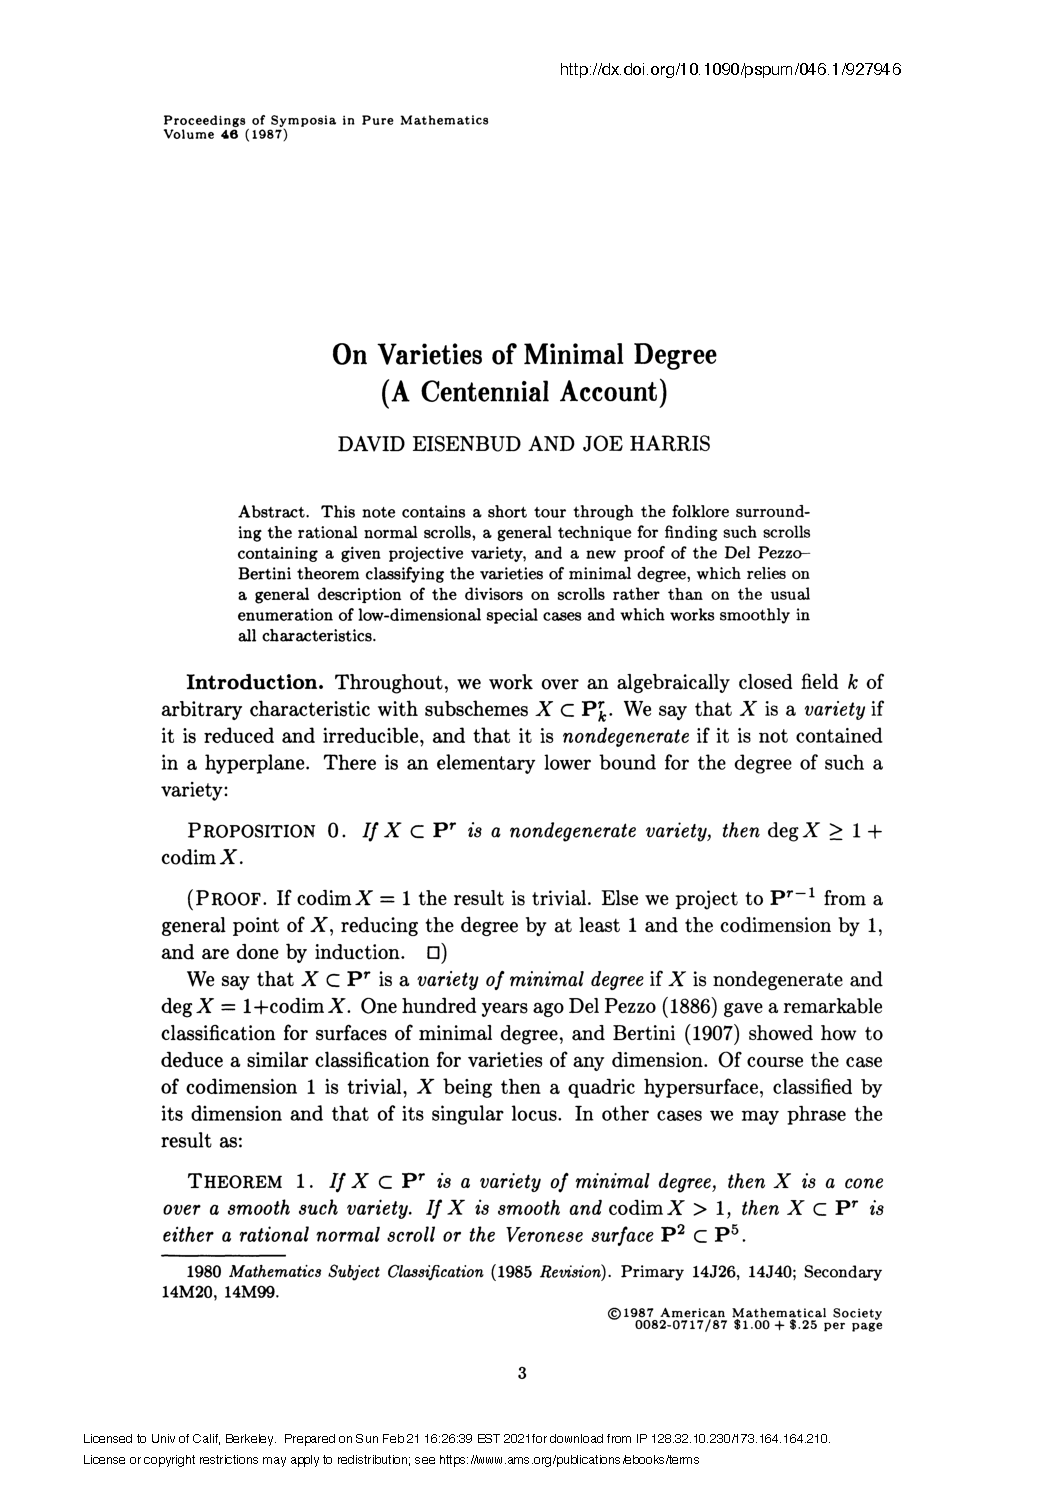
\includepdf[pages=1-11]{Centennial.pdf}


%footer for separate chapter files

\ifx\whole\undefined
%\makeatletter\def\@biblabel#1{#1]}\makeatother
\makeatletter \def\@biblabel#1{\ignorespaces} \makeatother
\bibliographystyle{msribib}
\bibliography{slag}

%%%% EXPLANATIONS:

% f and n
% some authors have all works collected at the end

\begingroup
%\catcode`\^\active
%if ^ is followed by 
% 1:  print f, gobble the following ^ and the next character
% 0:  print n, gobble the following ^
% any other letter: normal subscript
%\makeatletter
%\def^#1{\ifx1#1f\expandafter\@gobbletwo\else
%        \ifx0#1n\expandafter\expandafter\expandafter\@gobble
%        \else\sp{#1}\fi\fi}
%\makeatother
\let\moreadhoc\relax
\def\indexintro{%An author's cited works appear at the end of the
%author's entry; for conventions
%see the List of Citations on page~\pageref{loc}.  
%\smallbreak\noindent
%The letter `f' after a page number indicates a figure, `n' a footnote.
}
\printindex[gen]
\endgroup % end of \catcode
%requires makeindex
\end{document}
\else
\fi


%Let $B= \PP^{1}$, $\sE = \sO_{\PP^{1}}(a_{1}) \oplus \sO_{\PP^{1}}(a_{2})$ and  $\pi: X = \PP_{B}(\sE) \to B$ the structure map.
%
% From the general formula for the Picard group of a projective bundle above, and the fact that the Picard group of
% $\PP^{1}$ is $\ZZ$ we see that the divisor class group of $X$ is the free abelian group on the class of a divisor that belong to $\sO_{X}(1)$, namely the hyperplane section $H$, and $\pi^{*}(\sO_{\PP^{1}}(1)$, namely
% $\pi^{-1}(x)$ for any point $x\in \PP^{1}$, the fiber, proving the first formula.

%
%This is a special case of a very general situation, where, among other things, the Picard group is easy to compute, and which we now explain. 
%
%
%Recall that the projective space $\PP^{n}$ may be defined as $\Proj \Sym_{\CC}(\CC^{n+1})$. The inclusion
%of rings $\CC = \Sym_{\CC}(\CC^{n+1})_{0}\subset \Sym_{\CC}(\CC^{n+1})$ induces a structure map
%$\pi: \PP^{n}\to \Spec \CC$. 
%The variety $\PP^{n}$ comes equipped with a tautological line bundle $\sO_{\PP^{N}}(1)$, which is associated to the graded module $(\Sym_{\CC} \CC^{n+1})(1)$, and a tautological map 
%$$
%\CC^{n+1}\otimes \sO_{\PP^{N}} =\pi^{*}(\CC^{n+1}) \to \sO_{\PP^{N}}(1)
%$$
%that induces an isomorphism on global sections.
%
%\begin{fact}\label{projective space bundles}
%In an exactly parallel way, we may make a projective space bundle $\PP_B(\sE)$ over a variety $B$ from a vector bundle $\sE$ on  $B$ 
%by taking $\PP_B(\sE) = \Proj \Sym_{\sO_{B}} (\sE)$.
%The inclusion of sheaves of rings
%$\sO_{B}  = (\Sym_{\sO_{B}}(\sE))_{0} \hookrightarrow \Sym_{\sO_{B}}(\sE)$ induces a structure map
%$\pi: \PP_B(\sE) \to B$. If $\sE$ has rank $n+1$, then over any closed point $b\in B$ we have
%$\sE_{b} \cong \CC^{n+1}$, and so the fiber $\pi^{-1}(b)$ is $\PP^{N}$. The restriction of 
%$\sO_{\PP_B(\sE)}(1)$ to $\pi^{-1}(b)$ is $\PP^{N}$ is $\sO_{\PP^{N}}(1)$.
%
%The variety $\PP_{B}(\sE)$ comes equipped with a tautological line bundle $\sO_{\PP_{B}}(\sE)(1)$, which is associated to the graded module $(\Sym_{\sO_{B} (\sE)}(1)$, and a tautological map 
%$$
%\pi^{*}(\sE) \to \sO_{\PP_{B}(\sE)}(1)
%$$
%that induces an isomorphism on global sections. Furthermore, 
%$$
%\pi_{*}\sO_{\PP_{B}(\sE)}(p)) = \Sym^{p}(\sE)
%$$
%for every $p$.
%
%Thus the pair $(\PP_{B}(\sE), \sO_{\PP_{B}(\sE)}(1))$ determines $\sE$; but 
%$\PP_{B}(\sE)$ alone determines $\sE$ only up to twisting with a line bundle on $B$. For example, 
%if $\sE$ is itself a line bundle on $B$, then $\PP_{B}(\sE) \cong  B$, but $\sO_{\PP_{B}(\sE)}(1)) \cong \sE$.
%
%Conversely, if $\pi: X\to B$ is a map whose fibers are isomorphic to $\PP^{N}$, and if $X$ carries a line bundle $\sL$ whose restriction to each fiber of $\pi$ is $\sO_{\PP^{N}}(1)$, then $X\cong \PP_{B}(\sE)$ and $\sL \cong \sO_{\PP_{B}(\sE)}(1)$,
%where $\sE = \pi_{*}(\sL)$.
%\end{fact}

%
%Finally, the Picard group of invertible sheaves on $X$ is
%$\Pic X \cong \Pic B \oplus \ZZ h$, where $h$ is the class of the tautological bundle, and
%the map $\Pic B\to \Pic X$ is pull-back by $\pi$.
%The case of scrolls is the case where $B =\PP^{1}$. The situation is simpler than the general case, 
%because every vector bundle
%on $\PP^{1}$ is a sum of line bundles $\sO_{\PP^{1}}(a_{i})$. For simplicity of notation and concreteness, we will concentrate on the case of 2-dimensional scrolls. The case of $r$-dimensional scrolls is exactly parallel, and we give some references. 
% 
%Let $X := S(a_{1}, a_{2})\subset \PP^{N}$ be a nonsingular scroll of degree $a=a_{1}+a_{2}$ and $N = a_{1}+a_{2}+1$. In terms of the geometry of Section~\ref{daily name}, the variety $X$ is fibered over
%$B:=\PP^{1}$ with fibers being the lines joining the corresponding points of the directrices $C_{a_{1}}$ and 
%$C_{a_{2}}$. More precisely, in terms of the algebra of Section~\ref{particular name}, if $M$ is a
%a $2\times a$, 1-generic, matrix of linear forms
%$$
%\begin{pmatrix}
% \ell_0&\ell_{1}&\dots &\ell_{a-1}\\
% \ell_1&\ell_{2}&\dots &\ell_{a}\\ 
%\end{pmatrix}
%$$
% whose $2\times 2$ minors generate the ideal of $X$,
%then the map 
%$$
%\sO_{\PP^{N}}^{a}(-1)\to \sO_{\PP^{N}}^{2}
%$$
% defined by $M$ has rank 1 everywhere
%on $X$, so its cokernel is a line bundle $\sL$ with two global sections. The zero locus
%of the image of the first generator is the set where the second row vanishes, that is, 
%one of the planes of the scroll, and similarly for any scalar linear combination of the
%two generators; that is, $\sL$ defines a morphism $\pi: X \to \PP^{1}$ whose fibers are
%projective lines.
%
%Because the fibers of $\pi$ are embedded as linear spaces, the line bundle $\sO_{\PP^{N}}(1)$
%restricts to a line bundle on each fiber $\PP^{1}$ of $\pi$ that is the  equal to $\sO_{\PP^{1}}(1)$.
%
%
%To check these statements, we reverse the process: Let 
%$\sE =  \sO_{\PP^{1}}(a_{1}) \oplus \sO_{\PP^{1}}(a_{2})$
%and consider the complete linear series  
%$
%|\sO_{\PP_B(\sE)}(1)|.
%$
%Because $\sE$ is generated by global sections, this linear series is base point free and thus defines
%a morphism
%$$
%\phi:  \PP_B(\sE) \to \PP_B(H^{0}(\sE)) = \PP^{N}.
%$$
%
%The variety $\PP_B(\sE)$ contains subvarieties corresponding to the rank 1 quotients 
%$\sO_{\PP^{1}}(a_{i})$ of $\sE$, and the bundle $\sO_{\PP_B(\sE)}(1)$ restricts to
%the bundle $\sO_{\PP_B(\sO_{\PP^{1}}(a_{i}))}(1)$. The sections of $\sO_{\PP^{1}}(a_{i})$ restrict
%as well, and we see that the image of $\phi$ contains the rational normal curves
%$C_{a_{i}}\subset \PP^{a_{i}}$. Since all the sections from $\sO_{\PP^{1}}(a_{1})$ vanish on the $C_{a_{2}}$, and similarly for $\sO_{\PP^{1}}(a_{2})$ and $C_{a_{1}}$, we see that the two curves are embedded in  disjoint subspaces spaces. Furthermore, since the structure maps $C_{a_{i}} = \PP_{B}(\sO(a_{i})) \to \PP^{1}$ are
%isomorphisms, we see that each
% fiber of $\PP_B(\sE)$ meets each $C_{a_{i}}$ in a single point. Thus the embedded
% variety $X\subset \PP^{N}$ is a scroll, as claimed.
%
%
%
%
%Putting this together we have outlined part of the proof of the following:
%
%\begin{fact}\label{push-forward formula}
% If $X := S(a_{1}, a_{2})\subset \PP^{N}$ is a nonsingular rational normal scroll, then
% $X$ is isomorphic to a projective space bundle $\PP_{B}(\sE)$, where $B = \PP^{1}$, and the restriction of $\sO_{\PP^{N}}(1)$ to $X$
% is $\sO_{\PP_B(\sE)}(1)$. Further, writing $\pi: X\to \PP^{1}$ for the structure map, we have
%$$
%\sE = \pi_{*}(\sO_{X}(1)) = \sO_{\PP^{1}}(a_{1}) \oplus sO_{\PP^{1}}(a_{2}),
%$$
%and more generally 
%$$
%\pi_{*}(\sO_{X}(p)) = \Sym^{p}\sE = \sO_{\PP^{1}}(pa_{1}) \oplus \sO_{\PP^{1}}((p-1)a_{1}+a_{2})
%\oplus \cdots\oplus \sO_{\PP^{1}}(pa_{2}).
%$$
%
%\end{fact}
%
%In particular, since $\Pic(\PP^{1}) = \ZZ$, we see that the divisor class group
%of a scroll $S(a_{1}, a_{2})$ is freely generated by the class $H$ of a hyperplane section and the class $F$ of a ruling. The intersection form, is now easy to compute. If $C,D$ are divisor classes on the scroll, we write $C\cdot D\in \ZZ$ for their intersection number.
% 




%header and footer for separate chapter files

\ifx\whole\undefined
\documentclass[12pt, leqno]{book}
\usepackage{graphicx}
\input style-for-curves.sty
\usepackage{hyperref}
\usepackage{showkeys} %This shows the labels.
%\usepackage{SLAG,msribib,local}
%\usepackage{amsmath,amscd,amsthm,amssymb,amsxtra,latexsym,epsfig,epic,graphics}
%\usepackage[matrix,arrow,curve]{xy}
%\usepackage{graphicx}
%\usepackage{diagrams}
%
%%\usepackage{amsrefs}
%%%%%%%%%%%%%%%%%%%%%%%%%%%%%%%%%%%%%%%%%%
%%\textwidth16cm
%%\textheight20cm
%%\topmargin-2cm
%\oddsidemargin.8cm
%\evensidemargin1cm
%
%%%%%%Definitions
%\input preamble.tex
%\input style-for-curves.sty
%\def\TU{{\bf U}}
%\def\AA{{\mathbb A}}
%\def\BB{{\mathbb B}}
%\def\CC{{\mathbb C}}
%\def\QQ{{\mathbb Q}}
%\def\RR{{\mathbb R}}
%\def\facet{{\bf facet}}
%\def\image{{\rm image}}
%\def\cE{{\cal E}}
%\def\cF{{\cal F}}
%\def\cG{{\cal G}}
%\def\cH{{\cal H}}
%\def\cHom{{{\cal H}om}}
%\def\h{{\rm h}}
% \def\bs{{Boij-S\"oderberg{} }}
%
%\makeatletter
%\def\Ddots{\mathinner{\mkern1mu\raise\p@
%\vbox{\kern7\p@\hbox{.}}\mkern2mu
%\raise4\p@\hbox{.}\mkern2mu\raise7\p@\hbox{.}\mkern1mu}}
%\makeatother

%%
%\pagestyle{myheadings}

%\input style-for-curves.tex
%\documentclass{cambridge7A}
%\usepackage{hatcher_revised} 
%\usepackage{3264}
   
\errorcontextlines=1000
%\usepackage{makeidx}
\let\see\relax
\usepackage{makeidx}
\makeindex
% \index{word} in the doc; \index{variety!algebraic} gives variety, algebraic
% PUT a % after each \index{***}

\overfullrule=5pt
\catcode`\@\active
\def@{\mskip1.5mu} %produce a small space in math with an @

\title{Personalities of Curves}
\author{\copyright David Eisenbud and Joe Harris}
%%\includeonly{%
%0-intro,01-ChowRingDogma,02-FirstExamples,03-Grassmannians,04-GeneralGrassmannians
%,05-VectorBundlesAndChernClasses,06-LinesOnHypersurfaces,07-SingularElementsOfLinearSeries,
%08-ParameterSpaces,
%bib
%}

\date{\today}
%%\date{}
%\title{Curves}
%%{\normalsize ***Preliminary Version***}} 
%\author{David Eisenbud and Joe Harris }
%
%\begin{document}

\begin{document}
\maketitle

\pagenumbering{roman}
\setcounter{page}{5}
%\begin{5}
%\end{5}
\pagenumbering{arabic}
\tableofcontents
\fi


\chapter{Liaison}
\label{LiaisonChapter}


\section{Introduction} 


In studying the embeddings of a curve $C\subset \PP^r$  we have again and again estimated the number of
forms of degree $d$ in the ideal of the curve using the sequence
$$
0\to H^0(\sI_C(d)) \to H^0(\sO_{\PP^r}(d))\to  H^0(\sO_C(d)) \to H^1(\sI_C(d))\to 0
$$
which is exact because (since $r$ must be $\geq 2$ in any interesting case) $H^1(\sO_{\PP^r}(d))= 0$. In words: 
$H^1(\sI_C(d))$ measures the failure of hypersurfaces of degree $d$ to cut out a complete linear series on $C$. Curves for which
$H^1(\sI_C(d))=0$ for all $d$ are said to be \emph{arithmetically Cohen-Macaulay}; Theorem~\ref{canonical curves are ACM} shows that
all canonical curves have this property, and Theorem~\ref{high degree ACM} shows that any curve of genus $g$ embedded by a
 complete linear series of degree $\geq 2g+1$ does too.
  
In the interesting case of curves in $\PP^3$ the spaces $H^1(\sI_C(d))$ play a particularly important role that is
the subject of the theory of linkage (often called by its French name, liaison).

\section{The Cohen-Macaulay property}
A sequence of elements $f_1,\dots, f_t\in \gm$ is a \emph{regular sequence} on $M$ if $f_i$ is a nonzerodivisor on $M/(f_1, \dots, f_{i-1})M$
for $i = 1,\dots,t$. 
All maximal regular sequences on $M$ have the same length, called the \emph{depth}  $\depth M$, and 
$\depth M + \pd M = \dim R$. The depth of $M$ is always $\leq \dim M$, and in the case of equality $M$ is said to be a Cohen-Macaulay module. Every
localization of a Cohen-Macaulay module is also Cohen-Macaulay. If $M$ is and $R$-algebra, then the depth of $M$ is independent
of $R$, and if $M$ is Cohen-Macaulay we say simply that it is a Cohen-Macaulay ring. For example, any 0-dimensional module is Cohen-Macaulay,
and a 1-dimensional module is Cohen-Macaulay if and only if $\gm$ is not an associated prime of $0\subset M$; that is, if and only if $M$ is purely 1-dimensional. In particular, any purely 1-dimensional scheme is Cohen-Macaulay.

Analogous results hold over a positively graded polynomial ring such us the homogeneous coordinate ring $S = \CC[x_0,\dots,x_r]$ of $\PP^r$ when
only graded modules are considered and all elements are taken to be homogeneous. Most interesting for the purposes of this book are the
homogeneous coordinate rings $S_X$ and local rings $\sO_{X,p}$ of projective schemes $X$. If all the $\sO_X$ are Cohen-Macaulay rings then we say that
$X$ is a Cohen-Macaulay scheme. If $S_X$ is Cohen-Macaulay then we say that $X$ is \emph{arithmetically Cohen-Macaulay}. Since the $\sO_{X,p}$ can be obtained as localizations of $S_X$ the scheme, this is a stronger condition than $X$ being Cohen-Macaulay.
\begin{proposition}
If $X\subset \PP^r$ is a projective scheme then $X$ is Cohen-Macaulay if and only if 
$X$ is pure-dimensional and
$$
H^i(\sO_X(m))= 0
$$
for all $0<i<dim X$ and all $m\in \ZZ$. The scheme
 $X$ is arithmetically Cohen-Macaulay if and only if $X$ is Cohen-Macaulay and either $X$ is 0-dimensional or
$H^1(\sI_X(m))$ = 0 for all $m$.
\end{proposition}

For example, a purely 1-dimensional scheme $C$  is arithmetically Cohen-Macaulay if and only if $H^1(\sI_C(m) = 0$
for all m.
By Serre's Vanishing theorem $H^1(\sI_X(m)) = 0$ for $m\gg 0$ in any case; and if $X$ has
no 0-dimensional component then, since $H^1(\sI_X(m))$ is the cokernel of the natural map $H^0(\sO_{\PP^r}(m) \to H^0(\sO_{X}(m)$,
it vanishes for $m<0$. Thus, assuming that  $X$
no 0-dimensional component, the sum $D(X) := \oplus_{m\in \ZZ} H^1(\sI_X(m))$ is a graded $S$-module that
is a finite dimensional vector space called the \emph{Hartshorne-Rao invariant} or \emph{deficiency module} of $X$;
it is the obstruction to $X$ being arithmetically Cohen-Macaulay.


\section{Linkage of smooth curves in $\PP^3$}\label{SLinkage}\label{linkage section}

In Chapter~\ref{ModuliChapter} we considered the Hilbert scheme of twisted cubics, and proved that the open set consisting of 
smooth irreducible nondegenerate cubic curves in $\PP^3$---that is, twisted cubics---is irreducible of
dimension 12. To illustrate the technique of linkage, we give a second proof of this fact:

\begin{proof}[Second proof of Proposition~\ref{hilb of twisted cubics}]
Let $C\subset \PP^3$ be a twisted cubic. In Chapter~\ref{linear series chapter} we used the sequence
$$
0\to H^0(\sI_C(2)) 
\to H^0(\sO_{\PP^3}(2) 
\to H^0(\sO_C)
$$
To deduce that $C$ lies on at least 2 quadrics. But the intersection of any two distinct quadrics $Q, Q' \supset C$ containing a twisted cubic curve $C$ has degree 4 and is unmixed; therefore it is the union of $C$ and a line $L \subset \PP^3$.

Conversely, suppose that $L \subset \PP^3$ is any line and  $Q, Q'$ two general quadrics containing $L$; write the intersection $Q \cap Q'$ as a union $L \cup C$. Since smooth quadrics contain lines a general quadric containing $L$ is smooth. The quadric $Q'$ will intersect $Q$ in a curve of type $(2,2)$, so the curve $C$ will have class $(2,1)$ or $(1,2)$. Since $\sI_Q =\sO_{\PP^3}(-2)$, the quadrics $Q'$ containing $L$ cut out on $Q$ the complete linear system of curves of type $(2,1)$, 
 which has no base locus, so Bertini's theorem tells us that $C$ is smooth, so that the intersection $Q \cap Q' = L \cup C$ is the union of $L$ and a twisted cubic. This suggests that we set up an incidence correspondence: let $\PP^9$ denote the projective space of quadrics in $\PP^3$, and consider
$$
\Phi = \{ (C, L, Q, Q') \in \cH^\circ \times \GG(1,3) \times \PP^9 \times \PP^9 \; \mid \; Q \cap Q' = C \cup L \}.
$$

We'll analyze $\Phi$ by considering the projection maps to $\cH^\circ$ and $\GG(1,3)$; that is, by looking at the diagram

\begin{diagram}[small]
& &  \Phi & & \\
& \ldTo^{\pi_1} & & \rdTo^{\pi_2} & \\
\cH^\circ & & & & \GG(1,3)
\end{diagram}

Consider first the projection map $\pi_2 : \Phi \to \GG(1,3)$ on the second factor. By what we just said, the fiber over any point $L \in \GG(1,3)$ is an open subset of $\PP^6 \times \PP^6$, where $\PP^6$ is the space of quadrics containing $L$; it follows that $\Phi$ is irreducible of dimension $4 + 2\times 6 = 16$. Going down the other side, we see that the map $\pi_1 : \Phi \to \cH^\circ$ is surjective, with fiber over every curve $C$ an open subsets of $\PP^2 \times \PP^2$, where $\PP^{2}$ is the projective space of quadrics containing $C$; we conclude that $\cH^\circ$ is irreducible of dimension 12.
\end{proof}

As the second proof of Proposition~\ref{hilb of twisted cubics} suggests, when the union of two curves $C$ and $C'$ forms a complete intersection we can use this fact to relate the geometry of their respective Hilbert schemes. This is a technique we'll use repeatedly. We prove it first in a special case, in which little more
than the adjunction formula is needed, and then consider a natural
generalization to purely 1-dimensional subschemes.

\begin{theorem}\label{liaison genus formula-first version} Let $C, {C'}\subset \PP^3$ smooth irreducible curves of  of degrees $c,d$ whose union is the complete intersections of two surfaces $S,T$, with $S$ smooth. If the degrees of $S,T$ are $s,t$ respectively, then $\deg C+\deg C' = st$ and the genera of $C,C'$ are
related by
 $$
 g(C) - g({C'}) = \frac{s+t-4}{2}(\deg C-\deg {C'}).
 $$
\end{theorem}
In words, the difference between the genera of $C$ and ${C'}$ is proportional to the difference in their degrees, with constant of proportionality $(s+t-4)/2$.

\begin{proof}
B\'ezout's Theorem tells us that $\deg C+\deg {C'} = st$; we want a formula relating the genera $g(C)$ and $g({C'})$ of $C$ and ${C'}$. For this we use
 the intersection theory of divisors on $S$.

By the adjunction formula (Theorem ****), the canonical divisor class of $S$ is $K_S = (s - 4)H$, where $H$ denotes the hyperplane class on $S$. Using adjunction 
again, we see that
$$
2g(C)-2 = (C\cdot C) + (K_S\cdot C) = C\cdot C + (s-4)\deg C, 
$$
or in other words,
$$
(C \cdot C) = 2g(C)-2 - (s-4)\deg C.
$$
Next, since $C \cup {C'}$ is a complete intersection of $S$ with a surface of degree $t$, we have $C + {C'}\sim tH$. Thus 
$$
(C \cdot {C'}) = (C \cdot (tH - C)) = t\deg C - (C \cdot C) = t\deg C - 2g(C) + 2 + (s-4)\deg C
$$
and similarly
$$
({C'} \cdot {C'}) = ({C'} \cdot (tH - C)) = t\deg {C'} - t\deg C + 2g - 2 - (s-4)\deg C. 
$$
Finally, we can apply the adjunction formula to ${C'}$ to arrive at
$$
2g(C') - 2 = ({C'} \cdot {C'}) + (K_S \cdot {C'}) = (s-4)\deg {C'}  + t\deg {C'} - t\deg C + 2g(C) - 2 - (s-4)\deg C.
$$
Collecting terms, we can write this in the convenient form
$$
g(C)-g(C') = \frac{s+t-4}{2}(\deg {C}-\deg C').
$$
 \end{proof}

\section{Linkage of purely 1-dimensional schemes in $\PP^3$}

The first step in dealing with a more general case, where $C,{C'}$ may not be reduced or irreducible, and my share components, is to agree
on the analogue of the statement $C\cup {C'} = S\cap T$. Writing $F,G$ for the defining equations of $S,T$ respectively,
In the simple case above, the primary decomposition of the ideal $(F,G)$ was the intersection of two prime ideals $I_C+I_{C'}$. From this description it
follows that
$$
(F,G):I_C := \{H \mid HI_C \subset (F,G)\} = I_{C'}
$$
Since the associated primes of $(F,G):I_C$ are among the associated primes of $(F,G)$, 
${C'}$ is again a purely 1-dimensional scheme. 

Constructions of this type were understood by Macaulay in his great paper~\cite{Macaulay1913} or \cite{Eisenbud-Gray} for ideals in polynomial rings. For the modern theory, as
well as some of the history, see~\cite{MR0364271}.
By analogy, we will say that two purely 1-dimensional subschemes of $\PP^3$ are \emph{directly linked} by surfaces $S: \{F = 0\}$ and $T:  \{F = 0\}$ if
the equation above is satisfied, and we say that they are \emph{linked} if they are connected by a chain of direct linkages; the equivalence relation
defined in this way is called \emph{liaison}. 

Historically, the first case to be understood was that of arithmetically Cohen-Macaulay curves in $\PP^3$.



The degrees and (arithmetic) genera 
of directly linked schemes are related exactly as in the simple case above:

\begin{theorem}\label{direct linkage}
If $C\subset \PP^3$ is a purely 1-dimensional subscheme, and ${C'}$ is directly linked to $C$, then $C$ is directly linked to ${C'}$.
If $C,{C'}\subset \PP^3$ of degrees $c,d$ are directly linked by surfaces of degrees $s,t$, then 
$\deg C+\deg C' = st$ and 
 \begin{equation}\label{linked genus formula}
p_a(C) - p_a({C'}) = \frac{s+t-4}{2}(\deg C - \deg C');
\end{equation}
\end{theorem}

\begin{proof}
 
\subsubsection{\it Proof that direct linkage is symmetric:}

Finally, we will use an elementary part of duality theory: if $S$ is a regular local ring of dimension $d$
with residue field $k$ and $R = S/(f_1,\dots, f_d)$, 
so that $R$ is a 0-dimensional complete intersection, then $R$ is injective as an $R$-module (that is, $R$ is 0-dimensional  and Gorenstein).
It follows that for any ideal $J\subset R$ we have $\ann J = Hom(R/J, R)$ and every $R$-module is reflexive,
so $\ann(\ann J) = J$.

Let $X\subset \PP^3$ be the subscheme defined by the complete intersection $I_X := (F,G)$.
To prove that the relation of linkage is symmetric we work with
the homogeneous ideals $I_C$ and $I_{C'} = I_X: I_C$. 
Since $I_X$ is a complete intersection, it is unmixed of codimension 2, and it
follows that $I_{C'}$ is unmixed of codimension 2 as well.
It is clear from the definition that
$$
I_C \subset I_X:(I_X:I_C) = I_X:I_{C'}.
$$
Since $I_C$ is unmixed of codimension 2, it is enough to check the equality
after localizing at each prime $P\subset S$ of codimension 2.
Moreover, both sides contain $(I_X)_P$, so we may pass to the ring $R = S_P/(I_X)_P$.
However, this is a zero-dimensional complete intersection so $\ann_R\ann_R(J) = J$.

\subsection{Dualizing modules}
To go further, we will use some facts about the dualizing modules of Cohen-Macaulay rings that generalize this
property, which comes from the fact that a Gorenstein ring is its own dualizing module; we digress from the 
proof of Theorem{direct linkage} to establish the necessary facts.

Recall that a Noetherian local ring $(R,\gm)$ of (Krull) dimension $d$ is said to be Cohen-Macaulay if there are elements $f_1,\dots,f_d\in \gm$ such that
$f_i$ is a nonzerodivisor modulo $(f_1,\dots,f_{i-1})$ for $i =1,\dots,d$, and a Noetherian ring is Cohen-Macaulay if each of its localizations at maximal ideals
is Cohen-Macaulay. Thus, for example every unmixed ring of dimension 0 or 1 is Cohen-Macaulay, and every purely 1-dimensional scheme is locally Cohen-Macaulay,
making the condition relevant in the situation of Theorem~\ref{liaison-full version}. 

Recall that in Chapter~\ref{RR} we claimed that the canonical sheaf of a smooth curve---the sheaf of differential forms---was ``the most important invertible sheaf'' after the structure sheaf. In the general setting of Cohen-Macaulay schemes, the analogue of the canonical sheaf is called the dualizing sheaf.
The general definition of the dualizing sheaf is not very illuminating; what is useful is how it is constructed and is cohomological properties relating to duality.
However, having a definition may be comforting. 
%Note that for any coherent sheaves $\sF, \sG$ on a quasiprojective  scheme $X$ there is are natural maps
%$H^p(\sF) \times \Ext^q(\sF, \sG) \to H^{p+q)(\sG)$ (Construction: An element of $\Ext^q(\sF, \sG)$ may be represented by an exact sequence starting from
%$\sG$ and ending with $\sF$. Break this into short exact sequences and use the connecting homomorphisms in the long exact sequences for cohomology.)

\begin{definition}
Let $X$ be a projective scheme over of pure dimension $d$. The \emph{dualizing sheaf} for $X$ is a coherent sheaf $\omega_X$ 
with a map $\eta: H^d(\omega_X) \to \CC$ such that for every coherent sheaf  $\sF$ the induced map
$$
H^a(\sF) \times { \rm Ext}_X^{d-a}(\sF, \omega_X) \to H^d(\omega_X) \rTo^\eta \CC
$$
is a perfect pairing for $a=d$. 
\end{definition}


\begin{fact}
If $X$ is Cohen-Macaulay, then the duality holds for all $a$ (in the non-Cohen-Macaulay case a similar result is true if we replace $\omega_X$ by a dualizing complex
and work in the derived category.) In this case, 
$$
\sHom(\omega_X, \omega_X) = \sO \hbox{ and, if $t>0$ then } \Ext_X^{t}(\omega_X, \omega_X) = 0,
$$
(see for example~\cite[Theorem[Theorems 3.3.4 and 3.3.10d]{BrunsHerzog}) so the spectral sequence $H^p(\sExt^{d-a-p}(\omega_X, \omega_X) \Rightarrow {\rm Ext}^{d-a}(\omega_X, \omega_X)$ degenerates and shows that 
$$
{\rm Ext_X}^{d-a}(\omega_X(m), \omega_X) = H^{d-a}(Hom(\omega_X(m), \omega_X)) = H^{d-a}(\sO_X(-m))
$$
Thus, if $X$ is Cohen-Macaulay, then 
$$
\chi(\omega_X(m)) =(-1)^{\dim X}\chi(\sO_X(-m)).
$$

As the name suggests, any two canonical sheaves are isomorphic in a way compatible with the
residue maps. If $X$ is smooth then the top degree differential forms $\omega_X :=\wedge^d(\Omega_X)$,
together with the classical residue (see for example~\cite[p. 648, 708]{Griffiths-Harris1978}), is a dualizing sheaf, as implied by Serre duality. Moreover, one can construct the dualizing sheaf on a scheme
$X$ by comparing it with any scheme $Y$ whose dualizing sheaf is known, in the following sense:

\begin{theorem}\label{omega}\label{general adjunction}
Suppose that $f: X\to Y$ is a finite morphism between projective schemes $X,Y$ of pure dimensions $d,e$. If $Y$ has a dualizing sheaf $\omega_Y$,
then $\omega := \sExt_Y^{e-d}(f_*\sO_X,  \omega_Y)$, regarded as a sheaf on $X$ is a dualizing sheaf for $X$ in a way compatible with the residue maps.
Moreover, if $Y$ is smooth, then $X$ is Cohen-Macaulay if and only if $ \sExt_Y^{e-d}(f_*\sO_X,  \omega_Y)= 0$ for all $m\neq e-d$.\qed
\end{theorem}

For all this see for example \cite{AltmanKleiman}.
\end{fact}


\subsection{Continuation of the Proof of Theorem~\ref{direct linkage}}

%\subsubsection{\it Degrees of directly linked curves:}
%Let $H$ be a general hyperplane in $\PP^3$ with equation $h=0$. The degrees of $C$ and $C'$ are equal to the degrees of the finite schemes $\Gamma := C\cap H$ and
%$\Gamma' := C'\cap H$. We claim that $\Gamma$ and $\Gamma'$ are directly linked by $X\cap H$, that is,
%$$
%(\sI_X:\sI_C)+(h) = (\sI_X + (h)) : (\sI_C + (h)).
%$$
%It is enough to prove that this holds modulo $\sI_X+h = \sI_{X\cap H}$, that is,
%$$
%\frac{\omega_C+(h)}{(h)} = \omega_{C\cap H}.
%$$
%Here the denominator on the left should more properly be written as $(h)(-1)$, but for simplicity in this and what follows we ignore the twists.
%Since $h$ is a nonzerodivisor modulo $I_X$ is it a nonzerodivisor on $\omega_C \subset \sO_X$, and thus
%the left hand side is isomorphic to $\omega_C/h\omega_C$, and it suffices to show that $\omega_{C\cap H)} = \omega_C/x\omega_C$,
%which follows from Lemma~\ref{restricting omega}.
%Since $\Gamma$ is directly linked to $\Gamma'$ by forms of degree $s,t$ we have
%$\deg \sO_{\Gamma'}+\deg \omega_\Gamma  = st$. On the other hand, since $\omega_\Gamma = \Hom(\sO_\Gamma, \sO_{X\cap H}$,
%and $\sO_{X\cap H}$ is 0-dimensional and Gorenstein, we have $\deg \omega_\Gamma = \deg \sO_\Gamma$, whence
%$\deg \sO_{\Gamma'}+\deg \sO_\Gamma = st$ as required.
%
%We will use a fact about the dualizing
%\begin{lemma}\label{restricting omega} If $C$ is a purely 1-dimensional projective scheme and $H$ is a general hyperplane,
%then $\omega_{C\cap H} = \omega_C(1) \mid_H$.
%\end{lemma}
%
%\begin{proof}
%Suppose  that $C\subset \PP^n$ and write $h=0$ for the equation of $H$. Since $H$ is general there is an exact sequence
%$$
%0\rTo \sO_C(-1) \rTo^h\sO_C\rTo \sO_{C\cap H} \rTo 0
%$$
%from which we get the long exact sequence containing
%$$\
%\begin{aligned}
% \cdots &\rTo \Ext^{n-1}(\sO_{C\cap H}, \omega_{\PP^n}) \rTo \omega_C \rTo^h\omega_C(1)\rTo \omega_{C\cap H}\\ 
% &\rTo 
%\Ext^{n}(\sO_{C}, \omega_{\PP^n}) \rTo \cdots
%\end{aligned}
%$$
%Since  $\sO_{C\cap H}$ is Cohen-Macaulay of codimension $n$ and $\sO_C$ is Cohen-Macaulay of codimension $n-1$,
%both $\Ext^{n-1}(\sO_{C\cap H}, \omega_{\PP^n})$ and $\Ext^{n}(\sO_{C}, \omega_{\PP^n})$ vanish, yielding the desired relation.
%\end{proof}

\subsubsection{\it Degrees of directly linked curves:}
Let $X$ be the complete intersection of surfaces of degrees $s,t$ containing $C$, and let $S_X = S/(F,G)$ be its homogeneous coordinate ring, where
$S = \CC[x_0,\dots,x_3]$ is the homogeneous coordinate ring of $\PP^3$.
From the free resolution
$$
0\rTo S(-s-t) \rTo^{
\begin{pmatrix}
 G \\ -F
\end{pmatrix}}
 S(-s)\oplus S(-t) \rTo^{
\begin{pmatrix}
 F & G
\end{pmatrix}}
 S \rTo S/(F,G) \rTo 0
$$
 and Theorem~\ref{omega} we see that
 $$
\omega_X =  \sExt^2_C(\sO_X, \omega_{\PP^3}) =\sExt^2(\sO_X, \sO_{\PP^3}(-4)) = \sO_X(s+b-4).
 $$
Note that for any ideals $J\subset I$ in a ring $A$ we have $Hom_A(A/I, A/J) \cong (J:I)/J$, where the isomorphism
sends a homomorphism $\phi$ to the element $\phi(1)$. Again from Theorem~\ref{omega} we have 
$$
\omega_C = \Hom_X(\sO_C, \omega_X) = \Hom_X(\sO_C, \sO_X)(s+t-4) = \frac{\sI_X:\sI_C}{\sI_X}(s+t-4),
$$
where we have identified $\sO_C$ with its pushforward under the inclusion map $C\to X$. 

Since $C$ is purely 1-dimensional it is Cohen-Macaulay, so
$\chi(\omega_C(m)) = -\chi(\sO_C(-m))$. It follows that the degree of $\omega_C$, which is the leading coefficient of the Hilbert polynomial of $\omega_C$, is 
equal to $\deg C$, and 
$$
st = \deg \sO_X =\deg \sO_{C'}+\deg \omega_C = \deg \sO_{C'}+\deg \sO_C
$$
as required.

\subsubsection{\it Arithmetic genera of directly linked curves:}

From Theorem~\ref{omega} we see that $\chi(\sO_X) = st(4-s-t)/2$. Since $\sO_{C'} = \sO_{\PP^3}/(\sI_X : \sI_C)$ and
$(\sI_X : \sI_C)/(\sI_X) = \omega_C(4-s-t)$ we have
$$
\begin{aligned}
-\frac{(s+t-4)}{2} (\deg C +& \deg C') \\&= -\frac{(s+t-4)}{2}st \\
&= \chi(\sO_X) \\&=  \chi(\sO_{C'})+\chi(\omega_C(4-s-t)) \\&= \chi(\sO_{C'})-\chi(\sO_C(s+t-4)) \\&= \chi(\sO_{C'})-(s+t-4)\deg C-\chi(\sO_C)
\\&= (1-p_a(\sO_{C'})) - (1-p_a(\sO_C) -(s+t-4)\deg C,
\end{aligned}
$$
whence 
$$
p_a(\sO_C) -p_a(\sO_{C'} = \frac{(s+t-4)}{2} (\deg C - \deg C'). 
$$
 \end{proof}

Linkage behaves in a simple way with respect to deficiency modules:

\begin{theorem}\label{HR}
If $C,C'$ are purely 1-dimensional subschemes of $\PP^3$ that are directly linked by a complete intersection of degrees $s,t$ then
$$
D(C') = Hom_\CC(D(C), \CC) (-s-t+4).
$$ 
as graded modules over the homogeneous coordinate ring of $\PP^3$.
\end{theorem}

For example, the Hartshorne-Rao module of the union $C$ of two skew lines in $\PP^3$ is easily seen to be the residue field in degree 0. There are
two quadrics containing $C$, and the link with respect to these two is the union of two other skew lines, again with Hartshorne-Rao module
$k$ in degree 0.

\begin{proof}
Suppose that the homogeneous ideal of $C$ is generated by forms of degree $a_i, i=1,\dots,s$. Since $C$ is locally Cohen-Macaulay,
the local rings $\sO_{C,p}$ have projective dimension 2 as modules over $\sO_{\PP^3, p}$, and $\sI_{C,p}$ has projective dimension 1.
Thus we have an exact sequence
$$
0\to \sE \to \oplus_i\sO_{\PP^3}(-a_i) \to \sI_C \to 0.
$$
Since the first and second cohomology groups of the twists of $\sO_{\PP^3}$ vanish, we deduce an isomorphism
$$
D(C) := \oplus_{m\in \ZZ} H^1(\sI_C(m)) \cong \oplus_{m\in \ZZ} H^2(\sE(m)).
$$

Let $X$ be the complete intersection of two hypersurfaces, of degrees $s,t$, containing $C$. From the inclusion we deduce a
map of resolutions
$$
\begin{diagram}[small]
0&\rTo& \sE &\rTo& \oplus_i\sO_{\PP^3}(-a_i)                                         &\rTo&\sO_{\PP^3}&\rTo &\sO_C &\rTo& 0\\
&&\uTo&&\uTo&&\uTo&&\uTo\\
0&\rTo& \sO_{\PP^3}(-s-t) &\rTo& \sO_{\PP^3}(-s)\oplus \sO_{\PP^3}(-t) &\rTo& \sO_{\PP^3}&\rTo& \sO_X &\rTo& 0\\
\end{diagram}
$$
We dualize this diagram, form the mapping cone, and twist by $-s-t$. Note that $\Hom_{\PP^3}(\sO_C, \sO_{\PP^3}) = 0$. 
Also, since the vertical map $\sO_{\PP^3}\to \sO_{\PP^3}$ on the right
is an isomorphism we may cancel these terms. Noting that $\omega_C = \Ext^2(\sO_C, \sO_{\PP^3}(-4))$ we get the diagram with 
exact rows:
$$
\begin{diagram}[small]
 0&\lTo&\omega_C(-s-t+4)&\lTo&\sE^*(-s-t) &\lTo&  \oplus_i\sO_{\PP^3}(a_i-s-t)&\lTo&  0\\
 &&\dTo^\phi&&\dTo&&\dTo\\
 0&\lTo&\sO_X&\lTo&\sO_{\PP^3} &\lTo& \sO_{\PP^3}(-t)\oplus \sO_{\PP^3}(-s) &\lTo&0\\
 &&\dTo\\
 &&\sO_{C'}\\
 &&\dTo\\
 && 0
\end{diagram}.
$$
Here the column on the left is an exact sequence because $(\sI_X:\sI_C)/\sI_X \cong \omega_C(-s-t+4)$, as explained above.
We can now write a resolution of $\sI_{C'}$ by taking the mapping cone:
$$
\begin{diagram}
0\leftarrow \sI_{C'} \leftarrow \sO_{\PP^3}(-t)\oplus \sO_{\PP^3}(-s) \oplus \sE^*(-s-t) \leftarrow \oplus_i\sO_{\PP^3}(a_i-s-t)\leftarrow  0
\end{diagram}
$$
From this we see that 
$$
H^1(\sI_{C'}(m) \cong H^1(\sE^*(-s-t+m) \cong Hom_\CC( H^2(\sE(s+t-m-4)), \CC)
$$
where the last equality is from Serre duality on $\PP^3$. Summing over $m$ we see that
$D(C') \cong Hom(D(C)(s+t-4), \CC)$,
and since Serre duality is functorial, the isomorphism holds not only as graded vector spaces, but as graded $S$-modules. 

To prove that the relation of direct linkage is symmetric, we can repeat this argument starting from the locally free
resolution of $C'$, above, using the same forms of degree $s,t$ and we see that  direct link of $C'$ is $C$.
\end{proof}

As an immediate consequence of Theorem~\ref{HR} we have:
\begin{corollary}(Hartshorne)
 If two curves $C,C'$ are linked by an even length chain of direct linkages, then 
 $D(C)$ and $D(C')$ are isomorphic up to a shift in grading.
\end{corollary}

Remarkably, the converse is also true: the Hartshorne-Rao modules, up to shift in grading, provide a complete invariant of
linkage: 
\begin{fact}
\begin{theorem}\cite{MR520926}
Two curves $C,C'$ are linked by an even length chain of direct linkages if and only if 
the Hartshorne-Rao modules $D(C)$ and $D(C')$ are isomorphic up to a shift in grading.
\end{theorem}

Even more precise results are known (and the characteristic 0 hypothesis is largely unnecessary); here is a sample:

\begin{theorem}
Let $S = \CC[x_0, \dots, x_3]$ be the homogeneous coordinate ring of $\PP^3$, and let $M$ be a graded $S$-module of finite length.
\begin{enumerate}
\item There is a smooth curve $C$ with $D(C) = M(m)$ for some integer $m$.
\item There is a minimum value of $m$ such that $M(m) = D(C_0)$ for some purely one-dimensional scheme $C_0$.
\item Every curve that is evenly linked to $C_0$ is obtained from $C_0$ by deformation and a process called
\end{enumerate}
\end{theorem}

Moreover, each Liaison class has a relatively simple structure, known as the \emph{Lazarsfeld-Rao property}.
We say that $C'$ is obtained from $C$ by an \emph{ascending double link} if $I_{C'} = fI_C+(g)$ for some regular sequence
contained in $I_C$---see Exercise~\ref{Basic double links}. 

\begin{theorem}\cite{MR1087803}\label{LR property}
Let $M = D(C_0)$ the the Hartshorne Rao invariant of a purely 1-dimensional subscheme of $\PP^3$, and suppose that
$M$ is minimal in the sense that no $M(m)$ is the invariant of a purely 1-dimensional scheme. 
\begin{enumerate}
 \item Every curve $C$ in $\PP^3$ with $D(C) = M$ is a deformation of $C_0$ through curves with invariant $M$.
 \item Every curve in the even linkage class of $C_0$ is the result of a series of ascending double links followed by a deformation.
\end{enumerate}
\end{theorem}

In \cite{MR714753} it is shown that general curves of reasonably large degree in $\PP^3$ and many others have the property in the hypothesis
of  Theorem~\ref{LR property}.
\end{fact}


\section{Exercises}
\begin{exercise}
Let $C$ be the disjoint union of 3 skew lines. 
\begin{enumerate}
 \item prove that $C$ lies on a unique quadric, and that $H^2(\sI_C) = 0$
 \item compute the Hartshorne-Rao module $D(C)$.
 \item show that if $\Gamma$ is the union of 3 points in $\PP^3$ then
 $H^1\sI(\Gamma) = 0$ iff the three points are colinear.
 \item Using the exact sequence in cohomology coming from the short exact sequence
$$
0\to \sI_C \rTo^{\ell} \sI_C(1) \to \sI_\Gamma(1) \to 0
$$
where $\ell$ is a linear form, show that the map of vector spaces
$$
H^1(\sI_C) \rTo^{\ell} H^1\sI_C(1))
$$
has rank<2 if and only if $\ell$ vanishes on 3 collinear points on the three lines (including the case when $\ell$ vanishes identically on one of the lines).
Conclude that if a different union $C'$ of 3 skew lines is linked to $C$, then $C'$ lies on the same quadric as $C$.
\end{enumerate}
See~\cite{Migliore} for more examples of this type.
\end{exercise}

\begin{exercise} (Liaison addition)\label{Liaison addition}
(From the unpublished Brandeis thesis of Phillip Schwartau): Show that if $(f, g)\subset I\cap J$ is a regular sequence,
 then $f I \cap gJ = (fg)$, and conclude that if $I,J$ are purely codimension 2 ideals
 defining purely 1-dimensional schemes $C,C'$ in $\PP^3$
 then  $(fI+gJ)$ defines a scheme $C''$ with $D(C'') = D(C) \oplus D(C')$.
\end{exercise}

\begin{exercise}(Basic double links)\label{Basic double links}
The special case of the construction in Exercise~\ref{Liaison addition} in which $C'$ is trivial is already interesting. 

\begin{enumerate}
 \item Show that if $I$ is a purely codimension 2 ideal
 defining a purely 1-dimensional scheme $C$ in $\PP^3$
 and $(f, g)\subset I$ is a regular sequence, then
 then  $(fI+g)$ defines a scheme $C'$ with $D(C') = D(C)(-g)$.

 \item Show directly that, with notation as above, $C'$ is directly linked to $C$
 in two steps. Since the degrees of the generators of $D(C')$ are more positive, this
 is sometimes called an \emph{ascending double link}. Geometrically it amounts to taking the
 union of $C$ with some  components that are complete intersections.
 \end{enumerate}

\end{exercise}

%footer for separate chapter files

\ifx\whole\undefined
%\makeatletter\def\@biblabel#1{#1]}\makeatother
\makeatletter \def\@biblabel#1{\ignorespaces} \makeatother
\bibliographystyle{msribib}
\bibliography{slag}

%%%% EXPLANATIONS:

% f and n
% some authors have all works collected at the end

\begingroup
%\catcode`\^\active
%if ^ is followed by 
% 1:  print f, gobble the following ^ and the next character
% 0:  print n, gobble the following ^
% any other letter: normal subscript
%\makeatletter
%\def^#1{\ifx1#1f\expandafter\@gobbletwo\else
%        \ifx0#1n\expandafter\expandafter\expandafter\@gobble
%        \else\sp{#1}\fi\fi}
%\makeatother
\let\moreadhoc\relax
\def\indexintro{%An author's cited works appear at the end of the
%author's entry; for conventions
%see the List of Citations on page~\pageref{loc}.  
%\smallbreak\noindent
%The letter `f' after a page number indicates a figure, `n' a footnote.
}
\printindex[gen]
\endgroup % end of \catcode
%requires makeindex
\end{document}
\else
\fi

\begin{corollary}[Corollary of the proof of Theorem~\ref{HR}]
If $C$ is a purely 1-dimensional subscheme of $\PP^3$ with homogeneous ideal $I = I_C$ then 
$$
D(C) \cong Hom_\CC (Ext^3(S/I, S), \CC)(-4), \CC)
$$
as graded modules over the homogeneous coordinate ring $S$ of $\PP^3$.
\end{corollary}

This is a special case of the local duality isomorphism between local cohomology and the dual of Ext; see for example \cite[Theorem A.1.9]{MR2103875}.
\begin{proof}
We may choose a surjection  $\psi:  \oplus_iS(-a_i)\rTo I$, and choose the map
$\phi: \oplus_i\sO_{\PP^3}(-a_i)\rTo\sI_C$
in the proof of Theorem~\ref{HR}
to be the corresponding map of sheaves, so that
$\sE$ is the sheafification of the graded module $E = \ker \psi$.

Since $I$ is a saturated ideal,
 the depth of $S/I$ is at least 1, so $\pd\ S/I\leq 3$, and $I$ has a free resolution of the form
$$
0\rTo G \rTo F \rTo \oplus_iS(-a_i)  \rTo S\rTo S/I \rTo 0.
$$
where $G\to F$ is a free presentation of $E$. and there is an exact sequence
$$
0 \to E^* \to F^* \to G^* \to Ext^3_S(S/I, S) \to 0.
$$
Since $\sO_C$ is Cohen-Macaulay the sheafification of $Ext^3_S(S/I, S)$ is 0; that is,
$Ext^3_S(S/I, S)$ has finite length, and writing $\widetilde{(\phantom{-})}$ for the sheafification functor,
we have a short exact sequence of sheaves 
$$
0\to \sE^* \to \widetilde{F^*} \to \widetilde{G^*}\to 0.
$$
From this we see that 
$$
Ext^3_S(S/I,S) = H^1_*(\sE^*) = Hom_\CC( H^2_*(\sE(-4)),\CC) = H^1_*(\sI)(-4),
$$
proving the assertion.
\end{proof}

%header and footer for separate chapter files

\ifx\whole\undefined
\documentclass[12pt, leqno]{book}
\usepackage{graphicx}
\input style-for-curves.sty
\usepackage{hyperref}
\usepackage{showkeys} %This shows the labels.
%\usepackage{SLAG,msribib,local}
%\usepackage{amsmath,amscd,amsthm,amssymb,amsxtra,latexsym,epsfig,epic,graphics}
%\usepackage[matrix,arrow,curve]{xy}
%\usepackage{graphicx}
%\usepackage{diagrams}
%
%%\usepackage{amsrefs}
%%%%%%%%%%%%%%%%%%%%%%%%%%%%%%%%%%%%%%%%%%
%%\textwidth16cm
%%\textheight20cm
%%\topmargin-2cm
%\oddsidemargin.8cm
%\evensidemargin1cm
%
%%%%%%Definitions
%\input preamble.tex
%\input style-for-curves.sty
%\def\TU{{\bf U}}
%\def\AA{{\mathbb A}}
%\def\BB{{\mathbb B}}
%\def\CC{{\mathbb C}}
%\def\QQ{{\mathbb Q}}
%\def\RR{{\mathbb R}}
%\def\facet{{\bf facet}}
%\def\image{{\rm image}}
%\def\cE{{\cal E}}
%\def\cF{{\cal F}}
%\def\cG{{\cal G}}
%\def\cH{{\cal H}}
%\def\cHom{{{\cal H}om}}
%\def\h{{\rm h}}
% \def\bs{{Boij-S\"oderberg{} }}
%
%\makeatletter
%\def\Ddots{\mathinner{\mkern1mu\raise\p@
%\vbox{\kern7\p@\hbox{.}}\mkern2mu
%\raise4\p@\hbox{.}\mkern2mu\raise7\p@\hbox{.}\mkern1mu}}
%\makeatother

%%
%\pagestyle{myheadings}

%\input style-for-curves.tex
%\documentclass{cambridge7A}
%\usepackage{hatcher_revised} 
%\usepackage{3264}
   
\errorcontextlines=1000
%\usepackage{makeidx}
\let\see\relax
\usepackage{makeidx}
\makeindex
% \index{word} in the doc; \index{variety!algebraic} gives variety, algebraic
% PUT a % after each \index{***}

\overfullrule=5pt
\catcode`\@\active
\def@{\mskip1.5mu} %produce a small space in math with an @

\title{Personalities of Curves}
\author{\copyright David Eisenbud and Joe Harris}
%%\includeonly{%
%0-intro,01-ChowRingDogma,02-FirstExamples,03-Grassmannians,04-GeneralGrassmannians
%,05-VectorBundlesAndChernClasses,06-LinesOnHypersurfaces,07-SingularElementsOfLinearSeries,
%08-ParameterSpaces,
%bib
%}

\date{\today}
%%\date{}
%\title{Curves}
%%{\normalsize ***Preliminary Version***}} 
%\author{David Eisenbud and Joe Harris }
%
%\begin{document}

\begin{document}
\maketitle

\pagenumbering{roman}
\setcounter{page}{5}
%\begin{5}
%\end{5}
\pagenumbering{arabic}
\tableofcontents
\fi


\chapter{Syzygies}
\label{SyzygiesChapter}

%Useful for drawing betti tables:
%$$
%\vbox{\offinterlineskip %\baselineskip=15pt
%\halign{\strut\hfil# \ \vrule\quad&# \ &# \ &# \ &# \ &# \ &# \ 
%&# \ &# \ &# \ &# \ &# \ 
%\cr
%degree&\cr
%\noalign {\hrule}
%0&1&--&--&--&--&--&--\cr
%1&--&17&46&45&4&--&--\cr
%2&--&--&--&--&25&18&4\cr
%\noalign{\bigskip}
%\omit&\multispan{8}{\bf Conjectural shape of $F_\bullet$}\cr
%\noalign{\smallskip}
%}}
%$$
%
%
%\centerline{\scriptsize
%\begin{tabular}{r|ccc} 
%$j\backslash i$&0&1&2\\ 
%\hline 
%0&1&$-$&$-$\\ 
%1&$-$&3&2\\ 
%\end{tabular}}
%
%
%$$
%\begin{matrix} 
%j\backslash i&\vline&0   &  1    & \cdots & n    \cr\hline
%\vdots&\vline&\vdots&\vdots & \cdots    &\vdots     \cr 
%       0&\vline&\beta_{0,0}&\beta_{1,1}&\cdots&\beta_{n,n}\cr
%       1&\vline&\beta_{0,1}&\beta_{1,2}&\cdots&\beta_{n,n+1}\cr
%\vdots&\vline&\vdots&\vdots & \cdots    &\vdots     \cr 
%\end{matrix}
%$$         
%%
%
\def\length{{\rm length}}

%Motivation: canonical embedding turns intrinsic invariants into projective invariants. Hilbert Function. Projective Normality; Canonical Module.
%
%What are the projective invariants that correspond to Clifford index? Conjecturally, Green's conjecture. Inequality from Eagon-Northcott.
%
%Hilbert Syzygy theorem, Hilbert function derivation, Unique minimal resolution, Betti table, 
%\fix{ introduce tools as they are used}


In Chapter~\ref{linkageChapter} we studied the resolutions of curves in $\PP^3$ understanding them through their Hartshorne-Rao modules. The
simplest case was that in which the Hartshorne-Rao module vanishes, that is, the case of arithmetically Cohen-Macaulay curves.
In this chapter we will show that curves embedded by complete linear series of high degree, and also canonical curves, are arithmetically
Cohen-Macaulay. We will then introduce the Eagon-Northcott complexes, and use them to study the resolutions of canonical curves
more closely. We close by explaining Green's conjecture, which proposes a particular relationship between the intrinsic geometry
of a curve and the shape of its minimal free resolution in its canonical embedding.

\section{What is a syzygy?}
This section contains no proofs; all of the material may be found in~\cite{Eisenbud1995}.

Let $(R,\gm, k)$ be a local ring and let $M$ be a finitely generated module. A \emph{free resolution} of $M$ is an exact complex
$$
\FF: \cdots \rTo F_s \rTo^{\phi_s} F_{s-1} \rTo^{\phi_{s-1}} \cdots \rTo F_1 \rTo^{\phi_1}  F_0 \rTo M \rTo 0.
$$
The resolution is \emph{minimal} if a minimal set of generators of $F_i$ maps to a minimal set of generators of the kernel of the following map,
or equivalently (by Nakayama's Lemma) the maps in $\FF\otimes_R k$ are all 0.

The first examples of a minimal free resolution are the Koszul complexese of complete intersections $I = (f_1,\dots, f_t)$. For $t = 2,3$ these look like
$$
\begin{aligned}
 0\rTo &R \rTo^{
\begin{pmatrix}
-f_2\\f_1
\end{pmatrix}}
 R^2\rTo^{
 \begin{pmatrix}
f_1&f_2
\end{pmatrix}}
 R \rTo R/I \rTo 0\\
%%
0\rTo R \rTo^{
\begin{pmatrix}
f_1\\f_2\\f_3
\end{pmatrix}} R^3&\rTo{
\begin{pmatrix}
 0&f_3&-f_2\\
 -f_3&0&f_1\\
 f_2&-f_1&0
\end{pmatrix}}
 R^3\rTo^{
 \begin{pmatrix}
f_1&f_2&f3
\end{pmatrix}}R \rTo R/I \rTo 0
\end{aligned}
$$

Minimal free resolutions of a given module $M$ are all isomorphic, and the \emph{projective dimension}  of $M$ is their length, the number of nonzero
maps (possibly infinity). Equivalently, 
$$
\pd\ M = \max\{s \mid \Ext^s(M,k) \neq 0.
$$
Fundamental
results of Auslander, Buchsbaum and Serre say that if $R$ is \emph{regular}---that is, the Krull dimension of $R$ is equal to the minimal number
of generators of $\gm$---if and only if the minimal free resolution of the residue field is finite, in which case
the minimal free resolution of every module is finite.

\fix{perhaps add here enough assertions to compute the regularity of a canonical curve and the symmetry of its resolution:
CM imlplies that the dual of the resolution resolves $\omega$; Gorenstein means $\omega$ is invertible. This would be a quick fix
allowing the completion of section 1.6.}


\section{Curves of high degree}
Let $C$ be a smooth curve of  genus $g$. We have seen that every invertible sheaf of degree $d \geq 2g+1$ is very ample. We will now show that
such a curve,  embedded by the corresponding complete linear series, is arithmetically Cohen-Macaulay.
\begin{theorem}\label{high degree ACM}
If $C$ is a reduced irreducible projective curve, embedded by a complete linear series $D$ of degree $\geq 2p_a(C)+1$, then
$H^1(\sI_C(d) = 0$ for all $d\in \ZZ$.
\end{theorem}

\begin{proof} We do induction on $d$, noting that
For $d\leq 1$ the conclusion is immediate. Note that the complete linear series
embeds $C$ in $\PP^{d-g}$. 

The case $d=2$ requires a special argument: By Theorem~\ref{linearly general position} the $d$ points $\Gamma = C\cap H$ of a
general hyperplane section are in linearly general position, and thus impose independent conditions on quadrics
(Reason: $d\leq (2(d-g)-1)$, and if we take any point $p$ away from $\Gamma$, then the remaining points lie in a
quadric which is the union of two planes and does not contain $p$.) This implies that
the restriction map $H^0(\sO_H(2)) \to H^0(\sO_\Gamma(2))$ is surjective, whence $H^1(\sI_\Gamma(2)) = 0.$
Applying $H^1$ to exact sequence 
$$
0\to \sI_C(1) \to \sI_C(2) \to \sI_\Gamma(2) \to 0
$$
we see that $H^1(\sI_C(2))=0$.

For $d>2$ we will show that the multiplication map
$$
H^0(\sO_C(1) \otimes H^0(\sO_C(d-1)\to H^0(\sO_{C}(d))
$$
is surjective. Since the corresponding map for $\PP^3$ is surjective, this implies that
the restriction map
$H^0(\sO_{\PP^3}(d)\to H^0(\sO_{C}(d))$
is surjective, whence $H^1(\sI_{C}(d)) = 0$.

For this we will use what David Mumford refers to as the \emph{base-point-free pencil trick}:
Let $V$ be a pair of sections of $H^0(\sO_{\PP^3}(1) = H^0(\sO_C(1)$, and consider the exact sequence
$$
0\to \wedge^2V \otimes \sO_C(d-2) \to V\otimes \sO_{C}(d-1))\to \sO_{C}(d))\to 0.
$$
Applying $H^0$ and using the fact that $H^1(\sO_C(d-2)) = 0$ completes the proof.
\end{proof}



\section{Canonical Curves}
A variation of the same argument will show that
canonical curves are arithmetically Cohen-Macaulay, and thus that smooth canonical curves are projectively normal,
a result of Max Noether that we have been using ever since Section~\ref{Noether theorem section}.
The necessary modification is to replace the base-point-free pencil with one having many base points.
We follow the treatment in \cite{Schreyer}.
 
We define a \emph{canonical curve} in $\PP^{g-1}$ to be a purely one-dimensional, nondegenerate closed subscheme  such that
$$
 h^{0}(\sO_{C}) = 1,\ h^{0}(\sO_{C}(1) = g, \hbox{ and } \omega_{C} = \sO_{C}(1).
$$

Note that the first of these hypotheses implies that $C$ is connected, and the last shows that
$C$ is (locally) Gorenstein---that is, the dualizing sheaf $\omega|_C$ is invertible.

If $C$ is a reduced and irreducible curve then by Theorem~\ref{linear general position} a general hyperplane $H\subset \PP^{g-1}$
meets $C$ transversely in a set of points in linearly general position. Any subset $\Gamma$ of $g-2$ of these points will span a $g-3$-plane $\Lambda$
meeting $C$ transversely in $\Gamma$, and we call $\Lambda$ a \emph{simple $(g-2)$-secant $(g-3)$-plane}. To include more general cases we make this part of the hypothesis:

%A \emph{simple}  $m$ secant to a scheme $C\subset \PP^r$ is an $(m-1)$-dimensional plane $\Lambda\subset \PP^r$ whose intersection with
%$C$ consists of $m$ reduced points. It follows that the the hyperplanes containing $\Lambda$ then intersect the curve in an additional base-point-free pencil. In characteristic 0, such secant planes always exist for reduced, irreducible curves. More generally:
%
%\begin{lemma}
% If $C\subset \PP^n$ is a reduced, irreducible, nondegenerate curve, and $m\leq n-2$, then the linear span $L := \overline{p_1,\dots, p_m}$
% of $m$ general points of $C$ is a simple $m$-secant; that is, a plane of dimension $m-1$ such that
% $C\cap L = \{p_1,\dots,p_m\}$ scheme-theoretically.
% \end{lemma}
% 
% 
%\begin{proof}
%The plane $L$ is contained in a hyperplane $H$, and since the points are general, we may take this to be a general hyperplane. By Bertini's Theorem, $C\cap H$ is reduced, so $C\cap L$ is also reduced.
% If $C\cap L$ had length $>m$, then by Theorem~\ref{uniform position??}\fix{in ch 8-BrillNoether} every set of $m+1$ points of $C\cap H$ would be dependent,
% and the span of $C\cap H$ would thus have dimension $\leq m-1<n-1$, and we could choose a hyperplane section $C\cap H'$ with more points than $C\cap H$, which is absurd.
%\end{proof}
%
\begin{theorem}[Max Noether]\label{canonical curves are ACM}
A canonical curve in $\PP^{g-1}$ has degree $2g-2$ and arithmetic genus $g$. If the curve has a simple
$g-2$ secant $(g-3)$-plane, then it is arithmetically Cohen-Macaulay; that is,
$\HH^{1}(\sI_{C/\PP^{g-1}}(m)) = 0$ for all $m\in \ZZ$.
\end{theorem}
  
\begin{proof} 
%The Hilbert polynomial $\chi_{C}(t) = h^{0}\sO(t)-\h^{1}\sO(t)$ of $C$ has degree equal to
%$\dim C = 1$, so it is determined by two values.

To show that
$C$ is arithmetically Cohen-Macaulay we
must show that the natural maps 
$$
\HH^{0}(\sO_{\PP^{n}}(m)) \to \HH^{0}(\sO_{C}(m))
$$
are surjective for all $m\in \ZZ$. For $m=0,1$ this is immediate from the hypothesis.

For $m<0$ we must show that $H^0(\sO_C(m)=0$. Let $D$ be the intersection of $C$
with a hypersurface of degree $-m$, so that $\sO_C(-m)$ is the ideal sheaf of
$D$. By hypothesis, the vector space $\HH^{0}\sO_{C}$ is spanned by the constant functions, and these
restrict non-trivially to $\sO_{D}$, so the kernel, $\HH^{0}(\sO_{C}(-m))$, is 0 as claimed.

By induction on $m$ it now suffices to prove the surjectivity of
$$
\HH^{0}(\sO_{C}(H)) \otimes \HH^{0}(\sO_{C}(mH)) \to \HH^{0}(\sO_{C}((m+1)H))
$$
for $m\geq 1$, where $H$ is the hyperplane divisor on $C$.

%In the left-exact sequence
%$$
%0\to \HH^{0}(\sO_{C}(-m)) \to \HH^{0}(\sO_{C}) \to \HH^{0}(\sO_{D}) 
%$$
% the identity element of $\sO_{C$, regarded as a global section,
%  maps to a nonzero global section of $\sO_{D}$. From the hypothesis that $\HH^{0}(\sO_{C) = 1$
%  it now follows that $\HH^{0}(\sO_{C}(-m)) = 0$.
%
%We begin by showing that $\sO(-m)$ has no global sections for $m>0$.
%If $D$ is a divisor equivalent to $m$ times the hyperplane section, we have an exact sequence
%By hypothesis, the vector space $\HH^{0}\sO_{C}$ is spanned by the constant functions, and these
%restrict non-trivially to $\sO_{D}$, and $\HH^{0}(\sO_{C}(-m)) = 0$ as claimed.
%
%Using the Riemann-Roch Theorem we can now compute the Hilbert function $\chi_{C}(m)$:
%We have 
%\begin{align*}
% \chi_{C}(0) &= h^{0}(\sO_{C}) - h^{1}(\sO_{C}) = h^{0}(\sO_{C}) - h^{0}(\omega_{C}) = 1-g.\\
%\chi_{C}(1) &= h^{0}(\sO_{C}(1)) - h^{1}(\sO_{C}(1)^{*}\otimes \omega_{C}) = h^{0}(\omega_{C}) - h^{0}(\sO_{C}) = g-1.
%\end{align*}
%and we deduce
%$\chi_{C}(m) = (2g-2)m -g+1$, whence we see that the degree of $C$ is $2g-2$ and $\p(C) = g$ as claimed.
%
%
%For $m <0$ we must show $\HH^{0}(\sO_{C}(m))=0.$ 
%If $D$ is a divisor equivalent to $-m$ times the hyperplane section, we have an exact sequence
%$$
%0\to \HH^{0}(\sO_{C}(m)) 
%\to \HH^{0}(\sO_{C}) 
%\to \HH^{0}(\sO_{D}) \to \cdots.
%$$
 
Let $\Gamma = \sum_{i=0}^{g-3}p_i$ be the $g-2$ points of the
simple $(g-1)$-secant $(g-3)$-plane, andLet $V$ be the span of the two sections of $\omega_C = \sO_C(1)$
vanishing on $\Gamma$. Since the points $\Gamma$
are linearly independent, we may choose homogeneous coordinates $x_{i} \in \HH^{0}(\sO_{C}(1))$ so that
$x_{i}(p_{j}) \neq 0$ if and only if $i = j$. It follows that the sections
$x_{i}^{m}$ of $\sO_{C}(m)$ span $\HH^{0}(\sO_{C}(m)|_{\Gamma})$. 

Thus 
it suffices to prove the surjectivity of
$$
\HH^{0}(\sO_{C}(mH-\Gamma)) \otimes \HH^{0}(\sO_{C}(mH)) \to \HH^{0}(\sO_{C}((m+1)H-\Gamma))
$$
for  $m\geq 1$.

Now let
$V\subset \HH^{0}(\sO_{C}(H))$ be the two-dimensional subspace of linear forms vanishing on
$\Lambda$, and thus on the $p_{i}$. 

Since $H-\Gamma$ is base-point free away from $\Gamma$, the two sections of $V$
define a short exact sequence of sheaves
$$
0\to\wedge^2 V\otimes \sO_{C}((m-1)H+\Gamma)  \to V\otimes \sO_C(mH) \to  \sO_{C}((m+1)H-\Gamma)) \to 0
$$
and we must show that the right-hand map is surjective on global sections for $m\geq 1$.

For $m\geq 2$ the divisor $(m-1)H+\Gamma$ has degree $>\deg \omega$, so
$H^1(\sO_{C}((m-1)H+\Gamma)) = 0$, and the surjectivity is immediate (this is
essentially what we did when using the ``base-point-free pencil trick'' in the proof of Theorem~\ref{high degree ACM}).

We begin by computing the dimensions of the cohomology of the three sheaves in the case $m=1$.

By hypothesis
we have $h^0(\sO_C) = 1$ and $h^0(\omega_C) = g$, so by duality
$\chi(\sO_C) = 1 - h^0(\omega_C)= 1-g$ and thus $\chi(\omega_C) = g-1$ Using this and the Riemann-Roch theorem we get
$g-1 = \chi(\omega_C) = \deg \omega_C + 1-g$, so $\deg \omega_C = \deg C = 2g-2$, just as in the smooth case.

Since $C$ is 1-dimensional the Hilbert polynomial $p(m) := \chi(\sO_C(m))$ is linear and is determined by the values
$p(0) = 1-g$ and $p(1) = g-1$ just determined, so $p(m) = (2g-2)m+1-g$. Since the points of $\Gamma$ impose
independent conditions we have 
$$
h^0(\sO_C(2H-\Gamma)) = 3g-3 - (g-2) = 2g-1.
$$ 
On the other hand,
$$
h^0(\sO_C(\Gamma)))=\deg \Gamma -g+1+h^0(H-\Gamma) = -1 + h^0(\sO_C(H-\Gamma)) = 1
$$
and 
$$
\dim V \otimes H^0(\sO_C(H)) = 2g
$$
so
$$
0\to H^0(\sO_{C}(\Gamma)  \to V\otimes H^0(\sO_C(H)) \to H^0( \sO_{C}((2)H-\Gamma))) 
$$
is right exact, as required for the case $m=1$.
\end{proof}

\begin{corollary}\label{canonical hilbert function}
If $C\subset \PP^{g-1}$ is a canonical curve with a simple $g-3$-secant, then the Hilbert function of the homogeneous coordinate ring $S_{C}$ of  $C$ depends only on $g$, and is given by:
$$
\dim({S_{C}})_{d} = h^{0}(\cO_{C}(d)) = 
\begin{cases}
 0 &\mbox {if } d<0\\
 1 & \mbox {if }  d=0\\
 g & \mbox {if }  d=1\\
 (2n-1)g+1 & \mbox {if }  d>1\\
\end{cases}
$$
\end{corollary}
\begin{proof}
By Theorem~\ref{canonical curves are ACM} implies, in particular, that the homogeneous coordinate ring of $C$ can be identified with $\oplus_{n\in \ZZ}\HH^0\sO_C(n)$.  
\end{proof}

\section{How syzygies can reflect geometry}\label{syzy and geom}

One of the main ways in which syzygies can be seen to reflect the geometry of a scheme $C\subset \PP^r$
depends on the possibility of factoring the line bundle $\sO_C(1)$ as the tensor product of two bundles on $C$
both of which have at least two independent global sections. Suppose for example that $C$ is nondegenerate, 
so that  $\sO_C(1) = \sL_1\otimes \sL_2$. Choose $m\geq 2$ independent global sections
$\sigma_1, \sigma_2$ of  $H^0(\sL_1)$ and $n\geq 2$ independent global sections $\tau_1,\dots, \tau_n$ of $H^0(\sL_2)$. Set
$$
l_{i,j}= \sigma_i\tensor \tau_j \in H^0(\sO_C(1)) = H^0(\sO_{\PP^r}(1))
$$ and consider the matrix 
$$
M = 
\begin{pmatrix}
 l_{1,1}&l_{1,2}&\dots&l_{1,n}\\
 \cdots&\cdots&\cdots&\cdots\\
  l_{m,1}&l_{m,2}&\dots&l_{m,n}
\end{pmatrix},
$$
which we think of as an $m\times n$ matrix of linear forms on $\PP^r$.

We claim that  the $2\times 2$ minors $l_{\ell,j} l_{\ell',j'}-l_{\ell,j'} l_{\ell',j}$ are in the homogeneous ideal of $I_C$ of $C$ in $\PP^r$. 
To see this,
let $\kappa$ be the ring of rational functions on $C$. Choosing identifications $\sL_i\otimes \kappa  \cong \kappa $ we see that the $\sigma_i$ and the $\tau_j$ commute with each other as elements of $\kappa  \otimes_{\sO_X} \kappa $, and thus 
$$
\bigl(l_{1,j} l_{2,j'}-l_{1,j'}l_{2,j}\bigr)|_C = \sigma_1\tau_j\sigma_2\tau_j' - \sigma_1\tau_j'\sigma_2\tau_j =0.
$$

\begin{example}
The most familiar example is that of the twisted cubic. In this case the global sections $x_0\dots x_3$ of $\sO_C(1)$ may be identified with the forms $s^3, s^2t, st^2, t^3 \in k[s,t]$, and if $p\in C \cong \PP^1$ then the multiplication of sections
in the factorization  $\sO_C(1) = \sO_C(p) \otimes \sO_C(2p)$ 
$$
\bordermatrix{
 &s^2&st&t^2\cr
 s& s^3&s^2t&st^2\cr
 t& s^2t&st^2&t^3
}
$$
 leads to the familiar matrix
$$
\begin{pmatrix}
x_0&x_1&x_2\\
x_1&x_2&x_3 
\end{pmatrix}.
$$
We have $I_2(M) = I_C$, and the same idea works for any Veronese or Segre variety.
\end{example}

In case $C$ is reduced and irreducible the matrix above has a special property: $\kappa $ is a domain, so no product of a nonzero
section of $\sL_1$ with a nonzero section of $\sL_2$ can be zero. We can state this without any reference to $C$:

\begin{definition}
Let $R$ be a commutative ring. A map $M:R^n\to R^m$ is 1-generic if the kernel of the corresponding
 map $R^{n}\otimes R^{m*} \to R$  contains no pure tensor $a\otimes b$. In more concrete terms, a matrix
$M$ is \emph{1-generic} if there are no invertible matrices $A,B$ such that  $AMB$ has some entry equal to 0.
\end{definition}

The case $m=2$, leading to a $2\times m$ matrix is the most interesting, because, as shown in Chapter~\ref{scrolls}, the ideal $I_2(M)$ of a 1-generic matrix of linear forms is the homogeneous ideal of a rational normal 
scroll a variety of of codimension $n-1$ and degree $n$. 

Moreover, the minimal free resolution of $I_2(M)$ has a special form called the 
Eagon-Northcott complex (Theorem~\ref{Eagon-Northcott}), which will appear as a subcomplex of the minimal free resolution of $I_C$. The presence of such a variety containing $C$ or
a subcomplex of this special form in the minimal free resolution of $C$ is thus necessary for the 
factorization of the line bundle $\sO_C(1)$ as above, and it is sometimes sufficient, as well.

\section{The Eagon-Northcott Complex of a $2\times n$ matrix of linear forms}

The Eagon-Northcott complex is a complex of free modules associated to any matrix over any commutative ring. The most familiar special case is the Koszul complex, which one may think of as the Eagon-Northcott complex of a $1\times n$ matrix, and  even in the general case the Eagon-Northcott complex is in a sense built out of the Koszul complexes. A full treatment of this and a whole family of related complexes can be found in 
\cite[Appendix A2]{Eisenbud1995}, and, from a more conceptual and general point of view, in \cite{Weyman-book}. Here we will only
make use of the case of a matrix such as the one above, we will present a simplified account in that case only. Here is the result we need:

\begin{theorem}\label{Eagon-Northcott}
 Let $S = k[x_0,\dots, x_r]$ be a polynomial ring,  and let $M: F\to G$ be a homomorphism with
 $F = S^n(-1), G= S^2$. If $M$ is 1-generic, then the minimal free resolution of $S/I_2(M)$ has the form:
\begin{align*}
EN(M) := 
S \lTo{\bigwedge^2 M} 
 \bigwedge^2 F&
 \lTo^{\delta_{2}}
 S^{2*}\otimes \bigwedge^3 F  \lTo^{\delta_{3}}
  (\Sym^2S^{2})^*\otimes\bigwedge^4F  \\
 &\lTo^{\delta_{4}}\cdots\lTo^{\delta_{n-1}} 
(\Sym^{n-2}S^{2})^*\otimes\bigwedge^nF 
 \lTo 0.
\end{align*}
\end{theorem}

\begin{proof} We first show that $r\geq n$; more precisely, we show that the span of the entries of $M$ has dimension $\geq n+1$. As noted above, to say that the $2\times n$ matrix of linear forms $M$ is 1-generic means that
the kernel of the corresponding map $ \phi: k^2\otimes k^n \to S_1$ contains no pure tensors. In the projective
space $\PP^{2n-1} = \PP(k^2\otimes k^n)$ the pure tensors form a variety isomorphic to $\PP^1\times \PP^{n-1}$, and thus of dimension $n$. Consequently the kernel of $\phi$ can have dimension at most $n-1$, whence the image of $\phi$ 
in $S_1 = k^{r+1}$ has dimension at least $2n-(n-1) = n+1$. 

We begin the discussion of $EN(M)$ by defining the maps $\delta_i$ and and proving that the given sequence is indeed a complex---that is, consecutive maps compose to 0. For simplicity of notation, we choose a generator of $\wedge^2 S^2$
 and identify it with $S$, which gives a sense to the map labeled $\bigwedge^2M$.
 
  Although it is not hard to do this directly, the dual maps
 $$
 \partial_i: \Sym^{i-2} G \otimes \bigwedge^i F^* \rTo \Sym^{i-1} G \otimes \bigwedge^{i+1} F^*
 $$
 have a more familar-looking description, so we define these instead. Indeed, the map $M$ corresponds to an
 element $\mu\in G\otimes F^*$. We may think of $ \Sym^{i-2} G \otimes \bigwedge^i  F^*$
 as a (bigraded) component of the exterior algebra over $ \Sym G$ of 
 $$
  \Sym G \otimes \bigwedge_S  F^*= \bigwedge_{ \Sym G} (\Sym G \otimes  F^*).
 $$
We define $\partial_i$ to be  multiplication by $\mu$ in the sense of this exterior algebra. Since $\mu$ has degree 1
in this sense, its square is 0. 

To show that $(\bigwedge^2 M)\circ \delta_2$ is zero, it is simplest to choose a matrix representing $M$.
Direct computation using only the usual expansion of a determinant
along a row shows that, up to sign,
pure basis vector $e\otimes f_i\wedge f_j\wedge f_k$ of $G^*\otimes \bigwedge^3 F$
maps under the composition $(\bigwedge^2) M\circ \delta_2$ to the determinant
of the $3\times 3$ matrix obtained from $M$ by repeating the row corresponding to $e$ and
the columns $i,j,k$. This determinant is 0 because it has a repeated row.

We next prove the split exactness of a complex of the form $EN(M')$ where $M'$ is surjective, so that we
may write $F = G\oplus F'$ and the map $M': G\oplus F' \to G$ as projection on the first factor. 
Of course
it suffices to prove the split exactness of the dual sequence, $EN(M')^*$:
\begin{align*}
EN(M')^* := 
S \rTo{\bigwedge^2 M'^*} 
 \bigwedge^2 F^*&
 \rTo^{\partial_{2}}
 G\otimes \bigwedge^3 F^*  
 \rTo^{\partial_{3}}
  \Sym^2G\otimes\bigwedge^4F^*  \\
 &\rTo^{\partial_{4}}\cdots\rTo^{\partial_{n-1}} 
\Sym^{n-2}G\otimes\bigwedge^nF^* 
 \rTo 0.
\end{align*}
In this case the proof
is an exercise in multilinear algebra. 
We begin by proving split exactness at the 
positions $\Sym^{i} G \otimes \bigwedge^{i+2}  F^*$ where $i\geq 1$.

The module
$ \Sym^{i} G \otimes \bigwedge^{i+2}  F^*$
decomposes as
\begin{align*}
&\Sym^{i} G \otimes \bigwedge^2 G^* \otimes \bigwedge^{i} F'^*\oplus \\
&\Sym^{i} G \otimes  G^*\otimes \bigwedge^{i+1} F'^* \oplus \\
&\Sym^{i} G \otimes  \bigwedge^{i+2} F'^* 
\end{align*}
Note that under our hypothesis, the element $\mu' \in G\otimes F^* = G\otimes G^* \oplus G\otimes F'^*$
has the form $(\mu_G, 0)$, where $\mu_G$ represents the identity map $G \to G$. Thus the complex
$EN(M')^*$ is a direct sum over $i$ of 3-term complexes of the form
%$$
%\Sym^{i+1} G \otimes \bigwedge^2 G^* 
%\lTo^{-\wedge \mu'} 
%\Sym^{i} G \otimes  G^*
%\lTo^{-\wedge \mu'} 
%\Sym^{i-1} G
%$$
$$
\Sym^{i-1} G 
\rTo^{-\wedge \mu'} 
\Sym^{i} G \otimes  G^*
\rTo^{-\wedge \mu'} 
\Sym^{i+1} G \otimes \bigwedge^2 G^* 
$$
tensored with various $\bigwedge^j F'^*$, and it suffices to show that the former are split exact when
$i\geq 0$. Now $\Sym G$ may be identified with $R:= S[x,y]$, where $x,y$ are a basis of $S^2$, and
as such the sequences above may be identified with components of the Koszul complex of $x,y$ over $R$,
%$$
%R\otimes \wedge^2 G\lTo R\otimes G \lTo R .
%$$
$$
0\to R \rTo R\otimes G \rTo R\otimes \wedge^2 G
$$
The only homology of this sequence is $R/(x,y)R$ at the right so if we replace  $R\otimes \wedge^2 G \cong R$ by the ideal $(x,y)R$, this sequence is a split exact sequence of free $S$-modules. This is the desired result.

It remains to treat the beginning of the complex $EN(M')^*$,
$$
S \rTo{\bigwedge^2 M'^*} 
 \bigwedge^2 F^*
 \rTo^{-\wedge \mu'}
G\otimes \bigwedge^3 F^*
$$
which, in our case, may be written:
%$$
%\wedge^2 F^* = \bigwedge^2 G^* \oplus (G^*\otimes F'^*) \oplus \bigwedge^2 F'*
%$$
%Consider the pair of maps
\begin{align*}
S \rTo{\bigwedge^2 M'^*} 
 &\bigwedge^2 G^* \ \oplus\ (G^*\otimes F'^*)\ \oplus\ \bigwedge^2 F'^*
 \rTo^{-\wedge \mu'} \\
 &G\otimes \bigwedge^2 G^*\otimes F'^*\ \oplus\ (G\otimes G^*\otimes \bigwedge^2 F'^*)\ \oplus\ G\otimes \bigwedge^3 F'^*
\end{align*}
The map $\bigwedge^2 M'$ is the projection to $\bigwedge^2 G$ composed with the chosen isomorphism
$\bigwedge^2 G \cong S$, and is thus a split monomorphism. To complete the argument, we must show that
 the map marked $-\wedge \mu'$ is a monomorphism on $(G^*\otimes F'^*) \oplus \bigwedge^2 F'^*$.
 But this map is the direct sum of the two maps
  $$
 (G^* \rTo^{-\wedge \mu'} G\otimes \bigwedge^2 G^*)  \otimes F'^*
 $$
 and
 $$
(S  \rTo^{\mu'} G\otimes G^*) \otimes \bigwedge^2 F'^*
 $$
 which are evidently split monomorphisms. 
completing the proof of split exactness of $EN(M')^*$ and thus of $EN(M')$.


To go further we use a basic result, proven in a more general form (and with a slightly different statement) in \cite[Theorem 20.9]{Eisenbud1995}. We make the convention
that the codimension of the empty set is infinity.

\begin{theorem}\label{WMACE}
 Let $S = k[x_0,\dots, x_r]$, and
 $$ 
\FF:  F_0\lTo^{\phi_1}F_1 \lTo \cdots \lTo F_{n-1}\lTo^{\phi_n} F_n\lTo 0
 $$
be a finite complex of free $S$-modules. Set
$$
X_i = \{p\in \AA^{n+1} \mid  H_i(\FF \otimes \kappa(p)) \neq 0\}
$$
The complex $\FF$ is \emph{acyclic} (that is, $H_i(\FF) = 0$ for all $i>0$) if and only if
$$
\codim X_i \geq i
$$
for all $i>0$. Moreover, $X_{0}\supseteq X_{1}\supseteq \cdots \supseteq X_{n}$
\qed
\end{theorem}

For example, Nakayama's Lemma implies that $X_{0}$ is the support of $\coker \phi_{1}$; thus $X_{0}$ is the set defined by the $\rank F_{0}$-sized minors of $\phi_{1}$. Similarly, 
and that $X_{n}$ is the support of the cokernel of the dual of $\phi_{n}$. 

Also, if $n=1$, the theorem simply says that a map $F_1\to F_0$ is a monomorphism iff it becomes a monomorphism after tensoring with the field of rational functions $K$, which follows from the flatness of
localization and the fact that $F_1$ is torsion-free, so that
$F_1 \subset F_1 \otimes K$. 

\begin{fact}
Theorem~\ref{WMACE} is true in this form over any Cohen-Macaulay ring; for more general
rings, ``codimension'' must be replaced by ``grade'', as in the given reference.
The Theorem can be generalized
to case where the $F_i$ are not free, but are sufficiently ``like'' free modules, too.
\end{fact}

Conclusion of the proof of Theorem~\ref{Eagon-Northcott}.
Let $X_{i}\subset \AA^{r+1}$ be the variety defined from the complex $EN(M)$ as in 
Theorem~\ref{WMACE}. Since $EN(M)$ becomes split exact after inverting any $2\times 2$ minor of $M$
$X_{i}$ is
contained in the closed set defined by $I_{2}(M)$, for all $i$. Thus if $I_{2}(M)$ has codimension $n-1$,
then $EN(M)$ is acyclic. 
\end {proof}

%\fix{START COMMENTED OUT MATERIAL}
%We will also use a special case of the Auslander-Buchsbaum formula connecting projective dimension and depth:
%
%\begin{theorem}\label{Auslander-Buchsbaum}
%If $R$ is a regular local ring of dimension $d$, and $M$ is a finitely generated $R$-module, then the projective dimension of $M$ is $\leq d$ with equality only if
%$M$ contains a submodule of finite length. 
%\end{theorem}
%
%\begin{corollary}\label{associated primes}
%If $R$ is a regular local ring of dimension $d$, and $M$ is a finitely generated $R$-module, then the codimension of an associated prime of $A$ is at most the projective dimension of $A$. 
%\end{corollary}
%\begin{proof}[Proof of  Corollary~\ref{associated primes}]
% Projective dimension can only decrease under localization, and
% the associated primes $P$ of $A$ are those for which $A_{P}$ contains a submodule
% of finite length.
%\end{proof}
%
%With this and the multi-linear algebra above we can  prove the basic acyclicity result for an Eagon-Northcott complex:
%
%\fix{the Theorem as now stated doesn't need the following. I've copied the short proof
%of acyclicity into the end of the proof above.}
%\begin{proposition}\label{acyclicity}
%Let $S = k[x_0,\dots, x_r]$ be a polynomial ring,  and let $M: F\to G$ be a homomorphism with
% $F = S^n(-1), G= S^2$.
% $$
% S^n \cong F \rTo^M G \cong S^2
% $$
% is a (not necessarily homogeneous) map of free $S$-modules.
% The Eagon-Northcott complex $EN(M)$ is acyclic if and only if $\codim I_2(M) \geq n-1$, in which case the dual complex is also acyclic and
% the associated primes of $I_2(M)$ are all minimal and of codimension $n-1$.
% \end{proposition}
%
%\begin{proof}[Proof of Proposition~\ref{acyclicity}]
%Let $X_{i}\subset \AA^{r+1}$ be the variety defined from the complex $EN(M)$ as in 
%Theorem~\ref{WMACE}. Since $EN(M)$ becomes split exact after inverting any $2\times 2$ minor of $M$
%$X_{i}$ is
%contained in the closed set defined by $I_{2}(M)$, for all $i$. Thus if $I_{2}(M)$ has codimension $n-1$,
%then $EN(M)$ is acyclic. 
%
%In this case the projective dimension
%of $S/I_{2}(M)$ is $n-1$, so all the associated primes of $I_{2}(M)$ have codimension
%exactly $n-1$.
%
%If $EN(M)$ is  acylic then, by Theorem~\ref{WMACE}, the codimension of $X_{n-1}$ is at least $n-1$. Thus to prove that the acyclicity of $EN(M)$ implies  $\codim I_{2}(M) \geq n-1$ (and thus
%$\codim I_{2}(M))  n-1$, it suffices to show that $X_{n-1} = X_{0}$ as algebraic sets.
%
%To see this, note that
%the ideal of $2\times 2$ minors of $M$. By definition, $X_{n-1}$ 
%is the set of points $p$ where $\kappa(p)\otimes \delta_{n-1}$ is not an inclusion, 
%or equivalently, that 
%that 
%$$
%\kappa(p)\otimes F\otimes \Sym^{n-3}G 
%\cong 
%\kappa(p)\otimes \bigwedge^{n-1} F^{*} \otimes  \Sym^{n-3}G 
%\rTo^{\partial_{n-1}}
%\kappa(p)\otimes \bigwedge^{n} F^{*} \otimes  \Sym^{n-2}G
%\cong
%\kappa(p)\otimes \Sym^{n-2}G
%$$
%is not a split surjection, and it is easy to see that the composite map takes
%$a\otimes b$ to $\kappa(p) \otimes M(a)\cdot b$, so the cokernel is the $(n-2)$-nd symmetric power
%of the cokernel of the map $\kappa(p) \otimes M$. Thus $X_{n}$ is equal to the support
%of the cokernel of $M$ itself. 
%
%By Nakayama's Lemma, $X_{0}$ is the support of $M$; furthermore, the localization of $\coker M$ at $p$ is 0 if and only if
%one of the 
%$2\times 2$ minors of $M$ is a unit locally at $p$ so $X_{0}$, so this is defined
%set-theoretically by $I_{2}(M)$.
%
%It now follows from Theorem~\ref{WMACE} that all the $X_{i}$ are equal, so $EN(M)$ is 
%acyclic if and only if $EN(M)^{*}$ is acyclic. 
%
%Since $M$ is 1-generic the entries of of the second row of $M$ are linearly independent, and since the dimension of the span of all the linear forms is at least $n+1$, some element in the first row is outside the span of the the elements in the second. After a permutation of columns we may assume that $l_{1,1}, l_{2,1}, l_{2,2},\dots l_{2,n}$ are linearly independent, and we may take them to be a subset of the variables, say $x_{0},\dots x_{n+1}$
%
%We next show by induction on $n$ that  $I_{2}(M)$ is prime. In the case $n=2$ we have $I_{2}(M) =  (x_{0}x_{2}-x_{1}l_{1,2})$ which obviously does not factor. 
%
%Now suppose that $n>2$, and let $M'$ be the matrix $M$ with the first column omitted. we know by induction that $I_{2}(M')$ is prime of codimension $n-2$. Since $I:=I_{2}(M)$ does not have the maximal ideal as an associated prime, it is saturated. The ideal $I_{2}(M)+x_{0}$ properly contains $I_{2}(M')$ and thus has codimension $\geq n-1$ in $S/x_{0}$, whence we see that every component of $I_{2}(M)$ meets the open set
%$x_{0} = 1$. Restricting to this open set \fix{complete the proof}
%\end{proof}
%
%The first non-trivial example of a finite free resolution is the Koszul complex on 3 variables, which is the minimal $S = k[x,y,z]$-free resolution of the module $S/(x,y,z)$:
%$$
%0\to S(-3) \rTo^{
%\begin{pmatrix}
%x\\y\\z 
%\end{pmatrix}}
% S^3(-2) \rTo^{\begin{pmatrix}
%0&-z&y\\
%z&0&-x\\
%-y&x &0
%\end{pmatrix}}
%S^3(-1) \rTo^{
%\begin{pmatrix}
%x&y&z
%\end{pmatrix}}
%S
%$$
%In fact this is the first example that 
%Hilbert
% presented in his famous paper \cite{Hilbert1890}. 																											
%\fix{END COMMENTED OUT MATERIAL}

\section{Betti tables of canonical curves}
\fix{We need to add the regularity of the canonical curve = 3; that plus Gorenstein, self-dual resolution,
gives the shape of the Betti table in which you could look for invariants. Gorenstein comes from the $H^{1}I$
computation. In the homol alg appendix we should explain the resolution duality, apply it here.}


\section{Syzygies and the Clifford index}


Corollary~\ref{canonical hilbert function} implies that the dimension of the vector space of forms of degree $d$
vanishing on a canonical curve is independent of the curve; for example, for $d=2$ we get
$
\dim ({I_{C}})_{2} = {g-2\choose 2}
$
The next question one might ask is whether or not these quadric generate the ideal $I_{C}$, and (much) more generally, what is the 
Betti table of the homogeneous coordinate ring of $C$.

 For example,
when $C$ is trigonal, with a $g^{1}_{3}$ defined by a line bundle $\sL$, the complementary linear series,
defined by $\omega_{C}\otimes \sL^{-1}$ has $g-2$ sections, and we see from Theorem ****
that $C$ lies on the ${g-2\choose 2}$ quadrics defined by the minors of a $2\times g-2$, 1-generic matrix of linear forms. The exactness of the Eagon-Northcott complex associated to this matrix shows that there are no relations of degree 0 on these minors -- that is, they are linearly independent over the ground field. It follows that they generate the vector space of all quadrics containing $C$. But by **** the locus defined by
the ideal of minors is a rational normal scroll of dimension 2, and thus the minors cannot generate $I_{C}$.

Furthermore, if $g = 6$ and $C$ is isomorphic to a plane quintic curve, then the canonical series of the plane quintic is $5-3 = 2$ times the hyperplane series, and it follows that the canonical image of $C$ lies on the Veronese surface in $\PP^{5}$. Using Theorem *** again, we see that the Veronese is contained in (in fact, equal to) the intersection of the quadrics defined by the $2\times 2$ minors of a generic symmetric matrix, coming from the 
multiplication map 
$$
\HH^{0}(\sO_{\PP^{1}}(1))\otimes \HH^{0}(\sO_{\PP^{1}}(1)) \to \HH^{0}(\sO_{\PP^{1}}(2)) = \HH^{0}(\sO_{\PP^{5}}(1))
$$
and there are $6 = {g-2\choose 2}$ independent quadrics in this ideal. Again in this case, they cannot generate the ideal of the curve.

One might fear that this is the beginning of some long series of examples, but in fact it is not: 

\begin{theorem} [Petri]
The ideal of a canonical curve of genus $\geq 5$ is generated by the $\g-2\choose 2$-dimensional space of quadrics it contains unless the curve is either trigonal or isomorphic to a plane quintic; in the latter cases, the ideal of the curve is generated by quadrics and cubics.
\end{theorem}

For a modern treatment of Petri's Theorem in this level of generality see \cite{Schreyer}; for a different treatment see \cite{Arbarello-Sernesi}.

The two exceptions can be described simultaneously by using the Clifford index:

\begin{definition}
 The Clifford index Cliff $\sL$ of a line bundle $\sL$ on a curve $C$ is $d-2r$, where $d := \deg \sL$ and $r :=  h^0(\sL)-1$. The Clifford index Cliff $C$ of
 a curve $C$ of genus $\geq 2$ is the minimum of the Clifford indices of special line bundles with at least 2 sections.
\end{definition}

Cliffords Theorem \ref{****} says that Cliff $C \geq 0$, and that Cliff $C = 0$ if and only if $C$ is hyperelliptic. If $C$ is not hyperelliptic, then it turns out that Cliff $C=1$ if and only if $C$ is either trigonal or isomorphic to a plane quintic. The Clifford index of any smooth curve of genus $g\geq 2$ is $\leq \lceil g/2\rceil+1$, with equality for a general curve, as one sees from the Brill-Noether Theorem~\ref{}, and for ``most'' curves the line bundle $\sL$ of maximal Clifford index has only 2 sections, though there is an infinite sequence of examples where this
``Clifford dimension'' is greater.

Moving to cubic forms, we see that $\dim ({I_C})_3 = {g+2\choose 3}-(5g-5)$. Comparing this number with the number of (possibly linearly dependent)
cubics obtained by multiplying $g$ linear forms and ${g-2\choose 2}$ quadrics, we see that the ideal of the curve has at least
$$
{g-2\choose 2} - {g+2\choose 3}-(5g-5) 
$$
independent syzygies of total degree 3 (that is, linear syzygies on the quadrics. For example when $g=4$ so that $C\subset \PP^3$ there is one quadric and 5 independent
cubics, at most 4 of which are multiples of the quadric. Since the curve has degree $6 = 2\times 3$, the ideal of the curve must be generated by
the quadric and one cubic. When $g=5$ there are genuinely two possibilities: the three quadrics in the ideal might be a complete intersection
(then they generate the ideal), so the Betti table would be

\centerline{\small %\scriptsize
\begin{tabular}{r|ccc} 
$j\backslash i$&0&1&2\\ 
\hline 
0&1&$-$&$-$\\ 
1&$-$&2&$-$\\ 
2&$-$&$-$&$1$\\ 
\end{tabular}}

\noindent or the curve could be trigonal, in which case the 3 quadrics generate the ideal of a surface scroll $F$. In the latter
case, the Eagon-Northcott complex resolves the homogeneous coordinate  ring  $S_F$ of the scroll,
$$
0\to S^2(-3) \to S^3(-2) \to S \to S_F \to 0
$$
which has Betti table

\centerline{\small %\scriptsize
\begin{tabular}{r|ccc} 
$j\backslash i$&0&1&2\\ 
\hline 
0&1&$-$&$-$\\ 
1&$-$&3&$2$\\ 
\end{tabular}}
\noindent and we see that there are 2 linear relations among the quadrics. Thus the minimal generators of $I_C$ must include exactly 2 cubics as well as the 3 quadrics. Since the homogeneous ring of a canonical curve is Gorenstein, its minimal free resolution is symmetric, and this is enough for us to fill in its Betti table:

\centerline{\small %\scriptsize
\begin{tabular}{r|cccc} 
$j\backslash i$&0&1&2&3\\ 
\hline 
0&1&$-$&$-$&$-$\\ 
1&$-$&3&$2$&$-$\\ 
2&$-$&$2$&$3$&$-$\\ 
3&$-$&$-$&$-$&$1$\\ 
\end{tabular}}
\noindent Note that we can ``see'' the scroll reflected in the top two lines of the table.

From the analogue of the Hilbert-Burch Theorem for Gorenstein rings of codimension 3 one can show that the 5 generators can be written as the 
pfaffians of a skew symmetric $5\times 5$ matrix whose entries are of degrees 1 and 2, in the following pattern (we give just the degrees, and put - in the places that are 0):
$$
\begin{pmatrix}
 -&-&1&1&1\\
-&-&1&1&1\\
1&1&-&2&2\\
1&1&2&-&2\\
1&1&2&2&-
\end{pmatrix}
$$
Here the$2\times 2$ minors of the upper $2\times 3$ block of linear forms generate the ideal of the scroll. 

Applying this logic more generally we get the following result about the canonical embedding of curves with low degree maps to $\PP^1$:

\begin{theorem}
 Let $C\subset \PP^{g-1}$ be a reduced, irreducible canonical curve. If $C$ has a line bundle $\sL$ of degree $d$ with $h^0(\sL) = 2$  then
 there is a $2\times g+1-d$ 1-generic matrix of linear forms whose minors define a scroll of codimension $g-d$ containing $C$; and thus an
 Eagon-Northcott complex of length $g-d$ is a quotient complex of the minimal free resolution of $S_C$. In particular, the Betti table of $S_C$ is
 termwise $\geq$ that of the homogeneous coordinate ring of the scroll.
 \end{theorem}
 
 Thus the existence of the $g^1_d$ on $C$, together with the symmetry of the resolution of the Gorenstein ring $S_C$,
  implies that the Betti table of $S_C$ has the form
 
 \centerline{\small %\scriptsize
\begin{tabular}{r|cccccccccccc} 
$j\backslash i$&0&1&2&\dots&d-3&d-2&\dots&g-d-1&g-d&\dots&g-3&g-2\\ 
\hline 
0&1&$-$&$-$&$\cdots$&$-$&$-$&$-$&$-$&$-$&$-$&$-$&$-$\\ 
1&$-$&*&*&$\cdots$&*&*&$\cdots$&*&$?$&$\cdots$&?&?\\ 
2&$-$&?&?&$\cdots$&?&*&$\cdots$&*&*&$\cdots$&*&*\\ 
3&$-$&$-$&$-$&$\cdots$&$-$&$-$&$-$&$-$&$-$&$-$&$-$&1
\end{tabular}}
\noindent where we have assumed for illustration that $d-2<g-d-1$. The places marked $-$ are definitely 0 and those marked * are definitely nonzero. The rows marked 0 and 1 contain the Betti table of the scroll.

We can summarize this by saying
that if the curve $C$ has a line bundle $\sL$ of degree $d$ with exactly 2 sections, and thus of Clifford index $c = d-2$ the row labeled  2 
in the Betti diagram definitely has nonzero entries starting in the $c$-th place. As with the case of the plane quintics, above, one can
make a similar argument for \emph{any} line bundle of Clifford index $c$

Starting from such examples, Mark Green made a bold conjecture that was still open at the time this book was written:

\begin{conjecture}[Green's Conjecture]
If $C$ is a smooth canonical curve of genus g and Clifford index d-2, then the entries marked with ? in the Betti table above are all 0. 
\end{conjecture}

The conjecture was made for curves over a field of characteristic 0, and is known in many cases, though it is also known to fail in small finite characteristics.
For example, it is true for generic curves of each Clifford index, and is true for \emph{every} curve of  Clifford index $c = \lceil g/2\rceil+1$, the maximal value.
It is also true for plane curves, and in a number of other special cases. See **** for a survey.

\subsection{Low genus canonical embeddings} Schreyer's table of syzygies of canonical curves. (Note that M2 notation is
different; and the hyperelliptic cases are included. Maybe retype in normal notation?)

\includepdf{"SyzygiesGupto8"}
%\section{Low degree}

%footer for separate chapter files

\ifx\whole\undefined
%\makeatletter\def\@biblabel#1{#1]}\makeatother
\makeatletter \def\@biblabel#1{\ignorespaces} \makeatother
\bibliographystyle{msribib}
\bibliography{slag}

%%%% EXPLANATIONS:

% f and n
% some authors have all works collected at the end

\begingroup
%\catcode`\^\active
%if ^ is followed by 
% 1:  print f, gobble the following ^ and the next character
% 0:  print n, gobble the following ^
% any other letter: normal subscript
%\makeatletter
%\def^#1{\ifx1#1f\expandafter\@gobbletwo\else
%        \ifx0#1n\expandafter\expandafter\expandafter\@gobble
%        \else\sp{#1}\fi\fi}
%\makeatother
\let\moreadhoc\relax
\def\indexintro{%An author's cited works appear at the end of the
%author's entry; for conventions
%see the List of Citations on page~\pageref{loc}.  
%\smallbreak\noindent
%The letter `f' after a page number indicates a figure, `n' a footnote.
}
\printindex[gen]
\endgroup % end of \catcode
%requires makeindex
\end{document}
\else
\fi

%header and footer for separate chapter files

\ifx\whole\undefined
\documentclass[12pt, leqno]{book}
\usepackage{graphicx}
\input style-for-curves.sty
\usepackage{hyperref}
\usepackage{showkeys} %This shows the labels.
%\usepackage{SLAG,msribib,local}
%\usepackage{amsmath,amscd,amsthm,amssymb,amsxtra,latexsym,epsfig,epic,graphics}
%\usepackage[matrix,arrow,curve]{xy}
%\usepackage{graphicx}
%\usepackage{diagrams}
%
%%\usepackage{amsrefs}
%%%%%%%%%%%%%%%%%%%%%%%%%%%%%%%%%%%%%%%%%%
%%\textwidth16cm
%%\textheight20cm
%%\topmargin-2cm
%\oddsidemargin.8cm
%\evensidemargin1cm
%
%%%%%%Definitions
%\input preamble.tex
%\input style-for-curves.sty
%\def\TU{{\bf U}}
%\def\AA{{\mathbb A}}
%\def\BB{{\mathbb B}}
%\def\CC{{\mathbb C}}
%\def\QQ{{\mathbb Q}}
%\def\RR{{\mathbb R}}
%\def\facet{{\bf facet}}
%\def\image{{\rm image}}
%\def\cE{{\cal E}}
%\def\cF{{\cal F}}
%\def\cG{{\cal G}}
%\def\cH{{\cal H}}
%\def\cHom{{{\cal H}om}}
%\def\h{{\rm h}}
% \def\bs{{Boij-S\"oderberg{} }}
%
%\makeatletter
%\def\Ddots{\mathinner{\mkern1mu\raise\p@
%\vbox{\kern7\p@\hbox{.}}\mkern2mu
%\raise4\p@\hbox{.}\mkern2mu\raise7\p@\hbox{.}\mkern1mu}}
%\makeatother

%%
%\pagestyle{myheadings}

%\input style-for-curves.tex
%\documentclass{cambridge7A}
%\usepackage{hatcher_revised} 
%\usepackage{3264}
   
\errorcontextlines=1000
%\usepackage{makeidx}
\let\see\relax
\usepackage{makeidx}
\makeindex
% \index{word} in the doc; \index{variety!algebraic} gives variety, algebraic
% PUT a % after each \index{***}

\overfullrule=5pt
\catcode`\@\active
\def@{\mskip1.5mu} %produce a small space in math with an @

\title{Personalities of Curves}
\author{\copyright David Eisenbud and Joe Harris}
%%\includeonly{%
%0-intro,01-ChowRingDogma,02-FirstExamples,03-Grassmannians,04-GeneralGrassmannians
%,05-VectorBundlesAndChernClasses,06-LinesOnHypersurfaces,07-SingularElementsOfLinearSeries,
%08-ParameterSpaces,
%bib
%}

\date{\today}
%%\date{}
%\title{Curves}
%%{\normalsize ***Preliminary Version***}} 
%\author{David Eisenbud and Joe Harris }
%
%\begin{document}

\begin{document}
\maketitle

\pagenumbering{roman}
\setcounter{page}{5}
%\begin{5}
%\end{5}
\pagenumbering{arabic}
\tableofcontents
\fi


\chapter{Hilbert Schemes I: Examples}
\label{HilbertSchemesChapter}

In Chapter~\ref{}, we looked at curves of low genus and described the linear systems on them; that is, their maps to (and in particular their embeddings in) projective space. In this chapter we'll ask a more refined question: can we describe the family of all such curves in projective space?

\fix{Add a section on basics of the Hilbert scheme explaining why Hilbert schemes; the universal property; and the tangent space **I think this should go in Chapter 6---we should have a ``cast of characters" section there, where we introduce all the moduli spaces we'll be dealing with**}

 Denote by $\cH = \cH_{g,r,d}$ the Hilbert scheme parametrizing subschemes of $\PP^r$ with Hilbert polynomial $p(m) = dm-g+1$ (which includes smooth
curves of degree $d$ and genus $g$ in $\PP^r$), and by $\cH^\circ \subset \cH$ the open subset parametrizing smooth, irreducible, nondegenerate curves $C \subset \PP^r$ (called the \emph{restricted Hilbert scheme}). 

Three basic questions about the schemes $\cH^\circ$ are:

\begin{enumerate}
\item[$\bullet$] Is $\cH^\circ$ irreducible? and
\item[$\bullet$]  What is its dimension or dimensions?
\item[$\bullet$] Where is it smooth, and where is it singular?
\end{enumerate}

Of course, there are many more questions about the geometry of $\cH^\circ$: for example,  what is the closure $\overline{\cH^\circ} \subset \cH$ in the whole Hilbert scheme? (In other words, when is a subscheme $X \subset \PP^r$ with Hilbert polynomial $dm-g+1$ \emph{smoothable}, in the sense that it is the flat limit of a family of smooth curves?) What is the Picard group of $\cH^\circ$ or of its closure? We will for the most part not address these, though we will indicate the answers in special cases.

We'll limit ourselves in this chapter to looking at curves in $\PP^3$. Most of the questions we raise in what follows could be asked, and many of them answered, in $\PP^r$ for any $r \geq 3$, but for the most part the $r=3$ case is enough to give us the flavor. We will start with curves of the lowest possible degree:

\section{Degree 3}

The smallest possible degree of an irreducible, nondegenerate curve $C \subset \PP^3$ is 3. Any irreducible, nondegenerate curve $C \subset \PP^3$ of degree 3 is a twisted cubic, so that in this case $\cH^\circ$ is the parameter space for twisted cubics.

\begin{proposition}\label{hilb of twisted cubics}
The open subset $\cH^\circ$ of the Hilbert scheme $\cH_{0,3,3}$ parametrizing twisted cubics is irreducible of dimension 12.
\end{proposition}

\begin{proof}  There are in fact several ways of establishing this statement. To start with the simplest, let $C_0 \subset \PP^3$ be any given twisted cubic, and consider the family of translates of $C_0$ by automorphisms $A \in \PGL_4$ of $\PP^3$: that is, the family
$$
\cC = \{ (A, p) \in \PGL_4 \times \PP^3 \; \mid \; p \in A(C_0) \}.
$$
Via the projection $\pi : \cC \to \PGL_4$, this is a family of twisted cubics, and so it induces a map
$$
\phi : \PGL_4 \to \cH^\circ.
$$
Since every twisted cubic is a translate of $C_0$, this is surjective, with fibers isomorphic to the stabilizer of $C_0$, that is, the subgroup of $\PGL_4$ of automorphisms of $\PP^3$ carrying $C_0$ to itself. By the discussion in Section~\ref{linear series 1}, every automorphism of $C_{0}$ is induced by an automorphism of $\PP^{3}$, so the stabilizer is isomorphic to $\PGL_2$ and  thus has dimension 3. Since $\PGL_4$ is irreducible of dimension 15, we conclude that \emph{$\cH^\circ$ is irreducible of dimension 12}.
\end{proof}

\begin{exercise}\label{rational normal hilbert}
Use an analogous argument to show that the restricted Hilbert scheme $\cH^\circ \subset \cH_{0,r,r}$ of rational normal curves $C \subset \PP^r$ is irreducible of dimension $r^2+2r-3$.
\end{exercise}

\subsubsection{Second proof of Proposition~\ref{hilb of twisted cubics}}


The argument above for Proposition~\ref{hilb of twisted cubics} is based on a rather special fact, that all irreducible nondegenerate cubic curves $C \subset \PP^3$ are translates of one another. There is another, less ad-hoc way of arriving at the conclusion above, called the method of linkage, described in more generality in Section~\ref{linkage section}. While it is more involved, it is more broadly applicable, at least in $\PP^3$.

The idea behind this approach is the fact the intersection of any two distinct quadrics $Q, Q' \supset C$ containing a twisted cubic curve $C$ has degree 4 and is unmixed; therefore it is the union of $C$ and a line $L \subset \PP^3$.

Conversely, suppose that $L \subset \PP^3$ is any line and  $Q, Q'$ two general quadrics containing $L$; write the intersection $Q \cap Q'$ as a union $L \cup C$. Since smooth quadrics contain lines a general quadric containing $L$ is smooth. The quadric $Q'$ will intersect it in a curve of type $(2,2)$, so the curve $C$ will have class $(2,1)$ or $(1,2)$. The quadrics $Q'$ containing $L$ cut out on $Q$ the complete linear system of curves of type $(2,1)$, which has no base locus, so Bertini's theorem tells us that $C$ will be smooth, so that the intersection $Q \cap Q' = L \cup C$ will be the union of $L$ and a twisted cubic. This suggests that we set up an incidence correspondence: let $\PP^9$ denote the projective space of quadrics in $\PP^3$, and consider
$$
\Phi = \{ (C, L, Q, Q') \in \cH^\circ \times \GG(1,3) \times \PP^9 \times \PP^9 \; \mid \; Q \cap Q' = C \cup L \}.
$$

We'll analyze $\Phi$ by considering the projection maps to $\cH^\circ$ and $\GG(1,3)$; that is, by looking at the diagram

\begin{diagram}
& &  \Phi & & \\
& \ldTo^{\pi_1} & & \rdTo^{\pi_2} & \\
\cH^\circ & & & & \GG(1,3)
\end{diagram}

Consider first the projection map $\pi_2 : \Phi \to \GG(1,3)$ on the second factor. By what we just said, the fiber over any point $L \in \GG(1,3)$ is an open subset of $\PP^6 \times \PP^6$, where $\PP^6$ is the space of quadrics containing $L$; it follows that $\Phi$ is irreducible of dimension $4 + 2\times 6 = 16$. Going down the other side, we see that the map $\pi_1 : \Phi \to \cH^\circ$ is surjective, with fiber over every curve $C$ an open subsets of $\PP^2 \times \PP^2$, where $\PP^{2}$ is the projective space of quadrics containing $C$; we conclude again that \emph{$\cH^\circ$ is irreducible of dimension 12}.

We'll see below several more instances of the application of liaison to the study of curves in $\PP^3$. It should be said, though, that the method is largely limited to curves in $\PP^3$ (and subvarieties $X \subset \PP^r$ of codimension 2 in general); for example, you can't use it to do Exercise~\ref{rational normal hilbert} for $r \geq 4$.

\subsubsection{Third proof of Proposition~\ref{hilb of twisted cubics}}

Yet another proof of Proposition~\ref{hilb of twisted cubics} is based on Proposition~\ref{points on rnc}, which says that given any $r+3$ points $p_,\dots,p_{r+3} \in \PP^r$ in linear general position there is a unique rational normal curve containing them; the application to $\cH^\circ$ is carried out in the following exercise. 

Specializing to the case $r=3$, we see that if $p_1,\dots,p_6 \in \PP^3$ are any six points, with no four lying in a plane, then there is a unique twisted cubic containing all six; as promised, we can use this somewhat esoteric fact to deduce the dimension of the Hilbert scheme parametrizing twisted cubics.

\begin{exercise}
Consider the incidence correspondence
$$
\Phi = \{ (p_1,\dots,p_6, C) \in (\PP^3)^6 \times \cH^\circ \; \mid p_1,\dots,p_6 \in C  \}.
$$
Use the result above to show that $\cH^\circ$ is irreducible of dimension 12. More generally, use Proposition~\ref{points on rnc} to give a second proof of Exercise~\ref{rational normal hilbert}.
\end{exercise}

\subsection{Tangent spaces to Hilbert schemes}

As we've said, our descriptions of Hilbert schemes of curves is primarily concerned with issues like the irreducibility and dimension of the restricted Hilbert scheme $\cH^\circ$. Nonetheless, it is worth pointing out that we have at least one useful tool for answering questions about the smoothness or singularity of the restricted Hilbert scheme. In practice, it's very often the case that we can describe the Zariski tangent space $T_{[C]}\cH^\circ$ to the Hilbert scheme at a point $[C] \in \cH^\circ$, via the identification of $T_{[C]}\cH^\circ$ with the space $H^0(\cN_{C/\PP^3})$ of global sections of the normal sheaf of $C$ in $\PP^3$, described in Section~\ref{hilbert scheme section}. In particular, we'll see in Section~\ref{mumford example} below how to exhibit an everywhere nonreduced component of the restricted Hilbert scheme.

To illustrate how this may go, the following exercise gives a very simple and basic example.

\begin{exercise}\label{twisted cubic normal bundle}
Let $C \cong \PP^1 \subset \PP^3$. Show that the normal bundle $\cN_{C/\PP^3} \cong \cO_{\PP^1}(5)^{\oplus 2}$; that is, the normal bundle of a twisted cubic is the direct sum of two line bundles of degree 5. Use this to prove that the restricted Hilbert scheme $\cH^\circ$ of twisted cubics is everywhere smooth.
\end{exercise}

\subsection{Extraneous components}


Although $\cH^\circ$ is open in the Hilbert scheme $\cH = \cH_{3m+1}(\PP^3)$, its closure is not all of $\cH$! There is a second irreducible component of $\cH$, of dimension 15. This is an example of what is called an \emph{extraneous component} of the Hilbert scheme; they are components of the Hilbert scheme whose general point does \emph{not} correspond to a smooth, irreducible nondegenerate curve $C \subset \PP^n$. They are the bane of anyone who works with Hilbert schemes; and while choosing to work just with the locus $\cH^\circ \subset \cH$ means that we won't be dealing with them directly, it's worth describing their behavior in at least the case of twisted cubics.


To start, observe that any plane cubic $C \subset \PP^2 \subset \PP^3$ has Hilbert polynomial $p(m) = 3m$. If $p \in \PP^3 \setminus C$ is any point not on $C$, then, the union $C' = C \cup \{p\}$ is a subscheme of $\PP^3$ with Hilbert polynomial $3m+1$, and so corresponds to a point of $\cH$. 

Now, let $\cH' \subset \cH$ be the open subset corresponding to unions $C' = C \cup \{p\}$ of a plane cubic and a point. By an argument analogous to the one given in \cite{3264} for plane conics, the Hilbert scheme $\cH_{3m}$ is a $\PP^9$-bundle over the dual projective space $(\PP^3)^*$, and so in particular is irreducible of dimension 12; the locus $\cH'$ is then an open subset of the product $\cH_{3m} \times \PP^3$, and so is irreducible of dimension 15. 

\begin{exercise}
Show that the Hilbert scheme $\cH_{3m+1}$ is indeed the union of the closures of the loci $\cH^\circ$ and $\cH'$ above (in other words, any subscheme of $\PP^3$ with Hilbert polynomial $3m+1$ is either a flat limit of twisted cubics, or a flat limit of subschemes of the form $C \cup \{p\}$ with $C$ a plane cubic).
\end{exercise}

Given this, we conclude that the Hilbert scheme $\cH_{3m+1}$ consists of two irreducible components: one, the closure of the locus $\cH^\circ$ of twisted cubics, which has dimension 12; and a second, the closure of $\cH'$, of dimension 15.

One further question: given that the Hilbert scheme $\cH_{3m+1}$ consists of two irreducible components, it's natural to ask what their intersection is. The answer is suggested by an example in \cite[II.3.4]{GeomSchemes}, where we take a general twisted cubic  $C \subset \PP^3$ and apply the family of linear maps $A_t : \PP^3 \to \PP^3$ given by
$$
A_t =
\begin{pmatrix}
t & 0 & 0 & 0 \\
0 & 1 & 0 & 0 \\
0 & 0 & 1 & 0 \\
0 & 0 & 0 & 1
\end{pmatrix};
$$
we see there that the flat limit $\lim_{t \to 0} A_t(C)$ is a nodal plane cubic, with a spatial embedded point of multiplicity 1 at the node. In fact, the intersection of the two components is exactly the closure of this locus, as the following exercise asks you to show.


\begin{exercise}
Show that the locus $\Sigma$ of schemes $X$ consisting of a nodal plane cubic curve $C$ with a spatial embedded point of multiplicity 1 at the node is dense in the intersection $\overline{\cH^\circ} \cap \overline{\cH'}$.
\end{exercise}

\subsubsection{Extraneous components in general}

While we'll largely ignore the extraneous components of the Hilbert schemes that we'll be dealing with here, it's worth taking a moment out and seeing how they arise, and how numerous they are.

It starts already in dimension 0, actually. Let $\cH = \cH_d(\PP^n)$ be the Hilbert scheme of subschemes of $\PP^n$ with Hilbert polynomial the constant $d$. We have an open subset $\cH^\circ \subset \cH$ whose points correspond to reduced $d$-tuples of points in $\PP^n$, and this open subset is easy to describe: it's just the complement of the diagonal in the $d$th symmetric power of $\PP^n$. The closure of this open set will be called the \emph{principal component} of $\cH$.

You might think this would be all of the Hilbert scheme $\cH$, but as the name suggests, it's not in general. Iarrobino in \cite{Iarrobino1985} first proved  for any $n \geq 3$ and any sufficiently large $d$ the existence of components of $\cH_d(\PP^n)$ having dimension strictly larger than $dn$---in particular, whose general point corresponded to a nonreduced subscheme of $\PP^n$. Other such examples have been found (ref?); in general, no one knows how many irreducible components the Hilbert scheme $\cH = \cH_d(\PP^n)$ has, or what their dimensions might be.

And that in turn infects the Hilbert schemes of curves. For example, if we're looking at the Hilbert scheme $\cH_{dm-g+1}$ parametrizing curves of degree $d$ and genus $g$ in $\PP^3$, we'll have a component whose general point corresponds to a union of a plane curve of degree $d$ and $\binom{d-1}{2} - g$ points; moreover, if $\Gamma$ is any irreducible component of the Hilbert scheme of zero-dimensional subschemes of degree $\binom{d-1}{2} - g$ in $\PP^3$, there'll be a component of $\cH_d(\PP^n)$ whose  general point corresponds to a union of a plane curve of degree $d$ and the subscheme corresponding to a general point of $\Gamma$. And of course we can replace the plane curves in this construction with any component of the Hilbert scheme of curves of degree $d$ and genus $g' > g$; in addition, there may also be components of $\cH_{dm-g+1}$ whose general point corresponds to a subscheme of $\PP^3$ with an embedded point---we don't know (see the paper by Dawei Chen and Scott Nollet, at https://arxiv.org/abs/0911.2221).

Bottom line, it's a mess. For many $g,d$ the Hilbert scheme $\cH_{dm-g+1}(\PP^3)$ has many components. In most cases no one knows how many, or what their dimensions are.
For that reason, we'll henceforth focus exclusively on the restricted Hilbert scheme, and ignore the extraneous components as much as possible.

\section{Linkage} \label{SLinkage}\label{linkage section}

As the second proof of Proposition~\ref{hilb of twisted cubics} suggests, when the union of two curves $C$ and $D$ forms a complete intersection we can use this fact to relate the geometry of their respective Hilbert schemes. This is a technique we'll use repeatedly. One thing we need in order to apply it is a formula relating the genera of the curves $C$ and $D$. This is one aspect of the general theory of \emph{liaison}, or \emph{linkage}, of curves in $\PP^3$.
\begin{theorem}\label{liaison genus formula}
 Let $C\subset \PP^3$ be a purely 1-dimensionsional subscheme of degree $c$, and let $S = V(F)$ and $T = V(G)$ be surfaces of degrees $s$ and $t$ containing  $C$ and having  no common component. If $D \subset \PP^3$ is the subscheme defined by $\cI_D = (F,G):\cI_C$ then $D$ is purely one-dimensional and
 $\cI_C = (F,G):\cI_D$. Furthermore, if we  denote by $d$ the degree of $D$, then we have $c+d = st$ and 
 \begin{equation}\label{linked genus formula}
p_a(C) - p_a(D) = \frac{s+t-4}{2}(c-d);
\end{equation}
\end{theorem}
In words, the difference between the genera of $C$ and $D$ is proportional to the difference in their degrees, with constant of proportionality $(s+t-4)/2$.

We will prove Theorem~\ref{v} in its full generality in Chapter~\ref{DualityChapter},
\fix{At the moment the  duality chapter has been suppressed. Bring it back??} using a homological algebra argument. For now, we'll give a simple proof by intersection theory in a case sufficient for our needs in this chapter, and postpone the  general proof to  Chapter~\ref{DualityChapter}.
For this, assume that $C$ and $D \subset \PP^3$ are smooth curves of degrees $c$ and $d$ with no common components. Let $S = V(F)$ and $T = V(G)$ be surfaces of degrees $s$ and $t$ respectively, such that that $C \cup D = S\cap T$ is a complete intersection, and assume in addition that $S$ smooth. In this situation, B\'ezout's Theorem tells us that $c+d = st$; we want a formula relating the genera $g = p_a(C)$ and $h = p_a(D)$ of $C$ and $D$.

To do this, we work in the Chow ring of $S$. By adjunction, the canonical divisor class of $S$ is $K_S = (s - 4)H$, where $H$ denotes the hyperplane class on $S$, so that by adjunction 
$$
2g-2 = (C\cdot C) + (K_S\cdot C) = C\cdot C + (s-4)c, 
$$
or in other words,
$$
(C \cdot C) = 2g-2 - (s-4)c.
$$
Next, since $C \cup D$ is a complete intersection of $S$ with a surface of degree $t$, we have $C + D\sim tH$. Thus we have
$$
(C \cdot D) = (C \cdot (tH - C)) = tc - (C \cdot C) = tc - 2g + 2 + (s-4)c
$$
and similarly
$$
(D \cdot D) = (D \cdot (tH - C)) = td - tc + 2g - 2 - (s-4)c. 
$$
Finally, we can apply the adjunction formula to $D$ to arrive at
$$
2h - 2 = (D \cdot D) + (K_S \cdot D) = (s-4)d  + td - tc + 2g - 2 - (s-4)c.
$$
Collecting terms, we can write this in the convenient form
\begin{equation}\label{linked genus formula}
h - g = \frac{s+t-4}{2}(d-c);
\end{equation}
 

We will see this formula used repeatedly in this chapter, and as we indicated it will be discussed as part of the larger theory of liaison for space curves in Chapter~\ref{LinkageChapter}. For now, you should just take a moment and reassure yourself that the right hand side of~(\ref{linked genus formula}) is indeed an integer!

%We will generalize the technique used in second proof of Proposition~\ref{hilb of twisted cubics}. Will do first for $C, D$ smooth; at the end, have discussion of full definition and theorem.
%
%To be done: First, derive formula for genus of linked curves via intersection theory of a (presumably smooth) surface containing the curves. Similarly introduce the Rao module and show that Rao modules of linked curves are dual (with a twist) via cohomology groups of line bundles on this surface and Serre duality. Unirationality of one Hilbert scheme equiv. to unirationality of the other; discussion of historical significance and ref. to result that general curves are not linked to anything simpler.
%
%References to Chapter 10, where the 
%
%Question: Is the Hilbert scheme of twisted cubics rational?
%
%\subsection{formulas for degree and genus of linked curves}
%
%\subsection{Cheerful facts: Hartshorne-Rao; smoothness of residual curve when $I_C$ generated in degree $d$ (Prop. 5.6 in 3264)}
%
%\subsection{Unirationality of Hilbert schemes}

\section{Degree 4}

By Clifford's Theorem  an irreducible nondegenerate curve of degree 4 in $\PP^{3}$ must have genus 0 or 1; we consider these cases in turn.

\subsection{Genus 0}\label{degree 4 genus 0}

We can deal with rational quartics by a slight variant of the first method we used to deal with twisted cubics. A rational curve of degree 4 is the image of a map $\phi_F : \PP^1 \to \PP^3$ given by a four-tuple $F = (F_0,F_1,F_2,F_3)$ with $F_i \in H^0(\cO_{\PP^1}(4))$. The space of all such four-tuples up to scalars is a projective space of dimension $4 \times 5 - 1 = 19$; let $U \subset \PP^{19}$ be the open subset of four-tuples such that the map $\phi$ is a nondegenerate embedding. We then have a surjective map $\pi : U \to \cH^\circ$, whose fiber over a point $C$ is the space of maps with image $C$. Since any two such maps differ by an automorphism of $\PP^1$---that is, an element of $\PGL_2$---the fibers of $\pi$ are three-dimensional; we conclude that \emph{$\cH^\circ_{0,3,4}$ is irreducible of dimension 16}.

The same analysis can be used on rational curves of any degree $d$: the space $U$ of nondegenerate embeddings $\PP^1 \to \PP^3$ of degree $d$ is an open subset of the projective space $\PP^{4(d+1)-1}$ of four-tuples of homogeneous polynomials of degree $d$ on $\PP^1$ modulo scalars; and the fibers of the corresponding map $U \to \cH^\circ_{dm+1}$ are copies of $\PGL_2$. This yields the

\begin{proposition}\label{dimension of rational curves}
The open set $\cH^\circ \subset \cH_{0,3,d}$ parametrizing smooth, irreducible nondegenerate rational curves $C \subset \PP^3$ is irreducible of dimension $4d$.
\end{proposition}

\begin{exercise}
Give an argument for Proposition~\ref{dimension of rational curves} in case $d=4$ using linkage. 
\end{exercise}

One further remark. Following our discussion of twisted cubics, we were able to see in Exercise~\ref{twisted cubic normal bundle} that the restricted Hilbert scheme of twisted cubics is smooth by identifying the normal bundle of a twisted cubic and determining the dimension of its space of global sections. In fact, the same is true for rational curves of any degree, as the following exercise shows.

\begin{exercise}
Let $C \cong \PP^1 \subset \PP^3$ be a smooth rational curve of any degree $d$. 
\begin{enumerate}
\item Show that $h^1(\cN_{C/\PP^3}) = 0$; that is, the normal bundle of $C$ is nonspecial.
\item Using this, the Riemann-Roch formula for vector bundles on a curve and Proposition~\ref{dimension of rational curves}, show that the Hilbert scheme $\cH$ is smooth at the point $[C]$.
\end{enumerate} 
\end{exercise}

We should point out that, in contrast to the case of twisted cubics, smooth rational curves in $\PP^r$ of the same degree may have different normal bundles. This gives an interesting stratification of the restricted Hilbert scheme of rational curves; see \cite{Riedl} for a discussion.

\subsection{Genus 1}
 As we saw in Section~\ref{}, a quartic curve $C \subset \PP^3$ of genus 1 is the intersection of two quadric surfaces, and by Lasker's theorem, every quadric containing $C$ is a linear combination of those two. Conversely, the intersection of two general quadrics in $\PP^3$ is a quartic curve of genus 1. We can thus construct a family of quartics of genus 1: let $V = H^0(\cO_{\PP^3}(2))$ be the 10-dimensional vector space of homogeneous quadric polynomials in $\PP^3$ and $G(2,V)$ the Grassmannian of 2-planes in $V$, and consider the incidence correspondence
$$
\Gamma = \{ (\Lambda, p) \in G(2,V) \times \PP^3 \mid F(p)=0 \; \forall \; F \in \Lambda \}.
$$
The fiber of $\Gamma$ over a point $\Lambda \in G(2,V)$ is thus the base locus of the pencil of quadrics represented by $\Lambda$; let $B \subset G(2,V)$ be the Zariski open subset over which the fiber is smooth, irreducible and nondegenerate of dimension 1. By the universal property of Hilbert schemes, the family $\pi_1 : \Gamma_B \to U$ induces a map $\phi : B \to \cH^\circ$ that is one-to-one on points; it follows that the reduced subscheme of $\cH^\circ$ is birational to an open subset of the Grassmannian $G(2,10)$, and we conclude that \emph{$\cH^\circ_{1,3,4}$ is irreducible of dimension 16}. Exercise~\ref{hilb 1,3,4} shows that this map is actually an isomorphism.

\begin{exercise}\label{hilb 1,3,4}
Let $C = Q \cap Q' \subset \PP^3$ be a smooth curve of degree 4 and genus 1. Identify the normal bundle $\cN_{C/\PP^3}$ of $C$, and use this to conclude that $\cH^\circ_{1,3,4}$ is itself reduced, and even smooth, and thus isomorphic to an open subset of the Grassmannian $G(2,10)$.
\end{exercise}

The  argument  here---where we constructed a family $\cC \to B$ of curves of given type, and then invoked the universal property of the Hilbert scheme to get a map $B \to \cH$ is typical in analyses of Hilbert schemes. Here here are two slightly more general cases:

\begin{exercise}\label{complete intersection open}
Let $m \geq n >0$ be two positive integers. Show that the locus $U_{n,m} \subset \cH^\circ$ of curves $C \subset \PP^3$ that are smooth complete intersections of surfaces of degrees $n$ and $m$ is an open subset of the Hilbert scheme.
\end{exercise}

\begin{exercise}\label{first complete intersection exercise}
Consider  the locus $U_{n,n} \subset \cH^\circ$ of curves $C \subset \PP^3$ that are smooth complete intersections of two surfaces of degrees $n$. Show that $U_{n,n}$ 
is isomorphic to an open subset of the Grassmannian $G(2, H^0(\cO_{\PP^3}(n))$.
\end{exercise}

\section{Degree 5}

Let $C \subset \PP^3$ be a smooth, irreducible, nondegenerate quintic curve of genus $g$. By Clifford's theorem the bundle $\cO_C(1)$ must be nonspecial, so  by the Riemann-Roch theorem we must have $0\leq g \leq 2$. We have already seen that the space $\cH^\circ_{5m+1}$ of rational quintic curves is irreducible of dimension 20. We will treat the case $g=2$ in detail, and leave the case $g=1$ as an exercise. This case will be covered in a different way in Section~\ref{estimating dim hilb}.

\subsection{Genus 2}

We have considered curves of genus 2 in Section~\ref{}.  To recap the analysis, let $C \subset \PP^3$ be a smooth, irreducible, nondegenerate curve of degree 5 and genus 2. By the Riemann-Roch theorem,  $h^0(\cO_C(2)) = 10-2+1 = 9<h^0(\cO_{\PP^3}(2)) = 10$  so the restriction map
$$
H^0(\cO_{\PP^3}(2)) \to H^0(\cO_C(2))
$$
has a kernel. Since $\deg C = 5 > 2\times 2$, the curve $C$ cannot lie on two independent quadrics; thus $C$ lies on a unique quadric surface $Q$. Similarly, the restriction map
$$
H^0(\cO_{\PP^3}(3)) \to H^0(\cO_C(3))
$$
has at least a 6-dimensional kernel; since cubics of the form $LQ$ span only a 4-dimensional space, we see that $C$ lies on a cubic surface $S$ not containing $Q$. The intersection $Q\cap S$
has degree 6, and is thus the union of $C$ and a line. If $Q$ is smooth then, in terms of the isomorphism $Q \cong \PP^1 \times \PP^1$, we can say $C$ is a curve of type $(2,3)$ on the quadric $Q$. Note that conversely if $L \subset \PP^3$ is a line and $Q$ and $S \subset \PP^3$ are general quadric and cubic surfaces containing $L$, and if we write
$$
Q \cap S = L \cup C
$$ 
then the curve $C$ is a curve of type $(2,3)$ on the quadric $Q$ and hence, by the adjunction formula,
 a quintic of genus 2.

This suggests two ways of describing the family $\cH^\circ \subset \cH_{5m-1}$ of such curves. First, we can use the fact that $C$ is linked to a line to make an incidence correspondence
$$
\Psi = \{ (C, L, Q, S) \in \cH^\circ \times \GG(1,3) \times \PP^9 \times \PP^{19} \; \mid \; Q \cap S = C \cup L \},
$$
where the $\PP^9$ (respectively, $\PP^{19}$) is the space of quadric (respectively, cubic) surfaces in $\PP^3$. Given a line $L \in \GG(1,3)$, the space of quadrics containing $L$ is a $\PP^6$, and the space of cubics containing $L$ is a $\PP^{15}$; thus the fiber of the projection $\pi_2 : \Psi \to \GG(1,3)$ over $L$ is an open subset of $\PP^6 \times \PP^{15}$, and we see that \emph{$\Psi$ is irreducible of dimension $4 + 6 + 15 = 25$}.

On the other hand, the fiber of $\Psi$ over a point $C \in \cH^\circ$ is an open subset of the $\PP^5$ of cubics containing $C$; and we conclude that \emph{$\cH^\circ$ is irreducible of dimension $20$}.

\begin{exercise}
Let $C \subset \PP^3$ be a smooth curve of degree 5 and genus 2, and assume that the quadric surface $Q$ containing $C$ is smooth. From the exact sequence
$$
0 \to \cN_{C/Q} \to  \cN_{C/\PP^3} \to  \cN_{Q/\PP^3}|_C \to 0,
$$
calculate $h^0()$ and deduce that \emph{$\cH^\circ_{2,3,5}$ is smooth at the point $[C]$}. Does  this conclusion still hold if $Q$ is singular?
\end{exercise}

Another, in some ways more direct, approach to describing the restricted Hilbert scheme $\cH^\circ_{2,3,5}$ would be to use the fact that the quadric surface $Q$ containing a quintic curve $C \subset \PP^3$ of genus 2 is unique. We thus have a map
$$
\cH^\circ \to \PP^9,
$$
whose fiber over a point $Q \in \PP^9$ is the space of quintic curves of genus 2 on $Q$. 

The problem is, the space of quintic curves of genus 2 on a given quadric $Q$ is not in general irreducible: for a general, and thus smooth quadric $Q$ it consists of the disjoint union of the open subsets of smooth elements in the two linear series of curves of type $(2,3)$ and $(3,2)$ on $Q$, each of which is a $\PP^{11}$. We can conclude immediately that $\cH^\circ$ is of pure dimension 20; but to conclude that it is irreducible we need to verify that, in the family of all smooth quadric surfaces, the monodromy exchanges the two rulings. \fix{ refer to the place---earlier---where monodromy is discussed, and say this follows from the irreducibility of an appropriately modified incidence correspondence. Do this example where the monodromy if first discussed, too.} This is not hard: it amounts to the assertion that the family
$$
\Gamma = \{ (Q,L) \in \PP^9 \times \GG(1,3) \; \mid \; L \subset Q \}
$$
is irreducible, which can be seen via projection on the second factor.

%There is another approach to the problem of describing $\cH^\circ$, which is to describe such curves parametrically rather than via the equations defining them as subsets of $\PP^3$, which is a direct generalization of the approach we took to the proof of Proposition~\ref{dimension of rational curves} above. We'll describe this in general in Section~\ref{estimating dim hilb}. It covers the case of quintics of genus 1, so we won't deal with that case separately, except in the form of an exercise:

\begin{exercise}
Show that a smooth, irreducible, nondegenerate curve $C \subset \PP^3$ of degree 5 and genus 1 is residual to a rational quartic in the complete intersection of two cubics, and use the result of subsection~\ref{degree 4 genus 0} to deduce that the space of genus 1 quintics is irreducible of dimension 20.
\end{exercise}

\section{Degree 6}

Again the Clifford and Riemann-Roch theorems suffice to compute the possible genera of a curve of degree 6. To start with,  if the line bundle $\cO_C(1)$ is nonspecial, then by the Riemann-Roch theorem we have $g \leq 3$. Suppose on the other hand that $\cO_C(1)$ is special. Since   $h^{0}(\cO_C(1)) \geq 4$, we have equality in Clifford's theorem, and either $C$ is hyperelliptic and $\cO_C(1)$ is a multiple of the $g^{1}_{2}$ or  $C$ is  a canonically embedded curve of genus 4. The first case cannot occur, since no special multiple of the hyperelliptic series of degree $\leq 2g-2$ can be very ample; thus $C$ must be a canonical curve of genus 4. In sum, by applying Clifford's Theorem and the Riemann-Roch Theorem, we see that a smooth irreducible, nondegenerate curve of degree 6 in $\PP^3$ has genus at most 4.

\begin{exercise}
\begin{enumerate}
\item Show that all genera $g \leq 4$ do occur; that is, there exists a smooth irreducible, nondegenerate curve of degree 6 and genus $g$ in $\PP^3$ for all $g \leq 4$.
\item What is the largest possible genus of a smooth irreducible, nondegenerate curve $C \subset \PP^3$ of degree $d=7$? Can you do this with Clifford and Riemann-Roch, or do you need to invoke Castelnuovo?
\end{enumerate}
\end{exercise}

The cases of genera 0, 1 and 2 are covered under Proposition~\ref{nonspecial Hilbert}, leaving us the cases $g = 3$ and 4. Both are well-handled by the Cartesian approach of describing their ideals.

\subsection{Genus 4}

As we've seen in Section\ref{????} a canonical curve of genus 4 is the complete intersection of a (unique) quadric $Q$ and a cubic surface $S$. We thus have a map
$$
\alpha : \cH^\circ \rTo \PP^9
$$
sending a curve $C$ to the quadric $Q$ containing it. Moreover, the fibers of this map are open subsets of the projective space $\PP V$, where $V$ is the quotient
$$
V = \frac{H^0(\cO_{\PP^3}(3))}{H^0(\cI_{Q/\PP^3}(3))}
$$
of the space of all cubic polynomials modulo cubics containing $Q$. Since this vector space has dimension 16, the fibers of $\alpha$ are irreducible of dimension 15, and we deduce that \emph{the space $\cH^\circ_{6m-3}$ is irreducible of dimension 24}.

In fact, Exercise~\ref{first complete intersection exercise} can be generalized in this way to smooth complete intersections of surfaces of any degree:

\begin{exercise}\label{second complete intersection exercise}
As before, let $U_{n,m} \subset \cH^\circ$ be the locus of curves $C \subset \PP^3$ that are smooth complete intersections of surfaces of degrees $n$ and $m$.
 In case $m > n$, show that $U_{m,n}$ is isomorphic to an open subset of a projective bundle over the projective space $\PP(H^0(\cO_{\PP^3}(n))) \cong \PP^{\binom{n+3}{3}-1}$ of surfaces of degree $n$, with fiber over the point $[S] \in \PP(H^0(\cO_{\PP^3}(n)))$ the projective space $\PP(H^0(\cO_{\PP^3}(m))/H^0(\cI_{S/\PP^3}(m)) \cong \PP^{\binom{m+3}{3} - \binom{m-n+3}{3} - 1}$.
\end{exercise}


\subsection{Genus 3}
We leave this to the reader to complete as follows:

\begin{exercise}
Let $C$ be a curve of degree 6 and genus 3, and assume that $C$ does not lie on any quadric surface. Show that $C$ is residual to a twisted cubic in the complete intersection of two cubic surfaces, and use this to deduce that the space of such curves is irreducible of dimension 24.
\end{exercise}


\begin{exercise}
Now let $C$ again be a curve of degree 6 and genus 3, but now assume that $C$ \emph{does} lie on a quadric surface $Q$. Show that such a curve is a flat limit of curves of the type described in the last exercise, and conclude that $\cH^\circ_{3,3,6}$ is irreducible of dimension 24. (Hint: Let $L$, $Q$ and $F$ denote a general linear form, a general quadratic form and a general cubic form, and consider the pencil of surfaces $S_t = V(tF + LQ) \subset \PP^3$ specializing from the cubic surface $V(F)$ the to reducible cubic $V(LQ)$.)

\end{exercise}



\section{Why  $4d$?}\label{estimating dim hilb}

The sharp-eyed reader will have noticed that, in every case analyzed so far,  the Hilbert scheme parametrizing smooth curves of degree $d$ and genus $g$ in $\PP^3$ has dimension $4d$. While this is not the case in general (we will see shortly an example where it fails), $4d$ is indeed the ``expected dimension'' from certain points of view. In the following subsections we'll describe two such computations. For the remainder of this section, we will step outside $\PP^3$ and consider, more generally, the restricted Hilbert scheme $\cH^\circ$ of smooth, irreducible, nondegenerate curves in $\PP^r$.

\subsection{Estimating $\dim \cH^\circ$ by Brill-Noether}

One method of estimating  the dimension of $\cH^\circ$ is a generalization of the proof of Proposition~\ref{dimension of rational curves}, with two additional wrinkles: First, since not all line bundles of degree $d$ on a curve $C$ of genus $g > 0$ are linearly equivalent, we must invoke the Picard variety $\Pic_d(C)$ parametrizing line bundles of degree $d$ on a given curve $C$, discussed in Chapter~\ref{new Jacobians chapter}. Second, since not all curves of genus $g > 0$ are isomorphic, we must involve the moduli space  $M_g$ parametrizing abstract curves of genus $g$, discussed in Chapter~\ref{Moduli chapter}.

To begin with a simple example, let $\cH^\circ$ again be the space of smooth, irreducible, nondegenerate curves $C \subset \PP^3$ of degree 5 and genus 2. By the property of $M_{2}$ as a coarse moduli space, we get a map
$$
\mu : \cH^\circ \rTo M_2.
$$
To analyze the fiber $\Sigma_C =\mu^{-1}(C)$ of the map $\mu$ over a point $C \in M_2$ we first use the map
$$
\nu : \Sigma_C \rTo \Pic_5(C),
$$
obtained by sending a point in $\Sigma_C$ to the line bundle $\cO_C(1)$. Proposition~\ref{**}, implies that any line bundle of degree 5 on a curve of genus 2 is very ample, so this map is surjective. Note that 
$h^0(\cL) = 4$, so the linear series  giving the embedding is complete. Thus, once we have specified the abstract curve $C$, and the line bundle $\cL \in \Pic_5(C)$ the embedding is determined by giving a basis for $H^0(\cL)$, up to scalars. In other words, each fiber of $\nu$ is isomorphic to $\PGL_4$. We can now work our way up from $M_2$:

\begin{enumerate}

\item[$\bullet$] We know that $M_2$ is irreducible of dimension 3.

\item[$\bullet$] It follows that the space of pairs $(C,\cL)$ with $C \in M_2$ a smooth curve of genus 2 and $\cL \in \Pic_5(C)$ is irreducible of dimension 3 + 2 = 5; and finally

\item[$\bullet$] It follows that $\cH^\circ$ is irreducible of dimension $5 + 15 = 20$.

\end{enumerate}

In fact, this approach applies to a much wider range of examples: whenever $d \geq 2g+1$ and $r \leq d-g$, we can look at the tower of spaces

\begin{diagram}
\cH^\circ = \cH^\circ_{dm-g+1}(\PP^r) \\
\dTo \\
\cP_{d,g} = \{(C,\cL) \mid \cL \in \Pic_d(C) \} \\
\dTo \\
M_g.
\end{diagram}

Exactly as in the special case $(d,g,r) = (5,2,3)$ above, we can work our way up the tower:


\begin{enumerate}

\item[$\bullet$]  $M_g$ is irreducible of dimension $3g-3$;

\item[$\bullet$] it follows from the fact that the Picard variety is irreducible of dimension $g$ that $\cP_{d,g}$ is irreducible of dimension $3g-3+g = 4g-3$; and finally

\item[$\bullet$] since the fibers of $\cH^\circ \to \cP_{d,g}$ consist of $(r+1)$-tuples of linearly independent sections of $\cL$ (mod scalars), and $h^0(\cL) = d-g+1$, it follows that $\cH^\circ$ is irreducible of dimension $\dim(\cP_{d,g}) + (r+1)(d-g+1) = 4g-3 + (r+1)(d-g+1) - 1$.

\end{enumerate}

In sum, we have the

\begin{proposition}\label{nonspecial Hilbert}
Whenever $d \geq 2g+1$, the space $\cH^\circ$ of smooth, irreducible, nondegenerate curves $C \subset \PP^r$ is either empty (if $d-g < r$) or irreducible of dimension $4g-3 + (r+1)(d-g+1) - 1$; in particular, if $r=3$, the dimension of $\cH^\circ$ is $4d$.
\end{proposition}

\begin{exercise}
By analyzing the geometry of linear series of degrees $2g-1$ and $2g$ on a curve of genus $g$, extend Proposition~\ref{nonspecial Hilbert} to the cases $d = 2g-1$ and $2g$. What goes wrong if $d \leq 2g-2$?
\end{exercise}

Proposition~\ref{nonspecial Hilbert} gives a simple and clean answer to our basic questions about the dimension and irreducibility of the restricted Hilbert scheme $\cH^\circ$ in case $d \geq 2g-1$. But what happens outside of this range? In fact, we  can use Brill-Noether theory to modify this analysis to extend this beyond the range $d \geq 2g+1$.

Basically, what's different in general is that the map $\cH^\circ \to \cP_{d,g}$ is no longer dominant; rather, over a point $[C] \in M_g$, its image is open in the subvariety $W^r_d(C) \subset \Pic_d(C)$ parametrizing line bundles $\cL$ on $C$ of degree $d$ with at least $r+1$ sections. Now, as long as the Brill-Noether number $\rho(d,g,r)$ is non-negative, the Brill-Noether theorem tells us that for a general curve $C$, the variety $W^r_d(C)$ has dimension $\rho$, and (assuming $r \geq 3$) the general point of $W^r_d(C)$ corresponds to a very ample line bundle with exactly $r+1$ sections. In this situation, there is a unique component of $\cH_0 \subset \cH^\circ$ dominating $M_g$, and the map $\cH^\circ \to \cP_{d,g}$ carries this component to a subvariety $\cW^r_d \subset \cP_{d,g}$ of dimension $3g-3 + \rho$. In sum, then, we have the basic theorem

\begin{theorem}\label{principal component}
Let $g, d$ and $r$ be any nonnegative integers, with Brill-Noether number  $\rho(g,r,d) = g - (r+1)(g-d+r) \geq 0$. There is then a unique component $\cH_0$ of the restricted Hilbert scheme $\cH^\circ_{g,r,d}$ dominating the moduli space $M_g$; and this component has dimension
$$
\dim \cH_0 = 3g-3+\rho + (r+1)^2 - 1 = 4g-3 + (r+1)(d-g+1) - 1.
$$
\end{theorem}

 The component $\cH_0$ identified in Theorem~\ref{principal component} is called the \emph{principal component} of the Hilbert scheme; there may be others as well, of possibly different dimension, and we do not know precisely for which $d,g$ and $r$ these occur. Finally, in case $\rho < 0$, the Brill-Noether theorem tells us only that there is no component of $\cH^\circ_{g,r,d}$ dominating $M_g$; we'll discuss some of the outstanding questions in this range in Section~\ref{open problems} below. 

%\begin{exercise}
%Use the argument for Proposition~\ref{nonspecial Hilbert} to cover the case $d=2g$, and use this to deduce again that $\cH^\circ_{dm-2}(\PP^3)$ is irreducible of dimension 24.
%\end{exercise}

\subsection{Estimating $\dim \cH^\circ$ by the Euler characteristic of the normal bundle}

It is interesting to compare the estimate of  $\dim \cH^\circ$ above with what we get from deformation theory. Let $\cH$ be a component of the scheme $\cH^\circ$, with $C \subset \PP^r$ a curve corresponding to a general point $[C]$ of $\cH$.

We start with the idea that the dimension of the scheme $\cH$ is approximated by the dimension of its Zariski tangent space $T_{[C]}\cH$ at a general point $[C]$. In Section~\ref{???} we saw that the tangent space to $\cH$ at $[C]$ is the space $H^0(\cN_{C/\PP^r})$ of global sections of the normal bundle $\cN = \cN_{C/\PP^r}$. We can think of the dimension $h^0(\cN)$ as approximated by the Euler characteristic $\chi(\cN)$, with ``error term" $h^1(\cN)$ coming from its first cohomology group.

Given these two approximations, we arrive at a number we can  compute. From the exact sequence
$$
0 \to T_C \to T_{\PP^r}|_C \to \cN \to 0
$$
we deduce that
\begin{align*}
c_1(\cN) &= c_1(T_{\PP^r}|_C) - c_1(T_C) \\
&= (r+1)d - (2-2g).
\end{align*}

Now we can apply the Riemann-Roch Theorem for vector bundles on curves (\cite[Theorem ???]{3264}) to conclude that
\begin{align*}
\chi(\cN) &= c_1(\cN) - \rank(\cN)(g-1) \\
&= (r+1)d - (r-3)(g-1).
\end{align*}

Note that our two ``estimates" are actually inequalities. But, unfortunately, they go in opposite directions: we have
$$
\dim \cH \leq \dim T_{[C]}\cH,
$$
but 
$$
\dim T_{[C]}\cH \geq \chi(\cN).
$$
Nonetheless, one can show that if $C \subset \PP^r$ is a smooth curve then the versal deformation space of $C \subset \PP^r$ has dimension at least $\chi(\cN)$. If we consider the family of Picard varieties over the family of smooth curves in a neighborhood of $C$ and we can deduce that for any component of $\cH^\circ$ containing $C$ we have
$$
\dim \cH^\circ \; \geq \; (r+1)d - (r-3)(g-1)
$$

\subsection{They're the same!} Proposition~\ref{nonspecial Hilbert} suggests that the ``expected dimension" of the restricted Hilbert scheme $\cH^\circ$ of curves of degree $d$ and genus $g$ in $\PP^r$ should be 
$$
h(g,r,d) := 4g-3 + (r+1)(d-g+1) - 1.
$$
But the calculation immediately above suggests it should be $(r+1)d - (r-3)(g-1)$. Which is it? The answer is both: they're the same number!

%footer for separate chapter files

\ifx\whole\undefined
%\makeatletter\def\@biblabel#1{#1]}\makeatother
\makeatletter \def\@biblabel#1{\ignorespaces} \makeatother
\bibliographystyle{msribib}
\bibliography{slag}

%%%% EXPLANATIONS:

% f and n
% some authors have all works collected at the end

\begingroup
%\catcode`\^\active
%if ^ is followed by 
% 1:  print f, gobble the following ^ and the next character
% 0:  print n, gobble the following ^
% any other letter: normal subscript
%\makeatletter
%\def^#1{\ifx1#1f\expandafter\@gobbletwo\else
%        \ifx0#1n\expandafter\expandafter\expandafter\@gobble
%        \else\sp{#1}\fi\fi}
%\makeatother
\let\moreadhoc\relax
\def\indexintro{%An author's cited works appear at the end of the
%author's entry; for conventions
%see the List of Citations on page~\pageref{loc}.  
%\smallbreak\noindent
%The letter `f' after a page number indicates a figure, `n' a footnote.
}
\printindex[gen]
\endgroup % end of \catcode
%requires makeindex
\end{document}
\else
\fi




%header and footer for separate chapter files

\ifx\whole\undefined
\documentclass[12pt, leqno]{book}
\usepackage{graphicx}
\input style-for-curves.sty
\usepackage{hyperref}
\usepackage{showkeys} %This shows the labels.
%\usepackage{SLAG,msribib,local}
%\usepackage{amsmath,amscd,amsthm,amssymb,amsxtra,latexsym,epsfig,epic,graphics}
%\usepackage[matrix,arrow,curve]{xy}
%\usepackage{graphicx}
%\usepackage{diagrams}
%
%%\usepackage{amsrefs}
%%%%%%%%%%%%%%%%%%%%%%%%%%%%%%%%%%%%%%%%%%
%%\textwidth16cm
%%\textheight20cm
%%\topmargin-2cm
%\oddsidemargin.8cm
%\evensidemargin1cm
%
%%%%%%Definitions
%\input preamble.tex
%\input style-for-curves.sty
%\def\TU{{\bf U}}
%\def\AA{{\mathbb A}}
%\def\BB{{\mathbb B}}
%\def\CC{{\mathbb C}}
%\def\QQ{{\mathbb Q}}
%\def\RR{{\mathbb R}}
%\def\facet{{\bf facet}}
%\def\image{{\rm image}}
%\def\cE{{\cal E}}
%\def\cF{{\cal F}}
%\def\cG{{\cal G}}
%\def\cH{{\cal H}}
%\def\cHom{{{\cal H}om}}
%\def\h{{\rm h}}
% \def\bs{{Boij-S\"oderberg{} }}
%
%\makeatletter
%\def\Ddots{\mathinner{\mkern1mu\raise\p@
%\vbox{\kern7\p@\hbox{.}}\mkern2mu
%\raise4\p@\hbox{.}\mkern2mu\raise7\p@\hbox{.}\mkern1mu}}
%\makeatother

%%
%\pagestyle{myheadings}

%\input style-for-curves.tex
%\documentclass{cambridge7A}
%\usepackage{hatcher_revised} 
%\usepackage{3264}
   
\errorcontextlines=1000
%\usepackage{makeidx}
\let\see\relax
\usepackage{makeidx}
\makeindex
% \index{word} in the doc; \index{variety!algebraic} gives variety, algebraic
% PUT a % after each \index{***}

\overfullrule=5pt
\catcode`\@\active
\def@{\mskip1.5mu} %produce a small space in math with an @

\title{Personalities of Curves}
\author{\copyright David Eisenbud and Joe Harris}
%%\includeonly{%
%0-intro,01-ChowRingDogma,02-FirstExamples,03-Grassmannians,04-GeneralGrassmannians
%,05-VectorBundlesAndChernClasses,06-LinesOnHypersurfaces,07-SingularElementsOfLinearSeries,
%08-ParameterSpaces,
%bib
%}

\date{\today}
%%\date{}
%\title{Curves}
%%{\normalsize ***Preliminary Version***}} 
%\author{David Eisenbud and Joe Harris }
%
%\begin{document}

\begin{document}
\maketitle

\pagenumbering{roman}
\setcounter{page}{5}
%\begin{5}
%\end{5}
\pagenumbering{arabic}
\tableofcontents
\fi

\chapter{Hilbert Schemes II: Counterexamples} 
\label{HilbertSchemesCounterexamplesChapter}


In the preceding chapter, we described a number of examples of Hilbert schemes, and observed some patterns in their behavior: in each case the restricted Hilbert scheme $\cH^\circ$ parametrizing smooth, irreducible and nondegenerate curves was irreducible of the ``expected dimension" $h(g,r,d) :=  4g-3 + (r+1)(d-g+1) - 1$. In fact, Theorem~\ref{principal component} tells us that these patterns persist, for those components of $\cH^\circ$ dominating the moduli space $M_g$.

But what about other components of the Hilbert scheme---components with $\rho(g,r,d) < 0$, or for that matter components with $\rho(g,r,d) \geq 0$ that simply don't dominate $M_g$? In fact, none of the patterns we've observed so far hold in general, and the first thing we'll do in this chapter is to give some examples, culminating with Mumford's celebrated example of a component of the restricted Hilbert scheme that is everywhere non-reduced.

We will close the chapter by discussing some intriguing conjectures suggested by Brill-Noether theory and by observed behavior in small cases.


\section{Degree 8}\label{degree 8 section}

We start with an example of a component of the restricted Hilbert scheme $\cH^\circ$ whose dimension is strictly greater than $h(g,r,d)$, the space $\cH^\circ = \cH^\circ_{9,3,8}$ of smooth, irreducible, nondegenerate curves of degree 8 and genus 9. Let $C$ be such a curve, and consider the restriction map
$$
\rho_2 : H^0(\cO_{\PP^3}(2)) \rTo H^0(\cO_C(2)).
$$
The source of $\rho_2$ has dimension 10, but the Riemann-Roch Theorem
\begin{align*}
h^0(\cO_C(2)) =
\begin{cases}
9, \quad &\text{if } \cO_C(2) \cong K_C; \\
8,  \quad &\text{if } \cO_C(2) \not\cong K_C
\end{cases}
\end{align*}
admits two possibilities for the dimension of target of $\rho_2$.
However, if $h^0(\cO_C(2))$ were 8 then $C$ would  lie on two distinct quadrics $Q$ and $Q'$. Since $C$ is nondegenerate, it cannot lie on any irreducible quadrics; thus $Q$ and $Q'$ would have to be irreducible, which would violate B\'ezout's Theorem. We deduce that $\cO_C(2) \cong K_C$, and thus that $C$ lies on a unique quadric surface $Q$ (which must be irreducible since $C$ is irreducible and doesn't lie on a plane).

Similarly, $C$ cannot lie on any cubic not containing $Q$. Moving on to quartics, we look again at the restriction map
$$
\rho_4 : H^0(\cO_{\PP^3}(4)) \rTo H^0(\cO_C(4)).
$$
The dimensions here are, respectively, 35 and $4\cdot 8 - 9 + 1 = 24$; and we deduce that $C$ lies on at least an 11-dimensional vector space of quartic surfaces. On the other hand, only a 10-dimensional vector subspace of these vanish on Q; and so we conclude that \emph{$C$ lies on a quartic surface not containing $Q$}. It follows from B\'ezout's Theorem that $C = Q \cap S$. By Lasker's Theorem, the ideal $(Q,S)$ is saturated, so it is equal to the homogeneous ideal of $C$. Thus $\ker(\rho_4)$ has dimension exactly 11, and  $S$ is unique modulo quartics vanishing on $Q$.

From these facts it is easy to compute the dimension of  $\cH^\circ$. This is a special case of Exercise~\ref{second complete intersection exercise}, but just to say it: associating to $C$ the unique quadric on which it lies gives a map $\cH^\circ \to \PP^9$ with dense image, and each fiber is an open subset of the projective space $\PP V$, where $V$ is the 25-dimensional vector space
$$
V = \frac{H^0(\cO_{\PP^3}(4))}{H^0(\cI_{Q/\PP^3}(4))}.
$$
It follows that \emph{the space $\cH^\circ_{8m-8}(\PP^3)$ is irreducible of dimension 33}---one larger than the ``expected'' $4d$.


\section{Degree 9}

For the next example, consider the space $\cH^\circ = \cH^\circ_{9m-9}(\PP^3)$ of curves of degree 9 and genus 10. Once more, to describe such a curve $C$, we look to the restriction maps $\rho_m: H^0(\cO_{\PP^3}(m)) \rTo H^0(\cO_C(m))$. The Riemann-Roch Theorem tells us that
\begin{align*}
h^0(\cO_C(2)) =
\begin{cases}
10, \quad &\text{if } \cO_C(2) \cong K_C \; \text{(``the first case,") and } \\
9,  \quad &\text{if } \cO_C(2) \not\cong K_C  \; \text{(``the second case.")}
\end{cases}
\end{align*}
Unlike the the situation in degree 8, both are possible; we'll analyze each.

1. Suppose first that $C$ does not lie on any quadric surface (so that we are necessarily in the first case above), and consider the map $\rho_3 : H^0(\cO_{\PP^3}(3)) \to H^0(\cO_C(3))$. By the Riemann-Roch Theorem, the dimension of the target is $3\cdot 9 - 10 + 1 = 18$, from which we conclude that $C$ lies on at least a pencil of cubic surfaces. Since $C$ lies on no quadrics, all of these cubic surfaces must be irreducible, and it follows by B\'ezout's Theorem that the intersection of two such surfaces is exactly $C$. At this point, Lasker's Theorem assures us that $C$ lies on exactly two cubics.

By Exercise~\ref{first complete intersection exercise}, then, the space $\cH^\circ_1$ of curves of this type is thus an open subset of the Grassmannian $G(2,20)$ of pencils of cubic surfaces, which is irreducible of dimension 36.

2. Next, suppose that $C$ does lie on a quadric surface $Q \subset \PP^3$; let $\cH^\circ_2 \subset \cH^\circ$ be the locus of such curves. In this case, we claim two things:
\begin{enumerate}
\item[a.] $Q$ must be smooth; and
\item[b.] $C$ must be a curve of type $(3,6)$ on $Q$
\end{enumerate}

For part (a), we claim that in fact \emph{a smooth, irreducible nondegenerate curve $C$ of degree 9 lying on a singular quadric must have genus 12}. We can see this by observing that $Q$ must be a cone over a smooth conic curve, and so its blow-up at the vertex is the Hirzebruch surface $\FF_2$, with the directrix $E \subset \FF_2$ the exceptional divisor of the blowup, and a line $L$ of the ruling of $\FF_2$ the proper transform of a line lying on $Q$. The pullback to $\FF_2$ of the hyperplane class has intersection number 1 with $L$ and 0 with $E$, from which it follows that its class must  be $H = 2L + E$

Now, the proper transform $\tilde C$ of $C$ in $\FF_2$ has intersection number 1 with $E$, since $C$ passes through the vertex of $Q$ and is smooth there; given this, and the fact that it has intersection number 9 with $H = 2L+E$, we can deduce that the class of $\tilde C$ is $9L + 4E$. Now, we know that $K_{\FF_2} = -2E - 4L$; by adjunction we deduce that  the genus of $C$ is 12.

For the second part, once we know that $Q$ is smooth, the genus formula on $Q$ tells us immediately that $C$ must be of type $(3,6)$ or $(6,3)$. Now, since the quadric $Q$ containing $C$ is unique, by B\'ezout, we have a map $\cH^\circ_2 \to \PP^9$ associating to each curve $C$ of this type the unique quadric containing it. The fiber of this map over a given quadric $Q$ is the disjoint union of open subsets of the projective spaces $\PP^{27}$ parametrizing curves of type $(3,6)$ and $(6,3)$ on $Q$, and we see that the locus $\cH^\circ_2$ again has dimension 36.

\begin{exercise}
While the above argument does not prove that the locus $\cH^\circ_2$ is irreducible (in the absence of a monodromy argument), we can see that it's irreducible via a liaison argument: we're saying that a curve $C$ of the second type is residual to a union of three skew lines in the intersection of a quadric and a sextic curve. Carry out this argument to establish that $\cH^\circ_2$ is indeed irreducible.
\end{exercise}


In sum, there are two types of smooth, irreducible, nondegenerate curves $C \subset \PP^3$ of degree 9 and genus 10: type 1, which are complete intersections of two cubics; and type 2, which are curves of type $(3,6)$ on a quadric surface. Moreover, the family of curves of each type is irreducible of dimension 36; and we conclude that \emph{the space $\cH^\circ_{9m-9}(\PP^3)$ is reducible, with two components of dimension 36}.


\begin{exercise}
In the preceding argument, we used a dimension count to conclude that a general curve of type 1 could not be a specialization of a curve of type 2, and vice versa. Prove these assertions directly: specifically, argue that
\begin{enumerate}
\item by upper-semicontinuity of $h^0(\cI_{C/\PP^3}(2))$, argue that a curve $C$ not lying on a quadric cannot be the specialization of curves $C_t$ lying on quadrics; and
\item show that for a general curve of type $(3,6)$ on a quadric, $K_C \not\cong \cO_C(2)$, and deduce that a general curve of type 2 is not a specialization of curves of type 1.
\end{enumerate}
\end{exercise}

\begin{exercise}
Let $\Sigma_1$ and $\Sigma_2 \subset \cH^\circ_{9m-9}(\PP^3)$ be the loci of curves of types 1 and 2 respectively. 
\begin{enumerate}
\item What is the intersection of the closures of $\Sigma_1$ and $\Sigma_2$ in $\cH^\circ_{9m-9}(\PP^3)$?
\item What is the intersection of the closures of $\Sigma_1$ and $\Sigma_2$ in the whole Hilbert scheme $\cH_{9m-9}(\PP^3)$?
\end{enumerate}
\end{exercise}

 \section{Special components in the nonspecial range}

If we ignore the finer points of the Brill-Noether theorem and focus just on the statement about the dimension and irreducibility of the variety of linear series on a curve, we can express it in a simple form: according to Theorem~\ref{principal component} \emph{Any component of the restricted Hilbert scheme $\cH^\circ$ of curves of degree $d$ and genus $g$ that dominates the moduli space $M_g$ has the expected dimension 
$$
h(g,r,d) = 4g-3 + (r+1)(d-g+1) - 1 = (r+1)d - (r-3)(g-1)
$$
 as calculated in Section~\ref{estimating dim hilb} above; and, in the Brill-Noether range (that is, when the Brill-Noether number $\rho(g,r,d) \geq 0$ is nonnegative), there exists a unique such component}.
 
If we restrict further to the nonspecial range $d \geq g + r$, we don't need the ghosts of Brill or Noether to tell us this: if $\cL$ is a general line bundle of degree $d$ on a general curve $C$ of genus $g$, and $V \subset H^0(\cL)$ a general $(r+1)$-dimensional subspace, the linear system $V$ will embed the curve $C$ as a nondegenerate curve of degree $d$ in $\PP^{r}$, and the curve obtained in this way will comprise an irreducible component of the restricted Hilbert scheme.

But that doesn't mean that there aren't other components of the restricted Hilbert scheme, even in the nonspecial range! In this section, we'll construct an example of this: a component of the restricted Hilbert scheme $\cH^\circ_{g,r,d}$, with $d \geq g+r$, that does not dominate $M_g$ and indeed has the wrong dimension.

For our example, we'll take $d = 28$, $g = 21$ and $r=7$. Again, a general line bundle $\cL$ of degree 28 on a general curve $C$ of genus 21 will be very ample (we could invoke the Brill-Noether theorem for this, but it follows from the more elementary argument for Theorem~\ref{degree g+3 very ample}). Curves of genus 21 embedded in $\PP^7$ in this way comprise a component $\cH_0$ of the Hilbert scheme $\cH^\circ_{21, 7, 28}$ having the expected dimension
$$
h(21, 7, 28) = 4g-3 + (r+1)(d-g+1) - 1 = 144.
$$

But here's another way to construct a curve of degree 28 and genus 21 in $\PP^7$, that will produce a larger family of such curves! To start with, let's restrict to the trigonal locus in $M_{21}$; that is, we'll assume the curve $C$ is trigonal. (This immediately cuts down on our degrees of freedom, but we'll make up for it in the choice of linear system.)

We now want to look at the line bundle residual to 4 times the $g^1_3$ on $C$; that is, if $\cM$ is the line bundle of degree 3 on $C$ having two sections, we take $\cL = K_C \otimes \cM^{-4}$. We first need to calculate the dimension of the space of sections of $\cL$, and to show that this bundle is in fact very ample; these will be special cases of the following lemma.

\begin{lemma}
Let $C$ be a general trigonal curve of genus $g$, $\cM$  the line bundle of degree 3 on $C$ having two sections, and $\cL = K_C \otimes \cM^{-l}$.
\begin{enumerate}
\item If $l \leq g/2$, then $h^0(\cL) = g - 2l$; and
\item If $l \leq (g-4)/2$, then $\cL$ is very ample.
\end{enumerate}
\end{lemma}

\begin{proof}
Both statements follow from our description of the geometry of canonical models of trigonal curves, carried out in~\ref{trigonal canonical models}. We observed there that a trigonal canonical curve lies on a rational normal scroll $S$, and that \emph{if $C$ is general, then the scroll $S$ is balanced}. The linear system $|\cL| = | K_C \otimes \cM^{-l}|$ is then cut out by hyperplanes in $\PP^{g-1}$ containing  any $l$ chosen lines from the ruling of $S$; and the first part follows from the fact that \emph{on a balanced scroll $S \subset \PP^r$, any $(r+1)/2$ lines of the ruling are linearly independent.}

The second part follows similarly, when we observe that if $r \geq 5$, $S \subset \PP^r$ is any balanced rational normal scroll, and $L \subset S$ any line of the ruling, then the projection $\pi_L : S \to \PP^{r-2}$, while a priori only rational, in fact extends to a regular map on all of $S$, embedding $S$ as a balanced scroll in $\PP^{r-2}$. Restricting to any curve $C \subset S$, it follows that $\pi_L$ gives an embedding of $C$ in $\PP^{r-2}$ as well.
\end{proof}

Getting back to our present example, what we see is that if $C$ is a general trigonal curve of genus 21 with $g^1_3 = |\cM|$, and $\cL = K_C \otimes \cM^{-4}$, then the line bundle $\cL$ embeds $C$ as a curve of degree $2g-2-12 = 28$ in $\PP^{12}$. Now we consider the projection of the image curve in $\PP^{12}$ to $\PP^7$. The  family of such projections is parametrized by an open subset of the Grassmannian $\GG(4, 12)$, which has dimension 40. We thus have $2g+1 = 43$ degrees of freedom in choosing the general trigonal curve $C$, and another 40 degrees of freedom in choosing the projection (that is, the subseries $g^7_{28} \subset |\cL|$); together these determine the image curve $C \subset \PP^7$ up to automorphisms of $\PP^7$. In sum, we see that the family $\cH_1$ of curves $C \subset \PP^7$ described in this way has dimension
$$
\dim \cH_1 = 43 + 40 + 63 = 146.
$$
In particular, $\cH_1$ cannot be in the closure of $\cH_0$. Thus, even though we are in the nonspecial range $d \geq g+r$, there is at least one other irreducible component of the restricted Hilbert scheme, which maps to a proper subvariety of $M_g$ and has dimension strictly greater than the expected.


\section{Degree 14: Mumford's example}\label{mumford example}

In many of the analyses above, we've been able to use the identification of the tangent space to the Hilbert scheme $\cH$ at a point $[C]$ with the space $H^0(\cN_{C/\PP^3})$ of global sections of the normal bundle of $C$ to tell whether the Hilbert scheme was smooth or singular at the point $[C]$. What's more, in every case where we carried this out, the conclusion was that the restricted Hilbert scheme $\cH^\circ$ at least was smooth.

Does this pattern persist? The answer is a resounding ``no:" in this section, we'll analyze an example, first discovered by Mumford, of an entire irreducible component of $\cH^\circ$ that is everywhere singular, that is, everywhere nonreduced.


The example is the  Hilbert scheme
$\cH^\circ = \cH^\circ_{24,3,14}$ parametrizing smooth, irreducible curves $C$ of degree 14 and genus 24 in $\PP^3$. We shall analyze this example in out usual way, and examine three irreducible components of $\cH^\circ$, one of which will be the celebrated Mumford component. 

We will begin as always by analyzing the possible degrees of generators of the ideal of $C$, for $C \subset \PP^3$ a smooth, irreducible curve of degree 14 and genus 24. By applying the genus formula for plane curves and curves on quadrics we see that $C$ cannot lie in a plane or on a quadric. By B\'ezout's Theorem, $C$ cannot lie on both a cubic and a quartic hypersurface, though we shall see that both possibilities are realized.

For $m\geq 3$ let
$
\rho_m : H^0(\cO_{\PP^3}(m)) \rTo H^0(\cO_C(m))
$
be the natural maps.
We will proceed by computing the size of the kernel of $\rho_m$ for $m\geq 3$.

For $m \geq 4$, the line bundle $\cO_C(m)$ has degree $>2g-2 = 46$ , so the Riemann-Roch Theorem gives an exact value of $h^0(\cO_C(m))$.
However, when $m= 3$ we have 
$$
h^0(\cO_C(3)) = 42-24+1+h^0(K_C(-3)).
$$
Since $d-g+1 = 14-24+1$ is negative, $C$ is embedded in $\PP^3$ by a special linear series, and it follows from Section~\ref{hyperelliptic special} that $C$ is not hyperelliptic. The special line bundle $K_C(-3)$ has degree $46-42 = 4$ so,
by Clifford's Theorem in the non-hyperelliptic case, $h^0(K_C(-3)) \leq 2$. Thus $h^0(\cO_C(3)) = 19, 20$ or 21.

 The ``postulation table'' (\ref{postulation table})
collects the dimensions of the source and target of  $\rho_m$ for $m = 3, \dots, 6$. 
\begin{table}\label{postulation table}
\begin{center}\begin{tabular}{ c | c | c }
 $m$ & $h^0(\cO_C(m))$ & $h^0(\cO_{\PP^3}(m))$ \\
 \hline
 3 & 19, 20 or 21 & 20 \\
 4 & 33 & 35 \\
 5 & 47 & 56 \\
 6 & 61 & 84
\end{tabular}
\end{center}
\caption{Postulation table\label{postulation table}}
\end{table}

\subsection{Case 1: $C$ does not lie on a cubic surface}

\begin{proposition}\label{mumford example H1}
The locus $\cH_1 \subset \cH^\circ$ parameterizing curves not lying on a cubic surface is dense in an irreducible component of  $\cH^\circ$. It has dimension 56, and is generically smooth.
\end{proposition} 
 
The proof of this proposition will occupy us for several pages. Let $C$ be curve in $\cH_1$. Table \ref{postulation table} shows that $C$ lies on at least two linearly independent quartic surfaces $S$ and $S'$; and since $C$ does not lie on any surface of smaller degree, neither can be reducible. It follows that the intersection $S \cap S'$ must consist of the union of the curve $C$ and a curve $D$ of degree 2. The linkage formula~(\ref{linked genus formula}) says that
$$
p_a(C) - p_{a}(D) = (14 - 2)\frac{4+4-4}{2} = 24,
$$
so $D$ has arithmetic genus 0. Note that the proof above of formula~(\ref{linked genus formula}) requires that at least one of the quartic surfaces containing $C$ is smooth, which we don't a priori know in this setting; to apply it we need to invoke the more general Theorem~\ref{justification of general linkage} from Chapter~\ref{LinkageChapter}.

We can now invoke the following lemma:

\begin{lemma}\label{conics}
A subscheme $D \subset \PP^3$ of dimension 1, degree 2 and arithmetic genus 0 (that is, $\chi(\cO_D) = 1$) is necessarily a plane conic; that is, the complete intersection of a plane and a quadric.
\end{lemma}

We remark that the need to prove a lemma like this is one of the drawbacks of the method of liaison: even if we are a priori interested just in smooth, irreducible and nondegenerate curves in $\PP^3$, applying liaison can lead to  singular and/or nonreduced curves. There are some restrictions---by Theorem~\ref{justification of general linkage}, for example, says that a curve residual to a pure-dimensional scheme in a complete intersection is pure dimensional. For the present case, knowing even this is unnecessary because  a general curve in $\cH_1$ lies on a smooth quartic surface.

\begin{proof}[Proof of Lemma~\ref{conics}]
Let $H \subset \PP^3$ be a general plane, and set $\Gamma = C \cap H$. This is a scheme of dimension 0 and degree 2 in $H \cong \PP^2$, which is then either the union of two reduced points, or a single nonreduced point isomorphic to $\Spec k[\epsilon]/(\epsilon^2)$. Either way, we observe that the restriction map $H^0(\cO_{\PP^3}(m)) \to H^0(\cO_{\Gamma}(m))$ is surjective for all $m \geq 1$, and hence the map $H^0(\cO_{C}(m)) \to H^0(\cO_{\Gamma}(m))$ is as well. It follows that
    $$
    h^0(\cO_C(m)) \geq h^0(\cO_C(m-1)) + 2
    $$
    for all $m \geq 1$; since we know by  hypothesis that $h^0(\cO_C(m)) = 2m+1$ for $m$ large, we may conclude that $h^0(\cO_C(1)) \leq 3 < h^0(\cO_{\PP^3}(1))$---in other words, the scheme $C$ must be contained in a plane. It is thus a plane conic, without embedded points since any embedded points would mean $p_a(C) < 0$.
\end{proof}

Conversely, if $C$ is any curve residual to a conic $D$ in the complete intersection of two quartics, it must have degree 14 and genus 24, and by B\'ezout's Theorem it cannot lie on a cubic surface. We can thus compute the dimension of the family $\cH_1$ of smooth curves of degree 14 and genus 24 not lying on a cubic surface via the incidence correspondence
$$
\Phi = \{ (C, D, S, S') \in \cH^\circ \times \cH_D \times \PP^{34} \times \PP^{34} \mid S \cap S' = C \cup D\}.
$$
where $\cH_D$ denotes the Hilbert scheme of plane conics. The Hilbert scheme $\cH_D$ is irreducible of dimension 8 (this is a special case $m=1$, $n=2$ of Exercise~\ref{second complete intersection exercise}); and for any conic $D = V(L,Q)$ given as the complete intersection of the plane $V(L)$ and the quadric $V(Q)$, Lasker's Theorem says that the homogeneous ideal of $D \subset \PP^3$ is generated by $L$ and $Q$; this allows us to see that  the space of quartic surfaces containing $D$ is a linear subspace of $\PP^{34}$ of dimension 26. The fibers of $\Phi$ over $\cH_D$ are thus open subsets of $\PP^{25} \times \PP^{25}$, and we deduce that $\Phi$ is irreducible of dimension 58. 

\begin{exercise}
The general members of the family of quartic surfaces containing a smooth conic are themselves smooth. \fix{give a hint}
\end{exercise}

The general members of the family of quartic surfaces containing a smooth conic are themselves smooth, so we see from considering $C,D$ as divisors on a smooth quartic, as in the derivation of the linkage formula, that $(C\cdot D) = 10$. It follows that any quartic surface containing $C$ must contain $D$ as well and so, by Lasker's Theorem, must be a linear combination of $S$ and $S'$.   The fibers of $\Phi$ over its image in $\cH_C$ are thus open subsets of $\PP^1 \times \PP^1$. 
The condition of not lying on a cubic surface is open, so $\cH_1$  is dense in an irreducible component of $\cH^\circ$ of dimension 56.

\subsection{Tangent space calculations}

It remains to show that $\cH_1$ is generically smooth. To do this, we have to show that,
at a general point $[C] \in \cH_{1}$, the dimension of the Zariski tangent space $H^0(\cN_{C/\PP^3})$  is 56. 
Let $S$ be a smooth quartic surface containing $C$, and consider the exact sequence 
\begin{equation}\label{normal bundle sequence}
 0 \to \cN_{C/S} \to \cN_{C/\PP^3} \to \cN_{S/\PP^3}|_C \to 0.
\end{equation}
The bundle $\cN_{S/\PP^3}|_C \cong \cO_C(4)$, which is nonspecial; we have $h^0(\cO_C(4)) = 33$ and $h^1(\cO_C(4)) = 0$. By the adjunction formula applied to $S$ we see that $K_S = \cO_S$, and applying the formula again on $S$ we see that $\cN_{C/S} \cong K_C$. Thus $h^0(\cN_{C/S}) = 24$ and $h^1(\cN_{C/S}) = 1$.

From the long exact sequence in cohomology associated to the sequence (*) we see that there are two possibilities for the dimension of $H^0(\cN_{C/\PP^3})$: 56 and 57, depending on whether the map $H^0(\cN_{C/\PP^3}) \to H^0(\cN_{S/\PP^3}|_C)$ is surjective or of corank 1.

To settle this question, we need to invoke a basic fact about deformations of subschemes of a given scheme. For this discussion, let $Z$ be an arbitrary fixed scheme, and $X \subset Y \subset Z$ a nested pair of subschemes. We can ask two questions:

\begin{enumerate}
\item Given a first-order deformation $\tilde Y \subset \Spec k[\epsilon]/(\epsilon^2) \times Z$ of $Y$ in $Z$, does there exist a first-order deformation $\tilde X \subset \Spec k[\epsilon]/(\epsilon^2) \times Z$ of $X$ contained in it? and
\item Given a first-order deformation $\tilde X \subset \Spec k[\epsilon]/(\epsilon^2) \times Z$ of $X$ in $Z$, does there exist a first-order deformation $\tilde Y \subset \Spec k[\epsilon]/(\epsilon^2) \times Z$ of $Y$ containing it?
\end{enumerate}

The answer is a basic fact from deformation theory. Let $\alpha, \beta$ be the natural maps in the following diagram:
\begin{diagram}
H^0(\cN_{X/Z}) & \rTo^\alpha & H^0(\cN_{Y/Z}|_X)  \\
& & \uTo^\beta & & \\
& & H^0(\cN_{Y/Z}).
\end{diagram}

\begin{lemma}\label{normal bundle and deformation}
The first-order deformation of $X$ corresponding to the global section $\sigma \in H^0(\cN_{X/Z})$ is contained in the first-order deformation of $Y$ corresponding to the global section $\tau \in H^0(\cN_{Y/Z})$ if and only if $\alpha(\sigma) = \beta(\tau)$. In particular, every first-order deformation of $Y$ contains a first-order deformation of $X$ if and only if $\im(\beta) \subset \im(\alpha)$.
\end{lemma} 

For a proof of this lemma, see Chapter 6 of~\cite{3264}.

We apply this construction to $Z = \PP^3$, $Y = S \subset \PP^3$ a smooth quartic surface, and $X = D \subset S$ a smooth plane conic curve. We start with the sequence
$$
0 \to \cN_{D/S} \to \cN_{D/\PP^3} \to \cN_{S/\PP^3}|_D \to 0.
$$
Identifying $D$ with $\PP^1$, we have by adjunction that $\cN_{D/S} \cong \cO_{\PP^1}(-2)$, and $S$ being a quartic, we have $\cN_{S/\PP^3}|_D \cong \cO_{\PP^1}(8)$. Moreover, since $D$ is the complete intersection of a quadric and a plane, we have $\cN_{D/\PP^3} \cong \cO_{\PP^1}(2) \oplus  \cO_{\PP^1}(4)$, so that the sequence above looks like
$$
0 \to \cO_{\PP^1}(-2) \to \cO_{\PP^1}(2) \oplus \cO_{\PP^1}(4) \to \cO_{\PP^1}(8) \to 0
$$
Now, we know that $H^1(\cO_{\PP^1}(-2)) \neq 0$, while $H^1(\cO_{\PP^1}(2) \oplus \cO_{\PP^1}(4)) = 0$, so we conclude by Lemma~\ref{normal bundle and deformation} that the map
$H^0(\cN_{D/\PP^3}) \to H^0(\cN_{S/\PP^3}|_D)$ cannot be surjective; in other words, there exist first-order deformations of $S$ that contain no first-order deformation of $D$.

The same argument works if $D$ is the union of two lines meeting at a point.

We need to introduce one more element into the argument, which is expressed in the following proposition.

\begin{proposition}
Let $S$ be a smooth quartic surface, and $C$ and $D \subset S$ a pair of curves forming the complete intersection of $S$ with another quartic surface $S'$, with $D$ a plane conic curve. A first-order deformation $\tilde S$ of $S$ contains a first-order deformation of $C$ if and only if it contains a first-order deformation of $D$.
\end{proposition}

\begin{proof}
The key ingredient is the observation that $H^1(\cO_S(D)) = H^1(\cO_S(C)) = 0$. What this says is that a first-order deformation $\tilde S$ of $S$ contains a first-order deformation of $D$ if and only if it contains a first-order deformation of the line bundle $\cL = \cO_S(D)$; that is, if and only if there exists a line bundle $\tilde \cL$ on $\tilde S$ such that $\cL|_S \cong \cO_S(D)$, and likewise for $C$. But the existence of a line bundle $\tilde \cL$ on $\tilde S$ extending $\cO_S(D)$ is equivalent to the existence of a line bundle $\tilde \cM$ on $\tilde S$ extending $\cO_S(C)$, since they're related by $\tilde \cM = \cO_{\tilde S}(4) \otimes \tilde \cL$.
\end{proof}

Now, going back to the exact sequence~(\ref{normal bundle sequence}), we have shown that there exist first-order deformations of $S$ that contain no first-order deformations of $C$; thus the sequence~(\ref{normal bundle sequence}) is not exact on global sections, and hence the dimension $h^0(\cN_{C/\PP^3}) = 56$, showing that $\cH_1$ is generically smooth.

\subsection{What's going on here?}

We should take a moment to give some background for the  argument above. The basic idea is built on a striking fact about curves on surfaces in $\PP^3$, called the \emph{Noether-Lefschetz theorem}.

\begin{theorem}[Noether-Lefschetz]\label{Noether Lefschetz}
If $S \subset \PP^3$ is a very general surface of degree $d \geq 4$ in $\PP^3$, and $C \subset S$ is any curve, then $C$ is a complete intersection $S \cap T$ with $S$.
\end{theorem}

Thus, for example, a very general quartic surface contains no lines, conics or twisted cubics---facts you can readily establish for yourself via a standard dimension count, as the following exercises suggest.

\begin{exercise}
Let $\GG(1,3)$ be the Grassmannian of lines in $\PP^3$, let $\PP^{19}$ denote the space of quartic surfaces $S \subset \PP^3$, and consider the incidence correspondence
$$
\Gamma = \{ (S, L) \in \PP^{19} \times \GG(1,3) \mid L \subset S \}
$$
Calculate the dimension of $\Gamma$, and deduce in particular that the projection map $\Gamma \to \PP^{19}$ cannot be dominant.
\end{exercise} 


\begin{exercise} In the preceding exercise, replace the Grassmannian $\GG(1,3)$ with the restricted Hilbert schemes $\cH^\circ$ parametrizing conics and twisted cubics, and carry out the analogous calculation to deduce that a general quartic surface $S \subset \PP^3$ contains no conics or twisted cubics. What goes wrong when we replace $\cH^\circ$ with the restricted Hilbert scheme of curves of higher degree?
\end{exercise} 

In fact, calculations like the one suggested in these exercises were how Noether first came to propose Theorem~\ref{Noether Lefschetz}; it was not until Lefschetz that a complete proof was given.

In these terms, we can identify the crucial ingredient in the proof of the generic smoothness part of Proposition~\ref{mumford example H1} as a strengthened form of the Noether-Lefschetz Theorem:

\begin{theorem}[Deformation Noether-Lefschetz]
If $S \subset \PP^3$ is a smooth surface of degree $d \geq 4$, and $C \subset S$ is any curve that is not a complete intersection with $S$, then there exists a first-order deformation $\tilde S$ of $S$ that does not contain a first-order deformation of $C$.
\end{theorem}

We will prove this by ad-hoc methods in the case of interest to us here; the proof of the general case, given in ****, uses Hodge theory.


\subsection{Case 2: $C$ lies on a cubic surface $S$}

Now suppose that $C$ is a smooth irreducible curve of degree 14 and genus 24 that \emph{does} lie on a cubic surface $S$. B\'ezout's Theorem tells us that  $S$  is unique, and we will restrict ourselves to the open subset $\cH_2 \subset \cH^\circ \setminus \cH_1$ where the surface $S$ is smooth, which in fact is dense---see~\cite{Nasu2008}.

B\'ezout's Theorem tells us that $C$ cannot lie on a quartic surface not containing $S$. If $C$ lay on a quintic surface not containing $S$ then $C$ would be residual to a line in the complete intersection of $S$ and the quintic, and the liaison formula~\ref{} would tell us that 
$$
g(C) = (14-1)\frac{3+5-4}{2} = 26,
$$
a contradiction, so $C$ lies on no quintic surface.

On the other hand, Table~\ref{postulation table} tells us that there is at least a $84-61 = 23$-dimensional vector space of sextic polynomials vanishing on  $C$, only a 20-dimensional subspace of which can vanish on $S$. Thus there is a $\PP^2$ of sextic surfaces containing $C$ but not containing $S$, and, choosing one of them we can write
$$
S \cap T = C \cup D
$$
with $T$ a sextic surface and $D$ a curve of degree 4. The liaison formula  tells us that
$$
g(C) - g(D) = (14 - 4)\frac{3+6-4}{2} = 25,
$$
so the arithmetic genus of $D$ is $-1$. We will henceforth take $T$ to be general among sextics containing $C$, so that $D$ will be a general member of the (at least) 2-dimensional linear system cut on $S$ by sextics containing $C$.

\begin{proposition}\label {2a,b}
$D$ must either be (a) the disjoint union of a line and a twisted cubic on $S$; or (b) a union of two disjoint conics on $S$. 
\end{proposition}


\begin{exercise}\label{character of D}
(Guided exercise to prove this proposition: first, $D$ cannot have multiple components; then, must be disconnected.)
\end{exercise}


Since neither of the cases described in Proposition~\ref{2a,b} is a specialization of the other, we conclude that the locus $\cH_2$ is the union of two disjoint loci $\cH_{2}'$ and $\cH_{2}''$ corresponding to these two cases. We consider these in turn.


\begin{exercise}
(Guided exercise to prove this AND deduce that $\cH_{2}'$ and $\cH_{2}''$ are irreducible, either by the incidence correspondences or by monodromy.)
\end{exercise}


\subsubsection{Case $2'$: $D$ is the disjoint union of a twisted cubic and a line}

\begin{proposition}
The locus $\cH_{2}' \subset \cH^\circ$ parameterizing curves $C$ residual to the disjoint union of a line and a twisted cubic  in the complete intersection of a sextic and a smooth cubic surface is an irreducible component of  $\cH^\circ$. It has dimension 56, and is generically smooth.
\end{proposition} 
 
\begin{proof}
Let $\cH$ be the locus in the Hilbert scheme $\cH_{-1, 3, 4}$ corresponding to disjoint unions of twisted cubics and lines, and consider the correspondence
$$
\Phi = \{(C,D,S,T) \in \cH_{2}' \times \cH \times \PP^{19} \times \PP^{83} \mid S \cap T = C \cup D \}.
$$
We have $\dim \cH = 16$, and  by Proposition~\ref{quartic curve postulation} the fiber of $\Phi$ over a point $[D] \in \cH$ is an open subset of the product $\PP^5 \times \PP^{37}$;  so we see that $\Phi$ is irreducible of dimension 58. The fibers of $\Phi$ over $ \cH_{2}'$ are 2-dimensional, and we conclude that $\cH_{2}'$ is irreducible of dimension 56.

Finally, we calculate the dimension of the Zariski tangent space $H^0(\cN_{C/\PP^3})$ to $\cH_{2}'$ at a general point $[C]$. We do this, as before, by considering the exact sequence associated to the inclusion of $C$ in $S$:
$$
0 \to \cN_{C/S} \to \cN_{C/\PP^3} \to \cN_{S/\PP^3}|_C \to 0
$$ 
Here there is no ambiguity about the first term: by adjunction, the degree of the normal bundle of $C$ in $S$
%---that is, the self-intersection of $C$ in $S$---
is 60, which is greater than $2g(C) - 2 = 46$; so $h^1(\cN_{C/S}) = 0$ and $h^0(\cN_{C/S}) = 37$.

On the other hand, $\cN_{S/\PP^3}|_C \cong \cO_C(3)$, and from Table~\ref{postulation table}, we see that $h^0( \cO_C(3))$ can a priori be 19, 20 or 21. We will use the explicit description of $C$ to show that,  in this case, $h^0(\cO_C(3))=19$.

For this purpose, let $L$ and $T$ denote the line component and the twisted cubic component of $D$ respectively; and let $H$ denote the hyperplane class on $S$. From the adjunction formula we can compute the self-intersection numbers of these curves on $S$ as $(L \cdot L) = -1$ and $(T \cdot T) = 1$. Since $C \sim 6H - D$ on $S$, we have
$$
(C\cdot L) = ((6H - L - T) \cdot L) = 7; \quad \text{and} \quad (C\cdot T) = ((6H - L - T) \cdot L) = 17
$$
In other words, the curves $L$ and $T$ intersect $C$ in divisors $E_L$ and $E_T$ of degrees $7$ and $17$ respectively. By Serre duality, 
$$
h^1(\cO_C(3)) = h^0(K_C(-3)) 
$$
and by adjunction,
$$
K_C(-3) = K_S(C)(-3)|_C = \cO_S(-H + 6H - D - 3H)|_C = \cO_C(2)(-E_L-E_T).
$$
Now, the quadrics in $\PP^3$ cut out on $C$ the complete linear series $|\cO_C(2)|$, 
\fix{Could be proven by using the representation of a cubic surface as a blowup of the plane.} 
so $h^1(\cO_C(3))$ is the dimension of the space of quadratic polynomials vanishing on $E_L$ and $E_T$. But $E_L$ consists of seven points on the line $L$, so any quadric containing $E_L$ contains $L$; and likewise since $E_T$ has degree $17 > 2\cdot 3$, any quadric containing $E_T$ contains $T$. Since no quadric contains the disjoint union of a line and a twisted cubic, we conclude that $h^1(\cO_C(3))=0$ and $h^0(\cO_C(3)) = 19$.

Putting this all together, we conclude that $h^0(\cN_{C/\PP^3}) = 56$; so the component $\cH_{2}'$ of the Hilbert scheme $\cH^\circ$ is generically smooth of dimension 56.
\end{proof}

\subsubsection{Case $2''$: $D$ is the disjoint union of two conics}

\begin{proposition}\label{mumford component}
The locus $\cH_{2}'' \subset \cH^\circ$ parameterizing curves $C$ residual to the disjoint union of two conics in the complete intersection of a sextic and a smooth cubic surface is an irreducible component of  $\cH^\circ$. It has dimension 56, but is non-reduced: its tangent space at
a generic point has dimension 57.
\end{proposition} 

\begin{proof}

The analysis this case follows the same path as the preceding until the very last step, where the residual curve $D$ is the disjoint union of two conic curves rather than the disjoint union of a line and a twisted cubic. What difference does this make? Both the disjoint union of two conic curves and the disjoint union of a line and a twisted cubic are curves of degree 4 and arithmetic genus $-1$, so they both have Hilbert polynomial $p(m) = 4m+2$. The difference is that they do not have the same Hilbert function, according to the following proposition:

\begin{proposition}\label{quartic curve postulation}
Let $E$ be the  disjoint union of two conic curves in $\PP^3$ and $E'$ the disjoint union of a line and a twisted cubic. Let $h(m)$ and $h'(m)$ be their respective Hilbert functions, and $p(m) = 4m+2$ their common Hilbert polynomial.
\begin{enumerate}
\item For all $m \neq 3$, we have $h(m) = h'(m)$; and both are equal to $p(m) = 4m+2$ for $m\geq 3$; but
\item $h(2) = 9$, while $h'(2) = 10$ (in other words, $E$ lies on a unique quadric surface, while $E'$ is not contained in any quadric surface).
\end{enumerate}
\end{proposition}

\begin{proof} 
Let $S$ be the homogeneous coordinate ring of $\PP^3$, and let
$I_E = I_{Q_1}\cap I_{Q_2}$ be the homogeneous ideal of $E$, where the $I_{Q_i}$ are the homogeneous
ideals of the two disjoint conics. Similarly, let $I_{E'} = I_L\cap I_T$ be the
homogeneous ideal of $E'$, where $I_L$ is the homogeneous ideal of a line and $I_T$ is the homogeneous ideal
of a disjoint twisted cubic. We have exact sequences
\begin{align*}
0\to &S/I_E \to S/I_{Q_1} \oplus S/I_{Q_2} \to S/(I_{Q_1}+I_{Q_2})\to 0\\
0\to &S/I_{E'} \to S/I_L \oplus S/I_T \to S/(I_L+I_T)\to 0.
\end{align*}
Writing $h_Q, h_L,h_T$ for the Hilbert functions of $Q,L$ and $T$ respectively, we have
\begin{align*}
h_Q(m) &= 2m+1\\
h_L(m) &= m+1\\
h_T(m) &=3m+1 
\end{align*}
for all $m\geq 0$. 

Because each of $E,E'$ is a disjoint union, the rings $U := S/(I_{Q_1}+I_{Q_2})$ and $V := S/(I_L+I_T)$
have finite length. We claim that $U \cong k[x,y]/(q_1,q_2)$ is a complete intersection of 2 quadrics while
$V \cong k[x,y]/(x^2,xy,y^2)$. It follows that the dimensions of the homogeneous components of 
$U$ in degrees $0,1,2,3\dots$ are $1,2,1,0\dots$ while those of $V$ are $1,2,0,0\dots$. Together
with the computation above, this will prove the Proposition.

To analyze $U$, let write $I_{Q_i} = (\ell_i, q_i)$ where the $\ell_i$ are linear forms and the $q_i$ are 
quadratic forms. Since $I_{Q_1} +I_{Q_2}$ has finite length, the four forms
$\ell_1,\ell_2,q_1,q_2$ must be a regular sequence. Working modulo $(\ell_1,\ell_2)$ we see that 
$U$ is isomorphic to a complete intersection of 2 quadrics in 2 variables, as claimed.

To prove that $V$ has the given Hilbert function, it suffices to show that the degree 2 part of $V$ is 0. Since the Hilbert function of $S/I_L \oplus S/I_T$ is $4m+2$, this is equivalent to showing that the degree 2 part of
$S/I_{L\cup T}$ is 10-dimensional; that is, that no quadric vanishes on
both $L$ and $T$. Since $T$ spans $\PP^3$ and is irreducible, the quadric must be irreducible. By ****
the residual $L\cup T$ to $C$ is unmixed, and it follows that $T$ is unmixed and spans $\PP^{3}$. 

We claim that if a line and a curve of degree 3 and genus 0 lie on any quadric, then they meet: If the quadric is smooth then $T$ would have class $(1,2)$ and the line would have to have class $(1,0)$ or
$(0,1)$ both of which meet $T$. If the quadric is an irreducible cone, then we note that  every curve meets every line on the cone. If $T$ lies on the union of two planes then $T$ has components in both planes and thus meets any line in one of them; and finally if $T$ lies on a double plane, then the line would meet $T_{\rm red}$. Thus
$T\cup L$ cannot lie on a quadric, and we are done.
\end{proof}


To return to the proof of Proposition~\ref{mumford component}, let $\cH$ now be the locus in the Hilbert scheme $\cH_{-1,3,4}$ corresponding to disjoint unions of two conics, and consider the correspondence
$$
\Phi = \{(C,D,S,T) \in \cH_{2}'' \times \cH \times \PP^{19} \times \PP^{83} \mid S \cap T = C \cup D \}.
$$
Once more we have $\dim \cH = 16$, and the fiber of $\Phi$ over a point $[D] \in \cH$ is again an open subset of the product $\PP^5 \times \PP^{37}$ (unions of two disjoint conics imposes the same number of conditions on cubics and sextics as the disjoint union of a line and a twisted cubic); so we see that $\Phi$ is irreducible of dimension 58. The fibers of $\Phi$ over $ \cH^{''}$ are 2-dimensional, and we conclude that $ \cH^{''}$ is irreducible of dimension 56.

The calculation of the dimension of the Zariski tangent space $H^0(\cN_{C/\PP^3})$ to $ \cH^{''}$ at a general point $[C]$ also proceeds as in the last case: we start with the exact sequence
$$
0 \to \cN_{C/S} \to \cN_{C/\PP^3} \to \cN_{S/\PP^3}|_C \to 0.
$$ 
Again, the line bundle $\cN_{C/S}$ has degree 60 and so is nonspecial with $h^1(\cN_{C/S}) = 0$ and $h^0(\cN_{C/S}) = 37$.

However, the determination of the cohomology of the third term, $\cN_{S/\PP^3}|_C \cong \cO_C(3)$ is different. Let $Q$ and $Q'$ be the  two conics comprising the residual curve $D$; and let $H$ denote the hyperplane class on $S$. The planes $P,P'$ spanned by $Q$ and $Q'$ respectively meet in a line $L$. Since $L$ contains the scheme of length 4 of intersection with $Q\cup Q'$, it is contained in $S$. Thus the curves $Q$ and $Q'$ are linearly equivalent on $S$, so we can write the class of $C$ on $S$ as $6H-2Q \sim 4H+2L$.

Since $Q\cap Q' = \emptyset$ we have  $Q \cdot Q = 0$; and since $C \sim 6H - 2Q$ on $S$, we have
$$
(C\cdot Q) = ((6H - 2Q) \cdot Q) = 12.
$$
In other words, the curves $Q$ and $Q'$ intersect $C$ in divisors $E_Q$ and $E_{Q'}$ of degree $12$. As before, we can write
$$
h^1(\cO_C(3)) = h^0(K_C(-3)) = h^0(\cO_C(2)(-E_Q-E_{Q'}))
$$
and using again the completeness of the linear series cut out on C by quadrics, we see that \emph{$h^1(\cO_C(3))$ is the dimension of the space of quadratic polynomials vanishing on $E_Q$ and $E_{Q'}$}; again, since $12 > 2\cdot 2$, this is the same as the space of quadrics containing the two curves $Q$ and $Q'$. 

Here is where the stories diverge: we saw in Proposition~\ref{quartic curve postulation} that whereas there is no quadric containing the disjoint union of a line and a twisted cubic, there is indeed a unique quadric containing the union of two given disjoint conics, namely, the union of the planes of the conics.  
Thus $h^1(\cO_C(3))=1$ so  $h^0(\cO_C(3)) = 20$ and correspondingly $h^0(\cN_{C/\PP^3}) = 57$.
\end{proof}

\subsubsection{What's going on here?}

What accounts for the different behaviors of curves in cases $2'$ and $2''$? Here is one explanation:

To start, let $C$ be a curve corresponding to a general point of $\cH_{2}'$. As we've seen, we have
$$
h^1(\cO_C(3)) = 0 \quad \text{and} \quad h^0(\cO_C(3)) = 19,
$$
so we see already from Table~\ref{postulation table} that $C$ must lie on a cubic surface. Moreover, by upper-semicontinuity, the same is true of any deformation of $C$, and so in an \'etale neighborhood of $[C]$ the Hilbert scheme looks like a projective bundle over the space of cubic surfaces.

By contrast, if $C$ is the curve corresponding to a general point of $\cH_{2}''$, we have
$$
h^1(\cO_C(3)) = 1 \quad \text{and} \quad h^0(\cO_C(3)) = 20.
$$
In other words, $C$ is not forced to lie on a cubic surface, it just chooses to do so! The ``extra'' section of the normal bundle corresponds to a first-order deformation of $C$ that is not contained in any deformation of $S$. 
If we could extend these deformations to arbitrary order, we would arrive at a family of curves whose general member lay in the first component $\cH_1$; but we know that a general point of $ \cH^{''}$ is not in the closure of $\cH_1$, and so \emph{these deformations of $C$ must be obstructed}.

One note: it may seem that the phenomenon described in this last example---a component of the Hilbert scheme that is everywhere nonreduced, even though the objects parametrized are perfectly nice smooth, irreducible curves in $\PP^3$---represents a pathology, and indeed, it was first described by David Mumford, in a paper entitled ``Pathologies"! But, as Ravi Vakil has shown, it is to be expected: Vakil shows that \emph{every} complete local ring over an algebraically closed field, up to adding power series variables, occurs as the completion of the local ring of a Hilbert scheme of smooth curves---that is, in effect, every singularity is possible. (reference to Vakil's paper, and more precise statement of Ravi's theorem).
\section{Open problems}\label{open problems}

\subsection{Brill-Noether in low codimension}

If we ignore the finer points of the Brill-Noether theorem and focus just on the statement about the dimension and irreducibility of the variety of linear series on a curve, we can express it in a simple form: according to Theorem~\ref{principal component} \emph{Any component of the restricted Hilbert scheme $\cH^\circ$ of curves of degree $d$ and genus $g$ that dominates the moduli space $M_g$ has the expected dimension 
$$
h(g,r,d) = 4g-3 + (r+1)(d-g+1) - 1 = (r+1)d - (r-3)(g-1)
$$
 as calculated in Section~\ref{estimating dim hilb} above}.
 
 
Now, we saw in Section~\ref{degree 8 section} an example of a component of the Hilbert scheme violating this dimension estimate, and it's not hard to produce lots of similar examples: components of the Hilbert scheme that parametrize complete intersections, or more generally determinantal curves, have in general dimension larger than the Hilbert number $h(g,r,d)$, and the following exercise gives a way of generating many more.

\begin{exercise}
Let $\cH^\circ$ be a component of the Hilbert scheme parametrizing curves of degree $d$ and genus $g$ in $\PP^3$ that dominates the moduli space $M_g$. For $s, t \gg d$, let $\cK^\circ$ be the family of smooth curves residual to a curve $C \in  \cH^\circ$ in a complete intersection of surfaces of degrees $s$ and $t$.
\begin{enumerate}
\item Show that $\cK^\circ$ is open and dense in a component of the Hilbert scheme of curves of degree $st-d$ and the appropriate genus.
\item Calculate the dimension of $\cK^\circ$, and in particular show that it is strictly greater than $h(g,r,d)$.
\end{enumerate}
\end{exercise}

So it may seem that the issue is settled: components of the Hilbert scheme dominating $M_g$ have the expected dimension; others don't in general. But there is an observed phenomenon that suggests more may be true: that components of $\cH^\circ$ whose image in $M_g$ have low codimension still have the expected dimension $h(g,r,d)$. 

The cases with codimension $\leq 2$ are already known: In~\cite{BrillNoether-1}, it is shown that if $\Sigma \subset M_g$ is any subvariety of codimension 1, then the curve $C$ corresponding to a general point of $\Sigma$ has no linear series with Brill-Noether number $\rho < -1$; and Edidin in ~\cite{Edidin} proves the analogous (and much harder) result for subvarieties of codimension 2. Indeed, looking over the examples we know of components of the Hilbert scheme whose dimension is strictly greater than the expected $h(g,r,d)$, there are none whose image in $M_g$ has codimension less than $g-4$. We could therefore make the conjecture:

\begin{conjecture}
If $\cK \subset \cH^\circ_{d,g,r}$ is any component of a restricted Hilbert scheme, and the image of $\cK$ in $M_g$ has codimension $\leq g-4$, then $\dim \cK = h(g,r,d)$.
\end{conjecture}

\subsection{Maximally special  curves} Most of Brill-Noether theory, and the theory of linear systems on curves in general, centers on the behavior of linear series on a general curve. The opposite end of the spectrum is also interesting, and we may ask: How special  a linear series on a special curve can be?

To make such a question precise, let $\tilde M^r_{g,d} \subset M_g$ be the closure of the image of the map $\phi : \cH^\circ_{d,g,r}\to M_g$ sending a curve to its isomorphism class. 
\begin{enumerate}
\item What is the smallest possible dimension of $\cH^\circ_{d,g,r}$? 
\item What is the smallest possible dimension of $\tilde M^r_{g,d}$?
\item Modifying the last question slightly, let $M^r_{g,d} \subset M_g$ be the closure of the locus of curves $C$ that possess a $g^r_d$ (in other words, we are dropping the condition that the $g^r_d$ be very ample). We can ask what is the smallest possible dimension of $M^r_{g,d}$?
\end{enumerate}

One might suppose that the most special curves, from the point of view of questions 2 and 3, are hyperelliptic curves but the locus in $M_g$ of hyperelliptic curves has dimension $2g-1$. What about smooth plane curves? That's better -- in the sense that the locus in $M_g$ of smooth plane curves has dimension asymptotic to $g$, as the following exercise will show -- but there are still a lot of them.

\begin{exercise}
\begin{enumerate}
\item Let $C \subset \PP^2$ be a smooth plane curve of degree $d$. Show that the $g^2_d$ cut by lines on $C$ is unique; that is, $W^2_d(C)$ consists of one point.
\item Using this, find the dimension of the locus of smooth plane curves in $M_g$.
\end{enumerate}
\end{exercise}

Can we do better?  Well, in $\PP^3$ we can consider the locus of smooth complete intersections of two surfaces of degree $m$. As we saw in Exercise~\ref{complete intersection open}, these comprise an open subset $\cH^\circ_{ci}$ of the Hilbert scheme of curves of degree $d = m^2$, and genus $g$ given by the relation
$$
2g-2 = \deg K_C = m^2(2m-4),
$$
or, asymptotically,
$$
g \sim m^3.
$$

Moreover, the dimension of this component of the Hilbert scheme is easy to compute, since as we saw in Exercise~\ref{first complete intersection exercise} that it is isomorphic to an open subset of the Grassmannian $G(2, \binom{m+3}{3})$, and so has dimension
$$
2(\binom{m+3}{3} - 2) \; \sim \; \frac{m^3}{3}
$$
Finally, we observe that if $C \subset \PP^r$ is a complete intersection curve of genus $g >1$, the canonical bundle $K_C$ is a positive power of $\cO_C(1)$, and by Lasker's Theorem $C$ is linearly normal. In particular, for a given abstract curve $C$ there are only finitely many embeddings of $C$ in projective space $\PP^r$ as a complete intersection, up to $PGL_{r+1}$; in other words, the fibers of $\cH^\circ_{ci}$ over $M_g$ have dimension $\dim(PGL_{r+1}) = r^2 + 2r$. 

Thus, we have a sequence of components of the restricted Hilbert scheme $\cH^\circ$ whose images in $M_g$ have dimension tending asymptotically to $g/3$.

The following exercise  suggests why we chose complete intersections of surfaces of the same degree.

\begin{exercise}
Consider the locus of curves $C \subset \PP^3$ that are complete intersections of a quadric surface and a surface of degree $m$. Show that these comprise components of the restricted Hilbert scheme, and that their images in moduli have dimension asymptotically approaching $g$ as $m \to \infty$.
\end{exercise}

More generally, we can consider complete intersections of $r-1$ hypersurfaces of degree $m$ in $\PP^r$; in a similar fashion we can calculate that their images in $M_g$ have dimension asympotically approaching $2g/r!$ as $m \to \infty$, as we ask you to verify in the following exercise.

\begin{exercise}
Consider the locus $\cH^\circ_{ci}$, in the Hilbert scheme $\cH^\circ$, of smooth, irreducible, nondegenerate curves $C \subset \PP^r$ that are complete intersections of $r-1$ hypersurfaces of degree $m$. 
\begin{enumerate}
\item Show that $\cH^\circ_{ci}$ is open in $\cH^\circ$;
\item Calculate the dimension of $\cH^\circ_{ci}$ (and observe that it is irreducible); and
\item Show that the dimension of the image of $\cH^\circ_{ci}$ in $M_g$ is asymptotically $2g/r!$ as $m \to \infty$
\end{enumerate}
\end{exercise}


The question is, can we do better? For example, if we fix $r$, can we find a sequence of components $\cH_n$ of  restricted Hilbert schemes  $\cH^\circ_{g_n,r,d_n}$ of curves in $\PP^r$ such that
$$
\lim \frac{\dim \cH_n}{g_n} \; = \; 0?
$$

\subsection{Rigid curves?}

In the last section, we considered components of the restricted Hilbert scheme whose image in $M_g$ was ``as small as possible." Let's go now all the way to the extreme, and ask: is there a component of the restricted Hilbert scheme $\cH^\circ_{g,r,d}$ whose image in $M_g$ is a single point? Of course $M_0$ itself is a single point, so we exclude genus 0! We can give three flavors of this question, in order of ascending preposterousness.

\begin{enumerate} 
\item First, we'll say a smooth, irreducible and nondegenerate curve $C \subset \PP^r$ is \emph{moduli rigid} if it lies in a component of the restricted Hilbert scheme whose image in $M_g$ is just the point $[C] \in M_g$---in other words, if the linear series $|\cO_C(1)|$ does not deform to any nearby curves.

\item Second, we say that such a curve is \emph{rigid} if it lies in a component $\cH^\circ$ of the restricted Hilbert scheme such that $PGL_{r+1}$ acts transitively on $\cH^\circ$. This is saying that $C$ is moduli rigid, plus the line bundle $\cO_C(1)$ does not deform to any other $g^r_d$ on $C$.

\item Finally, we say that such a curve is \emph{deformation rigid} if the curve $C \subset \PP^r$ has no nontrivial infinitesimal deformations other than those induced by $PGL_{r+1}$---in other words, every global section of the normal bundle $\cN_{C/\PP^r}$ is the image of the restriction of a vector field on $\PP^r$.
\end{enumerate}

In truth, these are not so much questions as howls of frustration. The existence of irrational rigid curves seems outlandish; we don't know anyone who thinks there are such things. But then \emph{why can't we prove that they don't exist?} 

%You, dear reader, can spare us this anguish: just prove the nonexistence of rigid curves, and we'll all be happy.

%footer for separate chapter files

\ifx\whole\undefined
%\makeatletter\def\@biblabel#1{#1]}\makeatother
\makeatletter \def\@biblabel#1{\ignorespaces} \makeatother
\bibliographystyle{msribib}
\bibliography{slag}

%%%% EXPLANATIONS:

% f and n
% some authors have all works collected at the end

\begingroup
%\catcode`\^\active
%if ^ is followed by 
% 1:  print f, gobble the following ^ and the next character
% 0:  print n, gobble the following ^
% any other letter: normal subscript
%\makeatletter
%\def^#1{\ifx1#1f\expandafter\@gobbletwo\else
%        \ifx0#1n\expandafter\expandafter\expandafter\@gobble
%        \else\sp{#1}\fi\fi}
%\makeatother
\let\moreadhoc\relax
\def\indexintro{%An author's cited works appear at the end of the
%author's entry; for conventions
%see the List of Citations on page~\pageref{loc}.  
%\smallbreak\noindent
%The letter `f' after a page number indicates a figure, `n' a footnote.
}
\printindex[gen]
\endgroup % end of \catcode
%requires makeindex
\end{document}
\else
\fi

\makeatletter \def\@biblabel#1{\ignorespaces} \makeatother
\bibliographystyle{msribib}
\bibliography{slag}



\end{document}


%% EXPLANATIONS:

% f and n
% some authors have all works collected at the end

\begingroup
%\catcode`\^\active
%if ^ is followed by 
% 1:  print f, gobble the following ^ and the next character
% 0:  print n, gobble the following ^
% any other letter: normal subscript
%\makeatletter
%\def^#1{\ifx1#1f\expandafter\@gobbletwo\else
%        \ifx0#1n\expandafter\expandafter\expandafter\@gobble
%        \else\sp{#1}\fi\fi}
%\makeatother
\let\moreadhoc\relax
\def\indexintro{%An author's cited works appear at the end of the
%author's entry; for conventions
%see the List of Citations on page~\pageref{loc}.  
%\smallbreak\noindent
%The letter `f' after a page number indicates a figure, `n' a footnote.
}
\printindex[gen]
\endgroup % end of \catcode
%requires makeindex


